\documentclass[]{book}
\usepackage{lmodern}
\usepackage{amssymb,amsmath}
\usepackage{ifxetex,ifluatex}
\usepackage{fixltx2e} % provides \textsubscript
\ifnum 0\ifxetex 1\fi\ifluatex 1\fi=0 % if pdftex
  \usepackage[T1]{fontenc}
  \usepackage[utf8]{inputenc}
\else % if luatex or xelatex
  \ifxetex
    \usepackage{mathspec}
  \else
    \usepackage{fontspec}
  \fi
  \defaultfontfeatures{Ligatures=TeX,Scale=MatchLowercase}
\fi
% use upquote if available, for straight quotes in verbatim environments
\IfFileExists{upquote.sty}{\usepackage{upquote}}{}
% use microtype if available
\IfFileExists{microtype.sty}{%
\usepackage{microtype}
\UseMicrotypeSet[protrusion]{basicmath} % disable protrusion for tt fonts
}{}
\usepackage[margin=1in]{geometry}
\usepackage{hyperref}
\hypersetup{unicode=true,
            pdftitle={R for Data Science Solutions},
            pdfauthor={Jeffrey B. Arnold},
            pdfborder={0 0 0},
            breaklinks=true}
\urlstyle{same}  % don't use monospace font for urls
\usepackage{color}
\usepackage{fancyvrb}
\newcommand{\VerbBar}{|}
\newcommand{\VERB}{\Verb[commandchars=\\\{\}]}
\DefineVerbatimEnvironment{Highlighting}{Verbatim}{commandchars=\\\{\}}
% Add ',fontsize=\small' for more characters per line
\usepackage{framed}
\definecolor{shadecolor}{RGB}{248,248,248}
\newenvironment{Shaded}{\begin{snugshade}}{\end{snugshade}}
\newcommand{\AlertTok}[1]{\textcolor[rgb]{0.94,0.16,0.16}{#1}}
\newcommand{\AnnotationTok}[1]{\textcolor[rgb]{0.56,0.35,0.01}{\textbf{\textit{#1}}}}
\newcommand{\AttributeTok}[1]{\textcolor[rgb]{0.77,0.63,0.00}{#1}}
\newcommand{\BaseNTok}[1]{\textcolor[rgb]{0.00,0.00,0.81}{#1}}
\newcommand{\BuiltInTok}[1]{#1}
\newcommand{\CharTok}[1]{\textcolor[rgb]{0.31,0.60,0.02}{#1}}
\newcommand{\CommentTok}[1]{\textcolor[rgb]{0.56,0.35,0.01}{\textit{#1}}}
\newcommand{\CommentVarTok}[1]{\textcolor[rgb]{0.56,0.35,0.01}{\textbf{\textit{#1}}}}
\newcommand{\ConstantTok}[1]{\textcolor[rgb]{0.00,0.00,0.00}{#1}}
\newcommand{\ControlFlowTok}[1]{\textcolor[rgb]{0.13,0.29,0.53}{\textbf{#1}}}
\newcommand{\DataTypeTok}[1]{\textcolor[rgb]{0.13,0.29,0.53}{#1}}
\newcommand{\DecValTok}[1]{\textcolor[rgb]{0.00,0.00,0.81}{#1}}
\newcommand{\DocumentationTok}[1]{\textcolor[rgb]{0.56,0.35,0.01}{\textbf{\textit{#1}}}}
\newcommand{\ErrorTok}[1]{\textcolor[rgb]{0.64,0.00,0.00}{\textbf{#1}}}
\newcommand{\ExtensionTok}[1]{#1}
\newcommand{\FloatTok}[1]{\textcolor[rgb]{0.00,0.00,0.81}{#1}}
\newcommand{\FunctionTok}[1]{\textcolor[rgb]{0.00,0.00,0.00}{#1}}
\newcommand{\ImportTok}[1]{#1}
\newcommand{\InformationTok}[1]{\textcolor[rgb]{0.56,0.35,0.01}{\textbf{\textit{#1}}}}
\newcommand{\KeywordTok}[1]{\textcolor[rgb]{0.13,0.29,0.53}{\textbf{#1}}}
\newcommand{\NormalTok}[1]{#1}
\newcommand{\OperatorTok}[1]{\textcolor[rgb]{0.81,0.36,0.00}{\textbf{#1}}}
\newcommand{\OtherTok}[1]{\textcolor[rgb]{0.56,0.35,0.01}{#1}}
\newcommand{\PreprocessorTok}[1]{\textcolor[rgb]{0.56,0.35,0.01}{\textit{#1}}}
\newcommand{\RegionMarkerTok}[1]{#1}
\newcommand{\SpecialCharTok}[1]{\textcolor[rgb]{0.00,0.00,0.00}{#1}}
\newcommand{\SpecialStringTok}[1]{\textcolor[rgb]{0.31,0.60,0.02}{#1}}
\newcommand{\StringTok}[1]{\textcolor[rgb]{0.31,0.60,0.02}{#1}}
\newcommand{\VariableTok}[1]{\textcolor[rgb]{0.00,0.00,0.00}{#1}}
\newcommand{\VerbatimStringTok}[1]{\textcolor[rgb]{0.31,0.60,0.02}{#1}}
\newcommand{\WarningTok}[1]{\textcolor[rgb]{0.56,0.35,0.01}{\textbf{\textit{#1}}}}
\usepackage{longtable,booktabs}
\usepackage{graphicx,grffile}
\makeatletter
\def\maxwidth{\ifdim\Gin@nat@width>\linewidth\linewidth\else\Gin@nat@width\fi}
\def\maxheight{\ifdim\Gin@nat@height>\textheight\textheight\else\Gin@nat@height\fi}
\makeatother
% Scale images if necessary, so that they will not overflow the page
% margins by default, and it is still possible to overwrite the defaults
% using explicit options in \includegraphics[width, height, ...]{}
\setkeys{Gin}{width=\maxwidth,height=\maxheight,keepaspectratio}
\IfFileExists{parskip.sty}{%
\usepackage{parskip}
}{% else
\setlength{\parindent}{0pt}
\setlength{\parskip}{6pt plus 2pt minus 1pt}
}
\setlength{\emergencystretch}{3em}  % prevent overfull lines
\providecommand{\tightlist}{%
  \setlength{\itemsep}{0pt}\setlength{\parskip}{0pt}}
\setcounter{secnumdepth}{5}
% Redefines (sub)paragraphs to behave more like sections
\ifx\paragraph\undefined\else
\let\oldparagraph\paragraph
\renewcommand{\paragraph}[1]{\oldparagraph{#1}\mbox{}}
\fi
\ifx\subparagraph\undefined\else
\let\oldsubparagraph\subparagraph
\renewcommand{\subparagraph}[1]{\oldsubparagraph{#1}\mbox{}}
\fi

%%% Use protect on footnotes to avoid problems with footnotes in titles
\let\rmarkdownfootnote\footnote%
\def\footnote{\protect\rmarkdownfootnote}

%%% Change title format to be more compact
\usepackage{titling}

% Create subtitle command for use in maketitle
\newcommand{\subtitle}[1]{
  \posttitle{
    \begin{center}\large#1\end{center}
    }
}

\setlength{\droptitle}{-2em}

  \title{R for Data Science Solutions}
    \pretitle{\vspace{\droptitle}\centering\huge}
  \posttitle{\par}
    \author{Jeffrey B. Arnold}
    \preauthor{\centering\large\emph}
  \postauthor{\par}
      \predate{\centering\large\emph}
  \postdate{\par}
    \date{September 19, 2018}

\usepackage{amsthm}

\theoremstyle{plain}
\newtheorem*{question}{Question}

\theoremstyle{remark}
\newtheorem*{answer}{Solution}

\begin{document}
\maketitle

{
\setcounter{tocdepth}{1}
\tableofcontents
}
\hypertarget{welcome}{%
\chapter*{Welcome}\label{welcome}}
\addcontentsline{toc}{chapter}{Welcome}

This contains solutions to the exercise in
\href{http://amzn.to/2aHLAQ1}{\emph{R for Data Science}}, byn Hadley
Wickham and Garret Grolemund (Wickham and Grolemund
\protect\hyperlink{ref-WickhamGrolemund2017}{2017}). The website for
that book is \href{http://r4ds.had.co.nz/}{r4ds.had.co.nz}, and a
physical copy is published by O'Reilly and available from
\href{http://amzn.to/2aHLAQ1}{amazon}.

This work is licensed under a Creative Commons Attribution 4.0
International License

\hypertarget{introduction}{%
\chapter{Introduction}\label{introduction}}

\hypertarget{acknowledgments}{%
\section*{Acknowledgments}\label{acknowledgments}}
\addcontentsline{toc}{section}{Acknowledgments}

All the credit should go to Garrett Grolemund and Hadley Wickham for
writing the truly fantastic \emph{R for Data Science} book, without
which these solutions would not exist---literally.

Special thanks to \href{https://github.com/dongzhuoer}{@dongzhuoer} for
a careful reading of the book and noticing numerous issues and proposing
fixes.

These solutions have benefited from those who fixed problems and
contributed solutions. Thank you to all of those who contributed on
\href{https://github.com/jrnold/r4ds-exercise-solutions/graphs/contributors}{GitHub}
(in alphabetical order): (in alphabetical order)
\href{https://github.com/adamblake}{@adamblake},
\href{https://github.com/benherbertson}{@benherbertson},
\href{https://github.com/carajoos}{@carajoos},
\href{https://github.com/dcgreaves}{@dcgreaves},
\href{https://github.com/decoursin}{@decoursin},
\href{https://github.com/dongzhuoer}{@dongzhuoer},
\href{https://github.com/GoldbergData}{@GoldbergData},
\href{https://github.com/gvwilson}{@gvwilson},
\href{https://github.com/JamesCuster}{@JamesCuster},
\href{https://github.com/jmclawson}{@jmclawson},
\href{https://github.com/KleinGeard}{@KleinGeard},
\href{https://github.com/mjones01}{@mjones01},
\href{https://github.com/nickcorona}{@nickcorona},
\href{https://github.com/nzxwang}{@nzxwang},
and\href{https://github.com/tinhb92}{@tinhb92}.

\hypertarget{organization}{%
\section*{Organization}\label{organization}}
\addcontentsline{toc}{section}{Organization}

The solutions are organized in the same order, and with the same numbers
as in \emph{R for Data Science}. Sections without exercises are given a
placeholder.

Like \emph{R for Data Science}, packages used in each chapter are loaded
in a code chunk at the start of the chapter in a section titled
``Prerequisites''. If a package is used infrequently in solutions it may
not be loaded, and functions using it will be called using the package
name followed by two colons, as in \texttt{dplyr::mutate()} (see the
\emph{R for Data Science}
\href{http://r4ds.had.co.nz/introduction.html\#running-r-code}{Introduction}).
We will also use \texttt{::} to be explicit about the package of a
function.

\hypertarget{dependencies}{%
\section*{Dependencies}\label{dependencies}}
\addcontentsline{toc}{section}{Dependencies}

You can install all packages used in the solutions with the following
line of code.

\begin{Shaded}
\begin{Highlighting}[]
\NormalTok{devtools}\OperatorTok{::}\KeywordTok{install_github}\NormalTok{(}\StringTok{"jrnold/r4ds-exercise-solutions"}\NormalTok{)}
\end{Highlighting}
\end{Shaded}

\hypertarget{bugscontributing}{%
\section*{Bugs/Contributing}\label{bugscontributing}}
\addcontentsline{toc}{section}{Bugs/Contributing}

If you find any typos, errors in the solutions, have an alternative
solution, or think the solution could be improved, I would love your
contributions. Please open an issue at
\url{https://github.com/jrnold/r4ds-exercise-solutions/issues} or a pull
request at
\url{https://github.com/jrnold/r4ds-exercise-solutions/pulls}.

\hypertarget{colophon}{%
\section*{Colophon}\label{colophon}}
\addcontentsline{toc}{section}{Colophon}

HTML and PDF versions of this book are available at
\url{http://jrnold.github.io/r4ds-exercise-solutions}. The book is
powered by \href{https://bookdown.org}{bookdown} which makes it easy to
turn R markdown files into HTML, PDF, and EPUB.

The source of this book is available at
\url{https://github.com/jrnold/r4ds-exercise-solutions} This book was
built from commit
\href{https://github.com/jrnold/r4ds-exercise-solutions/tree/b457d90110cb86e5274c7c6fab56db0034c15e52}{b457d90}.

This book was built with:

\begin{Shaded}
\begin{Highlighting}[]
\NormalTok{devtools}\OperatorTok{::}\KeywordTok{session_info}\NormalTok{(}\StringTok{"R4DSSolutions"}\NormalTok{)}
\CommentTok{#> Session info -------------------------------------------------------------}
\CommentTok{#>  setting  value                       }
\CommentTok{#>  version  R version 3.5.1 (2018-07-02)}
\CommentTok{#>  system   x86_64, darwin15.6.0        }
\CommentTok{#>  ui       X11                         }
\CommentTok{#>  language (EN)                        }
\CommentTok{#>  collate  en_US.UTF-8                 }
\CommentTok{#>  tz       America/Los_Angeles         }
\CommentTok{#>  date     2018-09-07}
\CommentTok{#> Packages -----------------------------------------------------------------}
\CommentTok{#>  package        * version    date      }
\CommentTok{#>  assertthat       0.2.0      2017-04-11}
\CommentTok{#>  babynames        0.3.0      2017-04-14}
\CommentTok{#>  backports        1.1.2      2017-12-13}
\CommentTok{#>  base64enc        0.1-3      2015-07-28}
\CommentTok{#>  BH               1.66.0-1   2018-02-13}
\CommentTok{#>  bindr            0.1.1      2018-03-13}
\CommentTok{#>  bindrcpp       * 0.2.2      2018-03-29}
\CommentTok{#>  bookdown         0.7.17     2018-08-10}
\CommentTok{#>  brew             1.0-6      2011-04-13}
\CommentTok{#>  broom            0.5.0      2018-07-17}
\CommentTok{#>  callr            3.0.0      2018-08-24}
\CommentTok{#>  cellranger       1.1.0      2016-07-27}
\CommentTok{#>  cli              1.0.0      2017-11-05}
\CommentTok{#>  clipr            0.4.1      2018-06-23}
\CommentTok{#>  codetools        0.2-15     2016-10-05}
\CommentTok{#>  colorspace       1.3-2      2016-12-14}
\CommentTok{#>  condvis          0.4-2      2017-10-11}
\CommentTok{#>  crayon           1.3.4      2017-09-16}
\CommentTok{#>  crosstalk        1.0.0      2016-12-21}
\CommentTok{#>  curl             3.2        2018-03-28}
\CommentTok{#>  datamodelr       0.2.2.9002 2018-05-27}
\CommentTok{#>  DBI              1.0.0      2018-05-02}
\CommentTok{#>  dbplyr           1.2.2      2018-07-25}
\CommentTok{#>  DiagrammeR       1.0.0      2018-03-01}
\CommentTok{#>  digest           0.6.16     2018-08-22}
\CommentTok{#>  downloader       0.4        2015-07-09}
\CommentTok{#>  dplyr          * 0.7.6      2018-06-29}
\CommentTok{#>  evaluate         0.11       2018-07-17}
\CommentTok{#>  fansi            0.3.0      2018-08-13}
\CommentTok{#>  forcats          0.3.0      2018-02-19}
\CommentTok{#>  gapminder        0.3.0      2017-10-31}
\CommentTok{#>  ggplot2          3.0.0.9000 2018-08-24}
\CommentTok{#>  ggrepel          0.8.0.9000 2018-08-10}
\CommentTok{#>  glue             1.3.0      2018-08-24}
\CommentTok{#>  graphics       * 3.5.1      2018-07-05}
\CommentTok{#>  grDevices      * 3.5.1      2018-07-05}
\CommentTok{#>  grid             3.5.1      2018-07-05}
\CommentTok{#>  gridExtra        2.3        2017-09-09}
\CommentTok{#>  gtable           0.2.0      2016-02-26}
\CommentTok{#>  haven            1.1.2      2018-06-27}
\CommentTok{#>  hexbin           1.27.2     2018-01-15}
\CommentTok{#>  highr            0.7        2018-06-09}
\CommentTok{#>  hms              0.4.2      2018-03-10}
\CommentTok{#>  htmldeps         0.1.1      2018-08-10}
\CommentTok{#>  htmltools        0.3.6      2017-04-28}
\CommentTok{#>  htmlwidgets      1.2        2018-04-19}
\CommentTok{#>  httpuv           1.4.5      2018-07-19}
\CommentTok{#>  httr             1.3.1      2017-08-20}
\CommentTok{#>  igraph           1.2.2      2018-07-27}
\CommentTok{#>  influenceR       0.1.0      2015-09-03}
\CommentTok{#>  jpeg             0.1-8      2014-01-23}
\CommentTok{#>  jsonlite         1.5        2017-06-01}
\CommentTok{#>  knitr            1.20       2018-02-20}
\CommentTok{#>  labeling         0.3        2014-08-23}
\CommentTok{#>  Lahman           6.0-0      2017-08-15}
\CommentTok{#>  later            0.7.3      2018-06-08}
\CommentTok{#>  lattice          0.20-35    2017-03-25}
\CommentTok{#>  lazyeval         0.2.1      2017-10-29}
\CommentTok{#>  leaflet          2.0.1      2018-06-04}
\CommentTok{#>  lubridate        1.7.4      2018-04-11}
\CommentTok{#>  magrittr       * 1.5        2014-11-22}
\CommentTok{#>  maps             3.3.0      2018-04-03}
\CommentTok{#>  markdown         0.8        2017-04-20}
\CommentTok{#>  MASS             7.3-50     2018-04-30}
\CommentTok{#>  Matrix           1.2-14     2018-04-13}
\CommentTok{#>  methods        * 3.5.1      2018-07-05}
\CommentTok{#>  mgcv             1.8-24     2018-06-23}
\CommentTok{#>  microbenchmark   1.4-4      2018-01-24}
\CommentTok{#>  mime             0.5        2016-07-07}
\CommentTok{#>  modelr           0.1.2      2018-05-11}
\CommentTok{#>  munsell          0.5.0      2018-06-12}
\CommentTok{#>  nlme             3.1-137    2018-04-07}
\CommentTok{#>  nycflights13     1.0.0      2018-06-26}
\CommentTok{#>  openssl          1.0.2      2018-07-30}
\CommentTok{#>  pillar           1.3.0      2018-07-14}
\CommentTok{#>  pkgconfig        2.0.2      2018-08-16}
\CommentTok{#>  plogr            0.2.0      2018-03-25}
\CommentTok{#>  plyr             1.8.4      2016-06-08}
\CommentTok{#>  png              0.1-7      2013-12-03}
\CommentTok{#>  processx         3.2.0      2018-08-16}
\CommentTok{#>  promises         1.0.1      2018-04-13}
\CommentTok{#>  pryr             0.1.4      2018-02-18}
\CommentTok{#>  ps               1.1.0      2018-08-10}
\CommentTok{#>  purrr            0.2.5      2018-05-29}
\CommentTok{#>  r4ds             0.1        2018-08-10}
\CommentTok{#>  R4DSSolutions    0.1        2018-08-10}
\CommentTok{#>  R6               2.2.2      2017-06-17}
\CommentTok{#>  raster           2.6-7      2017-11-13}
\CommentTok{#>  RColorBrewer     1.1-2      2014-12-07}
\CommentTok{#>  Rcpp             0.12.18    2018-07-23}
\CommentTok{#>  readr            1.1.1      2017-05-16}
\CommentTok{#>  readxl           1.1.0      2018-04-20}
\CommentTok{#>  rematch          1.0.1      2016-04-21}
\CommentTok{#>  reprex           0.2.0      2018-06-22}
\CommentTok{#>  reshape2         1.4.3      2017-12-11}
\CommentTok{#>  rgexf            0.15.3     2015-03-24}
\CommentTok{#>  rlang            0.2.2      2018-08-16}
\CommentTok{#>  rmarkdown        1.10.12    2018-08-24}
\CommentTok{#>  Rook             1.1-1      2014-10-20}
\CommentTok{#>  rstudioapi       0.7        2017-09-07}
\CommentTok{#>  rvest            0.3.2      2016-06-17}
\CommentTok{#>  scales           1.0.0      2018-08-09}
\CommentTok{#>  selectr          0.4-1      2018-04-06}
\CommentTok{#>  shiny            1.1.0      2018-05-17}
\CommentTok{#>  sourcetools      0.1.7      2018-04-25}
\CommentTok{#>  sp               1.3-1      2018-06-05}
\CommentTok{#>  stats          * 3.5.1      2018-07-05}
\CommentTok{#>  stringi          1.2.4      2018-07-20}
\CommentTok{#>  stringr          1.3.1      2018-05-10}
\CommentTok{#>  tibble           1.4.2      2018-01-22}
\CommentTok{#>  tidyr            0.8.1      2018-05-18}
\CommentTok{#>  tidyselect       0.2.4      2018-02-26}
\CommentTok{#>  tidyverse        1.2.1      2017-11-14}
\CommentTok{#>  tinytex          0.7        2018-08-22}
\CommentTok{#>  tools            3.5.1      2018-07-05}
\CommentTok{#>  utf8             1.1.4      2018-05-24}
\CommentTok{#>  utils          * 3.5.1      2018-07-05}
\CommentTok{#>  viridis          0.5.1      2018-03-29}
\CommentTok{#>  viridisLite      0.3.0      2018-02-01}
\CommentTok{#>  visNetwork       2.0.4      2018-06-14}
\CommentTok{#>  whisker          0.3-2      2013-04-28}
\CommentTok{#>  withr            2.1.2      2018-03-15}
\CommentTok{#>  xfun             0.3        2018-07-06}
\CommentTok{#>  XML              3.98-1.16  2018-08-19}
\CommentTok{#>  xml2             1.2.0      2018-01-24}
\CommentTok{#>  xtable           1.8-2      2016-02-05}
\CommentTok{#>  yaml             2.2.0      2018-07-25}
\CommentTok{#>  source                                   }
\CommentTok{#>  CRAN (R 3.5.0)                           }
\CommentTok{#>  CRAN (R 3.5.0)                           }
\CommentTok{#>  CRAN (R 3.5.0)                           }
\CommentTok{#>  CRAN (R 3.5.0)                           }
\CommentTok{#>  CRAN (R 3.5.0)                           }
\CommentTok{#>  CRAN (R 3.5.0)                           }
\CommentTok{#>  CRAN (R 3.5.0)                           }
\CommentTok{#>  Github (rstudio/bookdown@02b0fd1)        }
\CommentTok{#>  CRAN (R 3.5.0)                           }
\CommentTok{#>  CRAN (R 3.5.0)                           }
\CommentTok{#>  CRAN (R 3.5.1)                           }
\CommentTok{#>  CRAN (R 3.5.0)                           }
\CommentTok{#>  CRAN (R 3.5.0)                           }
\CommentTok{#>  CRAN (R 3.5.0)                           }
\CommentTok{#>  CRAN (R 3.5.1)                           }
\CommentTok{#>  CRAN (R 3.5.0)                           }
\CommentTok{#>  cran (@0.4-2)                            }
\CommentTok{#>  CRAN (R 3.5.0)                           }
\CommentTok{#>  CRAN (R 3.5.0)                           }
\CommentTok{#>  CRAN (R 3.5.0)                           }
\CommentTok{#>  Github (bergant/datamodelr@68ea364)      }
\CommentTok{#>  CRAN (R 3.5.0)                           }
\CommentTok{#>  CRAN (R 3.5.0)                           }
\CommentTok{#>  CRAN (R 3.5.0)                           }
\CommentTok{#>  CRAN (R 3.5.0)                           }
\CommentTok{#>  CRAN (R 3.5.0)                           }
\CommentTok{#>  CRAN (R 3.5.1)                           }
\CommentTok{#>  cran (@0.11)                             }
\CommentTok{#>  CRAN (R 3.5.0)                           }
\CommentTok{#>  CRAN (R 3.5.0)                           }
\CommentTok{#>  cran (@0.3.0)                            }
\CommentTok{#>  Github (tidyverse/ggplot2@adce4e2)       }
\CommentTok{#>  Github (slowkow/ggrepel@200571c)         }
\CommentTok{#>  Github (tidyverse/glue@4e74901)          }
\CommentTok{#>  local                                    }
\CommentTok{#>  local                                    }
\CommentTok{#>  local                                    }
\CommentTok{#>  CRAN (R 3.5.0)                           }
\CommentTok{#>  CRAN (R 3.5.0)                           }
\CommentTok{#>  CRAN (R 3.5.0)                           }
\CommentTok{#>  CRAN (R 3.5.0)                           }
\CommentTok{#>  CRAN (R 3.5.0)                           }
\CommentTok{#>  CRAN (R 3.5.0)                           }
\CommentTok{#>  Github (rstudio/htmldeps@c1023e0)        }
\CommentTok{#>  CRAN (R 3.5.0)                           }
\CommentTok{#>  CRAN (R 3.5.0)                           }
\CommentTok{#>  CRAN (R 3.5.0)                           }
\CommentTok{#>  CRAN (R 3.5.0)                           }
\CommentTok{#>  CRAN (R 3.5.0)                           }
\CommentTok{#>  CRAN (R 3.5.0)                           }
\CommentTok{#>  cran (@0.1-8)                            }
\CommentTok{#>  CRAN (R 3.5.0)                           }
\CommentTok{#>  cran (@1.20)                             }
\CommentTok{#>  CRAN (R 3.5.0)                           }
\CommentTok{#>  CRAN (R 3.5.0)                           }
\CommentTok{#>  CRAN (R 3.5.0)                           }
\CommentTok{#>  CRAN (R 3.5.1)                           }
\CommentTok{#>  CRAN (R 3.5.0)                           }
\CommentTok{#>  cran (@2.0.1)                            }
\CommentTok{#>  CRAN (R 3.5.0)                           }
\CommentTok{#>  CRAN (R 3.5.0)                           }
\CommentTok{#>  CRAN (R 3.5.0)                           }
\CommentTok{#>  CRAN (R 3.5.0)                           }
\CommentTok{#>  CRAN (R 3.5.0)                           }
\CommentTok{#>  CRAN (R 3.5.1)                           }
\CommentTok{#>  local                                    }
\CommentTok{#>  CRAN (R 3.5.1)                           }
\CommentTok{#>  cran (@1.4-4)                            }
\CommentTok{#>  CRAN (R 3.5.0)                           }
\CommentTok{#>  cran (@0.1.2)                            }
\CommentTok{#>  cran (@0.5.0)                            }
\CommentTok{#>  CRAN (R 3.5.1)                           }
\CommentTok{#>  CRAN (R 3.5.0)                           }
\CommentTok{#>  CRAN (R 3.5.0)                           }
\CommentTok{#>  CRAN (R 3.5.1)                           }
\CommentTok{#>  CRAN (R 3.5.0)                           }
\CommentTok{#>  CRAN (R 3.5.0)                           }
\CommentTok{#>  CRAN (R 3.5.0)                           }
\CommentTok{#>  cran (@0.1-7)                            }
\CommentTok{#>  CRAN (R 3.5.0)                           }
\CommentTok{#>  CRAN (R 3.5.0)                           }
\CommentTok{#>  CRAN (R 3.5.0)                           }
\CommentTok{#>  CRAN (R 3.5.0)                           }
\CommentTok{#>  cran (@0.2.5)                            }
\CommentTok{#>  Github (hadley/r4ds@03eb8d0)             }
\CommentTok{#>  local (jrnold/r4ds-exercise-solutions@NA)}
\CommentTok{#>  CRAN (R 3.5.0)                           }
\CommentTok{#>  cran (@2.6-7)                            }
\CommentTok{#>  CRAN (R 3.5.0)                           }
\CommentTok{#>  cran (@0.12.18)                          }
\CommentTok{#>  CRAN (R 3.5.0)                           }
\CommentTok{#>  CRAN (R 3.5.0)                           }
\CommentTok{#>  CRAN (R 3.5.0)                           }
\CommentTok{#>  CRAN (R 3.5.0)                           }
\CommentTok{#>  CRAN (R 3.5.0)                           }
\CommentTok{#>  CRAN (R 3.5.0)                           }
\CommentTok{#>  cran (@0.2.2)                            }
\CommentTok{#>  Github (rstudio/rmarkdown@6e56ad8)       }
\CommentTok{#>  CRAN (R 3.5.0)                           }
\CommentTok{#>  CRAN (R 3.5.0)                           }
\CommentTok{#>  CRAN (R 3.5.0)                           }
\CommentTok{#>  CRAN (R 3.5.0)                           }
\CommentTok{#>  CRAN (R 3.5.0)                           }
\CommentTok{#>  CRAN (R 3.5.0)                           }
\CommentTok{#>  CRAN (R 3.5.0)                           }
\CommentTok{#>  CRAN (R 3.5.0)                           }
\CommentTok{#>  local                                    }
\CommentTok{#>  CRAN (R 3.5.0)                           }
\CommentTok{#>  cran (@1.3.1)                            }
\CommentTok{#>  CRAN (R 3.5.0)                           }
\CommentTok{#>  cran (@0.8.1)                            }
\CommentTok{#>  CRAN (R 3.5.0)                           }
\CommentTok{#>  CRAN (R 3.5.0)                           }
\CommentTok{#>  CRAN (R 3.5.0)                           }
\CommentTok{#>  local                                    }
\CommentTok{#>  CRAN (R 3.5.0)                           }
\CommentTok{#>  local                                    }
\CommentTok{#>  CRAN (R 3.5.0)                           }
\CommentTok{#>  CRAN (R 3.5.0)                           }
\CommentTok{#>  CRAN (R 3.5.0)                           }
\CommentTok{#>  CRAN (R 3.5.0)                           }
\CommentTok{#>  CRAN (R 3.5.0)                           }
\CommentTok{#>  CRAN (R 3.5.1)                           }
\CommentTok{#>  CRAN (R 3.5.0)                           }
\CommentTok{#>  CRAN (R 3.5.0)                           }
\CommentTok{#>  CRAN (R 3.5.0)                           }
\CommentTok{#>  cran (@2.2.0)}
\end{Highlighting}
\end{Shaded}

\hypertarget{part-explore}{%
\part{Explore}\label{part-explore}}

\hypertarget{explore-intro}{%
\chapter{Introduction}\label{explore-intro}}

No exercises.

\hypertarget{data-visualisation}{%
\chapter{Data Visualisation}\label{data-visualisation}}

\hypertarget{introduction-1}{%
\section{Introduction}\label{introduction-1}}

\begin{Shaded}
\begin{Highlighting}[]
\KeywordTok{library}\NormalTok{(}\StringTok{"tidyverse"}\NormalTok{)}
\end{Highlighting}
\end{Shaded}

No exercises.

\hypertarget{first-steps}{%
\section{First Steps}\label{first-steps}}

\hypertarget{exercise-3.2.4.1.}{%
\subsection*{\texorpdfstring{Exercise
{3.2.4.1}.}{Exercise 3.2.4.1.}}\label{exercise-3.2.4.1.}}
\addcontentsline{toc}{subsection}{Exercise {3.2.4.1}.}

Run \texttt{ggplot(data\ =\ mpg)} what do you see?

\begin{Shaded}
\begin{Highlighting}[]
\KeywordTok{ggplot}\NormalTok{(}\DataTypeTok{data =}\NormalTok{ mpg)}
\end{Highlighting}
\end{Shaded}

\begin{center}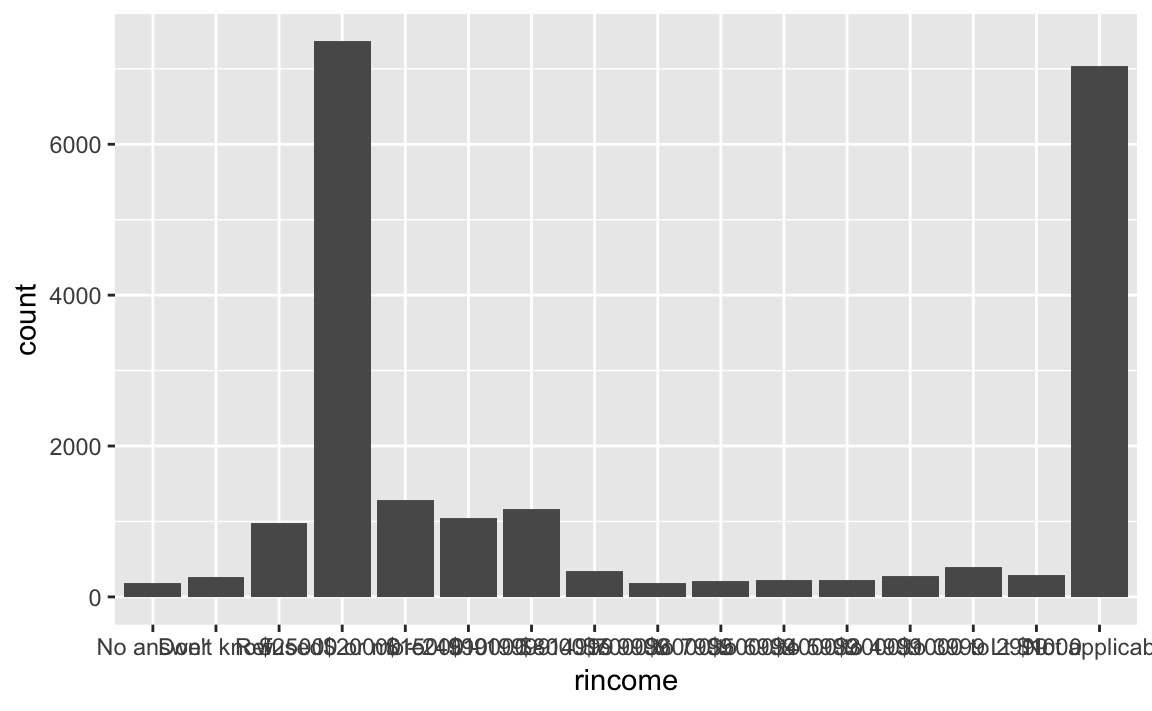
\includegraphics[width=0.7\linewidth]{visualize_files/figure-latex/unnamed-chunk-3-1} \end{center}

An empty plot. The background of the plot is created by
\texttt{ggplot()}, but nothing else is displayed.

\hypertarget{exercise-3.2.4.2.}{%
\subsection*{\texorpdfstring{Exercise
{3.2.4.2}.}{Exercise 3.2.4.2.}}\label{exercise-3.2.4.2.}}
\addcontentsline{toc}{subsection}{Exercise {3.2.4.2}.}

How many rows are in \texttt{mtcars}? How many columns?

There are 32 rows and 11 columns in the \texttt{mtcars} data frame.

\begin{Shaded}
\begin{Highlighting}[]
\KeywordTok{nrow}\NormalTok{(mtcars)}
\CommentTok{#> [1] 32}
\KeywordTok{ncol}\NormalTok{(mtcars)}
\CommentTok{#> [1] 11}
\end{Highlighting}
\end{Shaded}

The number of rows and columns is also displayed by \texttt{glimpse()}:

\begin{Shaded}
\begin{Highlighting}[]
\KeywordTok{glimpse}\NormalTok{(mtcars)}
\CommentTok{#> Observations: 32}
\CommentTok{#> Variables: 11}
\CommentTok{#> $ mpg  <dbl> 21.0, 21.0, 22.8, 21.4, 18.7, 18.1, 14.3, 24.4, 22.8, 19....}
\CommentTok{#> $ cyl  <dbl> 6, 6, 4, 6, 8, 6, 8, 4, 4, 6, 6, 8, 8, 8, 8, 8, 8, 4, 4, ...}
\CommentTok{#> $ disp <dbl> 160.0, 160.0, 108.0, 258.0, 360.0, 225.0, 360.0, 146.7, 1...}
\CommentTok{#> $ hp   <dbl> 110, 110, 93, 110, 175, 105, 245, 62, 95, 123, 123, 180, ...}
\CommentTok{#> $ drat <dbl> 3.90, 3.90, 3.85, 3.08, 3.15, 2.76, 3.21, 3.69, 3.92, 3.9...}
\CommentTok{#> $ wt   <dbl> 2.62, 2.88, 2.32, 3.21, 3.44, 3.46, 3.57, 3.19, 3.15, 3.4...}
\CommentTok{#> $ qsec <dbl> 16.5, 17.0, 18.6, 19.4, 17.0, 20.2, 15.8, 20.0, 22.9, 18....}
\CommentTok{#> $ vs   <dbl> 0, 0, 1, 1, 0, 1, 0, 1, 1, 1, 1, 0, 0, 0, 0, 0, 0, 1, 1, ...}
\CommentTok{#> $ am   <dbl> 1, 1, 1, 0, 0, 0, 0, 0, 0, 0, 0, 0, 0, 0, 0, 0, 0, 1, 1, ...}
\CommentTok{#> $ gear <dbl> 4, 4, 4, 3, 3, 3, 3, 4, 4, 4, 4, 3, 3, 3, 3, 3, 3, 4, 4, ...}
\CommentTok{#> $ carb <dbl> 4, 4, 1, 1, 2, 1, 4, 2, 2, 4, 4, 3, 3, 3, 4, 4, 4, 1, 2, ...}
\end{Highlighting}
\end{Shaded}

\hypertarget{exercise-3.2.4.3.}{%
\subsection*{\texorpdfstring{Exercise
{3.2.4.3}.}{Exercise 3.2.4.3.}}\label{exercise-3.2.4.3.}}
\addcontentsline{toc}{subsection}{Exercise {3.2.4.3}.}

What does the \texttt{drv} variable describe? Read the help for
\texttt{?mpg} to find out.

The \texttt{drv} categorizes cars by which wheels the engine provides
torque to, or drives: the front two wheels, the rear two wheels, or all
four wheels.\footnote{See the Wikipedia article on
  \href{https://en.wikipedia.org/wiki/Automobile_layout}{Automobile
  layout}.}

\begin{longtable}[]{@{}ll@{}}
\toprule
Value & Description\tabularnewline
\midrule
\endhead
\texttt{"f"} &
\href{https://en.wikipedia.org/wiki/Front-wheel_drive}{front-wheel
drive}\tabularnewline
\texttt{"r"} &
\href{https://en.wikipedia.org/wiki/Automobile_layout\#Rear-wheel-drive_layouts}{rear-wheel
drive}\tabularnewline
\texttt{"4"} &
\href{https://en.wikipedia.org/wiki/Four-wheel_drive}{four-wheel
drive}\tabularnewline
\bottomrule
\end{longtable}

\hypertarget{exercise-3.2.4.4.}{%
\subsection*{\texorpdfstring{Exercise
{3.2.4.4}.}{Exercise 3.2.4.4.}}\label{exercise-3.2.4.4.}}
\addcontentsline{toc}{subsection}{Exercise {3.2.4.4}.}

Make a scatter plot of \texttt{hwy} vs \texttt{cyl}.

\begin{Shaded}
\begin{Highlighting}[]
\KeywordTok{ggplot}\NormalTok{(mpg, }\KeywordTok{aes}\NormalTok{(}\DataTypeTok{x =}\NormalTok{ hwy, }\DataTypeTok{y =}\NormalTok{ cyl)) }\OperatorTok{+}
\StringTok{  }\KeywordTok{geom_point}\NormalTok{()}
\end{Highlighting}
\end{Shaded}

\begin{center}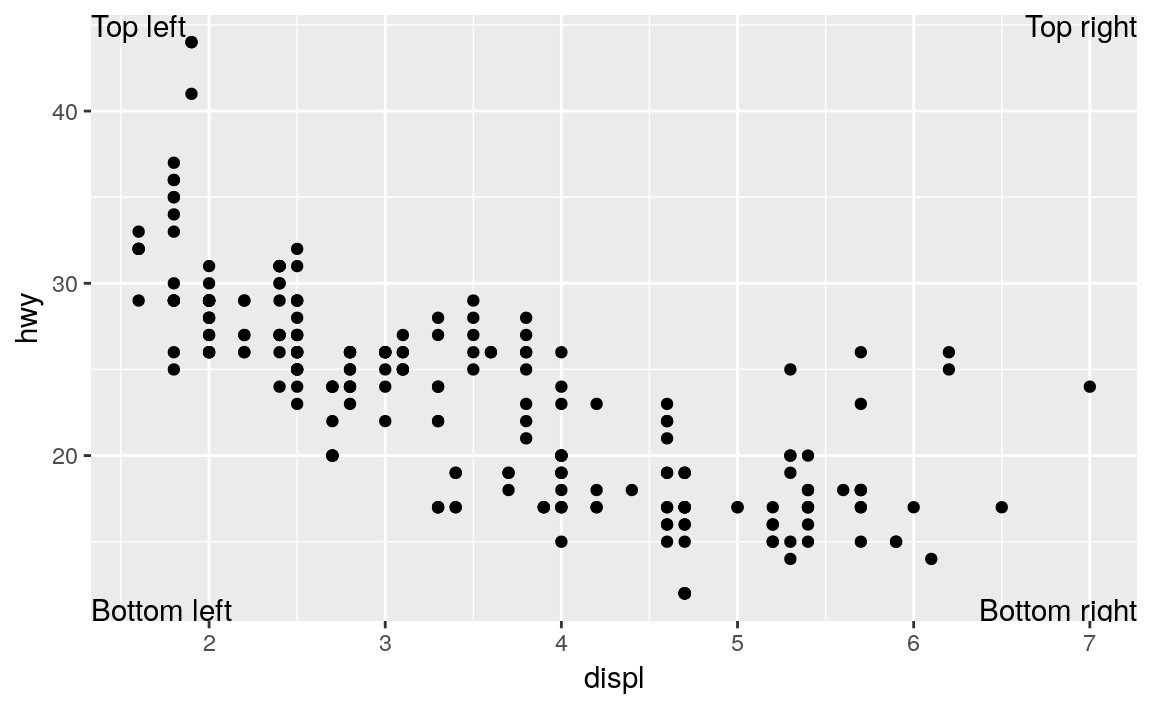
\includegraphics[width=0.7\linewidth]{visualize_files/figure-latex/unnamed-chunk-6-1} \end{center}

\hypertarget{exercise-3.2.4.5.}{%
\subsection*{\texorpdfstring{Exercise
{3.2.4.5}.}{Exercise 3.2.4.5.}}\label{exercise-3.2.4.5.}}
\addcontentsline{toc}{subsection}{Exercise {3.2.4.5}.}

What happens if you make a scatter plot of \texttt{class} vs
\texttt{drv}. Why is the plot not useful?

\begin{Shaded}
\begin{Highlighting}[]
\KeywordTok{ggplot}\NormalTok{(mpg, }\KeywordTok{aes}\NormalTok{(}\DataTypeTok{x =}\NormalTok{ class, }\DataTypeTok{y =}\NormalTok{ drv)) }\OperatorTok{+}
\StringTok{  }\KeywordTok{geom_point}\NormalTok{()}
\end{Highlighting}
\end{Shaded}

\begin{center}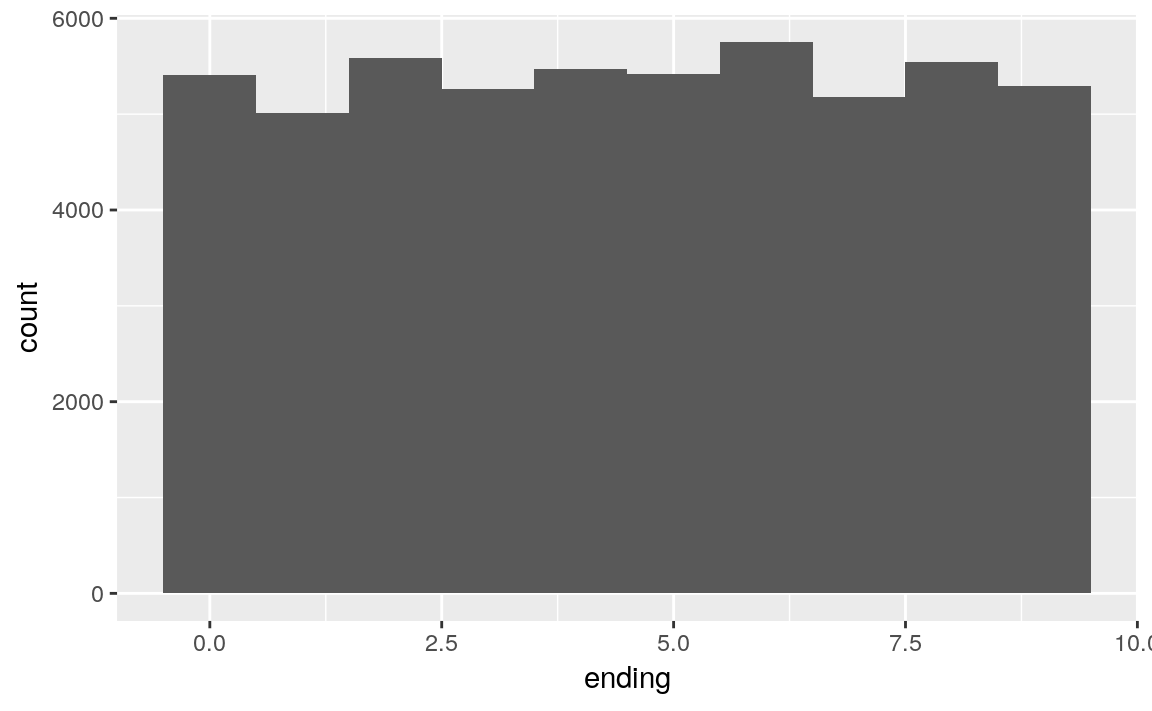
\includegraphics[width=0.7\linewidth]{visualize_files/figure-latex/unnamed-chunk-7-1} \end{center}

A scatter plot is not a useful way to plot these variables, since both
\texttt{drv} and \texttt{class} are factor variables taking a limited
number of values.

\begin{Shaded}
\begin{Highlighting}[]
\KeywordTok{count}\NormalTok{(mpg, drv, class)}
\CommentTok{#> # A tibble: 12 x 3}
\CommentTok{#>   drv   class          n}
\CommentTok{#>   <chr> <chr>      <int>}
\CommentTok{#> 1 4     compact       12}
\CommentTok{#> 2 4     midsize        3}
\CommentTok{#> 3 4     pickup        33}
\CommentTok{#> 4 4     subcompact     4}
\CommentTok{#> 5 4     suv           51}
\CommentTok{#> 6 f     compact       35}
\CommentTok{#> # ... with 6 more rows}
\end{Highlighting}
\end{Shaded}

The scatter plot cannot show which are overlapping or not. Later
chapters discuss means to deal with this, including alternative plots
and jittering the points so they don't overlap.

\hypertarget{aesthetic-mappings}{%
\section{Aesthetic mappings}\label{aesthetic-mappings}}

\hypertarget{exercise-3.3.1.1}{%
\subsection*{\texorpdfstring{Exercise
{3.3.1.1}}{Exercise 3.3.1.1}}\label{exercise-3.3.1.1}}
\addcontentsline{toc}{subsection}{Exercise {3.3.1.1}}

What's gone wrong with this code? Why are the points not blue?

\begin{Shaded}
\begin{Highlighting}[]
\KeywordTok{ggplot}\NormalTok{(}\DataTypeTok{data =}\NormalTok{ mpg) }\OperatorTok{+}
\StringTok{  }\KeywordTok{geom_point}\NormalTok{(}\DataTypeTok{mapping =} \KeywordTok{aes}\NormalTok{(}\DataTypeTok{x =}\NormalTok{ displ, }\DataTypeTok{y =}\NormalTok{ hwy, }\DataTypeTok{colour =} \StringTok{"blue"}\NormalTok{))}
\end{Highlighting}
\end{Shaded}

\begin{center}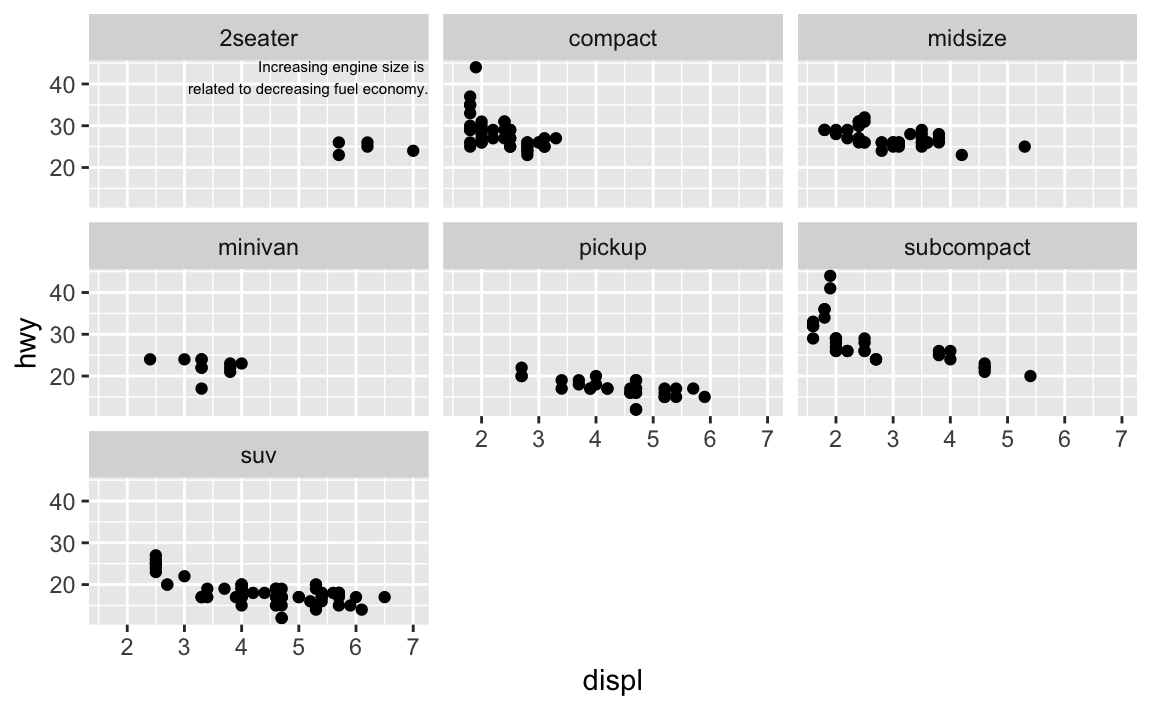
\includegraphics[width=0.7\linewidth]{visualize_files/figure-latex/unnamed-chunk-9-1} \end{center}

Since \texttt{colour\ =\ "blue"} was included within the
\texttt{mapping} argument, it was treated as an aesthetic (a mapping
between a variable and a value). The expression, \texttt{color="blue"},
treats \texttt{"blue"} as a variable with only one value:
\texttt{"blue"}. If this is confusing, consider how
\texttt{colour\ =\ 1:234} or \texttt{colour\ =\ 1} would be interpreted
by \texttt{aes()}.

\hypertarget{exercise-3.3.1.2}{%
\subsection*{\texorpdfstring{Exercise
{3.3.1.2}}{Exercise 3.3.1.2}}\label{exercise-3.3.1.2}}
\addcontentsline{toc}{subsection}{Exercise {3.3.1.2}}

Which variables in \texttt{mpg} are categorical? Which variables are
continuous? (Hint: type \texttt{?mpg} to read the documentation for the
dataset). How can you see this information when you run \texttt{mpg}?

\begin{Shaded}
\begin{Highlighting}[]
\NormalTok{?mpg}
\end{Highlighting}
\end{Shaded}

When printing the data frame, this information is given at the top of
each column within angled brackets. Categorical variables have a class
of ``character'' (\texttt{\textless{}chr\textgreater{}}).

\begin{Shaded}
\begin{Highlighting}[]
\NormalTok{mpg}
\CommentTok{#> # A tibble: 234 x 11}
\CommentTok{#>   manufacturer model displ  year   cyl trans drv     cty   hwy fl    class}
\CommentTok{#>   <chr>        <chr> <dbl> <int> <int> <chr> <chr> <int> <int> <chr> <chr>}
\CommentTok{#> 1 audi         a4      1.8  1999     4 auto~ f        18    29 p     comp~}
\CommentTok{#> 2 audi         a4      1.8  1999     4 manu~ f        21    29 p     comp~}
\CommentTok{#> 3 audi         a4      2    2008     4 manu~ f        20    31 p     comp~}
\CommentTok{#> 4 audi         a4      2    2008     4 auto~ f        21    30 p     comp~}
\CommentTok{#> 5 audi         a4      2.8  1999     6 auto~ f        16    26 p     comp~}
\CommentTok{#> 6 audi         a4      2.8  1999     6 manu~ f        18    26 p     comp~}
\CommentTok{#> # ... with 228 more rows}
\end{Highlighting}
\end{Shaded}

Alternatively, \texttt{glimpse()} displays the type of each column:

\begin{Shaded}
\begin{Highlighting}[]
\KeywordTok{glimpse}\NormalTok{(mpg)}
\CommentTok{#> Observations: 234}
\CommentTok{#> Variables: 11}
\CommentTok{#> $ manufacturer <chr> "audi", "audi", "audi", "audi", "audi", "audi", "...}
\CommentTok{#> $ model        <chr> "a4", "a4", "a4", "a4", "a4", "a4", "a4", "a4 qua...}
\CommentTok{#> $ displ        <dbl> 1.8, 1.8, 2.0, 2.0, 2.8, 2.8, 3.1, 1.8, 1.8, 2.0,...}
\CommentTok{#> $ year         <int> 1999, 1999, 2008, 2008, 1999, 1999, 2008, 1999, 1...}
\CommentTok{#> $ cyl          <int> 4, 4, 4, 4, 6, 6, 6, 4, 4, 4, 4, 6, 6, 6, 6, 6, 6...}
\CommentTok{#> $ trans        <chr> "auto(l5)", "manual(m5)", "manual(m6)", "auto(av)...}
\CommentTok{#> $ drv          <chr> "f", "f", "f", "f", "f", "f", "f", "4", "4", "4",...}
\CommentTok{#> $ cty          <int> 18, 21, 20, 21, 16, 18, 18, 18, 16, 20, 19, 15, 1...}
\CommentTok{#> $ hwy          <int> 29, 29, 31, 30, 26, 26, 27, 26, 25, 28, 27, 25, 2...}
\CommentTok{#> $ fl           <chr> "p", "p", "p", "p", "p", "p", "p", "p", "p", "p",...}
\CommentTok{#> $ class        <chr> "compact", "compact", "compact", "compact", "comp...}
\end{Highlighting}
\end{Shaded}

\hypertarget{exercise-3.3.1.3}{%
\subsection*{\texorpdfstring{Exercise
{3.3.1.3}}{Exercise 3.3.1.3}}\label{exercise-3.3.1.3}}
\addcontentsline{toc}{subsection}{Exercise {3.3.1.3}}

Map a continuous variable to color, size, and shape. How do these
aesthetics behave differently for categorical vs.~continuous variables?

The variable \texttt{cty}, city highway miles per gallon, is a
continuous variable:

\begin{Shaded}
\begin{Highlighting}[]
\KeywordTok{ggplot}\NormalTok{(mpg, }\KeywordTok{aes}\NormalTok{(}\DataTypeTok{x =}\NormalTok{ displ, }\DataTypeTok{y =}\NormalTok{ hwy, }\DataTypeTok{colour =}\NormalTok{ cty)) }\OperatorTok{+}
\StringTok{  }\KeywordTok{geom_point}\NormalTok{()}
\end{Highlighting}
\end{Shaded}

\begin{center}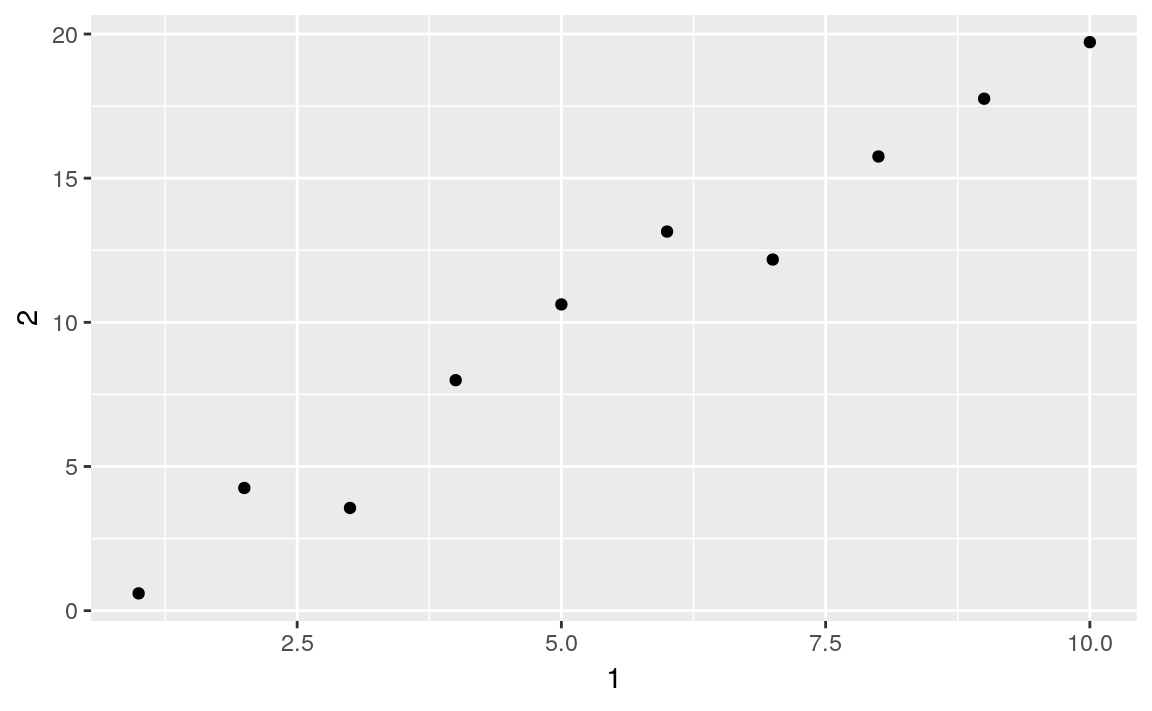
\includegraphics[width=0.7\linewidth]{visualize_files/figure-latex/unnamed-chunk-13-1} \end{center}

Instead of using discrete colors, the continuous variable uses a scale
that varies from a light to dark blue color.

\begin{Shaded}
\begin{Highlighting}[]
\KeywordTok{ggplot}\NormalTok{(mpg, }\KeywordTok{aes}\NormalTok{(}\DataTypeTok{x =}\NormalTok{ displ, }\DataTypeTok{y =}\NormalTok{ hwy, }\DataTypeTok{size =}\NormalTok{ cty)) }\OperatorTok{+}
\StringTok{  }\KeywordTok{geom_point}\NormalTok{()}
\end{Highlighting}
\end{Shaded}

\begin{center}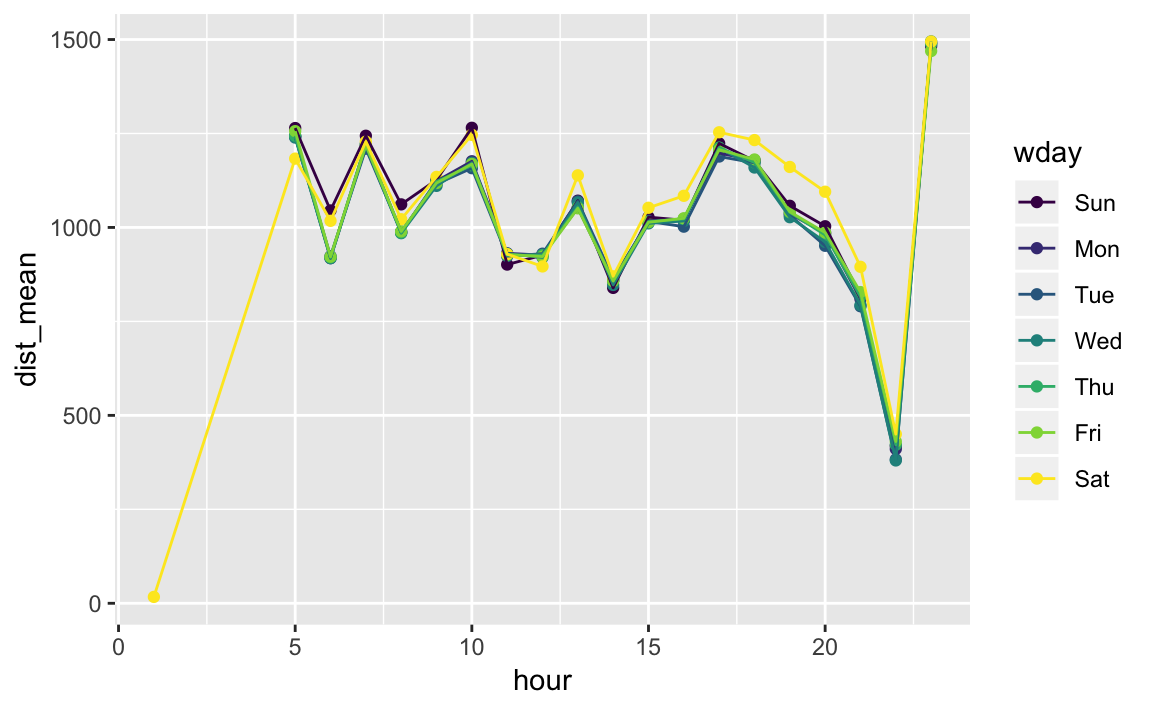
\includegraphics[width=0.7\linewidth]{visualize_files/figure-latex/unnamed-chunk-14-1} \end{center}

When mapped to size, the sizes of the points vary continuously with
respect to the size (although the legend shows a few representative
values)

\begin{Shaded}
\begin{Highlighting}[]
\KeywordTok{ggplot}\NormalTok{(mpg, }\KeywordTok{aes}\NormalTok{(}\DataTypeTok{x =}\NormalTok{ displ, }\DataTypeTok{y =}\NormalTok{ hwy, }\DataTypeTok{shape =}\NormalTok{ cty)) }\OperatorTok{+}
\StringTok{  }\KeywordTok{geom_point}\NormalTok{()}
\CommentTok{#> Error: A continuous variable can not be mapped to shape}
\end{Highlighting}
\end{Shaded}

\begin{center}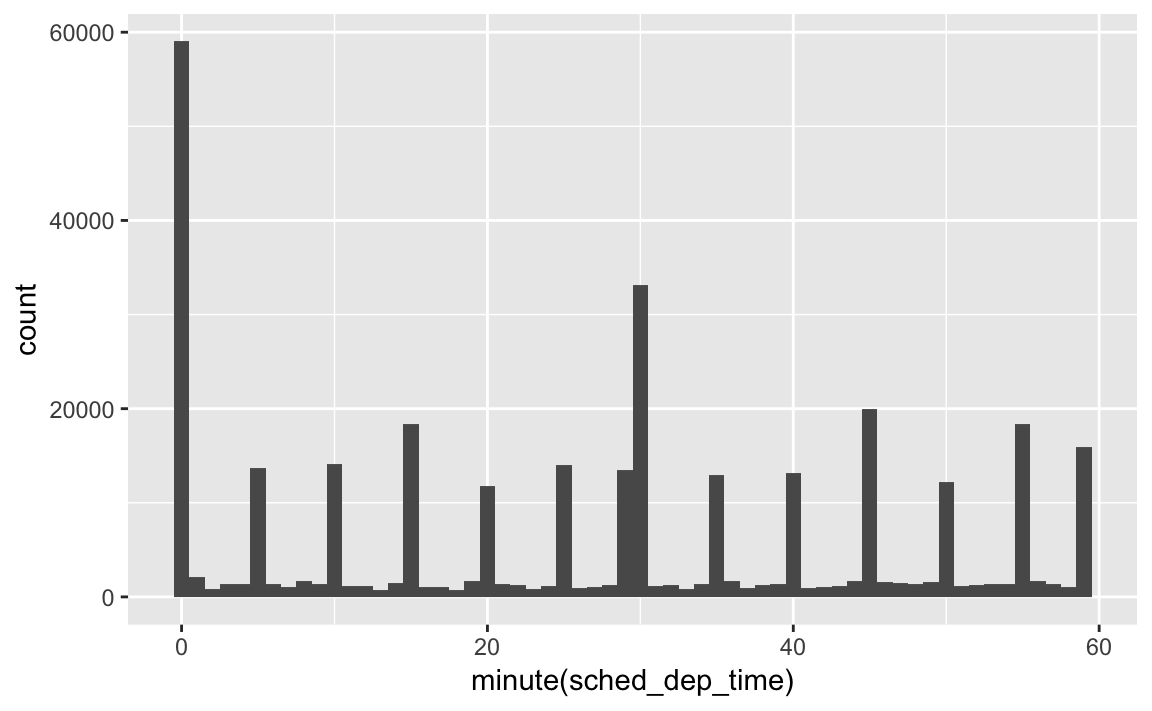
\includegraphics[width=0.7\linewidth]{visualize_files/figure-latex/unnamed-chunk-15-1} \end{center}

When a continuous value is mapped to shape, it gives an error. Though we
could split a continuous variable into discrete categories and use a
shape aesthetic, this would conceptually not make sense. A continuous
numeric variable is ordered, but shapes have no natural order. It is
clear that smaller points correspond to smaller values, or once the
color scale is given, which colors correspond to larger or smaller
values. But it is not clear whether a square is greater or less than a
circle.

\hypertarget{exercise-3.3.1.4}{%
\subsection*{\texorpdfstring{Exercise
{3.3.1.4}}{Exercise 3.3.1.4}}\label{exercise-3.3.1.4}}
\addcontentsline{toc}{subsection}{Exercise {3.3.1.4}}

What happens if you map the same variable to multiple aesthetics?

\begin{Shaded}
\begin{Highlighting}[]
\KeywordTok{ggplot}\NormalTok{(mpg, }\KeywordTok{aes}\NormalTok{(}\DataTypeTok{x =}\NormalTok{ displ, }\DataTypeTok{y =}\NormalTok{ hwy, }\DataTypeTok{colour =}\NormalTok{ hwy, }\DataTypeTok{size =}\NormalTok{ displ)) }\OperatorTok{+}
\StringTok{  }\KeywordTok{geom_point}\NormalTok{()}
\end{Highlighting}
\end{Shaded}

\begin{center}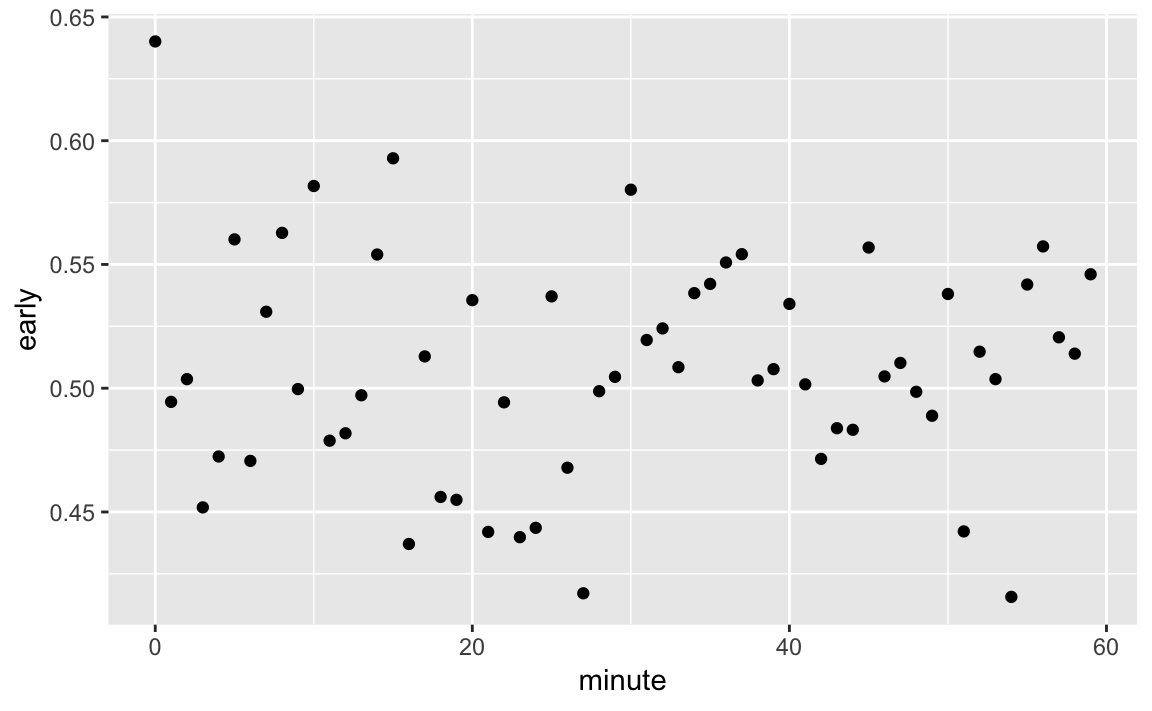
\includegraphics[width=0.7\linewidth]{visualize_files/figure-latex/unnamed-chunk-16-1} \end{center}

In the above plot, \texttt{hwy} is mapped to both location on the y-axis
and color, and \texttt{displ} is mapped to both location on the x-axis
and size. The code works and produces a plot, even if it is a bad one.
Mapping a single variable to multiple aesthetics is redundant. Because
it is redundant information, in most cases avoid mapping a single
variable to multiple aesthetics.

\hypertarget{exercise-3.3.1.5}{%
\subsection*{\texorpdfstring{Exercise
{3.3.1.5}}{Exercise 3.3.1.5}}\label{exercise-3.3.1.5}}
\addcontentsline{toc}{subsection}{Exercise {3.3.1.5}}

What does the stroke aesthetic do? What shapes does it work with? (Hint:
use \texttt{?geom\_point})

Stroke changes the size of the border for shapes (21-25). These are
filled shapes in which the color and size of the border can differ from
that of the filled interior of the shape.

For example

\begin{Shaded}
\begin{Highlighting}[]
\KeywordTok{ggplot}\NormalTok{(mtcars, }\KeywordTok{aes}\NormalTok{(wt, mpg)) }\OperatorTok{+}
\StringTok{  }\KeywordTok{geom_point}\NormalTok{(}\DataTypeTok{shape =} \DecValTok{21}\NormalTok{, }\DataTypeTok{colour =} \StringTok{"black"}\NormalTok{, }\DataTypeTok{fill =} \StringTok{"white"}\NormalTok{, }\DataTypeTok{size =} \DecValTok{5}\NormalTok{, }\DataTypeTok{stroke =} \DecValTok{5}\NormalTok{)}
\end{Highlighting}
\end{Shaded}

\begin{center}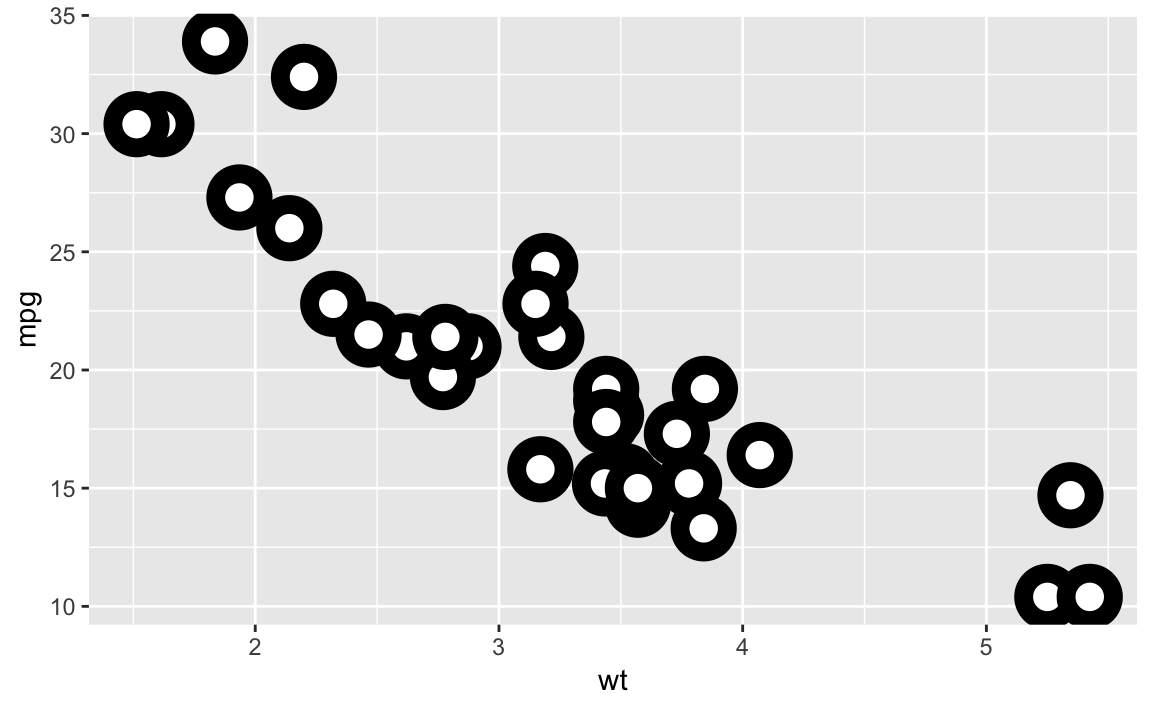
\includegraphics[width=0.7\linewidth]{visualize_files/figure-latex/ex.3.3.1.5-1} \end{center}

\hypertarget{exercise-3.3.1.6.}{%
\subsection*{\texorpdfstring{Exercise
{3.3.1.6}.}{Exercise 3.3.1.6.}}\label{exercise-3.3.1.6.}}
\addcontentsline{toc}{subsection}{Exercise {3.3.1.6}.}

What happens if you map an aesthetic to something other than a variable
name, like \texttt{aes(colour\ =\ displ\ \textless{}\ 5)}?

\begin{Shaded}
\begin{Highlighting}[]
\KeywordTok{ggplot}\NormalTok{(mpg, }\KeywordTok{aes}\NormalTok{(}\DataTypeTok{x =}\NormalTok{ displ, }\DataTypeTok{y =}\NormalTok{ hwy, }\DataTypeTok{colour =}\NormalTok{ displ }\OperatorTok{<}\StringTok{ }\DecValTok{5}\NormalTok{)) }\OperatorTok{+}
\StringTok{  }\KeywordTok{geom_point}\NormalTok{()}
\end{Highlighting}
\end{Shaded}

\begin{center}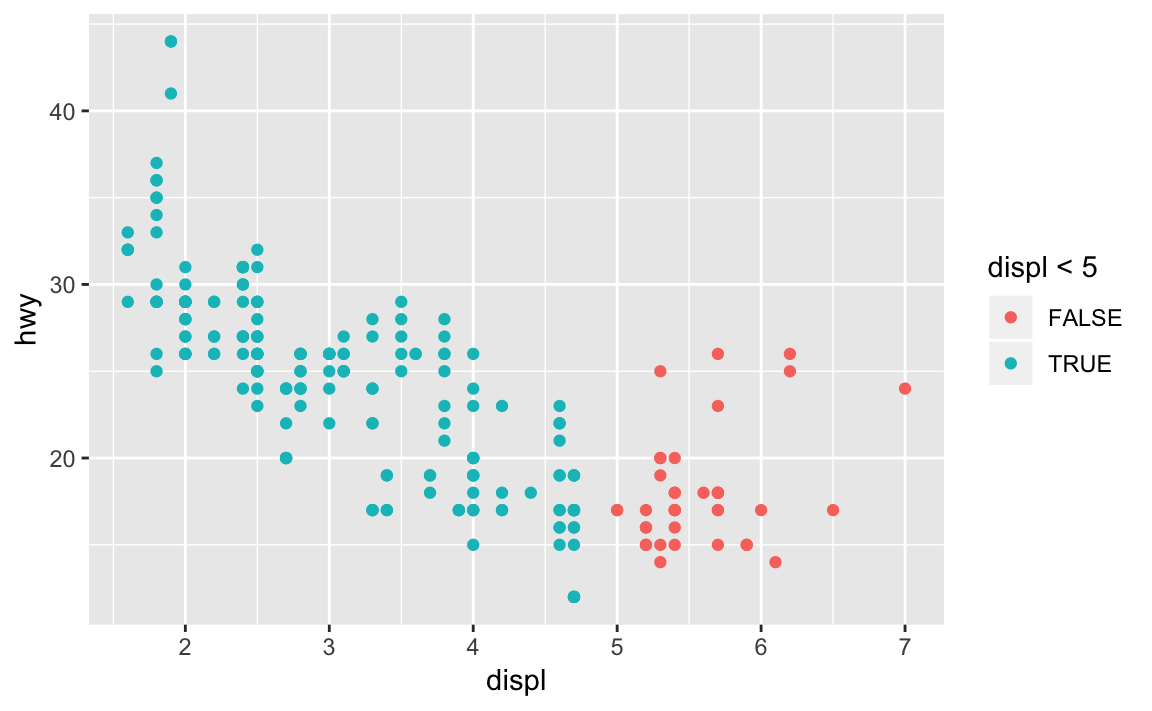
\includegraphics[width=0.7\linewidth]{visualize_files/figure-latex/ex.3.3.1.6-1} \end{center}

Aesthetics can also be mapped to expressions (code like
\texttt{displ\ \textless{}\ 5}). It will create a temporary variable
which takes values from the result of the expression. In this case, it
is logical variable which is \texttt{TRUE} or \texttt{FALSE}. This also
explains exercise 1, \texttt{colour\ =\ "blue"} created a categorical
variable that only had one category: ``blue''.

\hypertarget{common-problems}{%
\section{Common problems}\label{common-problems}}

No exercises

\hypertarget{facets}{%
\section{Facets}\label{facets}}

\hypertarget{exercise-3.5.1.1}{%
\subsection*{\texorpdfstring{Exercise
{3.5.1.1}}{Exercise 3.5.1.1}}\label{exercise-3.5.1.1}}
\addcontentsline{toc}{subsection}{Exercise {3.5.1.1}}

What happens if you facet on a continuous variable?

Let's see.

\begin{Shaded}
\begin{Highlighting}[]
\KeywordTok{ggplot}\NormalTok{(mpg, }\KeywordTok{aes}\NormalTok{(}\DataTypeTok{x =}\NormalTok{ displ, }\DataTypeTok{y =}\NormalTok{ hwy)) }\OperatorTok{+}
\StringTok{  }\KeywordTok{geom_point}\NormalTok{() }\OperatorTok{+}
\StringTok{  }\KeywordTok{facet_grid}\NormalTok{(. }\OperatorTok{~}\StringTok{ }\NormalTok{cty)}
\end{Highlighting}
\end{Shaded}

\begin{center}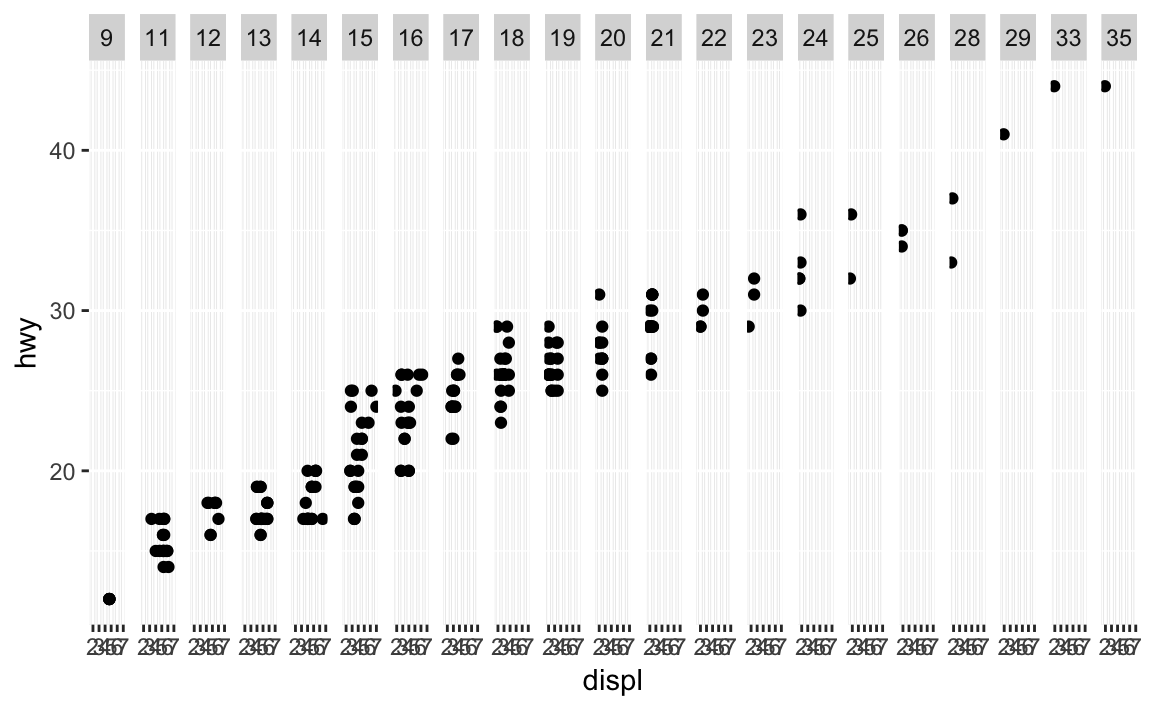
\includegraphics[width=0.7\linewidth]{visualize_files/figure-latex/ex.3.5.1.1-1} \end{center}

It converts the continuous variable to a factor and creates facets for
\textbf{all} unique values of it.

\hypertarget{exercise-3.5.1.2}{%
\subsection*{\texorpdfstring{Exercise
{3.5.1.2}}{Exercise 3.5.1.2}}\label{exercise-3.5.1.2}}
\addcontentsline{toc}{subsection}{Exercise {3.5.1.2}}

What do the empty cells in plot with
\texttt{facet\_grid(drv\ \textasciitilde{}\ cyl)} mean? How do they
relate to this plot?

They are cells in which there are no values of the combination of
\texttt{drv} and \texttt{cyl}.

\begin{Shaded}
\begin{Highlighting}[]
\KeywordTok{ggplot}\NormalTok{(}\DataTypeTok{data =}\NormalTok{ mpg) }\OperatorTok{+}
\StringTok{  }\KeywordTok{geom_point}\NormalTok{(}\DataTypeTok{mapping =} \KeywordTok{aes}\NormalTok{(}\DataTypeTok{x =}\NormalTok{ drv, }\DataTypeTok{y =}\NormalTok{ cyl))}
\end{Highlighting}
\end{Shaded}

\begin{center}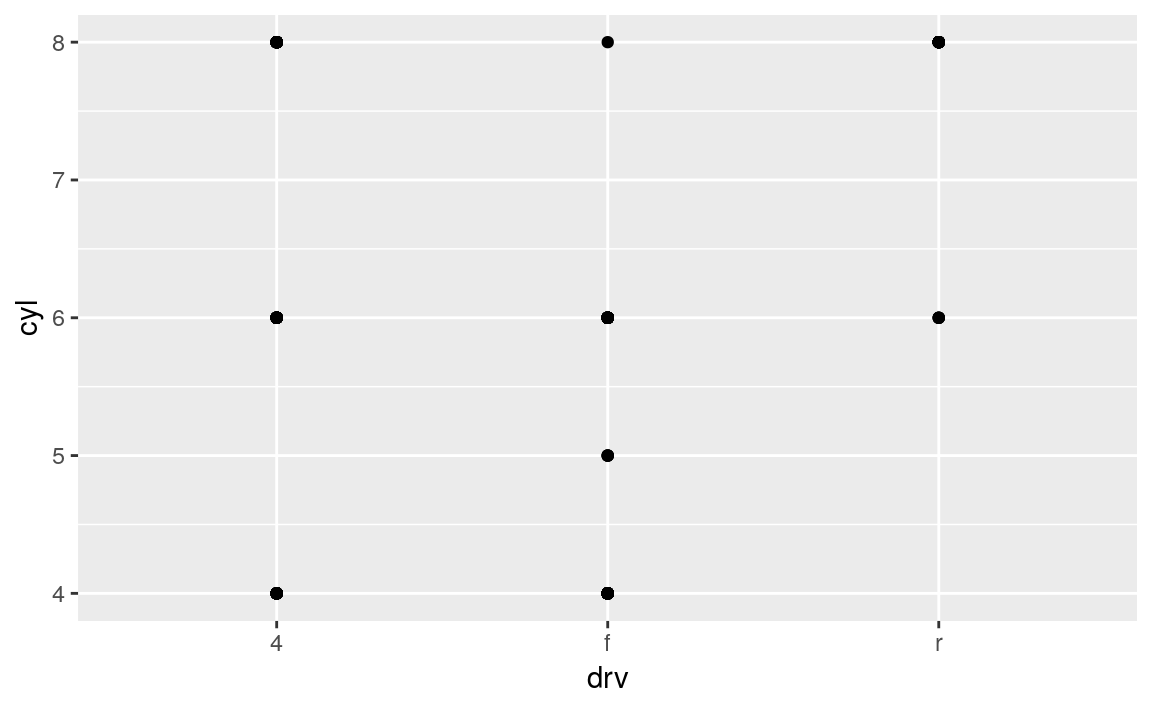
\includegraphics[width=0.7\linewidth]{visualize_files/figure-latex/unnamed-chunk-17-1} \end{center}

The locations in the above plot without points are the same cells in
\texttt{facet\_grid(drv\ \textasciitilde{}\ cyl)} that have no points.

\hypertarget{exercise-3.5.1.3}{%
\subsection*{\texorpdfstring{Exercise
{3.5.1.3}}{Exercise 3.5.1.3}}\label{exercise-3.5.1.3}}
\addcontentsline{toc}{subsection}{Exercise {3.5.1.3}}

What plots does the following code make? What does \texttt{.} do?

The symbol \texttt{.} ignores that dimension for faceting.

This plot facets by values of \texttt{drv} on the y-axis:

\begin{Shaded}
\begin{Highlighting}[]
\KeywordTok{ggplot}\NormalTok{(}\DataTypeTok{data =}\NormalTok{ mpg) }\OperatorTok{+}
\StringTok{  }\KeywordTok{geom_point}\NormalTok{(}\DataTypeTok{mapping =} \KeywordTok{aes}\NormalTok{(}\DataTypeTok{x =}\NormalTok{ displ, }\DataTypeTok{y =}\NormalTok{ hwy)) }\OperatorTok{+}
\StringTok{  }\KeywordTok{facet_grid}\NormalTok{(drv }\OperatorTok{~}\StringTok{ }\NormalTok{.)}
\end{Highlighting}
\end{Shaded}

\begin{center}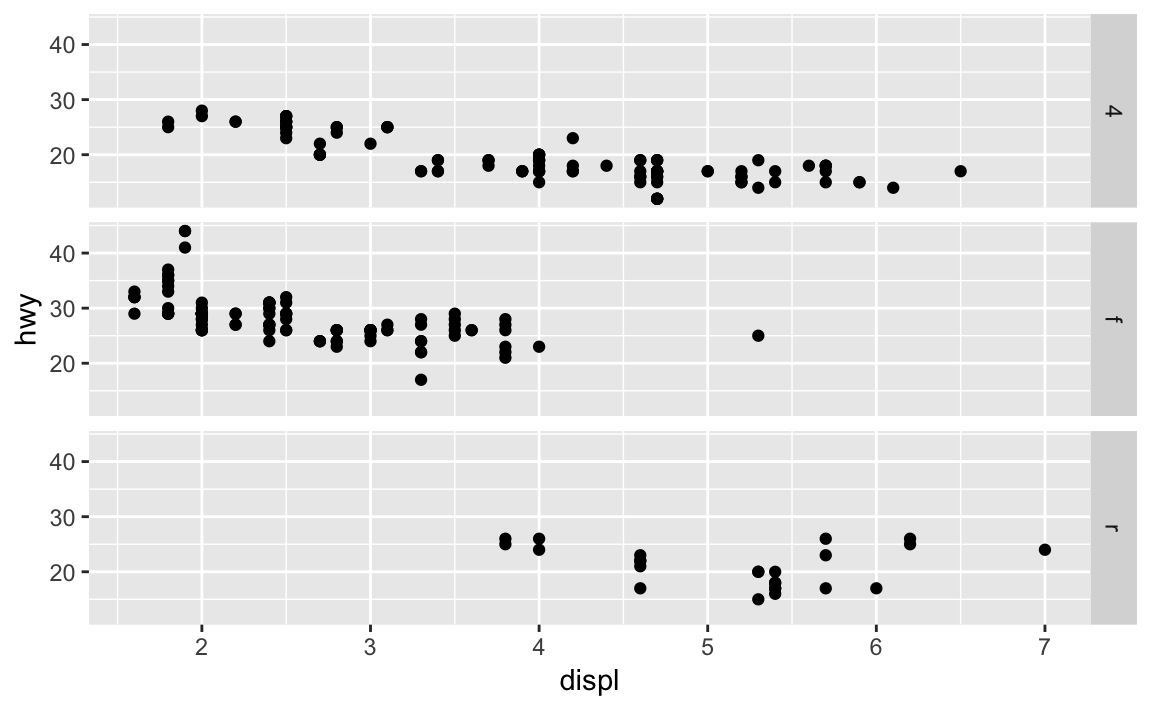
\includegraphics[width=0.7\linewidth]{visualize_files/figure-latex/ex.3.5.1.4.a-1} \end{center}

This plot facets by values of \texttt{cyl} on the x-axis:

\begin{Shaded}
\begin{Highlighting}[]
\KeywordTok{ggplot}\NormalTok{(}\DataTypeTok{data =}\NormalTok{ mpg) }\OperatorTok{+}
\StringTok{  }\KeywordTok{geom_point}\NormalTok{(}\DataTypeTok{mapping =} \KeywordTok{aes}\NormalTok{(}\DataTypeTok{x =}\NormalTok{ displ, }\DataTypeTok{y =}\NormalTok{ hwy)) }\OperatorTok{+}
\StringTok{  }\KeywordTok{facet_grid}\NormalTok{(. }\OperatorTok{~}\StringTok{ }\NormalTok{cyl)}
\end{Highlighting}
\end{Shaded}

\begin{center}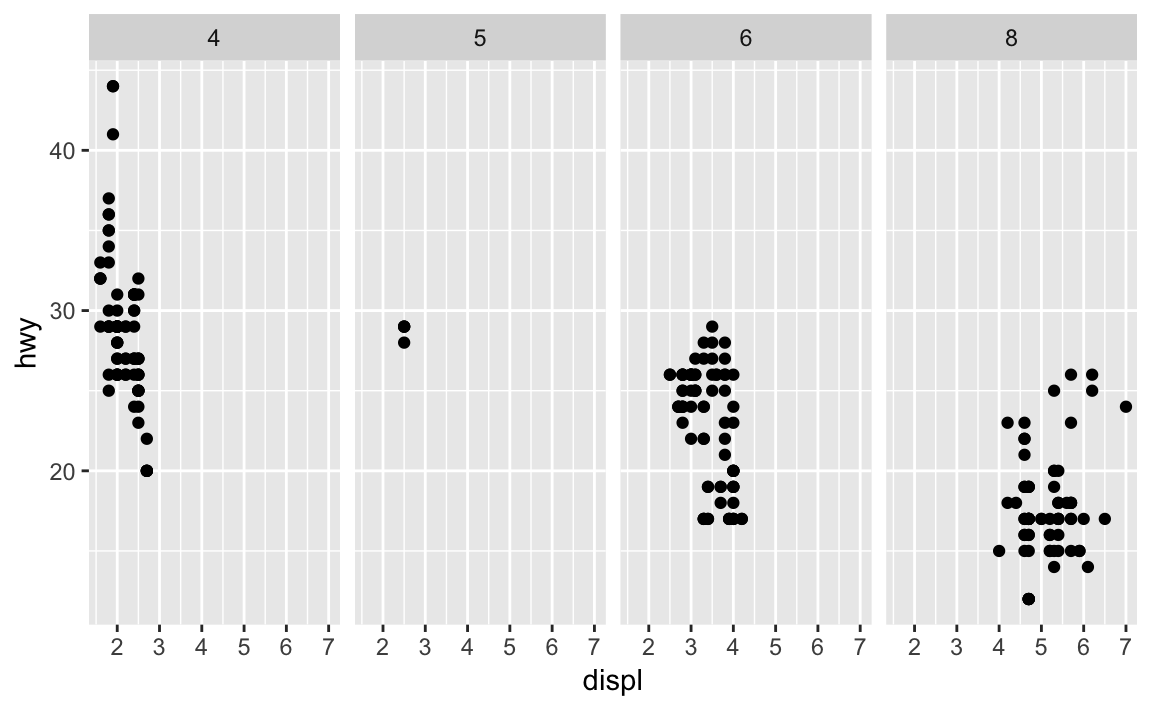
\includegraphics[width=0.7\linewidth]{visualize_files/figure-latex/ex.3.5.1.4.b-1} \end{center}

\hypertarget{exercise-3.5.1.4}{%
\subsection*{\texorpdfstring{Exercise
{3.5.1.4}}{Exercise 3.5.1.4}}\label{exercise-3.5.1.4}}
\addcontentsline{toc}{subsection}{Exercise {3.5.1.4}}

Take the first faceted plot in this section:

\begin{Shaded}
\begin{Highlighting}[]
\KeywordTok{ggplot}\NormalTok{(}\DataTypeTok{data =}\NormalTok{ mpg) }\OperatorTok{+}
\StringTok{  }\KeywordTok{geom_point}\NormalTok{(}\DataTypeTok{mapping =} \KeywordTok{aes}\NormalTok{(}\DataTypeTok{x =}\NormalTok{ displ, }\DataTypeTok{y =}\NormalTok{ hwy)) }\OperatorTok{+}
\StringTok{  }\KeywordTok{facet_wrap}\NormalTok{(}\OperatorTok{~}\StringTok{ }\NormalTok{class, }\DataTypeTok{nrow =} \DecValTok{2}\NormalTok{)}
\end{Highlighting}
\end{Shaded}

\begin{center}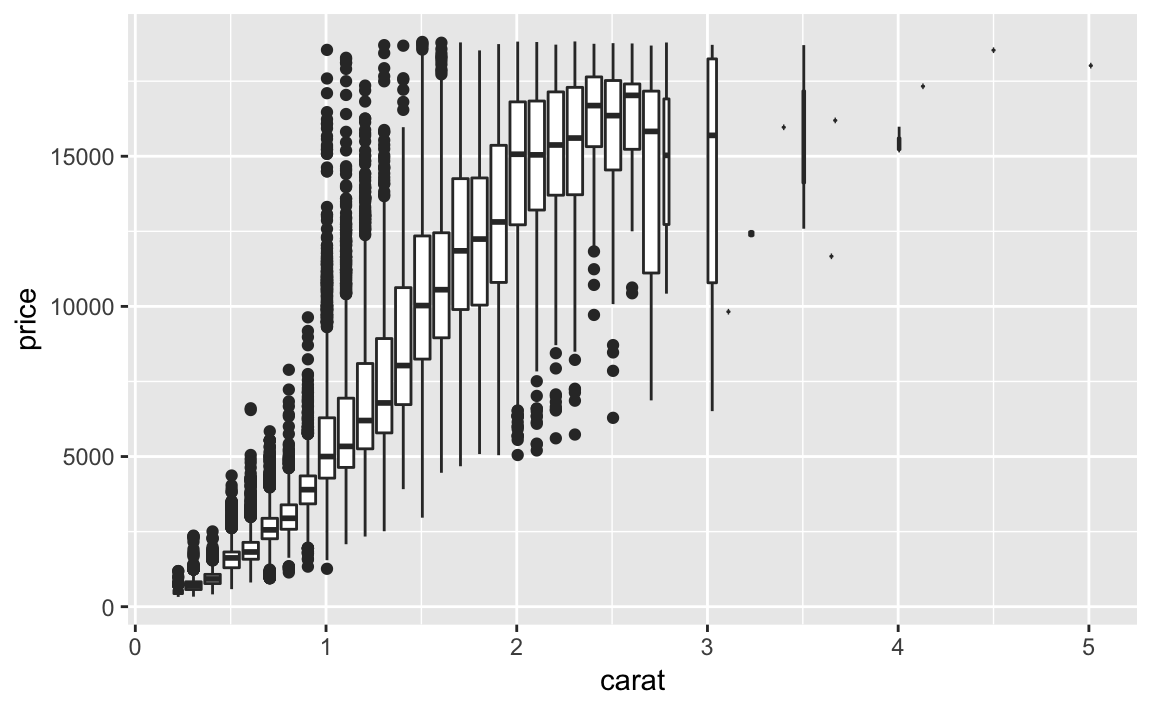
\includegraphics[width=0.7\linewidth]{visualize_files/figure-latex/unnamed-chunk-18-1} \end{center}

What are the advantages to using faceting instead of the colour
aesthetic? What are the disadvantages? How might the balance change if
you had a larger dataset?

This is what the plot looks like when \texttt{class} is represented by
the colour the color aesthetic instead of faceting.

\begin{Shaded}
\begin{Highlighting}[]
\KeywordTok{ggplot}\NormalTok{(}\DataTypeTok{data =}\NormalTok{ mpg) }\OperatorTok{+}
\StringTok{  }\KeywordTok{geom_point}\NormalTok{(}\DataTypeTok{mapping =} \KeywordTok{aes}\NormalTok{(}\DataTypeTok{x =}\NormalTok{ displ, }\DataTypeTok{y =}\NormalTok{ hwy, }\DataTypeTok{color =}\NormalTok{ class))}
\end{Highlighting}
\end{Shaded}

\begin{center}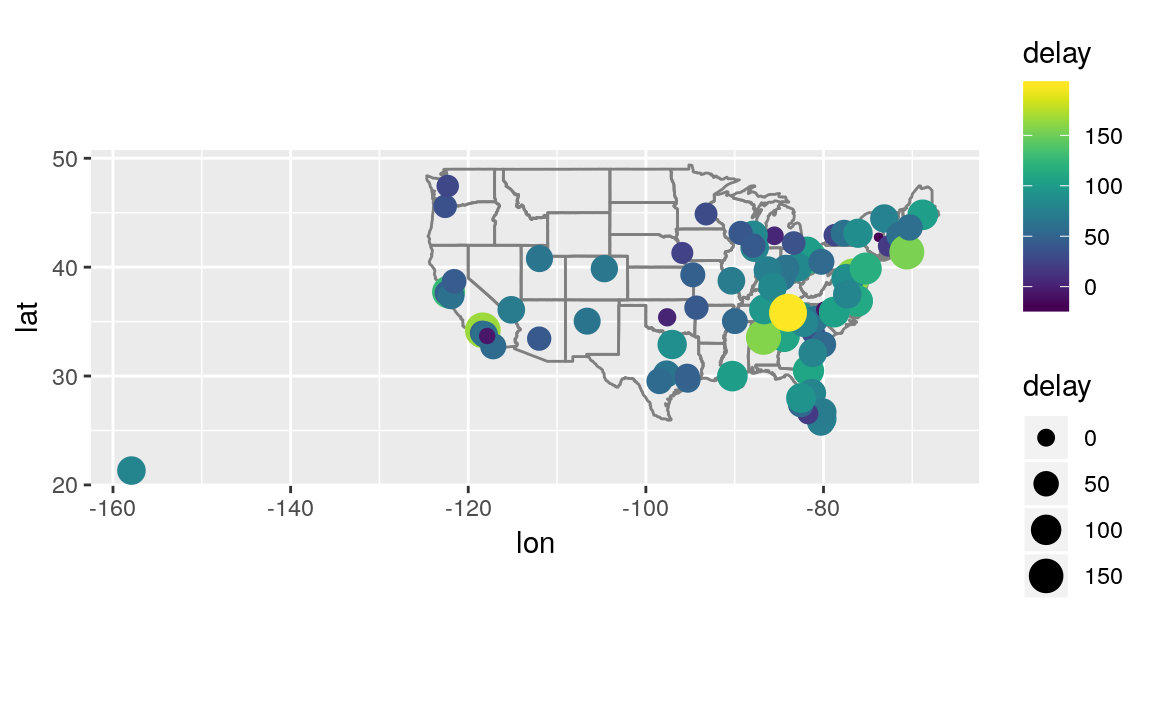
\includegraphics[width=0.7\linewidth]{visualize_files/figure-latex/unnamed-chunk-19-1} \end{center}

Advantages of encoding \texttt{class} with facets instead of color
include the ability to encode more distinct categories. For me, it is
difficult to distinguish color of \texttt{"midsize"} and the teal of
\texttt{"minivan"} points are difficult to distinguish. Given human
visual perception, the max number of colors to use when encoding
unordered categorical (qualitative) data is nine, and in practice, often
much less than that. Also, while placing points in different categories
in different scales makes it difficult to directly compare values of
individual points in different categories, it can make it easier to
compare patterns between categories.

Disadvantages of encoding \texttt{class} with facets instead of color
are that different the different class is that the points for each
category are on different plots, making it more difficult to directly
compare the locations of individual points. Using the same x- and
y-scales for all facets lessens this disadvantage. Since encoding class
within color also places all points on the same plot, it visualizes the
unconditional relationship between the x and y variables; with facets,
the unconditional relationship is no longer visualized since the points
are spread across multiple plots.

The benefits encoding a variable through facetting over color become
more advantageous as either the number of points or the number of
categories increase. In the former, as the number of points increase,
there is likely to be more overlap.

It is difficult to handle overlapping points with color. Jittering will
still work with color. But jittering will only work well if there are
few points and the classes do not overlap much, otherwise the colors of
areas will no longer be distinct and it will be hard to visually pick
out the patterns of different categories. Transparency (\texttt{alpha})
does not work well with colors since the mixing of overlapping
transparent colors will no longer represent the colors of the
categories. Binning methods use already color to encode density, so
color cannot be used to encode categories.

As noted before, as the number of categories increases, the difference
between colors decreases, to the point that the color of categories will
no longer be visually distinct.

\hypertarget{exercise-3.5.1.5}{%
\subsection*{\texorpdfstring{Exercise
{3.5.1.5}}{Exercise 3.5.1.5}}\label{exercise-3.5.1.5}}
\addcontentsline{toc}{subsection}{Exercise {3.5.1.5}}

Read \texttt{?facet\_wrap}. What does \texttt{nrow} do? What does
\texttt{ncol} do? What other options control the layout of the
individual panels? Why doesn't \texttt{facet\_grid()} have \texttt{nrow}
and \texttt{ncol} variables?

The arguments \texttt{nrow} (\texttt{ncol}) determines the number of
rows (columns) to use when laying out the facets. It is necessary since
\texttt{facet\_wrap()} only facets on one variable. These arguments are
unnecessary for \texttt{facet\_grid()} since the number of rows and
columns are determined by the number of unique values of the variables
specified.

\hypertarget{exercise-3.5.1.6}{%
\subsection*{\texorpdfstring{Exercise
{3.5.1.6}}{Exercise 3.5.1.6}}\label{exercise-3.5.1.6}}
\addcontentsline{toc}{subsection}{Exercise {3.5.1.6}}

When using \texttt{facet\_grid()} you should usually put the variable
with more unique levels in the columns. Why?

IF the plot is laid out horizontally, there will be more space for
columns. You should put the variable with more unique levels in the
columns if the plot is laid out landscape. It is easier to compare
relative levels of y by scanning horizontally, so it may be easier to
visually compare these levels.

\hypertarget{geometric-objects}{%
\section{Geometric Objects}\label{geometric-objects}}

\hypertarget{exercise-3.6.1.1}{%
\subsection*{\texorpdfstring{Exercise
{3.6.1.1}}{Exercise 3.6.1.1}}\label{exercise-3.6.1.1}}
\addcontentsline{toc}{subsection}{Exercise {3.6.1.1}}

What geom would you use to draw a line chart? A boxplot? A histogram? An
area chart?

\begin{itemize}
\tightlist
\item
  line chart: \texttt{geom\_line()}
\item
  boxplot: \texttt{geom\_boxplot()}
\item
  histogram: \texttt{geom\_hist()}
\item
  area chart: \texttt{geom\_area()}
\end{itemize}

\hypertarget{exercise-3.6.1.2}{%
\subsection*{\texorpdfstring{Exercise
{3.6.1.2}}{Exercise 3.6.1.2}}\label{exercise-3.6.1.2}}
\addcontentsline{toc}{subsection}{Exercise {3.6.1.2}}

Run this code in your head and predict what the output will look like.
Then, run the code in R and check your predictions.

\begin{Shaded}
\begin{Highlighting}[]
\KeywordTok{ggplot}\NormalTok{(}\DataTypeTok{data =}\NormalTok{ mpg, }\DataTypeTok{mapping =} \KeywordTok{aes}\NormalTok{(}\DataTypeTok{x =}\NormalTok{ displ, }\DataTypeTok{y =}\NormalTok{ hwy, }\DataTypeTok{colour =}\NormalTok{ drv)) }\OperatorTok{+}
\StringTok{  }\KeywordTok{geom_point}\NormalTok{() }\OperatorTok{+}
\StringTok{  }\KeywordTok{geom_smooth}\NormalTok{(}\DataTypeTok{se =} \OtherTok{FALSE}\NormalTok{)}
\end{Highlighting}
\end{Shaded}

This will produce a scatter plot with \texttt{displ} on the x-axis,
\texttt{hwy} on the y-axis. The points will be colored by \texttt{drv}.
There will be a smooth line, without standard errors, fit through each
\texttt{drv} group.

\begin{Shaded}
\begin{Highlighting}[]
\KeywordTok{ggplot}\NormalTok{(}\DataTypeTok{data =}\NormalTok{ mpg, }\DataTypeTok{mapping =} \KeywordTok{aes}\NormalTok{(}\DataTypeTok{x =}\NormalTok{ displ, }\DataTypeTok{y =}\NormalTok{ hwy, }\DataTypeTok{colour =}\NormalTok{ drv)) }\OperatorTok{+}
\StringTok{  }\KeywordTok{geom_point}\NormalTok{() }\OperatorTok{+}
\StringTok{  }\KeywordTok{geom_smooth}\NormalTok{(}\DataTypeTok{se =} \OtherTok{FALSE}\NormalTok{)}
\CommentTok{#> `geom_smooth()` using method = 'loess' and formula 'y ~ x'}
\end{Highlighting}
\end{Shaded}

\begin{center}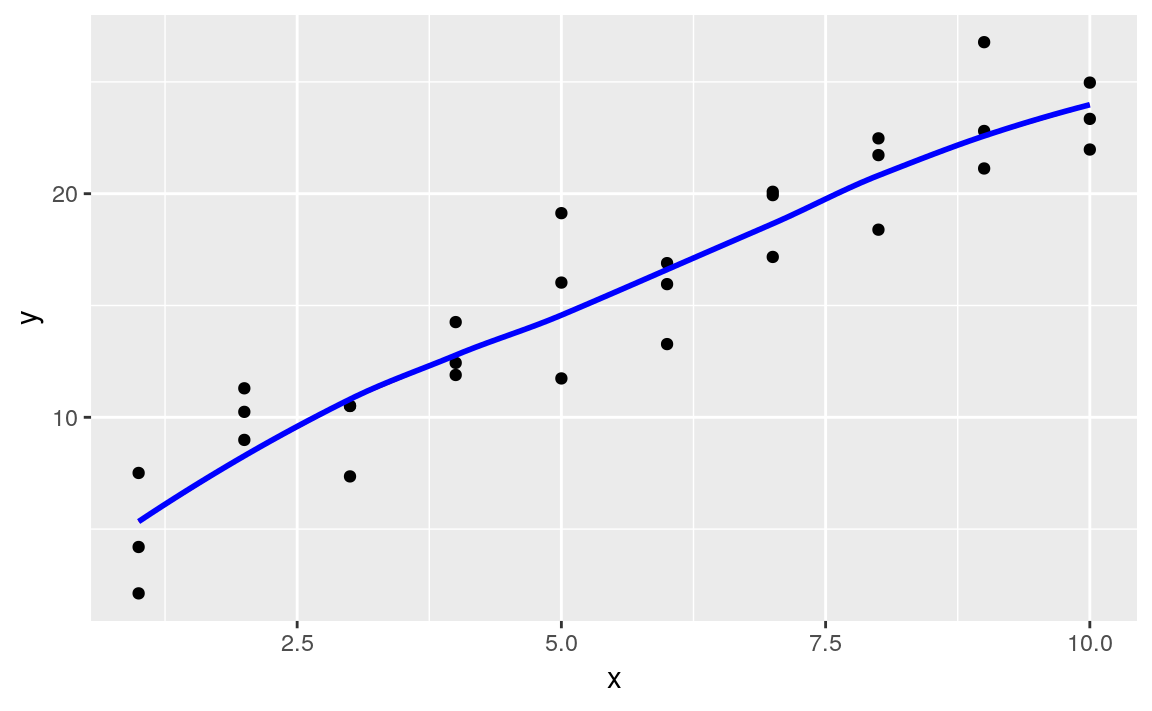
\includegraphics[width=0.7\linewidth]{visualize_files/figure-latex/unnamed-chunk-21-1} \end{center}

\hypertarget{exercise-3.6.1.3}{%
\subsection*{\texorpdfstring{Exercise
{3.6.1.3}}{Exercise 3.6.1.3}}\label{exercise-3.6.1.3}}
\addcontentsline{toc}{subsection}{Exercise {3.6.1.3}}

What does \texttt{show.legend\ =\ FALSE} do? What happens if you remove
it? Why do you think I used it earlier in the chapter?

Show legend hides the legend box. In this code, without show legend,
there is a legend.

\begin{Shaded}
\begin{Highlighting}[]
\KeywordTok{ggplot}\NormalTok{(}\DataTypeTok{data =}\NormalTok{ mpg) }\OperatorTok{+}
\StringTok{  }\KeywordTok{geom_smooth}\NormalTok{(}
    \DataTypeTok{mapping =} \KeywordTok{aes}\NormalTok{(}\DataTypeTok{x =}\NormalTok{ displ, }\DataTypeTok{y =}\NormalTok{ hwy, }\DataTypeTok{colour =}\NormalTok{ drv),}
\NormalTok{  )}
\CommentTok{#> `geom_smooth()` using method = 'loess' and formula 'y ~ x'}
\end{Highlighting}
\end{Shaded}

\begin{center}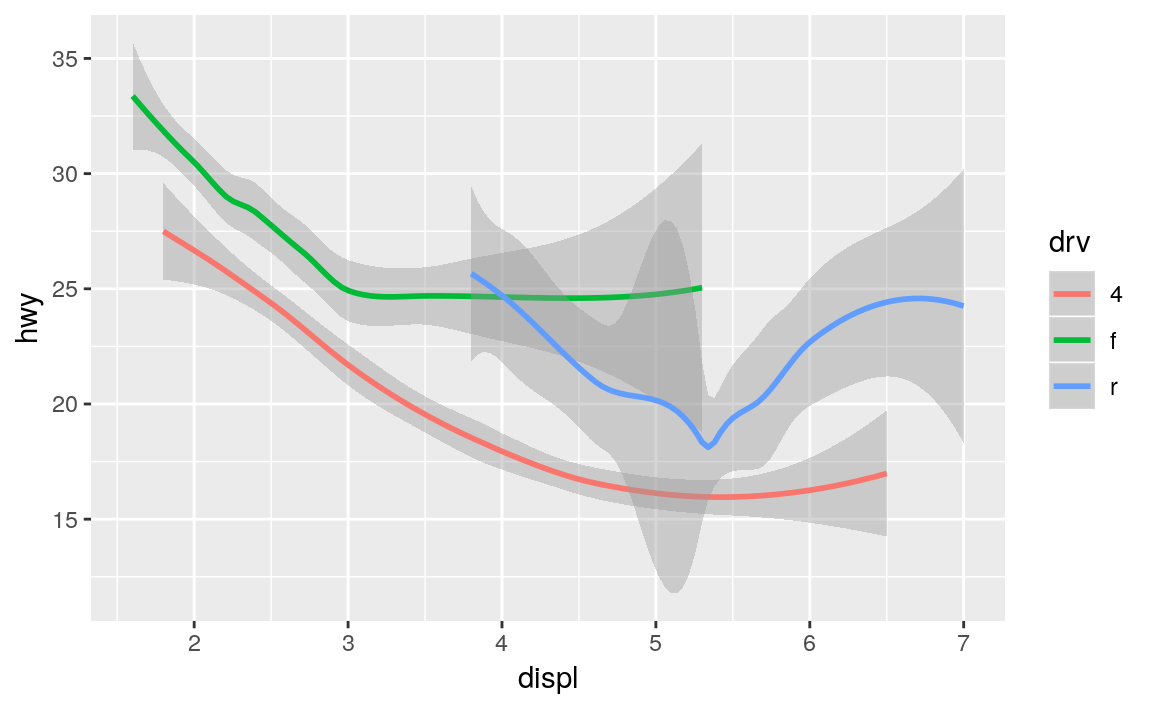
\includegraphics[width=0.7\linewidth]{visualize_files/figure-latex/unnamed-chunk-22-1} \end{center}

But there is no legend in this code:

\begin{Shaded}
\begin{Highlighting}[]
\KeywordTok{ggplot}\NormalTok{(}\DataTypeTok{data =}\NormalTok{ mpg) }\OperatorTok{+}
\StringTok{  }\KeywordTok{geom_smooth}\NormalTok{(}
    \DataTypeTok{mapping =} \KeywordTok{aes}\NormalTok{(}\DataTypeTok{x =}\NormalTok{ displ, }\DataTypeTok{y =}\NormalTok{ hwy, }\DataTypeTok{colour =}\NormalTok{ drv),}
    \DataTypeTok{show.legend =} \OtherTok{FALSE}
\NormalTok{  )}
\CommentTok{#> `geom_smooth()` using method = 'loess' and formula 'y ~ x'}
\end{Highlighting}
\end{Shaded}

\begin{center}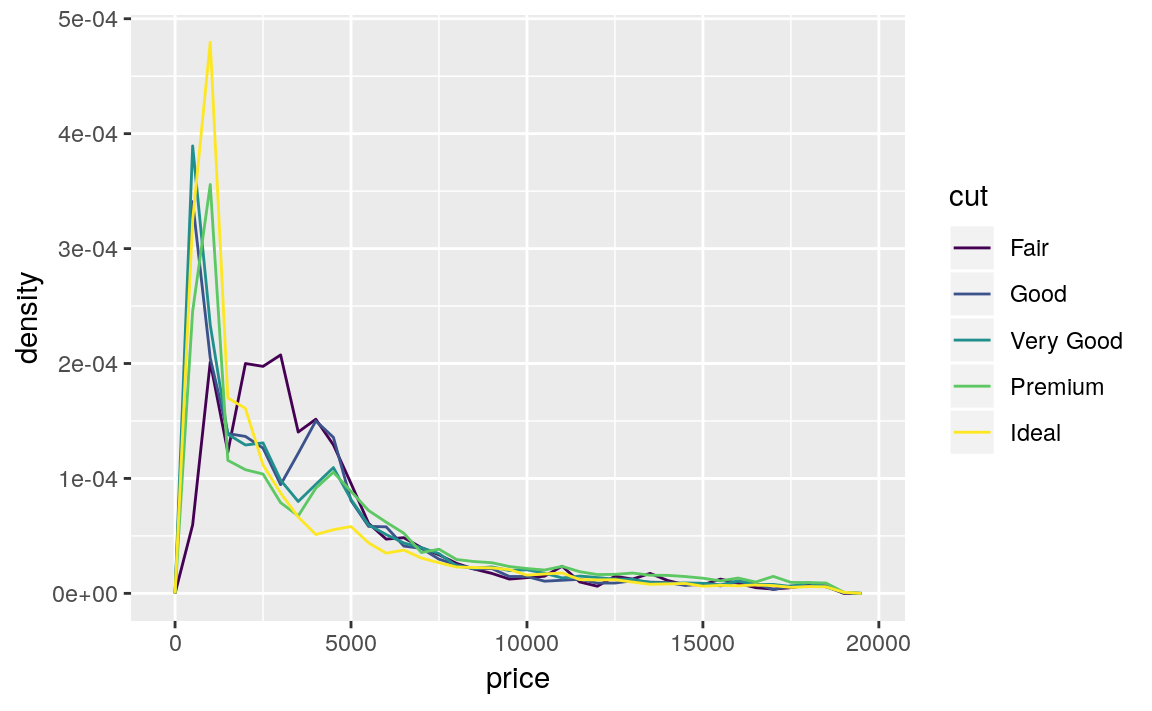
\includegraphics[width=0.7\linewidth]{visualize_files/figure-latex/unnamed-chunk-23-1} \end{center}

In the example earlier in the chapter,

\begin{Shaded}
\begin{Highlighting}[]
\KeywordTok{ggplot}\NormalTok{(}\DataTypeTok{data =}\NormalTok{ mpg) }\OperatorTok{+}
\StringTok{  }\KeywordTok{geom_smooth}\NormalTok{(}\DataTypeTok{mapping =} \KeywordTok{aes}\NormalTok{(}\DataTypeTok{x =}\NormalTok{ displ, }\DataTypeTok{y =}\NormalTok{ hwy))}
\CommentTok{#> `geom_smooth()` using method = 'loess' and formula 'y ~ x'}

\KeywordTok{ggplot}\NormalTok{(}\DataTypeTok{data =}\NormalTok{ mpg) }\OperatorTok{+}
\StringTok{  }\KeywordTok{geom_smooth}\NormalTok{(}\DataTypeTok{mapping =} \KeywordTok{aes}\NormalTok{(}\DataTypeTok{x =}\NormalTok{ displ, }\DataTypeTok{y =}\NormalTok{ hwy, }\DataTypeTok{group =}\NormalTok{ drv))}
\CommentTok{#> `geom_smooth()` using method = 'loess' and formula 'y ~ x'}

\KeywordTok{ggplot}\NormalTok{(}\DataTypeTok{data =}\NormalTok{ mpg) }\OperatorTok{+}
\StringTok{  }\KeywordTok{geom_smooth}\NormalTok{(}
    \DataTypeTok{mapping =} \KeywordTok{aes}\NormalTok{(}\DataTypeTok{x =}\NormalTok{ displ, }\DataTypeTok{y =}\NormalTok{ hwy, }\DataTypeTok{colour =}\NormalTok{ drv),}
    \DataTypeTok{show.legend =} \OtherTok{FALSE}
\NormalTok{  )}
\CommentTok{#> `geom_smooth()` using method = 'loess' and formula 'y ~ x'}
\end{Highlighting}
\end{Shaded}

\begin{center}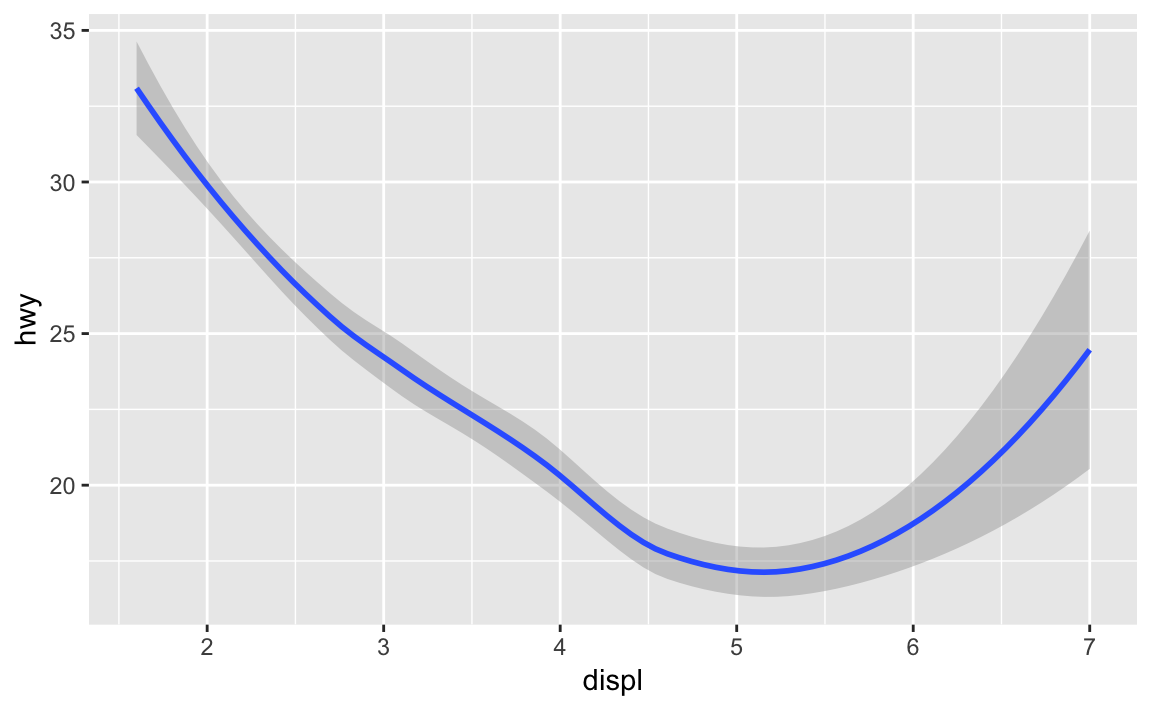
\includegraphics[width=0.7\linewidth]{visualize_files/figure-latex/unnamed-chunk-24-1} 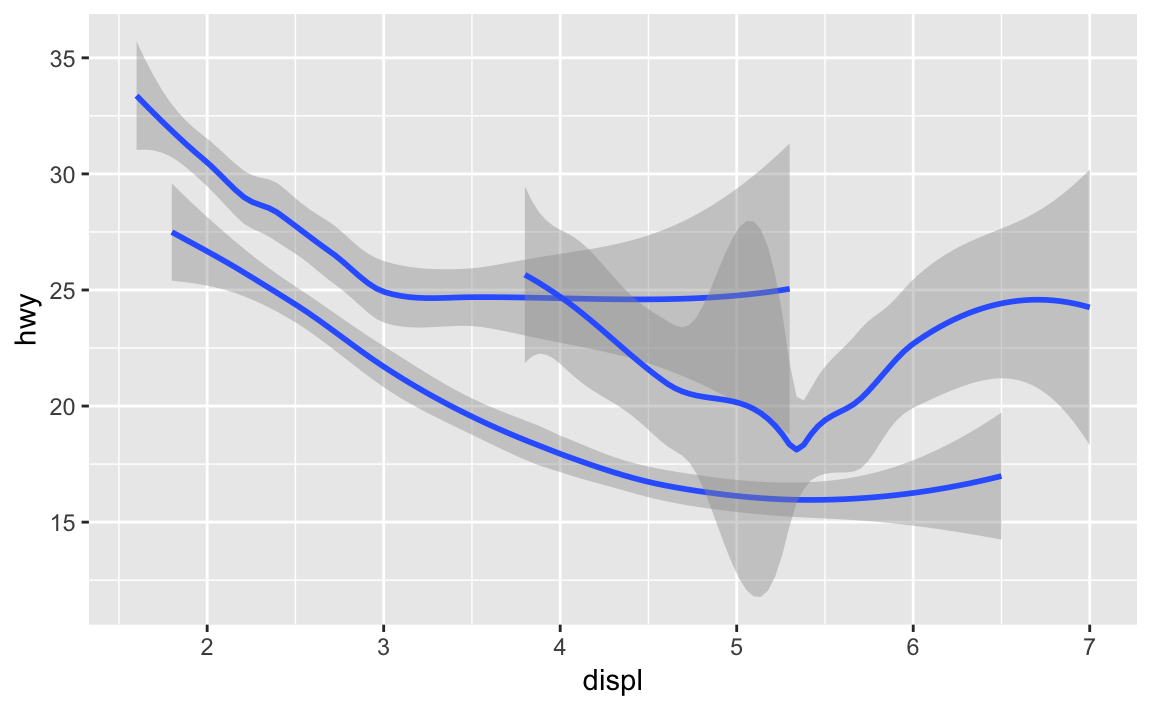
\includegraphics[width=0.7\linewidth]{visualize_files/figure-latex/unnamed-chunk-24-2} 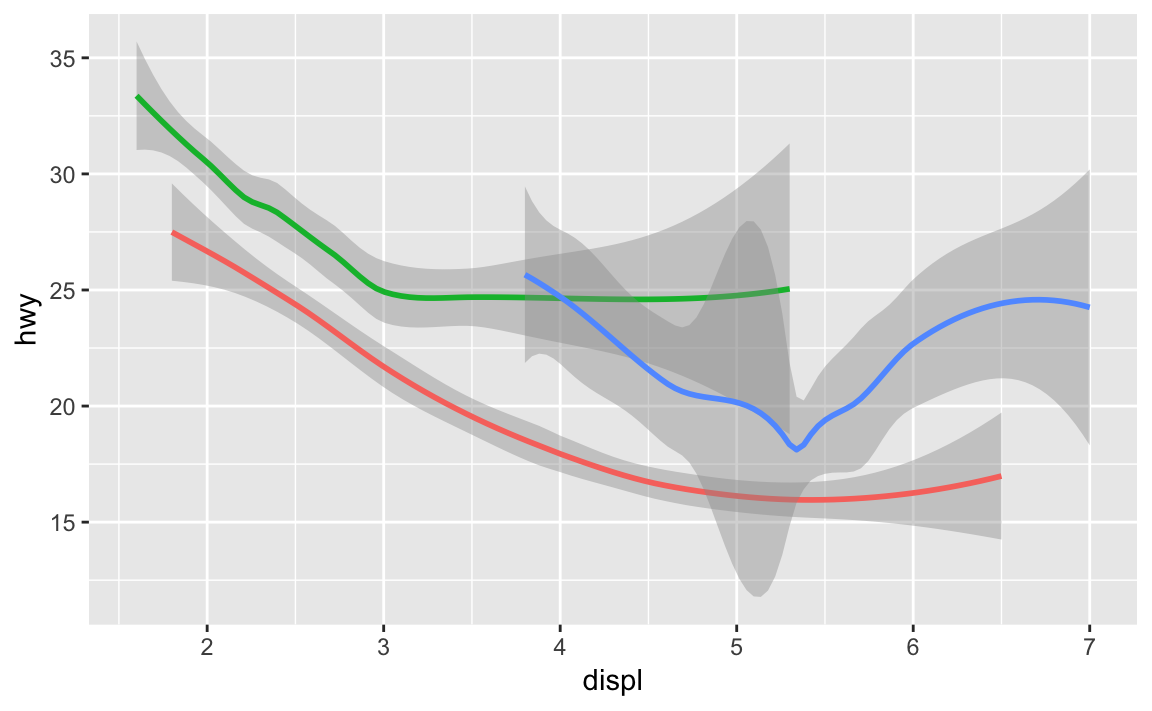
\includegraphics[width=0.7\linewidth]{visualize_files/figure-latex/unnamed-chunk-24-3} \end{center}

the legend is suppressed because there are three plots, and adding a
legend that only appears in the last one would make the presentation
asymmetric. Additionally, the purpose of this plot is to illustrate the
difference between not grouping, using a \texttt{group} aesthetic, and
using a \texttt{color} aesthetic (with implicit grouping). In that
example, the legend isn't necessary since looking up the values
associated with each color isn't necessary to make that point.

\hypertarget{exercise-3.6.1.4}{%
\subsection*{\texorpdfstring{Exercise
{3.6.1.4}}{Exercise 3.6.1.4}}\label{exercise-3.6.1.4}}
\addcontentsline{toc}{subsection}{Exercise {3.6.1.4}}

What does the \texttt{se} argument to \texttt{geom\_smooth()} do?

It adds standard error bands to the lines.

\begin{Shaded}
\begin{Highlighting}[]
\KeywordTok{ggplot}\NormalTok{(}\DataTypeTok{data =}\NormalTok{ mpg, }\DataTypeTok{mapping =} \KeywordTok{aes}\NormalTok{(}\DataTypeTok{x =}\NormalTok{ displ, }\DataTypeTok{y =}\NormalTok{ hwy, }\DataTypeTok{colour =}\NormalTok{ drv)) }\OperatorTok{+}
\StringTok{  }\KeywordTok{geom_point}\NormalTok{() }\OperatorTok{+}
\StringTok{  }\KeywordTok{geom_smooth}\NormalTok{(}\DataTypeTok{se =} \OtherTok{TRUE}\NormalTok{)}
\CommentTok{#> `geom_smooth()` using method = 'loess' and formula 'y ~ x'}
\end{Highlighting}
\end{Shaded}

\begin{center}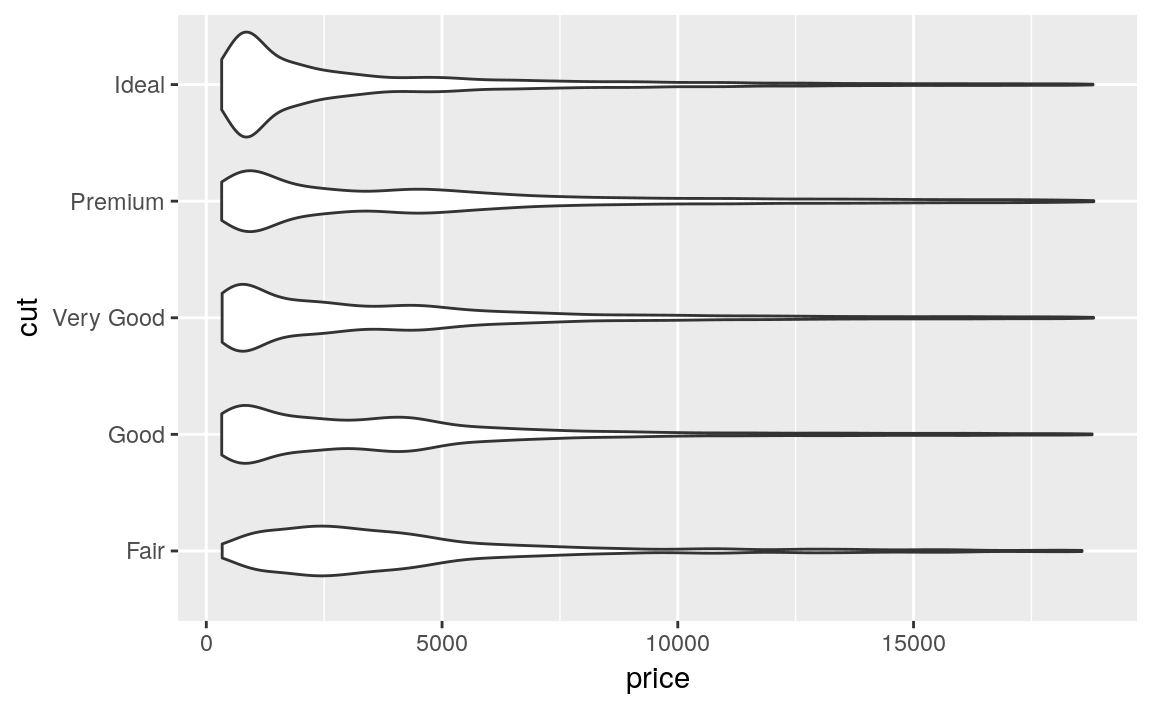
\includegraphics[width=0.7\linewidth]{visualize_files/figure-latex/unnamed-chunk-25-1} \end{center}

By default \texttt{se\ =\ TRUE}:

\begin{Shaded}
\begin{Highlighting}[]
\KeywordTok{ggplot}\NormalTok{(}\DataTypeTok{data =}\NormalTok{ mpg, }\DataTypeTok{mapping =} \KeywordTok{aes}\NormalTok{(}\DataTypeTok{x =}\NormalTok{ displ, }\DataTypeTok{y =}\NormalTok{ hwy, }\DataTypeTok{colour =}\NormalTok{ drv)) }\OperatorTok{+}
\StringTok{  }\KeywordTok{geom_point}\NormalTok{() }\OperatorTok{+}
\StringTok{  }\KeywordTok{geom_smooth}\NormalTok{()}
\CommentTok{#> `geom_smooth()` using method = 'loess' and formula 'y ~ x'}
\end{Highlighting}
\end{Shaded}

\begin{center}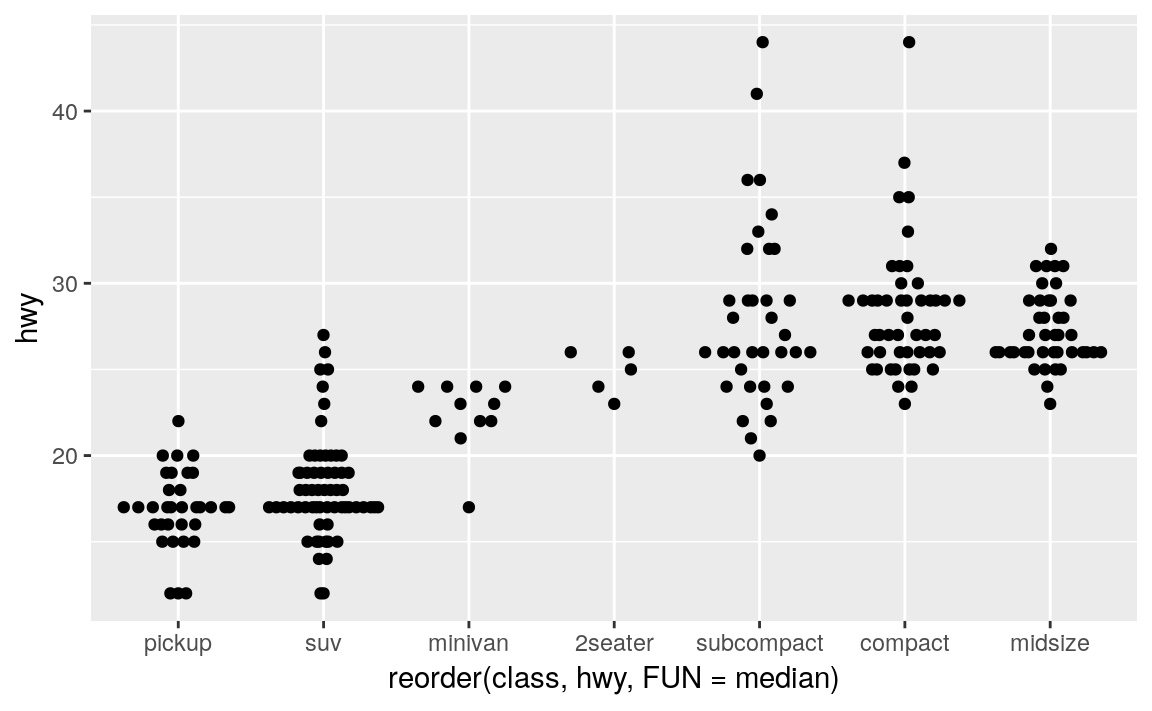
\includegraphics[width=0.7\linewidth]{visualize_files/figure-latex/unnamed-chunk-26-1} \end{center}

\hypertarget{exercise-3.6.1.5}{%
\subsection*{\texorpdfstring{Exercise
{3.6.1.5}}{Exercise 3.6.1.5}}\label{exercise-3.6.1.5}}
\addcontentsline{toc}{subsection}{Exercise {3.6.1.5}}

Will these two graphs look different? Why/why not?

No.~Because both \texttt{geom\_point()} and \texttt{geom\_smooth()} use
the same data and mappings. They will inherit those options from the
\texttt{ggplot()} object, and thus don't need to specified again (or
twice).

\begin{Shaded}
\begin{Highlighting}[]
\KeywordTok{ggplot}\NormalTok{(}\DataTypeTok{data =}\NormalTok{ mpg, }\DataTypeTok{mapping =} \KeywordTok{aes}\NormalTok{(}\DataTypeTok{x =}\NormalTok{ displ, }\DataTypeTok{y =}\NormalTok{ hwy)) }\OperatorTok{+}
\StringTok{  }\KeywordTok{geom_point}\NormalTok{() }\OperatorTok{+}
\StringTok{  }\KeywordTok{geom_smooth}\NormalTok{()}
\CommentTok{#> `geom_smooth()` using method = 'loess' and formula 'y ~ x'}
\end{Highlighting}
\end{Shaded}

\begin{center}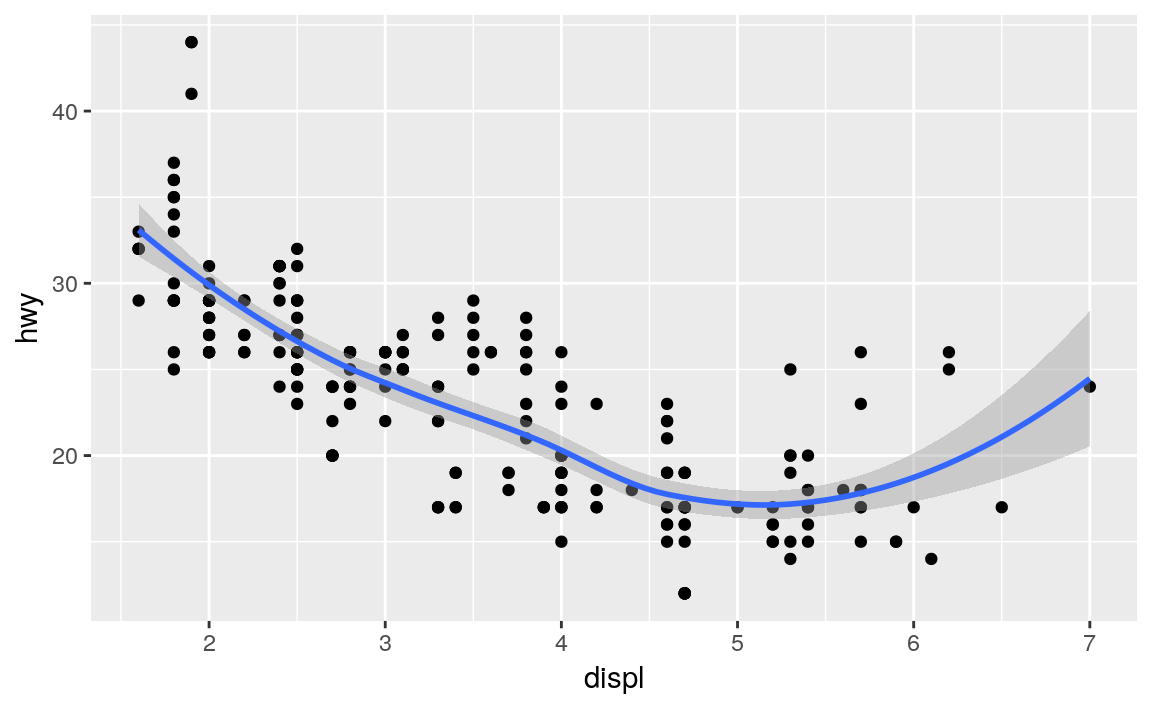
\includegraphics[width=0.7\linewidth]{visualize_files/figure-latex/unnamed-chunk-27-1} \end{center}

\begin{Shaded}
\begin{Highlighting}[]
\KeywordTok{ggplot}\NormalTok{() }\OperatorTok{+}
\StringTok{  }\KeywordTok{geom_point}\NormalTok{(}\DataTypeTok{data =}\NormalTok{ mpg, }\DataTypeTok{mapping =} \KeywordTok{aes}\NormalTok{(}\DataTypeTok{x =}\NormalTok{ displ, }\DataTypeTok{y =}\NormalTok{ hwy)) }\OperatorTok{+}
\StringTok{  }\KeywordTok{geom_smooth}\NormalTok{(}\DataTypeTok{data =}\NormalTok{ mpg, }\DataTypeTok{mapping =} \KeywordTok{aes}\NormalTok{(}\DataTypeTok{x =}\NormalTok{ displ, }\DataTypeTok{y =}\NormalTok{ hwy))}
\CommentTok{#> `geom_smooth()` using method = 'loess' and formula 'y ~ x'}
\end{Highlighting}
\end{Shaded}

\begin{center}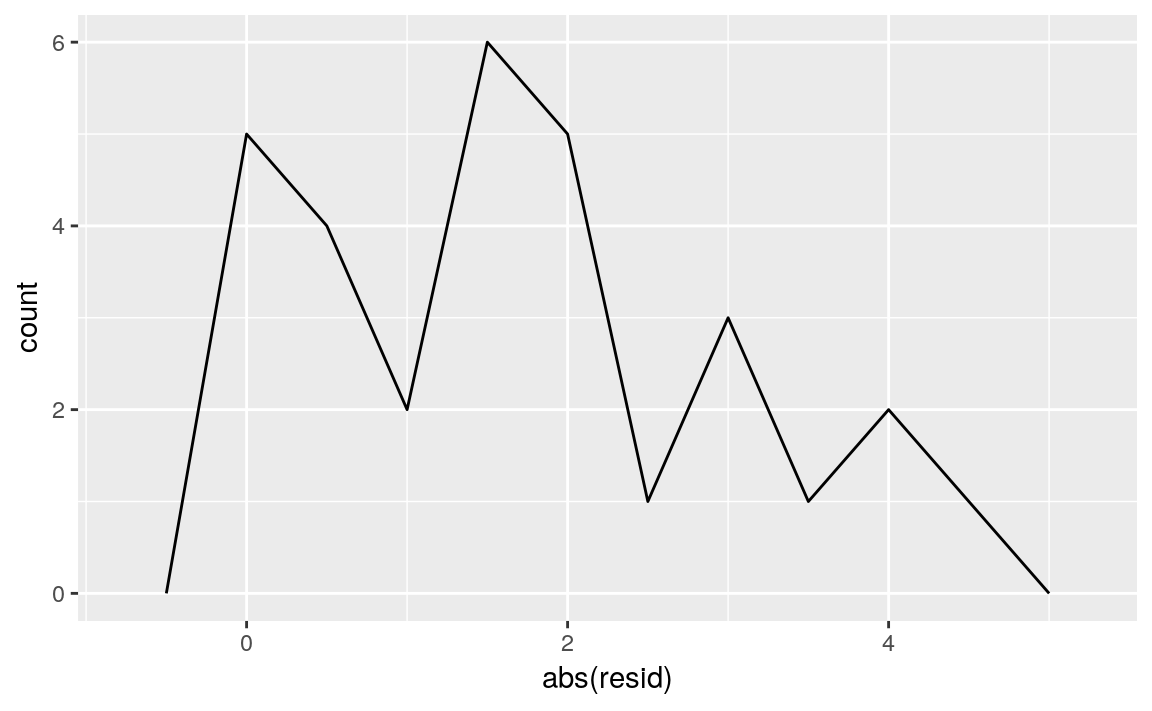
\includegraphics[width=0.7\linewidth]{visualize_files/figure-latex/unnamed-chunk-28-1} \end{center}

\hypertarget{exercise-3.6.1.6}{%
\subsection*{\texorpdfstring{Exercise
{3.6.1.6}}{Exercise 3.6.1.6}}\label{exercise-3.6.1.6}}
\addcontentsline{toc}{subsection}{Exercise {3.6.1.6}}

Recreate the R code necessary to generate the following graphs.

\begin{Shaded}
\begin{Highlighting}[]
\KeywordTok{ggplot}\NormalTok{(mpg, }\KeywordTok{aes}\NormalTok{(}\DataTypeTok{x =}\NormalTok{ displ, }\DataTypeTok{y =}\NormalTok{ hwy)) }\OperatorTok{+}
\StringTok{  }\KeywordTok{geom_point}\NormalTok{() }\OperatorTok{+}
\StringTok{  }\KeywordTok{geom_smooth}\NormalTok{(}\DataTypeTok{se =} \OtherTok{FALSE}\NormalTok{)}
\CommentTok{#> `geom_smooth()` using method = 'loess' and formula 'y ~ x'}
\end{Highlighting}
\end{Shaded}

\begin{center}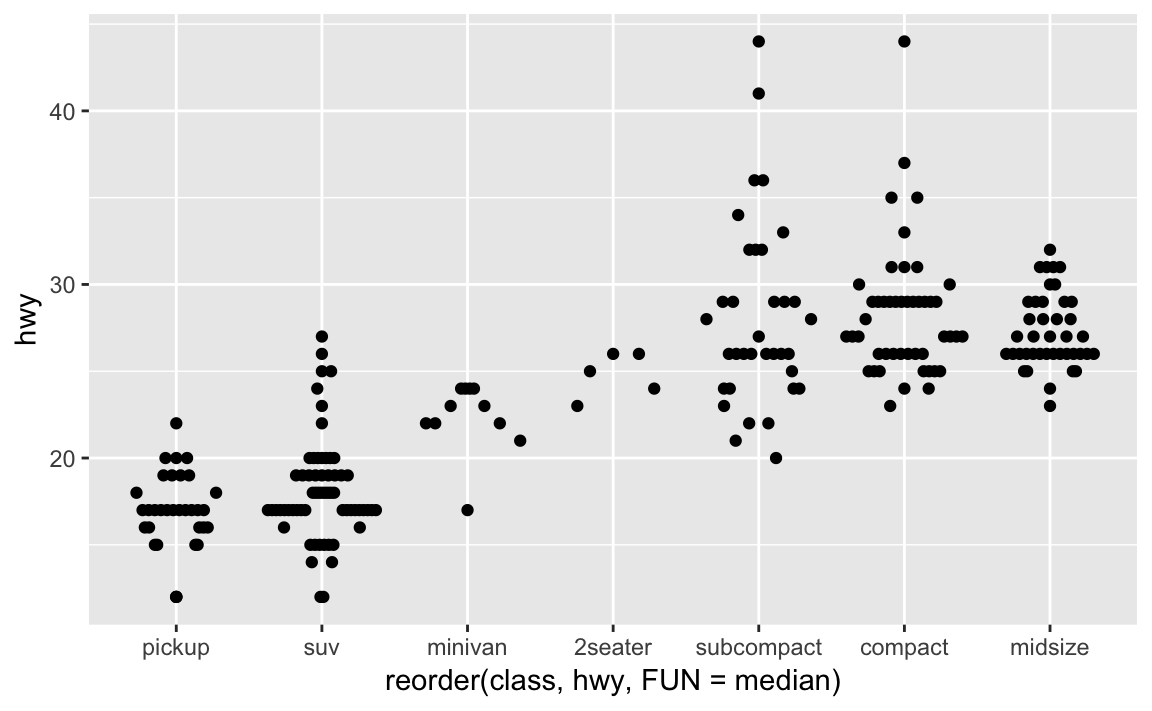
\includegraphics[width=0.7\linewidth]{visualize_files/figure-latex/unnamed-chunk-29-1} \end{center}

\begin{Shaded}
\begin{Highlighting}[]
\KeywordTok{ggplot}\NormalTok{(mpg, }\KeywordTok{aes}\NormalTok{(}\DataTypeTok{x =}\NormalTok{ displ, }\DataTypeTok{y =}\NormalTok{ hwy)) }\OperatorTok{+}
\StringTok{  }\KeywordTok{geom_smooth}\NormalTok{(}\DataTypeTok{mapping =} \KeywordTok{aes}\NormalTok{(}\DataTypeTok{group =}\NormalTok{ drv), }\DataTypeTok{se =} \OtherTok{FALSE}\NormalTok{) }\OperatorTok{+}
\StringTok{  }\KeywordTok{geom_point}\NormalTok{()}
\CommentTok{#> `geom_smooth()` using method = 'loess' and formula 'y ~ x'}
\end{Highlighting}
\end{Shaded}

\begin{center}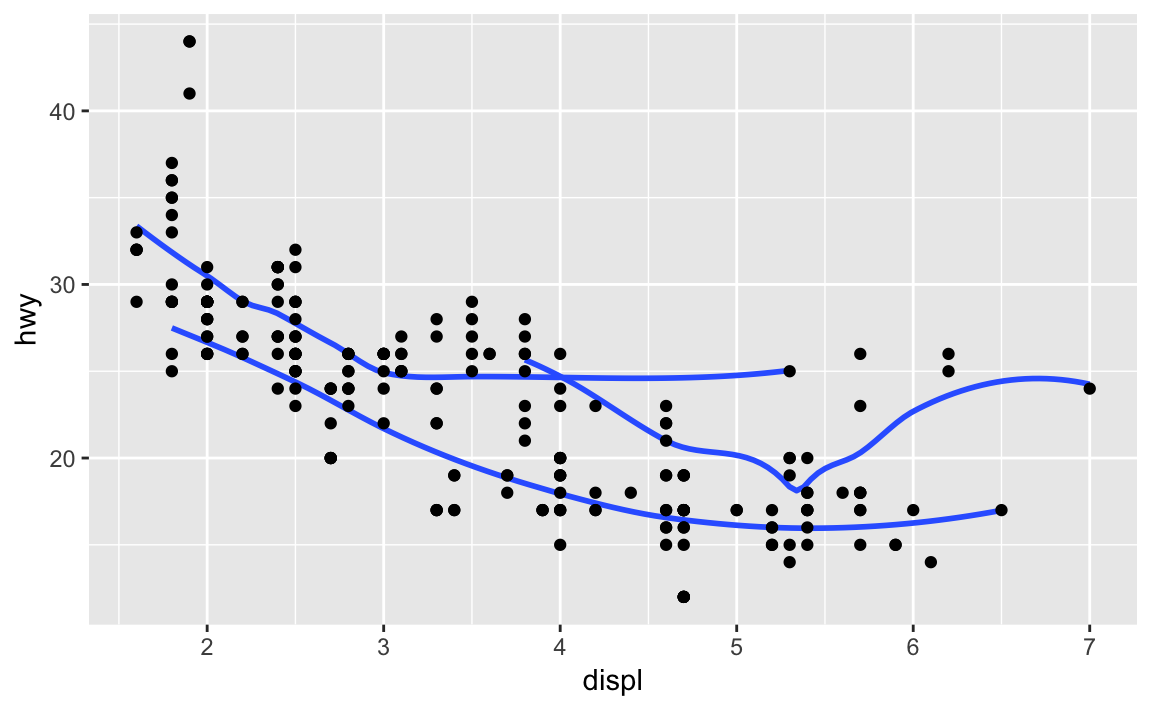
\includegraphics[width=0.7\linewidth]{visualize_files/figure-latex/unnamed-chunk-30-1} \end{center}

\begin{Shaded}
\begin{Highlighting}[]
\KeywordTok{ggplot}\NormalTok{(mpg, }\KeywordTok{aes}\NormalTok{(}\DataTypeTok{x =}\NormalTok{ displ, }\DataTypeTok{y =}\NormalTok{ hwy, }\DataTypeTok{colour =}\NormalTok{ drv)) }\OperatorTok{+}
\StringTok{  }\KeywordTok{geom_point}\NormalTok{() }\OperatorTok{+}
\StringTok{  }\KeywordTok{geom_smooth}\NormalTok{(}\DataTypeTok{se =} \OtherTok{FALSE}\NormalTok{)}
\CommentTok{#> `geom_smooth()` using method = 'loess' and formula 'y ~ x'}
\end{Highlighting}
\end{Shaded}

\begin{center}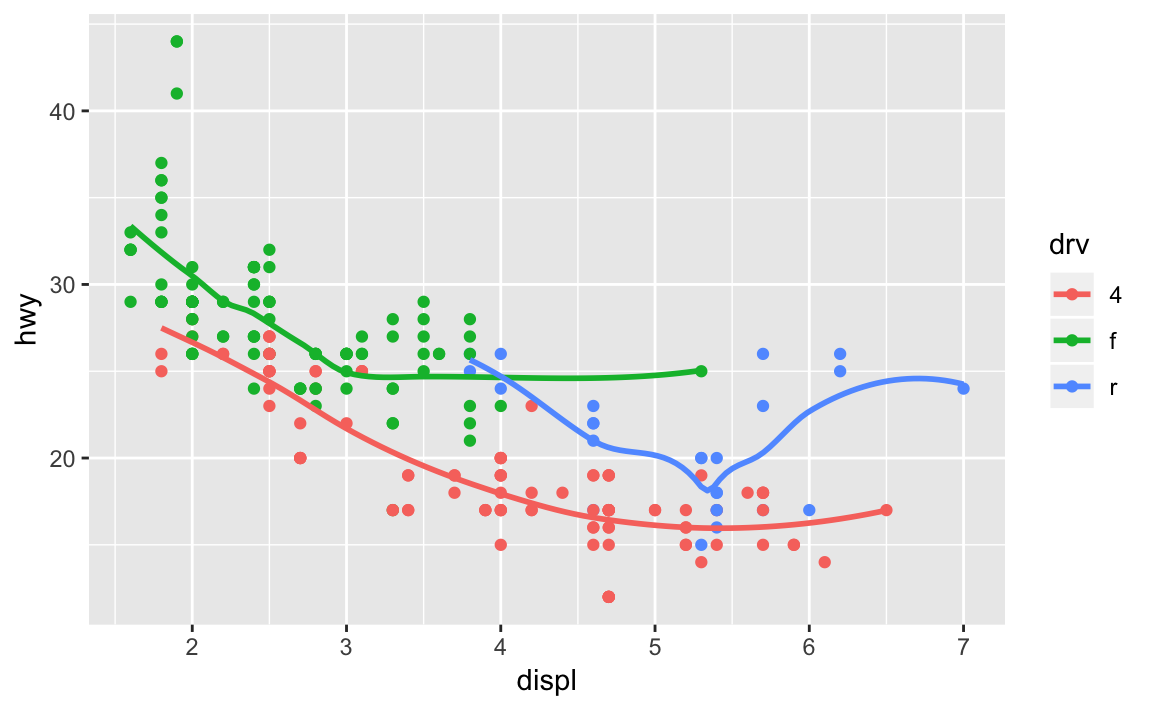
\includegraphics[width=0.7\linewidth]{visualize_files/figure-latex/unnamed-chunk-31-1} \end{center}

\begin{Shaded}
\begin{Highlighting}[]
\KeywordTok{ggplot}\NormalTok{(mpg, }\KeywordTok{aes}\NormalTok{(}\DataTypeTok{x =}\NormalTok{ displ, }\DataTypeTok{y =}\NormalTok{ hwy)) }\OperatorTok{+}
\StringTok{  }\KeywordTok{geom_point}\NormalTok{(}\KeywordTok{aes}\NormalTok{(}\DataTypeTok{colour =}\NormalTok{ drv)) }\OperatorTok{+}
\StringTok{  }\KeywordTok{geom_smooth}\NormalTok{(}\DataTypeTok{se =} \OtherTok{FALSE}\NormalTok{)}
\CommentTok{#> `geom_smooth()` using method = 'loess' and formula 'y ~ x'}
\end{Highlighting}
\end{Shaded}

\begin{center}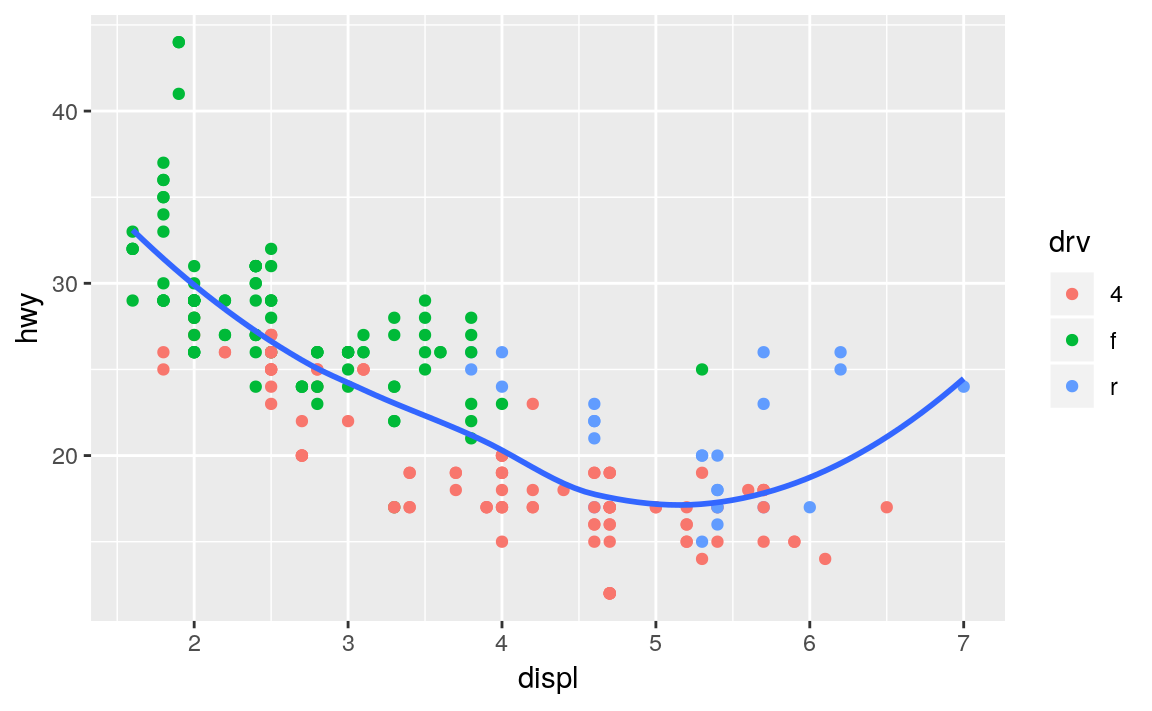
\includegraphics[width=0.7\linewidth]{visualize_files/figure-latex/unnamed-chunk-32-1} \end{center}

\begin{Shaded}
\begin{Highlighting}[]
\KeywordTok{ggplot}\NormalTok{(mpg, }\KeywordTok{aes}\NormalTok{(}\DataTypeTok{x =}\NormalTok{ displ, }\DataTypeTok{y =}\NormalTok{ hwy)) }\OperatorTok{+}
\StringTok{  }\KeywordTok{geom_point}\NormalTok{(}\KeywordTok{aes}\NormalTok{(}\DataTypeTok{colour =}\NormalTok{ drv)) }\OperatorTok{+}
\StringTok{  }\KeywordTok{geom_smooth}\NormalTok{(}\KeywordTok{aes}\NormalTok{(}\DataTypeTok{linetype =}\NormalTok{ drv), }\DataTypeTok{se =} \OtherTok{FALSE}\NormalTok{)}
\CommentTok{#> `geom_smooth()` using method = 'loess' and formula 'y ~ x'}
\end{Highlighting}
\end{Shaded}

\begin{center}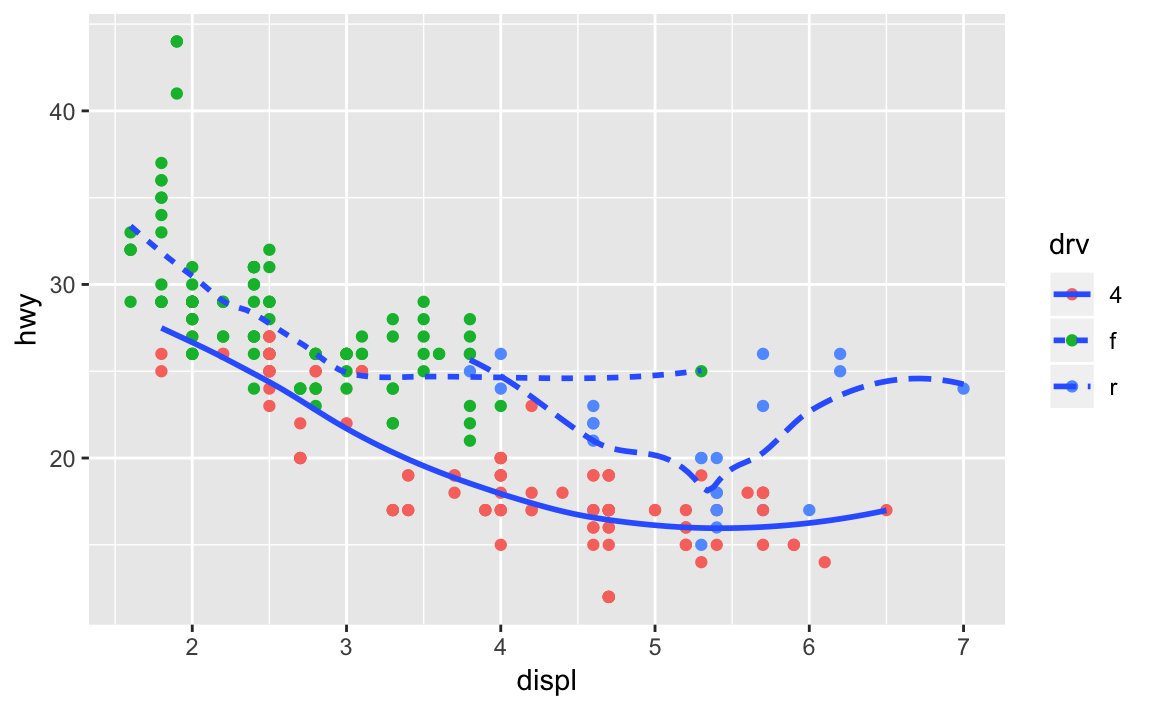
\includegraphics[width=0.7\linewidth]{visualize_files/figure-latex/unnamed-chunk-33-1} \end{center}

\begin{Shaded}
\begin{Highlighting}[]
\KeywordTok{ggplot}\NormalTok{(mpg, }\KeywordTok{aes}\NormalTok{(}\DataTypeTok{x =}\NormalTok{ displ, }\DataTypeTok{y =}\NormalTok{ hwy)) }\OperatorTok{+}
\StringTok{   }\KeywordTok{geom_point}\NormalTok{(}\DataTypeTok{size =} \DecValTok{4}\NormalTok{, }\DataTypeTok{color =} \StringTok{"white"}\NormalTok{) }\OperatorTok{+}
\StringTok{   }\KeywordTok{geom_point}\NormalTok{(}\KeywordTok{aes}\NormalTok{(}\DataTypeTok{colour =}\NormalTok{ drv))}
\end{Highlighting}
\end{Shaded}

\begin{center}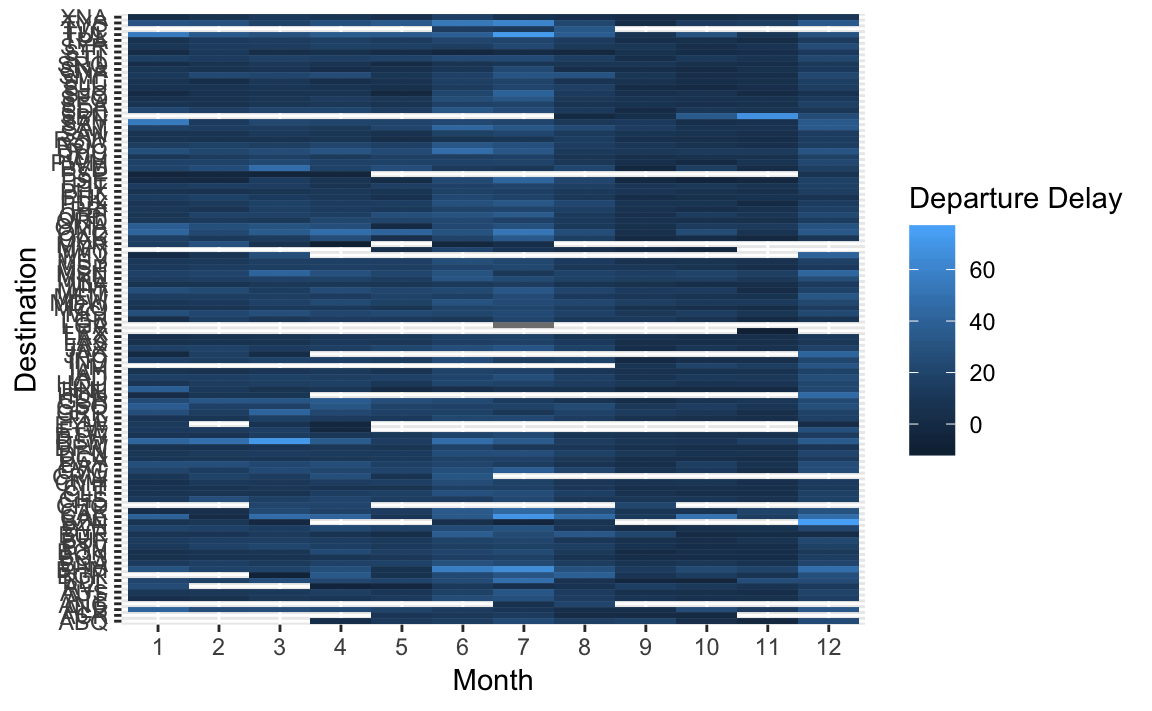
\includegraphics[width=0.7\linewidth]{visualize_files/figure-latex/unnamed-chunk-34-1} \end{center}

\hypertarget{statistical-transformations}{%
\section{Statistical
Transformations}\label{statistical-transformations}}

\hypertarget{exercise-3.7.1}{%
\subsection*{\texorpdfstring{Exercise
{3.7.1}}{Exercise 3.7.1}}\label{exercise-3.7.1}}
\addcontentsline{toc}{subsection}{Exercise {3.7.1}}

What is the default geom associated with \texttt{stat\_summary()}? How
could you rewrite the previous plot to use that geom function instead of
the stat function?

The default geom for
\href{https://ggplot2.tidyverse.org/reference/stat_summary.html}{\texttt{stat\_summary()}}
is \texttt{geom\_pointrange()} (see the \texttt{stat}) argument.

But, the default \texttt{stat} for
\href{https://ggplot2.tidyverse.org/reference/geom_linerange.html}{\texttt{geom\_pointrange()}}
is \texttt{identity()}, so use
\texttt{geom\_pointrange(stat\ =\ "summary")}.

\begin{Shaded}
\begin{Highlighting}[]
\KeywordTok{ggplot}\NormalTok{(}\DataTypeTok{data =}\NormalTok{ diamonds) }\OperatorTok{+}
\StringTok{  }\KeywordTok{geom_pointrange}\NormalTok{(}
    \DataTypeTok{mapping =} \KeywordTok{aes}\NormalTok{(}\DataTypeTok{x =}\NormalTok{ cut, }\DataTypeTok{y =}\NormalTok{ depth),}
    \DataTypeTok{stat =} \StringTok{"summary"}\NormalTok{,}
\NormalTok{  )}
\CommentTok{#> No summary function supplied, defaulting to `mean_se()}
\end{Highlighting}
\end{Shaded}

\begin{center}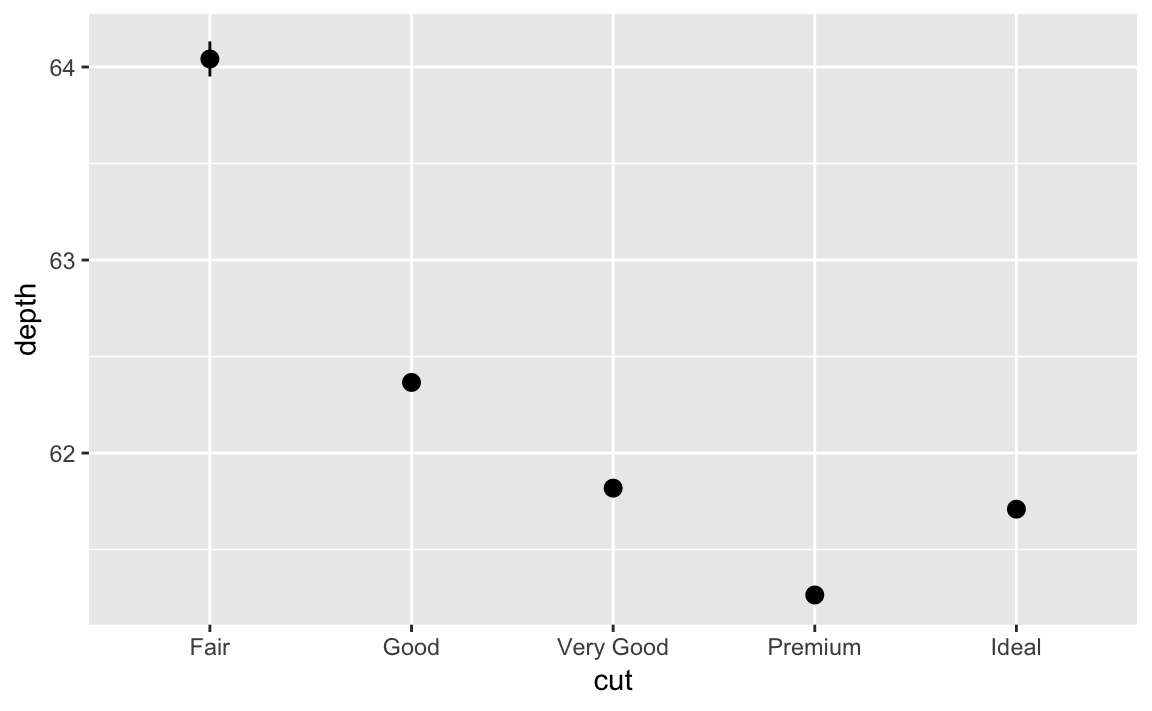
\includegraphics[width=0.7\linewidth]{visualize_files/figure-latex/unnamed-chunk-35-1} \end{center}

The default message says that \texttt{stat\_summary()} uses the
\texttt{mean} and \texttt{sd} to calculate the point, and range of the
line. So lets use the previous values of \texttt{fun.ymin},
\texttt{fun.ymax}, and \texttt{fun.y}:

\begin{Shaded}
\begin{Highlighting}[]
\KeywordTok{ggplot}\NormalTok{(}\DataTypeTok{data =}\NormalTok{ diamonds) }\OperatorTok{+}
\StringTok{  }\KeywordTok{geom_pointrange}\NormalTok{(}
    \DataTypeTok{mapping =} \KeywordTok{aes}\NormalTok{(}\DataTypeTok{x =}\NormalTok{ cut, }\DataTypeTok{y =}\NormalTok{ depth),}
    \DataTypeTok{stat =} \StringTok{"summary"}\NormalTok{,}
    \DataTypeTok{fun.ymin =}\NormalTok{ min,}
    \DataTypeTok{fun.ymax =}\NormalTok{ max,}
    \DataTypeTok{fun.y =}\NormalTok{ median}
\NormalTok{  )}
\end{Highlighting}
\end{Shaded}

\begin{center}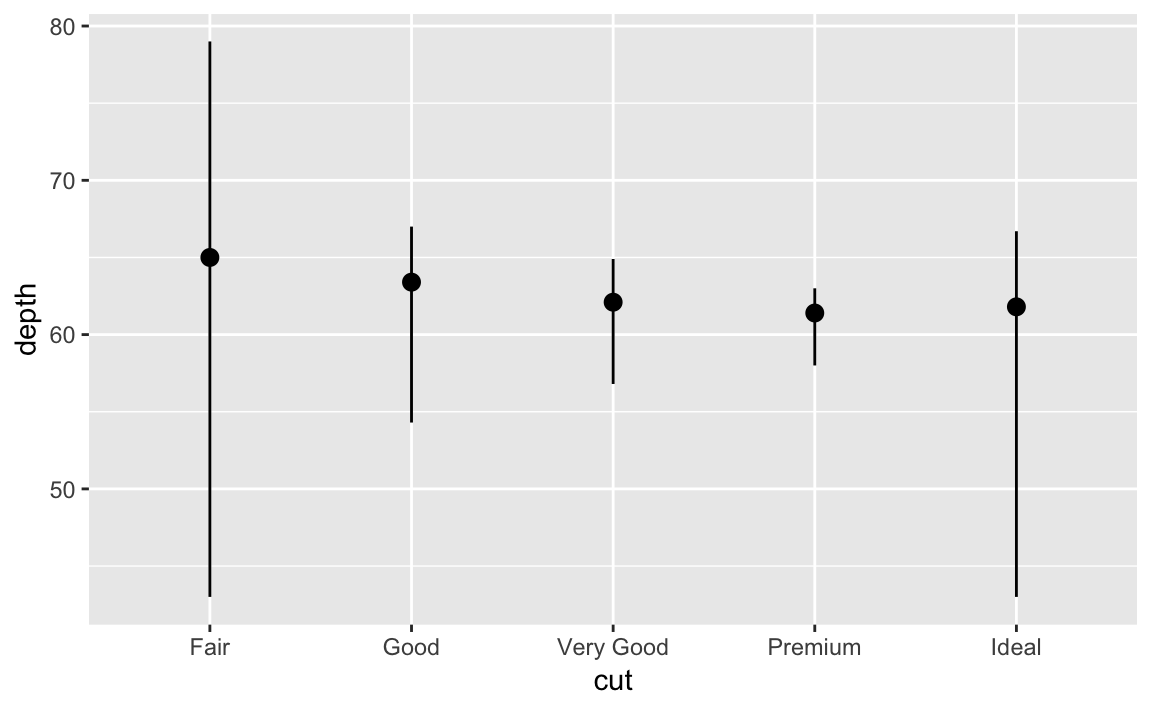
\includegraphics[width=0.7\linewidth]{visualize_files/figure-latex/unnamed-chunk-36-1} \end{center}

\hypertarget{exercise-3.7.2.}{%
\subsection*{\texorpdfstring{Exercise
{3.7.2}.}{Exercise 3.7.2.}}\label{exercise-3.7.2.}}
\addcontentsline{toc}{subsection}{Exercise {3.7.2}.}

What does \texttt{geom\_col()} do? How is it different to
\texttt{geom\_bar()}?

The \texttt{geom\_col()} function has different default than
\texttt{geom\_bar()}. The default stat of
\texttt{geom\_col()\ is}identity()\texttt{stat.\ This\ means\ that}geom\_col()\texttt{expects\ that\ the\ data\ is\ already\ preprocessed\ into}x\texttt{values\ and}y\texttt{values\ representing\ the\ bar\ height.\ The\ defult\ stat\ of}geom\_bar()\texttt{is}count()\texttt{.\ This\ means\ that}geom\_bar()\texttt{expects\ the}x\texttt{variable\ to\ contain\ multiple\ observations\ for\ each\ values,\ and\ it\ will\ handle\ counting\ the\ number\ of\ observations\ for\ each\ value\ of}x`
in order to create the bar heights.

\hypertarget{exercise-3.7.3.}{%
\subsection*{\texorpdfstring{Exercise
{3.7.3}.}{Exercise 3.7.3.}}\label{exercise-3.7.3.}}
\addcontentsline{toc}{subsection}{Exercise {3.7.3}.}

Most geoms and stats come in pairs that are almost always used in
concert. Read through the documentation and make a list of all the
pairs. What do they have in common?

See the \href{https://ggplot2.tidyverse.org/reference/}{ggplot2
documentation}.

\textbf{TODO}

\hypertarget{exercise-3.7.4.}{%
\subsection*{\texorpdfstring{Exercise
{3.7.4}.}{Exercise 3.7.4.}}\label{exercise-3.7.4.}}
\addcontentsline{toc}{subsection}{Exercise {3.7.4}.}

What variables does \texttt{stat\_smooth()} compute? What parameters
control its behavior?

The function \texttt{stat\_smooth()} calculates the following
statistics:

\begin{itemize}
\tightlist
\item
  \texttt{y}: predicted value
\item
  \texttt{ymin}: lower value of the confidence interval
\item
  \texttt{ymax}: upper value of the confidence interval
\item
  \texttt{se}: standard error
\end{itemize}

There's parameters such as \texttt{method} which determines which method
is used to calculate the predictions and confidence interval, and some
other arguments that are passed to that.

\hypertarget{exercise-3.7.5.}{%
\subsection*{\texorpdfstring{Exercise
{3.7.5}.}{Exercise 3.7.5.}}\label{exercise-3.7.5.}}
\addcontentsline{toc}{subsection}{Exercise {3.7.5}.}

In our proportion bar chart, we need to set \texttt{group\ =\ 1} Why? In
other words what is the problem with these two graphs?

If \texttt{group} is not set to 1, then all the bars have
\texttt{prop\ ==\ 1}. The function \texttt{geom\_bar()} assumes that the
groups are equal to the \texttt{x} values, since the stat computes the
counts within the group.

\begin{Shaded}
\begin{Highlighting}[]
\KeywordTok{ggplot}\NormalTok{(}\DataTypeTok{data =}\NormalTok{ diamonds) }\OperatorTok{+}
\StringTok{  }\KeywordTok{geom_bar}\NormalTok{(}\DataTypeTok{mapping =} \KeywordTok{aes}\NormalTok{(}\DataTypeTok{x =}\NormalTok{ cut, }\DataTypeTok{y =}\NormalTok{ ..prop..))}
\end{Highlighting}
\end{Shaded}

\begin{center}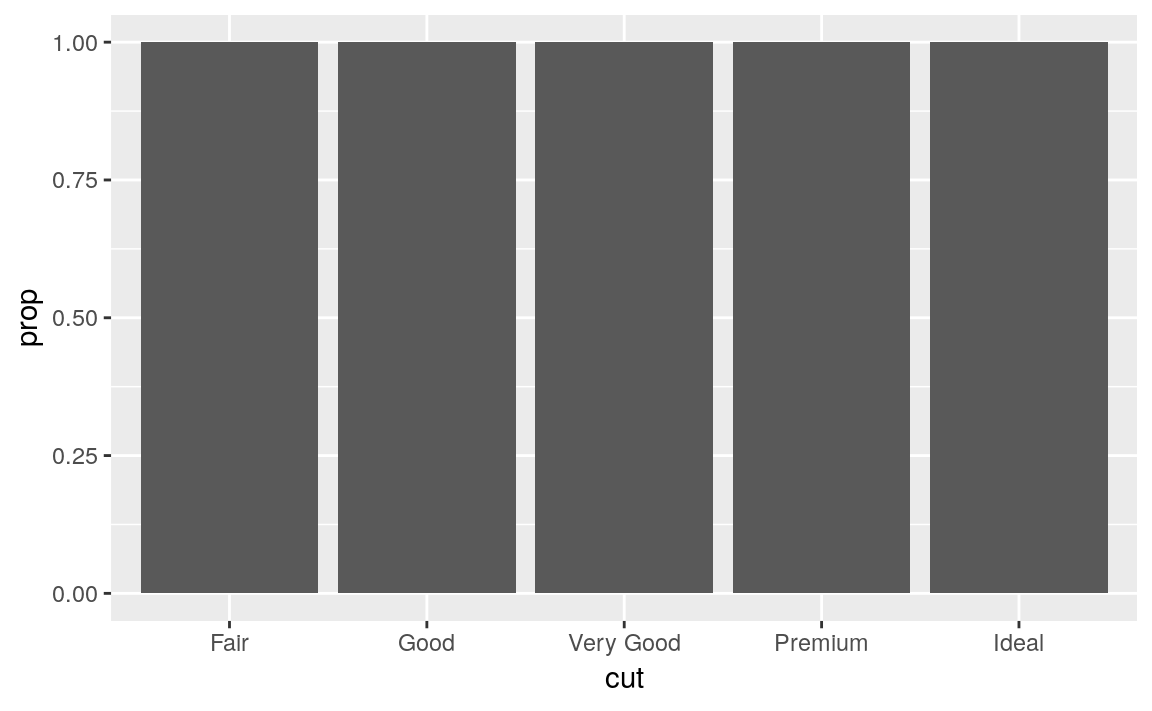
\includegraphics[width=0.7\linewidth]{visualize_files/figure-latex/unnamed-chunk-37-1} \end{center}

The problem with these two plots is that the proportions are calculated
within the groups.

\begin{Shaded}
\begin{Highlighting}[]
\KeywordTok{ggplot}\NormalTok{(}\DataTypeTok{data =}\NormalTok{ diamonds) }\OperatorTok{+}
\StringTok{  }\KeywordTok{geom_bar}\NormalTok{(}\DataTypeTok{mapping =} \KeywordTok{aes}\NormalTok{(}\DataTypeTok{x =}\NormalTok{ cut, }\DataTypeTok{y =}\NormalTok{ ..prop..))}

\KeywordTok{ggplot}\NormalTok{(}\DataTypeTok{data =}\NormalTok{ diamonds) }\OperatorTok{+}
\StringTok{  }\KeywordTok{geom_bar}\NormalTok{(}\DataTypeTok{mapping =} \KeywordTok{aes}\NormalTok{(}\DataTypeTok{x =}\NormalTok{ cut, }\DataTypeTok{fill =}\NormalTok{ color, }\DataTypeTok{y =}\NormalTok{ ..prop..))}
\end{Highlighting}
\end{Shaded}

\begin{center}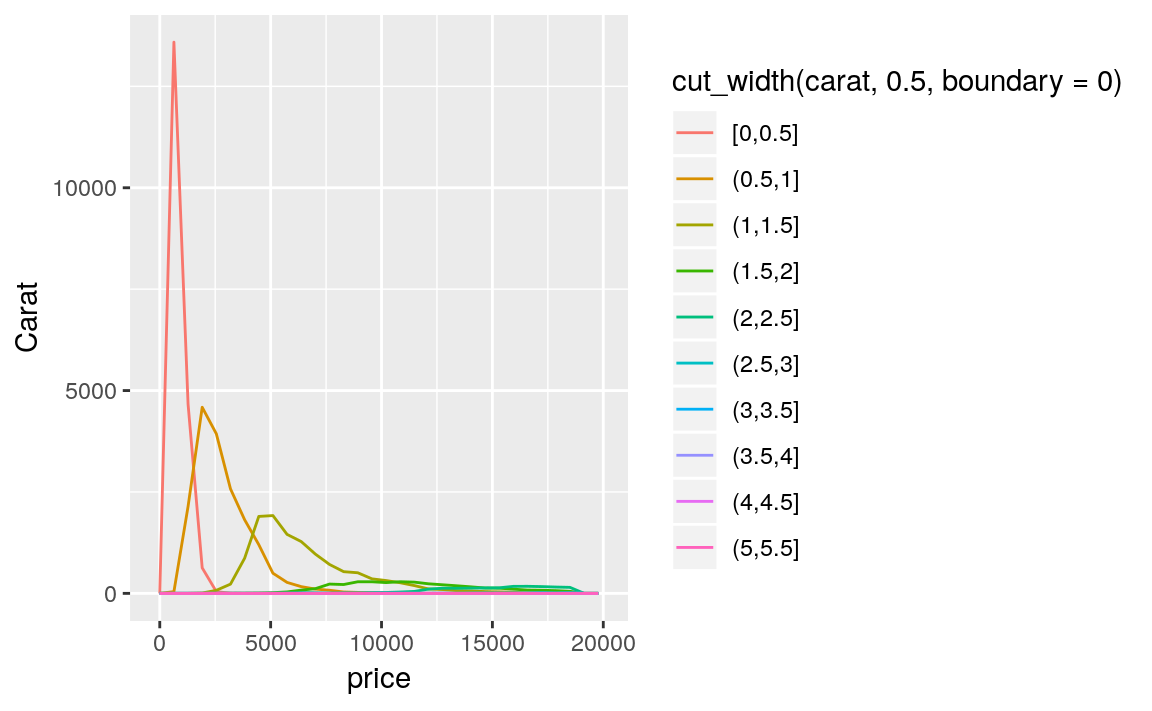
\includegraphics[width=0.7\linewidth]{visualize_files/figure-latex/unnamed-chunk-38-1} 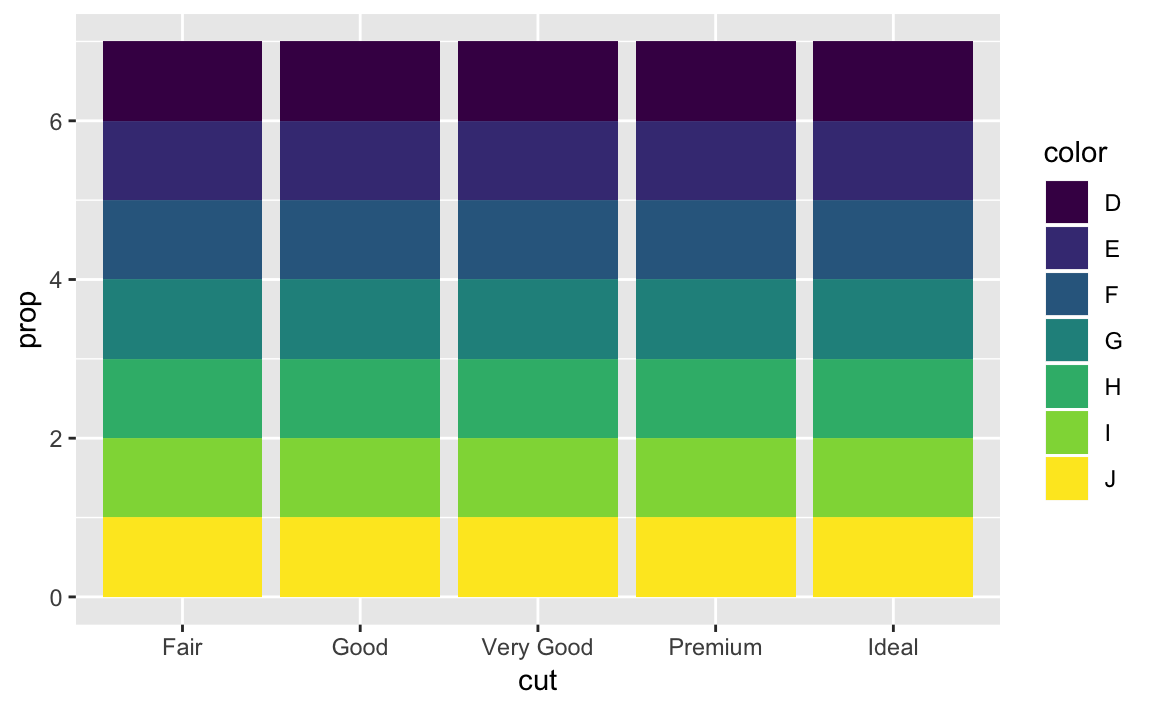
\includegraphics[width=0.7\linewidth]{visualize_files/figure-latex/unnamed-chunk-38-2} \end{center}

This is more likely what was intended:

\begin{Shaded}
\begin{Highlighting}[]
\KeywordTok{ggplot}\NormalTok{(}\DataTypeTok{data =}\NormalTok{ diamonds) }\OperatorTok{+}
\StringTok{  }\KeywordTok{geom_bar}\NormalTok{(}\DataTypeTok{mapping =} \KeywordTok{aes}\NormalTok{(}\DataTypeTok{x =}\NormalTok{ cut, }\DataTypeTok{y =}\NormalTok{ ..prop.., }\DataTypeTok{group =} \DecValTok{1}\NormalTok{))}

\KeywordTok{ggplot}\NormalTok{(}\DataTypeTok{data =}\NormalTok{ diamonds) }\OperatorTok{+}
\StringTok{  }\KeywordTok{geom_bar}\NormalTok{(}\DataTypeTok{mapping =} \KeywordTok{aes}\NormalTok{(}\DataTypeTok{x =}\NormalTok{ cut, }\DataTypeTok{fill =}\NormalTok{ color, }\DataTypeTok{y =}\NormalTok{ ..prop.., }\DataTypeTok{group =}\NormalTok{ color))}
\end{Highlighting}
\end{Shaded}

\begin{center}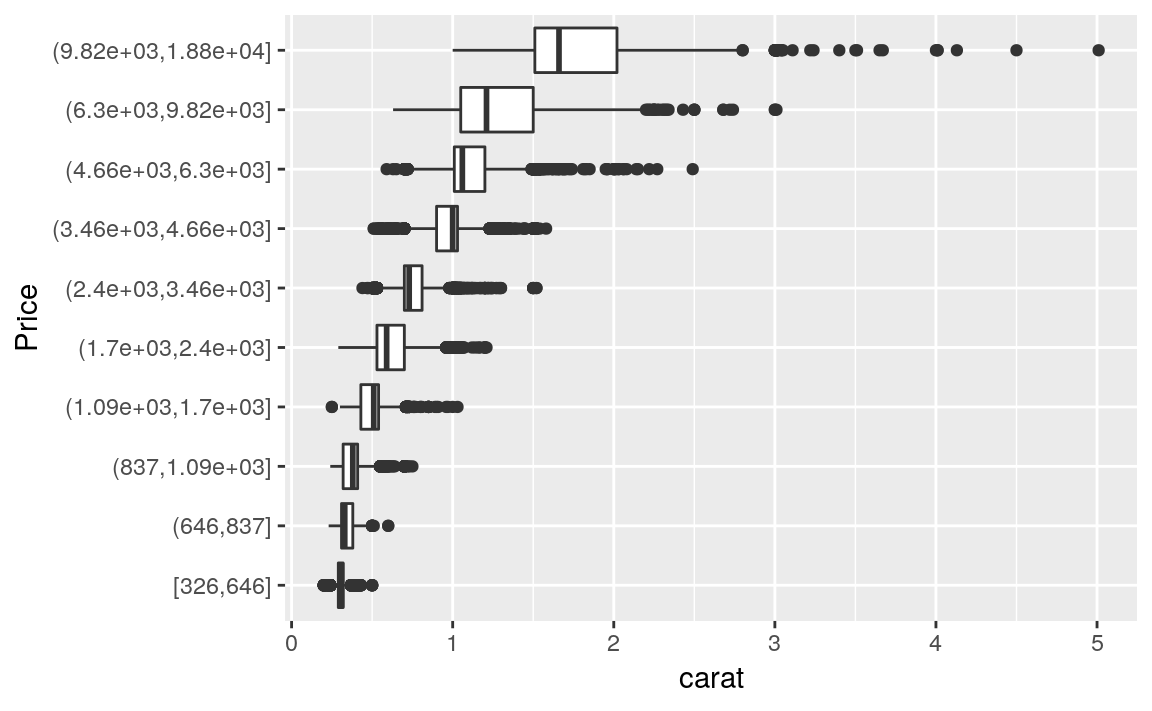
\includegraphics[width=0.7\linewidth]{visualize_files/figure-latex/unnamed-chunk-39-1} 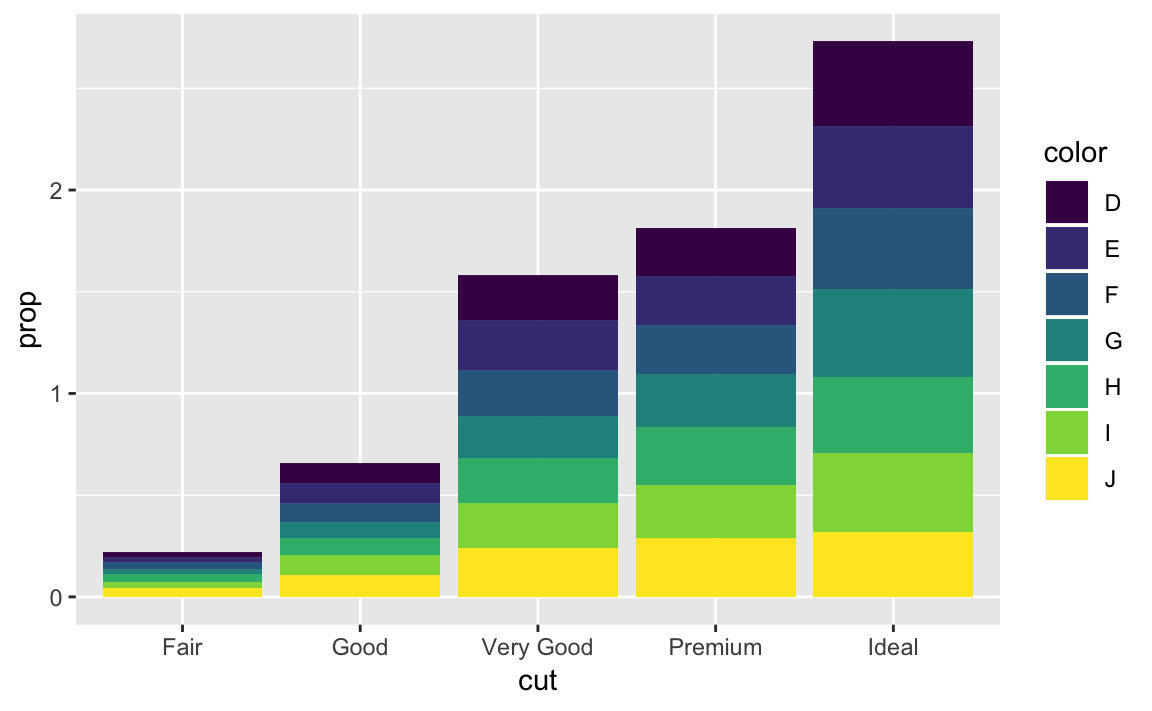
\includegraphics[width=0.7\linewidth]{visualize_files/figure-latex/unnamed-chunk-39-2} \end{center}

\hypertarget{position-adjustments}{%
\section{Position Adjustments}\label{position-adjustments}}

\hypertarget{exercise-3.8.1.1.}{%
\subsection*{\texorpdfstring{Exercise
{3.8.1.1}.}{Exercise 3.8.1.1.}}\label{exercise-3.8.1.1.}}
\addcontentsline{toc}{subsection}{Exercise {3.8.1.1}.}

What is the problem with this plot? How could you improve it?

There is overplotting because there are multiple observations for each
combination of \texttt{cty} and \texttt{hwy}.

\begin{Shaded}
\begin{Highlighting}[]
\KeywordTok{ggplot}\NormalTok{(}\DataTypeTok{data =}\NormalTok{ mpg, }\DataTypeTok{mapping =} \KeywordTok{aes}\NormalTok{(}\DataTypeTok{x =}\NormalTok{ cty, }\DataTypeTok{y =}\NormalTok{ hwy)) }\OperatorTok{+}
\StringTok{  }\KeywordTok{geom_point}\NormalTok{()}
\end{Highlighting}
\end{Shaded}

\begin{center}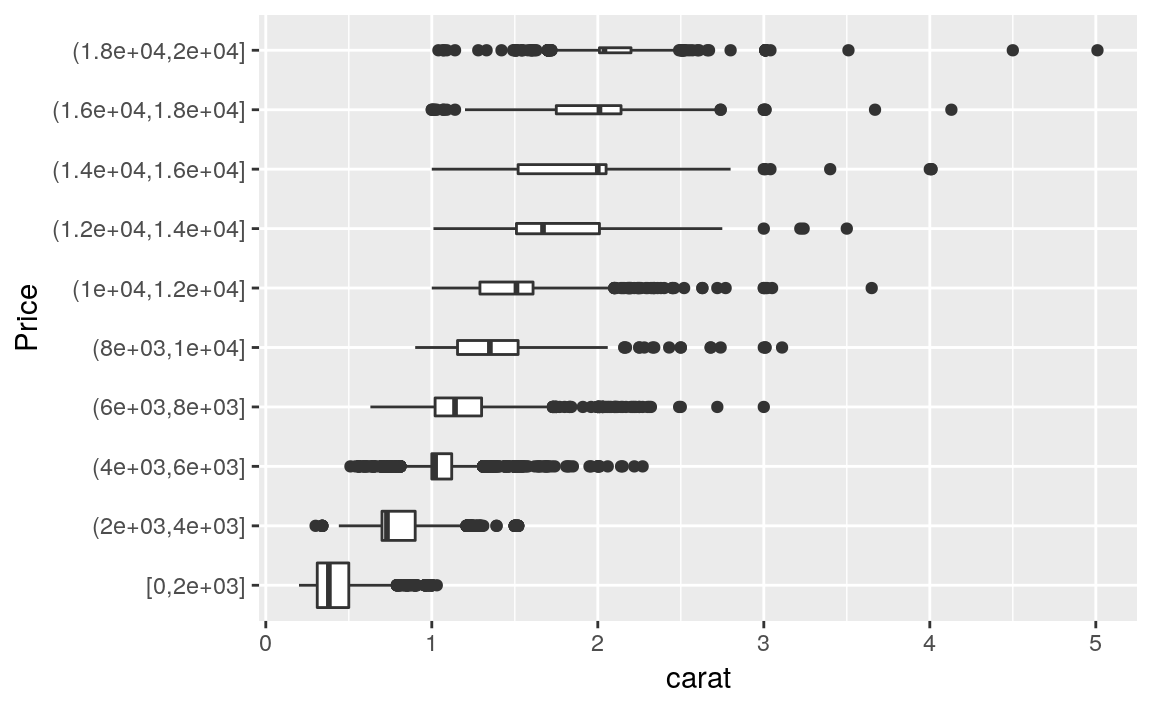
\includegraphics[width=0.7\linewidth]{visualize_files/figure-latex/unnamed-chunk-40-1} \end{center}

I'd fix it by using a jitter position adjustment.

\begin{Shaded}
\begin{Highlighting}[]
\KeywordTok{ggplot}\NormalTok{(}\DataTypeTok{data =}\NormalTok{ mpg, }\DataTypeTok{mapping =} \KeywordTok{aes}\NormalTok{(}\DataTypeTok{x =}\NormalTok{ cty, }\DataTypeTok{y =}\NormalTok{ hwy)) }\OperatorTok{+}
\StringTok{  }\KeywordTok{geom_point}\NormalTok{(}\DataTypeTok{position =} \StringTok{"jitter"}\NormalTok{)}
\end{Highlighting}
\end{Shaded}

\begin{center}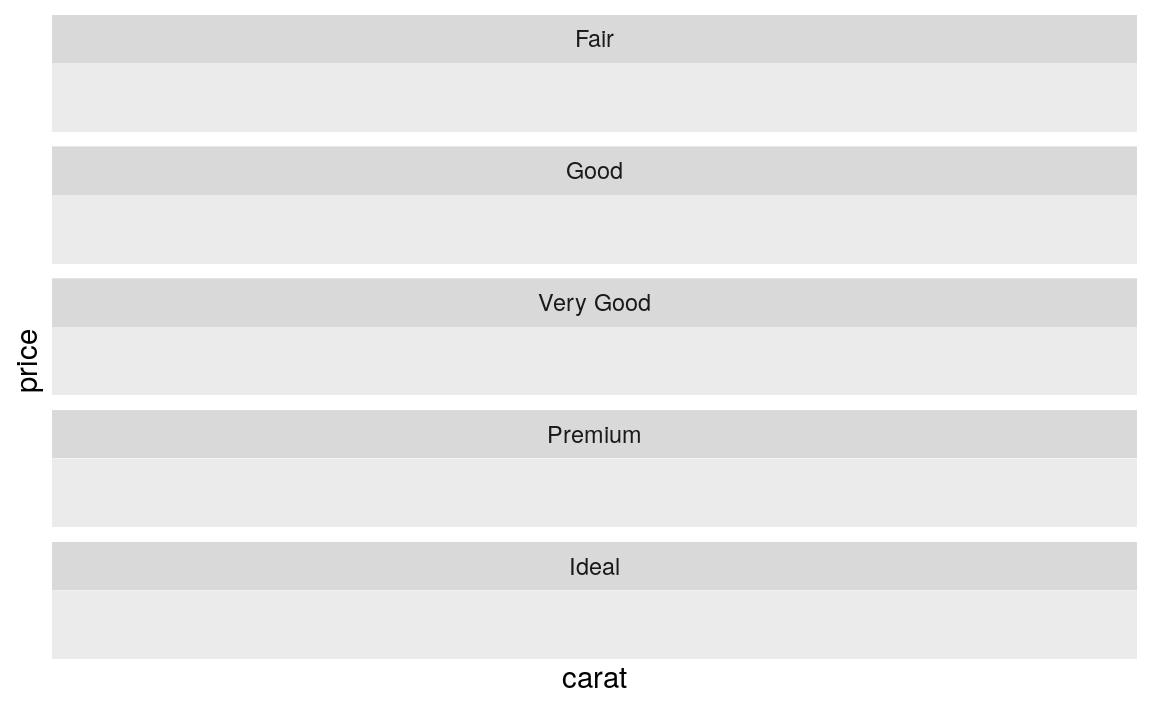
\includegraphics[width=0.7\linewidth]{visualize_files/figure-latex/unnamed-chunk-41-1} \end{center}

\hypertarget{exercise-3.8.1.2.}{%
\subsection*{\texorpdfstring{Exercise
{3.8.1.2}.}{Exercise 3.8.1.2.}}\label{exercise-3.8.1.2.}}
\addcontentsline{toc}{subsection}{Exercise {3.8.1.2}.}

What parameters to \texttt{geom\_jitter()} control the amount of
jittering?

From the
\href{https://ggplot2.tidyverse.org/reference/geom_jitter.html}{\texttt{geom\_jitter()}}
documentation, there are two arguments to jitter:

\begin{itemize}
\tightlist
\item
  \texttt{width} controls the amount of vertical displacement, and
\item
  \texttt{height} controls the amount of horizontal displacement.
\end{itemize}

The defaults values of \texttt{width} and \texttt{height} will introduce
noise in both directions. Here is what the plot looks like with the
default values of \texttt{height} and \texttt{width}.

\begin{Shaded}
\begin{Highlighting}[]
\KeywordTok{ggplot}\NormalTok{(}\DataTypeTok{data =}\NormalTok{ mpg, }\DataTypeTok{mapping =} \KeywordTok{aes}\NormalTok{(}\DataTypeTok{x =}\NormalTok{ cty, }\DataTypeTok{y =}\NormalTok{ hwy)) }\OperatorTok{+}
\StringTok{  }\KeywordTok{geom_point}\NormalTok{(}\DataTypeTok{position =} \KeywordTok{position_jitter}\NormalTok{(}\DataTypeTok{width =} \DecValTok{0}\NormalTok{))}
\end{Highlighting}
\end{Shaded}

\begin{center}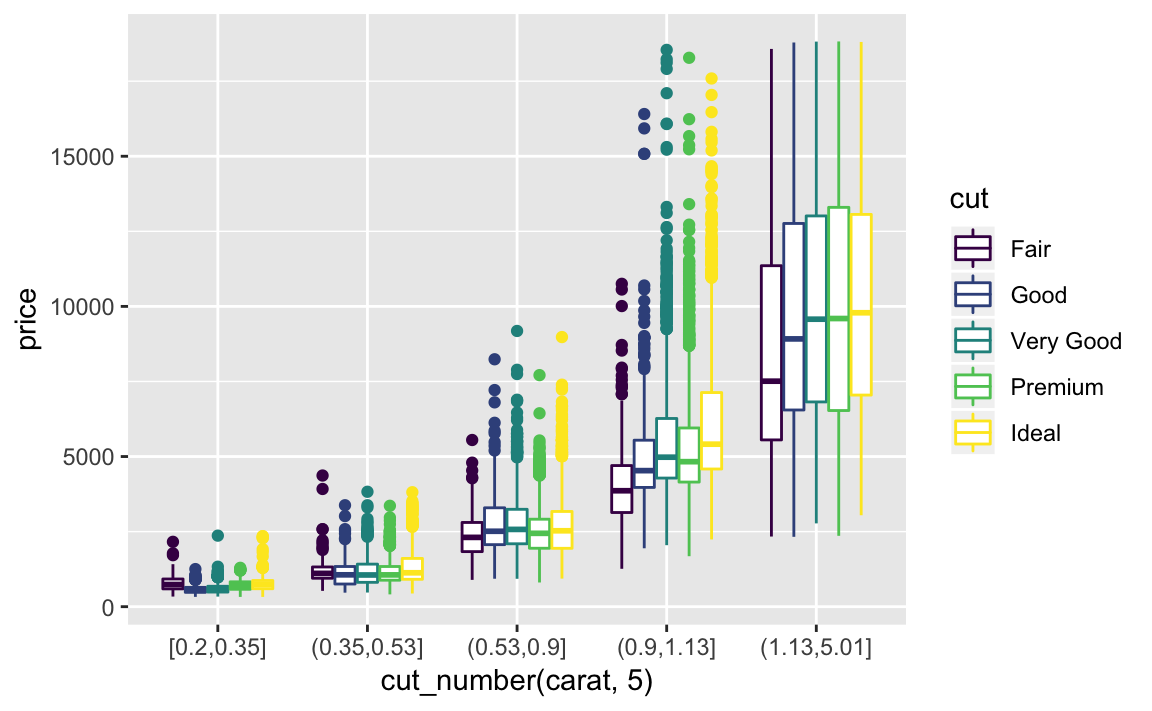
\includegraphics[width=0.7\linewidth]{visualize_files/figure-latex/unnamed-chunk-42-1} \end{center}

However, we can adjust them. Here are few examples to understand how
adjusting these parameters affects the look of the plot.

With \texttt{width\ =\ 0} there is no horizontal jitter.

\begin{Shaded}
\begin{Highlighting}[]
\KeywordTok{ggplot}\NormalTok{(}\DataTypeTok{data =}\NormalTok{ mpg, }\DataTypeTok{mapping =} \KeywordTok{aes}\NormalTok{(}\DataTypeTok{x =}\NormalTok{ cty, }\DataTypeTok{y =}\NormalTok{ hwy)) }\OperatorTok{+}
\StringTok{  }\KeywordTok{geom_jitter}\NormalTok{(}\DataTypeTok{width =} \DecValTok{0}\NormalTok{)}
\end{Highlighting}
\end{Shaded}

\begin{center}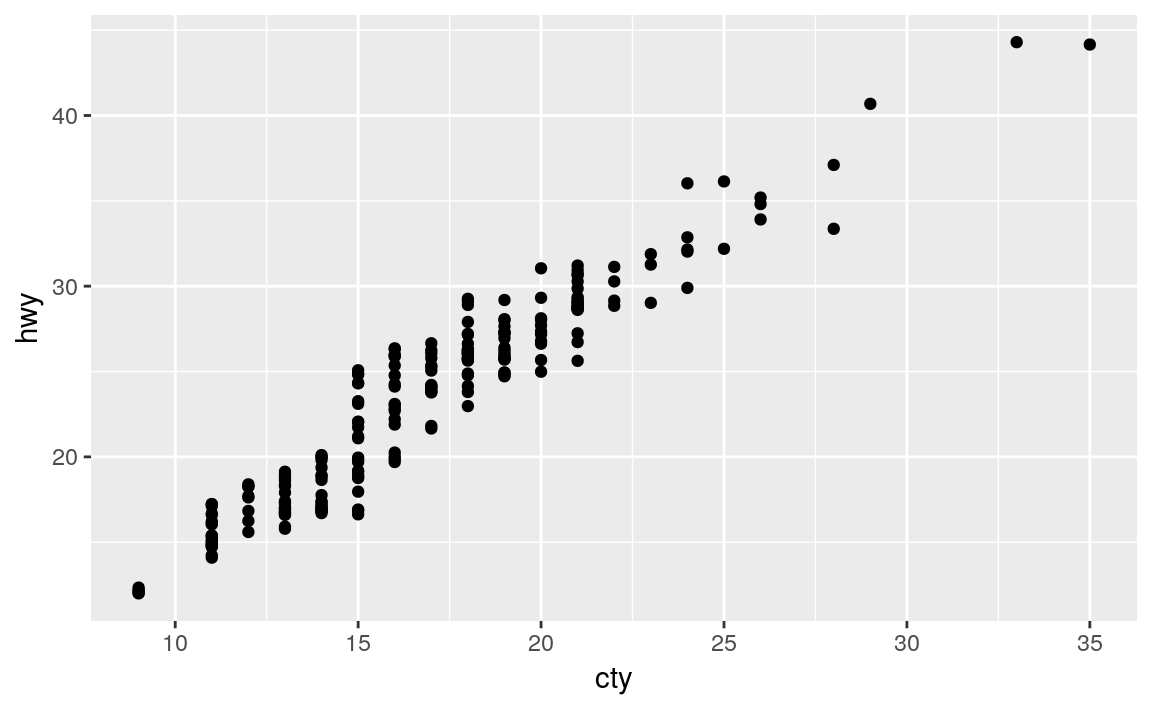
\includegraphics[width=0.7\linewidth]{visualize_files/figure-latex/unnamed-chunk-43-1} \end{center}

With \texttt{width\ =\ 20}, there is too much horizontal jitter.

\begin{Shaded}
\begin{Highlighting}[]
\KeywordTok{ggplot}\NormalTok{(}\DataTypeTok{data =}\NormalTok{ mpg, }\DataTypeTok{mapping =} \KeywordTok{aes}\NormalTok{(}\DataTypeTok{x =}\NormalTok{ cty, }\DataTypeTok{y =}\NormalTok{ hwy)) }\OperatorTok{+}
\StringTok{  }\KeywordTok{geom_jitter}\NormalTok{(}\DataTypeTok{width =} \DecValTok{20}\NormalTok{)}
\end{Highlighting}
\end{Shaded}

\begin{center}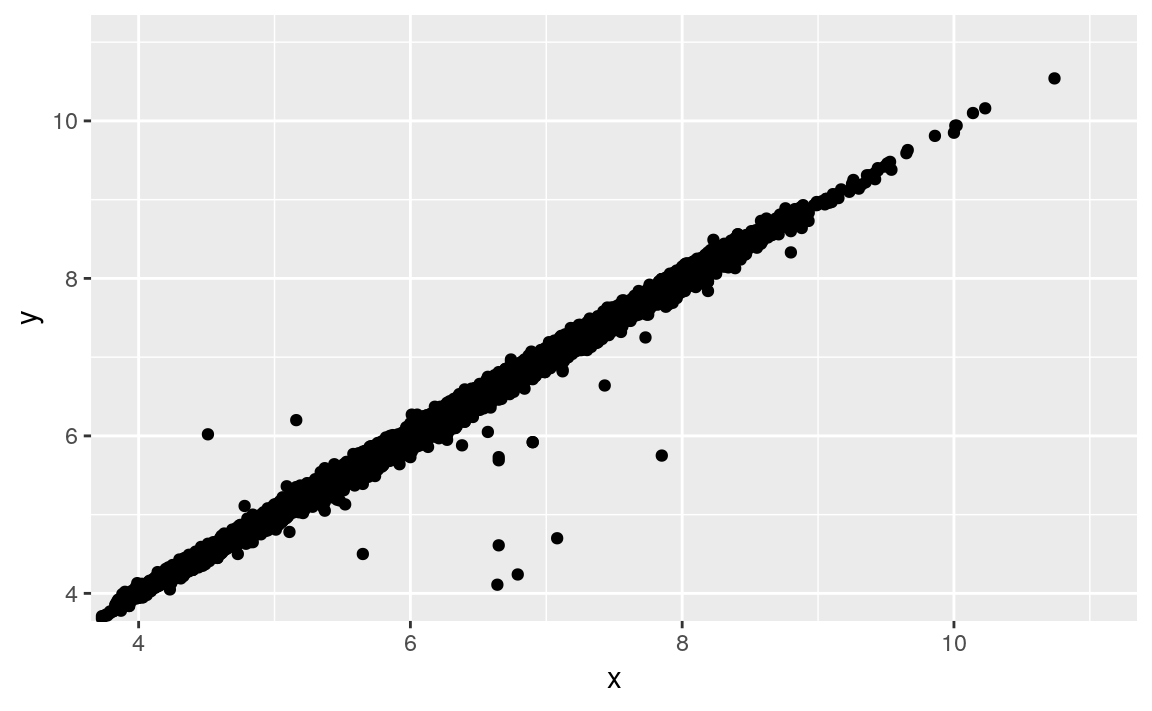
\includegraphics[width=0.7\linewidth]{visualize_files/figure-latex/unnamed-chunk-44-1} \end{center}

With \texttt{height\ =\ 0}, there is no vertical horizontal jitter:

\begin{Shaded}
\begin{Highlighting}[]
\KeywordTok{ggplot}\NormalTok{(}\DataTypeTok{data =}\NormalTok{ mpg, }\DataTypeTok{mapping =} \KeywordTok{aes}\NormalTok{(}\DataTypeTok{x =}\NormalTok{ cty, }\DataTypeTok{y =}\NormalTok{ hwy)) }\OperatorTok{+}
\StringTok{  }\KeywordTok{geom_jitter}\NormalTok{(}\DataTypeTok{height =} \DecValTok{0}\NormalTok{)}
\end{Highlighting}
\end{Shaded}

\begin{center}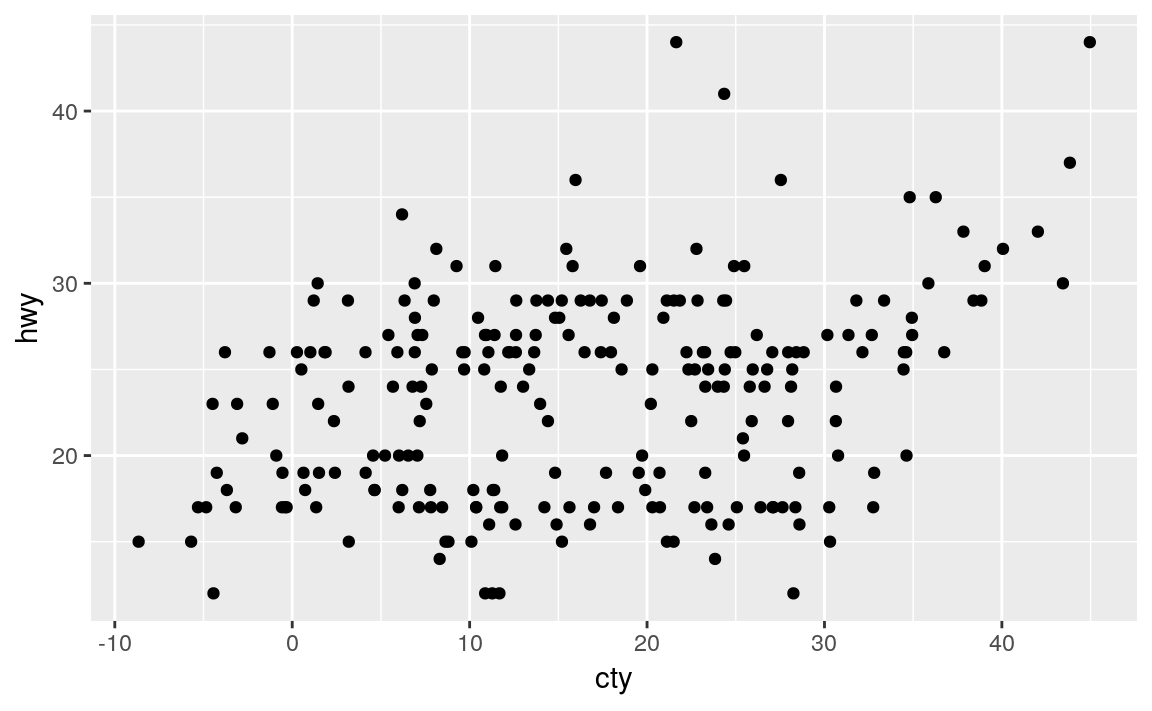
\includegraphics[width=0.7\linewidth]{visualize_files/figure-latex/unnamed-chunk-45-1} \end{center}

With \texttt{height\ =\ 15}, there is too much vertical jitter.

\begin{Shaded}
\begin{Highlighting}[]
\KeywordTok{ggplot}\NormalTok{(}\DataTypeTok{data =}\NormalTok{ mpg, }\DataTypeTok{mapping =} \KeywordTok{aes}\NormalTok{(}\DataTypeTok{x =}\NormalTok{ cty, }\DataTypeTok{y =}\NormalTok{ hwy)) }\OperatorTok{+}
\StringTok{  }\KeywordTok{geom_point}\NormalTok{(}\DataTypeTok{height =} \DecValTok{15}\NormalTok{)}
\CommentTok{#> Warning: Ignoring unknown parameters: height}
\end{Highlighting}
\end{Shaded}

\begin{center}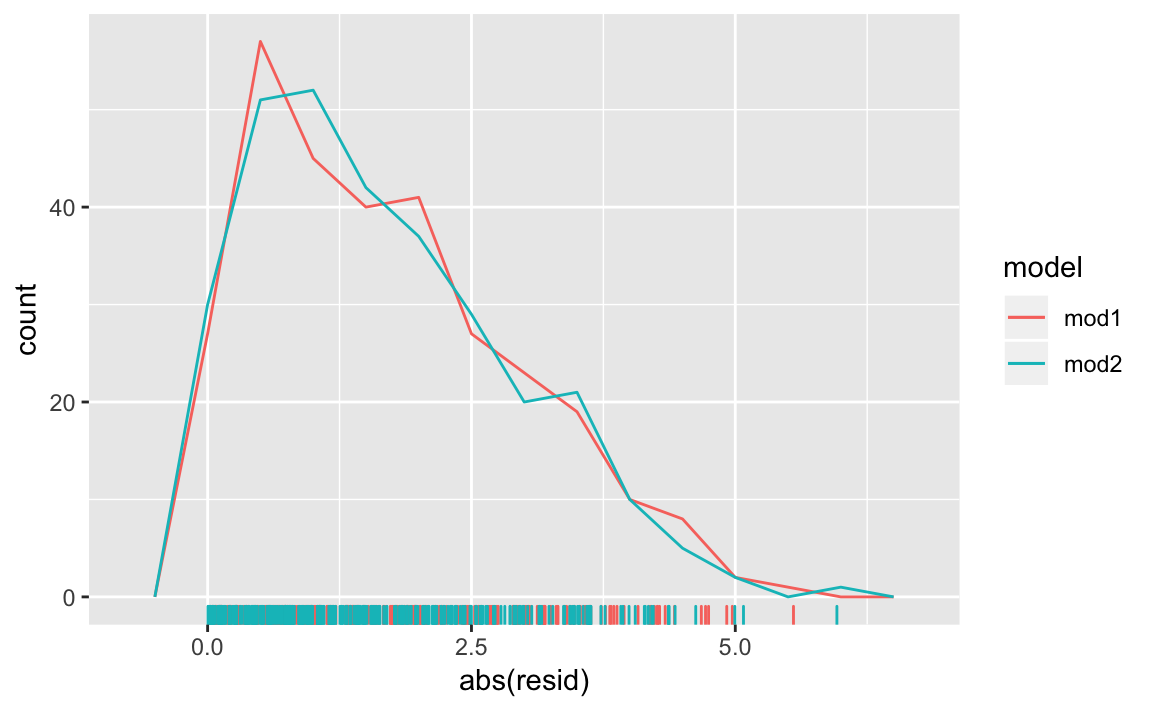
\includegraphics[width=0.7\linewidth]{visualize_files/figure-latex/unnamed-chunk-46-1} \end{center}

Note that the \texttt{height} and \texttt{width} arguments are in the
units of the data. Thus \texttt{height\ =\ 1} corresponds to different
relative amounts of jittering depending on the scale of the \texttt{y}
variable. The default values of \texttt{height} and \texttt{width} are
defined to be 80\% of the \texttt{resolution()} of the data, which is
the smallest non-zero distance between adjacent values of a variable.
This means that if \texttt{x} and \texttt{y} are discrete variables,
their resolutions are both equal to 1, and \texttt{height\ =\ 0.8} and
\texttt{width\ =\ 0.8}.

\hypertarget{exercise-3.8.1.3.}{%
\subsection*{\texorpdfstring{Exercise
{3.8.1.3}.}{Exercise 3.8.1.3.}}\label{exercise-3.8.1.3.}}
\addcontentsline{toc}{subsection}{Exercise {3.8.1.3}.}

Compare and contrast \texttt{geom\_jitter()} with
\texttt{geom\_count()}.

\texttt{geom\_jitter()} adds random noise to the locations points of the
graph. In other words, it ``jitters'' the points. This method reduces
overplotting since no two points are likely to have the same location
after the random noise is added to their locations.

\begin{Shaded}
\begin{Highlighting}[]
\KeywordTok{ggplot}\NormalTok{(}\DataTypeTok{data =}\NormalTok{ mpg, }\DataTypeTok{mapping =} \KeywordTok{aes}\NormalTok{(}\DataTypeTok{x =}\NormalTok{ cty, }\DataTypeTok{y =}\NormalTok{ hwy)) }\OperatorTok{+}
\StringTok{  }\KeywordTok{geom_jitter}\NormalTok{()}
\end{Highlighting}
\end{Shaded}

\begin{center}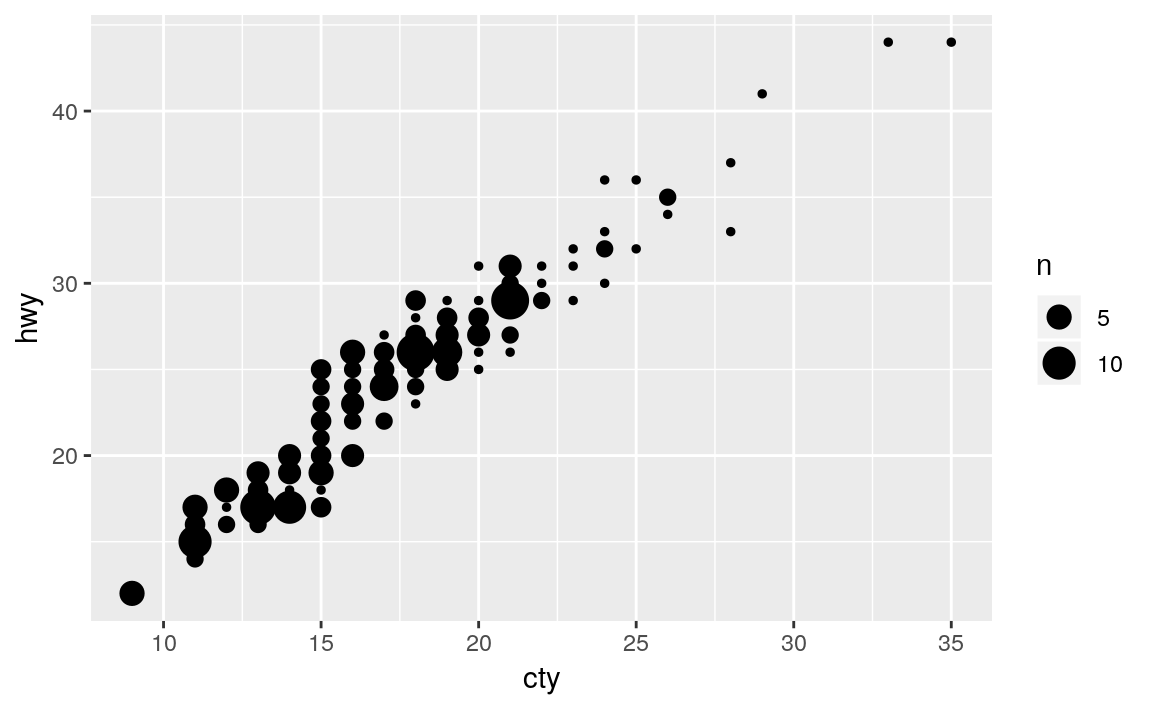
\includegraphics[width=0.7\linewidth]{visualize_files/figure-latex/unnamed-chunk-47-1} \end{center}

However, the reduction in overlapping comes at the cost of changing the
\texttt{x} and \texttt{y} values of the points.

\texttt{geom\_count()} resizes the points relative to the number of
observations at each location. In other words, points with more
observations will be larger than those with fewer observations.

\begin{Shaded}
\begin{Highlighting}[]
\KeywordTok{ggplot}\NormalTok{(}\DataTypeTok{data =}\NormalTok{ mpg, }\DataTypeTok{mapping =} \KeywordTok{aes}\NormalTok{(}\DataTypeTok{x =}\NormalTok{ cty, }\DataTypeTok{y =}\NormalTok{ hwy)) }\OperatorTok{+}
\StringTok{  }\KeywordTok{geom_count}\NormalTok{()}
\end{Highlighting}
\end{Shaded}

\begin{center}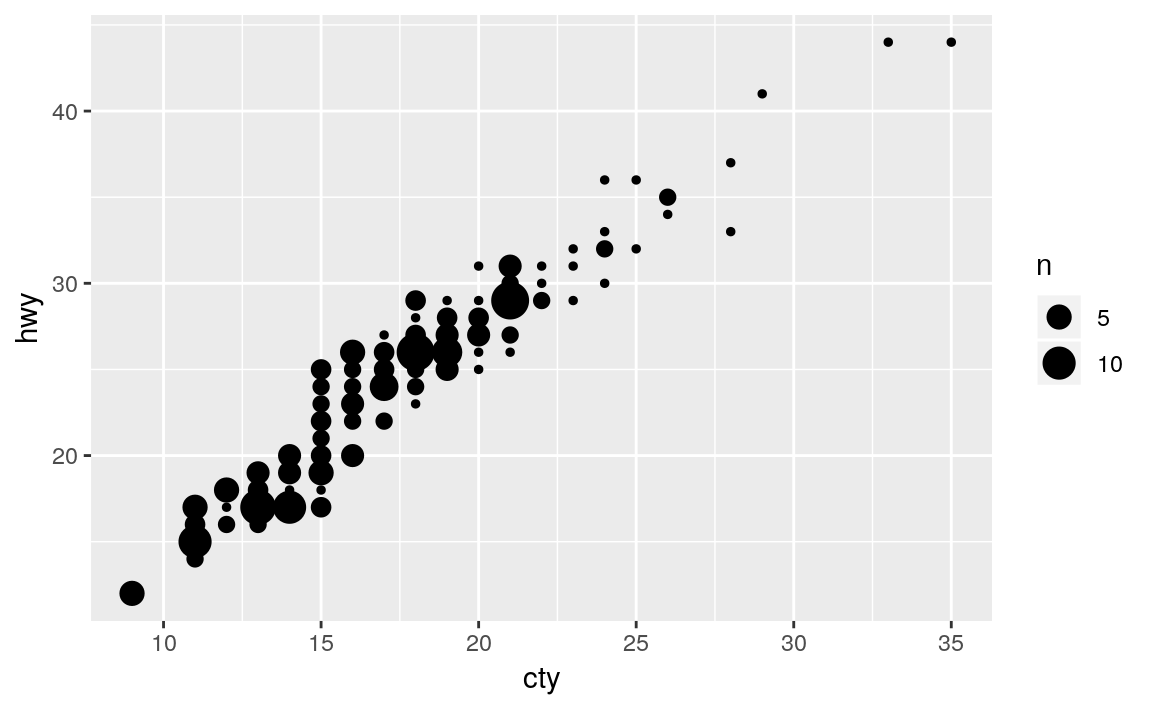
\includegraphics[width=0.7\linewidth]{visualize_files/figure-latex/unnamed-chunk-48-1} \end{center}

This method does not change the \texttt{x} and \texttt{y} coordinates of
the points. However, if the points are close together and counts are
large, the size of some points can itself introduce overplotting. For
example, in the following example a third variable mapped to color is
added to the plot. In this case, \texttt{geom\_count()} is less readable
than \texttt{geom\_jitter()} when adding a third variable as color
aesthetic.

\begin{Shaded}
\begin{Highlighting}[]
\KeywordTok{ggplot}\NormalTok{(}\DataTypeTok{data =}\NormalTok{ mpg, }\DataTypeTok{mapping =} \KeywordTok{aes}\NormalTok{(}\DataTypeTok{x =}\NormalTok{ cty, }\DataTypeTok{y =}\NormalTok{ hwy, }\DataTypeTok{color =}\NormalTok{ class)) }\OperatorTok{+}
\StringTok{  }\KeywordTok{geom_jitter}\NormalTok{()}
\end{Highlighting}
\end{Shaded}

\begin{center}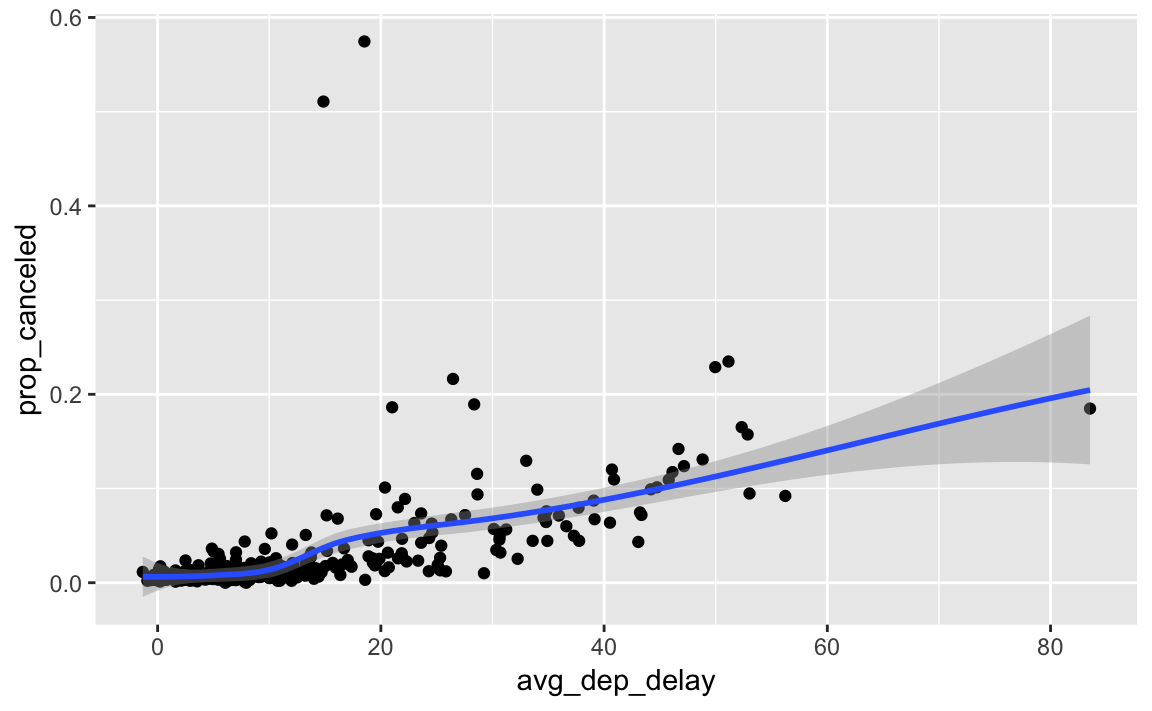
\includegraphics[width=0.7\linewidth]{visualize_files/figure-latex/unnamed-chunk-49-1} \end{center}

\begin{Shaded}
\begin{Highlighting}[]
\KeywordTok{ggplot}\NormalTok{(}\DataTypeTok{data =}\NormalTok{ mpg, }\DataTypeTok{mapping =} \KeywordTok{aes}\NormalTok{(}\DataTypeTok{x =}\NormalTok{ cty, }\DataTypeTok{y =}\NormalTok{ hwy, }\DataTypeTok{color =}\NormalTok{ class)) }\OperatorTok{+}
\StringTok{  }\KeywordTok{geom_count}\NormalTok{()}
\end{Highlighting}
\end{Shaded}

\begin{center}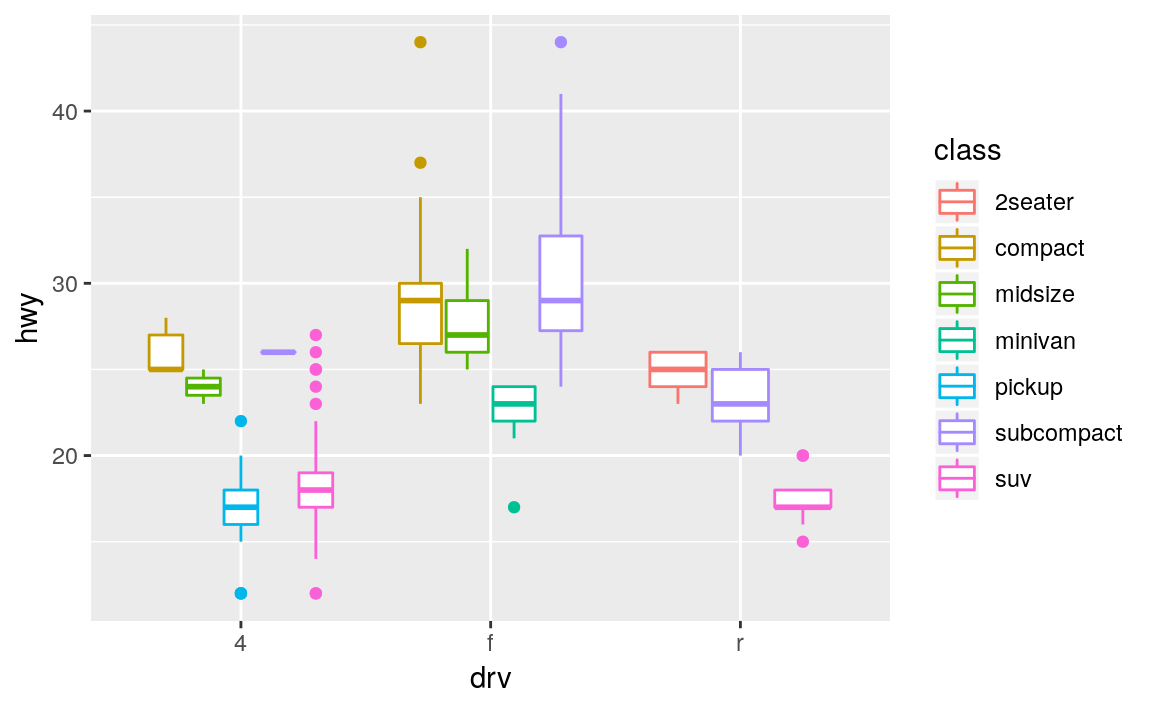
\includegraphics[width=0.7\linewidth]{visualize_files/figure-latex/unnamed-chunk-50-1} \end{center}

Unfortunately, there is no universal solution to overplotting. The costs
and benefits of different approaches will depend on the structure of the
data and the goal of the data scientist.

\hypertarget{exercise-3.8.1.4.}{%
\subsection*{\texorpdfstring{Exercise
{3.8.1.4}.}{Exercise 3.8.1.4.}}\label{exercise-3.8.1.4.}}
\addcontentsline{toc}{subsection}{Exercise {3.8.1.4}.}

What's the default position adjustment for \texttt{geom\_boxplot()}?
Create a visualization of the mpg dataset that demonstrates it.

The default position for \texttt{geom\_boxplot()} is
\texttt{position\_dodge()} (see its
\href{https://ggplot2.tidyverse.org/reference/geom_boxplot.html}{docs}).

When we add \texttt{colour\ =\ class} to the box plot, the different
classes within \texttt{drv} are placed side by side, i.e.~dodged. If it
was \texttt{position\_identity()}, they would be overlapping.

\begin{Shaded}
\begin{Highlighting}[]
\KeywordTok{ggplot}\NormalTok{(}\DataTypeTok{data =}\NormalTok{ mpg, }\KeywordTok{aes}\NormalTok{(}\DataTypeTok{x =}\NormalTok{ drv, }\DataTypeTok{y =}\NormalTok{ hwy, }\DataTypeTok{colour =}\NormalTok{ class)) }\OperatorTok{+}
\StringTok{  }\KeywordTok{geom_boxplot}\NormalTok{()}
\end{Highlighting}
\end{Shaded}

\begin{center}\includegraphics[width=0.7\linewidth]{visualize_files/figure-latex/unnamed-chunk-51-1} \end{center}

\begin{Shaded}
\begin{Highlighting}[]
\KeywordTok{ggplot}\NormalTok{(}\DataTypeTok{data =}\NormalTok{ mpg, }\KeywordTok{aes}\NormalTok{(}\DataTypeTok{x =}\NormalTok{ drv, }\DataTypeTok{y =}\NormalTok{ hwy, }\DataTypeTok{colour =}\NormalTok{ class)) }\OperatorTok{+}
\StringTok{  }\KeywordTok{geom_boxplot}\NormalTok{(}\DataTypeTok{position =} \StringTok{"identity"}\NormalTok{)}
\end{Highlighting}
\end{Shaded}

\begin{center}\includegraphics[width=0.7\linewidth]{visualize_files/figure-latex/unnamed-chunk-52-1} \end{center}

\hypertarget{coordinate-systems}{%
\section{Coordinate Systems}\label{coordinate-systems}}

\hypertarget{exercise-3.9.1.1}{%
\subsection*{\texorpdfstring{Exercise
{3.9.1.1}}{Exercise 3.9.1.1}}\label{exercise-3.9.1.1}}
\addcontentsline{toc}{subsection}{Exercise {3.9.1.1}}

Turn a stacked bar chart into a pie chart using \texttt{coord\_polar()}.

This is a stacked bar chart with a single category

\begin{Shaded}
\begin{Highlighting}[]
\KeywordTok{ggplot}\NormalTok{(mpg, }\KeywordTok{aes}\NormalTok{(}\DataTypeTok{x =} \KeywordTok{factor}\NormalTok{(}\DecValTok{1}\NormalTok{), }\DataTypeTok{fill =}\NormalTok{ drv)) }\OperatorTok{+}
\StringTok{  }\KeywordTok{geom_bar}\NormalTok{()}
\end{Highlighting}
\end{Shaded}

\begin{center}\includegraphics[width=0.7\linewidth]{visualize_files/figure-latex/unnamed-chunk-53-1} \end{center}

See the documentation for
\href{https://ggplot2.tidyverse.org/reference/coord_polar.html}{coord\_polar}
for an example of making a pie chart. In particular,
\texttt{theta\ =\ "y"}, meaning that the angle of the chart is the
\texttt{y} variable which has to be specified.

\begin{Shaded}
\begin{Highlighting}[]
\KeywordTok{ggplot}\NormalTok{(mpg, }\KeywordTok{aes}\NormalTok{(}\DataTypeTok{x =} \KeywordTok{factor}\NormalTok{(}\DecValTok{1}\NormalTok{), }\DataTypeTok{fill =}\NormalTok{ drv)) }\OperatorTok{+}
\StringTok{  }\KeywordTok{geom_bar}\NormalTok{(}\DataTypeTok{width =} \DecValTok{1}\NormalTok{) }\OperatorTok{+}
\StringTok{  }\KeywordTok{coord_polar}\NormalTok{(}\DataTypeTok{theta =} \StringTok{"y"}\NormalTok{)}
\end{Highlighting}
\end{Shaded}

\begin{center}\includegraphics[width=0.7\linewidth]{visualize_files/figure-latex/unnamed-chunk-54-1} \end{center}

If \texttt{theta\ =\ "y"} is not specified, then you get a bull's-eye
chart

\begin{Shaded}
\begin{Highlighting}[]
\KeywordTok{ggplot}\NormalTok{(mpg, }\KeywordTok{aes}\NormalTok{(}\DataTypeTok{x =} \KeywordTok{factor}\NormalTok{(}\DecValTok{1}\NormalTok{), }\DataTypeTok{fill =}\NormalTok{ drv)) }\OperatorTok{+}
\StringTok{  }\KeywordTok{geom_bar}\NormalTok{(}\DataTypeTok{width =} \DecValTok{1}\NormalTok{) }\OperatorTok{+}
\StringTok{  }\KeywordTok{coord_polar}\NormalTok{()}
\end{Highlighting}
\end{Shaded}

\begin{center}\includegraphics[width=0.7\linewidth]{visualize_files/figure-latex/unnamed-chunk-55-1} \end{center}

If you had a multiple stacked bar chart,

\begin{Shaded}
\begin{Highlighting}[]
\KeywordTok{ggplot}\NormalTok{(}\DataTypeTok{data =}\NormalTok{ diamonds) }\OperatorTok{+}
\StringTok{  }\KeywordTok{geom_bar}\NormalTok{(}\DataTypeTok{mapping =} \KeywordTok{aes}\NormalTok{(}\DataTypeTok{x =}\NormalTok{ cut, }\DataTypeTok{fill =}\NormalTok{ clarity), }\DataTypeTok{position =} \StringTok{"fill"}\NormalTok{)}
\end{Highlighting}
\end{Shaded}

\begin{center}\includegraphics[width=0.7\linewidth]{visualize_files/figure-latex/unnamed-chunk-56-1} \end{center}

and apply polar coordinates to it, you end up with a multi-doughnut
chart,

\begin{Shaded}
\begin{Highlighting}[]
\KeywordTok{ggplot}\NormalTok{(}\DataTypeTok{data =}\NormalTok{ diamonds) }\OperatorTok{+}
\StringTok{  }\KeywordTok{geom_bar}\NormalTok{(}\DataTypeTok{mapping =} \KeywordTok{aes}\NormalTok{(}\DataTypeTok{x =}\NormalTok{ cut, }\DataTypeTok{fill =}\NormalTok{ clarity), }\DataTypeTok{position =} \StringTok{"fill"}\NormalTok{) }\OperatorTok{+}
\StringTok{  }\KeywordTok{coord_polar}\NormalTok{(}\DataTypeTok{theta =} \StringTok{"y"}\NormalTok{)}
\end{Highlighting}
\end{Shaded}

\begin{center}\includegraphics[width=0.7\linewidth]{visualize_files/figure-latex/unnamed-chunk-57-1} \end{center}

\hypertarget{exercise-3.9.1.2}{%
\subsection*{\texorpdfstring{Exercise
{3.9.1.2}}{Exercise 3.9.1.2}}\label{exercise-3.9.1.2}}
\addcontentsline{toc}{subsection}{Exercise {3.9.1.2}}

What does \texttt{labs()} do? Read the documentation.

The \texttt{labs} function adds labels for different scales and the
title of the plot.

\begin{Shaded}
\begin{Highlighting}[]
\KeywordTok{ggplot}\NormalTok{(}\DataTypeTok{data =}\NormalTok{ mpg, }\DataTypeTok{mapping =} \KeywordTok{aes}\NormalTok{(}\DataTypeTok{x =}\NormalTok{ class, }\DataTypeTok{y =}\NormalTok{ hwy)) }\OperatorTok{+}
\StringTok{  }\KeywordTok{geom_boxplot}\NormalTok{() }\OperatorTok{+}
\StringTok{  }\KeywordTok{coord_flip}\NormalTok{() }\OperatorTok{+}
\StringTok{  }\KeywordTok{labs}\NormalTok{(}\DataTypeTok{y =} \StringTok{"Highway MPG"}\NormalTok{, }\DataTypeTok{x =} \StringTok{""}\NormalTok{, }\DataTypeTok{title =} \StringTok{"Highway MPG by car class"}\NormalTok{)}
\end{Highlighting}
\end{Shaded}

\begin{center}\includegraphics[width=0.7\linewidth]{visualize_files/figure-latex/unnamed-chunk-58-1} \end{center}

\hypertarget{exercise-3.9.1.3}{%
\subsection*{\texorpdfstring{Exercise
{3.9.1.3}}{Exercise 3.9.1.3}}\label{exercise-3.9.1.3}}
\addcontentsline{toc}{subsection}{Exercise {3.9.1.3}}

What's the difference between \texttt{coord\_quickmap()} and
\texttt{coord\_map()}?

\texttt{coord\_map()} uses map projection to project 3-dimensional Earth
onto a 2-dimensional plane. By default, \texttt{coord\_map()} uses the
\href{https://en.wikipedia.org/wiki/Mercator_projection}{Mercator
projection}. However, this projection must be applied to all geoms in
the plot. \texttt{coord\_quickmap()} uses a faster, but approximate map
projection. This approximation ignores the curvature of Earth and
adjusts the map for the latitude/longitude ratio. This transformation is
quicker than \texttt{coord\_map()} because the coordinates of the
individual geoms do not need to be transformed.

The \textbf{ggplot2}
\href{https://ggplot2.tidyverse.org/reference/coord_map.html}{documentation}
contains more information on and examples for these two functions.

\hypertarget{exercise-3.9.1.4}{%
\subsection*{\texorpdfstring{Exercise
{3.9.1.4}}{Exercise 3.9.1.4}}\label{exercise-3.9.1.4}}
\addcontentsline{toc}{subsection}{Exercise {3.9.1.4}}

What does the plot below tell you about the relationship between city
and highway mpg? Why is \texttt{coord\_fixed()} important? What does
\texttt{geom\_abline()} do?

The function \texttt{coord\_fixed()} ensures that the line produced by
\texttt{geom\_abline()} is at a 45 degree angle. The 45 degree line
makes it easy to compare the highway and city mileage to the case in
which city and highway MPG were equal.

\begin{Shaded}
\begin{Highlighting}[]
\NormalTok{p <-}\StringTok{ }\KeywordTok{ggplot}\NormalTok{(}\DataTypeTok{data =}\NormalTok{ mpg, }\DataTypeTok{mapping =} \KeywordTok{aes}\NormalTok{(}\DataTypeTok{x =}\NormalTok{ cty, }\DataTypeTok{y =}\NormalTok{ hwy)) }\OperatorTok{+}
\StringTok{  }\KeywordTok{geom_point}\NormalTok{() }\OperatorTok{+}
\StringTok{  }\KeywordTok{geom_abline}\NormalTok{()}
\NormalTok{p }\OperatorTok{+}\StringTok{ }\KeywordTok{coord_fixed}\NormalTok{()}
\end{Highlighting}
\end{Shaded}

\begin{center}\includegraphics[width=0.7\linewidth]{visualize_files/figure-latex/unnamed-chunk-59-1} \end{center}

If we didn't include \texttt{geom\_coord()}, then the line would no
longer have an angle of 45 degrees.

\begin{Shaded}
\begin{Highlighting}[]
\NormalTok{p}
\end{Highlighting}
\end{Shaded}

\begin{center}\includegraphics[width=0.7\linewidth]{visualize_files/figure-latex/unnamed-chunk-60-1} \end{center}

On average, humans are best able to perceive differences in angles
relative to 45 degrees. See Cleveland
(\protect\hyperlink{ref-Cleveland1993}{1993}\protect\hyperlink{ref-Cleveland1993}{b}),
Cleveland (\protect\hyperlink{ref-Cleveland1994}{1994}),Cleveland
(\protect\hyperlink{ref-Cleveland1993a}{1993}\protect\hyperlink{ref-Cleveland1993a}{a}),
Cleveland, McGill, and McGill
(\protect\hyperlink{ref-ClevelandMcGillMcGill1988}{1988}), Heer and
Agrawala (\protect\hyperlink{ref-HeerAgrawala2006}{2006}) for discussion
on how the aspect ratio of a plot affects perception of the values it
encodes, evidence that 45 degrees is generally optimal, and methods to
calculate the an aspect ratio to achieve it. The function
\texttt{ggthemes::bank\_slopes()} will calculate the optimal aspect
ratio to bank slopes to 45 degrees.

\hypertarget{the-layered-grammar-of-graphics}{%
\section{The Layered Grammar of
Graphics}\label{the-layered-grammar-of-graphics}}

No exercises

\hypertarget{workflow-basics}{%
\chapter{Workflow: basics}\label{workflow-basics}}

\hypertarget{prerequisites}{%
\section*{Prerequisites}\label{prerequisites}}
\addcontentsline{toc}{section}{Prerequisites}

\begin{Shaded}
\begin{Highlighting}[]
\KeywordTok{library}\NormalTok{(}\StringTok{"tidyverse"}\NormalTok{)}
\end{Highlighting}
\end{Shaded}

\hypertarget{coding-basics}{%
\section{Coding basics}\label{coding-basics}}

No exercises

\hypertarget{whats-in-a-name}{%
\section{What's in a name?}\label{whats-in-a-name}}

No exercises

\hypertarget{calling-functions}{%
\section{Calling functions}\label{calling-functions}}

No exercises

\hypertarget{practice}{%
\section{Practice}\label{practice}}

\hypertarget{exercise-4.4.1}{%
\subsection*{\texorpdfstring{Exercise
{4.4.1}}{Exercise 4.4.1}}\label{exercise-4.4.1}}
\addcontentsline{toc}{subsection}{Exercise {4.4.1}}

Why does this code not work?

\begin{Shaded}
\begin{Highlighting}[]
\NormalTok{my_variable <-}\StringTok{ }\DecValTok{10}
\NormalTok{my_varıable}
\CommentTok{#> Error in eval(expr, envir, enclos): object 'my_varıable' not found}
\end{Highlighting}
\end{Shaded}

The variable being printed is \texttt{my\_varıable}, not
\texttt{my\_variable}: the seventh character is ``ı''
(``\href{https://en.wikipedia.org/wiki/Dotted_and_dotless_I}{LATIN SMALL
LETTER DOTLESS I}''), not ``i''.

While it wouldn't have helped much in this case, the importance of
distinguishing characters in code is reasons why fonts which clearly
distinguish similar characters are preferred in programming. It is
especially important to distinguish between two sets of similar looking
characters:

\begin{itemize}
\tightlist
\item
  the numeral zero (0), the Latin small letter O (o), and the Latin
  capital letter O (O),
\item
  the numeral one (1), the Latin small letter I (i), the Latin capital
  letter I (I), and Latin small letter L (l).
\end{itemize}

In these fonts, zero and the Latin letter O are often distinguished by
using a glyph for zero that uses either a dot in the interior or a slash
through it. Some examples of fonts with dotted or slashed zero glyphs
are Consolas, Deja Vu Sans Mono, Monaco, Menlo,
\href{https://adobe-fonts.github.io/source-sans-pro/}{Source Sans Pro},
and FiraCode.

Error messages of the form
\texttt{"object\ \textquotesingle{}...\textquotesingle{}\ not\ found"}
mean exactly what they say. R cannot find an object with that name.
Unfortunately, the error does not tell you why that object cannot be
found, because R does not know the reason that the object does not
exist. The most common scenarios in which I encounter this error message
are

\begin{enumerate}
\def\labelenumi{\arabic{enumi}.}
\item
  I forgot to create the object, or an error prevented the object from
  being created.
\item
  I made a typo in the object's name, either when using it or when I
  created it (as in the example above), or I forgot what I had
  originally named it. If you find yourself often writing the wrong name
  for an object, it is a good indication that the original name was not
  a good one.
\item
  I forgot to load the package that contains the object using
  \texttt{library()}.
\end{enumerate}

\hypertarget{exercise-4.4.2}{%
\subsection*{\texorpdfstring{Exercise
{4.4.2}}{Exercise 4.4.2}}\label{exercise-4.4.2}}
\addcontentsline{toc}{subsection}{Exercise {4.4.2}}

Tweak each of the following R commands so that they run correctly:

\begin{Shaded}
\begin{Highlighting}[]
\KeywordTok{ggplot}\NormalTok{(}\DataTypeTok{dota =}\NormalTok{ mpg) }\OperatorTok{+}
\StringTok{  }\KeywordTok{geom_point}\NormalTok{(}\DataTypeTok{mapping =} \KeywordTok{aes}\NormalTok{(}\DataTypeTok{x =}\NormalTok{ displ, }\DataTypeTok{y =}\NormalTok{ hwy))}
\CommentTok{#> Error in FUN(X[[i]], ...): object 'displ' not found}
\end{Highlighting}
\end{Shaded}

\begin{center}\includegraphics[width=0.7\linewidth]{workflow-basics_files/figure-latex/unnamed-chunk-4-1} \end{center}

The error message is
\texttt{argument\ "data"\ is\ missing,\ with\ no\ default}.

It looks like a typo, \texttt{dota} instead of \texttt{data}.

\begin{Shaded}
\begin{Highlighting}[]
\KeywordTok{ggplot}\NormalTok{(}\DataTypeTok{data =}\NormalTok{ mpg) }\OperatorTok{+}
\StringTok{  }\KeywordTok{geom_point}\NormalTok{(}\DataTypeTok{mapping =} \KeywordTok{aes}\NormalTok{(}\DataTypeTok{x =}\NormalTok{ displ, }\DataTypeTok{y =}\NormalTok{ hwy))}
\end{Highlighting}
\end{Shaded}

\begin{center}\includegraphics[width=0.7\linewidth]{workflow-basics_files/figure-latex/unnamed-chunk-5-1} \end{center}

\begin{Shaded}
\begin{Highlighting}[]
\KeywordTok{fliter}\NormalTok{(mpg, }\DataTypeTok{cyl =} \DecValTok{8}\NormalTok{)}
\CommentTok{#> Error in fliter(mpg, cyl = 8): could not find function "fliter"}
\end{Highlighting}
\end{Shaded}

R could not find the function \texttt{fliter()} because we made a typo:
\texttt{fliter} instead of \texttt{filter}.

\begin{Shaded}
\begin{Highlighting}[]
\KeywordTok{filter}\NormalTok{(mpg, }\DataTypeTok{cyl =} \DecValTok{8}\NormalTok{)}
\CommentTok{#> Error: `cyl` (`cyl = 8`) must not be named, do you need `==`?}
\end{Highlighting}
\end{Shaded}

We aren't done yet. But the error message gives a suggestion. Let's
follow it.

\begin{Shaded}
\begin{Highlighting}[]
\KeywordTok{filter}\NormalTok{(mpg, cyl }\OperatorTok{==}\StringTok{ }\DecValTok{8}\NormalTok{)}
\CommentTok{#> # A tibble: 70 x 11}
\CommentTok{#>   manufacturer model displ  year   cyl trans drv     cty   hwy fl    class}
\CommentTok{#>   <chr>        <chr> <dbl> <int> <int> <chr> <chr> <int> <int> <chr> <chr>}
\CommentTok{#> 1 audi         a6 q~   4.2  2008     8 auto~ 4        16    23 p     mids~}
\CommentTok{#> 2 chevrolet    c150~   5.3  2008     8 auto~ r        14    20 r     suv  }
\CommentTok{#> 3 chevrolet    c150~   5.3  2008     8 auto~ r        11    15 e     suv  }
\CommentTok{#> 4 chevrolet    c150~   5.3  2008     8 auto~ r        14    20 r     suv  }
\CommentTok{#> 5 chevrolet    c150~   5.7  1999     8 auto~ r        13    17 r     suv  }
\CommentTok{#> 6 chevrolet    c150~   6    2008     8 auto~ r        12    17 r     suv  }
\CommentTok{#> # ... with 64 more rows}
\end{Highlighting}
\end{Shaded}

\begin{Shaded}
\begin{Highlighting}[]
\KeywordTok{filter}\NormalTok{(diamond, carat }\OperatorTok{>}\StringTok{ }\DecValTok{3}\NormalTok{)}
\CommentTok{#> Error in filter(diamond, carat > 3): object 'diamond' not found}
\end{Highlighting}
\end{Shaded}

R says it can't find the object \texttt{diamond}. This is a typo; the
data frame is named \texttt{diamonds}.

\begin{Shaded}
\begin{Highlighting}[]
\KeywordTok{filter}\NormalTok{(diamonds, carat }\OperatorTok{>}\StringTok{ }\DecValTok{3}\NormalTok{)}
\CommentTok{#> # A tibble: 32 x 10}
\CommentTok{#>   carat cut     color clarity depth table price     x     y     z}
\CommentTok{#>   <dbl> <ord>   <ord> <ord>   <dbl> <dbl> <int> <dbl> <dbl> <dbl>}
\CommentTok{#> 1  3.01 Premium I     I1       62.7    58  8040  9.1   8.97  5.67}
\CommentTok{#> 2  3.11 Fair    J     I1       65.9    57  9823  9.15  9.02  5.98}
\CommentTok{#> 3  3.01 Premium F     I1       62.2    56  9925  9.24  9.13  5.73}
\CommentTok{#> 4  3.05 Premium E     I1       60.9    58 10453  9.26  9.25  5.66}
\CommentTok{#> 5  3.02 Fair    I     I1       65.2    56 10577  9.11  9.02  5.91}
\CommentTok{#> 6  3.01 Fair    H     I1       56.1    62 10761  9.54  9.38  5.31}
\CommentTok{#> # ... with 26 more rows}
\end{Highlighting}
\end{Shaded}

How did I know? I started typing in \texttt{diamond} and RStudio
completed it to \texttt{diamonds}. Since \texttt{diamonds} includes the
variable \texttt{carat} and the code works, that appears to have been
the problem.

\hypertarget{exercise-4.4.3}{%
\subsection*{\texorpdfstring{Exercise
{4.4.3}}{Exercise 4.4.3}}\label{exercise-4.4.3}}
\addcontentsline{toc}{subsection}{Exercise {4.4.3}}

Press \emph{Alt + Shift + K}. What happens? How can you get to the same
place using the menus?

This gives a menu with keyboard shortcuts. This can be found in the menu
under \texttt{Tools\ -\textgreater{}\ Keyboard\ Shortcuts\ Help}.

\hypertarget{data-transformation}{%
\chapter{Data transformation}\label{data-transformation}}

\hypertarget{introduction-2}{%
\section{Introduction}\label{introduction-2}}

\begin{Shaded}
\begin{Highlighting}[]
\KeywordTok{library}\NormalTok{(}\StringTok{"nycflights13"}\NormalTok{)}
\KeywordTok{library}\NormalTok{(}\StringTok{"tidyverse"}\NormalTok{)}
\end{Highlighting}
\end{Shaded}

\hypertarget{filter-rows-with-filter}{%
\section{\texorpdfstring{Filter rows with
\texttt{filter()}}{Filter rows with filter()}}\label{filter-rows-with-filter}}

\hypertarget{exercise-5.2.4.1}{%
\subsection*{\texorpdfstring{Exercise
{5.2.4.1}}{Exercise 5.2.4.1}}\label{exercise-5.2.4.1}}
\addcontentsline{toc}{subsection}{Exercise {5.2.4.1}}

Find all flights that

\begin{enumerate}
\def\labelenumi{\arabic{enumi}.}
\tightlist
\item
  Had an arrival delay of two or more hours
\item
  Flew to Houston (IAH or HOU)
\item
  Were operated by United, American, or Delta
\item
  Departed in summer (July, August, and September)
\item
  Arrived more than two hours late, but didn't leave late
\item
  Were delayed by at least an hour, but made up over 30 minutes in
  flight
\item
  Departed between midnight and 6am (inclusive)
\end{enumerate}

The answer to each part follows.

\begin{enumerate}
\def\labelenumi{\arabic{enumi}.}
\item
  Since delay is in minutes, find flights whose arrival was delayed 120
  or more minutes.

\begin{Shaded}
\begin{Highlighting}[]
\KeywordTok{filter}\NormalTok{(flights, arr_delay }\OperatorTok{>=}\StringTok{ }\DecValTok{120}\NormalTok{)}
\CommentTok{#> # A tibble: 10,200 x 19}
\CommentTok{#>    year month   day dep_time sched_dep_time dep_delay arr_time}
\CommentTok{#>   <int> <int> <int>    <int>          <int>     <dbl>    <int>}
\CommentTok{#> 1  2013     1     1      811            630       101     1047}
\CommentTok{#> 2  2013     1     1      848           1835       853     1001}
\CommentTok{#> 3  2013     1     1      957            733       144     1056}
\CommentTok{#> 4  2013     1     1     1114            900       134     1447}
\CommentTok{#> 5  2013     1     1     1505           1310       115     1638}
\CommentTok{#> 6  2013     1     1     1525           1340       105     1831}
\CommentTok{#> # ... with 1.019e+04 more rows, and 12 more variables:}
\CommentTok{#> #   sched_arr_time <int>, arr_delay <dbl>, carrier <chr>, flight <int>,}
\CommentTok{#> #   tailnum <chr>, origin <chr>, dest <chr>, air_time <dbl>,}
\CommentTok{#> #   distance <dbl>, hour <dbl>, minute <dbl>, time_hour <dttm>}
\end{Highlighting}
\end{Shaded}
\item
  The flights that flew to Houston were are those flights where the
  destination (\texttt{dest}) is either ``IAH'' or ``HOU''.

\begin{Shaded}
\begin{Highlighting}[]
\KeywordTok{filter}\NormalTok{(flights, dest }\OperatorTok{==}\StringTok{ "IAH"} \OperatorTok{|}\StringTok{ }\NormalTok{dest }\OperatorTok{==}\StringTok{ "HOU"}\NormalTok{)}
\CommentTok{#> # A tibble: 9,313 x 19}
\CommentTok{#>    year month   day dep_time sched_dep_time dep_delay arr_time}
\CommentTok{#>   <int> <int> <int>    <int>          <int>     <dbl>    <int>}
\CommentTok{#> 1  2013     1     1      517            515         2      830}
\CommentTok{#> 2  2013     1     1      533            529         4      850}
\CommentTok{#> 3  2013     1     1      623            627        -4      933}
\CommentTok{#> 4  2013     1     1      728            732        -4     1041}
\CommentTok{#> 5  2013     1     1      739            739         0     1104}
\CommentTok{#> 6  2013     1     1      908            908         0     1228}
\CommentTok{#> # ... with 9,307 more rows, and 12 more variables: sched_arr_time <int>,}
\CommentTok{#> #   arr_delay <dbl>, carrier <chr>, flight <int>, tailnum <chr>,}
\CommentTok{#> #   origin <chr>, dest <chr>, air_time <dbl>, distance <dbl>, hour <dbl>,}
\CommentTok{#> #   minute <dbl>, time_hour <dttm>}
\end{Highlighting}
\end{Shaded}

  However, using \texttt{\%in\%} is more compact and would scale to
  cases where there were more than two airports we were interested in.

\begin{Shaded}
\begin{Highlighting}[]
\KeywordTok{filter}\NormalTok{(flights, dest }\OperatorTok\StringTok{ }\KeywordTok{c}\NormalTok{(}\StringTok{"IAH"}\NormalTok{, }\StringTok{"HOU"}\NormalTok{))}
\CommentTok{#> # A tibble: 9,313 x 19}
\CommentTok{#>    year month   day dep_time sched_dep_time dep_delay arr_time}
\CommentTok{#>   <int> <int> <int>    <int>          <int>     <dbl>    <int>}
\CommentTok{#> 1  2013     1     1      517            515         2      830}
\CommentTok{#> 2  2013     1     1      533            529         4      850}
\CommentTok{#> 3  2013     1     1      623            627        -4      933}
\CommentTok{#> 4  2013     1     1      728            732        -4     1041}
\CommentTok{#> 5  2013     1     1      739            739         0     1104}
\CommentTok{#> 6  2013     1     1      908            908         0     1228}
\CommentTok{#> # ... with 9,307 more rows, and 12 more variables: sched_arr_time <int>,}
\CommentTok{#> #   arr_delay <dbl>, carrier <chr>, flight <int>, tailnum <chr>,}
\CommentTok{#> #   origin <chr>, dest <chr>, air_time <dbl>, distance <dbl>, hour <dbl>,}
\CommentTok{#> #   minute <dbl>, time_hour <dttm>}
\end{Highlighting}
\end{Shaded}
\item
  In the \texttt{flights} dataset, the column \texttt{carrier} indicates
  the airline, but it uses two-character carrier codes. We can find the
  carrier codes for the airlines in the \texttt{airlines} dataset. Since
  the carrier code dataset only has 16 rows, and the names of the
  airlines in that dataset are not exactly ``United'', ``American'', or
  ``Delta'', it is easiest to manually look up their carrier codes in
  that data.

\begin{Shaded}
\begin{Highlighting}[]
\NormalTok{airlines}
\CommentTok{#> # A tibble: 16 x 2}
\CommentTok{#>   carrier name                    }
\CommentTok{#>   <chr>   <chr>                   }
\CommentTok{#> 1 9E      Endeavor Air Inc.       }
\CommentTok{#> 2 AA      American Airlines Inc.  }
\CommentTok{#> 3 AS      Alaska Airlines Inc.    }
\CommentTok{#> 4 B6      JetBlue Airways         }
\CommentTok{#> 5 DL      Delta Air Lines Inc.    }
\CommentTok{#> 6 EV      ExpressJet Airlines Inc.}
\CommentTok{#> # ... with 10 more rows}
\end{Highlighting}
\end{Shaded}

  The carrier code for Delta is \texttt{"DL"}, for American is
  \texttt{"AA"}, and for United is \texttt{"UA"}. Using these carriers
  codes, we check whether \texttt{carrier} is one of those.

\begin{Shaded}
\begin{Highlighting}[]
\KeywordTok{filter}\NormalTok{(flights, carrier }\OperatorTok\StringTok{ }\KeywordTok{c}\NormalTok{(}\StringTok{"AA"}\NormalTok{, }\StringTok{"DL"}\NormalTok{, }\StringTok{"UA"}\NormalTok{))}
\CommentTok{#> # A tibble: 139,504 x 19}
\CommentTok{#>    year month   day dep_time sched_dep_time dep_delay arr_time}
\CommentTok{#>   <int> <int> <int>    <int>          <int>     <dbl>    <int>}
\CommentTok{#> 1  2013     1     1      517            515         2      830}
\CommentTok{#> 2  2013     1     1      533            529         4      850}
\CommentTok{#> 3  2013     1     1      542            540         2      923}
\CommentTok{#> 4  2013     1     1      554            600        -6      812}
\CommentTok{#> 5  2013     1     1      554            558        -4      740}
\CommentTok{#> 6  2013     1     1      558            600        -2      753}
\CommentTok{#> # ... with 1.395e+05 more rows, and 12 more variables:}
\CommentTok{#> #   sched_arr_time <int>, arr_delay <dbl>, carrier <chr>, flight <int>,}
\CommentTok{#> #   tailnum <chr>, origin <chr>, dest <chr>, air_time <dbl>,}
\CommentTok{#> #   distance <dbl>, hour <dbl>, minute <dbl>, time_hour <dttm>}
\end{Highlighting}
\end{Shaded}
\item
  The variable \texttt{month} has the month, and it is numeric. So, the
  summer flights are those that departed in months 7 (July), 8 (August),
  and 9 (September).

\begin{Shaded}
\begin{Highlighting}[]
\KeywordTok{filter}\NormalTok{(flights, month }\OperatorTok{>=}\StringTok{ }\DecValTok{7}\NormalTok{, month }\OperatorTok{<=}\StringTok{ }\DecValTok{9}\NormalTok{)}
\CommentTok{#> # A tibble: 86,326 x 19}
\CommentTok{#>    year month   day dep_time sched_dep_time dep_delay arr_time}
\CommentTok{#>   <int> <int> <int>    <int>          <int>     <dbl>    <int>}
\CommentTok{#> 1  2013     7     1        1           2029       212      236}
\CommentTok{#> 2  2013     7     1        2           2359         3      344}
\CommentTok{#> 3  2013     7     1       29           2245       104      151}
\CommentTok{#> 4  2013     7     1       43           2130       193      322}
\CommentTok{#> 5  2013     7     1       44           2150       174      300}
\CommentTok{#> 6  2013     7     1       46           2051       235      304}
\CommentTok{#> # ... with 8.632e+04 more rows, and 12 more variables:}
\CommentTok{#> #   sched_arr_time <int>, arr_delay <dbl>, carrier <chr>, flight <int>,}
\CommentTok{#> #   tailnum <chr>, origin <chr>, dest <chr>, air_time <dbl>,}
\CommentTok{#> #   distance <dbl>, hour <dbl>, minute <dbl>, time_hour <dttm>}
\end{Highlighting}
\end{Shaded}

  The \texttt{\%in\%} and \texttt{\textbar{}} operators would also work,
  but using relational operators like \texttt{\textgreater{}=} and
  \texttt{\textless{}=} is preferred for numeric data.

\begin{Shaded}
\begin{Highlighting}[]
\KeywordTok{filter}\NormalTok{(flights, month }\OperatorTok\StringTok{  }\KeywordTok{c}\NormalTok{(}\DecValTok{7}\NormalTok{, }\DecValTok{8}\NormalTok{, }\DecValTok{9}\NormalTok{))}
\CommentTok{#> # A tibble: 86,326 x 19}
\CommentTok{#>    year month   day dep_time sched_dep_time dep_delay arr_time}
\CommentTok{#>   <int> <int> <int>    <int>          <int>     <dbl>    <int>}
\CommentTok{#> 1  2013     7     1        1           2029       212      236}
\CommentTok{#> 2  2013     7     1        2           2359         3      344}
\CommentTok{#> 3  2013     7     1       29           2245       104      151}
\CommentTok{#> 4  2013     7     1       43           2130       193      322}
\CommentTok{#> 5  2013     7     1       44           2150       174      300}
\CommentTok{#> 6  2013     7     1       46           2051       235      304}
\CommentTok{#> # ... with 8.632e+04 more rows, and 12 more variables:}
\CommentTok{#> #   sched_arr_time <int>, arr_delay <dbl>, carrier <chr>, flight <int>,}
\CommentTok{#> #   tailnum <chr>, origin <chr>, dest <chr>, air_time <dbl>,}
\CommentTok{#> #   distance <dbl>, hour <dbl>, minute <dbl>, time_hour <dttm>}
\end{Highlighting}
\end{Shaded}
\item
  Flights that arrived more than two hours late, but didn't leave late
  will have an arrival delay of more than 120 minutes
  (\texttt{dep\_delay\ \textgreater{}\ 120}) and a non-positive
  departure delay (\texttt{dep\_delay\ \textless{}=\ 0}).

\begin{Shaded}
\begin{Highlighting}[]
\KeywordTok{filter}\NormalTok{(flights, dep_delay }\OperatorTok{<=}\StringTok{ }\DecValTok{0}\NormalTok{, arr_delay }\OperatorTok{>}\StringTok{ }\DecValTok{120}\NormalTok{)}
\CommentTok{#> # A tibble: 29 x 19}
\CommentTok{#>    year month   day dep_time sched_dep_time dep_delay arr_time}
\CommentTok{#>   <int> <int> <int>    <int>          <int>     <dbl>    <int>}
\CommentTok{#> 1  2013     1    27     1419           1420        -1     1754}
\CommentTok{#> 2  2013    10     7     1350           1350         0     1736}
\CommentTok{#> 3  2013    10     7     1357           1359        -2     1858}
\CommentTok{#> 4  2013    10    16      657            700        -3     1258}
\CommentTok{#> 5  2013    11     1      658            700        -2     1329}
\CommentTok{#> 6  2013     3    18     1844           1847        -3       39}
\CommentTok{#> # ... with 23 more rows, and 12 more variables: sched_arr_time <int>,}
\CommentTok{#> #   arr_delay <dbl>, carrier <chr>, flight <int>, tailnum <chr>,}
\CommentTok{#> #   origin <chr>, dest <chr>, air_time <dbl>, distance <dbl>, hour <dbl>,}
\CommentTok{#> #   minute <dbl>, time_hour <dttm>}
\end{Highlighting}
\end{Shaded}
\item
  Were delayed by at least an hour, but made up over 30 minutes in
  flight. If a flight was delayed by at least an hour, then
  \texttt{dep\_delay\ \textgreater{}=\ 60}. If the flight didn't make up
  any time in the air, then its arrival would be delayed by the same
  amount as its departure, meaning \texttt{dep\_delay\ ==\ arr\_delay},
  or alternatively, \texttt{dep\_delay\ -\ arr\_delay\ ==\ 0}. If it
  makes up over 30 minutes in the air, then the arrival delay must be at
  least 30 minutes less than the departure delay, which is stated as
  \texttt{dep\_delay\ -\ arr\_delay\ \textgreater{}\ 30}.

\begin{Shaded}
\begin{Highlighting}[]
\KeywordTok{filter}\NormalTok{(flights, dep_delay }\OperatorTok{>=}\StringTok{ }\DecValTok{60}\NormalTok{, dep_delay }\OperatorTok{-}\StringTok{ }\NormalTok{arr_delay }\OperatorTok{>}\StringTok{ }\DecValTok{30}\NormalTok{)}
\CommentTok{#> # A tibble: 1,844 x 19}
\CommentTok{#>    year month   day dep_time sched_dep_time dep_delay arr_time}
\CommentTok{#>   <int> <int> <int>    <int>          <int>     <dbl>    <int>}
\CommentTok{#> 1  2013     1     1     2205           1720       285       46}
\CommentTok{#> 2  2013     1     1     2326           2130       116      131}
\CommentTok{#> 3  2013     1     3     1503           1221       162     1803}
\CommentTok{#> 4  2013     1     3     1839           1700        99     2056}
\CommentTok{#> 5  2013     1     3     1850           1745        65     2148}
\CommentTok{#> 6  2013     1     3     1941           1759       102     2246}
\CommentTok{#> # ... with 1,838 more rows, and 12 more variables: sched_arr_time <int>,}
\CommentTok{#> #   arr_delay <dbl>, carrier <chr>, flight <int>, tailnum <chr>,}
\CommentTok{#> #   origin <chr>, dest <chr>, air_time <dbl>, distance <dbl>, hour <dbl>,}
\CommentTok{#> #   minute <dbl>, time_hour <dttm>}
\end{Highlighting}
\end{Shaded}
\item
  Finding flights that departed between midnight and 6 am is complicated
  by the way in which times are represented in the data. In
  \texttt{dep\_time}, midnight is represented by \texttt{2400}, not
  \texttt{0}. This means we cannot simply check that
  \texttt{dep\_time\ \textless{}\ 600}, because we also have to consider
  the special case of midnight.

\begin{Shaded}
\begin{Highlighting}[]
\KeywordTok{filter}\NormalTok{(flights, dep_time }\OperatorTok{<=}\StringTok{ }\DecValTok{600} \OperatorTok{|}\StringTok{ }\NormalTok{dep_time }\OperatorTok{==}\StringTok{ }\DecValTok{2400}\NormalTok{)}
\CommentTok{#> # A tibble: 9,373 x 19}
\CommentTok{#>    year month   day dep_time sched_dep_time dep_delay arr_time}
\CommentTok{#>   <int> <int> <int>    <int>          <int>     <dbl>    <int>}
\CommentTok{#> 1  2013     1     1      517            515         2      830}
\CommentTok{#> 2  2013     1     1      533            529         4      850}
\CommentTok{#> 3  2013     1     1      542            540         2      923}
\CommentTok{#> 4  2013     1     1      544            545        -1     1004}
\CommentTok{#> 5  2013     1     1      554            600        -6      812}
\CommentTok{#> 6  2013     1     1      554            558        -4      740}
\CommentTok{#> # ... with 9,367 more rows, and 12 more variables: sched_arr_time <int>,}
\CommentTok{#> #   arr_delay <dbl>, carrier <chr>, flight <int>, tailnum <chr>,}
\CommentTok{#> #   origin <chr>, dest <chr>, air_time <dbl>, distance <dbl>, hour <dbl>,}
\CommentTok{#> #   minute <dbl>, time_hour <dttm>}
\end{Highlighting}
\end{Shaded}

  Alternatively, we could use the
  \href{https://en.wikipedia.org/wiki/Modulo_operation}{modulo
  operator}, \texttt{\%\%}. The modulo operator returns the remainder of
  division. Let's see how how this affects our times.

\begin{Shaded}
\begin{Highlighting}[]
\KeywordTok{c}\NormalTok{(}\DecValTok{600}\NormalTok{, }\DecValTok{1200}\NormalTok{, }\DecValTok{2400}\NormalTok{) }\OperatorTok\StringTok{ }\DecValTok{2400}
\CommentTok{#> [1]  600 1200    0}
\end{Highlighting}
\end{Shaded}

  Since \texttt{2400\ \%\%\ 2400\ ==\ 0} and all other times are left
  unchanged, we can compare the result of the modulo operation to
  \texttt{600},

\begin{Shaded}
\begin{Highlighting}[]
\KeywordTok{filter}\NormalTok{(flights, dep_time }\OperatorTok\StringTok{ }\DecValTok{2400} \OperatorTok{<=}\StringTok{ }\DecValTok{600}\NormalTok{)}
\CommentTok{#> # A tibble: 9,373 x 19}
\CommentTok{#>    year month   day dep_time sched_dep_time dep_delay arr_time}
\CommentTok{#>   <int> <int> <int>    <int>          <int>     <dbl>    <int>}
\CommentTok{#> 1  2013     1     1      517            515         2      830}
\CommentTok{#> 2  2013     1     1      533            529         4      850}
\CommentTok{#> 3  2013     1     1      542            540         2      923}
\CommentTok{#> 4  2013     1     1      544            545        -1     1004}
\CommentTok{#> 5  2013     1     1      554            600        -6      812}
\CommentTok{#> 6  2013     1     1      554            558        -4      740}
\CommentTok{#> # ... with 9,367 more rows, and 12 more variables: sched_arr_time <int>,}
\CommentTok{#> #   arr_delay <dbl>, carrier <chr>, flight <int>, tailnum <chr>,}
\CommentTok{#> #   origin <chr>, dest <chr>, air_time <dbl>, distance <dbl>, hour <dbl>,}
\CommentTok{#> #   minute <dbl>, time_hour <dttm>}
\end{Highlighting}
\end{Shaded}

  This filter expression is more compact, but its readability will
  depends on the familiarity of the reader with modular arithmetic.
\end{enumerate}

\hypertarget{exercise-5.2.4.2}{%
\subsection*{\texorpdfstring{Exercise
{5.2.4.2}}{Exercise 5.2.4.2}}\label{exercise-5.2.4.2}}
\addcontentsline{toc}{subsection}{Exercise {5.2.4.2}}

Another useful \textbf{dplyr} filtering helper is \texttt{between()}.
What does it do? Can you use it to simplify the code needed to answer
the previous challenges?

The expression \texttt{between(x,\ left,\ right)} is equivalent to
\texttt{x\ \textgreater{}=\ left\ \&\ x\ \textless{}=\ right}.

Of the answers in the previous question, we could simplify the statement
of \emph{departed in summer}
(\texttt{month\ \textgreater{}=\ 7\ \&\ month\ \textless{}=\ 9}) using
\texttt{between()} as the following

\begin{Shaded}
\begin{Highlighting}[]
\KeywordTok{filter}\NormalTok{(flights, }\KeywordTok{between}\NormalTok{(month, }\DecValTok{7}\NormalTok{, }\DecValTok{9}\NormalTok{))}
\CommentTok{#> # A tibble: 86,326 x 19}
\CommentTok{#>    year month   day dep_time sched_dep_time dep_delay arr_time}
\CommentTok{#>   <int> <int> <int>    <int>          <int>     <dbl>    <int>}
\CommentTok{#> 1  2013     7     1        1           2029       212      236}
\CommentTok{#> 2  2013     7     1        2           2359         3      344}
\CommentTok{#> 3  2013     7     1       29           2245       104      151}
\CommentTok{#> 4  2013     7     1       43           2130       193      322}
\CommentTok{#> 5  2013     7     1       44           2150       174      300}
\CommentTok{#> 6  2013     7     1       46           2051       235      304}
\CommentTok{#> # ... with 8.632e+04 more rows, and 12 more variables:}
\CommentTok{#> #   sched_arr_time <int>, arr_delay <dbl>, carrier <chr>, flight <int>,}
\CommentTok{#> #   tailnum <chr>, origin <chr>, dest <chr>, air_time <dbl>,}
\CommentTok{#> #   distance <dbl>, hour <dbl>, minute <dbl>, time_hour <dttm>}
\end{Highlighting}
\end{Shaded}

\hypertarget{exercise-5.2.4.3}{%
\subsection*{\texorpdfstring{Exercise
{5.2.4.3}}{Exercise 5.2.4.3}}\label{exercise-5.2.4.3}}
\addcontentsline{toc}{subsection}{Exercise {5.2.4.3}}

How many flights have a missing \texttt{dep\_time}? What other variables
are missing? What might these rows represent?

Find the rows of flights with a missing departure time
(\texttt{dep\_time}) using the \texttt{is.na()} function.

\begin{Shaded}
\begin{Highlighting}[]
\KeywordTok{filter}\NormalTok{(flights, }\KeywordTok{is.na}\NormalTok{(dep_time))}
\CommentTok{#> # A tibble: 8,255 x 19}
\CommentTok{#>    year month   day dep_time sched_dep_time dep_delay arr_time}
\CommentTok{#>   <int> <int> <int>    <int>          <int>     <dbl>    <int>}
\CommentTok{#> 1  2013     1     1       NA           1630        NA       NA}
\CommentTok{#> 2  2013     1     1       NA           1935        NA       NA}
\CommentTok{#> 3  2013     1     1       NA           1500        NA       NA}
\CommentTok{#> 4  2013     1     1       NA            600        NA       NA}
\CommentTok{#> 5  2013     1     2       NA           1540        NA       NA}
\CommentTok{#> 6  2013     1     2       NA           1620        NA       NA}
\CommentTok{#> # ... with 8,249 more rows, and 12 more variables: sched_arr_time <int>,}
\CommentTok{#> #   arr_delay <dbl>, carrier <chr>, flight <int>, tailnum <chr>,}
\CommentTok{#> #   origin <chr>, dest <chr>, air_time <dbl>, distance <dbl>, hour <dbl>,}
\CommentTok{#> #   minute <dbl>, time_hour <dttm>}
\end{Highlighting}
\end{Shaded}

Notably, the arrival time (\texttt{arr\_time}) is also missing for these
rows. These seem to be canceled flights.

\hypertarget{exercise-5.2.4.4}{%
\subsection*{\texorpdfstring{Exercise
{5.2.4.4}}{Exercise 5.2.4.4}}\label{exercise-5.2.4.4}}
\addcontentsline{toc}{subsection}{Exercise {5.2.4.4}}

Why is \texttt{NA\ \^{}\ 0} not missing? Why is
\texttt{NA\ \textbar{}\ TRUE} not missing? Why is \texttt{FALSE\ \&\ NA}
not missing? Can you figure out the general rule? (\texttt{NA\ *\ 0} is
a tricky counterexample!)

\texttt{NA\ \^{}\ 0\ ==\ 1} since for all numeric values \(x ^ 0 = 1\).

\begin{Shaded}
\begin{Highlighting}[]
\OtherTok{NA} \OperatorTok{^}\StringTok{ }\DecValTok{0}
\CommentTok{#> [1] 1}
\end{Highlighting}
\end{Shaded}

\texttt{NA\ \textbar{}\ TRUE} is \texttt{TRUE} because the value of the
missing \texttt{TRUE} or \texttt{FALSE}, \(x\) or \texttt{TRUE} is
\texttt{TRUE} for all values of \(x\).

\begin{Shaded}
\begin{Highlighting}[]
\OtherTok{NA} \OperatorTok{|}\StringTok{ }\OtherTok{TRUE}
\CommentTok{#> [1] TRUE}
\end{Highlighting}
\end{Shaded}

Likewise, anything and \texttt{FALSE} is always \texttt{FALSE}.

\begin{Shaded}
\begin{Highlighting}[]
\OtherTok{NA} \OperatorTok{&}\StringTok{ }\OtherTok{FALSE}
\CommentTok{#> [1] FALSE}
\end{Highlighting}
\end{Shaded}

Because the value of the missing element matters in
\texttt{NA\ \textbar{}\ FALSE} and \texttt{NA\ \&\ TRUE}, these are
missing:

\begin{Shaded}
\begin{Highlighting}[]
\OtherTok{NA} \OperatorTok{|}\StringTok{ }\OtherTok{FALSE}
\CommentTok{#> [1] NA}
\OtherTok{NA} \OperatorTok{&}\StringTok{ }\OtherTok{TRUE}
\CommentTok{#> [1] NA}
\end{Highlighting}
\end{Shaded}

Since \(x * 0 = 0\) for all finite, numeric \(x\), we might expect
\texttt{NA\ *\ 0\ ==\ 0}, but that's not the case.

\begin{Shaded}
\begin{Highlighting}[]
\OtherTok{NA} \OperatorTok{*}\StringTok{ }\DecValTok{0}
\CommentTok{#> [1] NA}
\end{Highlighting}
\end{Shaded}

The reason that \texttt{NA\ *\ 0} is not equal to \texttt{0} is that
\(x \times \infty\) and \(x \times -\infty\) is undefined. R represents
undefined results as \texttt{NaN}, which is an abbreviation of
``\href{https://en.wikipedia.org/wiki/NaN}{not a number}''.

\begin{Shaded}
\begin{Highlighting}[]
\OtherTok{Inf} \OperatorTok{*}\StringTok{ }\DecValTok{0}
\CommentTok{#> [1] NaN}
\OperatorTok{-}\OtherTok{Inf} \OperatorTok{*}\StringTok{ }\DecValTok{0}
\CommentTok{#> [1] NaN}
\end{Highlighting}
\end{Shaded}

\hypertarget{arrange-rows-with-arrange}{%
\section{\texorpdfstring{Arrange rows with
\texttt{arrange()}}{Arrange rows with arrange()}}\label{arrange-rows-with-arrange}}

\hypertarget{exercise-5.3.1.1}{%
\subsection*{\texorpdfstring{Exercise
{5.3.1.1}}{Exercise 5.3.1.1}}\label{exercise-5.3.1.1}}
\addcontentsline{toc}{subsection}{Exercise {5.3.1.1}}

How could you use \texttt{arrange()} to sort all missing values to the
start? (Hint: use \texttt{is.na()}).

We can put \texttt{NA} values first by sorting by both an indicator of
whether the column has a missing value, and the column of interest. For
example, to sort the data frame by departure time (\texttt{dep\_time})
in ascending order, but place all missing values, run the following.

\begin{Shaded}
\begin{Highlighting}[]
\KeywordTok{arrange}\NormalTok{(flights, }\KeywordTok{desc}\NormalTok{(}\KeywordTok{is.na}\NormalTok{(dep_time)), dep_time)}
\CommentTok{#> # A tibble: 336,776 x 19}
\CommentTok{#>    year month   day dep_time sched_dep_time dep_delay arr_time}
\CommentTok{#>   <int> <int> <int>    <int>          <int>     <dbl>    <int>}
\CommentTok{#> 1  2013     1     1       NA           1630        NA       NA}
\CommentTok{#> 2  2013     1     1       NA           1935        NA       NA}
\CommentTok{#> 3  2013     1     1       NA           1500        NA       NA}
\CommentTok{#> 4  2013     1     1       NA            600        NA       NA}
\CommentTok{#> 5  2013     1     2       NA           1540        NA       NA}
\CommentTok{#> 6  2013     1     2       NA           1620        NA       NA}
\CommentTok{#> # ... with 3.368e+05 more rows, and 12 more variables:}
\CommentTok{#> #   sched_arr_time <int>, arr_delay <dbl>, carrier <chr>, flight <int>,}
\CommentTok{#> #   tailnum <chr>, origin <chr>, dest <chr>, air_time <dbl>,}
\CommentTok{#> #   distance <dbl>, hour <dbl>, minute <dbl>, time_hour <dttm>}
\end{Highlighting}
\end{Shaded}

Otherwise, regardless of whether we use \texttt{desc()} or not, missing
values will be placed at the end.

\begin{Shaded}
\begin{Highlighting}[]
\KeywordTok{arrange}\NormalTok{(flights, dep_time)}
\CommentTok{#> # A tibble: 336,776 x 19}
\CommentTok{#>    year month   day dep_time sched_dep_time dep_delay arr_time}
\CommentTok{#>   <int> <int> <int>    <int>          <int>     <dbl>    <int>}
\CommentTok{#> 1  2013     1    13        1           2249        72      108}
\CommentTok{#> 2  2013     1    31        1           2100       181      124}
\CommentTok{#> 3  2013    11    13        1           2359         2      442}
\CommentTok{#> 4  2013    12    16        1           2359         2      447}
\CommentTok{#> 5  2013    12    20        1           2359         2      430}
\CommentTok{#> 6  2013    12    26        1           2359         2      437}
\CommentTok{#> # ... with 3.368e+05 more rows, and 12 more variables:}
\CommentTok{#> #   sched_arr_time <int>, arr_delay <dbl>, carrier <chr>, flight <int>,}
\CommentTok{#> #   tailnum <chr>, origin <chr>, dest <chr>, air_time <dbl>,}
\CommentTok{#> #   distance <dbl>, hour <dbl>, minute <dbl>, time_hour <dttm>}
\end{Highlighting}
\end{Shaded}

\begin{Shaded}
\begin{Highlighting}[]
\KeywordTok{arrange}\NormalTok{(flights, }\KeywordTok{desc}\NormalTok{(dep_time))}
\CommentTok{#> # A tibble: 336,776 x 19}
\CommentTok{#>    year month   day dep_time sched_dep_time dep_delay arr_time}
\CommentTok{#>   <int> <int> <int>    <int>          <int>     <dbl>    <int>}
\CommentTok{#> 1  2013    10    30     2400           2359         1      327}
\CommentTok{#> 2  2013    11    27     2400           2359         1      515}
\CommentTok{#> 3  2013    12     5     2400           2359         1      427}
\CommentTok{#> 4  2013    12     9     2400           2359         1      432}
\CommentTok{#> 5  2013    12     9     2400           2250        70       59}
\CommentTok{#> 6  2013    12    13     2400           2359         1      432}
\CommentTok{#> # ... with 3.368e+05 more rows, and 12 more variables:}
\CommentTok{#> #   sched_arr_time <int>, arr_delay <dbl>, carrier <chr>, flight <int>,}
\CommentTok{#> #   tailnum <chr>, origin <chr>, dest <chr>, air_time <dbl>,}
\CommentTok{#> #   distance <dbl>, hour <dbl>, minute <dbl>, time_hour <dttm>}
\end{Highlighting}
\end{Shaded}

\hypertarget{exercise-5.3.1.2}{%
\subsection*{\texorpdfstring{Exercise
{5.3.1.2}}{Exercise 5.3.1.2}}\label{exercise-5.3.1.2}}
\addcontentsline{toc}{subsection}{Exercise {5.3.1.2}}

Sort flights to find the most delayed flights. Find the flights that
left earliest.

Find the most delayed flights by sorting the table by departure delay,
\texttt{dep\_delay}, in descending order.

\begin{Shaded}
\begin{Highlighting}[]
\KeywordTok{arrange}\NormalTok{(flights, }\KeywordTok{desc}\NormalTok{(dep_delay))}
\CommentTok{#> # A tibble: 336,776 x 19}
\CommentTok{#>    year month   day dep_time sched_dep_time dep_delay arr_time}
\CommentTok{#>   <int> <int> <int>    <int>          <int>     <dbl>    <int>}
\CommentTok{#> 1  2013     1     9      641            900      1301     1242}
\CommentTok{#> 2  2013     6    15     1432           1935      1137     1607}
\CommentTok{#> 3  2013     1    10     1121           1635      1126     1239}
\CommentTok{#> 4  2013     9    20     1139           1845      1014     1457}
\CommentTok{#> 5  2013     7    22      845           1600      1005     1044}
\CommentTok{#> 6  2013     4    10     1100           1900       960     1342}
\CommentTok{#> # ... with 3.368e+05 more rows, and 12 more variables:}
\CommentTok{#> #   sched_arr_time <int>, arr_delay <dbl>, carrier <chr>, flight <int>,}
\CommentTok{#> #   tailnum <chr>, origin <chr>, dest <chr>, air_time <dbl>,}
\CommentTok{#> #   distance <dbl>, hour <dbl>, minute <dbl>, time_hour <dttm>}
\end{Highlighting}
\end{Shaded}

The most delayed flight was HA 51, JFK to HNL, which was scheduled to
leave on January 09, 2013 09:00. Note that the departure time is given
as 641, which seems to be less than the scheduled departure time. But
the departure was delayed 1,301 minutes, which is 21 hours, 41 minutes.
The departure time is the day after the scheduled departure time. Be
happy that you weren't on that flight, and if you happened to have been
on that flight and are reading this, I'm sorry for you.

Similarly, the earliest departing flight can can be found by sorting
\texttt{dep\_delay} in ascending order.

\begin{Shaded}
\begin{Highlighting}[]
\KeywordTok{arrange}\NormalTok{(flights, dep_delay)}
\CommentTok{#> # A tibble: 336,776 x 19}
\CommentTok{#>    year month   day dep_time sched_dep_time dep_delay arr_time}
\CommentTok{#>   <int> <int> <int>    <int>          <int>     <dbl>    <int>}
\CommentTok{#> 1  2013    12     7     2040           2123       -43       40}
\CommentTok{#> 2  2013     2     3     2022           2055       -33     2240}
\CommentTok{#> 3  2013    11    10     1408           1440       -32     1549}
\CommentTok{#> 4  2013     1    11     1900           1930       -30     2233}
\CommentTok{#> 5  2013     1    29     1703           1730       -27     1947}
\CommentTok{#> 6  2013     8     9      729            755       -26     1002}
\CommentTok{#> # ... with 3.368e+05 more rows, and 12 more variables:}
\CommentTok{#> #   sched_arr_time <int>, arr_delay <dbl>, carrier <chr>, flight <int>,}
\CommentTok{#> #   tailnum <chr>, origin <chr>, dest <chr>, air_time <dbl>,}
\CommentTok{#> #   distance <dbl>, hour <dbl>, minute <dbl>, time_hour <dttm>}
\end{Highlighting}
\end{Shaded}

Flight B6 97 (JFK to DEN) scheduled to depart on Saturday 07, 2013 at
21:23 departed 43 minutes early.

\hypertarget{exercise-5.3.1.3}{%
\subsection*{\texorpdfstring{Exercise
{5.3.1.3}}{Exercise 5.3.1.3}}\label{exercise-5.3.1.3}}
\addcontentsline{toc}{subsection}{Exercise {5.3.1.3}}

Sort flights to find the fastest flights.

By ``fastest'' flights, I assume that the question refers to the flights
with the shortest time in the air. Find these by sorting by
\texttt{air\_time}

\begin{Shaded}
\begin{Highlighting}[]
\KeywordTok{arrange}\NormalTok{(flights, air_time) }
\CommentTok{#> # A tibble: 336,776 x 19}
\CommentTok{#>    year month   day dep_time sched_dep_time dep_delay arr_time}
\CommentTok{#>   <int> <int> <int>    <int>          <int>     <dbl>    <int>}
\CommentTok{#> 1  2013     1    16     1355           1315        40     1442}
\CommentTok{#> 2  2013     4    13      537            527        10      622}
\CommentTok{#> 3  2013    12     6      922            851        31     1021}
\CommentTok{#> 4  2013     2     3     2153           2129        24     2247}
\CommentTok{#> 5  2013     2     5     1303           1315       -12     1342}
\CommentTok{#> 6  2013     2    12     2123           2130        -7     2211}
\CommentTok{#> # ... with 3.368e+05 more rows, and 12 more variables:}
\CommentTok{#> #   sched_arr_time <int>, arr_delay <dbl>, carrier <chr>, flight <int>,}
\CommentTok{#> #   tailnum <chr>, origin <chr>, dest <chr>, air_time <dbl>,}
\CommentTok{#> #   distance <dbl>, hour <dbl>, minute <dbl>, time_hour <dttm>}
\end{Highlighting}
\end{Shaded}

However, ``fastest'' could also be interpreted as referring to the
average air speed. We can find these flights by sorting by the result of
\texttt{distance\ /\ air\_time\ /\ 60}, where the 60 is to convert the
expression to miles per hour since \texttt{air\_time} is in minutes.

\begin{Shaded}
\begin{Highlighting}[]
\KeywordTok{arrange}\NormalTok{(flights, distance }\OperatorTok{/}\StringTok{ }\NormalTok{air_time }\OperatorTok{*}\StringTok{ }\DecValTok{60}\NormalTok{)}
\CommentTok{#> # A tibble: 336,776 x 19}
\CommentTok{#>    year month   day dep_time sched_dep_time dep_delay arr_time}
\CommentTok{#>   <int> <int> <int>    <int>          <int>     <dbl>    <int>}
\CommentTok{#> 1  2013     1    28     1917           1825        52     2118}
\CommentTok{#> 2  2013     6    29      755            800        -5     1035}
\CommentTok{#> 3  2013     8    28      932            940        -8     1116}
\CommentTok{#> 4  2013     1    30     1037            955        42     1221}
\CommentTok{#> 5  2013    11    27      556            600        -4      727}
\CommentTok{#> 6  2013     5    21      558            600        -2      721}
\CommentTok{#> # ... with 3.368e+05 more rows, and 12 more variables:}
\CommentTok{#> #   sched_arr_time <int>, arr_delay <dbl>, carrier <chr>, flight <int>,}
\CommentTok{#> #   tailnum <chr>, origin <chr>, dest <chr>, air_time <dbl>,}
\CommentTok{#> #   distance <dbl>, hour <dbl>, minute <dbl>, time_hour <dttm>}
\end{Highlighting}
\end{Shaded}

This shows that we are not limited to sorting by columns in
\texttt{arrange()}, but can sort by the results of arbitrary
expressions, something which we had earlier seen with \texttt{desc()}.

\hypertarget{exercise-5.3.1.4}{%
\subsection*{\texorpdfstring{Exercise
{5.3.1.4}}{Exercise 5.3.1.4}}\label{exercise-5.3.1.4}}
\addcontentsline{toc}{subsection}{Exercise {5.3.1.4}}

Which flights traveled the longest? Which traveled the shortest?

By longest (shortest), I assume that the question is asking about the
distance traveled, which is given in the variable \texttt{distance},
rather than air-time.

To find the longest flight, sort \texttt{distance} in descending order
using \texttt{desc()}.

\begin{Shaded}
\begin{Highlighting}[]
\KeywordTok{arrange}\NormalTok{(flights, }\KeywordTok{desc}\NormalTok{(distance))}
\CommentTok{#> # A tibble: 336,776 x 19}
\CommentTok{#>    year month   day dep_time sched_dep_time dep_delay arr_time}
\CommentTok{#>   <int> <int> <int>    <int>          <int>     <dbl>    <int>}
\CommentTok{#> 1  2013     1     1      857            900        -3     1516}
\CommentTok{#> 2  2013     1     2      909            900         9     1525}
\CommentTok{#> 3  2013     1     3      914            900        14     1504}
\CommentTok{#> 4  2013     1     4      900            900         0     1516}
\CommentTok{#> 5  2013     1     5      858            900        -2     1519}
\CommentTok{#> 6  2013     1     6     1019            900        79     1558}
\CommentTok{#> # ... with 3.368e+05 more rows, and 12 more variables:}
\CommentTok{#> #   sched_arr_time <int>, arr_delay <dbl>, carrier <chr>, flight <int>,}
\CommentTok{#> #   tailnum <chr>, origin <chr>, dest <chr>, air_time <dbl>,}
\CommentTok{#> #   distance <dbl>, hour <dbl>, minute <dbl>, time_hour <dttm>}
\end{Highlighting}
\end{Shaded}

The longest flight is HA 51, JFK to HNL, which is 4,983 miles.

To find the shortest flight, sort \texttt{distance} in ascending order,
which is the default sort order, so we don't need to use
\texttt{desc()}.

\begin{Shaded}
\begin{Highlighting}[]
\KeywordTok{arrange}\NormalTok{(flights, distance)}
\CommentTok{#> # A tibble: 336,776 x 19}
\CommentTok{#>    year month   day dep_time sched_dep_time dep_delay arr_time}
\CommentTok{#>   <int> <int> <int>    <int>          <int>     <dbl>    <int>}
\CommentTok{#> 1  2013     7    27       NA            106        NA       NA}
\CommentTok{#> 2  2013     1     3     2127           2129        -2     2222}
\CommentTok{#> 3  2013     1     4     1240           1200        40     1333}
\CommentTok{#> 4  2013     1     4     1829           1615       134     1937}
\CommentTok{#> 5  2013     1     4     2128           2129        -1     2218}
\CommentTok{#> 6  2013     1     5     1155           1200        -5     1241}
\CommentTok{#> # ... with 3.368e+05 more rows, and 12 more variables:}
\CommentTok{#> #   sched_arr_time <int>, arr_delay <dbl>, carrier <chr>, flight <int>,}
\CommentTok{#> #   tailnum <chr>, origin <chr>, dest <chr>, air_time <dbl>,}
\CommentTok{#> #   distance <dbl>, hour <dbl>, minute <dbl>, time_hour <dttm>}
\end{Highlighting}
\end{Shaded}

The shortest flight is US 1632, EWR to LGA, which is only 17 miles. This
is a flight between two of the New York area airports. However, since
this flight is missing a departure time so it either did not actually
fly or there is a problem with the data.

However, another reasonable interpretation of ``longest'' and
``shortest'' is in terms of time, which could similarly be found by
sorting by \texttt{air\_time}. The shortest flights in terms of air time
are

\begin{Shaded}
\begin{Highlighting}[]
\KeywordTok{arrange}\NormalTok{(flights, }\KeywordTok{desc}\NormalTok{(air_time))}
\CommentTok{#> # A tibble: 336,776 x 19}
\CommentTok{#>    year month   day dep_time sched_dep_time dep_delay arr_time}
\CommentTok{#>   <int> <int> <int>    <int>          <int>     <dbl>    <int>}
\CommentTok{#> 1  2013     3    17     1337           1335         2     1937}
\CommentTok{#> 2  2013     2     6      853            900        -7     1542}
\CommentTok{#> 3  2013     3    15     1001           1000         1     1551}
\CommentTok{#> 4  2013     3    17     1006           1000         6     1607}
\CommentTok{#> 5  2013     3    16     1001           1000         1     1544}
\CommentTok{#> 6  2013     2     5      900            900         0     1555}
\CommentTok{#> # ... with 3.368e+05 more rows, and 12 more variables:}
\CommentTok{#> #   sched_arr_time <int>, arr_delay <dbl>, carrier <chr>, flight <int>,}
\CommentTok{#> #   tailnum <chr>, origin <chr>, dest <chr>, air_time <dbl>,}
\CommentTok{#> #   distance <dbl>, hour <dbl>, minute <dbl>, time_hour <dttm>}
\end{Highlighting}
\end{Shaded}

and the longest are

\begin{Shaded}
\begin{Highlighting}[]
\KeywordTok{arrange}\NormalTok{(flights, air_time)}
\CommentTok{#> # A tibble: 336,776 x 19}
\CommentTok{#>    year month   day dep_time sched_dep_time dep_delay arr_time}
\CommentTok{#>   <int> <int> <int>    <int>          <int>     <dbl>    <int>}
\CommentTok{#> 1  2013     1    16     1355           1315        40     1442}
\CommentTok{#> 2  2013     4    13      537            527        10      622}
\CommentTok{#> 3  2013    12     6      922            851        31     1021}
\CommentTok{#> 4  2013     2     3     2153           2129        24     2247}
\CommentTok{#> 5  2013     2     5     1303           1315       -12     1342}
\CommentTok{#> 6  2013     2    12     2123           2130        -7     2211}
\CommentTok{#> # ... with 3.368e+05 more rows, and 12 more variables:}
\CommentTok{#> #   sched_arr_time <int>, arr_delay <dbl>, carrier <chr>, flight <int>,}
\CommentTok{#> #   tailnum <chr>, origin <chr>, dest <chr>, air_time <dbl>,}
\CommentTok{#> #   distance <dbl>, hour <dbl>, minute <dbl>, time_hour <dttm>}
\end{Highlighting}
\end{Shaded}

\hypertarget{select-columns-with-select}{%
\section{\texorpdfstring{Select columns with
\texttt{select()}}{Select columns with select()}}\label{select-columns-with-select}}

\hypertarget{exercise-5.4.1.1}{%
\subsection*{\texorpdfstring{Exercise
{5.4.1.1}}{Exercise 5.4.1.1}}\label{exercise-5.4.1.1}}
\addcontentsline{toc}{subsection}{Exercise {5.4.1.1}}

Brainstorm as many ways as possible to select \texttt{dep\_time},
\texttt{dep\_delay}, \texttt{arr\_time}, and \texttt{arr\_delay} from
flights.

A few ways include:

\begin{itemize}
\item
  Specifying all the variables with unquoted variable names.

\begin{Shaded}
\begin{Highlighting}[]
\KeywordTok{select}\NormalTok{(flights, dep_time, dep_delay, arr_time, arr_delay)}
\CommentTok{#> # A tibble: 336,776 x 4}
\CommentTok{#>   dep_time dep_delay arr_time arr_delay}
\CommentTok{#>      <int>     <dbl>    <int>     <dbl>}
\CommentTok{#> 1      517         2      830        11}
\CommentTok{#> 2      533         4      850        20}
\CommentTok{#> 3      542         2      923        33}
\CommentTok{#> 4      544        -1     1004       -18}
\CommentTok{#> 5      554        -6      812       -25}
\CommentTok{#> 6      554        -4      740        12}
\CommentTok{#> # ... with 3.368e+05 more rows}
\end{Highlighting}
\end{Shaded}
\item
  Specifying all the variables as strings.

\begin{Shaded}
\begin{Highlighting}[]
\KeywordTok{select}\NormalTok{(flights, }\StringTok{"dep_time"}\NormalTok{, }\StringTok{"dep_delay"}\NormalTok{, }\StringTok{"arr_time"}\NormalTok{, }\StringTok{"arr_delay"}\NormalTok{)}
\CommentTok{#> # A tibble: 336,776 x 4}
\CommentTok{#>   dep_time dep_delay arr_time arr_delay}
\CommentTok{#>      <int>     <dbl>    <int>     <dbl>}
\CommentTok{#> 1      517         2      830        11}
\CommentTok{#> 2      533         4      850        20}
\CommentTok{#> 3      542         2      923        33}
\CommentTok{#> 4      544        -1     1004       -18}
\CommentTok{#> 5      554        -6      812       -25}
\CommentTok{#> 6      554        -4      740        12}
\CommentTok{#> # ... with 3.368e+05 more rows}
\end{Highlighting}
\end{Shaded}
\item
  Specifying the column numbers of the variables.

\begin{Shaded}
\begin{Highlighting}[]
\KeywordTok{select}\NormalTok{(flights, }\DecValTok{4}\NormalTok{, }\DecValTok{5}\NormalTok{, }\DecValTok{6}\NormalTok{, }\DecValTok{9}\NormalTok{)}
\CommentTok{#> # A tibble: 336,776 x 4}
\CommentTok{#>   dep_time sched_dep_time dep_delay arr_delay}
\CommentTok{#>      <int>          <int>     <dbl>     <dbl>}
\CommentTok{#> 1      517            515         2        11}
\CommentTok{#> 2      533            529         4        20}
\CommentTok{#> 3      542            540         2        33}
\CommentTok{#> 4      544            545        -1       -18}
\CommentTok{#> 5      554            600        -6       -25}
\CommentTok{#> 6      554            558        -4        12}
\CommentTok{#> # ... with 3.368e+05 more rows}
\end{Highlighting}
\end{Shaded}

  This works, but is not good practice for two reasons. First, the
  column location of variables may change, resulting in code that may
  continue to run without error, but produce the wrong answer. Second
  code is obfuscated, since it is not clear from the code which
  variables are being selected. What variable does column 5 correspond
  to? I just wrote the code, and I've already forgotten.
\item
  Specifying the names of the variables with character vector and
  \texttt{one\_of()}.

\begin{Shaded}
\begin{Highlighting}[]
\KeywordTok{select}\NormalTok{(flights, }\KeywordTok{one_of}\NormalTok{(}\KeywordTok{c}\NormalTok{(}\StringTok{"dep_time"}\NormalTok{, }\StringTok{"dep_delay"}\NormalTok{, }\StringTok{"arr_time"}\NormalTok{, }\StringTok{"arr_delay"}\NormalTok{)))}
\CommentTok{#> # A tibble: 336,776 x 4}
\CommentTok{#>   dep_time dep_delay arr_time arr_delay}
\CommentTok{#>      <int>     <dbl>    <int>     <dbl>}
\CommentTok{#> 1      517         2      830        11}
\CommentTok{#> 2      533         4      850        20}
\CommentTok{#> 3      542         2      923        33}
\CommentTok{#> 4      544        -1     1004       -18}
\CommentTok{#> 5      554        -6      812       -25}
\CommentTok{#> 6      554        -4      740        12}
\CommentTok{#> # ... with 3.368e+05 more rows}
\end{Highlighting}
\end{Shaded}

  This is useful because the names of the variables can be stored in a
  variable and passed to \texttt{one\_of()}.

\begin{Shaded}
\begin{Highlighting}[]
\NormalTok{variables <-}\StringTok{ }\KeywordTok{c}\NormalTok{(}\StringTok{"dep_time"}\NormalTok{, }\StringTok{"dep_delay"}\NormalTok{, }\StringTok{"arr_time"}\NormalTok{, }\StringTok{"arr_delay"}\NormalTok{)}
\KeywordTok{select}\NormalTok{(flights, }\KeywordTok{one_of}\NormalTok{(variables))}
\CommentTok{#> # A tibble: 336,776 x 4}
\CommentTok{#>   dep_time dep_delay arr_time arr_delay}
\CommentTok{#>      <int>     <dbl>    <int>     <dbl>}
\CommentTok{#> 1      517         2      830        11}
\CommentTok{#> 2      533         4      850        20}
\CommentTok{#> 3      542         2      923        33}
\CommentTok{#> 4      544        -1     1004       -18}
\CommentTok{#> 5      554        -6      812       -25}
\CommentTok{#> 6      554        -4      740        12}
\CommentTok{#> # ... with 3.368e+05 more rows}
\end{Highlighting}
\end{Shaded}
\item
  Selecting the variables by matching the start of their names using
  \texttt{starts\_with()}.

\begin{Shaded}
\begin{Highlighting}[]
\KeywordTok{select}\NormalTok{(flights, }\KeywordTok{starts_with}\NormalTok{(}\StringTok{"dep_"}\NormalTok{), }\KeywordTok{starts_with}\NormalTok{(}\StringTok{"arr_"}\NormalTok{))}
\CommentTok{#> # A tibble: 336,776 x 4}
\CommentTok{#>   dep_time dep_delay arr_time arr_delay}
\CommentTok{#>      <int>     <dbl>    <int>     <dbl>}
\CommentTok{#> 1      517         2      830        11}
\CommentTok{#> 2      533         4      850        20}
\CommentTok{#> 3      542         2      923        33}
\CommentTok{#> 4      544        -1     1004       -18}
\CommentTok{#> 5      554        -6      812       -25}
\CommentTok{#> 6      554        -4      740        12}
\CommentTok{#> # ... with 3.368e+05 more rows}
\end{Highlighting}
\end{Shaded}
\item
  Selecting the variables using \texttt{matches()} and regular
  expressions, which are discussed in the
  \href{http://r4ds.had.co.nz/strings.html}{Strings} chapter.

\begin{Shaded}
\begin{Highlighting}[]
\KeywordTok{select}\NormalTok{(flights, }\KeywordTok{matches}\NormalTok{(}\StringTok{"^(dep|arr)_(time|delay)$"}\NormalTok{))}
\CommentTok{#> # A tibble: 336,776 x 4}
\CommentTok{#>   dep_time dep_delay arr_time arr_delay}
\CommentTok{#>      <int>     <dbl>    <int>     <dbl>}
\CommentTok{#> 1      517         2      830        11}
\CommentTok{#> 2      533         4      850        20}
\CommentTok{#> 3      542         2      923        33}
\CommentTok{#> 4      544        -1     1004       -18}
\CommentTok{#> 5      554        -6      812       -25}
\CommentTok{#> 6      554        -4      740        12}
\CommentTok{#> # ... with 3.368e+05 more rows}
\end{Highlighting}
\end{Shaded}
\end{itemize}

Some things that \textbf{don't} work are

\begin{itemize}
\item
  Matching the ends of their names using \texttt{ends\_with()} since
  this will incorrectly include other variables. For example,

\begin{Shaded}
\begin{Highlighting}[]
\KeywordTok{select}\NormalTok{(flights, }\KeywordTok{ends_with}\NormalTok{(}\StringTok{"arr_time"}\NormalTok{), }\KeywordTok{ends_with}\NormalTok{(}\StringTok{"dep_time"}\NormalTok{))}
\CommentTok{#> # A tibble: 336,776 x 4}
\CommentTok{#>   arr_time sched_arr_time dep_time sched_dep_time}
\CommentTok{#>      <int>          <int>    <int>          <int>}
\CommentTok{#> 1      830            819      517            515}
\CommentTok{#> 2      850            830      533            529}
\CommentTok{#> 3      923            850      542            540}
\CommentTok{#> 4     1004           1022      544            545}
\CommentTok{#> 5      812            837      554            600}
\CommentTok{#> 6      740            728      554            558}
\CommentTok{#> # ... with 3.368e+05 more rows}
\end{Highlighting}
\end{Shaded}
\item
  Matching the names using \texttt{contains()} since there is not a
  pattern that can include all these variables without incorrectly
  including others.

\begin{Shaded}
\begin{Highlighting}[]
\KeywordTok{select}\NormalTok{(flights, }\KeywordTok{contains}\NormalTok{(}\StringTok{"_time"}\NormalTok{), }\KeywordTok{contains}\NormalTok{(}\StringTok{"arr_"}\NormalTok{))}
\CommentTok{#> # A tibble: 336,776 x 6}
\CommentTok{#>   dep_time sched_dep_time arr_time sched_arr_time air_time arr_delay}
\CommentTok{#>      <int>          <int>    <int>          <int>    <dbl>     <dbl>}
\CommentTok{#> 1      517            515      830            819      227        11}
\CommentTok{#> 2      533            529      850            830      227        20}
\CommentTok{#> 3      542            540      923            850      160        33}
\CommentTok{#> 4      544            545     1004           1022      183       -18}
\CommentTok{#> 5      554            600      812            837      116       -25}
\CommentTok{#> 6      554            558      740            728      150        12}
\CommentTok{#> # ... with 3.368e+05 more rows}
\end{Highlighting}
\end{Shaded}
\end{itemize}

\hypertarget{exercise-5.4.1.2}{%
\subsection*{\texorpdfstring{Exercise
{5.4.1.2}}{Exercise 5.4.1.2}}\label{exercise-5.4.1.2}}
\addcontentsline{toc}{subsection}{Exercise {5.4.1.2}}

What happens if you include the name of a variable multiple times in a
\texttt{select()} call?

The \texttt{select()} call ignores the duplication. Any duplicated
variables are only included once, in the first location they appear. The
\texttt{select()} function does not raise an error or warning or print
any message if there are duplicated variables.

\begin{Shaded}
\begin{Highlighting}[]
\KeywordTok{select}\NormalTok{(flights, year, month, day, year, year)}
\CommentTok{#> # A tibble: 336,776 x 3}
\CommentTok{#>    year month   day}
\CommentTok{#>   <int> <int> <int>}
\CommentTok{#> 1  2013     1     1}
\CommentTok{#> 2  2013     1     1}
\CommentTok{#> 3  2013     1     1}
\CommentTok{#> 4  2013     1     1}
\CommentTok{#> 5  2013     1     1}
\CommentTok{#> 6  2013     1     1}
\CommentTok{#> # ... with 3.368e+05 more rows}
\end{Highlighting}
\end{Shaded}

This behavior is useful because it means that we can use
\texttt{select()} with \texttt{everything()} in order to easily change
the order of columns without having to specify the names of all the
columns.

\begin{Shaded}
\begin{Highlighting}[]
\KeywordTok{select}\NormalTok{(flights, arr_delay, }\KeywordTok{everything}\NormalTok{())}
\CommentTok{#> # A tibble: 336,776 x 19}
\CommentTok{#>   arr_delay  year month   day dep_time sched_dep_time dep_delay arr_time}
\CommentTok{#>       <dbl> <int> <int> <int>    <int>          <int>     <dbl>    <int>}
\CommentTok{#> 1        11  2013     1     1      517            515         2      830}
\CommentTok{#> 2        20  2013     1     1      533            529         4      850}
\CommentTok{#> 3        33  2013     1     1      542            540         2      923}
\CommentTok{#> 4       -18  2013     1     1      544            545        -1     1004}
\CommentTok{#> 5       -25  2013     1     1      554            600        -6      812}
\CommentTok{#> 6        12  2013     1     1      554            558        -4      740}
\CommentTok{#> # ... with 3.368e+05 more rows, and 11 more variables:}
\CommentTok{#> #   sched_arr_time <int>, carrier <chr>, flight <int>, tailnum <chr>,}
\CommentTok{#> #   origin <chr>, dest <chr>, air_time <dbl>, distance <dbl>, hour <dbl>,}
\CommentTok{#> #   minute <dbl>, time_hour <dttm>}
\end{Highlighting}
\end{Shaded}

\hypertarget{exercise-5.4.1.3}{%
\subsection*{\texorpdfstring{Exercise
{5.4.1.3}}{Exercise 5.4.1.3}}\label{exercise-5.4.1.3}}
\addcontentsline{toc}{subsection}{Exercise {5.4.1.3}}

What does the \texttt{one\_of()} function do? Why might it be helpful in
conjunction with this vector?

The \texttt{one\_of()} function select variables using a character
vector rather than as unquoted variable names. This function is useful
because it is easier to programmatically generate character vectors with
variable names than to generate unquoted variable names, which are
easier to type.

\begin{Shaded}
\begin{Highlighting}[]
\NormalTok{vars <-}\StringTok{ }\KeywordTok{c}\NormalTok{(}\StringTok{"year"}\NormalTok{, }\StringTok{"month"}\NormalTok{, }\StringTok{"day"}\NormalTok{, }\StringTok{"dep_delay"}\NormalTok{, }\StringTok{"arr_delay"}\NormalTok{)}
\KeywordTok{select}\NormalTok{(flights, }\KeywordTok{one_of}\NormalTok{(vars))}
\CommentTok{#> # A tibble: 336,776 x 5}
\CommentTok{#>    year month   day dep_delay arr_delay}
\CommentTok{#>   <int> <int> <int>     <dbl>     <dbl>}
\CommentTok{#> 1  2013     1     1         2        11}
\CommentTok{#> 2  2013     1     1         4        20}
\CommentTok{#> 3  2013     1     1         2        33}
\CommentTok{#> 4  2013     1     1        -1       -18}
\CommentTok{#> 5  2013     1     1        -6       -25}
\CommentTok{#> 6  2013     1     1        -4        12}
\CommentTok{#> # ... with 3.368e+05 more rows}
\end{Highlighting}
\end{Shaded}

\hypertarget{exercise-5.4.1.4}{%
\subsection*{\texorpdfstring{Exercise
{5.4.1.4}}{Exercise 5.4.1.4}}\label{exercise-5.4.1.4}}
\addcontentsline{toc}{subsection}{Exercise {5.4.1.4}}

Does the result of running the following code surprise you? How do the
select helpers deal with case by default? How can you change that
default?

\begin{Shaded}
\begin{Highlighting}[]
\KeywordTok{select}\NormalTok{(flights, }\KeywordTok{contains}\NormalTok{(}\StringTok{"TIME"}\NormalTok{))}
\CommentTok{#> # A tibble: 336,776 x 6}
\CommentTok{#>   dep_time sched_dep_time arr_time sched_arr_time air_time}
\CommentTok{#>      <int>          <int>    <int>          <int>    <dbl>}
\CommentTok{#> 1      517            515      830            819      227}
\CommentTok{#> 2      533            529      850            830      227}
\CommentTok{#> 3      542            540      923            850      160}
\CommentTok{#> 4      544            545     1004           1022      183}
\CommentTok{#> 5      554            600      812            837      116}
\CommentTok{#> 6      554            558      740            728      150}
\CommentTok{#> # ... with 3.368e+05 more rows, and 1 more variable: time_hour <dttm>}
\end{Highlighting}
\end{Shaded}

The default behavior for \texttt{contains()} is to ignore case. This may
or may not surprise you. If this behavior does not surprise you, that
could be why it is the default. Users searching for variable names
probably have a better sense of the letters in the variable than their
capitalization. A second, technical, reason is that dplyr works with
more than R data frames. It can also work with a variety of
\href{https://db.rstudio.com/dplyr/}{databases}. Some of these database
engines have case insensitive column names, so making functions that
match variable names case insensitive by default will make the behavior
of \texttt{select()} consistent regardless of whether the table is
stored as an R data frame or in a database.

To change the behavior add the argument \texttt{ignore.case\ =\ FALSE}.

\begin{Shaded}
\begin{Highlighting}[]
\KeywordTok{select}\NormalTok{(flights, }\KeywordTok{contains}\NormalTok{(}\StringTok{"TIME"}\NormalTok{, }\DataTypeTok{ignore.case =} \OtherTok{FALSE}\NormalTok{))}
\CommentTok{#> # A tibble: 336,776 x 0}
\end{Highlighting}
\end{Shaded}

\hypertarget{add-new-variables-with-mutate}{%
\section{\texorpdfstring{Add new variables with
\texttt{mutate()}}{Add new variables with mutate()}}\label{add-new-variables-with-mutate}}

\hypertarget{exercise-5.5.2.1}{%
\subsection*{\texorpdfstring{Exercise
{5.5.2.1}}{Exercise 5.5.2.1}}\label{exercise-5.5.2.1}}
\addcontentsline{toc}{subsection}{Exercise {5.5.2.1}}

Currently \texttt{dep\_time} and \texttt{sched\_dep\_time} are
convenient to look at, but hard to compute with because they're not
really continuous numbers. Convert them to a more convenient
representation of number of minutes since midnight.

To get the departure times in the number of minutes, divide
\texttt{dep\_time} by 100 to get the hours since midnight and multiply
by 60 and add the remainder of \texttt{dep\_time} divided by 100. For
example, \texttt{1504} represents 15:04 (or 3:04 PM), which is

\begin{Shaded}
\begin{Highlighting}[]
\DecValTok{15} \OperatorTok{*}\StringTok{ }\DecValTok{9} \OperatorTok{+}\StringTok{ }\DecValTok{4}
\CommentTok{#> [1] 139}
\end{Highlighting}
\end{Shaded}

minutes after midnight. In order to generalize this approach, we need a
way to split out the hour digits from the minutes digits. Dividing by
100 and discarding the remainder using the integer division operator,
\texttt{\%/\%} gives us the

\begin{Shaded}
\begin{Highlighting}[]
\DecValTok{1504} \OperatorTok\StringTok{ }\DecValTok{100}
\CommentTok{#> [1] 15}
\end{Highlighting}
\end{Shaded}

Instead of \texttt{\%/\%} could also use \texttt{/} along with
\texttt{trunc()} or \texttt{floor()}, but \texttt{round()} would not
work. To get the minutes, instead of discarding the remainder of the
division by \texttt{100}, we only want the remainder. So we use the
modulo operator, \texttt{\%\%}, discussed in the
\href{http://r4ds.had.co.nz/transform.html\#select}{Other Useful
Functions} section.

\begin{Shaded}
\begin{Highlighting}[]
\DecValTok{1504} \OperatorTok\StringTok{ }\DecValTok{100}
\CommentTok{#> [1] 4}
\end{Highlighting}
\end{Shaded}

Now, we can combine the hours (multiplied by 60 to convert them to
minutes) and minutes to get the number of minutes after midnight.

\begin{Shaded}
\begin{Highlighting}[]
\DecValTok{1504} \OperatorTok\StringTok{ }\DecValTok{100} \OperatorTok{*}\StringTok{ }\DecValTok{60} \OperatorTok{+}\StringTok{ }\DecValTok{1504} \OperatorTok\StringTok{ }\DecValTok{100}
\CommentTok{#> [1] 904}
\end{Highlighting}
\end{Shaded}

There is one remaining issue. Midnight is represented by \texttt{2400},
which would correspond to \texttt{1440} minutes since midnight, but it
should correspond to \texttt{0}. After converting all the times to
minutes after midnight, \texttt{x\ \%\%\ 1440} will convert
\texttt{1440} to zero, while keeping all the other times the same.

Putting it all together, the following code creates a new data frame
\texttt{flights\_times} with the new columns, \texttt{dep\_time\_mins}
and \texttt{sched\_dep\_time\_mins} which convert \texttt{dep\_time} and
\texttt{sched\_dep\_time}, respectively, to minutes since midnight.

\begin{Shaded}
\begin{Highlighting}[]
\NormalTok{flights_times <-}\StringTok{ }\KeywordTok{mutate}\NormalTok{(flights,}
    \DataTypeTok{dep_time_mins =}\NormalTok{ (dep_time }\OperatorTok\StringTok{ }\DecValTok{100} \OperatorTok{*}\StringTok{ }\DecValTok{60} \OperatorTok{+}\StringTok{ }\NormalTok{dep_time }\OperatorTok\StringTok{ }\DecValTok{100}\NormalTok{) }\OperatorTok\StringTok{ }\DecValTok{1440}\NormalTok{,}
    \DataTypeTok{sched_dep_time_mins =}\NormalTok{ (sched_dep_time }\OperatorTok\StringTok{ }\DecValTok{100} \OperatorTok{*}\StringTok{ }\DecValTok{60} \OperatorTok{+}\StringTok{ }
\StringTok{                             }\NormalTok{sched_dep_time }\OperatorTok\StringTok{ }\DecValTok{100}\NormalTok{) }\OperatorTok\StringTok{ }\DecValTok{1440}
\NormalTok{  )}
\CommentTok{# view only relevant columns}
\KeywordTok{select}\NormalTok{(flights_times, dep_time, dep_time_mins, sched_dep_time, }
\NormalTok{       sched_dep_time_mins)}
\CommentTok{#> # A tibble: 336,776 x 4}
\CommentTok{#>   dep_time dep_time_mins sched_dep_time sched_dep_time_mins}
\CommentTok{#>      <int>         <dbl>          <int>               <dbl>}
\CommentTok{#> 1      517           317            515                 315}
\CommentTok{#> 2      533           333            529                 329}
\CommentTok{#> 3      542           342            540                 340}
\CommentTok{#> 4      544           344            545                 345}
\CommentTok{#> 5      554           354            600                 360}
\CommentTok{#> 6      554           354            558                 358}
\CommentTok{#> # ... with 3.368e+05 more rows}
\end{Highlighting}
\end{Shaded}

Looking ahead to the
\href{http://r4ds.had.co.nz/functions.html}{Functions} chapter, this is
precisely the sort of situation in which it would make sense to write a
function to avoid copying and pasting code. We could define a function
\texttt{time2mins()}, which converts a vector of times in from the
format used in \texttt{flights} to minutes since midnight.

\begin{Shaded}
\begin{Highlighting}[]
\NormalTok{time2mins <-}\StringTok{ }\ControlFlowTok{function}\NormalTok{(x) \{}
\NormalTok{  (x }\OperatorTok\StringTok{ }\DecValTok{100} \OperatorTok{*}\StringTok{ }\DecValTok{60} \OperatorTok{+}\StringTok{ }\NormalTok{x }\OperatorTok\StringTok{ }\DecValTok{100}\NormalTok{) }\OperatorTok\StringTok{ }\DecValTok{1440}
\NormalTok{\}}
\end{Highlighting}
\end{Shaded}

Using \texttt{time2mins}, the previous code simplifies to the following.

\begin{Shaded}
\begin{Highlighting}[]
\NormalTok{flights_times <-}\StringTok{ }\KeywordTok{mutate}\NormalTok{(flights,}
       \DataTypeTok{dep_time_mins =} \KeywordTok{time2mins}\NormalTok{(dep_time),}
       \DataTypeTok{sched_dep_time_mins =} \KeywordTok{time2mins}\NormalTok{(sched_dep_time))}
\CommentTok{# show only the relevant columns}
\KeywordTok{select}\NormalTok{(flights_times, dep_time, dep_time_mins, sched_dep_time, }
\NormalTok{       sched_dep_time_mins)}
\CommentTok{#> # A tibble: 336,776 x 4}
\CommentTok{#>   dep_time dep_time_mins sched_dep_time sched_dep_time_mins}
\CommentTok{#>      <int>         <dbl>          <int>               <dbl>}
\CommentTok{#> 1      517           317            515                 315}
\CommentTok{#> 2      533           333            529                 329}
\CommentTok{#> 3      542           342            540                 340}
\CommentTok{#> 4      544           344            545                 345}
\CommentTok{#> 5      554           354            600                 360}
\CommentTok{#> 6      554           354            558                 358}
\CommentTok{#> # ... with 3.368e+05 more rows}
\end{Highlighting}
\end{Shaded}

\hypertarget{exercise-5.5.2.2}{%
\subsection*{\texorpdfstring{Exercise
{5.5.2.2}}{Exercise 5.5.2.2}}\label{exercise-5.5.2.2}}
\addcontentsline{toc}{subsection}{Exercise {5.5.2.2}}

Compare \texttt{air\_time} with \texttt{arr\_time\ -\ dep\_time}. What
do you expect to see? What do you see? What do you need to do to fix it?

I would expect that the air time is the difference between the arrival
and departure times, \texttt{air\_time\ =\ \ arr\_time\ -\ dep\_time}.

To check this, I need to first convert the times to a form more amenable
to arithmetic using the same calculations as in the previous exercise.

\begin{Shaded}
\begin{Highlighting}[]
\NormalTok{flights_airtime <-}\StringTok{ }
\StringTok{  }\KeywordTok{mutate}\NormalTok{(flights,}
         \DataTypeTok{dep_time_min =}\NormalTok{ (dep_time }\OperatorTok\StringTok{ }\DecValTok{100} \OperatorTok{*}\StringTok{ }\DecValTok{60} \OperatorTok{+}\StringTok{ }\NormalTok{dep_time }\OperatorTok\StringTok{ }\DecValTok{100}\NormalTok{) }\OperatorTok\StringTok{ }\DecValTok{1440}\NormalTok{,}
         \DataTypeTok{arr_time_min =}\NormalTok{ (arr_time }\OperatorTok\StringTok{ }\DecValTok{100} \OperatorTok{*}\StringTok{ }\DecValTok{60} \OperatorTok{+}\StringTok{ }\NormalTok{arr_time }\OperatorTok\StringTok{ }\DecValTok{100}\NormalTok{) }\OperatorTok\StringTok{ }\DecValTok{1440}\NormalTok{,}
         \DataTypeTok{air_time_diff =}\NormalTok{ air_time }\OperatorTok{-}\StringTok{ }\NormalTok{arr_time }\OperatorTok{+}\StringTok{ }\NormalTok{dep_time)}
\end{Highlighting}
\end{Shaded}

Is my expectation correct? Does
\texttt{air\_time\ =\ arr\_time\ -\ dep\_time}?

\begin{Shaded}
\begin{Highlighting}[]
\KeywordTok{filter}\NormalTok{(flights_airtime, air_time_diff }\OperatorTok{!=}\StringTok{ }\DecValTok{0}\NormalTok{)}
\CommentTok{#> # A tibble: 326,128 x 22}
\CommentTok{#>    year month   day dep_time sched_dep_time dep_delay arr_time}
\CommentTok{#>   <int> <int> <int>    <int>          <int>     <dbl>    <int>}
\CommentTok{#> 1  2013     1     1      517            515         2      830}
\CommentTok{#> 2  2013     1     1      533            529         4      850}
\CommentTok{#> 3  2013     1     1      542            540         2      923}
\CommentTok{#> 4  2013     1     1      544            545        -1     1004}
\CommentTok{#> 5  2013     1     1      554            600        -6      812}
\CommentTok{#> 6  2013     1     1      554            558        -4      740}
\CommentTok{#> # ... with 3.261e+05 more rows, and 15 more variables:}
\CommentTok{#> #   sched_arr_time <int>, arr_delay <dbl>, carrier <chr>, flight <int>,}
\CommentTok{#> #   tailnum <chr>, origin <chr>, dest <chr>, air_time <dbl>,}
\CommentTok{#> #   distance <dbl>, hour <dbl>, minute <dbl>, time_hour <dttm>,}
\CommentTok{#> #   dep_time_min <dbl>, arr_time_min <dbl>, air_time_diff <dbl>}
\end{Highlighting}
\end{Shaded}

No.~So why not? Apart from data error, I can think of two reasons why
\texttt{air\_time} may not equal \texttt{arr\_time\ -\ dep\_time}.

\begin{enumerate}
\def\labelenumi{\arabic{enumi}.}
\item
  The flight passes midnight, so
  \texttt{arr\_time\ \textless{}\ dep\_time}. This will result in times
  that are off by 24 hours (1,440 minutes). incorrect negative flight
  times.
\item
  The flight crosses time zones, and the total air time will be off by
  hours (multiples of 60). Additionally, all these discrepancies should
  be positive. All the flights in the \textbf{nycflights13} data
  departed from New York City and are domestic (within the US), meaning
  that flights will all be to the same or more westerly time zones.
\end{enumerate}

Both of these explanations have clear patterns that I would expect to
see if they were true. In particular, in both cases all differences
should be divisible by 60. However, there are many flights in which the
difference between \texttt{arr\_time} and \texttt{dest\_time} is not
divisible by 60.

\begin{Shaded}
\begin{Highlighting}[]
\KeywordTok{filter}\NormalTok{(flights_airtime, air_time_diff }\OperatorTok\StringTok{ }\DecValTok{60} \OperatorTok{==}\StringTok{ }\DecValTok{0}\NormalTok{)}
\CommentTok{#> # A tibble: 6,823 x 22}
\CommentTok{#>    year month   day dep_time sched_dep_time dep_delay arr_time}
\CommentTok{#>   <int> <int> <int>    <int>          <int>     <dbl>    <int>}
\CommentTok{#> 1  2013     1     1      608            600         8      807}
\CommentTok{#> 2  2013     1     1      746            746         0     1119}
\CommentTok{#> 3  2013     1     1      857            900        -3     1516}
\CommentTok{#> 4  2013     1     1      903            820        43     1045}
\CommentTok{#> 5  2013     1     1      908            910        -2     1020}
\CommentTok{#> 6  2013     1     1     1158           1200        -2     1256}
\CommentTok{#> # ... with 6,817 more rows, and 15 more variables: sched_arr_time <int>,}
\CommentTok{#> #   arr_delay <dbl>, carrier <chr>, flight <int>, tailnum <chr>,}
\CommentTok{#> #   origin <chr>, dest <chr>, air_time <dbl>, distance <dbl>, hour <dbl>,}
\CommentTok{#> #   minute <dbl>, time_hour <dttm>, dep_time_min <dbl>,}
\CommentTok{#> #   arr_time_min <dbl>, air_time_diff <dbl>}
\end{Highlighting}
\end{Shaded}

I'll try plotting the data to see if that is more informative.

\begin{Shaded}
\begin{Highlighting}[]
\KeywordTok{ggplot}\NormalTok{(flights_airtime, }\KeywordTok{aes}\NormalTok{(}\DataTypeTok{x =}\NormalTok{ air_time_diff)) }\OperatorTok{+}
\StringTok{  }\KeywordTok{geom_histogram}\NormalTok{(}\DataTypeTok{binwidth =} \DecValTok{1}\NormalTok{)}
\CommentTok{#> Warning: Removed 9430 rows containing non-finite values (stat_bin).}
\end{Highlighting}
\end{Shaded}

\begin{center}\includegraphics[width=0.7\linewidth]{transform_files/figure-latex/unnamed-chunk-60-1} \end{center}

The distribution is bimodal, which with one mode comprising
discrepancies up to several hours, suggesting the time-zone problem, and
a second node around 24 hours, suggesting the overnight flights.
However, in both cases, the discrepancies are not all at values
divisible by 60.

I can also confirm my guess about time zones by looking at discrepancies
from flights to a destinations in another air zone (or even all flights
to different time zones using the time zone of the airport from the
\texttt{airports} data frame). In this case, I'll look at the
distribution of the discrepancies for flights to Los Angeles (LAX).

\begin{Shaded}
\begin{Highlighting}[]
\KeywordTok{ggplot}\NormalTok{(}\KeywordTok{filter}\NormalTok{(flights_airtime, dest }\OperatorTok{==}\StringTok{ "LAX"}\NormalTok{), }\KeywordTok{aes}\NormalTok{(}\DataTypeTok{x =}\NormalTok{ air_time_diff)) }\OperatorTok{+}
\StringTok{  }\KeywordTok{geom_histogram}\NormalTok{(}\DataTypeTok{binwidth =} \DecValTok{1}\NormalTok{)}
\CommentTok{#> Warning: Removed 148 rows containing non-finite values (stat_bin).}
\end{Highlighting}
\end{Shaded}

\begin{center}\includegraphics[width=0.7\linewidth]{transform_files/figure-latex/unnamed-chunk-61-1} \end{center}

So what else might be going on? There seem to be too many ``problems''
for this to be a data issue, so I'm probably missing something. So I'll
reread the documentation to make sure that I understand the definitions
of \texttt{arr\_time}, \texttt{dep\_time}, and \texttt{air\_time}. The
documentation contains a link to the source of the \texttt{flights}
data,
\url{https://www.transtats.bts.gov/DL_SelectFields.asp?Table_ID=236}.
Reading the page at that link, I see that there are some other
variables: \texttt{TaxiIn}, \texttt{TaxiOff}, \texttt{WheelsIn},
\texttt{WheelsOff} that are not included in \texttt{flights}. The
\texttt{air\_time} variable refers to flight time, which must be defined
as the time between wheels off (take-off) and wheels in (landing). Thus
\texttt{air\_time} does not include the time spent on the runway taxiing
to and from gates. With this new understanding of the data, I now know
that the relationship between \texttt{air\_time}, \texttt{arr\_time},
and \texttt{dep\_time} is
\texttt{air\_time\ \textless{}=\ arr\_time\ -\ dep\_time} once
\texttt{arr\_time} and \texttt{dep\_time} are corrected for differing
time zones and dates.

\hypertarget{exercise-5.5.2.3}{%
\subsection*{\texorpdfstring{Exercise
{5.5.2.3}}{Exercise 5.5.2.3}}\label{exercise-5.5.2.3}}
\addcontentsline{toc}{subsection}{Exercise {5.5.2.3}}

Compare \texttt{dep\_time}, \texttt{sched\_dep\_time}, and
\texttt{dep\_delay}. How would you expect those three numbers to be
related?

I would expect the departure delay (\texttt{dep\_time}) to be equal to
the difference between scheduled departure time
(\texttt{sched\_dep\_time}), and actual departure time
(\texttt{dep\_time}),
\texttt{dep\_time\ -\ sched\_dep\_time\ =\ dep\_delay}.

As with the previous question, the first step is to convert all times to
the number of minutes since midnight. The column,
\texttt{dep\_delay\_diff} will the difference between
\texttt{dep\_delay} and departure delay calculated from the scheduled
and actual departure times.

\begin{Shaded}
\begin{Highlighting}[]
\NormalTok{flights_deptime <-}\StringTok{ }
\StringTok{  }\KeywordTok{mutate}\NormalTok{(flights,}
         \DataTypeTok{dep_time_min =}\NormalTok{ (dep_time }\OperatorTok\StringTok{ }\DecValTok{100} \OperatorTok{*}\StringTok{ }\DecValTok{60} \OperatorTok{+}\StringTok{ }\NormalTok{dep_time }\OperatorTok\StringTok{ }\DecValTok{100}\NormalTok{) }\OperatorTok\StringTok{ }\DecValTok{1440}\NormalTok{,}
         \DataTypeTok{sched_dep_time_min =}\NormalTok{ (sched_dep_time }\OperatorTok\StringTok{ }\DecValTok{100} \OperatorTok{*}\StringTok{ }\DecValTok{60} \OperatorTok{+}
\StringTok{                               }\NormalTok{sched_dep_time }\OperatorTok\StringTok{ }\DecValTok{100}\NormalTok{) }\OperatorTok\StringTok{ }\DecValTok{1440}\NormalTok{,}
         \DataTypeTok{dep_delay_diff =}\NormalTok{ dep_delay }\OperatorTok{-}\StringTok{ }\NormalTok{dep_time_min }\OperatorTok{+}\StringTok{ }\NormalTok{sched_dep_time_min)}
\end{Highlighting}
\end{Shaded}

Does \texttt{dep\_delay\_diff} equal zero for all rows?

\begin{Shaded}
\begin{Highlighting}[]
\KeywordTok{filter}\NormalTok{(flights_deptime, dep_delay_diff }\OperatorTok{!=}\StringTok{ }\DecValTok{0}\NormalTok{)}
\CommentTok{#> # A tibble: 1,236 x 22}
\CommentTok{#>    year month   day dep_time sched_dep_time dep_delay arr_time}
\CommentTok{#>   <int> <int> <int>    <int>          <int>     <dbl>    <int>}
\CommentTok{#> 1  2013     1     1      848           1835       853     1001}
\CommentTok{#> 2  2013     1     2       42           2359        43      518}
\CommentTok{#> 3  2013     1     2      126           2250       156      233}
\CommentTok{#> 4  2013     1     3       32           2359        33      504}
\CommentTok{#> 5  2013     1     3       50           2145       185      203}
\CommentTok{#> 6  2013     1     3      235           2359       156      700}
\CommentTok{#> # ... with 1,230 more rows, and 15 more variables: sched_arr_time <int>,}
\CommentTok{#> #   arr_delay <dbl>, carrier <chr>, flight <int>, tailnum <chr>,}
\CommentTok{#> #   origin <chr>, dest <chr>, air_time <dbl>, distance <dbl>, hour <dbl>,}
\CommentTok{#> #   minute <dbl>, time_hour <dttm>, dep_time_min <dbl>,}
\CommentTok{#> #   sched_dep_time_min <dbl>, dep_delay_diff <dbl>}
\end{Highlighting}
\end{Shaded}

No.~Unlike the last question, time zones are not an issue since we are
only considering departure times.\footnote{Except for flights daylight
  savings started (March 10) or ended (November 3). But since daylight
  savings goes into effect at 02:00, and generally flights are not
  scheduled to depart between midnight and 2 am, the only flights which
  would be scheduled to depart in Eastern Daylight Savings Time (Eastern
  Standard Time) time but departed in Eastern Standard Time (Daylight
  Savings Time), would have been scheduled before midnight, meaning they
  were delayed across days.} However, the discrepancies could be because
a flight was scheduled to depart before midnight, but was delayed after
midnight. All of these discrepancies are exactly equal to 1440 (24
hours), and the flights with these discrepancies were scheduled to
depart later in the day.

\begin{Shaded}
\begin{Highlighting}[]
\KeywordTok{ggplot}\NormalTok{(}\KeywordTok{filter}\NormalTok{(flights_deptime, dep_delay_diff }\OperatorTok{>}\StringTok{ }\DecValTok{0}\NormalTok{), }
       \KeywordTok{aes}\NormalTok{(}\DataTypeTok{y =}\NormalTok{ sched_dep_time_min, }\DataTypeTok{x =}\NormalTok{ dep_delay_diff)) }\OperatorTok{+}
\StringTok{  }\KeywordTok{geom_point}\NormalTok{()}
\end{Highlighting}
\end{Shaded}

\begin{center}\includegraphics[width=0.7\linewidth]{transform_files/figure-latex/unnamed-chunk-64-1} \end{center}

Thus the only cases in which the departure delay is not equal to the
difference in scheduled departure and actual departure times is due to a
quirk in how these columns were stored.

\hypertarget{exercise-5.5.2.4}{%
\subsection*{\texorpdfstring{Exercise
{5.5.2.4}}{Exercise 5.5.2.4}}\label{exercise-5.5.2.4}}
\addcontentsline{toc}{subsection}{Exercise {5.5.2.4}}

Find the 10 most delayed flights using a ranking function. How do you
want to handle ties? Carefully read the documentation for
\texttt{min\_rank()}.

I'd want to handle ties by taking the minimum of tied values. If three
flights have the same value and are the most delayed, we would say they
are tied for first, not tied for third or second.

\begin{Shaded}
\begin{Highlighting}[]
\NormalTok{flights_delayed <-}\StringTok{ }\KeywordTok{mutate}\NormalTok{(flights, }\DataTypeTok{dep_delay_rank =} \KeywordTok{min_rank}\NormalTok{(}\OperatorTok{-}\NormalTok{dep_delay))}
\NormalTok{flights_delayed <-}\StringTok{ }\KeywordTok{filter}\NormalTok{(flights_delayed, dep_delay_rank }\OperatorTok{<=}\StringTok{ }\DecValTok{20}\NormalTok{)}
\KeywordTok{arrange}\NormalTok{(flights_delayed, dep_delay_rank)}
\CommentTok{#> # A tibble: 20 x 20}
\CommentTok{#>    year month   day dep_time sched_dep_time dep_delay arr_time}
\CommentTok{#>   <int> <int> <int>    <int>          <int>     <dbl>    <int>}
\CommentTok{#> 1  2013     1     9      641            900      1301     1242}
\CommentTok{#> 2  2013     6    15     1432           1935      1137     1607}
\CommentTok{#> 3  2013     1    10     1121           1635      1126     1239}
\CommentTok{#> 4  2013     9    20     1139           1845      1014     1457}
\CommentTok{#> 5  2013     7    22      845           1600      1005     1044}
\CommentTok{#> 6  2013     4    10     1100           1900       960     1342}
\CommentTok{#> # ... with 14 more rows, and 13 more variables: sched_arr_time <int>,}
\CommentTok{#> #   arr_delay <dbl>, carrier <chr>, flight <int>, tailnum <chr>,}
\CommentTok{#> #   origin <chr>, dest <chr>, air_time <dbl>, distance <dbl>, hour <dbl>,}
\CommentTok{#> #   minute <dbl>, time_hour <dttm>, dep_delay_rank <int>}
\end{Highlighting}
\end{Shaded}

\hypertarget{exercise-5.5.2.5}{%
\subsection*{\texorpdfstring{Exercise
{5.5.2.5}}{Exercise 5.5.2.5}}\label{exercise-5.5.2.5}}
\addcontentsline{toc}{subsection}{Exercise {5.5.2.5}}

What does \texttt{1:3\ +\ 1:10} return? Why?

It returns
\texttt{c(1\ +\ 1,\ 2\ +\ 2,\ 3\ +\ 3,\ 1\ +\ 4,\ 2\ +\ 5,\ 3\ +\ 6,\ 1\ +\ 7,\ 2\ +\ 8,\ 3\ +\ 9,\ 1\ +\ 10)}.
When adding two vectors recycles the shorter vector's values to get
vectors of the same length. We get a warning vector since the shorter
vector is not a multiple of the longer one (this often, but not
necessarily, means we made an error somewhere).

\begin{Shaded}
\begin{Highlighting}[]
\DecValTok{1}\OperatorTok{:}\DecValTok{3} \OperatorTok{+}\StringTok{ }\DecValTok{1}\OperatorTok{:}\DecValTok{10}
\CommentTok{#> Warning in 1:3 + 1:10: longer object length is not a multiple of shorter}
\CommentTok{#> object length}
\CommentTok{#>  [1]  2  4  6  5  7  9  8 10 12 11}
\end{Highlighting}
\end{Shaded}

\hypertarget{exercise-5.5.2.6}{%
\subsection*{\texorpdfstring{Exercise
{5.5.2.6}}{Exercise 5.5.2.6}}\label{exercise-5.5.2.6}}
\addcontentsline{toc}{subsection}{Exercise {5.5.2.6}}

What trigonometric functions does R provide?

These are all described in the same help page,

\begin{Shaded}
\begin{Highlighting}[]
\KeywordTok{help}\NormalTok{(}\StringTok{"Trig"}\NormalTok{)}
\end{Highlighting}
\end{Shaded}

Cosine (\texttt{cos()}), sine (\texttt{sin()}), tangent (\texttt{tan()})
are provided:

\begin{Shaded}
\begin{Highlighting}[]
\NormalTok{x <-}\StringTok{ }\KeywordTok{seq}\NormalTok{(}\OperatorTok{-}\DecValTok{3}\NormalTok{, }\DecValTok{7}\NormalTok{, }\DataTypeTok{by =} \DecValTok{1} \OperatorTok{/}\StringTok{ }\DecValTok{2}\NormalTok{)}
\KeywordTok{cos}\NormalTok{(pi }\OperatorTok{*}\StringTok{ }\NormalTok{x)}
\CommentTok{#>  [1] -1.00e+00  3.06e-16  1.00e+00 -1.84e-16 -1.00e+00  6.12e-17  1.00e+00}
\CommentTok{#>  [8]  6.12e-17 -1.00e+00 -1.84e-16  1.00e+00  3.06e-16 -1.00e+00 -4.29e-16}
\CommentTok{#> [15]  1.00e+00  5.51e-16 -1.00e+00 -2.45e-15  1.00e+00 -9.80e-16 -1.00e+00}
\KeywordTok{cos}\NormalTok{(pi }\OperatorTok{*}\StringTok{ }\NormalTok{x)}
\CommentTok{#>  [1] -1.00e+00  3.06e-16  1.00e+00 -1.84e-16 -1.00e+00  6.12e-17  1.00e+00}
\CommentTok{#>  [8]  6.12e-17 -1.00e+00 -1.84e-16  1.00e+00  3.06e-16 -1.00e+00 -4.29e-16}
\CommentTok{#> [15]  1.00e+00  5.51e-16 -1.00e+00 -2.45e-15  1.00e+00 -9.80e-16 -1.00e+00}
\KeywordTok{tan}\NormalTok{(pi }\OperatorTok{*}\StringTok{ }\NormalTok{x)}
\CommentTok{#>  [1]  3.67e-16 -3.27e+15  2.45e-16 -5.44e+15  1.22e-16 -1.63e+16  0.00e+00}
\CommentTok{#>  [8]  1.63e+16 -1.22e-16  5.44e+15 -2.45e-16  3.27e+15 -3.67e-16  2.33e+15}
\CommentTok{#> [15] -4.90e-16  1.81e+15 -6.12e-16  4.08e+14 -7.35e-16 -1.02e+15 -8.57e-16}
\end{Highlighting}
\end{Shaded}

The convenience function \texttt{cospi(x)} is equivalent to
\texttt{cos(pi\ *\ x)}, with \texttt{sinpi()} and \texttt{tanpi()}
similarly defined,

\begin{Shaded}
\begin{Highlighting}[]
\KeywordTok{cospi}\NormalTok{(x)}
\CommentTok{#>  [1] -1  0  1  0 -1  0  1  0 -1  0  1  0 -1  0  1  0 -1  0  1  0 -1}
\KeywordTok{cos}\NormalTok{(x)}
\CommentTok{#>  [1] -0.9900 -0.8011 -0.4161  0.0707  0.5403  0.8776  1.0000  0.8776}
\CommentTok{#>  [9]  0.5403  0.0707 -0.4161 -0.8011 -0.9900 -0.9365 -0.6536 -0.2108}
\CommentTok{#> [17]  0.2837  0.7087  0.9602  0.9766  0.7539}
\KeywordTok{tan}\NormalTok{(x)}
\CommentTok{#>  [1]   0.143   0.747   2.185 -14.101  -1.557  -0.546   0.000   0.546}
\CommentTok{#>  [9]   1.557  14.101  -2.185  -0.747  -0.143   0.375   1.158   4.637}
\CommentTok{#> [17]  -3.381  -0.996  -0.291   0.220   0.871}
\end{Highlighting}
\end{Shaded}

The inverse function arc-cosine (\texttt{acos()}), arc-sine
(\texttt{asin()}), and arc-tangent (\texttt{atan()}) are provided,

\begin{Shaded}
\begin{Highlighting}[]
\NormalTok{x <-}\StringTok{ }\KeywordTok{seq}\NormalTok{(}\OperatorTok{-}\DecValTok{1}\NormalTok{, }\DecValTok{1}\NormalTok{, }\DataTypeTok{by =} \DecValTok{1} \OperatorTok{/}\StringTok{ }\DecValTok{4}\NormalTok{)}
\KeywordTok{acos}\NormalTok{(x)}
\CommentTok{#> [1] 3.142 2.419 2.094 1.823 1.571 1.318 1.047 0.723 0.000}
\KeywordTok{asin}\NormalTok{(x)}
\CommentTok{#> [1] -1.571 -0.848 -0.524 -0.253  0.000  0.253  0.524  0.848  1.571}
\KeywordTok{atan}\NormalTok{(x)}
\CommentTok{#> [1] -0.785 -0.644 -0.464 -0.245  0.000  0.245  0.464  0.644  0.785}
\end{Highlighting}
\end{Shaded}

The function \texttt{atan2()} is the angle between the x-axis and the
vector (0,0) to (\texttt{x}, \texttt{y}).

\begin{Shaded}
\begin{Highlighting}[]
\KeywordTok{atan2}\NormalTok{(}\KeywordTok{c}\NormalTok{(}\DecValTok{1}\NormalTok{, }\DecValTok{0}\NormalTok{, }\DecValTok{-1}\NormalTok{, }\DecValTok{0}\NormalTok{), }\KeywordTok{c}\NormalTok{(}\DecValTok{0}\NormalTok{, }\DecValTok{1}\NormalTok{, }\DecValTok{0}\NormalTok{, }\DecValTok{-1}\NormalTok{))}
\CommentTok{#> [1]  1.57  0.00 -1.57  3.14}
\end{Highlighting}
\end{Shaded}

\hypertarget{grouped-summaries-with-summarise}{%
\section{\texorpdfstring{Grouped summaries with
\texttt{summarise()}}{Grouped summaries with summarise()}}\label{grouped-summaries-with-summarise}}

\hypertarget{exercise-5.6.7.1}{%
\subsection*{\texorpdfstring{Exercise
{5.6.7.1}}{Exercise 5.6.7.1}}\label{exercise-5.6.7.1}}
\addcontentsline{toc}{subsection}{Exercise {5.6.7.1}}

Brainstorm at least 5 different ways to assess the typical delay
characteristics of a group of flights. Consider the following scenarios:

\begin{itemize}
\tightlist
\item
  A flight is 15 minutes early 50\% of the time, and 15 minutes late
  50\% of the time.
\item
  A flight is always 10 minutes late.
\item
  A flight is 30 minutes early 50\% of the time, and 30 minutes late
  50\% of the time.
\item
  99\% of the time a flight is on time. 1\% of the time it's 2 hours
  late.
\end{itemize}

Which is more important: arrival delay or departure delay?

What this question gets at is a fundamental question of data analysis:
the cost function. As analysts, the reason we are interested in flight
delay because it is costly to passengers. But it is worth thinking
carefully about how it is costly and use that information in ranking and
measuring these scenarios.

In many scenarios, arrival delay is more important. Presumably being
late on arriving is more costly to the passenger since it could disrupt
the next stages of their travel, such as connecting flights or
meetings.\\
If the departure is delayed without affecting the arrival time and the
passenger arrived at the same time, this delay will not affect future
plans nor does it affect the total time spent traveling. The delay could
be a positive, if less time is spent on the airplane itself, or a
negative, if that extra time is spent on the plane in the runway.

Variation in arrival time is worse than consistency. If a flight is
always 30 minutes late and that delay is know, then it is as if the
arrival time is that delayed time. The traveler could easily plan for
this. If the delay of the flight is more variable, then it is harder for
the traveler to plan for it.

\textbf{TODO} (Add a better explanation and some examples)

\hypertarget{exercise-5.6.7.2}{%
\subsection*{\texorpdfstring{Exercise
{5.6.7.2}}{Exercise 5.6.7.2}}\label{exercise-5.6.7.2}}
\addcontentsline{toc}{subsection}{Exercise {5.6.7.2}}

Come up with another approach that will give you the same output as
\texttt{not\_canceled\ \%\textgreater{}\%\ count(dest)} and
\texttt{not\_canceled\ \%\textgreater{}\%\ count(tailnum,\ wt\ =\ distance)}
(without using \texttt{count()}).

The data frame \texttt{not\_canceled} is defined in the chapter as,

\begin{Shaded}
\begin{Highlighting}[]
\NormalTok{not_canceled <-}\StringTok{ }\NormalTok{flights }\OperatorTok
\StringTok{  }\KeywordTok{filter}\NormalTok{(}\OperatorTok{!}\KeywordTok{is.na}\NormalTok{(dep_delay), }\OperatorTok{!}\KeywordTok{is.na}\NormalTok{(arr_delay))}
\end{Highlighting}
\end{Shaded}

Count will group a dataset on the given variable and then determine the
number of instances within each group. This can be done by by first
grouping by the given variable, and then finding the number of
observations in each group. The number of observations in each group can
be found by calling the \texttt{length()} function on any variable. To
make the result match \texttt{count()}, the value should go in a new
column \texttt{n}.

\begin{Shaded}
\begin{Highlighting}[]
\NormalTok{not_canceled }\OperatorTok
\StringTok{  }\KeywordTok{group_by}\NormalTok{(dest) }\OperatorTok
\StringTok{  }\KeywordTok{summarise}\NormalTok{(}\DataTypeTok{n =} \KeywordTok{length}\NormalTok{(dest))}
\CommentTok{#> # A tibble: 104 x 2}
\CommentTok{#>   dest      n}
\CommentTok{#>   <chr> <int>}
\CommentTok{#> 1 ABQ     254}
\CommentTok{#> 2 ACK     264}
\CommentTok{#> 3 ALB     418}
\CommentTok{#> 4 ANC       8}
\CommentTok{#> 5 ATL   16837}
\CommentTok{#> 6 AUS    2411}
\CommentTok{#> # ... with 98 more rows}
\end{Highlighting}
\end{Shaded}

A more concise way to get the number of observations in a data frame, or
a group, is the function \texttt{n()},

\begin{Shaded}
\begin{Highlighting}[]
\NormalTok{not_canceled }\OperatorTok
\StringTok{  }\KeywordTok{group_by}\NormalTok{(dest) }\OperatorTok
\StringTok{  }\KeywordTok{summarise}\NormalTok{(}\DataTypeTok{n =} \KeywordTok{n}\NormalTok{())}
\CommentTok{#> # A tibble: 104 x 2}
\CommentTok{#>   dest      n}
\CommentTok{#>   <chr> <int>}
\CommentTok{#> 1 ABQ     254}
\CommentTok{#> 2 ACK     264}
\CommentTok{#> 3 ALB     418}
\CommentTok{#> 4 ANC       8}
\CommentTok{#> 5 ATL   16837}
\CommentTok{#> 6 AUS    2411}
\CommentTok{#> # ... with 98 more rows}
\end{Highlighting}
\end{Shaded}

For a weighted count, take the sum of the weight variable in each group.

\begin{Shaded}
\begin{Highlighting}[]
\NormalTok{not_canceled }\OperatorTok
\StringTok{  }\KeywordTok{group_by}\NormalTok{(tailnum) }\OperatorTok
\StringTok{  }\KeywordTok{summarise}\NormalTok{(}\DataTypeTok{n =} \KeywordTok{sum}\NormalTok{(distance))}
\CommentTok{#> # A tibble: 4,037 x 2}
\CommentTok{#>   tailnum      n}
\CommentTok{#>   <chr>    <dbl>}
\CommentTok{#> 1 D942DN    3418}
\CommentTok{#> 2 N0EGMQ  239143}
\CommentTok{#> 3 N10156  109664}
\CommentTok{#> 4 N102UW   25722}
\CommentTok{#> 5 N103US   24619}
\CommentTok{#> 6 N104UW   24616}
\CommentTok{#> # ... with 4,031 more rows}
\end{Highlighting}
\end{Shaded}

Alternatively, we could have used \texttt{group\_by()} followed by
\texttt{tally()}, since \texttt{count()} itself is a shortcut for
calling \texttt{group\_by()} then \texttt{tally()},

\begin{Shaded}
\begin{Highlighting}[]
\NormalTok{not_canceled }\OperatorTok
\StringTok{  }\KeywordTok{group_by}\NormalTok{(tailnum) }\OperatorTok
\StringTok{  }\KeywordTok{tally}\NormalTok{()}
\CommentTok{#> # A tibble: 4,037 x 2}
\CommentTok{#>   tailnum     n}
\CommentTok{#>   <chr>   <int>}
\CommentTok{#> 1 D942DN      4}
\CommentTok{#> 2 N0EGMQ    352}
\CommentTok{#> 3 N10156    145}
\CommentTok{#> 4 N102UW     48}
\CommentTok{#> 5 N103US     46}
\CommentTok{#> 6 N104UW     46}
\CommentTok{#> # ... with 4,031 more rows}
\end{Highlighting}
\end{Shaded}

and

\begin{Shaded}
\begin{Highlighting}[]
\NormalTok{not_canceled }\OperatorTok
\StringTok{  }\KeywordTok{group_by}\NormalTok{(tailnum) }\OperatorTok
\StringTok{  }\KeywordTok{tally}\NormalTok{(distance)}
\CommentTok{#> # A tibble: 4,037 x 2}
\CommentTok{#>   tailnum      n}
\CommentTok{#>   <chr>    <dbl>}
\CommentTok{#> 1 D942DN    3418}
\CommentTok{#> 2 N0EGMQ  239143}
\CommentTok{#> 3 N10156  109664}
\CommentTok{#> 4 N102UW   25722}
\CommentTok{#> 5 N103US   24619}
\CommentTok{#> 6 N104UW   24616}
\CommentTok{#> # ... with 4,031 more rows}
\end{Highlighting}
\end{Shaded}

\hypertarget{exercise-5.6.7.3}{%
\subsection*{\texorpdfstring{Exercise
{5.6.7.3}}{Exercise 5.6.7.3}}\label{exercise-5.6.7.3}}
\addcontentsline{toc}{subsection}{Exercise {5.6.7.3}}

Our definition of canceled flights
\texttt{(is.na(dep\_delay)\ \textbar{}\ is.na(arr\_delay))} is slightly
suboptimal. Why? Which is the most important column?

If a flight never departs, then it won't arrive. A flight could also
depart and not arrive if it crashes, or if it is redirected and lands in
an airport other than its intended destination.

The more important column is \texttt{arr\_delay}, which indicates the
amount of delay in arrival.

\begin{Shaded}
\begin{Highlighting}[]
\KeywordTok{filter}\NormalTok{(flights, }\OperatorTok{!}\KeywordTok{is.na}\NormalTok{(dep_delay), }\KeywordTok{is.na}\NormalTok{(arr_delay)) }\OperatorTok
\StringTok{  }\KeywordTok{select}\NormalTok{(dep_time, arr_time, sched_arr_time, dep_delay, arr_delay)}
\CommentTok{#> # A tibble: 1,175 x 5}
\CommentTok{#>   dep_time arr_time sched_arr_time dep_delay arr_delay}
\CommentTok{#>      <int>    <int>          <int>     <dbl>     <dbl>}
\CommentTok{#> 1     1525     1934           1805        -5        NA}
\CommentTok{#> 2     1528     2002           1647        29        NA}
\CommentTok{#> 3     1740     2158           2020        -5        NA}
\CommentTok{#> 4     1807     2251           2103        29        NA}
\CommentTok{#> 5     1939       29           2151        59        NA}
\CommentTok{#> 6     1952     2358           2207        22        NA}
\CommentTok{#> # ... with 1,169 more rows}
\end{Highlighting}
\end{Shaded}

Okay, I'm not sure what's going on in this data. \texttt{dep\_time} can
be non-missing and \texttt{arr\_delay} missing but \texttt{arr\_time}
not missing. They may be combining different flights?

\hypertarget{exercise-5.6.7.4}{%
\subsection*{\texorpdfstring{Exercise
{5.6.7.4}}{Exercise 5.6.7.4}}\label{exercise-5.6.7.4}}
\addcontentsline{toc}{subsection}{Exercise {5.6.7.4}}

Look at the number of canceled flights per day. Is there a pattern? Is
the proportion of canceled flights related to the average delay?

\begin{Shaded}
\begin{Highlighting}[]
\NormalTok{canceled_delayed <-}
\StringTok{  }\NormalTok{flights }\OperatorTok
\StringTok{  }\KeywordTok{mutate}\NormalTok{(}\DataTypeTok{canceled =}\NormalTok{ (}\KeywordTok{is.na}\NormalTok{(arr_delay) }\OperatorTok{|}\StringTok{ }\KeywordTok{is.na}\NormalTok{(dep_delay))) }\OperatorTok
\StringTok{  }\KeywordTok{group_by}\NormalTok{(year, month, day) }\OperatorTok
\StringTok{  }\KeywordTok{summarise}\NormalTok{(}\DataTypeTok{prop_canceled =} \KeywordTok{mean}\NormalTok{(canceled),}
            \DataTypeTok{avg_dep_delay =} \KeywordTok{mean}\NormalTok{(dep_delay, }\DataTypeTok{na.rm =} \OtherTok{TRUE}\NormalTok{))}

\KeywordTok{ggplot}\NormalTok{(canceled_delayed, }\KeywordTok{aes}\NormalTok{(}\DataTypeTok{x =}\NormalTok{ avg_dep_delay, prop_canceled)) }\OperatorTok{+}
\StringTok{  }\KeywordTok{geom_point}\NormalTok{() }\OperatorTok{+}
\StringTok{  }\KeywordTok{geom_smooth}\NormalTok{()}
\CommentTok{#> `geom_smooth()` using method = 'loess' and formula 'y ~ x'}
\end{Highlighting}
\end{Shaded}

\begin{center}\includegraphics[width=0.7\linewidth]{transform_files/figure-latex/unnamed-chunk-78-1} \end{center}

\hypertarget{exercise-5.6.7.5}{%
\subsection*{\texorpdfstring{Exercise
{5.6.7.5}}{Exercise 5.6.7.5}}\label{exercise-5.6.7.5}}
\addcontentsline{toc}{subsection}{Exercise {5.6.7.5}}

Which carrier has the worst delays? Challenge: can you disentangle the
effects of bad airports vs.~bad carriers? Why/why not? (Hint: think
about
\texttt{flights\ \%\textgreater{}\%\ group\_by(carrier,\ dest)\ \%\textgreater{}\%\ summarise(n())})

\begin{Shaded}
\begin{Highlighting}[]
\NormalTok{flights }\OperatorTok
\StringTok{  }\KeywordTok{group_by}\NormalTok{(carrier) }\OperatorTok
\StringTok{  }\KeywordTok{summarise}\NormalTok{(}\DataTypeTok{arr_delay =} \KeywordTok{mean}\NormalTok{(arr_delay, }\DataTypeTok{na.rm =} \OtherTok{TRUE}\NormalTok{)) }\OperatorTok
\StringTok{  }\KeywordTok{arrange}\NormalTok{(}\KeywordTok{desc}\NormalTok{(arr_delay))}
\CommentTok{#> # A tibble: 16 x 2}
\CommentTok{#>   carrier arr_delay}
\CommentTok{#>   <chr>       <dbl>}
\CommentTok{#> 1 F9           21.9}
\CommentTok{#> 2 FL           20.1}
\CommentTok{#> 3 EV           15.8}
\CommentTok{#> 4 YV           15.6}
\CommentTok{#> 5 OO           11.9}
\CommentTok{#> 6 MQ           10.8}
\CommentTok{#> # ... with 10 more rows}
\end{Highlighting}
\end{Shaded}

What airline corresponds to the \texttt{"F9"} carrier code?

\begin{Shaded}
\begin{Highlighting}[]
\KeywordTok{filter}\NormalTok{(airlines, carrier }\OperatorTok{==}\StringTok{ "F9"}\NormalTok{)}
\CommentTok{#> # A tibble: 1 x 2}
\CommentTok{#>   carrier name                  }
\CommentTok{#>   <chr>   <chr>                 }
\CommentTok{#> 1 F9      Frontier Airlines Inc.}
\end{Highlighting}
\end{Shaded}

You can get part of the way to disentangling the effects of airports
vs.~carriers by comparing each flight's delay to the average delay of
destination airport. However, you'd really want to compare it to the
average delay of the destination airport, \emph{after} removing other
flights from the same airline.

FiveThirtyEight conducted a
\href{http://fivethirtyeight.com/features/the-best-and-worst-airlines-airports-and-flights-summer-2015-update/}{similar
analysis}.

\hypertarget{exercise-5.6.7.6}{%
\subsection*{\texorpdfstring{Exercise
{5.6.7.6}}{Exercise 5.6.7.6}}\label{exercise-5.6.7.6}}
\addcontentsline{toc}{subsection}{Exercise {5.6.7.6}}

What does the sort argument to \texttt{count()} do. When might you use
it?

The sort argument to \texttt{count()} sorts the results in order of
\texttt{n}. You could use this anytime you would run \texttt{count()}
followed by \texttt{arrange()}.

\hypertarget{grouped-mutates-and-filters}{%
\section{Grouped mutates (and
filters)}\label{grouped-mutates-and-filters}}

\hypertarget{exercise-5.7.1.1}{%
\subsection*{\texorpdfstring{Exercise
{5.7.1.1}}{Exercise 5.7.1.1}}\label{exercise-5.7.1.1}}
\addcontentsline{toc}{subsection}{Exercise {5.7.1.1}}

Refer back to the table of useful mutate and filtering functions.
Describe how each operation changes when you combine it with grouping.

They operate within each group rather than over the entire data frame.
E.g. \texttt{mean} will calculate the mean within each group.

\hypertarget{exercise-5.7.1.2}{%
\subsection*{\texorpdfstring{Exercise
{5.7.1.2}}{Exercise 5.7.1.2}}\label{exercise-5.7.1.2}}
\addcontentsline{toc}{subsection}{Exercise {5.7.1.2}}

Which plane (\texttt{tailnum}) has the worst on-time record?

The question does not define the on-time record. I will use the
proportion of flights not delayed or canceled. This metric does not
differentiate between the amount of delay, but has the benefit of easily
incorporating canceled flights.

\begin{Shaded}
\begin{Highlighting}[]
\NormalTok{flights }\OperatorTok
\StringTok{  }\CommentTok{# unknown why flights have sched_arr_time, arr_time but missing arr_delay.}
\StringTok{  }\KeywordTok{filter}\NormalTok{(}\OperatorTok{!}\KeywordTok{is.na}\NormalTok{(arr_delay)) }\OperatorTok
\StringTok{  }\KeywordTok{mutate}\NormalTok{(}\DataTypeTok{canceled =} \KeywordTok{is.na}\NormalTok{(arr_time),}
         \DataTypeTok{late =} \OperatorTok{!}\NormalTok{canceled }\OperatorTok{&}\StringTok{ }\NormalTok{arr_delay }\OperatorTok{>}\StringTok{ }\DecValTok{0}\NormalTok{) }\OperatorTok
\StringTok{  }\KeywordTok{group_by}\NormalTok{(tailnum) }\OperatorTok\StringTok{  }
\StringTok{  }\KeywordTok{summarise}\NormalTok{(}\DataTypeTok{on_time =} \KeywordTok{mean}\NormalTok{(}\OperatorTok{!}\NormalTok{late)) }\OperatorTok
\StringTok{  }\KeywordTok{filter}\NormalTok{(}\KeywordTok{min_rank}\NormalTok{(on_time) }\OperatorTok{<=}\StringTok{ }\DecValTok{1}\NormalTok{)}
\CommentTok{#> # A tibble: 104 x 2}
\CommentTok{#>   tailnum on_time}
\CommentTok{#>   <chr>     <dbl>}
\CommentTok{#> 1 N121DE        0}
\CommentTok{#> 2 N136DL        0}
\CommentTok{#> 3 N143DA        0}
\CommentTok{#> 4 N17627        0}
\CommentTok{#> 5 N240AT        0}
\CommentTok{#> 6 N26906        0}
\CommentTok{#> # ... with 98 more rows}
\end{Highlighting}
\end{Shaded}

However, there are many planes that have \emph{never} flown an on-time
flight.

Another alternative is to rank planes by the mean of minutes delayed.

\begin{Shaded}
\begin{Highlighting}[]
\NormalTok{flights }\OperatorTok
\StringTok{  }\KeywordTok{group_by}\NormalTok{(tailnum) }\OperatorTok
\StringTok{  }\KeywordTok{summarise}\NormalTok{(}\DataTypeTok{arr_delay =} \KeywordTok{mean}\NormalTok{(arr_delay)) }\OperatorTok
\StringTok{  }\KeywordTok{filter}\NormalTok{(}\KeywordTok{min_rank}\NormalTok{(}\KeywordTok{desc}\NormalTok{(arr_delay)) }\OperatorTok{<=}\StringTok{ }\DecValTok{1}\NormalTok{)}
\CommentTok{#> # A tibble: 1 x 2}
\CommentTok{#>   tailnum arr_delay}
\CommentTok{#>   <chr>       <dbl>}
\CommentTok{#> 1 N844MH        320}
\end{Highlighting}
\end{Shaded}

\hypertarget{exercise-5.7.1.3}{%
\subsection*{\texorpdfstring{Exercise
{5.7.1.3}}{Exercise 5.7.1.3}}\label{exercise-5.7.1.3}}
\addcontentsline{toc}{subsection}{Exercise {5.7.1.3}}

What time of day should you fly if you want to avoid delays as much as
possible?

Let's group by hour. The earlier the better to fly. This is intuitive as
delays early in the morning are likely to propagate throughout the day.

\begin{Shaded}
\begin{Highlighting}[]
\NormalTok{flights }\OperatorTok
\StringTok{  }\KeywordTok{group_by}\NormalTok{(hour) }\OperatorTok
\StringTok{  }\KeywordTok{summarise}\NormalTok{(}\DataTypeTok{arr_delay =} \KeywordTok{mean}\NormalTok{(arr_delay, }\DataTypeTok{na.rm =} \OtherTok{TRUE}\NormalTok{)) }\OperatorTok
\StringTok{  }\KeywordTok{arrange}\NormalTok{(arr_delay)}
\CommentTok{#> # A tibble: 20 x 2}
\CommentTok{#>    hour arr_delay}
\CommentTok{#>   <dbl>     <dbl>}
\CommentTok{#> 1     7    -5.30 }
\CommentTok{#> 2     5    -4.80 }
\CommentTok{#> 3     6    -3.38 }
\CommentTok{#> 4     9    -1.45 }
\CommentTok{#> 5     8    -1.11 }
\CommentTok{#> 6    10     0.954}
\CommentTok{#> # ... with 14 more rows}
\end{Highlighting}
\end{Shaded}

\hypertarget{exercise-5.7.1.4}{%
\subsection*{\texorpdfstring{Exercise
{5.7.1.4}}{Exercise 5.7.1.4}}\label{exercise-5.7.1.4}}
\addcontentsline{toc}{subsection}{Exercise {5.7.1.4}}

For each destination, compute the total minutes of delay. For each
flight, compute the proportion of the total delay for its destination.

\begin{Shaded}
\begin{Highlighting}[]
\NormalTok{flights }\OperatorTok
\StringTok{  }\KeywordTok{filter}\NormalTok{(}\OperatorTok{!}\KeywordTok{is.na}\NormalTok{(arr_delay), arr_delay }\OperatorTok{>}\StringTok{ }\DecValTok{0}\NormalTok{) }\OperatorTok\StringTok{  }
\StringTok{  }\KeywordTok{group_by}\NormalTok{(dest) }\OperatorTok
\StringTok{  }\KeywordTok{mutate}\NormalTok{(}\DataTypeTok{arr_delay_total =} \KeywordTok{sum}\NormalTok{(arr_delay),}
         \DataTypeTok{arr_delay_prop =}\NormalTok{ arr_delay }\OperatorTok{/}\StringTok{ }\NormalTok{arr_delay_total)}
\CommentTok{#> # A tibble: 133,004 x 21}
\CommentTok{#> # Groups:   dest [103]}
\CommentTok{#>    year month   day dep_time sched_dep_time dep_delay arr_time}
\CommentTok{#>   <int> <int> <int>    <int>          <int>     <dbl>    <int>}
\CommentTok{#> 1  2013     1     1      517            515         2      830}
\CommentTok{#> 2  2013     1     1      533            529         4      850}
\CommentTok{#> 3  2013     1     1      542            540         2      923}
\CommentTok{#> 4  2013     1     1      554            558        -4      740}
\CommentTok{#> 5  2013     1     1      555            600        -5      913}
\CommentTok{#> 6  2013     1     1      558            600        -2      753}
\CommentTok{#> # ... with 1.33e+05 more rows, and 14 more variables:}
\CommentTok{#> #   sched_arr_time <int>, arr_delay <dbl>, carrier <chr>, flight <int>,}
\CommentTok{#> #   tailnum <chr>, origin <chr>, dest <chr>, air_time <dbl>,}
\CommentTok{#> #   distance <dbl>, hour <dbl>, minute <dbl>, time_hour <dttm>,}
\CommentTok{#> #   arr_delay_total <dbl>, arr_delay_prop <dbl>}
\end{Highlighting}
\end{Shaded}

The key to answering this question is when calculating the total delay
and proportion of delay we only consider only delayed flights, and
ignore on-time or early flights.

\hypertarget{exercise-5.7.1.5}{%
\subsection*{\texorpdfstring{Exercise
{5.7.1.5}}{Exercise 5.7.1.5}}\label{exercise-5.7.1.5}}
\addcontentsline{toc}{subsection}{Exercise {5.7.1.5}}

Delays are typically temporally correlated: even once the problem that
caused the initial delay has been resolved, later flights are delayed to
allow earlier flights to leave. Using \texttt{lag()} explore how the
delay of a flight is related to the delay of the immediately preceding
flight.

This calculates the departure delay of the preceding flight from the
same airport.

\begin{Shaded}
\begin{Highlighting}[]
\NormalTok{lagged_delays <-}\StringTok{ }\NormalTok{flights }\OperatorTok
\StringTok{  }\KeywordTok{arrange}\NormalTok{(origin, year, month, day, dep_time) }\OperatorTok
\StringTok{  }\KeywordTok{group_by}\NormalTok{(origin) }\OperatorTok
\StringTok{  }\KeywordTok{mutate}\NormalTok{(}\DataTypeTok{dep_delay_lag =} \KeywordTok{lag}\NormalTok{(dep_delay)) }\OperatorTok
\StringTok{  }\KeywordTok{filter}\NormalTok{(}\OperatorTok{!}\KeywordTok{is.na}\NormalTok{(dep_delay), }\OperatorTok{!}\KeywordTok{is.na}\NormalTok{(dep_delay_lag))}
\end{Highlighting}
\end{Shaded}

This plots the relationship between the mean delay of a flight for all
values of the previous flight.

\begin{Shaded}
\begin{Highlighting}[]
\NormalTok{lagged_delays }\OperatorTok
\StringTok{  }\KeywordTok{group_by}\NormalTok{(dep_delay_lag) }\OperatorTok
\StringTok{  }\KeywordTok{summarise}\NormalTok{(}\DataTypeTok{dep_delay_mean =} \KeywordTok{mean}\NormalTok{(dep_delay)) }\OperatorTok
\StringTok{  }\KeywordTok{ggplot}\NormalTok{(}\KeywordTok{aes}\NormalTok{(}\DataTypeTok{y =}\NormalTok{ dep_delay_mean, }\DataTypeTok{x =}\NormalTok{ dep_delay_lag)) }\OperatorTok{+}
\StringTok{  }\KeywordTok{geom_point}\NormalTok{() }\OperatorTok{+}
\StringTok{  }\KeywordTok{geom_smooth}\NormalTok{() }\OperatorTok{+}
\StringTok{  }\KeywordTok{labs}\NormalTok{(}\DataTypeTok{y =} \StringTok{"Departure Delay"}\NormalTok{, }\DataTypeTok{x =} \StringTok{"Previous Departure Delay"}\NormalTok{)}
\end{Highlighting}
\end{Shaded}

\begin{center}\includegraphics[width=0.7\linewidth]{transform_files/figure-latex/unnamed-chunk-86-1} \end{center}

We can summarize this relationship by the average difference in delays:

\begin{Shaded}
\begin{Highlighting}[]
\NormalTok{lagged_delays }\OperatorTok
\StringTok{  }\KeywordTok{summarise}\NormalTok{(}\DataTypeTok{delay_diff =} \KeywordTok{mean}\NormalTok{(dep_delay }\OperatorTok{-}\StringTok{ }\NormalTok{dep_delay_lag), }\DataTypeTok{na.rm =} \OtherTok{TRUE}\NormalTok{)}
\CommentTok{#> # A tibble: 3 x 3}
\CommentTok{#>   origin delay_diff na.rm}
\CommentTok{#>   <chr>       <dbl> <lgl>}
\CommentTok{#> 1 EWR        0.148  TRUE }
\CommentTok{#> 2 JFK       -0.0319 TRUE }
\CommentTok{#> 3 LGA        0.209  TRUE}
\end{Highlighting}
\end{Shaded}

\hypertarget{exercise-5.7.1.6}{%
\subsection*{\texorpdfstring{Exercise
{5.7.1.6}}{Exercise 5.7.1.6}}\label{exercise-5.7.1.6}}
\addcontentsline{toc}{subsection}{Exercise {5.7.1.6}}

Look at each destination. Can you find flights that are suspiciously
fast? (i.e.~flights that represent a potential data entry error).
Compute the air time of a flight relative to the shortest flight to that
destination. Which flights were most delayed in the air?

When calculating this answer we should only compare flights within the
same origin, destination pair.

A common approach to finding unusual observations would be to calculate
the z-score of observations each flight.

\begin{Shaded}
\begin{Highlighting}[]
\NormalTok{flights_with_zscore <-}\StringTok{ }\NormalTok{flights }\OperatorTok
\StringTok{  }\KeywordTok{filter}\NormalTok{(}\OperatorTok{!}\KeywordTok{is.na}\NormalTok{(air_time)) }\OperatorTok
\StringTok{  }\KeywordTok{group_by}\NormalTok{(dest, origin) }\OperatorTok
\StringTok{  }\KeywordTok{mutate}\NormalTok{(}\DataTypeTok{air_time_mean =} \KeywordTok{mean}\NormalTok{(air_time),}
         \DataTypeTok{air_time_sd =} \KeywordTok{sd}\NormalTok{(air_time),}
         \DataTypeTok{n =} \KeywordTok{n}\NormalTok{()) }\OperatorTok
\StringTok{  }\KeywordTok{ungroup}\NormalTok{() }\OperatorTok
\StringTok{  }\KeywordTok{mutate}\NormalTok{(}\DataTypeTok{z_score =}\NormalTok{ (air_time }\OperatorTok{-}\StringTok{ }\NormalTok{air_time_mean) }\OperatorTok{/}\StringTok{ }\NormalTok{air_time_sd)}
\end{Highlighting}
\end{Shaded}

Possible unusual flights are the Lets print out the 10 flights with the
largest

\begin{Shaded}
\begin{Highlighting}[]
\NormalTok{flights_with_zscore }\OperatorTok
\StringTok{  }\KeywordTok{arrange}\NormalTok{(}\KeywordTok{desc}\NormalTok{(}\KeywordTok{abs}\NormalTok{(z_score))) }\OperatorTok
\StringTok{  }\KeywordTok{select}\NormalTok{() }\OperatorTok
\StringTok{  }\KeywordTok{print}\NormalTok{(}\DataTypeTok{n =} \DecValTok{15}\NormalTok{)}
\CommentTok{#> # A tibble: 327,346 x 0}
\end{Highlighting}
\end{Shaded}

Now that we've identified potentially bad observations, we would to
distinguish between the real problems and

One potential issue with the way that we calculated z-scores is that the
mean and standard deviation used to calculate it include the unusual
observations that we are looking for. Since the mean and standard
deviation are sensitive to outliers, that means that an outlier could
affect the mean and standard deviation calculations enough that it does
not look like one. We would want to calculate the z-score of each
observation using the mean and standard deviation based on all other
flights to that origin and destination. This will be more of an issue if
the number of of observations is small. Thankfully, there are easy
methods to update the mean and variance by
\href{https://en.wikipedia.org/wiki/Algorithms_for_calculating_variance}{removing
an observation}, but for now, we won't use them.\footnote{In most
  interesting data analysis questions, no answer ever ``right''. With
  infinite time and money, an analysis could almost always improve their
  answer with more data or better methods. The difficulty in real life
  is finding the quickest, simplest method that works ``good enough''.}

Another way to improve this calculation is to use the same method used
in box plots (see \texttt{geom\_boxplot()}) to screen outliers. That
method uses the median and inter-quartile range, and thus is less
sensitive to outliers. Adjust the previous code and see if it makes a
difference.

All of these answers have relied on the distribution of comparable
observations (flights from the same origin to the same destination) to
flag unusual observations. Apart from our knowledge that flights from
the same origin to the same destination should have similar air times,
we have not used any domain specific knowledge. But actually know much
more about this problem. We know that aircraft have maximum speeds. So
could use the time and distance of each flight to calculate the average
speed of each flight and find any clearly impossibly fast flights.

\hypertarget{exercise-5.7.1.7}{%
\subsection*{\texorpdfstring{Exercise
{5.7.1.7}}{Exercise 5.7.1.7}}\label{exercise-5.7.1.7}}
\addcontentsline{toc}{subsection}{Exercise {5.7.1.7}}

Find all destinations that are flown by at least two carriers. Use that
information to rank the carriers.

To restate this question, we are asked to rank airlines by the number of
destinations that they fly to, considering only those airports that are
flown to by two or more airlines.

We will calculate this ranking in two parts. First, find all airports
serviced by two or more carriers.

\begin{Shaded}
\begin{Highlighting}[]
\NormalTok{dest_2carriers <-}\StringTok{ }\NormalTok{flights }\OperatorTok
\StringTok{  }\CommentTok{# keep only unique carrier,dest pairs}
\StringTok{  }\KeywordTok{select}\NormalTok{(dest, carrier) }\OperatorTok
\StringTok{  }\KeywordTok{group_by}\NormalTok{(dest, carrier) }\OperatorTok
\StringTok{  }\KeywordTok{filter}\NormalTok{(}\KeywordTok{row_number}\NormalTok{() }\OperatorTok{==}\StringTok{ }\DecValTok{1}\NormalTok{) }\OperatorTok
\StringTok{  }\CommentTok{# count carriers by destination}
\StringTok{  }\KeywordTok{group_by}\NormalTok{(dest) }\OperatorTok
\StringTok{  }\KeywordTok{mutate}\NormalTok{(}\DataTypeTok{n_carrier =} \KeywordTok{n_distinct}\NormalTok{(carrier)) }\OperatorTok
\StringTok{  }\KeywordTok{filter}\NormalTok{(n_carrier }\OperatorTok{>=}\StringTok{ }\DecValTok{2}\NormalTok{)}
\end{Highlighting}
\end{Shaded}

Second, rank carriers by the number of these destinations that they
service.

\begin{Shaded}
\begin{Highlighting}[]
\NormalTok{carriers_by_dest <-}\StringTok{ }\NormalTok{dest_2carriers }\OperatorTok
\StringTok{  }\KeywordTok{group_by}\NormalTok{(carrier) }\OperatorTok
\StringTok{  }\KeywordTok{summarise}\NormalTok{(}\DataTypeTok{n_dest =} \KeywordTok{n}\NormalTok{()) }\OperatorTok
\StringTok{  }\KeywordTok{arrange}\NormalTok{(}\KeywordTok{desc}\NormalTok{(n_dest))}
\KeywordTok{head}\NormalTok{(carriers_by_dest)}
\CommentTok{#> # A tibble: 6 x 2}
\CommentTok{#>   carrier n_dest}
\CommentTok{#>   <chr>    <int>}
\CommentTok{#> 1 EV          51}
\CommentTok{#> 2 9E          48}
\CommentTok{#> 3 UA          42}
\CommentTok{#> 4 DL          39}
\CommentTok{#> 5 B6          35}
\CommentTok{#> 6 AA          19}
\end{Highlighting}
\end{Shaded}

The carrier \texttt{"EV"} flies to the most destinations , considering
only airports flown to by two or more carriers. What is airline does the
\texttt{"EV"} carrier code correspond to?

\begin{Shaded}
\begin{Highlighting}[]
\KeywordTok{filter}\NormalTok{(airlines, carrier }\OperatorTok{==}\StringTok{ "EV"}\NormalTok{)}
\CommentTok{#> # A tibble: 1 x 2}
\CommentTok{#>   carrier name                    }
\CommentTok{#>   <chr>   <chr>                   }
\CommentTok{#> 1 EV      ExpressJet Airlines Inc.}
\end{Highlighting}
\end{Shaded}

Unless you know the airplane industry, it is likely that you don't
recognize \href{https://en.wikipedia.org/wiki/ExpressJet}{ExpressJet}; I
certainly didn't. It is a regional airline that partners with major
airlines to fly from hubs (larger airports) to smaller airports. This
means that many of the shorter flights of major carriers are actually
operated by ExpressJet. This business model explains why ExpressJet
services the most destinations.

\hypertarget{exercise-5.7.1.8}{%
\subsection*{\texorpdfstring{Exercise
{5.7.1.8}}{Exercise 5.7.1.8}}\label{exercise-5.7.1.8}}
\addcontentsline{toc}{subsection}{Exercise {5.7.1.8}}

For each plane, count the number of flights before the first delay of
greater than 1 hour.

\begin{Shaded}
\begin{Highlighting}[]
\NormalTok{flights }\OperatorTok
\StringTok{  }\KeywordTok{arrange}\NormalTok{(tailnum, year, month, day) }\OperatorTok
\StringTok{  }\KeywordTok{group_by}\NormalTok{(tailnum) }\OperatorTok
\StringTok{  }\KeywordTok{mutate}\NormalTok{(}\DataTypeTok{delay_gt1hr =}\NormalTok{ dep_delay }\OperatorTok{>}\StringTok{ }\DecValTok{60}\NormalTok{) }\OperatorTok
\StringTok{  }\KeywordTok{mutate}\NormalTok{(}\DataTypeTok{before_delay =} \KeywordTok{cumsum}\NormalTok{(delay_gt1hr)) }\OperatorTok
\StringTok{  }\KeywordTok{filter}\NormalTok{(before_delay }\OperatorTok{<}\StringTok{ }\DecValTok{1}\NormalTok{) }\OperatorTok
\StringTok{  }\KeywordTok{count}\NormalTok{(}\DataTypeTok{sort =} \OtherTok{TRUE}\NormalTok{)}
\CommentTok{#> # A tibble: 3,755 x 2}
\CommentTok{#> # Groups:   tailnum [3,755]}
\CommentTok{#>   tailnum     n}
\CommentTok{#>   <chr>   <int>}
\CommentTok{#> 1 N954UW    206}
\CommentTok{#> 2 N952UW    163}
\CommentTok{#> 3 N957UW    142}
\CommentTok{#> 4 N5FAAA    117}
\CommentTok{#> 5 N38727     99}
\CommentTok{#> 6 N3742C     98}
\CommentTok{#> # ... with 3,749 more rows}
\end{Highlighting}
\end{Shaded}

\hypertarget{workflow-scripts}{%
\chapter{Workflow: scripts}\label{workflow-scripts}}

\hypertarget{running-code}{%
\section{Running code}\label{running-code}}

No exercises

\hypertarget{rstudio-diagnostics}{%
\section{RStudio diagnostics}\label{rstudio-diagnostics}}

No exercises

\hypertarget{practice-1}{%
\section{Practice}\label{practice-1}}

\hypertarget{exercise-6.3.1}{%
\subsection*{\texorpdfstring{Exercise
{6.3.1}}{Exercise 6.3.1}}\label{exercise-6.3.1}}
\addcontentsline{toc}{subsection}{Exercise {6.3.1}}

Go to the RStudio Tips twitter account,
\url{https://twitter.com/rstudiotips} and find one tip that looks
interesting. Practice using it!

Here's the current timeline of @rstudiotips.

Tweets by rstudiotips

\hypertarget{exercise-6.3.2}{%
\subsection*{\texorpdfstring{Exercise
{6.3.2}}{Exercise 6.3.2}}\label{exercise-6.3.2}}
\addcontentsline{toc}{subsection}{Exercise {6.3.2}}

What other common mistakes will RStudio diagnostics report? Read
\url{https://support.rstudio.com/hc/en-us/articles/205753617-Code-Diagnostics}
to find out.

You should read that page, but some other diagnostics for R code
include:

\begin{enumerate}
\def\labelenumi{\arabic{enumi}.}
\tightlist
\item
  Check for Missing, unmatched, partially matched, and too many
  arguments to functions
\item
  Warn if a variable is not defined
\item
  Warn if a variable is defined but not used
\item
  Style diagnostics to ensure the code conforms to the
  \href{http://adv-r.had.co.nz/Style.html}{tidyverse style guide}.
\end{enumerate}

\hypertarget{exploratory-data-analysis}{%
\chapter{Exploratory Data Analysis}\label{exploratory-data-analysis}}

\hypertarget{introduction-3}{%
\section{Introduction}\label{introduction-3}}

\begin{Shaded}
\begin{Highlighting}[]
\KeywordTok{library}\NormalTok{(}\StringTok{"tidyverse"}\NormalTok{)}
\KeywordTok{library}\NormalTok{(}\StringTok{"viridis"}\NormalTok{)}
\KeywordTok{library}\NormalTok{(}\StringTok{"forcats"}\NormalTok{)}
\end{Highlighting}
\end{Shaded}

This will also use data from \textbf{nycflights13},

\begin{Shaded}
\begin{Highlighting}[]
\KeywordTok{library}\NormalTok{(}\StringTok{"nycflights13"}\NormalTok{)}
\end{Highlighting}
\end{Shaded}

\hypertarget{questions}{%
\section{Questions}\label{questions}}

\hypertarget{variation}{%
\section{Variation}\label{variation}}

\hypertarget{exercise-7.3.4.1}{%
\subsection*{\texorpdfstring{Exercise
{7.3.4.1}}{Exercise 7.3.4.1}}\label{exercise-7.3.4.1}}
\addcontentsline{toc}{subsection}{Exercise {7.3.4.1}}

Explore the distribution of each of the x, y, and z variables in
diamonds. What do you learn? Think about a diamond and how you might
decide which dimension is the length, width, and depth.

In order to make it easier to plot them, I'll reshape the dataset so
that I can use the variables as facets.

\begin{Shaded}
\begin{Highlighting}[]
\NormalTok{diamonds }\OperatorTok
\StringTok{  }\KeywordTok{mutate}\NormalTok{(}\DataTypeTok{id =} \KeywordTok{row_number}\NormalTok{()) }\OperatorTok
\StringTok{  }\KeywordTok{select}\NormalTok{(x, y, z, id) }\OperatorTok
\StringTok{  }\KeywordTok{gather}\NormalTok{(variable, value, }\OperatorTok{-}\NormalTok{id)  }\OperatorTok
\StringTok{  }\KeywordTok{ggplot}\NormalTok{(}\KeywordTok{aes}\NormalTok{(}\DataTypeTok{x =}\NormalTok{ value)) }\OperatorTok{+}
\StringTok{  }\KeywordTok{geom_density}\NormalTok{() }\OperatorTok{+}
\StringTok{  }\KeywordTok{geom_rug}\NormalTok{() }\OperatorTok{+}
\StringTok{  }\KeywordTok{facet_grid}\NormalTok{(variable }\OperatorTok{~}\StringTok{ }\NormalTok{.)}
\end{Highlighting}
\end{Shaded}

\begin{center}\includegraphics[width=0.7\linewidth]{EDA_files/figure-latex/unnamed-chunk-4-1} \end{center}

There several noticeable features of the distributions

\begin{enumerate}
\def\labelenumi{\arabic{enumi}.}
\tightlist
\item
  They are right skewed, with most diamonds small, but a few very large
  ones.
\item
  There is an outlier in \texttt{y}, and \texttt{z} (see the rug)
\item
  All three distributions have a bimodality (perhaps due to some sort of
  threshold)
\end{enumerate}

According to the documentation for \texttt{diamonds}: \texttt{x} is
length, \texttt{y} is width, and \texttt{z} is depth. I don't know if I
would have figured that out before; maybe if there was data on the type
of cuts.

\hypertarget{exercise-7.3.4.2}{%
\subsection*{\texorpdfstring{Exercise
{7.3.4.2}}{Exercise 7.3.4.2}}\label{exercise-7.3.4.2}}
\addcontentsline{toc}{subsection}{Exercise {7.3.4.2}}

Explore the distribution of price. Do you discover anything unusual or
surprising? (Hint: Carefully think about the \texttt{binwidth} and make
sure you try a wide range of values.)

\begin{itemize}
\tightlist
\item
  The price data has many spikes, but I can't tell what each spike
  corresponds to. The following plots don't show much difference in the
  distributions in the last one or two digits.
\item
  There are no diamonds with a price of \$1,500
\item
  There's a bulge in the distribution around \$750.
\end{itemize}

\begin{Shaded}
\begin{Highlighting}[]
\KeywordTok{ggplot}\NormalTok{(}\KeywordTok{filter}\NormalTok{(diamonds, price }\OperatorTok{<}\StringTok{ }\DecValTok{2500}\NormalTok{), }\KeywordTok{aes}\NormalTok{(}\DataTypeTok{x =}\NormalTok{ price)) }\OperatorTok{+}
\StringTok{  }\KeywordTok{geom_histogram}\NormalTok{(}\DataTypeTok{binwidth =} \DecValTok{10}\NormalTok{, }\DataTypeTok{center =} \DecValTok{0}\NormalTok{)}
\end{Highlighting}
\end{Shaded}

\begin{center}\includegraphics[width=0.7\linewidth]{EDA_files/figure-latex/unnamed-chunk-5-1} \end{center}

\begin{Shaded}
\begin{Highlighting}[]
\KeywordTok{ggplot}\NormalTok{(}\KeywordTok{filter}\NormalTok{(diamonds), }\KeywordTok{aes}\NormalTok{(}\DataTypeTok{x =}\NormalTok{ price)) }\OperatorTok{+}
\StringTok{  }\KeywordTok{geom_histogram}\NormalTok{(}\DataTypeTok{binwidth =} \DecValTok{100}\NormalTok{, }\DataTypeTok{center =} \DecValTok{0}\NormalTok{)}
\end{Highlighting}
\end{Shaded}

\begin{center}\includegraphics[width=0.7\linewidth]{EDA_files/figure-latex/unnamed-chunk-6-1} \end{center}

Distribution of last digit

\begin{Shaded}
\begin{Highlighting}[]
\NormalTok{diamonds }\OperatorTok
\StringTok{  }\KeywordTok{mutate}\NormalTok{(}\DataTypeTok{ending =}\NormalTok{ price }\OperatorTok\StringTok{ }\DecValTok{10}\NormalTok{) }\OperatorTok
\StringTok{  }\KeywordTok{ggplot}\NormalTok{(}\KeywordTok{aes}\NormalTok{(}\DataTypeTok{x =}\NormalTok{ ending)) }\OperatorTok{+}
\StringTok{  }\KeywordTok{geom_histogram}\NormalTok{(}\DataTypeTok{binwidth =} \DecValTok{1}\NormalTok{, }\DataTypeTok{center =} \DecValTok{0}\NormalTok{) }\OperatorTok{+}
\StringTok{  }\KeywordTok{geom_bar}\NormalTok{()}
\end{Highlighting}
\end{Shaded}

\begin{center}\includegraphics[width=0.7\linewidth]{EDA_files/figure-latex/unnamed-chunk-7-1} \end{center}

\begin{Shaded}
\begin{Highlighting}[]
\NormalTok{diamonds }\OperatorTok
\StringTok{  }\KeywordTok{mutate}\NormalTok{(}\DataTypeTok{ending =}\NormalTok{ price }\OperatorTok\StringTok{ }\DecValTok{100}\NormalTok{) }\OperatorTok
\StringTok{  }\KeywordTok{ggplot}\NormalTok{(}\KeywordTok{aes}\NormalTok{(}\DataTypeTok{x =}\NormalTok{ ending)) }\OperatorTok{+}
\StringTok{  }\KeywordTok{geom_histogram}\NormalTok{(}\DataTypeTok{binwidth =} \DecValTok{1}\NormalTok{) }\OperatorTok{+}
\StringTok{  }\KeywordTok{geom_bar}\NormalTok{()}
\end{Highlighting}
\end{Shaded}

\begin{center}\includegraphics[width=0.7\linewidth]{EDA_files/figure-latex/unnamed-chunk-8-1} \end{center}

\begin{Shaded}
\begin{Highlighting}[]
\NormalTok{diamonds }\OperatorTok
\StringTok{  }\KeywordTok{mutate}\NormalTok{(}\DataTypeTok{ending =}\NormalTok{ price }\OperatorTok\StringTok{ }\DecValTok{1000}\NormalTok{) }\OperatorTok
\StringTok{  }\KeywordTok{filter}\NormalTok{(ending }\OperatorTok{>=}\StringTok{ }\DecValTok{500}\NormalTok{, ending }\OperatorTok{<=}\StringTok{ }\DecValTok{800}\NormalTok{)  }\OperatorTok
\StringTok{  }\KeywordTok{ggplot}\NormalTok{(}\KeywordTok{aes}\NormalTok{(}\DataTypeTok{x =}\NormalTok{ ending)) }\OperatorTok{+}
\StringTok{  }\KeywordTok{geom_histogram}\NormalTok{(}\DataTypeTok{binwidth =} \DecValTok{1}\NormalTok{) }\OperatorTok{+}
\StringTok{  }\KeywordTok{geom_bar}\NormalTok{()}
\end{Highlighting}
\end{Shaded}

\begin{center}\includegraphics[width=0.7\linewidth]{EDA_files/figure-latex/unnamed-chunk-9-1} \end{center}

\hypertarget{exercise-7.3.4.3}{%
\subsection*{\texorpdfstring{Exercise
{7.3.4.3}}{Exercise 7.3.4.3}}\label{exercise-7.3.4.3}}
\addcontentsline{toc}{subsection}{Exercise {7.3.4.3}}

How many diamonds are 0.99 carat? How many are 1 carat? What do you
think is the cause of the difference?

There are more than 70 times as many 1 carat diamonds as 0.99 carat
diamond.

\begin{Shaded}
\begin{Highlighting}[]
\NormalTok{diamonds }\OperatorTok
\StringTok{  }\KeywordTok{filter}\NormalTok{(carat }\OperatorTok{>=}\StringTok{ }\FloatTok{0.99}\NormalTok{, carat }\OperatorTok{<=}\StringTok{ }\DecValTok{1}\NormalTok{) }\OperatorTok
\StringTok{  }\KeywordTok{count}\NormalTok{(carat)}
\CommentTok{#> # A tibble: 2 x 2}
\CommentTok{#>   carat     n}
\CommentTok{#>   <dbl> <int>}
\CommentTok{#> 1  0.99    23}
\CommentTok{#> 2  1     1558}
\end{Highlighting}
\end{Shaded}

I don't know exactly the process behind how carats are measured, but
some way or another some diamonds carat values are being ``rounded up'',
because presumably there is a premium for a 1 carat diamond vs.~a 0.99
carat diamond beyond the expected increase in price due to a 0.01 carat
increase.

To check this intuition, we'd want to look at the number of diamonds in
each carat range to seem if there is an abnormally low number at 0.99
carats, and an abnormally high number at 1 carat.

\begin{Shaded}
\begin{Highlighting}[]
\NormalTok{diamonds }\OperatorTok
\StringTok{   }\KeywordTok{filter}\NormalTok{(carat }\OperatorTok{>=}\StringTok{ }\FloatTok{0.9}\NormalTok{, carat }\OperatorTok{<=}\StringTok{ }\FloatTok{1.1}\NormalTok{) }\OperatorTok
\StringTok{   }\KeywordTok{count}\NormalTok{(carat) }\OperatorTok
\StringTok{   }\KeywordTok{print}\NormalTok{(}\DataTypeTok{n =} \DecValTok{30}\NormalTok{)}
\CommentTok{#> # A tibble: 21 x 2}
\CommentTok{#>    carat     n}
\CommentTok{#>    <dbl> <int>}
\CommentTok{#>  1  0.9   1485}
\CommentTok{#>  2  0.91   570}
\CommentTok{#>  3  0.92   226}
\CommentTok{#>  4  0.93   142}
\CommentTok{#>  5  0.94    59}
\CommentTok{#>  6  0.95    65}
\CommentTok{#>  7  0.96   103}
\CommentTok{#>  8  0.97    59}
\CommentTok{#>  9  0.98    31}
\CommentTok{#> 10  0.99    23}
\CommentTok{#> 11  1     1558}
\CommentTok{#> 12  1.01  2242}
\CommentTok{#> 13  1.02   883}
\CommentTok{#> 14  1.03   523}
\CommentTok{#> 15  1.04   475}
\CommentTok{#> 16  1.05   361}
\CommentTok{#> 17  1.06   373}
\CommentTok{#> 18  1.07   342}
\CommentTok{#> 19  1.08   246}
\CommentTok{#> 20  1.09   287}
\CommentTok{#> 21  1.1    278}
\end{Highlighting}
\end{Shaded}

\hypertarget{exercise-7.3.4.4}{%
\subsection*{\texorpdfstring{Exercise
{7.3.4.4}}{Exercise 7.3.4.4}}\label{exercise-7.3.4.4}}
\addcontentsline{toc}{subsection}{Exercise {7.3.4.4}}

Compare and contrast \texttt{coord\_cartesian()} vs \texttt{xlim()} or
\texttt{ylim()} when zooming in on a histogram. What happens if you
leave \texttt{binwidth} unset? What happens if you try and zoom so only
half a bar shows?

The \texttt{coord\_cartesian()} function zooms in on the area specified
by the limits, after having calculated and drawn the geoms. Since the
histogram bins have already been calculated, it is unaffected.

\begin{Shaded}
\begin{Highlighting}[]
\KeywordTok{ggplot}\NormalTok{(diamonds) }\OperatorTok{+}
\StringTok{  }\KeywordTok{geom_histogram}\NormalTok{(}\DataTypeTok{mapping =} \KeywordTok{aes}\NormalTok{(}\DataTypeTok{x =}\NormalTok{ price)) }\OperatorTok{+}
\StringTok{  }\KeywordTok{coord_cartesian}\NormalTok{(}\DataTypeTok{xlim =} \KeywordTok{c}\NormalTok{(}\DecValTok{100}\NormalTok{, }\DecValTok{5000}\NormalTok{), }\DataTypeTok{ylim =} \KeywordTok{c}\NormalTok{(}\DecValTok{0}\NormalTok{, }\DecValTok{3000}\NormalTok{))}
\CommentTok{#> `stat_bin()` using `bins = 30`. Pick better value with `binwidth`.}
\end{Highlighting}
\end{Shaded}

\begin{center}\includegraphics[width=0.7\linewidth]{EDA_files/figure-latex/unnamed-chunk-12-1} \end{center}

However, the \texttt{xlim()} and \texttt{ylim()} functions influence
actions before the calculation of the stats related to the histogram.
Thus, any values outside the x- and y-limits are dropped before
calculating bin widths and counts. This can influence how the histogram
looks.

\begin{Shaded}
\begin{Highlighting}[]
\KeywordTok{ggplot}\NormalTok{(diamonds) }\OperatorTok{+}
\StringTok{  }\KeywordTok{geom_histogram}\NormalTok{(}\DataTypeTok{mapping =} \KeywordTok{aes}\NormalTok{(}\DataTypeTok{x =}\NormalTok{ price)) }\OperatorTok{+}
\StringTok{  }\KeywordTok{xlim}\NormalTok{(}\DecValTok{100}\NormalTok{, }\DecValTok{5000}\NormalTok{) }\OperatorTok{+}
\StringTok{  }\KeywordTok{ylim}\NormalTok{(}\DecValTok{0}\NormalTok{, }\DecValTok{3000}\NormalTok{)}
\CommentTok{#> `stat_bin()` using `bins = 30`. Pick better value with `binwidth`.}
\CommentTok{#> Warning: Removed 14714 rows containing non-finite values (stat_bin).}
\CommentTok{#> Warning: Removed 6 rows containing missing values (geom_bar).}
\end{Highlighting}
\end{Shaded}

\begin{center}\includegraphics[width=0.7\linewidth]{EDA_files/figure-latex/unnamed-chunk-13-1} \end{center}

\hypertarget{missing-values}{%
\section{Missing Values}\label{missing-values}}

\hypertarget{exercise-7.4.1.1}{%
\subsection*{\texorpdfstring{Exercise
{7.4.1.1}}{Exercise 7.4.1.1}}\label{exercise-7.4.1.1}}
\addcontentsline{toc}{subsection}{Exercise {7.4.1.1}}

What happens to missing values in a histogram? What happens to missing
values in a bar chart? \textgreater{} Why is there a difference?

Missing values are removed when the number of observations in each bin
are calculated. See the warning message:
\texttt{Removed\ 9\ rows\ containing\ non-finite\ values\ (stat\_bin)}

\begin{Shaded}
\begin{Highlighting}[]
\NormalTok{diamonds2 <-}\StringTok{ }\NormalTok{diamonds }\OperatorTok
\StringTok{  }\KeywordTok{mutate}\NormalTok{(}\DataTypeTok{y =} \KeywordTok{ifelse}\NormalTok{(y }\OperatorTok{<}\StringTok{ }\DecValTok{3} \OperatorTok{|}\StringTok{ }\NormalTok{y }\OperatorTok{>}\StringTok{ }\DecValTok{20}\NormalTok{, }\OtherTok{NA}\NormalTok{, y))}

\KeywordTok{ggplot}\NormalTok{(diamonds2, }\KeywordTok{aes}\NormalTok{(}\DataTypeTok{x =}\NormalTok{ y)) }\OperatorTok{+}
\StringTok{  }\KeywordTok{geom_histogram}\NormalTok{()}
\CommentTok{#> `stat_bin()` using `bins = 30`. Pick better value with `binwidth`.}
\CommentTok{#> Warning: Removed 9 rows containing non-finite values (stat_bin).}
\end{Highlighting}
\end{Shaded}

\begin{center}\includegraphics[width=0.7\linewidth]{EDA_files/figure-latex/unnamed-chunk-14-1} \end{center}

In the \texttt{geom\_bar()} function, \texttt{NA} is treated as another
category. The \texttt{x} aesthetic in \texttt{geom\_bar()} requires a
discrete (categorical) variable, and missing values act like another
category.

\begin{Shaded}
\begin{Highlighting}[]
\NormalTok{diamonds }\OperatorTok
\StringTok{  }\KeywordTok{mutate}\NormalTok{(}\DataTypeTok{cut =} \KeywordTok{if_else}\NormalTok{(}\KeywordTok{runif}\NormalTok{(}\KeywordTok{n}\NormalTok{()) }\OperatorTok{<}\StringTok{ }\FloatTok{0.1}\NormalTok{, }\OtherTok{NA_character_}\NormalTok{, }\KeywordTok{as.character}\NormalTok{(cut))) }\OperatorTok
\StringTok{  }\KeywordTok{ggplot}\NormalTok{() }\OperatorTok{+}
\StringTok{  }\KeywordTok{geom_bar}\NormalTok{(}\DataTypeTok{mapping =} \KeywordTok{aes}\NormalTok{(}\DataTypeTok{x =}\NormalTok{ cut))}
\end{Highlighting}
\end{Shaded}

\begin{center}\includegraphics[width=0.7\linewidth]{EDA_files/figure-latex/unnamed-chunk-15-1} \end{center}

In a histogram, the \texttt{x} aesthetic variable needs to be numeric,
and \texttt{stat\_bin()} groups the observations by ranges into bins.
Since the numeric value of the \texttt{NA} observations is unknown, they
cannot be placed in a particular bin, and are dropped.

\hypertarget{exercise-7.4.1.2}{%
\subsection*{\texorpdfstring{Exercise
{7.4.1.2}}{Exercise 7.4.1.2}}\label{exercise-7.4.1.2}}
\addcontentsline{toc}{subsection}{Exercise {7.4.1.2}}

What does \texttt{na.rm\ =\ TRUE} do in \texttt{mean()} and
\texttt{sum()}?

This option removes \texttt{NA} values from the vector prior to
calculating the mean and sum.

\begin{Shaded}
\begin{Highlighting}[]
\KeywordTok{mean}\NormalTok{(}\KeywordTok{c}\NormalTok{(}\DecValTok{0}\NormalTok{, }\DecValTok{1}\NormalTok{, }\DecValTok{2}\NormalTok{, }\OtherTok{NA}\NormalTok{), }\DataTypeTok{na.rm =} \OtherTok{TRUE}\NormalTok{)}
\CommentTok{#> [1] 1}
\KeywordTok{sum}\NormalTok{(}\KeywordTok{c}\NormalTok{(}\DecValTok{0}\NormalTok{, }\DecValTok{1}\NormalTok{, }\DecValTok{2}\NormalTok{, }\OtherTok{NA}\NormalTok{), }\DataTypeTok{na.rm =} \OtherTok{TRUE}\NormalTok{)}
\CommentTok{#> [1] 3}
\end{Highlighting}
\end{Shaded}

\hypertarget{covariation}{%
\section{Covariation}\label{covariation}}

\hypertarget{a-categorical-and-continuous-variable}{%
\subsection{A categorical and continuous
variable}\label{a-categorical-and-continuous-variable}}

\hypertarget{exercise-7.5.1.1.1}{%
\subsubsection*{\texorpdfstring{Exercise
{7.5.1.1.1}}{Exercise 7.5.1.1.1}}\label{exercise-7.5.1.1.1}}
\addcontentsline{toc}{subsubsection}{Exercise {7.5.1.1.1}}

Use what you've learned to improve the visualization of the departure
times

of canceled vs.~non-canceled flights.

Instead of a \texttt{freqplot} use a box-plot

\begin{Shaded}
\begin{Highlighting}[]
\NormalTok{nycflights13}\OperatorTok{::}\NormalTok{flights }\OperatorTok
\StringTok{  }\KeywordTok{mutate}\NormalTok{(}
    \DataTypeTok{canceled =} \KeywordTok{is.na}\NormalTok{(dep_time),}
    \DataTypeTok{sched_hour =}\NormalTok{ sched_dep_time }\OperatorTok\StringTok{ }\DecValTok{100}\NormalTok{,}
    \DataTypeTok{sched_min =}\NormalTok{ sched_dep_time }\OperatorTok\StringTok{ }\DecValTok{100}\NormalTok{,}
    \DataTypeTok{sched_dep_time =}\NormalTok{ sched_hour }\OperatorTok{+}\StringTok{ }\NormalTok{sched_min }\OperatorTok{/}\StringTok{ }\DecValTok{60}
\NormalTok{  ) }\OperatorTok
\StringTok{  }\KeywordTok{ggplot}\NormalTok{() }\OperatorTok{+}
\StringTok{    }\KeywordTok{geom_boxplot}\NormalTok{(}\DataTypeTok{mapping =} \KeywordTok{aes}\NormalTok{(}\DataTypeTok{y =}\NormalTok{ sched_dep_time, }\DataTypeTok{x =}\NormalTok{ canceled))}
\end{Highlighting}
\end{Shaded}

\begin{center}\includegraphics[width=0.7\linewidth]{EDA_files/figure-latex/unnamed-chunk-17-1} \end{center}

\hypertarget{exercise-7.5.1.1.2}{%
\subsubsection*{\texorpdfstring{Exercise
{7.5.1.1.2}}{Exercise 7.5.1.1.2}}\label{exercise-7.5.1.1.2}}
\addcontentsline{toc}{subsubsection}{Exercise {7.5.1.1.2}}

What variable in the diamonds dataset is most important for predicting
the price of a diamond? How is that variable correlated with cut? Why
does the combination of those two relationships lead to lower quality
diamonds being more expensive?

What are the general relationships of each variable with the price of
the diamonds? I will consider the variables: \texttt{carat},
\texttt{clarity}, \texttt{color}, and \texttt{cut}. I ignore the
dimensions of the diamond since \texttt{carat} measures size, and thus
incorporates most of the information contained in these variables.

Both \texttt{price} and \texttt{carat} are continuous variables, so I
will use scatterplot visualize their relationship.

\begin{Shaded}
\begin{Highlighting}[]
\KeywordTok{ggplot}\NormalTok{(diamonds, }\KeywordTok{aes}\NormalTok{(}\DataTypeTok{x =}\NormalTok{ carat, }\DataTypeTok{y =}\NormalTok{ price)) }\OperatorTok{+}
\StringTok{  }\KeywordTok{geom_point}\NormalTok{()}
\end{Highlighting}
\end{Shaded}

\begin{center}\includegraphics[width=0.7\linewidth]{EDA_files/figure-latex/plot_diamond_carat_price-1} \end{center}

However, since there is a large number of points in the data, I will use
a boxplot by binning \texttt{carat} (as suggested in the chapter).

\begin{Shaded}
\begin{Highlighting}[]
\KeywordTok{ggplot}\NormalTok{(}\DataTypeTok{data =}\NormalTok{ diamonds, }\DataTypeTok{mapping =} \KeywordTok{aes}\NormalTok{(}\DataTypeTok{x =}\NormalTok{ carat, }\DataTypeTok{y =}\NormalTok{ price)) }\OperatorTok{+}
\StringTok{  }\KeywordTok{geom_boxplot}\NormalTok{(}\DataTypeTok{mapping =} \KeywordTok{aes}\NormalTok{(}\DataTypeTok{group =} \KeywordTok{cut_width}\NormalTok{(carat, }\FloatTok{0.1}\NormalTok{)))}
\end{Highlighting}
\end{Shaded}

\begin{center}\includegraphics[width=0.7\linewidth]{EDA_files/figure-latex/unnamed-chunk-18-1} \end{center}

Note that the choice of the binning width is important, as if it were
too large it would obscure any relationship, and if it were too small,
the values in the bins could be too variable to reveal underlying
trends.

The variables \texttt{color} and \texttt{clarity} are ordered
categorical variables. The chapter suggests visualizing a categorical
and continuous variable using frequency polygons or boxplots. In this
case, I will use a box plot since it will better show a relationship
over the variables.

\begin{Shaded}
\begin{Highlighting}[]
\KeywordTok{ggplot}\NormalTok{(diamonds, }\KeywordTok{aes}\NormalTok{(}\DataTypeTok{x =}\NormalTok{ color, }\DataTypeTok{y =}\NormalTok{ price)) }\OperatorTok{+}
\StringTok{  }\KeywordTok{geom_boxplot}\NormalTok{()}
\end{Highlighting}
\end{Shaded}

\begin{center}\includegraphics[width=0.7\linewidth]{EDA_files/figure-latex/plot_diamond_color_price-1} \end{center}

\begin{Shaded}
\begin{Highlighting}[]
\KeywordTok{ggplot}\NormalTok{(}\DataTypeTok{data =}\NormalTok{ diamonds) }\OperatorTok{+}
\StringTok{  }\KeywordTok{geom_boxplot}\NormalTok{(}\DataTypeTok{mapping =} \KeywordTok{aes}\NormalTok{(}\DataTypeTok{x =}\NormalTok{ clarity, }\DataTypeTok{y =}\NormalTok{ price))}
\end{Highlighting}
\end{Shaded}

\begin{center}\includegraphics[width=0.7\linewidth]{EDA_files/figure-latex/plot_diamond_clarity_price-1} \end{center}

There is a strong relationship between \texttt{carat} and
\texttt{price}. The is a weak positive relationship between
\texttt{color} and \texttt{price}, and, surprisingly, a weak negative
relationship between \texttt{clarity} and \texttt{price}. For both
\texttt{clarity} and \texttt{color}, there is a large amount of
variation within each category, which overwhelms the between category
trend. Carat is clearly the best predictor of its price.

Now that we have established that carat appears to be the best predictor
of price, what is the relationship between it and cut? Since this is an
example of a continuous (carat) and categorical (cut) variable, it can
be visualized with a box plot.

\begin{Shaded}
\begin{Highlighting}[]
\KeywordTok{ggplot}\NormalTok{(diamonds, }\KeywordTok{aes}\NormalTok{(}\DataTypeTok{x =}\NormalTok{ cut, }\DataTypeTok{y =}\NormalTok{ carat)) }\OperatorTok{+}
\StringTok{  }\KeywordTok{geom_boxplot}\NormalTok{()}
\end{Highlighting}
\end{Shaded}

\begin{center}\includegraphics[width=0.7\linewidth]{EDA_files/figure-latex/unnamed-chunk-19-1} \end{center}

There is a lot of variability in the distribution of carat sizes within
each cut category. There is a slight negative relationship between carat
and cut. Noticeably, the largest carat diamonds have a cut of ``Fair''
(the lowest).

This negative relationship can be due to the way in which diamonds are
selected for sale. A larger diamond can be profitably sold with a lower
quality cut, while a smaller diamond requires a better cut.

\hypertarget{exercise-7.5.1.1.3}{%
\subsubsection*{\texorpdfstring{Exercise
{7.5.1.1.3}}{Exercise 7.5.1.1.3}}\label{exercise-7.5.1.1.3}}
\addcontentsline{toc}{subsubsection}{Exercise {7.5.1.1.3}}

Install the \textbf{ggstance} package, and create a horizontal box plot.
How does this compare to using \texttt{coord\_flip()}?

Earlier, we created this horizontal box plot of the distribution
\texttt{hwy} by \texttt{class}, using \texttt{geom\_boxplot()} and
\texttt{coord\_flip()}:

\begin{Shaded}
\begin{Highlighting}[]
\KeywordTok{ggplot}\NormalTok{(}\DataTypeTok{data =}\NormalTok{ mpg) }\OperatorTok{+}
\StringTok{  }\KeywordTok{geom_boxplot}\NormalTok{(}\DataTypeTok{mapping =} \KeywordTok{aes}\NormalTok{(}\DataTypeTok{x =} \KeywordTok{reorder}\NormalTok{(class, hwy, }\DataTypeTok{FUN =}\NormalTok{ median), }\DataTypeTok{y =}\NormalTok{ hwy)) }\OperatorTok{+}
\StringTok{  }\KeywordTok{coord_flip}\NormalTok{()}
\end{Highlighting}
\end{Shaded}

\begin{center}\includegraphics[width=0.7\linewidth]{EDA_files/figure-latex/unnamed-chunk-20-1} \end{center}

In this case the output looks the same, but \texttt{x} and \texttt{y}
aesthetics are flipped.

\begin{Shaded}
\begin{Highlighting}[]
\KeywordTok{library}\NormalTok{(}\StringTok{"ggstance"}\NormalTok{)}

\KeywordTok{ggplot}\NormalTok{(}\DataTypeTok{data =}\NormalTok{ mpg) }\OperatorTok{+}
\StringTok{  }\KeywordTok{geom_boxploth}\NormalTok{(}\DataTypeTok{mapping =} \KeywordTok{aes}\NormalTok{(}\DataTypeTok{y =} \KeywordTok{reorder}\NormalTok{(class, hwy, }\DataTypeTok{FUN =}\NormalTok{ median), }\DataTypeTok{x =}\NormalTok{ hwy))}
\end{Highlighting}
\end{Shaded}

\begin{center}\includegraphics[width=0.7\linewidth]{EDA_files/figure-latex/unnamed-chunk-21-1} \end{center}

\hypertarget{exercise-7.5.1.1.4}{%
\subsubsection*{\texorpdfstring{Exercise
{7.5.1.1.4}}{Exercise 7.5.1.1.4}}\label{exercise-7.5.1.1.4}}
\addcontentsline{toc}{subsubsection}{Exercise {7.5.1.1.4}}

One problem with box plots is that they were developed in an era of much
smaller datasets and tend to display a prohibitively large number of
``outlying values''. One approach to remedy this problem is the letter
value plot. Install the \textbf{lvplot} package, and try using
\texttt{geom\_lv()} to display the distribution of price vs cut. What do
you learn?

How do you interpret the plots?

Like box-plots, the boxes of the letter-value plot correspond to
quantiles. However, they incorporate far more quantiles than box-plots.
They are useful for larger datasets because,

\begin{enumerate}
\def\labelenumi{\arabic{enumi}.}
\tightlist
\item
  larger datasets can give precise estimates of quantiles beyond the
  quartiles, and
\item
  in expectation, larger datasets should have more outliers (in absolute
  numbers).
\end{enumerate}

\begin{Shaded}
\begin{Highlighting}[]
\KeywordTok{library}\NormalTok{(}\StringTok{"lvplot"}\NormalTok{)}
\KeywordTok{ggplot}\NormalTok{(diamonds, }\KeywordTok{aes}\NormalTok{(}\DataTypeTok{x =}\NormalTok{ cut, }\DataTypeTok{y =}\NormalTok{ price)) }\OperatorTok{+}
\StringTok{  }\KeywordTok{geom_lv}\NormalTok{()}
\end{Highlighting}
\end{Shaded}

\begin{center}\includegraphics[width=0.7\linewidth]{EDA_files/figure-latex/unnamed-chunk-22-1} \end{center}

The letter-value plot is described in Hofmann, Wickham, and Kafadar
(\protect\hyperlink{ref-HofmannWickhamKafadar2017}{2017}).

\hypertarget{exercise-7.5.1.1.5}{%
\subsubsection*{\texorpdfstring{Exercise
{7.5.1.1.5}}{Exercise 7.5.1.1.5}}\label{exercise-7.5.1.1.5}}
\addcontentsline{toc}{subsubsection}{Exercise {7.5.1.1.5}}

Compare and contrast \texttt{geom\_violin()} with a faceted
\texttt{geom\_histogram()}, or a colored \texttt{geom\_freqpoly()}. What
are the pros and cons of each method?

I produce plots for these three methods below. The
\texttt{geom\_freqpoly()} is better for look-up: meaning that given a
price, it is easy to tell which \texttt{cut} has the highest density.
However, the overlapping lines makes it difficult to distinguish how the
overall distributions relate to each other. The \texttt{geom\_violin()}
and faceted \texttt{geom\_histogram()} have similar strengths and
weaknesses. It is easy to visually distinguish differences in the
overall shape of the distributions (skewness, central values, variance,
etc). However, since we can't easily compare the vertical values of the
distribution, it is difficult to look up which category has the highest
density for a given price. All of these methods depend on tuning
parameters to determine the level of smoothness of the distribution.

\begin{Shaded}
\begin{Highlighting}[]
\KeywordTok{ggplot}\NormalTok{(}\DataTypeTok{data =}\NormalTok{ diamonds, }\DataTypeTok{mapping =} \KeywordTok{aes}\NormalTok{(}\DataTypeTok{x =}\NormalTok{ price, }\DataTypeTok{y =}\NormalTok{ ..density..)) }\OperatorTok{+}
\StringTok{  }\KeywordTok{geom_freqpoly}\NormalTok{(}\DataTypeTok{mapping =} \KeywordTok{aes}\NormalTok{(}\DataTypeTok{color =}\NormalTok{ cut), }\DataTypeTok{binwidth =} \DecValTok{500}\NormalTok{)}
\end{Highlighting}
\end{Shaded}

\begin{center}\includegraphics[width=0.7\linewidth]{EDA_files/figure-latex/unnamed-chunk-23-1} \end{center}

\begin{Shaded}
\begin{Highlighting}[]
\KeywordTok{ggplot}\NormalTok{(}\DataTypeTok{data =}\NormalTok{ diamonds, }\DataTypeTok{mapping =} \KeywordTok{aes}\NormalTok{(}\DataTypeTok{x =}\NormalTok{ price)) }\OperatorTok{+}
\StringTok{  }\KeywordTok{geom_histogram}\NormalTok{() }\OperatorTok{+}
\StringTok{  }\KeywordTok{facet_wrap}\NormalTok{(}\OperatorTok{~}\StringTok{ }\NormalTok{cut, }\DataTypeTok{ncol =} \DecValTok{1}\NormalTok{, }\DataTypeTok{scales =} \StringTok{"free_y"}\NormalTok{)}
\CommentTok{#> `stat_bin()` using `bins = 30`. Pick better value with `binwidth`.}
\end{Highlighting}
\end{Shaded}

\begin{center}\includegraphics[width=0.7\linewidth]{EDA_files/figure-latex/unnamed-chunk-24-1} \end{center}

\begin{Shaded}
\begin{Highlighting}[]
\KeywordTok{ggplot}\NormalTok{(}\DataTypeTok{data =}\NormalTok{ diamonds, }\DataTypeTok{mapping =} \KeywordTok{aes}\NormalTok{(}\DataTypeTok{x =}\NormalTok{ cut, }\DataTypeTok{y =}\NormalTok{ price)) }\OperatorTok{+}
\StringTok{  }\KeywordTok{geom_violin}\NormalTok{() }\OperatorTok{+}
\StringTok{  }\KeywordTok{coord_flip}\NormalTok{()}
\end{Highlighting}
\end{Shaded}

\begin{center}\includegraphics[width=0.7\linewidth]{EDA_files/figure-latex/unnamed-chunk-25-1} \end{center}

The violin plot was first described in Hintze and Nelson
(\protect\hyperlink{ref-HintzeNelson1998}{1998}).

\hypertarget{exercise-7.5.1.1.6}{%
\subsubsection*{\texorpdfstring{Exercise
{7.5.1.1.6}}{Exercise 7.5.1.1.6}}\label{exercise-7.5.1.1.6}}
\addcontentsline{toc}{subsubsection}{Exercise {7.5.1.1.6}}

If you have a small dataset, it's sometimes useful to use
\texttt{geom\_jitter()} to see the relationship between a continuous and
categorical variable. The \textbf{ggbeeswarm} package provides a number
of methods similar to \texttt{geom\_jitter()}. List them and briefly
describe what each one does.

There are two methods:

\begin{itemize}
\tightlist
\item
  \texttt{geom\_quasirandom()} produces plots that are a mix of jitter
  and violin plots. There are several different methods that determine
  exactly how the random location of the points is generated.
\item
  \texttt{geom\_beeswarm()} produces a plot similar to a violin plot,
  but by offsetting the points.
\end{itemize}

I'll use the \texttt{mpg} box plot example since these methods display
individual points, they are better suited for smaller datasets.

\begin{Shaded}
\begin{Highlighting}[]
\KeywordTok{library}\NormalTok{(}\StringTok{"ggbeeswarm"}\NormalTok{)}
\KeywordTok{ggplot}\NormalTok{(}\DataTypeTok{data =}\NormalTok{ mpg) }\OperatorTok{+}
\StringTok{  }\KeywordTok{geom_quasirandom}\NormalTok{(}\DataTypeTok{mapping =} \KeywordTok{aes}\NormalTok{(}\DataTypeTok{x =} \KeywordTok{reorder}\NormalTok{(class, hwy, }\DataTypeTok{FUN =}\NormalTok{ median),}
                                 \DataTypeTok{y =}\NormalTok{ hwy))}
\end{Highlighting}
\end{Shaded}

\begin{center}\includegraphics[width=0.7\linewidth]{EDA_files/figure-latex/unnamed-chunk-26-1} \end{center}

\begin{Shaded}
\begin{Highlighting}[]
\KeywordTok{ggplot}\NormalTok{(}\DataTypeTok{data =}\NormalTok{ mpg) }\OperatorTok{+}
\StringTok{  }\KeywordTok{geom_quasirandom}\NormalTok{(}\DataTypeTok{mapping =} \KeywordTok{aes}\NormalTok{(}\DataTypeTok{x =} \KeywordTok{reorder}\NormalTok{(class, hwy, }\DataTypeTok{FUN =}\NormalTok{ median),}
                                 \DataTypeTok{y =}\NormalTok{ hwy),}
                   \DataTypeTok{method =} \StringTok{"tukey"}\NormalTok{)}
\end{Highlighting}
\end{Shaded}

\begin{center}\includegraphics[width=0.7\linewidth]{EDA_files/figure-latex/unnamed-chunk-27-1} \end{center}

\begin{Shaded}
\begin{Highlighting}[]
\KeywordTok{ggplot}\NormalTok{(}\DataTypeTok{data =}\NormalTok{ mpg) }\OperatorTok{+}
\StringTok{  }\KeywordTok{geom_quasirandom}\NormalTok{(}\DataTypeTok{mapping =} \KeywordTok{aes}\NormalTok{(}\DataTypeTok{x =} \KeywordTok{reorder}\NormalTok{(class, hwy, }\DataTypeTok{FUN =}\NormalTok{ median),}
                                 \DataTypeTok{y =}\NormalTok{ hwy),}
                   \DataTypeTok{method =} \StringTok{"tukeyDense"}\NormalTok{)}
\end{Highlighting}
\end{Shaded}

\begin{center}\includegraphics[width=0.7\linewidth]{EDA_files/figure-latex/unnamed-chunk-28-1} \end{center}

\begin{Shaded}
\begin{Highlighting}[]
\KeywordTok{ggplot}\NormalTok{(}\DataTypeTok{data =}\NormalTok{ mpg) }\OperatorTok{+}
\StringTok{  }\KeywordTok{geom_quasirandom}\NormalTok{(}\DataTypeTok{mapping =} \KeywordTok{aes}\NormalTok{(}\DataTypeTok{x =} \KeywordTok{reorder}\NormalTok{(class, hwy, }\DataTypeTok{FUN =}\NormalTok{ median),}
                                 \DataTypeTok{y =}\NormalTok{ hwy),}
                   \DataTypeTok{method =} \StringTok{"frowney"}\NormalTok{)}
\end{Highlighting}
\end{Shaded}

\begin{center}\includegraphics[width=0.7\linewidth]{EDA_files/figure-latex/unnamed-chunk-29-1} \end{center}

\begin{Shaded}
\begin{Highlighting}[]
\KeywordTok{ggplot}\NormalTok{(}\DataTypeTok{data =}\NormalTok{ mpg) }\OperatorTok{+}
\StringTok{  }\KeywordTok{geom_quasirandom}\NormalTok{(}\DataTypeTok{mapping =} \KeywordTok{aes}\NormalTok{(}\DataTypeTok{x =} \KeywordTok{reorder}\NormalTok{(class, hwy, }\DataTypeTok{FUN =}\NormalTok{ median),}
                                 \DataTypeTok{y =}\NormalTok{ hwy),}
                   \DataTypeTok{method =} \StringTok{"smiley"}\NormalTok{)}
\end{Highlighting}
\end{Shaded}

\begin{center}\includegraphics[width=0.7\linewidth]{EDA_files/figure-latex/unnamed-chunk-30-1} \end{center}

\begin{Shaded}
\begin{Highlighting}[]
\KeywordTok{ggplot}\NormalTok{(}\DataTypeTok{data =}\NormalTok{ mpg) }\OperatorTok{+}
\StringTok{  }\KeywordTok{geom_beeswarm}\NormalTok{(}\DataTypeTok{mapping =} \KeywordTok{aes}\NormalTok{(}\DataTypeTok{x =} \KeywordTok{reorder}\NormalTok{(class, hwy, }\DataTypeTok{FUN =}\NormalTok{ median),}
                                 \DataTypeTok{y =}\NormalTok{ hwy))}
\end{Highlighting}
\end{Shaded}

\begin{center}\includegraphics[width=0.7\linewidth]{EDA_files/figure-latex/unnamed-chunk-31-1} \end{center}

\hypertarget{two-categorical-variables}{%
\subsection{Two categorical variables}\label{two-categorical-variables}}

\hypertarget{exercise-7.5.2.1.1}{%
\subsubsection*{\texorpdfstring{Exercise
{7.5.2.1.1}}{Exercise 7.5.2.1.1}}\label{exercise-7.5.2.1.1}}
\addcontentsline{toc}{subsubsection}{Exercise {7.5.2.1.1}}

How could you rescale the count dataset above to more clearly show the
distribution of cut within color, or color within cut?

To clearly show the distribution of \texttt{cut} within \texttt{color},
calculate a new variable \texttt{prop} which is the proportion of each
cut within a \texttt{color}. This is done using a grouped mutate.

\begin{Shaded}
\begin{Highlighting}[]
\KeywordTok{library}\NormalTok{(viridis)}

\NormalTok{diamonds }\OperatorTok
\StringTok{  }\KeywordTok{count}\NormalTok{(color, cut) }\OperatorTok
\StringTok{  }\KeywordTok{group_by}\NormalTok{(color) }\OperatorTok
\StringTok{  }\KeywordTok{mutate}\NormalTok{(}\DataTypeTok{prop =}\NormalTok{ n }\OperatorTok{/}\StringTok{ }\KeywordTok{sum}\NormalTok{(n)) }\OperatorTok
\StringTok{  }\KeywordTok{ggplot}\NormalTok{(}\DataTypeTok{mapping =} \KeywordTok{aes}\NormalTok{(}\DataTypeTok{x =}\NormalTok{ color, }\DataTypeTok{y =}\NormalTok{ cut)) }\OperatorTok{+}
\StringTok{  }\KeywordTok{geom_tile}\NormalTok{(}\DataTypeTok{mapping =} \KeywordTok{aes}\NormalTok{(}\DataTypeTok{fill =}\NormalTok{ prop)) }\OperatorTok{+}
\StringTok{  }\KeywordTok{scale_fill_viridis}\NormalTok{(}\DataTypeTok{limits =} \KeywordTok{c}\NormalTok{(}\DecValTok{0}\NormalTok{, }\DecValTok{1}\NormalTok{)) }\CommentTok{#from the viridis colour palette library}
\end{Highlighting}
\end{Shaded}

\begin{center}\includegraphics[width=0.7\linewidth]{EDA_files/figure-latex/unnamed-chunk-32-1} \end{center}

Similarly, to scale by the distribution of \texttt{color} within
\texttt{cut},

\begin{Shaded}
\begin{Highlighting}[]
\NormalTok{diamonds }\OperatorTok
\StringTok{  }\KeywordTok{count}\NormalTok{(color, cut) }\OperatorTok
\StringTok{  }\KeywordTok{group_by}\NormalTok{(cut) }\OperatorTok
\StringTok{  }\KeywordTok{mutate}\NormalTok{(}\DataTypeTok{prop =}\NormalTok{ n }\OperatorTok{/}\StringTok{ }\KeywordTok{sum}\NormalTok{(n)) }\OperatorTok
\StringTok{  }\KeywordTok{ggplot}\NormalTok{(}\DataTypeTok{mapping =} \KeywordTok{aes}\NormalTok{(}\DataTypeTok{x =}\NormalTok{ color, }\DataTypeTok{y =}\NormalTok{ cut)) }\OperatorTok{+}
\StringTok{  }\KeywordTok{geom_tile}\NormalTok{(}\DataTypeTok{mapping =} \KeywordTok{aes}\NormalTok{(}\DataTypeTok{fill =}\NormalTok{ prop)) }\OperatorTok{+}
\StringTok{  }\KeywordTok{scale_fill_viridis}\NormalTok{(}\DataTypeTok{limits =} \KeywordTok{c}\NormalTok{(}\DecValTok{0}\NormalTok{, }\DecValTok{1}\NormalTok{))}
\end{Highlighting}
\end{Shaded}

\begin{center}\includegraphics[width=0.7\linewidth]{EDA_files/figure-latex/unnamed-chunk-33-1} \end{center}

I add \texttt{limit\ =\ c(0,\ 1)} to put the color scale between (0, 1).
These are the logical boundaries of proportions. This makes it possible
to compare each cell to its actual value, and would improve comparisons
across multiple plots. However, it ends up limiting the colors and makes
it harder to compare within the dataset. However, using the default
limits of the minimum and maximum values makes it easier to compare
within the dataset the emphasizing relative differences, but harder to
compare across datasets.

\hypertarget{exercise-7.5.2.1.2}{%
\subsubsection*{\texorpdfstring{Exercise
{7.5.2.1.2}}{Exercise 7.5.2.1.2}}\label{exercise-7.5.2.1.2}}
\addcontentsline{toc}{subsubsection}{Exercise {7.5.2.1.2}}

Use \texttt{geom\_tile()} together with \textbf{dplyr} to explore how
average flight delays vary by destination and month of year. What makes
the plot difficult to read? How could you improve it?

\begin{Shaded}
\begin{Highlighting}[]
\NormalTok{flights }\OperatorTok
\StringTok{  }\KeywordTok{group_by}\NormalTok{(month, dest) }\OperatorTok
\StringTok{  }\KeywordTok{summarise}\NormalTok{(}\DataTypeTok{dep_delay =} \KeywordTok{mean}\NormalTok{(dep_delay, }\DataTypeTok{na.rm =} \OtherTok{TRUE}\NormalTok{)) }\OperatorTok
\StringTok{  }\KeywordTok{ggplot}\NormalTok{(}\KeywordTok{aes}\NormalTok{(}\DataTypeTok{x =} \KeywordTok{factor}\NormalTok{(month), }\DataTypeTok{y =}\NormalTok{ dest, }\DataTypeTok{fill =}\NormalTok{ dep_delay)) }\OperatorTok{+}
\StringTok{  }\KeywordTok{geom_tile}\NormalTok{() }\OperatorTok{+}
\StringTok{  }\KeywordTok{labs}\NormalTok{(}\DataTypeTok{x =} \StringTok{"Month"}\NormalTok{, }\DataTypeTok{y =} \StringTok{"Destination"}\NormalTok{, }\DataTypeTok{fill =} \StringTok{"Departure Delay"}\NormalTok{)}
\end{Highlighting}
\end{Shaded}

\begin{center}\includegraphics[width=0.7\linewidth]{EDA_files/figure-latex/unnamed-chunk-34-1} \end{center}

There are several things that could be done to improve it,

\begin{itemize}
\tightlist
\item
  sort destinations by a meaningful quantity (distance, number of
  flights, average delay)
\item
  remove missing values
\item
  better color scheme (viridis)
\end{itemize}

How to treat missing values is difficult. In this case, missing values
correspond to airports which don't have regular flights (at least one
flight each month) from NYC. These are likely smaller airports (with
higher variance in their average due to fewer observations).

\begin{Shaded}
\begin{Highlighting}[]
\KeywordTok{library}\NormalTok{(}\StringTok{"viridis"}\NormalTok{)}
\NormalTok{flights }\OperatorTok
\StringTok{  }\KeywordTok{group_by}\NormalTok{(month, dest) }\OperatorTok
\StringTok{  }\KeywordTok{summarise}\NormalTok{(}\DataTypeTok{dep_delay =} \KeywordTok{mean}\NormalTok{(dep_delay, }\DataTypeTok{na.rm =} \OtherTok{TRUE}\NormalTok{)) }\OperatorTok
\StringTok{  }\KeywordTok{group_by}\NormalTok{(dest) }\OperatorTok
\StringTok{  }\KeywordTok{filter}\NormalTok{(}\KeywordTok{n}\NormalTok{() }\OperatorTok{==}\StringTok{ }\DecValTok{12}\NormalTok{) }\OperatorTok
\StringTok{  }\KeywordTok{ungroup}\NormalTok{() }\OperatorTok
\StringTok{  }\KeywordTok{mutate}\NormalTok{(}\DataTypeTok{dest =} \KeywordTok{reorder}\NormalTok{(dest, dep_delay)) }\OperatorTok
\StringTok{  }\KeywordTok{ggplot}\NormalTok{(}\KeywordTok{aes}\NormalTok{(}\DataTypeTok{x =} \KeywordTok{factor}\NormalTok{(month), }\DataTypeTok{y =}\NormalTok{ dest, }\DataTypeTok{fill =}\NormalTok{ dep_delay)) }\OperatorTok{+}
\StringTok{  }\KeywordTok{geom_tile}\NormalTok{() }\OperatorTok{+}
\StringTok{  }\KeywordTok{scale_fill_viridis}\NormalTok{() }\OperatorTok{+}
\StringTok{  }\KeywordTok{labs}\NormalTok{(}\DataTypeTok{x =} \StringTok{"Month"}\NormalTok{, }\DataTypeTok{y =} \StringTok{"Destination"}\NormalTok{, }\DataTypeTok{fill =} \StringTok{"Departure Delay"}\NormalTok{)}
\end{Highlighting}
\end{Shaded}

\begin{center}\includegraphics[width=0.7\linewidth]{EDA_files/figure-latex/unnamed-chunk-35-1} \end{center}

\hypertarget{exercise-7.5.2.1.3}{%
\subsubsection*{\texorpdfstring{Exercise
{7.5.2.1.3}}{Exercise 7.5.2.1.3}}\label{exercise-7.5.2.1.3}}
\addcontentsline{toc}{subsubsection}{Exercise {7.5.2.1.3}}

Why is it slightly better to use \texttt{aes(x\ =\ color,\ y\ =\ cut)}
rather than \texttt{aes(x\ =\ cut,\ y\ =\ color)} in the example above?

It's usually better to use the categorical variable with a larger number
of categories or the longer labels on the y axis. If at all possible,
labels should be horizontal because that is easier to read.

However, switching the order doesn't result in overlapping labels.

\begin{Shaded}
\begin{Highlighting}[]
\NormalTok{diamonds }\OperatorTok
\StringTok{  }\KeywordTok{count}\NormalTok{(color, cut) }\OperatorTok\StringTok{  }
\StringTok{  }\KeywordTok{ggplot}\NormalTok{(}\DataTypeTok{mapping =} \KeywordTok{aes}\NormalTok{(}\DataTypeTok{y =}\NormalTok{ color, }\DataTypeTok{x =}\NormalTok{ cut)) }\OperatorTok{+}
\StringTok{    }\KeywordTok{geom_tile}\NormalTok{(}\DataTypeTok{mapping =} \KeywordTok{aes}\NormalTok{(}\DataTypeTok{fill =}\NormalTok{ n))}
\end{Highlighting}
\end{Shaded}

\begin{center}\includegraphics[width=0.7\linewidth]{EDA_files/figure-latex/unnamed-chunk-36-1} \end{center}

Another justification, for switching the order is that the larger
numbers are at the top when \texttt{x\ =\ color} and \texttt{y\ =\ cut},
and that lowers the cognitive burden of interpreting the plot.

\hypertarget{two-continuous-variables}{%
\subsection{Two continuous variables}\label{two-continuous-variables}}

\hypertarget{exercise-7.5.3.1.1}{%
\subsubsection*{\texorpdfstring{Exercise
{7.5.3.1.1}}{Exercise 7.5.3.1.1}}\label{exercise-7.5.3.1.1}}
\addcontentsline{toc}{subsubsection}{Exercise {7.5.3.1.1}}

Instead of summarizing the conditional distribution with a box plot, you
could use a frequency polygon. What do you need to consider when using
\texttt{cut\_width()} vs \texttt{cut\_number()}? How does that impact a
visualization of the 2d distribution of \texttt{carat} and
\texttt{price}?

Both \texttt{cut\_width()} and \texttt{cut\_number()} split a variable
into groups. When using \texttt{cut\_width()}, we need to choose the
width. When using \texttt{cut\_number()}, we only need to specify the
number of groups, and the width will be calculated.

In either case, we need to choose the number or width of bins to be
large enough to aggregate observations enough to remove noise but not so
much as to remove all patterns.

The number of bins in the frequency plots will generally need to be less
than those in the box plots in order to be interpretable.

\begin{Shaded}
\begin{Highlighting}[]
\KeywordTok{ggplot}\NormalTok{(}\DataTypeTok{data =}\NormalTok{ diamonds,}
       \DataTypeTok{mapping =} \KeywordTok{aes}\NormalTok{(}\DataTypeTok{color =} \KeywordTok{cut_number}\NormalTok{(carat, }\DecValTok{5}\NormalTok{), }\DataTypeTok{x =}\NormalTok{ price)) }\OperatorTok{+}
\StringTok{  }\KeywordTok{geom_freqpoly}\NormalTok{() }\OperatorTok{+}
\StringTok{  }\KeywordTok{ylab}\NormalTok{(}\StringTok{"Carat"}\NormalTok{)}
\end{Highlighting}
\end{Shaded}

\begin{center}\includegraphics[width=0.7\linewidth]{EDA_files/figure-latex/unnamed-chunk-37-1} \end{center}

\begin{Shaded}
\begin{Highlighting}[]
\KeywordTok{ggplot}\NormalTok{(}\DataTypeTok{data =}\NormalTok{ diamonds,}
       \DataTypeTok{mapping =} \KeywordTok{aes}\NormalTok{(}\DataTypeTok{color =} \KeywordTok{cut_width}\NormalTok{(carat, }\FloatTok{0.5}\NormalTok{, }\DataTypeTok{boundary =} \DecValTok{0}\NormalTok{), }\DataTypeTok{x =}\NormalTok{ price)) }\OperatorTok{+}
\StringTok{  }\KeywordTok{geom_freqpoly}\NormalTok{() }\OperatorTok{+}
\StringTok{  }\KeywordTok{ylab}\NormalTok{(}\StringTok{"Carat"}\NormalTok{)}
\end{Highlighting}
\end{Shaded}

\begin{center}\includegraphics[width=0.7\linewidth]{EDA_files/figure-latex/unnamed-chunk-38-1} \end{center}

\hypertarget{exercise-7.5.3.1.2}{%
\subsubsection*{\texorpdfstring{Exercise
{7.5.3.1.2}}{Exercise 7.5.3.1.2}}\label{exercise-7.5.3.1.2}}
\addcontentsline{toc}{subsubsection}{Exercise {7.5.3.1.2}}

Visualize the distribution of \texttt{carat}, partitioned by
\texttt{price}.

Plotted with a box plot with 10 bins with an equal number of
observations, and the width determined by the number of observations.

\begin{Shaded}
\begin{Highlighting}[]
\KeywordTok{ggplot}\NormalTok{(diamonds, }\KeywordTok{aes}\NormalTok{(}\DataTypeTok{x =} \KeywordTok{cut_number}\NormalTok{(price, }\DecValTok{10}\NormalTok{), }\DataTypeTok{y =}\NormalTok{ carat)) }\OperatorTok{+}
\StringTok{  }\KeywordTok{geom_boxplot}\NormalTok{() }\OperatorTok{+}
\StringTok{  }\KeywordTok{coord_flip}\NormalTok{() }\OperatorTok{+}
\StringTok{  }\KeywordTok{xlab}\NormalTok{(}\StringTok{"Price"}\NormalTok{)}
\end{Highlighting}
\end{Shaded}

\begin{center}\includegraphics[width=0.7\linewidth]{EDA_files/figure-latex/unnamed-chunk-39-1} \end{center}

Plotted with a box plot with 10 equal-width bins of \$2,000. The
argument \texttt{boundary\ =\ 0} ensures that first bin is \$0--\$2,000.

\begin{Shaded}
\begin{Highlighting}[]
\KeywordTok{ggplot}\NormalTok{(diamonds, }\KeywordTok{aes}\NormalTok{(}\DataTypeTok{x =} \KeywordTok{cut_width}\NormalTok{(price, }\DecValTok{2000}\NormalTok{, }\DataTypeTok{boundary =} \DecValTok{0}\NormalTok{), }\DataTypeTok{y =}\NormalTok{ carat)) }\OperatorTok{+}
\StringTok{  }\KeywordTok{geom_boxplot}\NormalTok{(}\DataTypeTok{varwidth =} \OtherTok{TRUE}\NormalTok{) }\OperatorTok{+}
\StringTok{  }\KeywordTok{coord_flip}\NormalTok{() }\OperatorTok{+}
\StringTok{  }\KeywordTok{xlab}\NormalTok{(}\StringTok{"Price"}\NormalTok{)}
\end{Highlighting}
\end{Shaded}

\begin{center}\includegraphics[width=0.7\linewidth]{EDA_files/figure-latex/unnamed-chunk-40-1} \end{center}

\hypertarget{exercise-7.5.3.1.3}{%
\subsubsection*{\texorpdfstring{Exercise
{7.5.3.1.3}}{Exercise 7.5.3.1.3}}\label{exercise-7.5.3.1.3}}
\addcontentsline{toc}{subsubsection}{Exercise {7.5.3.1.3}}

How does the price distribution of very large diamonds compare to small
diamonds. Is it as you expect, or does it surprise you?

The distribution of very large diamonds is more variable. I am not
surprised, since I knew little about diamond prices. After the fact, it
does not seem surprising (as many thing do). I would guess that this is
due to the way in which diamonds are selected for retail sales. Suppose
that someone selling a diamond only finds it profitable to sell it if
some combination size, cut, clarity, and color are above a certain
threshold. The smallest diamonds are only profitable to sell if they are
exceptional in all the other factors (cut, clarity, and color), so the
small diamonds sold have similar characteristics. However, larger
diamonds may be profitable regardless of the values of the other
factors. Thus we will observe large diamonds with a wider variety of
cut, clarity, and color and thus more variability in prices.

\hypertarget{exercise-7.5.3.1.4}{%
\subsubsection*{\texorpdfstring{Exercise
{7.5.3.1.4}}{Exercise 7.5.3.1.4}}\label{exercise-7.5.3.1.4}}
\addcontentsline{toc}{subsubsection}{Exercise {7.5.3.1.4}}

Combine two of the techniques you've learned to visualize the combined
distribution of cut, carat, and price.

There are many options to try, so your solutions may vary from mine.
Here are a few options that I tried.

\begin{Shaded}
\begin{Highlighting}[]
\KeywordTok{ggplot}\NormalTok{(diamonds, }\KeywordTok{aes}\NormalTok{(}\DataTypeTok{x =}\NormalTok{ carat, }\DataTypeTok{y =}\NormalTok{ price)) }\OperatorTok{+}
\StringTok{  }\KeywordTok{geom_hex}\NormalTok{() }\OperatorTok{+}
\StringTok{  }\KeywordTok{facet_wrap}\NormalTok{(}\OperatorTok{~}\StringTok{ }\NormalTok{cut, }\DataTypeTok{ncol =} \DecValTok{1}\NormalTok{) }\OperatorTok{+}
\StringTok{  }\KeywordTok{scale_fill_viridis}\NormalTok{()}
\end{Highlighting}
\end{Shaded}

\begin{center}\includegraphics[width=0.7\linewidth]{EDA_files/figure-latex/unnamed-chunk-41-1} \end{center}

\begin{Shaded}
\begin{Highlighting}[]
\KeywordTok{ggplot}\NormalTok{(diamonds, }\KeywordTok{aes}\NormalTok{(}\DataTypeTok{x =} \KeywordTok{cut_number}\NormalTok{(carat, }\DecValTok{5}\NormalTok{), }\DataTypeTok{y =}\NormalTok{ price, }\DataTypeTok{colour =}\NormalTok{ cut)) }\OperatorTok{+}
\StringTok{  }\KeywordTok{geom_boxplot}\NormalTok{()}
\end{Highlighting}
\end{Shaded}

\begin{center}\includegraphics[width=0.7\linewidth]{EDA_files/figure-latex/unnamed-chunk-42-1} \end{center}

\begin{Shaded}
\begin{Highlighting}[]
\KeywordTok{ggplot}\NormalTok{(diamonds, }\KeywordTok{aes}\NormalTok{(}\DataTypeTok{colour =} \KeywordTok{cut_number}\NormalTok{(carat, }\DecValTok{5}\NormalTok{), }\DataTypeTok{y =}\NormalTok{ price, }\DataTypeTok{x =}\NormalTok{ cut)) }\OperatorTok{+}
\StringTok{  }\KeywordTok{geom_boxplot}\NormalTok{()}
\end{Highlighting}
\end{Shaded}

\begin{center}\includegraphics[width=0.7\linewidth]{EDA_files/figure-latex/unnamed-chunk-43-1} \end{center}

\hypertarget{exercise-7.5.3.1.5}{%
\subsubsection*{\texorpdfstring{Exercise
{7.5.3.1.5}}{Exercise 7.5.3.1.5}}\label{exercise-7.5.3.1.5}}
\addcontentsline{toc}{subsubsection}{Exercise {7.5.3.1.5}}

Two dimensional plots reveal outliers that are not visible in one
dimensional plots. For example, some points in the plot below have an
unusual combination of \texttt{x} and \texttt{y} values, which makes the
points outliers even though their \texttt{x} and \texttt{y} values
appear normal when examined separately.

\begin{Shaded}
\begin{Highlighting}[]
\KeywordTok{ggplot}\NormalTok{(}\DataTypeTok{data =}\NormalTok{ diamonds) }\OperatorTok{+}
\StringTok{  }\KeywordTok{geom_point}\NormalTok{(}\DataTypeTok{mapping =} \KeywordTok{aes}\NormalTok{(}\DataTypeTok{x =}\NormalTok{ x, }\DataTypeTok{y =}\NormalTok{ y)) }\OperatorTok{+}
\StringTok{  }\KeywordTok{coord_cartesian}\NormalTok{(}\DataTypeTok{xlim =} \KeywordTok{c}\NormalTok{(}\DecValTok{4}\NormalTok{, }\DecValTok{11}\NormalTok{), }\DataTypeTok{ylim =} \KeywordTok{c}\NormalTok{(}\DecValTok{4}\NormalTok{, }\DecValTok{11}\NormalTok{))}
\end{Highlighting}
\end{Shaded}

\begin{center}\includegraphics[width=0.7\linewidth]{EDA_files/figure-latex/unnamed-chunk-44-1} \end{center}

Why is a scatterplot a better display than a binned plot for this case?

In this case, there is a strong relationship between \(x\) and \(y\).
The outliers in this case are not extreme in either \(x\) or \(y\). A
binned plot would not reveal these outliers, and may lead us to conclude
that the largest value of \(x\) was an outlier even though it appears to
fit the bivariate pattern well.

The later chapter \protect\hyperlink{model-basics}{Model Basics}
discusses fitting models to bivariate data and plotting residuals, which
would reveal this outliers.

\hypertarget{patterns-and-models}{%
\section{Patterns and models}\label{patterns-and-models}}

No exercises

\hypertarget{ggplot2-calls}{%
\section{ggplot2 calls}\label{ggplot2-calls}}

No exercises

\hypertarget{learning-more}{%
\section{Learning more}\label{learning-more}}

No exercises.

\hypertarget{workflow-projects}{%
\chapter{Workflow: projects}\label{workflow-projects}}

No exercises in this chapter.

\hypertarget{part-wrangle}{%
\part{Wrangle}\label{part-wrangle}}

\hypertarget{introduction-4}{%
\chapter{Introduction}\label{introduction-4}}

No exercises.

\hypertarget{tibbles}{%
\chapter{Tibbles}\label{tibbles}}

\hypertarget{introduction-5}{%
\section{Introduction}\label{introduction-5}}

\begin{Shaded}
\begin{Highlighting}[]
\KeywordTok{library}\NormalTok{(}\StringTok{"tidyverse"}\NormalTok{)}
\end{Highlighting}
\end{Shaded}

\hypertarget{creating-tibbles}{%
\section{Creating Tibbles}\label{creating-tibbles}}

No exercises

\hypertarget{tibbles-vs.data.frame}{%
\section{Tibbles vs.~data.frame}\label{tibbles-vs.data.frame}}

No exercises

\hypertarget{subsetting}{%
\section{Subsetting}\label{subsetting}}

No exercises

\hypertarget{interacting-with-older-code}{%
\section{Interacting with older
code}\label{interacting-with-older-code}}

No exercises

\hypertarget{exercises}{%
\section{Exercises}\label{exercises}}

\hypertarget{exercise-10.6.1}{%
\subsection*{\texorpdfstring{Exercise
{10.6.1}}{Exercise 10.6.1}}\label{exercise-10.6.1}}
\addcontentsline{toc}{subsection}{Exercise {10.6.1}}

How can you tell if an object is a tibble? (Hint: try printing
\texttt{mtcars}, which is a regular data frame).

When we print \texttt{mtcars}, it prints all the columns.

\begin{Shaded}
\begin{Highlighting}[]
\NormalTok{mtcars}
\CommentTok{#>                      mpg cyl  disp  hp drat   wt qsec vs am gear carb}
\CommentTok{#> Mazda RX4           21.0   6 160.0 110 3.90 2.62 16.5  0  1    4    4}
\CommentTok{#> Mazda RX4 Wag       21.0   6 160.0 110 3.90 2.88 17.0  0  1    4    4}
\CommentTok{#> Datsun 710          22.8   4 108.0  93 3.85 2.32 18.6  1  1    4    1}
\CommentTok{#> Hornet 4 Drive      21.4   6 258.0 110 3.08 3.21 19.4  1  0    3    1}
\CommentTok{#> Hornet Sportabout   18.7   8 360.0 175 3.15 3.44 17.0  0  0    3    2}
\CommentTok{#> Valiant             18.1   6 225.0 105 2.76 3.46 20.2  1  0    3    1}
\CommentTok{#> Duster 360          14.3   8 360.0 245 3.21 3.57 15.8  0  0    3    4}
\CommentTok{#> Merc 240D           24.4   4 146.7  62 3.69 3.19 20.0  1  0    4    2}
\CommentTok{#> Merc 230            22.8   4 140.8  95 3.92 3.15 22.9  1  0    4    2}
\CommentTok{#> Merc 280            19.2   6 167.6 123 3.92 3.44 18.3  1  0    4    4}
\CommentTok{#> Merc 280C           17.8   6 167.6 123 3.92 3.44 18.9  1  0    4    4}
\CommentTok{#> Merc 450SE          16.4   8 275.8 180 3.07 4.07 17.4  0  0    3    3}
\CommentTok{#> Merc 450SL          17.3   8 275.8 180 3.07 3.73 17.6  0  0    3    3}
\CommentTok{#> Merc 450SLC         15.2   8 275.8 180 3.07 3.78 18.0  0  0    3    3}
\CommentTok{#> Cadillac Fleetwood  10.4   8 472.0 205 2.93 5.25 18.0  0  0    3    4}
\CommentTok{#> Lincoln Continental 10.4   8 460.0 215 3.00 5.42 17.8  0  0    3    4}
\CommentTok{#> Chrysler Imperial   14.7   8 440.0 230 3.23 5.34 17.4  0  0    3    4}
\CommentTok{#> Fiat 128            32.4   4  78.7  66 4.08 2.20 19.5  1  1    4    1}
\CommentTok{#> Honda Civic         30.4   4  75.7  52 4.93 1.61 18.5  1  1    4    2}
\CommentTok{#> Toyota Corolla      33.9   4  71.1  65 4.22 1.83 19.9  1  1    4    1}
\CommentTok{#> Toyota Corona       21.5   4 120.1  97 3.70 2.46 20.0  1  0    3    1}
\CommentTok{#> Dodge Challenger    15.5   8 318.0 150 2.76 3.52 16.9  0  0    3    2}
\CommentTok{#> AMC Javelin         15.2   8 304.0 150 3.15 3.44 17.3  0  0    3    2}
\CommentTok{#> Camaro Z28          13.3   8 350.0 245 3.73 3.84 15.4  0  0    3    4}
\CommentTok{#> Pontiac Firebird    19.2   8 400.0 175 3.08 3.85 17.1  0  0    3    2}
\CommentTok{#> Fiat X1-9           27.3   4  79.0  66 4.08 1.94 18.9  1  1    4    1}
\CommentTok{#> Porsche 914-2       26.0   4 120.3  91 4.43 2.14 16.7  0  1    5    2}
\CommentTok{#> Lotus Europa        30.4   4  95.1 113 3.77 1.51 16.9  1  1    5    2}
\CommentTok{#> Ford Pantera L      15.8   8 351.0 264 4.22 3.17 14.5  0  1    5    4}
\CommentTok{#> Ferrari Dino        19.7   6 145.0 175 3.62 2.77 15.5  0  1    5    6}
\CommentTok{#> Maserati Bora       15.0   8 301.0 335 3.54 3.57 14.6  0  1    5    8}
\CommentTok{#> Volvo 142E          21.4   4 121.0 109 4.11 2.78 18.6  1  1    4    2}
\end{Highlighting}
\end{Shaded}

But when we first convert \texttt{mtcars} to a tibble using
\texttt{as\_tibble()}, it prints on the first ten observations. There
are also some other differences in formatting of the printed data frame.

\begin{Shaded}
\begin{Highlighting}[]
\KeywordTok{as_tibble}\NormalTok{(mtcars)}
\CommentTok{#> # A tibble: 32 x 11}
\CommentTok{#>     mpg   cyl  disp    hp  drat    wt  qsec    vs    am  gear  carb}
\CommentTok{#> * <dbl> <dbl> <dbl> <dbl> <dbl> <dbl> <dbl> <dbl> <dbl> <dbl> <dbl>}
\CommentTok{#> 1  21       6   160   110  3.9   2.62  16.5     0     1     4     4}
\CommentTok{#> 2  21       6   160   110  3.9   2.88  17.0     0     1     4     4}
\CommentTok{#> 3  22.8     4   108    93  3.85  2.32  18.6     1     1     4     1}
\CommentTok{#> 4  21.4     6   258   110  3.08  3.22  19.4     1     0     3     1}
\CommentTok{#> 5  18.7     8   360   175  3.15  3.44  17.0     0     0     3     2}
\CommentTok{#> 6  18.1     6   225   105  2.76  3.46  20.2     1     0     3     1}
\CommentTok{#> # ... with 26 more rows}
\end{Highlighting}
\end{Shaded}

You can use the function \texttt{is\_tibble()} to check whether a data
frame is a tibble or not. The \texttt{mtcars} data frame is not a
tibble.

\begin{Shaded}
\begin{Highlighting}[]
\KeywordTok{is_tibble}\NormalTok{(mtcars)}
\CommentTok{#> [1] FALSE}
\end{Highlighting}
\end{Shaded}

But the \texttt{diamonds} and \texttt{flights} data are tibbles.

\begin{Shaded}
\begin{Highlighting}[]
\KeywordTok{is_tibble}\NormalTok{(ggplot2}\OperatorTok{::}\NormalTok{diamonds)}
\CommentTok{#> [1] TRUE}
\KeywordTok{is_tibble}\NormalTok{(nycflights13}\OperatorTok{::}\NormalTok{flights)}
\CommentTok{#> [1] TRUE}
\KeywordTok{is_tibble}\NormalTok{(}\KeywordTok{as_tibble}\NormalTok{(mtcars))}
\CommentTok{#> [1] TRUE}
\end{Highlighting}
\end{Shaded}

More generally, you can use the \texttt{class()} function to find out
the class of an object. Tibbles has the classes
\texttt{c("tbl\_df",\ "tbl",\ "data.frame")}, while old data frames will
only have the class \texttt{"data.frame"}.

\begin{Shaded}
\begin{Highlighting}[]
\KeywordTok{class}\NormalTok{(mtcars)}
\CommentTok{#> [1] "data.frame"}
\KeywordTok{class}\NormalTok{(ggplot2}\OperatorTok{::}\NormalTok{diamonds)}
\CommentTok{#> [1] "tbl_df"     "tbl"        "data.frame"}
\KeywordTok{class}\NormalTok{(nycflights13}\OperatorTok{::}\NormalTok{flights)}
\CommentTok{#> [1] "tbl_df"     "tbl"        "data.frame"}
\end{Highlighting}
\end{Shaded}

If you are interested in reading more on R's classes, read the chapters
on object oriented programming in
\href{http://adv-r.had.co.nz/S3.html}{Advanced R}.

\hypertarget{exercise-10.6.2}{%
\subsection*{\texorpdfstring{Exercise
{10.6.2}}{Exercise 10.6.2}}\label{exercise-10.6.2}}
\addcontentsline{toc}{subsection}{Exercise {10.6.2}}

Compare and contrast the following operations on a \texttt{data.frame}
and equivalent tibble. What is different? Why might the default data
frame behaviors cause you frustration?

\begin{Shaded}
\begin{Highlighting}[]
\NormalTok{df <-}\StringTok{ }\KeywordTok{data.frame}\NormalTok{(}\DataTypeTok{abc =} \DecValTok{1}\NormalTok{, }\DataTypeTok{xyz =} \StringTok{"a"}\NormalTok{)}
\NormalTok{df}\OperatorTok{$}\NormalTok{x}
\CommentTok{#> [1] a}
\CommentTok{#> Levels: a}
\NormalTok{df[, }\StringTok{"xyz"}\NormalTok{]}
\CommentTok{#> [1] a}
\CommentTok{#> Levels: a}
\NormalTok{df[, }\KeywordTok{c}\NormalTok{(}\StringTok{"abc"}\NormalTok{, }\StringTok{"xyz"}\NormalTok{)]}
\CommentTok{#>   abc xyz}
\CommentTok{#> 1   1   a}
\end{Highlighting}
\end{Shaded}

\begin{Shaded}
\begin{Highlighting}[]
\NormalTok{tbl <-}\StringTok{ }\KeywordTok{as_tibble}\NormalTok{(df)}
\NormalTok{tbl}\OperatorTok{$}\NormalTok{x}
\CommentTok{#> Warning: Unknown or uninitialised column: 'x'.}
\CommentTok{#> NULL}
\NormalTok{tbl[, }\StringTok{"xyz"}\NormalTok{]}
\CommentTok{#> # A tibble: 1 x 1}
\CommentTok{#>   xyz  }
\CommentTok{#>   <fct>}
\CommentTok{#> 1 a}
\NormalTok{tbl[, }\KeywordTok{c}\NormalTok{(}\StringTok{"abc"}\NormalTok{, }\StringTok{"xyz"}\NormalTok{)]}
\CommentTok{#> # A tibble: 1 x 2}
\CommentTok{#>     abc xyz  }
\CommentTok{#>   <dbl> <fct>}
\CommentTok{#> 1     1 a}
\end{Highlighting}
\end{Shaded}

Using \texttt{\$} a data.frame will partially complete the column. So
even though we wrote \texttt{df\$x} it returned \texttt{df\$xyz}. This
saves a few keystrokes, but can result in accidentally using a different
variable than you thought you were using.

With data.frames, with \texttt{{[}} the type of object that is returned
differs on the number of columns. If it is one column, it won't return a
data.frame, but instead will return a vector. With more than one column,
then it will return a data.frame. This is fine if you know what you are
passing in, but suppose you did \texttt{df{[}\ ,\ vars{]}} where
\texttt{vars} was a variable. Then you what that code does depends on
\texttt{length(vars)} and you'd have to write code to account for those
situations or risk bugs.

\hypertarget{exercise-10.6.3}{%
\subsection*{\texorpdfstring{Exercise
{10.6.3}}{Exercise 10.6.3}}\label{exercise-10.6.3}}
\addcontentsline{toc}{subsection}{Exercise {10.6.3}}

If you have the name of a variable stored in an object, e.g.
\texttt{var\ \textless{}-\ "mpg"}, how can you extract the reference
variable from a tibble?

You can use the double bracket, like \texttt{df{[}{[}var{]}{]}}. You
cannot use the dollar sign, because \texttt{df\$var} would look for a
column named \texttt{var}.

\hypertarget{exercise-10.6.4}{%
\subsection*{\texorpdfstring{Exercise
{10.6.4}}{Exercise 10.6.4}}\label{exercise-10.6.4}}
\addcontentsline{toc}{subsection}{Exercise {10.6.4}}

Practice referring to non-syntactic names in the following data frame
by:

\begin{enumerate}
\def\labelenumi{\arabic{enumi}.}
\tightlist
\item
  Extracting the variable called 1.
\item
  Plotting a scatterplot of 1 vs 2.
\item
  Creating a new column called 3 which is 2 divided by 1.
\item
  Renaming the columns to one, two and three.
\end{enumerate}

For this example, I'll create a dataset called annoying with columns
named \texttt{1} and \texttt{2}.

\begin{Shaded}
\begin{Highlighting}[]
\NormalTok{annoying <-}\StringTok{ }\KeywordTok{tibble}\NormalTok{(}
  \StringTok{`}\DataTypeTok{1}\StringTok{`}\NormalTok{ =}\StringTok{ }\DecValTok{1}\OperatorTok{:}\DecValTok{10}\NormalTok{,}
  \StringTok{`}\DataTypeTok{2}\StringTok{`}\NormalTok{ =}\StringTok{ `}\DataTypeTok{1}\StringTok{`} \OperatorTok{*}\StringTok{ }\DecValTok{2} \OperatorTok{+}\StringTok{ }\KeywordTok{rnorm}\NormalTok{(}\KeywordTok{length}\NormalTok{(}\StringTok{`}\DataTypeTok{1}\StringTok{`}\NormalTok{))}
\NormalTok{)}
\end{Highlighting}
\end{Shaded}

\begin{enumerate}
\def\labelenumi{\arabic{enumi}.}
\item
  To extract the variable called 1 run

\begin{Shaded}
\begin{Highlighting}[]
\NormalTok{annoying[[}\StringTok{"1"}\NormalTok{]]}
\CommentTok{#>  [1]  1  2  3  4  5  6  7  8  9 10}
\end{Highlighting}
\end{Shaded}

  or

\begin{Shaded}
\begin{Highlighting}[]
\NormalTok{annoying}\OperatorTok{$}\StringTok{`}\DataTypeTok{1}\StringTok{`}
\CommentTok{#>  [1]  1  2  3  4  5  6  7  8  9 10}
\end{Highlighting}
\end{Shaded}
\item
  To create a scatter plot of \texttt{1} vs. \texttt{2} run

\begin{Shaded}
\begin{Highlighting}[]
\KeywordTok{ggplot}\NormalTok{(annoying, }\KeywordTok{aes}\NormalTok{(}\DataTypeTok{x =} \StringTok{`}\DataTypeTok{1}\StringTok{`}\NormalTok{, }\DataTypeTok{y =} \StringTok{`}\DataTypeTok{2}\StringTok{`}\NormalTok{)) }\OperatorTok{+}
\StringTok{  }\KeywordTok{geom_point}\NormalTok{()}
\end{Highlighting}
\end{Shaded}

  \begin{center}\includegraphics[width=0.7\linewidth]{tibble_files/figure-latex/unnamed-chunk-13-1} \end{center}
\item
  To add a new column \texttt{3} which is \texttt{2} divided by
  \texttt{1} run

\begin{Shaded}
\begin{Highlighting}[]
\NormalTok{annoying[[}\StringTok{"3"}\NormalTok{]] <-}\StringTok{ }\NormalTok{annoying}\OperatorTok{$}\StringTok{`}\DataTypeTok{2}\StringTok{`} \OperatorTok{/}\StringTok{ }\NormalTok{annoying}\OperatorTok{$}\StringTok{`}\DataTypeTok{1}\StringTok{`}
\end{Highlighting}
\end{Shaded}

  or

\begin{Shaded}
\begin{Highlighting}[]
\NormalTok{annoying[[}\StringTok{"3"}\NormalTok{]] <-}\StringTok{ }\NormalTok{annoying[[}\StringTok{"2"}\NormalTok{]] }\OperatorTok{/}\StringTok{ }\NormalTok{annoying[[}\StringTok{"1"}\NormalTok{]]}
\end{Highlighting}
\end{Shaded}
\item
  To rename the columns to \texttt{one}, \texttt{two}, and
  \texttt{three}, run

\begin{Shaded}
\begin{Highlighting}[]
\NormalTok{annoying <-}\StringTok{ }\KeywordTok{rename}\NormalTok{(annoying, }\DataTypeTok{one =} \StringTok{`}\DataTypeTok{1}\StringTok{`}\NormalTok{, }\DataTypeTok{two =} \StringTok{`}\DataTypeTok{2}\StringTok{`}\NormalTok{, }\DataTypeTok{three =} \StringTok{`}\DataTypeTok{3}\StringTok{`}\NormalTok{)}
\KeywordTok{glimpse}\NormalTok{(annoying)}
\CommentTok{#> Observations: 10}
\CommentTok{#> Variables: 3}
\CommentTok{#> $ one   <int> 1, 2, 3, 4, 5, 6, 7, 8, 9, 10}
\CommentTok{#> $ two   <dbl> 0.60, 4.26, 3.56, 7.99, 10.62, 13.15, 12.18, 15.75, 17.7...}
\CommentTok{#> $ three <dbl> 0.60, 2.13, 1.19, 2.00, 2.12, 2.19, 1.74, 1.97, 1.97, 1.97}
\end{Highlighting}
\end{Shaded}
\end{enumerate}

\hypertarget{exercise-10.6.5}{%
\subsection*{\texorpdfstring{Exercise
{10.6.5}}{Exercise 10.6.5}}\label{exercise-10.6.5}}
\addcontentsline{toc}{subsection}{Exercise {10.6.5}}

What does \texttt{tibble::enframe()} do? When might you use it?

The function \texttt{tibble::enframe()} converts named vectors to a data
frame with names and values

\begin{Shaded}
\begin{Highlighting}[]
\KeywordTok{enframe}\NormalTok{(}\KeywordTok{c}\NormalTok{(}\DataTypeTok{a =} \DecValTok{1}\NormalTok{, }\DataTypeTok{b =} \DecValTok{2}\NormalTok{, }\DataTypeTok{c =} \DecValTok{3}\NormalTok{))}
\CommentTok{#> # A tibble: 3 x 2}
\CommentTok{#>   name  value}
\CommentTok{#>   <chr> <dbl>}
\CommentTok{#> 1 a         1}
\CommentTok{#> 2 b         2}
\CommentTok{#> 3 c         3}
\end{Highlighting}
\end{Shaded}

\hypertarget{exercise-10.6.6}{%
\subsection*{\texorpdfstring{Exercise
{10.6.6}}{Exercise 10.6.6}}\label{exercise-10.6.6}}
\addcontentsline{toc}{subsection}{Exercise {10.6.6}}

What option controls how many additional column names are printed at the
footer of a tibble?

The help page for the \texttt{print()} method of tibble objects is
discussed in \texttt{?print.tbl\_df}. The \texttt{n\_extra} argument
determines the number of extra columns to print information for.

\hypertarget{data-import}{%
\chapter{Data import}\label{data-import}}

\hypertarget{introduction-6}{%
\section{Introduction}\label{introduction-6}}

\begin{Shaded}
\begin{Highlighting}[]
\KeywordTok{library}\NormalTok{(}\StringTok{"tidyverse"}\NormalTok{)}
\end{Highlighting}
\end{Shaded}

\hypertarget{getting-started}{%
\section{Getting started}\label{getting-started}}

\hypertarget{exercise-11.2.2.1}{%
\subsection*{\texorpdfstring{Exercise
{11.2.2.1}}{Exercise 11.2.2.1}}\label{exercise-11.2.2.1}}
\addcontentsline{toc}{subsection}{Exercise {11.2.2.1}}

What function would you use to read a file where fields were separated
with ``\textbar{}''?

Use the \texttt{read\_delim()} function with the argument
\texttt{delim="\textbar{}"}.

\begin{Shaded}
\begin{Highlighting}[]
\KeywordTok{read_delim}\NormalTok{(file, }\DataTypeTok{delim =} \StringTok{"|"}\NormalTok{)}
\end{Highlighting}
\end{Shaded}

\hypertarget{exercise-11.2.2.2}{%
\subsection*{\texorpdfstring{Exercise
{11.2.2.2}}{Exercise 11.2.2.2}}\label{exercise-11.2.2.2}}
\addcontentsline{toc}{subsection}{Exercise {11.2.2.2}}

Apart from \texttt{file}, \texttt{skip}, and \texttt{comment}, what
other arguments do \texttt{read\_csv()} and \texttt{read\_tsv()} have in
common?

They have the following arguments in common:

\begin{Shaded}
\begin{Highlighting}[]
\KeywordTok{union}\NormalTok{(}\KeywordTok{names}\NormalTok{(}\KeywordTok{formals}\NormalTok{(read_csv)), }\KeywordTok{names}\NormalTok{(}\KeywordTok{formals}\NormalTok{(read_tsv)))}
\CommentTok{#>  [1] "file"      "col_names" "col_types" "locale"    "na"       }
\CommentTok{#>  [6] "quoted_na" "quote"     "comment"   "trim_ws"   "skip"     }
\CommentTok{#> [11] "n_max"     "guess_max" "progress"}
\end{Highlighting}
\end{Shaded}

\begin{itemize}
\tightlist
\item
  \texttt{col\_names} and \texttt{col\_types} are used to specify the
  column names and how to parse the columns
\item
  \texttt{locale} is important for determining things like the encoding
  and whether ``.'' or ``,'' is used as a decimal mark.
\item
  \texttt{na} and \texttt{quoted\_na} control which strings are treated
  as missing values when parsing vectors
\item
  \texttt{trim\_ws} trims whitespace before and after cells before
  parsing
\item
  \texttt{n\_max} sets how many rows to read
\item
  \texttt{guess\_max} sets how many rows to use when guessing the column
  type
\item
  \texttt{progress} determines whether a progress bar is shown.
\end{itemize}

\hypertarget{exercise-11.2.2.3}{%
\subsection*{\texorpdfstring{Exercise
{11.2.2.3}}{Exercise 11.2.2.3}}\label{exercise-11.2.2.3}}
\addcontentsline{toc}{subsection}{Exercise {11.2.2.3}}

What are the most important arguments to \texttt{read\_fwf()}?

The most important argument to \texttt{read\_fwf()} which reads
``fixed-width formats'', is \texttt{col\_positions} which tells the
function where data columns begin and end.

\hypertarget{exercise-11.2.2.4}{%
\subsection*{\texorpdfstring{Exercise
{11.2.2.4}}{Exercise 11.2.2.4}}\label{exercise-11.2.2.4}}
\addcontentsline{toc}{subsection}{Exercise {11.2.2.4}}

Sometimes strings in a CSV file contain commas. To prevent them from
causing problems they need to be surrounded by a quoting character, like
\texttt{"} or \texttt{\textquotesingle{}}. By convention,
\texttt{read\_csv()} assumes that the quoting character will be
\texttt{"}, and if you want to change it you'll need to use
\texttt{read\_delim()} instead. What arguments do you need to specify to
read the following text into a data frame?

\begin{verbatim}
"x,y\n1,'a,b'"
\end{verbatim}

For \texttt{read\_delim()}, we will will need to specify a delimiter, in
this case \texttt{","}, and a quote argument.

\begin{Shaded}
\begin{Highlighting}[]
\NormalTok{x <-}\StringTok{ "x,y}\CharTok{\textbackslash{}n}\StringTok{1,'a,b'"}
\KeywordTok{read_delim}\NormalTok{(x, }\StringTok{","}\NormalTok{, }\DataTypeTok{quote =} \StringTok{"'"}\NormalTok{)}
\CommentTok{#> # A tibble: 1 x 2}
\CommentTok{#>       x y    }
\CommentTok{#>   <int> <chr>}
\CommentTok{#> 1     1 a,b}
\end{Highlighting}
\end{Shaded}

However, this question is out of date. \texttt{read\_csv()} now supports
a quote argument, so the following code works.

\begin{Shaded}
\begin{Highlighting}[]
\KeywordTok{read_csv}\NormalTok{(x, }\DataTypeTok{quote =} \StringTok{"'"}\NormalTok{)}
\CommentTok{#> # A tibble: 1 x 2}
\CommentTok{#>       x y    }
\CommentTok{#>   <int> <chr>}
\CommentTok{#> 1     1 a,b}
\end{Highlighting}
\end{Shaded}

\hypertarget{exercise-11.2.2.5}{%
\subsection*{\texorpdfstring{Exercise
{11.2.2.5}}{Exercise 11.2.2.5}}\label{exercise-11.2.2.5}}
\addcontentsline{toc}{subsection}{Exercise {11.2.2.5}}

Identify what is wrong with each of the following inline CSV files. What
happens when you run the code?

\begin{Shaded}
\begin{Highlighting}[]
\KeywordTok{read_csv}\NormalTok{(}\StringTok{"a,b}\CharTok{\textbackslash{}n}\StringTok{1,2,3}\CharTok{\textbackslash{}n}\StringTok{4,5,6"}\NormalTok{)}
\CommentTok{#> Warning: 2 parsing failures.}
\CommentTok{#> row # A tibble: 2 x 5 col     row col   expected  actual    file         expected   <int> <chr> <chr>     <chr>     <chr>        actual 1     1 <NA>  2 columns 3 columns literal data file 2     2 <NA>  2 columns 3 columns literal data}
\CommentTok{#> # A tibble: 2 x 2}
\CommentTok{#>       a     b}
\CommentTok{#>   <int> <int>}
\CommentTok{#> 1     1     2}
\CommentTok{#> 2     4     5}
\end{Highlighting}
\end{Shaded}

Only two columns are specified in the header ``a'' and ``b'', but the
rows have three columns, so the last column is dropped.

\begin{Shaded}
\begin{Highlighting}[]
\KeywordTok{read_csv}\NormalTok{(}\StringTok{"a,b,c}\CharTok{\textbackslash{}n}\StringTok{1,2}\CharTok{\textbackslash{}n}\StringTok{1,2,3,4"}\NormalTok{)}
\CommentTok{#> Warning: 2 parsing failures.}
\CommentTok{#> row # A tibble: 2 x 5 col     row col   expected  actual    file         expected   <int> <chr> <chr>     <chr>     <chr>        actual 1     1 <NA>  3 columns 2 columns literal data file 2     2 <NA>  3 columns 4 columns literal data}
\CommentTok{#> # A tibble: 2 x 3}
\CommentTok{#>       a     b     c}
\CommentTok{#>   <int> <int> <int>}
\CommentTok{#> 1     1     2    NA}
\CommentTok{#> 2     1     2     3}
\end{Highlighting}
\end{Shaded}

The numbers of columns in the data do not match the number of columns in
the header (three). In row one, there are only two values, so column
\texttt{c} is set to missing. In row two, there is an extra value, and
that value is dropped.

\begin{Shaded}
\begin{Highlighting}[]
\KeywordTok{read_csv}\NormalTok{(}\StringTok{"a,b}\CharTok{\textbackslash{}n\textbackslash{}"}\StringTok{1"}\NormalTok{)}
\CommentTok{#> Warning: 2 parsing failures.}
\CommentTok{#> row # A tibble: 2 x 5 col     row col   expected                     actual    file         expected   <int> <chr> <chr>                        <chr>     <chr>        actual 1     1 a     closing quote at end of file ""        literal data file 2     1 <NA>  2 columns                    1 columns literal data}
\CommentTok{#> # A tibble: 1 x 2}
\CommentTok{#>       a b    }
\CommentTok{#>   <int> <chr>}
\CommentTok{#> 1     1 <NA>}
\end{Highlighting}
\end{Shaded}

It's not clear what the intent was here. The opening quote \texttt{"1}
is dropped because it is not closed, and \texttt{a} is treated as an
integer.

\begin{Shaded}
\begin{Highlighting}[]
\KeywordTok{read_csv}\NormalTok{(}\StringTok{"a,b}\CharTok{\textbackslash{}n}\StringTok{1,2}\CharTok{\textbackslash{}n}\StringTok{a,b"}\NormalTok{)}
\CommentTok{#> # A tibble: 2 x 2}
\CommentTok{#>   a     b    }
\CommentTok{#>   <chr> <chr>}
\CommentTok{#> 1 1     2    }
\CommentTok{#> 2 a     b}
\end{Highlighting}
\end{Shaded}

Both ``a'' and ``b'' are treated as character vectors since they contain
non-numeric strings. This may have been intentional, or the author may
have intended the values of the columns to be ``1,2'' and ``a,b''.

\begin{Shaded}
\begin{Highlighting}[]
\KeywordTok{read_csv}\NormalTok{(}\StringTok{"a;b}\CharTok{\textbackslash{}n}\StringTok{1;3"}\NormalTok{)}
\CommentTok{#> # A tibble: 1 x 1}
\CommentTok{#>   `a;b`}
\CommentTok{#>   <chr>}
\CommentTok{#> 1 1;3}
\end{Highlighting}
\end{Shaded}

The values are separated by ``;'' rather than ``,''. Use
\texttt{read\_csv2()} instead:

\begin{Shaded}
\begin{Highlighting}[]
\KeywordTok{read_csv2}\NormalTok{(}\StringTok{"a;b}\CharTok{\textbackslash{}n}\StringTok{1;3"}\NormalTok{)}
\CommentTok{#> Using ',' as decimal and '.' as grouping mark. Use read_delim() for more control.}
\CommentTok{#> # A tibble: 1 x 2}
\CommentTok{#>       a     b}
\CommentTok{#>   <int> <int>}
\CommentTok{#> 1     1     3}
\end{Highlighting}
\end{Shaded}

\hypertarget{parsing-a-vector}{%
\section{Parsing a vector}\label{parsing-a-vector}}

\hypertarget{exercise-11.3.5.1}{%
\subsection*{\texorpdfstring{Exercise
{11.3.5.1}}{Exercise 11.3.5.1}}\label{exercise-11.3.5.1}}
\addcontentsline{toc}{subsection}{Exercise {11.3.5.1}}

What are the most important arguments to \texttt{locale()}?

The locale object has arguments to set the following:

\begin{itemize}
\tightlist
\item
  date and time formats: \texttt{date\_names}, \texttt{date\_format},
  and \texttt{time\_format}
\item
  time zone: \texttt{tz}
\item
  numbers: \texttt{decimal\_mark}, \texttt{grouping\_mark}
\item
  encoding: \texttt{encoding}
\end{itemize}

\hypertarget{exercise-11.3.5.2}{%
\subsection*{\texorpdfstring{Exercise
{11.3.5.2}}{Exercise 11.3.5.2}}\label{exercise-11.3.5.2}}
\addcontentsline{toc}{subsection}{Exercise {11.3.5.2}}

What happens if you try and set \texttt{decimal\_mark} and
\texttt{grouping\_mark} to the same character? What happens to the
default value of \texttt{grouping\_mark} when you set
\texttt{decimal\_mark} to \texttt{","}? What happens to the default
value of \texttt{decimal\_mark} when you set the \texttt{grouping\_mark}
to \texttt{"."}?

If the decimal and grouping marks are set to the same character,
\texttt{locale} throws an error:

\begin{Shaded}
\begin{Highlighting}[]
\KeywordTok{locale}\NormalTok{(}\DataTypeTok{decimal_mark =} \StringTok{"."}\NormalTok{, }\DataTypeTok{grouping_mark =} \StringTok{"."}\NormalTok{)}
\CommentTok{#> Error: `decimal_mark` and `grouping_mark` must be different}
\end{Highlighting}
\end{Shaded}

If the \texttt{decimal\_mark} is set to the comma "\texttt{,"}, then the
grouping mark is set to the period \texttt{"."}:

\begin{Shaded}
\begin{Highlighting}[]
\KeywordTok{locale}\NormalTok{(}\DataTypeTok{decimal_mark =} \StringTok{","}\NormalTok{)}
\CommentTok{#> <locale>}
\CommentTok{#> Numbers:  123.456,78}
\CommentTok{#> Formats:  %AD / %AT}
\CommentTok{#> Timezone: UTC}
\CommentTok{#> Encoding: UTF-8}
\CommentTok{#> <date_names>}
\CommentTok{#> Days:   Sunday (Sun), Monday (Mon), Tuesday (Tue), Wednesday (Wed),}
\CommentTok{#>         Thursday (Thu), Friday (Fri), Saturday (Sat)}
\CommentTok{#> Months: January (Jan), February (Feb), March (Mar), April (Apr), May}
\CommentTok{#>         (May), June (Jun), July (Jul), August (Aug), September}
\CommentTok{#>         (Sep), October (Oct), November (Nov), December (Dec)}
\CommentTok{#> AM/PM:  AM/PM}
\end{Highlighting}
\end{Shaded}

If the grouping mark is set to a period, then the decimal mark is set to
a comma

\begin{Shaded}
\begin{Highlighting}[]
\KeywordTok{locale}\NormalTok{(}\DataTypeTok{grouping_mark =} \StringTok{","}\NormalTok{)}
\CommentTok{#> <locale>}
\CommentTok{#> Numbers:  123,456.78}
\CommentTok{#> Formats:  %AD / %AT}
\CommentTok{#> Timezone: UTC}
\CommentTok{#> Encoding: UTF-8}
\CommentTok{#> <date_names>}
\CommentTok{#> Days:   Sunday (Sun), Monday (Mon), Tuesday (Tue), Wednesday (Wed),}
\CommentTok{#>         Thursday (Thu), Friday (Fri), Saturday (Sat)}
\CommentTok{#> Months: January (Jan), February (Feb), March (Mar), April (Apr), May}
\CommentTok{#>         (May), June (Jun), July (Jul), August (Aug), September}
\CommentTok{#>         (Sep), October (Oct), November (Nov), December (Dec)}
\CommentTok{#> AM/PM:  AM/PM}
\end{Highlighting}
\end{Shaded}

\hypertarget{exercise-11.3.5.3}{%
\subsection*{\texorpdfstring{Exercise
{11.3.5.3}}{Exercise 11.3.5.3}}\label{exercise-11.3.5.3}}
\addcontentsline{toc}{subsection}{Exercise {11.3.5.3}}

I didn't discuss the \texttt{date\_format} and \texttt{time\_format}
options to \texttt{locale()}. What do they do? Construct an example that
shows when they might be useful.

They provide default date and time formats. The
\href{https://cran.r-project.org/web/packages/readr/vignettes/locales.html}{readr
vignette} discusses using these to parse dates: since dates can include
languages specific weekday and month names, and different conventions
for specifying AM/PM

\begin{Shaded}
\begin{Highlighting}[]
\KeywordTok{locale}\NormalTok{()}
\CommentTok{#> <locale>}
\CommentTok{#> Numbers:  123,456.78}
\CommentTok{#> Formats:  %AD / %AT}
\CommentTok{#> Timezone: UTC}
\CommentTok{#> Encoding: UTF-8}
\CommentTok{#> <date_names>}
\CommentTok{#> Days:   Sunday (Sun), Monday (Mon), Tuesday (Tue), Wednesday (Wed),}
\CommentTok{#>         Thursday (Thu), Friday (Fri), Saturday (Sat)}
\CommentTok{#> Months: January (Jan), February (Feb), March (Mar), April (Apr), May}
\CommentTok{#>         (May), June (Jun), July (Jul), August (Aug), September}
\CommentTok{#>         (Sep), October (Oct), November (Nov), December (Dec)}
\CommentTok{#> AM/PM:  AM/PM}
\end{Highlighting}
\end{Shaded}

Examples from the \textbf{readr} vignette of parsing French dates

\begin{Shaded}
\begin{Highlighting}[]
\KeywordTok{parse_date}\NormalTok{(}\StringTok{"1 janvier 2015"}\NormalTok{, }\StringTok{"%d %B %Y"}\NormalTok{, }\DataTypeTok{locale =} \KeywordTok{locale}\NormalTok{(}\StringTok{"fr"}\NormalTok{))}
\CommentTok{#> [1] "2015-01-01"}
\KeywordTok{parse_date}\NormalTok{(}\StringTok{"14 oct. 1979"}\NormalTok{, }\StringTok{"%d %b %Y"}\NormalTok{, }\DataTypeTok{locale =} \KeywordTok{locale}\NormalTok{(}\StringTok{"fr"}\NormalTok{))}
\CommentTok{#> [1] "1979-10-14"}
\end{Highlighting}
\end{Shaded}

Apparently the time format is not used for anything, but the date format
is used for guessing column types.

\hypertarget{exercise-11.3.5.4}{%
\subsection*{\texorpdfstring{Exercise
{11.3.5.4}}{Exercise 11.3.5.4}}\label{exercise-11.3.5.4}}
\addcontentsline{toc}{subsection}{Exercise {11.3.5.4}}

If you live outside the US, create a new locale object that encapsulates
the settings for the types of file you read most commonly.

Read the help page for \texttt{locale()} using \texttt{?locale} to learn
about the different variables that can be set.

As an example, consider Australia. Most of the defaults values are
valid, except that the date format is ``(d)d/mm/yyyy'', meaning that
January 2, 2006 is written as \texttt{02/01/2006}.

However, default locale will parse that date as February 1, 2006.

\begin{Shaded}
\begin{Highlighting}[]
\KeywordTok{parse_date}\NormalTok{(}\StringTok{"02/01/2006"}\NormalTok{)}
\CommentTok{#> Warning: 1 parsing failure.}
\CommentTok{#> row # A tibble: 1 x 4 col     row   col expected     actual     expected   <int> <int> <chr>        <chr>      actual 1     1    NA "date like " 02/01/2006}
\CommentTok{#> [1] NA}
\end{Highlighting}
\end{Shaded}

To correctly parse Australian dates, define a new \texttt{locale}
object.

\begin{Shaded}
\begin{Highlighting}[]
\NormalTok{au_locale <-}\StringTok{ }\KeywordTok{locale}\NormalTok{(}\DataTypeTok{date_format =} \StringTok{"%d/%m/%Y"}\NormalTok{)}
\end{Highlighting}
\end{Shaded}

Using \texttt{parse\_date()} with the \texttt{au\_locale} as its locale
will correctly parse our example date.

\begin{Shaded}
\begin{Highlighting}[]
\KeywordTok{parse_date}\NormalTok{(}\StringTok{"02/01/2006"}\NormalTok{, }\DataTypeTok{locale =}\NormalTok{ au_locale)}
\CommentTok{#> [1] "2006-01-02"}
\end{Highlighting}
\end{Shaded}

\hypertarget{exercise-11.3.5.5}{%
\subsection*{\texorpdfstring{Exercise
{11.3.5.5}}{Exercise 11.3.5.5}}\label{exercise-11.3.5.5}}
\addcontentsline{toc}{subsection}{Exercise {11.3.5.5}}

What's the difference between \texttt{read\_csv()} and
\texttt{read\_csv2()}?

The delimiter. The function \texttt{read\_csv()} uses a comma, while
\texttt{read\_csv2()} uses a semi-colon (\texttt{;}). Using a semi-colon
is useful when commas are used as the decimal point (as in Europe).

\hypertarget{exercise-11.3.5.6}{%
\subsection*{\texorpdfstring{Exercise
{11.3.5.6}}{Exercise 11.3.5.6}}\label{exercise-11.3.5.6}}
\addcontentsline{toc}{subsection}{Exercise {11.3.5.6}}

What are the most common encodings used in Europe? What are the most
common encodings used in Asia? Do some googling to find out.

UTF-8 is standard now, and ASCII has been around forever.

For the European languages, there are separate encodings for Romance
languages and Eastern European languages using Latin script, Cyrillic,
Greek, Hebrew, Turkish: usually with separate ISO and Windows encoding
standards. There is also Mac OS Roman.

For Asian languages Arabic and Vietnamese have ISO and Windows
standards. The other major Asian scripts have their own:

\begin{itemize}
\tightlist
\item
  Japanese: JIS X 0208, Shift JIS, ISO-2022-JP
\item
  Chinese: GB 2312, GBK, GB 18030
\item
  Korean: KS X 1001, EUC-KR, ISO-2022-KR
\end{itemize}

The list in the documentation for \texttt{stringi::stri\_enc\_detect()}
is a good list of encodings since it supports the most common encodings.

\begin{itemize}
\tightlist
\item
  Western European Latin script languages: ISO-8859-1, Windows-1250
  (also CP-1250 for code-point)
\item
  Eastern European Latin script languages: ISO-8859-2, Windows-1252
\item
  Greek: ISO-8859-7
\item
  Turkish: ISO-8859-9, Windows-1254
\item
  Hebrew: ISO-8859-8, IBM424, Windows 1255
\item
  Russian: Windows 1251
\item
  Japanese: Shift JIS, ISO-2022-JP, EUC-JP
\item
  Korean: ISO-2022-KR, EUC-KR
\item
  Chinese: GB18030, ISO-2022-CN (Simplified), Big5 (Traditional)
\item
  Arabic: ISO-8859-6, IBM420, Windows 1256
\end{itemize}

For more information on character encodings see the following sources.

\begin{itemize}
\tightlist
\item
  The Wikipedia page
  \href{https://en.wikipedia.org/wiki/Character_encoding}{Character
  encoding}, has a good list of encodings.
\item
  Unicode \href{http://cldr.unicode.org/}{CLDR} project
\item
  \href{https://stackoverflow.com/questions/8509339/what-is-the-most-common-encoding-of-each-language}{What
  is the most common encoding of each language} (Stack Overflow)
\item
  ``What Every Programmer Absolutely, Positively Needs To Know About
  Encodings And Character Sets To Work With Text'',
  \url{http://kunststube.net/encoding/}.
\end{itemize}

Programs that identify the encoding of text include

\begin{itemize}
\tightlist
\item
  \texttt{guess\_encoding()} in the \textbf{reader} package
\item
  \texttt{str\_enc\_detect()} in the \textbf{stringi} package
\item
  \href{https://en.wikipedia.org/wiki/Iconv}{iconv}
\item
  \href{https://github.com/chardet/chardet}{chardet} (Python)
\end{itemize}

\hypertarget{exercise-11.3.5.7}{%
\subsection*{\texorpdfstring{Exercise
{11.3.5.7}}{Exercise 11.3.5.7}}\label{exercise-11.3.5.7}}
\addcontentsline{toc}{subsection}{Exercise {11.3.5.7}}

Generate the correct format string to parse each of the following dates
and times:

\begin{Shaded}
\begin{Highlighting}[]
\NormalTok{d1 <-}\StringTok{ "January 1, 2010"}
\NormalTok{d2 <-}\StringTok{ "2015-Mar-07"}
\NormalTok{d3 <-}\StringTok{ "06-Jun-2017"}
\NormalTok{d4 <-}\StringTok{ }\KeywordTok{c}\NormalTok{(}\StringTok{"August 19 (2015)"}\NormalTok{, }\StringTok{"July 1 (2015)"}\NormalTok{)}
\NormalTok{d5 <-}\StringTok{ "12/30/14"} \CommentTok{# Dec 30, 2014}
\NormalTok{t1 <-}\StringTok{ "1705"}
\NormalTok{t2 <-}\StringTok{ "11:15:10.12 PM"}
\end{Highlighting}
\end{Shaded}

The correct formats are:

\begin{Shaded}
\begin{Highlighting}[]
\KeywordTok{parse_date}\NormalTok{(d1, }\StringTok{"%B %d, %Y"}\NormalTok{)}
\CommentTok{#> [1] "2010-01-01"}
\KeywordTok{parse_date}\NormalTok{(d2, }\StringTok{"%Y-%b-%d"}\NormalTok{)}
\CommentTok{#> [1] "2015-03-07"}
\KeywordTok{parse_date}\NormalTok{(d3, }\StringTok{"%d-%b-%Y"}\NormalTok{)}
\CommentTok{#> [1] "2017-06-06"}
\KeywordTok{parse_date}\NormalTok{(d4, }\StringTok{"%B %d (%Y)"}\NormalTok{)}
\CommentTok{#> [1] "2015-08-19" "2015-07-01"}
\KeywordTok{parse_date}\NormalTok{(d5, }\StringTok{"%m/%d/%y"}\NormalTok{)}
\CommentTok{#> [1] "2014-12-30"}
\KeywordTok{parse_time}\NormalTok{(t1, }\StringTok{"%H%M"}\NormalTok{)}
\CommentTok{#> 17:05:00}
\end{Highlighting}
\end{Shaded}

The time \texttt{t2} uses real seconds,

\begin{Shaded}
\begin{Highlighting}[]
\KeywordTok{parse_time}\NormalTok{(t2, }\StringTok{"%H:%M:%OS %p"}\NormalTok{)}
\CommentTok{#> 23:15:10.12}
\end{Highlighting}
\end{Shaded}

\hypertarget{parsing-a-file}{%
\section{Parsing a file}\label{parsing-a-file}}

No exercises

\hypertarget{writing-to-a-file}{%
\section{Writing to a file}\label{writing-to-a-file}}

No exercises

\hypertarget{other-types-of-data}{%
\section{Other Types of Data}\label{other-types-of-data}}

No code

\hypertarget{tidy-data}{%
\chapter{Tidy Data}\label{tidy-data}}

\hypertarget{introduction-7}{%
\section{Introduction}\label{introduction-7}}

\begin{Shaded}
\begin{Highlighting}[]
\KeywordTok{library}\NormalTok{(tidyverse)}
\end{Highlighting}
\end{Shaded}

\hypertarget{tidy-data-1}{%
\section{Tidy data}\label{tidy-data-1}}

\hypertarget{exercise-12.2.1.1}{%
\subsection*{\texorpdfstring{Exercise
{12.2.1.1}}{Exercise 12.2.1.1}}\label{exercise-12.2.1.1}}
\addcontentsline{toc}{subsection}{Exercise {12.2.1.1}}

Using prose, describe how the variables and observations are organized
in each of the sample tables.

In \texttt{table1} each row is a (country, year) with variables
\texttt{cases} and \texttt{population}.

\begin{Shaded}
\begin{Highlighting}[]
\NormalTok{table1}
\CommentTok{#> # A tibble: 6 x 4}
\CommentTok{#>   country      year  cases population}
\CommentTok{#>   <chr>       <int>  <int>      <int>}
\CommentTok{#> 1 Afghanistan  1999    745   19987071}
\CommentTok{#> 2 Afghanistan  2000   2666   20595360}
\CommentTok{#> 3 Brazil       1999  37737  172006362}
\CommentTok{#> 4 Brazil       2000  80488  174504898}
\CommentTok{#> 5 China        1999 212258 1272915272}
\CommentTok{#> 6 China        2000 213766 1280428583}
\end{Highlighting}
\end{Shaded}

In \texttt{table2}, each row is country, year , variable (``cases'',
``population'') combination, and there is a \texttt{count} variable with
the numeric value of the variable.

\begin{Shaded}
\begin{Highlighting}[]
\NormalTok{table2}
\CommentTok{#> # A tibble: 12 x 4}
\CommentTok{#>   country      year type           count}
\CommentTok{#>   <chr>       <int> <chr>          <int>}
\CommentTok{#> 1 Afghanistan  1999 cases            745}
\CommentTok{#> 2 Afghanistan  1999 population  19987071}
\CommentTok{#> 3 Afghanistan  2000 cases           2666}
\CommentTok{#> 4 Afghanistan  2000 population  20595360}
\CommentTok{#> 5 Brazil       1999 cases          37737}
\CommentTok{#> 6 Brazil       1999 population 172006362}
\CommentTok{#> # ... with 6 more rows}
\end{Highlighting}
\end{Shaded}

In \texttt{table3}, each row is a (country, year) combination with the
column \texttt{rate} having the rate of cases to population as a
character string in the format \texttt{"cases/rate"}.

\begin{Shaded}
\begin{Highlighting}[]
\NormalTok{table3}
\CommentTok{#> # A tibble: 6 x 3}
\CommentTok{#>   country      year rate             }
\CommentTok{#> * <chr>       <int> <chr>            }
\CommentTok{#> 1 Afghanistan  1999 745/19987071     }
\CommentTok{#> 2 Afghanistan  2000 2666/20595360    }
\CommentTok{#> 3 Brazil       1999 37737/172006362  }
\CommentTok{#> 4 Brazil       2000 80488/174504898  }
\CommentTok{#> 5 China        1999 212258/1272915272}
\CommentTok{#> 6 China        2000 213766/1280428583}
\end{Highlighting}
\end{Shaded}

Table 4 is split into two tables, one table for each variable:
\texttt{table4a} is the table for cases, while \texttt{table4b} is the
table for population. Within each table, each row is a country, each
column is a year, and the cells are the value of the variable for the
table.

\begin{Shaded}
\begin{Highlighting}[]
\NormalTok{table4a}
\CommentTok{#> # A tibble: 3 x 3}
\CommentTok{#>   country     `1999` `2000`}
\CommentTok{#> * <chr>        <int>  <int>}
\CommentTok{#> 1 Afghanistan    745   2666}
\CommentTok{#> 2 Brazil       37737  80488}
\CommentTok{#> 3 China       212258 213766}
\end{Highlighting}
\end{Shaded}

\begin{Shaded}
\begin{Highlighting}[]
\NormalTok{table4b}
\CommentTok{#> # A tibble: 3 x 3}
\CommentTok{#>   country         `1999`     `2000`}
\CommentTok{#> * <chr>            <int>      <int>}
\CommentTok{#> 1 Afghanistan   19987071   20595360}
\CommentTok{#> 2 Brazil       172006362  174504898}
\CommentTok{#> 3 China       1272915272 1280428583}
\end{Highlighting}
\end{Shaded}

\hypertarget{exercise-12.2.1.2}{%
\subsection*{\texorpdfstring{Exercise
{12.2.1.2}}{Exercise 12.2.1.2}}\label{exercise-12.2.1.2}}
\addcontentsline{toc}{subsection}{Exercise {12.2.1.2}}

Compute the \texttt{rate} for \texttt{table2}, and \texttt{table4a} +
\texttt{table4b}. You will need to perform four operations:

\begin{enumerate}
\def\labelenumi{\arabic{enumi}.}
\tightlist
\item
  Extract the number of TB cases per country per year.
\item
  Extract the matching population per country per year.
\item
  Divide cases by population, and multiply by 10000.
\item
  Store back in the appropriate place.
\end{enumerate}

Which representation is easiest to work with? Which is hardest? Why?

In order to calculate cases per person, we need to divide cases by
population for each country, year. This is easiest if country and
population are two columns in a data frame with country and year rows.

For Table 2, we need to first create separate tables for cases and
population and ensure that they are sorted in the same order.

\begin{Shaded}
\begin{Highlighting}[]
\NormalTok{t2_cases <-}\StringTok{ }\KeywordTok{filter}\NormalTok{(table2, type }\OperatorTok{==}\StringTok{ "cases"}\NormalTok{) }\OperatorTok
\StringTok{  }\KeywordTok{rename}\NormalTok{(}\DataTypeTok{cases =}\NormalTok{ count) }\OperatorTok
\StringTok{  }\KeywordTok{arrange}\NormalTok{(country, year)}
\NormalTok{t2_population <-}\StringTok{ }\KeywordTok{filter}\NormalTok{(table2, type }\OperatorTok{==}\StringTok{ "population"}\NormalTok{) }\OperatorTok
\StringTok{  }\KeywordTok{rename}\NormalTok{(}\DataTypeTok{population =}\NormalTok{ count) }\OperatorTok
\StringTok{  }\KeywordTok{arrange}\NormalTok{(country, year)}
\end{Highlighting}
\end{Shaded}

Calculate the cases per capita in a separate data frame.

\begin{Shaded}
\begin{Highlighting}[]
\NormalTok{t2_cases_per_cap <-}\StringTok{ }\NormalTok{t2_cases }\OperatorTok
\StringTok{  }\KeywordTok{mutate}\NormalTok{(}\DataTypeTok{population =}\NormalTok{ t2_population}\OperatorTok{$}\NormalTok{population,}
         \DataTypeTok{cases_per_cap =}\NormalTok{ (cases }\OperatorTok{/}\StringTok{ }\NormalTok{population) }\OperatorTok{*}\StringTok{ }\DecValTok{10000}\NormalTok{) }\OperatorTok
\StringTok{  }\KeywordTok{select}\NormalTok{(country, year, cases_per_cap)}
\end{Highlighting}
\end{Shaded}

Since the question asks us to store it back in the appropriate location,
we will add new rows with \texttt{type\ =\ "cases\_per\_cap"} to
\texttt{table2} and then sort by country, year, and variable type as in
the original table.

\begin{Shaded}
\begin{Highlighting}[]
\NormalTok{t2_cases_per_cap <-}\StringTok{ }\NormalTok{t2_cases_per_cap }\OperatorTok
\StringTok{  }\KeywordTok{mutate}\NormalTok{(}\DataTypeTok{type =} \StringTok{"cases_per_cap"}\NormalTok{) }\OperatorTok
\StringTok{  }\KeywordTok{rename}\NormalTok{(}\DataTypeTok{count =}\NormalTok{ cases_per_cap)}
\end{Highlighting}
\end{Shaded}

\begin{Shaded}
\begin{Highlighting}[]
\KeywordTok{bind_rows}\NormalTok{(table2, t2_cases_per_cap) }\OperatorTok
\StringTok{  }\KeywordTok{arrange}\NormalTok{(country, year, type, count)}
\CommentTok{#> # A tibble: 18 x 4}
\CommentTok{#>   country      year type                 count}
\CommentTok{#>   <chr>       <int> <chr>                <dbl>}
\CommentTok{#> 1 Afghanistan  1999 cases              745    }
\CommentTok{#> 2 Afghanistan  1999 cases_per_cap        0.373}
\CommentTok{#> 3 Afghanistan  1999 population    19987071    }
\CommentTok{#> 4 Afghanistan  2000 cases             2666    }
\CommentTok{#> 5 Afghanistan  2000 cases_per_cap        1.29 }
\CommentTok{#> 6 Afghanistan  2000 population    20595360    }
\CommentTok{#> # ... with 12 more rows}
\end{Highlighting}
\end{Shaded}

Note that after adding the \texttt{cases\_per\_cap} rows, the type of
\texttt{count} is coerced to \texttt{numeric} (double) because
\texttt{cases\_per\_cap} is not an integer.

For \texttt{table4a} and \texttt{table4b}, we will create a separate
table for cases per capita (\texttt{table4c}), with country rows and
year columns.

\begin{Shaded}
\begin{Highlighting}[]
\NormalTok{table4c <-}
\StringTok{  }\KeywordTok{tibble}\NormalTok{(}\DataTypeTok{country =}\NormalTok{ table4a}\OperatorTok{$}\NormalTok{country,}
         \StringTok{`}\DataTypeTok{1999}\StringTok{`}\NormalTok{ =}\StringTok{ }\NormalTok{table4a[[}\StringTok{"1999"}\NormalTok{]] }\OperatorTok{/}\StringTok{ }\NormalTok{table4b[[}\StringTok{"1999"}\NormalTok{]] }\OperatorTok{*}\StringTok{ }\DecValTok{10000}\NormalTok{,}
       \StringTok{`}\DataTypeTok{2000}\StringTok{`}\NormalTok{ =}\StringTok{ }\NormalTok{table4a[[}\StringTok{"2000"}\NormalTok{]] }\OperatorTok{/}\StringTok{ }\NormalTok{table4b[[}\StringTok{"2000"}\NormalTok{]] }\OperatorTok{*}\StringTok{ }\DecValTok{10000}\NormalTok{)}
\NormalTok{table4c}
\CommentTok{#> # A tibble: 3 x 3}
\CommentTok{#>   country     `1999` `2000`}
\CommentTok{#>   <chr>        <dbl>  <dbl>}
\CommentTok{#> 1 Afghanistan  0.373   1.29}
\CommentTok{#> 2 Brazil       2.19    4.61}
\CommentTok{#> 3 China        1.67    1.67}
\end{Highlighting}
\end{Shaded}

Neither table is particularly easy to work with. Since \texttt{table2}
has separate rows for cases and population we needed to generate a table
with columns for cases and population where we could calculate cases per
capita. \texttt{table4a} and \texttt{table4b} split the cases and
population variables into different tables which made it easy to divide
cases by population. However, we had to repeat this calculation for each
row.

The ideal format of a data frame to answer this question is one with
columns \texttt{country}, \texttt{year}, \texttt{cases}, and
\texttt{population}. Then problem could be answered with a single
\texttt{mutate()} call.

\hypertarget{exercise-12.2.1.3}{%
\subsection*{\texorpdfstring{Exercise
{12.2.1.3}}{Exercise 12.2.1.3}}\label{exercise-12.2.1.3}}
\addcontentsline{toc}{subsection}{Exercise {12.2.1.3}}

Recreate the plot showing change in cases over time using
\texttt{table2} instead of \texttt{table1}. What do you need to do
first?

Before creating the plot with change in cases over time, we need to
filter the data frame to only include rows representing cases of TB.

\begin{Shaded}
\begin{Highlighting}[]
\NormalTok{table2 }\OperatorTok
\StringTok{  }\KeywordTok{filter}\NormalTok{(type }\OperatorTok{==}\StringTok{ "cases"}\NormalTok{) }\OperatorTok
\StringTok{  }\KeywordTok{ggplot}\NormalTok{(}\KeywordTok{aes}\NormalTok{(year, count)) }\OperatorTok{+}
\StringTok{  }\KeywordTok{geom_line}\NormalTok{(}\KeywordTok{aes}\NormalTok{(}\DataTypeTok{group =}\NormalTok{ country), }\DataTypeTok{colour =} \StringTok{"grey50"}\NormalTok{) }\OperatorTok{+}
\StringTok{  }\KeywordTok{geom_point}\NormalTok{(}\KeywordTok{aes}\NormalTok{(}\DataTypeTok{colour =}\NormalTok{ country)) }\OperatorTok{+}
\StringTok{  }\KeywordTok{scale_x_continuous}\NormalTok{(}\DataTypeTok{breaks =} \KeywordTok{unique}\NormalTok{(table2}\OperatorTok{$}\NormalTok{year)) }\OperatorTok{+}
\StringTok{  }\KeywordTok{ylab}\NormalTok{(}\StringTok{"cases"}\NormalTok{)}
\end{Highlighting}
\end{Shaded}

\begin{center}\includegraphics[width=0.7\linewidth]{tidy_files/figure-latex/unnamed-chunk-13-1} \end{center}

\hypertarget{spreading-and-gathering}{%
\section{Spreading and Gathering}\label{spreading-and-gathering}}

This code is reproduced from the chapter because it is needed by the
exercises:

\begin{Shaded}
\begin{Highlighting}[]
\NormalTok{tidy4a <-}\StringTok{ }\NormalTok{table4a }\OperatorTok
\StringTok{  }\KeywordTok{gather}\NormalTok{(}\StringTok{`}\DataTypeTok{1999}\StringTok{`}\NormalTok{, }\StringTok{`}\DataTypeTok{2000}\StringTok{`}\NormalTok{, }\DataTypeTok{key =} \StringTok{"year"}\NormalTok{, }\DataTypeTok{value =} \StringTok{"cases"}\NormalTok{)}
\NormalTok{tidy4b <-}\StringTok{ }\NormalTok{table4b }\OperatorTok
\StringTok{  }\KeywordTok{gather}\NormalTok{(}\StringTok{`}\DataTypeTok{1999}\StringTok{`}\NormalTok{, }\StringTok{`}\DataTypeTok{2000}\StringTok{`}\NormalTok{, }\DataTypeTok{key =} \StringTok{"year"}\NormalTok{, }\DataTypeTok{value =} \StringTok{"cases"}\NormalTok{)}
\end{Highlighting}
\end{Shaded}

\hypertarget{exercise-12.3.3.1}{%
\subsection*{\texorpdfstring{Exercise
{12.3.3.1}}{Exercise 12.3.3.1}}\label{exercise-12.3.3.1}}
\addcontentsline{toc}{subsection}{Exercise {12.3.3.1}}

Why are \texttt{gather()} and \texttt{spread()} not perfectly
symmetrical? Carefully consider the following example:

\begin{Shaded}
\begin{Highlighting}[]
\NormalTok{stocks <-}\StringTok{ }\KeywordTok{tibble}\NormalTok{(}
  \DataTypeTok{year   =} \KeywordTok{c}\NormalTok{(}\DecValTok{2015}\NormalTok{, }\DecValTok{2015}\NormalTok{, }\DecValTok{2016}\NormalTok{, }\DecValTok{2016}\NormalTok{),}
  \DataTypeTok{half  =} \KeywordTok{c}\NormalTok{(   }\DecValTok{1}\NormalTok{,    }\DecValTok{2}\NormalTok{,     }\DecValTok{1}\NormalTok{,    }\DecValTok{2}\NormalTok{),}
  \DataTypeTok{return =} \KeywordTok{c}\NormalTok{(}\FloatTok{1.88}\NormalTok{, }\FloatTok{0.59}\NormalTok{, }\FloatTok{0.92}\NormalTok{, }\FloatTok{0.17}\NormalTok{)}
\NormalTok{)}
\NormalTok{stocks }\OperatorTok
\StringTok{  }\KeywordTok{spread}\NormalTok{(year, return) }\OperatorTok
\StringTok{  }\KeywordTok{gather}\NormalTok{(}\StringTok{`}\DataTypeTok{2015}\StringTok{`}\OperatorTok{:}\StringTok{`}\DataTypeTok{2016}\StringTok{`}\NormalTok{, }\DataTypeTok{key =} \StringTok{"year"}\NormalTok{, }\DataTypeTok{value =} \StringTok{"return"}\NormalTok{)}
\CommentTok{#> # A tibble: 4 x 3}
\CommentTok{#>    half year  return}
\CommentTok{#>   <dbl> <chr>  <dbl>}
\CommentTok{#> 1     1 2015    1.88}
\CommentTok{#> 2     2 2015    0.59}
\CommentTok{#> 3     1 2016    0.92}
\CommentTok{#> 4     2 2016    0.17}
\end{Highlighting}
\end{Shaded}

The functions \texttt{spread()} and \texttt{gather()} are not perfectly
symmetrical because column type information is not transferred between
them. When we use \texttt{gather()} on a data frame, it throws away all
the information about the original column types. Additionally, it has to
coerce all the variables that are being gathered into a single type,
since they are going into a single vector. Later if we \texttt{spread()}
that data frame, the \texttt{spread()} function has no way to know what
the original data types of the columns that were earlier gathered.

In this example, in the original table, the column \texttt{year} was
numeric. After running \texttt{spread()} and \texttt{gather()} it is a
character vector. Variable names are always converted to a character
vector by \texttt{gather()}.

The functions \texttt{spread()} and \texttt{gather()} can be closer to
symmetrical if we use the \texttt{convert} argument. It will try to
convert character vectors to the appropriate type using
\texttt{type.convert()}.

\begin{Shaded}
\begin{Highlighting}[]
\NormalTok{stocks }\OperatorTok
\StringTok{  }\KeywordTok{spread}\NormalTok{(}\DataTypeTok{key =} \StringTok{"year"}\NormalTok{, }\DataTypeTok{value =} \StringTok{"return"}\NormalTok{) }\OperatorTok
\StringTok{  }\KeywordTok{gather}\NormalTok{(}\StringTok{`}\DataTypeTok{2015}\StringTok{`}\OperatorTok{:}\StringTok{`}\DataTypeTok{2016}\StringTok{`}\NormalTok{, }\DataTypeTok{key =} \StringTok{"year"}\NormalTok{, }\DataTypeTok{value =} \StringTok{"return"}\NormalTok{, }\DataTypeTok{convert =} \OtherTok{TRUE}\NormalTok{)}
\CommentTok{#> # A tibble: 4 x 3}
\CommentTok{#>    half  year return}
\CommentTok{#>   <dbl> <int>  <dbl>}
\CommentTok{#> 1     1  2015   1.88}
\CommentTok{#> 2     2  2015   0.59}
\CommentTok{#> 3     1  2016   0.92}
\CommentTok{#> 4     2  2016   0.17}
\end{Highlighting}
\end{Shaded}

However, since \texttt{convert\ =\ TRUE} is guessing the appropriate
type it still may not work.

\hypertarget{exercise-12.3.3.2}{%
\subsection*{\texorpdfstring{Exercise
{12.3.3.2}}{Exercise 12.3.3.2}}\label{exercise-12.3.3.2}}
\addcontentsline{toc}{subsection}{Exercise {12.3.3.2}}

Why does this code fail?

\begin{Shaded}
\begin{Highlighting}[]
\NormalTok{table4a }\OperatorTok
\StringTok{  }\KeywordTok{gather}\NormalTok{(}\DecValTok{1999}\NormalTok{, }\DecValTok{2000}\NormalTok{, }\DataTypeTok{key =} \StringTok{"year"}\NormalTok{, }\DataTypeTok{value =} \StringTok{"cases"}\NormalTok{)}
\CommentTok{#> Error in inds_combine(.vars, ind_list): Position must be between 0 and n}
\end{Highlighting}
\end{Shaded}

The code fails because the column names \texttt{1999} and \texttt{2000}
are not standard and thus needs to be quoted. The tidyverse functions
will interpret \texttt{1999} and \texttt{2000} without quotes as looking
for the 1999th and 2000th column of the data frame. This will work:

\begin{Shaded}
\begin{Highlighting}[]
\NormalTok{table4a }\OperatorTok
\StringTok{  }\KeywordTok{gather}\NormalTok{(}\StringTok{`}\DataTypeTok{1999}\StringTok{`}\NormalTok{, }\StringTok{`}\DataTypeTok{2000}\StringTok{`}\NormalTok{, }\DataTypeTok{key =} \StringTok{"year"}\NormalTok{, }\DataTypeTok{value =} \StringTok{"cases"}\NormalTok{)}
\CommentTok{#> # A tibble: 6 x 3}
\CommentTok{#>   country     year   cases}
\CommentTok{#>   <chr>       <chr>  <int>}
\CommentTok{#> 1 Afghanistan 1999     745}
\CommentTok{#> 2 Brazil      1999   37737}
\CommentTok{#> 3 China       1999  212258}
\CommentTok{#> 4 Afghanistan 2000    2666}
\CommentTok{#> 5 Brazil      2000   80488}
\CommentTok{#> 6 China       2000  213766}
\end{Highlighting}
\end{Shaded}

\hypertarget{exercise-12.3.3.3}{%
\subsection*{\texorpdfstring{Exercise
{12.3.3.3}}{Exercise 12.3.3.3}}\label{exercise-12.3.3.3}}
\addcontentsline{toc}{subsection}{Exercise {12.3.3.3}}

Why does spreading this tibble fail? How could you add a new column to
fix the problem?

\begin{Shaded}
\begin{Highlighting}[]
\NormalTok{people <-}\StringTok{ }\KeywordTok{tribble}\NormalTok{(}
  \OperatorTok{~}\NormalTok{name,             }\OperatorTok{~}\NormalTok{key,    }\OperatorTok{~}\NormalTok{value,}
  \CommentTok{#-----------------|--------|------}
  \StringTok{"Phillip Woods"}\NormalTok{,   }\StringTok{"age"}\NormalTok{,       }\DecValTok{45}\NormalTok{,}
  \StringTok{"Phillip Woods"}\NormalTok{,   }\StringTok{"height"}\NormalTok{,   }\DecValTok{186}\NormalTok{,}
  \StringTok{"Phillip Woods"}\NormalTok{,   }\StringTok{"age"}\NormalTok{,       }\DecValTok{50}\NormalTok{,}
  \StringTok{"Jessica Cordero"}\NormalTok{, }\StringTok{"age"}\NormalTok{,       }\DecValTok{37}\NormalTok{,}
  \StringTok{"Jessica Cordero"}\NormalTok{, }\StringTok{"height"}\NormalTok{,   }\DecValTok{156}
\NormalTok{)}
\KeywordTok{glimpse}\NormalTok{(people)}
\CommentTok{#> Observations: 5}
\CommentTok{#> Variables: 3}
\CommentTok{#> $ name  <chr> "Phillip Woods", "Phillip Woods", "Phillip Woods", "Jess...}
\CommentTok{#> $ key   <chr> "age", "height", "age", "age", "height"}
\CommentTok{#> $ value <dbl> 45, 186, 50, 37, 156}
\end{Highlighting}
\end{Shaded}

\begin{Shaded}
\begin{Highlighting}[]
\KeywordTok{spread}\NormalTok{(people, key, value)}
\CommentTok{#> Error: Duplicate identifiers for rows (1, 3)}
\end{Highlighting}
\end{Shaded}

Spreading the data frame fails because there are two rows with ``age''
for ``Phillip Woods''. If we added another column with an indicator for
the number observation it is, the code will work.

\begin{Shaded}
\begin{Highlighting}[]
\NormalTok{people <-}\StringTok{ }\KeywordTok{tribble}\NormalTok{(}
  \OperatorTok{~}\NormalTok{name,             }\OperatorTok{~}\NormalTok{key,    }\OperatorTok{~}\NormalTok{value, }\OperatorTok{~}\NormalTok{obs,}
  \CommentTok{#-----------------|--------|------|------}
  \StringTok{"Phillip Woods"}\NormalTok{,   }\StringTok{"age"}\NormalTok{,       }\DecValTok{45}\NormalTok{, }\DecValTok{1}\NormalTok{,}
  \StringTok{"Phillip Woods"}\NormalTok{,   }\StringTok{"height"}\NormalTok{,   }\DecValTok{186}\NormalTok{, }\DecValTok{1}\NormalTok{,}
  \StringTok{"Phillip Woods"}\NormalTok{,   }\StringTok{"age"}\NormalTok{,       }\DecValTok{50}\NormalTok{, }\DecValTok{2}\NormalTok{,}
  \StringTok{"Jessica Cordero"}\NormalTok{, }\StringTok{"age"}\NormalTok{,       }\DecValTok{37}\NormalTok{, }\DecValTok{1}\NormalTok{,}
  \StringTok{"Jessica Cordero"}\NormalTok{, }\StringTok{"height"}\NormalTok{,   }\DecValTok{156}\NormalTok{, }\DecValTok{1}
\NormalTok{)}
\KeywordTok{spread}\NormalTok{(people, key, value)}
\CommentTok{#> # A tibble: 3 x 4}
\CommentTok{#>   name              obs   age height}
\CommentTok{#>   <chr>           <dbl> <dbl>  <dbl>}
\CommentTok{#> 1 Jessica Cordero     1    37    156}
\CommentTok{#> 2 Phillip Woods       1    45    186}
\CommentTok{#> 3 Phillip Woods       2    50     NA}
\end{Highlighting}
\end{Shaded}

\hypertarget{exercise-12.3.3.4}{%
\subsection*{\texorpdfstring{Exercise
{12.3.3.4}}{Exercise 12.3.3.4}}\label{exercise-12.3.3.4}}
\addcontentsline{toc}{subsection}{Exercise {12.3.3.4}}

Tidy the simple tibble below. Do you need to spread or gather it? What
are the variables?

\begin{Shaded}
\begin{Highlighting}[]
\NormalTok{preg <-}\StringTok{ }\KeywordTok{tribble}\NormalTok{(}
  \OperatorTok{~}\NormalTok{pregnant, }\OperatorTok{~}\NormalTok{male, }\OperatorTok{~}\NormalTok{female,}
  \StringTok{"yes"}\NormalTok{,     }\OtherTok{NA}\NormalTok{,    }\DecValTok{10}\NormalTok{,}
  \StringTok{"no"}\NormalTok{,      }\DecValTok{20}\NormalTok{,    }\DecValTok{12}
\NormalTok{)}
\end{Highlighting}
\end{Shaded}

To tidy \texttt{preg}, we need to use \texttt{gather()}. The variables
in this data are

\begin{itemize}
\tightlist
\item
  \texttt{sex} (``female'', ``male'')
\item
  \texttt{pregnant} (``yes'', ``no'')
\item
  \texttt{count}, which is a non-negative integer representing the
  number of observations.
\end{itemize}

The observations in this data are unique combinations of sex and
pregnancy status.

\begin{Shaded}
\begin{Highlighting}[]
\NormalTok{preg_tidy <-}\StringTok{ }\NormalTok{preg }\OperatorTok
\StringTok{  }\KeywordTok{gather}\NormalTok{(male, female, }\DataTypeTok{key =} \StringTok{"sex"}\NormalTok{, }\DataTypeTok{value =} \StringTok{"count"}\NormalTok{, }\DataTypeTok{na.rm =} \OtherTok{TRUE}\NormalTok{)}
\NormalTok{preg_tidy}
\CommentTok{#> # A tibble: 3 x 3}
\CommentTok{#>   pregnant sex    count}
\CommentTok{#> * <chr>    <chr>  <dbl>}
\CommentTok{#> 1 no       male      20}
\CommentTok{#> 2 yes      female    10}
\CommentTok{#> 3 no       female    12}
\end{Highlighting}
\end{Shaded}

However, we should consider the missing value in the male, non-pregnant
row. Is it missing due to missing data, or missing due to structural
reasons? This will be discussed in the upcoming section on
\href{http://r4ds.had.co.nz/tidy-data.html\#missing-values-3}{Missing
Values}. Supposing that these data represent observations from a species
in which it is impossible for males to get pregnant (not seahorses),
then that missing value is structural. In the non-tidy data frame we had
to include that structural missing value explicitly with an \texttt{NA}
entry. However, in the tidy version we can drop that row since it is an
impossible combination. We can do that by adding the argument
\texttt{na.rm\ =\ TRUE} to \texttt{gather()}.

\begin{Shaded}
\begin{Highlighting}[]
\NormalTok{preg_tidy2 <-}\StringTok{ }\NormalTok{preg }\OperatorTok
\StringTok{  }\KeywordTok{gather}\NormalTok{(male, female, }\DataTypeTok{key =} \StringTok{"sex"}\NormalTok{, }\DataTypeTok{value =} \StringTok{"count"}\NormalTok{, }\DataTypeTok{na.rm =} \OtherTok{TRUE}\NormalTok{)}
\NormalTok{preg_tidy2}
\CommentTok{#> # A tibble: 3 x 3}
\CommentTok{#>   pregnant sex    count}
\CommentTok{#> * <chr>    <chr>  <dbl>}
\CommentTok{#> 1 no       male      20}
\CommentTok{#> 2 yes      female    10}
\CommentTok{#> 3 no       female    12}
\end{Highlighting}
\end{Shaded}

Though not necessary, there is one more way in which we can improve this
data. If a variable takes two values, like \texttt{pregnant} and
\texttt{sex} do, it is often preferable to store them as logical
vectors. The following vector uses logical vectors ro represent
pregnancy and sex.

\begin{Shaded}
\begin{Highlighting}[]
\NormalTok{preg_tidy3 <-}\StringTok{ }\NormalTok{preg_tidy2 }\OperatorTok
\StringTok{  }\KeywordTok{mutate}\NormalTok{(}\DataTypeTok{female =}\NormalTok{ sex }\OperatorTok{==}\StringTok{ "female"}\NormalTok{,}
         \DataTypeTok{pregnant =}\NormalTok{ pregnant }\OperatorTok{==}\StringTok{ "yes"}\NormalTok{) }\OperatorTok
\StringTok{  }\KeywordTok{select}\NormalTok{(female, pregnant, count)}
\NormalTok{preg_tidy3}
\CommentTok{#> # A tibble: 3 x 3}
\CommentTok{#>   female pregnant count}
\CommentTok{#>   <lgl>  <lgl>    <dbl>}
\CommentTok{#> 1 FALSE  FALSE       20}
\CommentTok{#> 2 TRUE   TRUE        10}
\CommentTok{#> 3 TRUE   FALSE       12}
\end{Highlighting}
\end{Shaded}

In the previous data frame, I named the logical variable representing
the sex \texttt{female}, not \texttt{sex}. This makes the meaning of the
variable self-documenting. If the variable were named \texttt{sex} with
values \texttt{TRUE} and \texttt{FALSE}, without reading the
documentation, we wouldn't know whether \texttt{TRUE} means male or
female.

Apart from some minor memory savings, representing these variables as
logical vectors results in more clear and concise code. Compare the
\texttt{filter()} calls to select non-pregnant females from
\texttt{preg\_tidy2} and \texttt{preg\_tidy}.

\begin{Shaded}
\begin{Highlighting}[]
\KeywordTok{filter}\NormalTok{(preg_tidy2, sex }\OperatorTok{==}\StringTok{ "female"}\NormalTok{, pregnant }\OperatorTok{==}\StringTok{ "no"}\NormalTok{)}
\CommentTok{#> # A tibble: 1 x 3}
\CommentTok{#>   pregnant sex    count}
\CommentTok{#>   <chr>    <chr>  <dbl>}
\CommentTok{#> 1 no       female    12}
\KeywordTok{filter}\NormalTok{(preg_tidy3, female, }\OperatorTok{!}\NormalTok{pregnant)}
\CommentTok{#> # A tibble: 1 x 3}
\CommentTok{#>   female pregnant count}
\CommentTok{#>   <lgl>  <lgl>    <dbl>}
\CommentTok{#> 1 TRUE   FALSE       12}
\end{Highlighting}
\end{Shaded}

\hypertarget{separating-and-uniting}{%
\section{Separating and Uniting}\label{separating-and-uniting}}

\hypertarget{exercise-12.4.3.1}{%
\subsection*{\texorpdfstring{Exercise
{12.4.3.1}}{Exercise 12.4.3.1}}\label{exercise-12.4.3.1}}
\addcontentsline{toc}{subsection}{Exercise {12.4.3.1}}

What do the extra and fill arguments do in \texttt{separate()}?
Experiment with the various options for the following two toy datasets.

\begin{Shaded}
\begin{Highlighting}[]
\KeywordTok{tibble}\NormalTok{(}\DataTypeTok{x =} \KeywordTok{c}\NormalTok{(}\StringTok{"a,b,c"}\NormalTok{, }\StringTok{"d,e,f,g"}\NormalTok{, }\StringTok{"h,i,j"}\NormalTok{)) }\OperatorTok
\StringTok{  }\KeywordTok{separate}\NormalTok{(x, }\KeywordTok{c}\NormalTok{(}\StringTok{"one"}\NormalTok{, }\StringTok{"two"}\NormalTok{, }\StringTok{"three"}\NormalTok{))}
\CommentTok{#> Warning: Expected 3 pieces. Additional pieces discarded in 1 rows [2].}
\CommentTok{#> # A tibble: 3 x 3}
\CommentTok{#>   one   two   three}
\CommentTok{#>   <chr> <chr> <chr>}
\CommentTok{#> 1 a     b     c    }
\CommentTok{#> 2 d     e     f    }
\CommentTok{#> 3 h     i     j}

\KeywordTok{tibble}\NormalTok{(}\DataTypeTok{x =} \KeywordTok{c}\NormalTok{(}\StringTok{"a,b,c"}\NormalTok{, }\StringTok{"d,e"}\NormalTok{, }\StringTok{"f,g,i"}\NormalTok{)) }\OperatorTok
\StringTok{  }\KeywordTok{separate}\NormalTok{(x, }\KeywordTok{c}\NormalTok{(}\StringTok{"one"}\NormalTok{, }\StringTok{"two"}\NormalTok{, }\StringTok{"three"}\NormalTok{))}
\CommentTok{#> Warning: Expected 3 pieces. Missing pieces filled with `NA` in 1 rows [2].}
\CommentTok{#> # A tibble: 3 x 3}
\CommentTok{#>   one   two   three}
\CommentTok{#>   <chr> <chr> <chr>}
\CommentTok{#> 1 a     b     c    }
\CommentTok{#> 2 d     e     <NA> }
\CommentTok{#> 3 f     g     i}
\end{Highlighting}
\end{Shaded}

The \texttt{extra} argument tells \texttt{separate()} what to do if
there are too many pieces, and the \texttt{fill} argument if there
aren't enough.

\begin{Shaded}
\begin{Highlighting}[]
\KeywordTok{tibble}\NormalTok{(}\DataTypeTok{x =} \KeywordTok{c}\NormalTok{(}\StringTok{"a,b,c"}\NormalTok{, }\StringTok{"d,e,f,g"}\NormalTok{, }\StringTok{"h,i,j"}\NormalTok{)) }\OperatorTok
\StringTok{  }\KeywordTok{separate}\NormalTok{(x, }\KeywordTok{c}\NormalTok{(}\StringTok{"one"}\NormalTok{, }\StringTok{"two"}\NormalTok{, }\StringTok{"three"}\NormalTok{))}
\CommentTok{#> Warning: Expected 3 pieces. Additional pieces discarded in 1 rows [2].}
\CommentTok{#> # A tibble: 3 x 3}
\CommentTok{#>   one   two   three}
\CommentTok{#>   <chr> <chr> <chr>}
\CommentTok{#> 1 a     b     c    }
\CommentTok{#> 2 d     e     f    }
\CommentTok{#> 3 h     i     j}
\end{Highlighting}
\end{Shaded}

By default, \texttt{separate()} drops the extra values with a warning.

\begin{Shaded}
\begin{Highlighting}[]
\KeywordTok{tibble}\NormalTok{(}\DataTypeTok{x =} \KeywordTok{c}\NormalTok{(}\StringTok{"a,b,c"}\NormalTok{, }\StringTok{"d,e,f,g"}\NormalTok{, }\StringTok{"h,i,j"}\NormalTok{)) }\OperatorTok
\StringTok{  }\KeywordTok{separate}\NormalTok{(x, }\KeywordTok{c}\NormalTok{(}\StringTok{"one"}\NormalTok{, }\StringTok{"two"}\NormalTok{, }\StringTok{"three"}\NormalTok{), }\DataTypeTok{extra =} \StringTok{"drop"}\NormalTok{)}
\CommentTok{#> # A tibble: 3 x 3}
\CommentTok{#>   one   two   three}
\CommentTok{#>   <chr> <chr> <chr>}
\CommentTok{#> 1 a     b     c    }
\CommentTok{#> 2 d     e     f    }
\CommentTok{#> 3 h     i     j}
\end{Highlighting}
\end{Shaded}

This produces the same result as above, dropping extra values, but
without the warning.

\begin{Shaded}
\begin{Highlighting}[]
\KeywordTok{tibble}\NormalTok{(}\DataTypeTok{x =} \KeywordTok{c}\NormalTok{(}\StringTok{"a,b,c"}\NormalTok{, }\StringTok{"d,e,f,g"}\NormalTok{, }\StringTok{"h,i,j"}\NormalTok{)) }\OperatorTok
\StringTok{  }\KeywordTok{separate}\NormalTok{(x, }\KeywordTok{c}\NormalTok{(}\StringTok{"one"}\NormalTok{, }\StringTok{"two"}\NormalTok{, }\StringTok{"three"}\NormalTok{), }\DataTypeTok{extra =} \StringTok{"merge"}\NormalTok{)}
\CommentTok{#> # A tibble: 3 x 3}
\CommentTok{#>   one   two   three}
\CommentTok{#>   <chr> <chr> <chr>}
\CommentTok{#> 1 a     b     c    }
\CommentTok{#> 2 d     e     f,g  }
\CommentTok{#> 3 h     i     j}
\end{Highlighting}
\end{Shaded}

In this, the extra values are not split, so \texttt{"f,g"} appears in
column three.

In this, one of the entries for column, \texttt{"d,e"}, has too few
elements. The default for \texttt{fill} is similar to those in separate
\texttt{separate()}; it fills with missing values but emits a warning.
In this, row 2 of column ``three'', is \texttt{NA}.

\begin{Shaded}
\begin{Highlighting}[]
\KeywordTok{tibble}\NormalTok{(}\DataTypeTok{x =} \KeywordTok{c}\NormalTok{(}\StringTok{"a,b,c"}\NormalTok{, }\StringTok{"d,e"}\NormalTok{, }\StringTok{"f,g,i"}\NormalTok{)) }\OperatorTok
\StringTok{  }\KeywordTok{separate}\NormalTok{(x, }\KeywordTok{c}\NormalTok{(}\StringTok{"one"}\NormalTok{, }\StringTok{"two"}\NormalTok{, }\StringTok{"three"}\NormalTok{))}
\CommentTok{#> Warning: Expected 3 pieces. Missing pieces filled with `NA` in 1 rows [2].}
\CommentTok{#> # A tibble: 3 x 3}
\CommentTok{#>   one   two   three}
\CommentTok{#>   <chr> <chr> <chr>}
\CommentTok{#> 1 a     b     c    }
\CommentTok{#> 2 d     e     <NA> }
\CommentTok{#> 3 f     g     i}
\end{Highlighting}
\end{Shaded}

Alternative options for \texttt{fill} are \texttt{"right"}, to fill with
missing values from the right, but without a warning

\begin{Shaded}
\begin{Highlighting}[]
\KeywordTok{tibble}\NormalTok{(}\DataTypeTok{x =} \KeywordTok{c}\NormalTok{(}\StringTok{"a,b,c"}\NormalTok{, }\StringTok{"d,e"}\NormalTok{, }\StringTok{"f,g,i"}\NormalTok{)) }\OperatorTok
\StringTok{  }\KeywordTok{separate}\NormalTok{(x, }\KeywordTok{c}\NormalTok{(}\StringTok{"one"}\NormalTok{, }\StringTok{"two"}\NormalTok{, }\StringTok{"three"}\NormalTok{), }\DataTypeTok{fill =} \StringTok{"right"}\NormalTok{)}
\CommentTok{#> # A tibble: 3 x 3}
\CommentTok{#>   one   two   three}
\CommentTok{#>   <chr> <chr> <chr>}
\CommentTok{#> 1 a     b     c    }
\CommentTok{#> 2 d     e     <NA> }
\CommentTok{#> 3 f     g     i}
\end{Highlighting}
\end{Shaded}

The option \texttt{fill\ =\ "left"} also fills with missing values
without a warning, but this time from the left side. Now, column ``one''
of row 2 will be missing, and the other values in that row are shifted
over.

\begin{Shaded}
\begin{Highlighting}[]
\KeywordTok{tibble}\NormalTok{(}\DataTypeTok{x =} \KeywordTok{c}\NormalTok{(}\StringTok{"a,b,c"}\NormalTok{, }\StringTok{"d,e"}\NormalTok{, }\StringTok{"f,g,i"}\NormalTok{)) }\OperatorTok
\StringTok{  }\KeywordTok{separate}\NormalTok{(x, }\KeywordTok{c}\NormalTok{(}\StringTok{"one"}\NormalTok{, }\StringTok{"two"}\NormalTok{, }\StringTok{"three"}\NormalTok{), }\DataTypeTok{fill =} \StringTok{"left"}\NormalTok{)}
\CommentTok{#> # A tibble: 3 x 3}
\CommentTok{#>   one   two   three}
\CommentTok{#>   <chr> <chr> <chr>}
\CommentTok{#> 1 a     b     c    }
\CommentTok{#> 2 <NA>  d     e    }
\CommentTok{#> 3 f     g     i}
\end{Highlighting}
\end{Shaded}

\hypertarget{exercise-12.4.3.2}{%
\subsection*{\texorpdfstring{Exercise
{12.4.3.2}}{Exercise 12.4.3.2}}\label{exercise-12.4.3.2}}
\addcontentsline{toc}{subsection}{Exercise {12.4.3.2}}

Both \texttt{unite()} and \texttt{separate()} have a remove argument.
What does it do? Why would you set it to \texttt{FALSE}?

You would set it to \texttt{FALSE} if you want to create a new variable,
but keep the old one.

\hypertarget{exercise-12.4.3.3}{%
\subsection*{\texorpdfstring{Exercise
{12.4.3.3}}{Exercise 12.4.3.3}}\label{exercise-12.4.3.3}}
\addcontentsline{toc}{subsection}{Exercise {12.4.3.3}}

Compare and contrast \texttt{separate()} and \texttt{extract()}, Why are
there three variations of separation (by position, by separator, and
with groups), but only one unite?

The function \texttt{separate()}, splits columns a column into multiple
groups using by separator, if the \texttt{sep} argument is a character
vector, or character positions, if \texttt{sep} is numeric.

\begin{Shaded}
\begin{Highlighting}[]
\CommentTok{# example with separators}
\KeywordTok{tibble}\NormalTok{(}\DataTypeTok{x =} \KeywordTok{c}\NormalTok{(}\StringTok{"X_1"}\NormalTok{, }\StringTok{"X_2"}\NormalTok{, }\StringTok{"AA_1"}\NormalTok{, }\StringTok{"AA_2"}\NormalTok{)) }\OperatorTok
\StringTok{  }\KeywordTok{separate}\NormalTok{(x, }\KeywordTok{c}\NormalTok{(}\StringTok{"variable"}\NormalTok{, }\StringTok{"into"}\NormalTok{), }\DataTypeTok{sep =} \StringTok{"_"}\NormalTok{)}
\CommentTok{#> # A tibble: 4 x 2}
\CommentTok{#>   variable into }
\CommentTok{#>   <chr>    <chr>}
\CommentTok{#> 1 X        1    }
\CommentTok{#> 2 X        2    }
\CommentTok{#> 3 AA       1    }
\CommentTok{#> 4 AA       2}

\CommentTok{# example with position}
\KeywordTok{tibble}\NormalTok{(}\DataTypeTok{x =} \KeywordTok{c}\NormalTok{(}\StringTok{"X1"}\NormalTok{, }\StringTok{"X2"}\NormalTok{, }\StringTok{"Y1"}\NormalTok{, }\StringTok{"Y2"}\NormalTok{)) }\OperatorTok
\StringTok{  }\KeywordTok{separate}\NormalTok{(x, }\KeywordTok{c}\NormalTok{(}\StringTok{"variable"}\NormalTok{, }\StringTok{"into"}\NormalTok{), }\DataTypeTok{sep =} \KeywordTok{c}\NormalTok{(}\DecValTok{1}\NormalTok{))}
\CommentTok{#> # A tibble: 4 x 2}
\CommentTok{#>   variable into }
\CommentTok{#>   <chr>    <chr>}
\CommentTok{#> 1 X        1    }
\CommentTok{#> 2 X        2    }
\CommentTok{#> 3 Y        1    }
\CommentTok{#> 4 Y        2}
\end{Highlighting}
\end{Shaded}

The function \texttt{extract()} uses a regular expression to specify
groups in character vector and split that single character vector into
multiple columns. This is more flexible than \texttt{separate()} because
it does not require a common separator or specific column positions.

\begin{Shaded}
\begin{Highlighting}[]
\CommentTok{# example with separators}
\KeywordTok{tibble}\NormalTok{(}\DataTypeTok{x =} \KeywordTok{c}\NormalTok{(}\StringTok{"X_1"}\NormalTok{, }\StringTok{"X_2"}\NormalTok{, }\StringTok{"AA_1"}\NormalTok{, }\StringTok{"AA_2"}\NormalTok{)) }\OperatorTok
\StringTok{  }\KeywordTok{extract}\NormalTok{(x, }\KeywordTok{c}\NormalTok{(}\StringTok{"variable"}\NormalTok{, }\StringTok{"id"}\NormalTok{), }\DataTypeTok{regex =} \StringTok{"([A-Z])_([0-9])"}\NormalTok{)}
\CommentTok{#> # A tibble: 4 x 2}
\CommentTok{#>   variable id   }
\CommentTok{#>   <chr>    <chr>}
\CommentTok{#> 1 X        1    }
\CommentTok{#> 2 X        2    }
\CommentTok{#> 3 A        1    }
\CommentTok{#> 4 A        2}

\CommentTok{# example with position}
\KeywordTok{tibble}\NormalTok{(}\DataTypeTok{x =} \KeywordTok{c}\NormalTok{(}\StringTok{"X1"}\NormalTok{, }\StringTok{"X2"}\NormalTok{, }\StringTok{"Y1"}\NormalTok{, }\StringTok{"Y2"}\NormalTok{)) }\OperatorTok
\StringTok{  }\KeywordTok{extract}\NormalTok{(x, }\KeywordTok{c}\NormalTok{(}\StringTok{"variable"}\NormalTok{, }\StringTok{"id"}\NormalTok{), }\DataTypeTok{regex =} \StringTok{"([A-Z])([0-9])"}\NormalTok{)}
\CommentTok{#> # A tibble: 4 x 2}
\CommentTok{#>   variable id   }
\CommentTok{#>   <chr>    <chr>}
\CommentTok{#> 1 X        1    }
\CommentTok{#> 2 X        2    }
\CommentTok{#> 3 Y        1    }
\CommentTok{#> 4 Y        2}

\CommentTok{# example that separate could not parse}
\KeywordTok{tibble}\NormalTok{(}\DataTypeTok{x =} \KeywordTok{c}\NormalTok{(}\StringTok{"X1"}\NormalTok{, }\StringTok{"X20"}\NormalTok{, }\StringTok{"AA11"}\NormalTok{, }\StringTok{"AA2"}\NormalTok{)) }\OperatorTok
\StringTok{  }\KeywordTok{extract}\NormalTok{(x, }\KeywordTok{c}\NormalTok{(}\StringTok{"variable"}\NormalTok{, }\StringTok{"id"}\NormalTok{), }\DataTypeTok{regex =} \StringTok{"([A-Z]+)([0-9]+)"}\NormalTok{)  }
\CommentTok{#> # A tibble: 4 x 2}
\CommentTok{#>   variable id   }
\CommentTok{#>   <chr>    <chr>}
\CommentTok{#> 1 X        1    }
\CommentTok{#> 2 X        20   }
\CommentTok{#> 3 AA       11   }
\CommentTok{#> 4 AA       2}
\end{Highlighting}
\end{Shaded}

Both \texttt{separate()} and \texttt{extract()} convert a single column
to many columns. However, \texttt{unite()} converts many columns to one,
with a choice of a separator to include between column values.

\begin{Shaded}
\begin{Highlighting}[]
\KeywordTok{tibble}\NormalTok{(}\DataTypeTok{variable =} \KeywordTok{c}\NormalTok{(}\StringTok{"X"}\NormalTok{, }\StringTok{"X"}\NormalTok{, }\StringTok{"Y"}\NormalTok{, }\StringTok{"Y"}\NormalTok{), }\DataTypeTok{id =} \KeywordTok{c}\NormalTok{(}\DecValTok{1}\NormalTok{, }\DecValTok{2}\NormalTok{, }\DecValTok{1}\NormalTok{, }\DecValTok{2}\NormalTok{)) }\OperatorTok
\StringTok{  }\KeywordTok{unite}\NormalTok{(x, variable, id, }\DataTypeTok{sep =} \StringTok{"_"}\NormalTok{)}
\CommentTok{#> # A tibble: 4 x 1}
\CommentTok{#>   x    }
\CommentTok{#>   <chr>}
\CommentTok{#> 1 X_1  }
\CommentTok{#> 2 X_2  }
\CommentTok{#> 3 Y_1  }
\CommentTok{#> 4 Y_2}
\end{Highlighting}
\end{Shaded}

In other words, with \texttt{extract()} and \texttt{separate()} only one
column can be chosen, but there are many choices how to split that
single column into different columns. With \texttt{unite()}, there are
many choices as to which columns to include, but only choice as to how
to combine their contents into a single vector.

\hypertarget{missing-values-1}{%
\section{Missing Values}\label{missing-values-1}}

\hypertarget{exercise-12.5.1.1}{%
\subsection*{\texorpdfstring{Exercise
{12.5.1.1}}{Exercise 12.5.1.1}}\label{exercise-12.5.1.1}}
\addcontentsline{toc}{subsection}{Exercise {12.5.1.1}}

Compare and contrast the \texttt{fill} arguments to \texttt{spread()}
and \texttt{complete()}.

In \texttt{spread()}, the fill argument explicitly sets the value to
replace \texttt{NA}s. In \texttt{complete()}, the fill argument also
sets a value to replace \texttt{NA}s but it is named list, allowing for
different values for different variables. Also, both cases replace both
implicit and explicit missing values.

\hypertarget{exercise-12.5.1.2}{%
\subsection*{\texorpdfstring{Exercise
{12.5.1.2}}{Exercise 12.5.1.2}}\label{exercise-12.5.1.2}}
\addcontentsline{toc}{subsection}{Exercise {12.5.1.2}}

What does the direction argument to \texttt{fill()} do?

With \texttt{fill}, it determines whether \texttt{NA} values should be
replaced by the previous non-missing value (\texttt{"down"}) or the next
non-missing value (\texttt{"up"}).

\hypertarget{case-study}{%
\section{Case Study}\label{case-study}}

This code is repeated from the chapter because it is needed by the
exercises.

\begin{Shaded}
\begin{Highlighting}[]
\NormalTok{who1 <-}\StringTok{ }\NormalTok{who }\OperatorTok
\StringTok{  }\KeywordTok{gather}\NormalTok{(new_sp_m014}\OperatorTok{:}\NormalTok{newrel_f65, }\DataTypeTok{key =} \StringTok{"key"}\NormalTok{, }\DataTypeTok{value =} \StringTok{"cases"}\NormalTok{, }\DataTypeTok{na.rm =} \OtherTok{TRUE}\NormalTok{)}
\KeywordTok{glimpse}\NormalTok{(who1)}
\CommentTok{#> Observations: 76,046}
\CommentTok{#> Variables: 6}
\CommentTok{#> $ country <chr> "Afghanistan", "Afghanistan", "Afghanistan", "Afghanis...}
\CommentTok{#> $ iso2    <chr> "AF", "AF", "AF", "AF", "AF", "AF", "AF", "AF", "AF", ...}
\CommentTok{#> $ iso3    <chr> "AFG", "AFG", "AFG", "AFG", "AFG", "AFG", "AFG", "AFG"...}
\CommentTok{#> $ year    <int> 1997, 1998, 1999, 2000, 2001, 2002, 2003, 2004, 2005, ...}
\CommentTok{#> $ key     <chr> "new_sp_m014", "new_sp_m014", "new_sp_m014", "new_sp_m...}
\CommentTok{#> $ cases   <int> 0, 30, 8, 52, 129, 90, 127, 139, 151, 193, 186, 187, 2...}
\end{Highlighting}
\end{Shaded}

\begin{Shaded}
\begin{Highlighting}[]
\NormalTok{who2 <-}\StringTok{ }\NormalTok{who1 }\OperatorTok
\StringTok{ }\KeywordTok{mutate}\NormalTok{(}\DataTypeTok{key =}\NormalTok{ stringr}\OperatorTok{::}\KeywordTok{str_replace}\NormalTok{(key, }\StringTok{"newrel"}\NormalTok{, }\StringTok{"new_rel"}\NormalTok{))}
\end{Highlighting}
\end{Shaded}

\begin{Shaded}
\begin{Highlighting}[]
\NormalTok{who3 <-}\StringTok{ }\NormalTok{who2 }\OperatorTok
\StringTok{  }\KeywordTok{separate}\NormalTok{(key, }\KeywordTok{c}\NormalTok{(}\StringTok{"new"}\NormalTok{, }\StringTok{"type"}\NormalTok{, }\StringTok{"sexage"}\NormalTok{), }\DataTypeTok{sep =} \StringTok{"_"}\NormalTok{)}
\NormalTok{who3}
\CommentTok{#> # A tibble: 76,046 x 8}
\CommentTok{#>   country     iso2  iso3   year new   type  sexage cases}
\CommentTok{#>   <chr>       <chr> <chr> <int> <chr> <chr> <chr>  <int>}
\CommentTok{#> 1 Afghanistan AF    AFG    1997 new   sp    m014       0}
\CommentTok{#> 2 Afghanistan AF    AFG    1998 new   sp    m014      30}
\CommentTok{#> 3 Afghanistan AF    AFG    1999 new   sp    m014       8}
\CommentTok{#> 4 Afghanistan AF    AFG    2000 new   sp    m014      52}
\CommentTok{#> 5 Afghanistan AF    AFG    2001 new   sp    m014     129}
\CommentTok{#> 6 Afghanistan AF    AFG    2002 new   sp    m014      90}
\CommentTok{#> # ... with 7.604e+04 more rows}
\end{Highlighting}
\end{Shaded}

\begin{Shaded}
\begin{Highlighting}[]
\NormalTok{who3 }\OperatorTok
\StringTok{  }\KeywordTok{count}\NormalTok{(new)}
\CommentTok{#> # A tibble: 1 x 2}
\CommentTok{#>   new       n}
\CommentTok{#>   <chr> <int>}
\CommentTok{#> 1 new   76046}
\end{Highlighting}
\end{Shaded}

\begin{Shaded}
\begin{Highlighting}[]
\NormalTok{who4 <-}\StringTok{ }\NormalTok{who3 }\OperatorTok
\StringTok{  }\KeywordTok{select}\NormalTok{(}\OperatorTok{-}\NormalTok{new, }\OperatorTok{-}\NormalTok{iso2, }\OperatorTok{-}\NormalTok{iso3)}
\end{Highlighting}
\end{Shaded}

\begin{Shaded}
\begin{Highlighting}[]
\NormalTok{who5 <-}\StringTok{ }\NormalTok{who4 }\OperatorTok
\StringTok{  }\KeywordTok{separate}\NormalTok{(sexage, }\KeywordTok{c}\NormalTok{(}\StringTok{"sex"}\NormalTok{, }\StringTok{"age"}\NormalTok{), }\DataTypeTok{sep =} \DecValTok{1}\NormalTok{)}
\NormalTok{who5}
\CommentTok{#> # A tibble: 76,046 x 6}
\CommentTok{#>   country      year type  sex   age   cases}
\CommentTok{#>   <chr>       <int> <chr> <chr> <chr> <int>}
\CommentTok{#> 1 Afghanistan  1997 sp    m     014       0}
\CommentTok{#> 2 Afghanistan  1998 sp    m     014      30}
\CommentTok{#> 3 Afghanistan  1999 sp    m     014       8}
\CommentTok{#> 4 Afghanistan  2000 sp    m     014      52}
\CommentTok{#> 5 Afghanistan  2001 sp    m     014     129}
\CommentTok{#> 6 Afghanistan  2002 sp    m     014      90}
\CommentTok{#> # ... with 7.604e+04 more rows}
\end{Highlighting}
\end{Shaded}

\hypertarget{exercise-12.6.1.1}{%
\subsection*{\texorpdfstring{Exercise
{12.6.1.1}}{Exercise 12.6.1.1}}\label{exercise-12.6.1.1}}
\addcontentsline{toc}{subsection}{Exercise {12.6.1.1}}

In this case study I set \texttt{na.rm\ =\ TRUE} just to make it easier
to check that we had the correct values. Is this reasonable? Think about
how missing values are represented in this dataset. Are there implicit
missing values? What's the difference between an \texttt{NA} and zero?

Perhaps? I would need to know more about the data generation process.
There are zero's in the data, which means they may explicitly be
indicating no cases.

\begin{Shaded}
\begin{Highlighting}[]
\NormalTok{who1 }\OperatorTok
\StringTok{  }\KeywordTok{filter}\NormalTok{(cases }\OperatorTok{==}\StringTok{ }\DecValTok{0}\NormalTok{) }\OperatorTok
\StringTok{  }\KeywordTok{nrow}\NormalTok{()}
\CommentTok{#> [1] 11080}
\end{Highlighting}
\end{Shaded}

So it appears that either a country has all its values in a year as
non-missing if the WHO collected data for that country, or all its
values are non-missing. So it is okay to treat explicitly and implicitly
missing values the same, and we don't lose any information by dropping
them.

\begin{Shaded}
\begin{Highlighting}[]
\KeywordTok{gather}\NormalTok{(who, new_sp_m014}\OperatorTok{:}\NormalTok{newrel_f65, }\DataTypeTok{key =} \StringTok{"key"}\NormalTok{, }\DataTypeTok{value =} \StringTok{"cases"}\NormalTok{) }\OperatorTok
\StringTok{  }\KeywordTok{group_by}\NormalTok{(country, year)  }\OperatorTok
\StringTok{  }\KeywordTok{mutate}\NormalTok{(}\DataTypeTok{missing =} \KeywordTok{is.na}\NormalTok{(cases)) }\OperatorTok
\StringTok{  }\KeywordTok{select}\NormalTok{(country, year, missing) }\OperatorTok
\StringTok{  }\KeywordTok{distinct}\NormalTok{() }\OperatorTok
\StringTok{  }\KeywordTok{group_by}\NormalTok{(country, year) }\OperatorTok
\StringTok{  }\KeywordTok{filter}\NormalTok{(}\KeywordTok{n}\NormalTok{() }\OperatorTok{>}\StringTok{ }\DecValTok{1}\NormalTok{)}
\CommentTok{#> # A tibble: 6,968 x 3}
\CommentTok{#> # Groups:   country, year [3,484]}
\CommentTok{#>   country      year missing}
\CommentTok{#>   <chr>       <int> <lgl>  }
\CommentTok{#> 1 Afghanistan  1997 FALSE  }
\CommentTok{#> 2 Afghanistan  1998 FALSE  }
\CommentTok{#> 3 Afghanistan  1999 FALSE  }
\CommentTok{#> 4 Afghanistan  2000 FALSE  }
\CommentTok{#> 5 Afghanistan  2001 FALSE  }
\CommentTok{#> 6 Afghanistan  2002 FALSE  }
\CommentTok{#> # ... with 6,962 more rows}
\end{Highlighting}
\end{Shaded}

\hypertarget{exercise-12.6.1.2}{%
\subsection*{\texorpdfstring{Exercise
{12.6.1.2}}{Exercise 12.6.1.2}}\label{exercise-12.6.1.2}}
\addcontentsline{toc}{subsection}{Exercise {12.6.1.2}}

What happens if you neglect the \texttt{mutate()} step?
(\texttt{mutate(key\ =\ stringr::str\_replace(key,\ "newrel",\ "new\_rel")})

The \texttt{separate()} function emits the warning ``too few values''.
If we check the rows for keys beginning with \texttt{"newrel\_"}, we see
that \texttt{sexage} is missing, and \texttt{type\ =\ m014}.

\begin{Shaded}
\begin{Highlighting}[]
\NormalTok{who3a <-}\StringTok{ }\NormalTok{who1 }\OperatorTok
\StringTok{  }\KeywordTok{separate}\NormalTok{(key, }\KeywordTok{c}\NormalTok{(}\StringTok{"new"}\NormalTok{, }\StringTok{"type"}\NormalTok{, }\StringTok{"sexage"}\NormalTok{), }\DataTypeTok{sep =} \StringTok{"_"}\NormalTok{)}
\CommentTok{#> Warning: Expected 3 pieces. Missing pieces filled with `NA` in 2580 rows}
\CommentTok{#> [73467, 73468, 73469, 73470, 73471, 73472, 73473, 73474, 73475, 73476,}
\CommentTok{#> 73477, 73478, 73479, 73480, 73481, 73482, 73483, 73484, 73485, 73486, ...].}

\KeywordTok{filter}\NormalTok{(who3a, new }\OperatorTok{==}\StringTok{ "newrel"}\NormalTok{) }\OperatorTok\StringTok{ }\KeywordTok{head}\NormalTok{()}
\CommentTok{#> # A tibble: 6 x 8}
\CommentTok{#>   country     iso2  iso3   year new    type  sexage cases}
\CommentTok{#>   <chr>       <chr> <chr> <int> <chr>  <chr> <chr>  <int>}
\CommentTok{#> 1 Afghanistan AF    AFG    2013 newrel m014  <NA>    1705}
\CommentTok{#> 2 Albania     AL    ALB    2013 newrel m014  <NA>      14}
\CommentTok{#> 3 Algeria     DZ    DZA    2013 newrel m014  <NA>      25}
\CommentTok{#> 4 Andorra     AD    AND    2013 newrel m014  <NA>       0}
\CommentTok{#> 5 Angola      AO    AGO    2013 newrel m014  <NA>     486}
\CommentTok{#> 6 Anguilla    AI    AIA    2013 newrel m014  <NA>       0}
\end{Highlighting}
\end{Shaded}

\hypertarget{exercise-12.6.1.3}{%
\subsection*{\texorpdfstring{Exercise
{12.6.1.3}}{Exercise 12.6.1.3}}\label{exercise-12.6.1.3}}
\addcontentsline{toc}{subsection}{Exercise {12.6.1.3}}

I claimed that \texttt{iso2} and \texttt{iso3} were redundant with
country. Confirm this claim.

\begin{Shaded}
\begin{Highlighting}[]
\KeywordTok{select}\NormalTok{(who3, country, iso2, iso3) }\OperatorTok
\StringTok{  }\KeywordTok{distinct}\NormalTok{() }\OperatorTok
\StringTok{  }\KeywordTok{group_by}\NormalTok{(country) }\OperatorTok
\StringTok{  }\KeywordTok{filter}\NormalTok{(}\KeywordTok{n}\NormalTok{() }\OperatorTok{>}\StringTok{ }\DecValTok{1}\NormalTok{)}
\CommentTok{#> # A tibble: 0 x 3}
\CommentTok{#> # Groups:   country [0]}
\CommentTok{#> # ... with 3 variables: country <chr>, iso2 <chr>, iso3 <chr>}
\end{Highlighting}
\end{Shaded}

\hypertarget{exercise-12.6.1.4}{%
\subsection*{\texorpdfstring{Exercise
{12.6.1.4}}{Exercise 12.6.1.4}}\label{exercise-12.6.1.4}}
\addcontentsline{toc}{subsection}{Exercise {12.6.1.4}}

For each country, year, and sex compute the total number of cases of TB.
Make an informative visualization of the data.

\begin{Shaded}
\begin{Highlighting}[]
\NormalTok{who5 }\OperatorTok
\StringTok{  }\KeywordTok{group_by}\NormalTok{(country, year, sex) }\OperatorTok
\StringTok{  }\KeywordTok{filter}\NormalTok{(year }\OperatorTok{>}\StringTok{ }\DecValTok{1995}\NormalTok{) }\OperatorTok
\StringTok{  }\KeywordTok{summarise}\NormalTok{(}\DataTypeTok{cases =} \KeywordTok{sum}\NormalTok{(cases)) }\OperatorTok
\StringTok{  }\KeywordTok{unite}\NormalTok{(country_sex, country, sex, }\DataTypeTok{remove =} \OtherTok{FALSE}\NormalTok{) }\OperatorTok
\StringTok{  }\KeywordTok{ggplot}\NormalTok{(}\KeywordTok{aes}\NormalTok{(}\DataTypeTok{x =}\NormalTok{ year, }\DataTypeTok{y =}\NormalTok{ cases, }\DataTypeTok{group =}\NormalTok{ country_sex, }\DataTypeTok{colour =}\NormalTok{ sex)) }\OperatorTok{+}
\StringTok{  }\KeywordTok{geom_line}\NormalTok{()}
\end{Highlighting}
\end{Shaded}

\begin{center}\includegraphics[width=0.7\linewidth]{tidy_files/figure-latex/unnamed-chunk-47-1} \end{center}

A small multiples plot faceting by country is difficult given the number
of countries. Focusing on those countries with the largest changes or
absolute magnitudes after providing the context above is another option.

\hypertarget{non-tidy-data}{%
\section{Non-Tidy Data}\label{non-tidy-data}}

No exercises

\hypertarget{relational-data}{%
\chapter{Relational data}\label{relational-data}}

\hypertarget{introduction-8}{%
\section{Introduction}\label{introduction-8}}

\begin{Shaded}
\begin{Highlighting}[]
\KeywordTok{library}\NormalTok{(}\StringTok{"tidyverse"}\NormalTok{)}
\KeywordTok{library}\NormalTok{(}\StringTok{"nycflights13"}\NormalTok{)}
\end{Highlighting}
\end{Shaded}

The package datamodelr is used to draw database schema:

\begin{Shaded}
\begin{Highlighting}[]
\KeywordTok{library}\NormalTok{(}\StringTok{"datamodelr"}\NormalTok{)}
\end{Highlighting}
\end{Shaded}

\hypertarget{nycflights13}{%
\section{nycflights13}\label{nycflights13}}

\hypertarget{exercise-13.2.1.1}{%
\subsection*{\texorpdfstring{Exercise
{13.2.1.1}}{Exercise 13.2.1.1}}\label{exercise-13.2.1.1}}
\addcontentsline{toc}{subsection}{Exercise {13.2.1.1}}

Imagine you wanted to draw (approximately) the route each plane flies
from its origin to its destination. What variables would you need? What
tables would you need to combine?

\begin{itemize}
\tightlist
\item
  \texttt{flights} table: \texttt{origin} and \texttt{dest}
\item
  \texttt{airports} table: longitude and latitude variables
\item
  join \texttt{flights} with \texttt{airports} twice. The first join
  adds the location of the origin airport (\texttt{origin}). The second
  join adds the location of destination airport (\texttt{dest}).
\end{itemize}

\hypertarget{exercise-13.2.1.2}{%
\subsection*{\texorpdfstring{Exercise
{13.2.1.2}}{Exercise 13.2.1.2}}\label{exercise-13.2.1.2}}
\addcontentsline{toc}{subsection}{Exercise {13.2.1.2}}

I forgot to draw the relationship between weather and airports. What is
the relationship and how should it appear in the diagram?

The variable \texttt{origin} in \texttt{weather} is matched with
\texttt{faa} in \texttt{airports}.

\hypertarget{exercise-13.2.1.3}{%
\subsection*{\texorpdfstring{Exercise
{13.2.1.3}}{Exercise 13.2.1.3}}\label{exercise-13.2.1.3}}
\addcontentsline{toc}{subsection}{Exercise {13.2.1.3}}

Weather only contains information for the origin (NYC) airports. If it
contained weather records for all airports in the USA, what additional
relation would it define with \texttt{flights}?

\texttt{year}, \texttt{month}, \texttt{day}, \texttt{hour},
\texttt{origin} in \texttt{weather} would be matched to \texttt{year},
\texttt{month}, \texttt{day}, \texttt{hour}, \texttt{dest} in
\texttt{flight} (though it should use the arrival date-time values for
\texttt{dest} if possible).

\hypertarget{exercise-13.2.1.4}{%
\subsection*{\texorpdfstring{Exercise
{13.2.1.4}}{Exercise 13.2.1.4}}\label{exercise-13.2.1.4}}
\addcontentsline{toc}{subsection}{Exercise {13.2.1.4}}

We know that some days of the year are ``special'', and fewer people
than usual fly on them. How might you represent that data as a data
frame? What would be the primary keys of that table? How would it
connect to the existing tables?

I would add a table of special dates. Its primary key would be
\texttt{date}. This would match to the \texttt{year}, \texttt{month},
and \texttt{day} columns of `flights.

The table would resemble the following:

\begin{Shaded}
\begin{Highlighting}[]
\NormalTok{special_days <-}\StringTok{ }\KeywordTok{tribble}\NormalTok{(}
  \OperatorTok{~}\NormalTok{year, }\OperatorTok{~}\NormalTok{month, }\OperatorTok{~}\NormalTok{day, }\OperatorTok{~}\NormalTok{holiday,}
  \DecValTok{2013}\NormalTok{, }\DecValTok{01}\NormalTok{, }\DecValTok{01}\NormalTok{, }\StringTok{"New Years Day"}\NormalTok{,}
  \DecValTok{2013}\NormalTok{, }\DecValTok{07}\NormalTok{, }\DecValTok{04}\NormalTok{, }\StringTok{"Independence Day"}\NormalTok{,}
  \DecValTok{2013}\NormalTok{, }\DecValTok{11}\NormalTok{, }\DecValTok{29}\NormalTok{, }\StringTok{"Thanksgiving Day"}\NormalTok{,}
  \DecValTok{2013}\NormalTok{, }\DecValTok{12}\NormalTok{, }\DecValTok{25}\NormalTok{, }\StringTok{"Christmas Day"}
\NormalTok{)}
\end{Highlighting}
\end{Shaded}

\hypertarget{keys}{%
\section{Keys}\label{keys}}

\hypertarget{exercise-13.3.1.1}{%
\subsection*{\texorpdfstring{Exercise
{13.3.1.1}}{Exercise 13.3.1.1}}\label{exercise-13.3.1.1}}
\addcontentsline{toc}{subsection}{Exercise {13.3.1.1}}

Add a surrogate key to flights.

I add the column \texttt{flight\_id} as a surrogate key. I sort the data
prior to making the key, even though it is not strictly necessary, so
the order of the rows has some meaning.

\begin{Shaded}
\begin{Highlighting}[]
\NormalTok{flights }\OperatorTok
\StringTok{  }\KeywordTok{arrange}\NormalTok{(year, month, day, sched_dep_time, carrier, flight) }\OperatorTok
\StringTok{  }\KeywordTok{mutate}\NormalTok{(}\DataTypeTok{flight_id =} \KeywordTok{row_number}\NormalTok{()) }\OperatorTok
\StringTok{  }\KeywordTok{glimpse}\NormalTok{()}
\CommentTok{#> Observations: 336,776}
\CommentTok{#> Variables: 20}
\CommentTok{#> $ year           <int> 2013, 2013, 2013, 2013, 2013, 2013, 2013, 2013,...}
\CommentTok{#> $ month          <int> 1, 1, 1, 1, 1, 1, 1, 1, 1, 1, 1, 1, 1, 1, 1, 1,...}
\CommentTok{#> $ day            <int> 1, 1, 1, 1, 1, 1, 1, 1, 1, 1, 1, 1, 1, 1, 1, 1,...}
\CommentTok{#> $ dep_time       <int> 517, 533, 542, 544, 554, 559, 558, 559, 558, 55...}
\CommentTok{#> $ sched_dep_time <int> 515, 529, 540, 545, 558, 559, 600, 600, 600, 60...}
\CommentTok{#> $ dep_delay      <dbl> 2, 4, 2, -1, -4, 0, -2, -1, -2, -2, -3, NA, 1, ...}
\CommentTok{#> $ arr_time       <int> 830, 850, 923, 1004, 740, 702, 753, 941, 849, 8...}
\CommentTok{#> $ sched_arr_time <int> 819, 830, 850, 1022, 728, 706, 745, 910, 851, 8...}
\CommentTok{#> $ arr_delay      <dbl> 11, 20, 33, -18, 12, -4, 8, 31, -2, -3, -8, NA,...}
\CommentTok{#> $ carrier        <chr> "UA", "UA", "AA", "B6", "UA", "B6", "AA", "AA",...}
\CommentTok{#> $ flight         <int> 1545, 1714, 1141, 725, 1696, 1806, 301, 707, 49...}
\CommentTok{#> $ tailnum        <chr> "N14228", "N24211", "N619AA", "N804JB", "N39463...}
\CommentTok{#> $ origin         <chr> "EWR", "LGA", "JFK", "JFK", "EWR", "JFK", "LGA"...}
\CommentTok{#> $ dest           <chr> "IAH", "IAH", "MIA", "BQN", "ORD", "BOS", "ORD"...}
\CommentTok{#> $ air_time       <dbl> 227, 227, 160, 183, 150, 44, 138, 257, 149, 158...}
\CommentTok{#> $ distance       <dbl> 1400, 1416, 1089, 1576, 719, 187, 733, 1389, 10...}
\CommentTok{#> $ hour           <dbl> 5, 5, 5, 5, 5, 5, 6, 6, 6, 6, 6, 6, 6, 6, 6, 6,...}
\CommentTok{#> $ minute         <dbl> 15, 29, 40, 45, 58, 59, 0, 0, 0, 0, 0, 0, 0, 0,...}
\CommentTok{#> $ time_hour      <dttm> 2013-01-01 05:00:00, 2013-01-01 05:00:00, 2013...}
\CommentTok{#> $ flight_id      <int> 1, 2, 3, 4, 5, 6, 7, 8, 9, 10, 11, 12, 13, 14, ...}
\end{Highlighting}
\end{Shaded}

\hypertarget{exercise-13.3.1.2}{%
\subsection*{\texorpdfstring{Exercise
{13.3.1.2}}{Exercise 13.3.1.2}}\label{exercise-13.3.1.2}}
\addcontentsline{toc}{subsection}{Exercise {13.3.1.2}}

Identify the keys in the following datasets

\begin{enumerate}
\def\labelenumi{\arabic{enumi}.}
\tightlist
\item
  \texttt{Lahman::Batting}
\item
  \texttt{babynames::babynames}
\item
  \texttt{nasaweather::atmos}
\item
  \texttt{fueleconomy::vehicles}
\item
  \texttt{ggplot2::diamonds}
\end{enumerate}

(You might need to install some packages and read some documentation.)

The answer to each part follows.

\begin{enumerate}
\def\labelenumi{\arabic{enumi}.}
\item
  The primary key for \texttt{Lahman::Batting} is \texttt{playerID},
  \texttt{yearID}, \texttt{stint}. It is not simply \texttt{playerID},
  \texttt{yearID} because players can have different stints in different
  leagues within the same year.

\begin{Shaded}
\begin{Highlighting}[]
\NormalTok{Lahman}\OperatorTok{::}\NormalTok{Batting }\OperatorTok
\StringTok{  }\KeywordTok{group_by}\NormalTok{(playerID, yearID, stint) }\OperatorTok
\StringTok{  }\KeywordTok{filter}\NormalTok{(}\KeywordTok{n}\NormalTok{() }\OperatorTok{>}\StringTok{ }\DecValTok{1}\NormalTok{) }\OperatorTok
\StringTok{  }\KeywordTok{nrow}\NormalTok{()}
\CommentTok{#> [1] 0}
\end{Highlighting}
\end{Shaded}
\item
  The primary key for \texttt{babynames::babynames} is \texttt{year},
  \texttt{sex}, \texttt{name}. It is not simply \texttt{year},
  \texttt{name} since names can appear for both sexes with different
  counts.

\begin{Shaded}
\begin{Highlighting}[]
\NormalTok{babynames}\OperatorTok{::}\NormalTok{babynames }\OperatorTok
\StringTok{  }\KeywordTok{group_by}\NormalTok{(year, sex, name) }\OperatorTok
\StringTok{  }\KeywordTok{filter}\NormalTok{(}\KeywordTok{n}\NormalTok{() }\OperatorTok{>}\StringTok{ }\DecValTok{1}\NormalTok{) }\OperatorTok
\StringTok{  }\KeywordTok{nrow}\NormalTok{()}
\CommentTok{#> [1] 0}
\end{Highlighting}
\end{Shaded}
\item
  The primary key for \texttt{nasaweather::atmos} is the location and
  time of the measurement: \texttt{lat}, \texttt{long}, \texttt{year},
  \texttt{month}.

\begin{Shaded}
\begin{Highlighting}[]
\NormalTok{nasaweather}\OperatorTok{::}\NormalTok{atmos }\OperatorTok
\StringTok{  }\KeywordTok{group_by}\NormalTok{(lat, long, year, month) }\OperatorTok
\StringTok{  }\KeywordTok{filter}\NormalTok{(}\KeywordTok{n}\NormalTok{() }\OperatorTok{>}\StringTok{ }\DecValTok{1}\NormalTok{) }\OperatorTok
\StringTok{  }\KeywordTok{nrow}\NormalTok{()}
\CommentTok{#> [1] 0}
\end{Highlighting}
\end{Shaded}
\item
  The column \texttt{id} (unique EPA identifier) is the primary key for
  \texttt{fueleconomy::vehicles}:

\begin{Shaded}
\begin{Highlighting}[]
\NormalTok{fueleconomy}\OperatorTok{::}\NormalTok{vehicles }\OperatorTok
\StringTok{  }\KeywordTok{group_by}\NormalTok{(id) }\OperatorTok
\StringTok{  }\KeywordTok{filter}\NormalTok{(}\KeywordTok{n}\NormalTok{() }\OperatorTok{>}\StringTok{ }\DecValTok{1}\NormalTok{) }\OperatorTok
\StringTok{  }\KeywordTok{nrow}\NormalTok{()}
\CommentTok{#> [1] 0}
\end{Highlighting}
\end{Shaded}
\item
  There is no primary key for \texttt{ggplot2::diamonds}. The number of
  distinct rows in the dataset is less than the total number of rows,
  which implies that there is no combination of variables uniquely
  identifies the observations.

\begin{Shaded}
\begin{Highlighting}[]
\NormalTok{ggplot2}\OperatorTok{::}\NormalTok{diamonds }\OperatorTok
\StringTok{  }\KeywordTok{distinct}\NormalTok{() }\OperatorTok
\StringTok{  }\KeywordTok{nrow}\NormalTok{()}
\CommentTok{#> [1] 53794}
\KeywordTok{nrow}\NormalTok{(ggplot2}\OperatorTok{::}\NormalTok{diamonds)}
\CommentTok{#> [1] 53940}
\end{Highlighting}
\end{Shaded}
\end{enumerate}

\hypertarget{exercise-13.3.1.3}{%
\subsection*{\texorpdfstring{Exercise
{13.3.1.3}}{Exercise 13.3.1.3}}\label{exercise-13.3.1.3}}
\addcontentsline{toc}{subsection}{Exercise {13.3.1.3}}

Draw a diagram illustrating the connections between the
\texttt{Batting}, \texttt{Master}, and \texttt{Salaries} tables in the
\textbf{Lahman} package. Draw another diagram that shows the
relationship between \texttt{Master}, \texttt{Managers},
\texttt{AwardsManagers}.

Most flowchart or diagramming software can be used used to create
database schema diagrams. For example, the diagrams in \emph{R for Data
Science} were created with \href{https://www.gliffy.com/}{Gliffy}.

You can use anything to create these diagrams, but I'll use the R
package \href{https://github.com/bergant/datamodelr}{datamodelr} to
programmatically create data models from R.

For the \texttt{Batting}, \texttt{Master}, and \texttt{Salaries} tables:

\begin{itemize}
\item
  \texttt{Master}

  \begin{itemize}
  \tightlist
  \item
    Primary keys: \texttt{playerID}
  \end{itemize}
\item
  \texttt{Batting}

  \begin{itemize}
  \item
    Primary keys: \texttt{yearID}, \texttt{yearID}, \texttt{stint}
  \item
    Foreign Keys:

    \begin{itemize}
    \tightlist
    \item
      \texttt{playerID} = \texttt{Master\$playerID} (many-to-1)
    \end{itemize}
  \end{itemize}
\item
  \texttt{Salaries}

  \begin{itemize}
  \item
    Primary keys: \texttt{yearID}, \texttt{teamID}, \texttt{playerID}
  \item
    Foreign Keys

    \begin{itemize}
    \tightlist
    \item
      \texttt{playerID} = \texttt{Master\$playerID} (many-to-1)
    \end{itemize}
  \end{itemize}
\end{itemize}

\begin{Shaded}
\begin{Highlighting}[]
\NormalTok{dm1 <-}\StringTok{ }\KeywordTok{dm_from_data_frames}\NormalTok{(}\KeywordTok{list}\NormalTok{(}\DataTypeTok{Batting =}\NormalTok{ Lahman}\OperatorTok{::}\NormalTok{Batting,}
                                \DataTypeTok{Master =}\NormalTok{ Lahman}\OperatorTok{::}\NormalTok{Master,}
                                \DataTypeTok{Salaries =}\NormalTok{ Lahman}\OperatorTok{::}\NormalTok{Salaries)) }\OperatorTok
\StringTok{  }\KeywordTok{dm_set_key}\NormalTok{(}\StringTok{"Batting"}\NormalTok{, }\KeywordTok{c}\NormalTok{(}\StringTok{"playerID"}\NormalTok{, }\StringTok{"yearID"}\NormalTok{, }\StringTok{"stint"}\NormalTok{)) }\OperatorTok
\StringTok{  }\KeywordTok{dm_set_key}\NormalTok{(}\StringTok{"Master"}\NormalTok{, }\StringTok{"playerID"}\NormalTok{) }\OperatorTok
\StringTok{  }\KeywordTok{dm_set_key}\NormalTok{(}\StringTok{"Salaries"}\NormalTok{, }\KeywordTok{c}\NormalTok{(}\StringTok{"yearID"}\NormalTok{, }\StringTok{"teamID"}\NormalTok{, }\StringTok{"playerID"}\NormalTok{)) }\OperatorTok
\StringTok{  }\KeywordTok{dm_add_references}\NormalTok{(}
\NormalTok{    Batting}\OperatorTok{$}\NormalTok{playerID }\OperatorTok{==}\StringTok{ }\NormalTok{Master}\OperatorTok{$}\NormalTok{playerID,}
\NormalTok{    Salaries}\OperatorTok{$}\NormalTok{playerID }\OperatorTok{==}\StringTok{ }\NormalTok{Master}\OperatorTok{$}\NormalTok{playerID}
\NormalTok{  )}

\KeywordTok{dm_create_graph}\NormalTok{(dm1, }\DataTypeTok{rankdir =} \StringTok{"LR"}\NormalTok{, }\DataTypeTok{columnArrows =} \OtherTok{TRUE}\NormalTok{)}
\end{Highlighting}
\end{Shaded}

For the \texttt{Master}, \texttt{Manager}, and \texttt{AwardsManagers}
tables:

\begin{itemize}
\item
  \texttt{Master}

  \begin{itemize}
  \tightlist
  \item
    Primary keys: \texttt{playerID}
  \end{itemize}
\item
  \texttt{Managers}

  \begin{itemize}
  \item
    Primary keys: \texttt{yearID}, \texttt{teamID}, \texttt{inseason}
  \item
    Foreign Keys:

    \begin{itemize}
    \tightlist
    \item
      \texttt{playerID} = \texttt{Master\$playerID} (many-to-1)
    \end{itemize}
  \end{itemize}
\item
  \texttt{AwardsManagers}:

  \begin{itemize}
  \tightlist
  \item
    \texttt{playerID} = \texttt{Master\$playerID} (many-to-1)
  \end{itemize}
\end{itemize}

\begin{Shaded}
\begin{Highlighting}[]
\NormalTok{dm2 <-}\StringTok{ }\KeywordTok{dm_from_data_frames}\NormalTok{(}\KeywordTok{list}\NormalTok{(}\DataTypeTok{Master =}\NormalTok{ Lahman}\OperatorTok{::}\NormalTok{Master,}
                                \DataTypeTok{Managers =}\NormalTok{ Lahman}\OperatorTok{::}\NormalTok{Managers,}
                                \DataTypeTok{AwardsManagers =}\NormalTok{ Lahman}\OperatorTok{::}\NormalTok{AwardsManagers)) }\OperatorTok
\StringTok{  }\KeywordTok{dm_set_key}\NormalTok{(}\StringTok{"Master"}\NormalTok{, }\StringTok{"playerID"}\NormalTok{) }\OperatorTok
\StringTok{  }\KeywordTok{dm_set_key}\NormalTok{(}\StringTok{"Managers"}\NormalTok{, }\KeywordTok{c}\NormalTok{(}\StringTok{"yearID"}\NormalTok{, }\StringTok{"teamID"}\NormalTok{, }\StringTok{"inseason"}\NormalTok{)) }\OperatorTok
\StringTok{  }\KeywordTok{dm_set_key}\NormalTok{(}\StringTok{"AwardsManagers"}\NormalTok{, }\KeywordTok{c}\NormalTok{(}\StringTok{"playerID"}\NormalTok{, }\StringTok{"awardID"}\NormalTok{, }\StringTok{"yearID"}\NormalTok{)) }\OperatorTok
\StringTok{  }\KeywordTok{dm_add_references}\NormalTok{(}
\NormalTok{    Managers}\OperatorTok{$}\NormalTok{playerID }\OperatorTok{==}\StringTok{ }\NormalTok{Master}\OperatorTok{$}\NormalTok{playerID,}
\NormalTok{    AwardsManagers}\OperatorTok{$}\NormalTok{playerID }\OperatorTok{==}\StringTok{ }\NormalTok{Master}\OperatorTok{$}\NormalTok{playerID}
\NormalTok{  )}

\KeywordTok{dm_create_graph}\NormalTok{(dm2, }\DataTypeTok{rankdir =} \StringTok{"LR"}\NormalTok{, }\DataTypeTok{columnArrows =} \OtherTok{TRUE}\NormalTok{)}
\end{Highlighting}
\end{Shaded}

In the previous diagrams, I do not consider \texttt{teamID} and
\texttt{lgID} as foreign keys even though they appear in multiple tables
(and have the same meaning) because they are not primary keys in the
tables considered in this exercise. The \texttt{teamID} variable
references \texttt{Teams\$teamID}, and \texttt{lgID} does not have its
own table.

How would you characterize the relationship between the
\texttt{Batting}, \texttt{Pitching}, and \texttt{Fielding} tables?

The \texttt{Batting}, \texttt{Pitching}, and \texttt{Fielding} tables
all have a primary key consisting of the \texttt{playerID},
\texttt{yearID}, and \texttt{stint} variables. They all have a 1-1
relationship to each other.

\hypertarget{mutating-joins}{%
\section{Mutating Joins}\label{mutating-joins}}

\begin{Shaded}
\begin{Highlighting}[]
\NormalTok{flights2 <-}\StringTok{ }\NormalTok{flights }\OperatorTok
\StringTok{  }\KeywordTok{select}\NormalTok{(year}\OperatorTok{:}\NormalTok{day, hour, origin, dest, tailnum, carrier)}
\end{Highlighting}
\end{Shaded}

\hypertarget{exercise-13.4.6.1}{%
\subsection*{\texorpdfstring{Exercise
{13.4.6.1}}{Exercise 13.4.6.1}}\label{exercise-13.4.6.1}}
\addcontentsline{toc}{subsection}{Exercise {13.4.6.1}}

Compute the average delay by destination, then join on the
\texttt{airports} data frame so you can show the spatial distribution of
delays. Here's an easy way to draw a map of the United States:

\begin{Shaded}
\begin{Highlighting}[]
\NormalTok{airports }\OperatorTok
\StringTok{  }\KeywordTok{semi_join}\NormalTok{(flights, }\KeywordTok{c}\NormalTok{(}\StringTok{"faa"}\NormalTok{ =}\StringTok{ "dest"}\NormalTok{)) }\OperatorTok
\StringTok{  }\KeywordTok{ggplot}\NormalTok{(}\KeywordTok{aes}\NormalTok{(lon, lat)) }\OperatorTok{+}
\StringTok{    }\KeywordTok{borders}\NormalTok{(}\StringTok{"state"}\NormalTok{) }\OperatorTok{+}
\StringTok{    }\KeywordTok{geom_point}\NormalTok{() }\OperatorTok{+}
\StringTok{    }\KeywordTok{coord_quickmap}\NormalTok{()}
\end{Highlighting}
\end{Shaded}

\begin{center}\includegraphics[width=0.7\linewidth]{relational-data_files/figure-latex/unnamed-chunk-14-1} \end{center}

(Don't worry if you don't understand what \texttt{semi\_join()} does ---
you'll learn about it next.)

\begin{Shaded}
\begin{Highlighting}[]
\NormalTok{avg_dest_delays <-}
\StringTok{  }\NormalTok{flights }\OperatorTok
\StringTok{  }\KeywordTok{group_by}\NormalTok{(dest) }\OperatorTok
\StringTok{  }\CommentTok{# arrival delay NA's are cancelled flights}
\StringTok{  }\KeywordTok{summarise}\NormalTok{(}\DataTypeTok{delay =} \KeywordTok{mean}\NormalTok{(arr_delay, }\DataTypeTok{na.rm =} \OtherTok{TRUE}\NormalTok{)) }\OperatorTok
\StringTok{  }\KeywordTok{inner_join}\NormalTok{(airports, }\DataTypeTok{by =} \KeywordTok{c}\NormalTok{(}\DataTypeTok{dest =} \StringTok{"faa"}\NormalTok{))}

\NormalTok{avg_dest_delays }\OperatorTok
\StringTok{  }\KeywordTok{ggplot}\NormalTok{(}\KeywordTok{aes}\NormalTok{(lon, lat, }\DataTypeTok{colour =}\NormalTok{ delay)) }\OperatorTok{+}
\StringTok{    }\KeywordTok{borders}\NormalTok{(}\StringTok{"state"}\NormalTok{) }\OperatorTok{+}
\StringTok{    }\KeywordTok{geom_point}\NormalTok{() }\OperatorTok{+}
\StringTok{    }\KeywordTok{coord_quickmap}\NormalTok{()}
\end{Highlighting}
\end{Shaded}

\begin{center}\includegraphics[width=0.7\linewidth]{relational-data_files/figure-latex/unnamed-chunk-15-1} \end{center}

You might want to use the size or color of the points to display the
average delay for each airport.

\hypertarget{exercise-13.4.6.2}{%
\subsection*{\texorpdfstring{Exercise
{13.4.6.2}}{Exercise 13.4.6.2}}\label{exercise-13.4.6.2}}
\addcontentsline{toc}{subsection}{Exercise {13.4.6.2}}

Add the location of the origin and destination (i.e.~the \texttt{lat}
and \texttt{lon}) to \texttt{flights}.

You can perform one join after another. If duplicate variables are
found, by default, dplyr will distinguish the two by adding \texttt{.x},
and \texttt{.y} to the ends of the variable names to solve naming
conflicts.

\begin{Shaded}
\begin{Highlighting}[]
\NormalTok{airport_locations <-}\StringTok{ }\NormalTok{airports }\OperatorTok
\StringTok{  }\KeywordTok{select}\NormalTok{(faa, lat, lon)}

\NormalTok{flights }\OperatorTok
\StringTok{    }\KeywordTok{select}\NormalTok{(year}\OperatorTok{:}\NormalTok{day, hour, origin, dest) }\OperatorTok
\StringTok{  }\KeywordTok{left_join}\NormalTok{(}
\NormalTok{    airport_locations,}
    \DataTypeTok{by =} \KeywordTok{c}\NormalTok{(}\StringTok{"origin"}\NormalTok{ =}\StringTok{ "faa"}\NormalTok{)}
\NormalTok{  ) }\OperatorTok
\StringTok{  }\KeywordTok{left_join}\NormalTok{(}
\NormalTok{    airport_locations,}
    \DataTypeTok{by =} \KeywordTok{c}\NormalTok{(}\StringTok{"dest"}\NormalTok{ =}\StringTok{ "faa"}\NormalTok{)}
\NormalTok{  )}
\CommentTok{#> # A tibble: 336,776 x 10}
\CommentTok{#>    year month   day  hour origin dest  lat.x lon.x lat.y lon.y}
\CommentTok{#>   <int> <int> <int> <dbl> <chr>  <chr> <dbl> <dbl> <dbl> <dbl>}
\CommentTok{#> 1  2013     1     1     5 EWR    IAH    40.7 -74.2  30.0 -95.3}
\CommentTok{#> 2  2013     1     1     5 LGA    IAH    40.8 -73.9  30.0 -95.3}
\CommentTok{#> 3  2013     1     1     5 JFK    MIA    40.6 -73.8  25.8 -80.3}
\CommentTok{#> 4  2013     1     1     5 JFK    BQN    40.6 -73.8  NA    NA  }
\CommentTok{#> 5  2013     1     1     6 LGA    ATL    40.8 -73.9  33.6 -84.4}
\CommentTok{#> 6  2013     1     1     5 EWR    ORD    40.7 -74.2  42.0 -87.9}
\CommentTok{#> # ... with 3.368e+05 more rows}
\end{Highlighting}
\end{Shaded}

This default can be over-ridden using the \texttt{suffix} argument.

\begin{Shaded}
\begin{Highlighting}[]
\NormalTok{airport_locations <-}\StringTok{ }\NormalTok{airports }\OperatorTok
\StringTok{  }\KeywordTok{select}\NormalTok{(faa, lat, lon)}

\NormalTok{flights }\OperatorTok
\StringTok{    }\KeywordTok{select}\NormalTok{(year}\OperatorTok{:}\NormalTok{day, hour, origin, dest) }\OperatorTok
\StringTok{  }\KeywordTok{left_join}\NormalTok{(}
\NormalTok{    airport_locations,}
    \DataTypeTok{by =} \KeywordTok{c}\NormalTok{(}\StringTok{"origin"}\NormalTok{ =}\StringTok{ "faa"}\NormalTok{)}
\NormalTok{  ) }\OperatorTok
\StringTok{  }\KeywordTok{left_join}\NormalTok{(}
\NormalTok{    airport_locations,}
    \DataTypeTok{by =} \KeywordTok{c}\NormalTok{(}\StringTok{"dest"}\NormalTok{ =}\StringTok{ "faa"}\NormalTok{),}
    \DataTypeTok{suffix =} \KeywordTok{c}\NormalTok{(}\StringTok{"_origin"}\NormalTok{, }\StringTok{"_dest"}\NormalTok{)}
    \CommentTok{# existing lat and lon variables in tibble gain the _origin suffix}
    \CommentTok{# new lat and lon variables are given _dest suffix}
\NormalTok{  )}
\CommentTok{#> # A tibble: 336,776 x 10}
\CommentTok{#>    year month   day  hour origin dest  lat_origin lon_origin lat_dest}
\CommentTok{#>   <int> <int> <int> <dbl> <chr>  <chr>      <dbl>      <dbl>    <dbl>}
\CommentTok{#> 1  2013     1     1     5 EWR    IAH         40.7      -74.2     30.0}
\CommentTok{#> 2  2013     1     1     5 LGA    IAH         40.8      -73.9     30.0}
\CommentTok{#> 3  2013     1     1     5 JFK    MIA         40.6      -73.8     25.8}
\CommentTok{#> 4  2013     1     1     5 JFK    BQN         40.6      -73.8     NA  }
\CommentTok{#> 5  2013     1     1     6 LGA    ATL         40.8      -73.9     33.6}
\CommentTok{#> 6  2013     1     1     5 EWR    ORD         40.7      -74.2     42.0}
\CommentTok{#> # ... with 3.368e+05 more rows, and 1 more variable: lon_dest <dbl>}
\end{Highlighting}
\end{Shaded}

It's always good practice to have clear variable names.

\hypertarget{exercise-13.4.6.3}{%
\subsection*{\texorpdfstring{Exercise
{13.4.6.3}}{Exercise 13.4.6.3}}\label{exercise-13.4.6.3}}
\addcontentsline{toc}{subsection}{Exercise {13.4.6.3}}

Is there a relationship between the age of a plane and its delays?

Surprisingly not. If anything (departure) delay seems to decrease
slightly with the age of the plane. This could be due to choices about
how airlines allocate planes to airports.

\begin{Shaded}
\begin{Highlighting}[]
\NormalTok{plane_ages <-}
\StringTok{  }\NormalTok{planes }\OperatorTok
\StringTok{  }\KeywordTok{mutate}\NormalTok{(}\DataTypeTok{age =} \DecValTok{2013} \OperatorTok{-}\StringTok{ }\NormalTok{year) }\OperatorTok
\StringTok{  }\KeywordTok{select}\NormalTok{(tailnum, age)}

\NormalTok{flights }\OperatorTok
\StringTok{  }\KeywordTok{inner_join}\NormalTok{(plane_ages, }\DataTypeTok{by =} \StringTok{"tailnum"}\NormalTok{) }\OperatorTok
\StringTok{  }\KeywordTok{group_by}\NormalTok{(age) }\OperatorTok
\StringTok{  }\KeywordTok{filter}\NormalTok{(}\OperatorTok{!}\KeywordTok{is.na}\NormalTok{(dep_delay)) }\OperatorTok
\StringTok{  }\KeywordTok{summarise}\NormalTok{(}\DataTypeTok{delay =} \KeywordTok{mean}\NormalTok{(dep_delay)) }\OperatorTok
\StringTok{  }\KeywordTok{ggplot}\NormalTok{(}\KeywordTok{aes}\NormalTok{(}\DataTypeTok{x =}\NormalTok{ age, }\DataTypeTok{y =}\NormalTok{ delay)) }\OperatorTok{+}
\StringTok{  }\KeywordTok{geom_point}\NormalTok{() }\OperatorTok{+}
\StringTok{  }\KeywordTok{geom_line}\NormalTok{()}
\CommentTok{#> Warning: Removed 1 rows containing missing values (geom_point).}
\CommentTok{#> Warning: Removed 1 rows containing missing values (geom_path).}
\end{Highlighting}
\end{Shaded}

\begin{center}\includegraphics[width=0.7\linewidth]{relational-data_files/figure-latex/unnamed-chunk-18-1} \end{center}

\hypertarget{exercise-13.4.6.4}{%
\subsection*{\texorpdfstring{Exercise
{13.4.6.4}}{Exercise 13.4.6.4}}\label{exercise-13.4.6.4}}
\addcontentsline{toc}{subsection}{Exercise {13.4.6.4}}

What weather conditions make it more likely to see a delay?

Almost any amount or precipitation is associated with a delay, though
not as strong a trend after 0.02 in as one would expect

\begin{Shaded}
\begin{Highlighting}[]
\NormalTok{flight_weather <-}
\StringTok{  }\NormalTok{flights }\OperatorTok
\StringTok{  }\KeywordTok{inner_join}\NormalTok{(weather, }\DataTypeTok{by =} \KeywordTok{c}\NormalTok{(}\StringTok{"origin"}\NormalTok{ =}\StringTok{ "origin"}\NormalTok{,}
                            \StringTok{"year"}\NormalTok{ =}\StringTok{ "year"}\NormalTok{,}
                            \StringTok{"month"}\NormalTok{ =}\StringTok{ "month"}\NormalTok{,}
                            \StringTok{"day"}\NormalTok{ =}\StringTok{ "day"}\NormalTok{,}
                            \StringTok{"hour"}\NormalTok{ =}\StringTok{ "hour"}\NormalTok{))}

\NormalTok{flight_weather }\OperatorTok
\StringTok{  }\KeywordTok{group_by}\NormalTok{(precip) }\OperatorTok
\StringTok{  }\KeywordTok{summarise}\NormalTok{(}\DataTypeTok{delay =} \KeywordTok{mean}\NormalTok{(dep_delay, }\DataTypeTok{na.rm =} \OtherTok{TRUE}\NormalTok{)) }\OperatorTok
\StringTok{  }\KeywordTok{ggplot}\NormalTok{(}\KeywordTok{aes}\NormalTok{(}\DataTypeTok{x =}\NormalTok{ precip, }\DataTypeTok{y =}\NormalTok{ delay)) }\OperatorTok{+}
\StringTok{    }\KeywordTok{geom_line}\NormalTok{() }\OperatorTok{+}\StringTok{ }\KeywordTok{geom_point}\NormalTok{()}
\end{Highlighting}
\end{Shaded}

\begin{center}\includegraphics[width=0.7\linewidth]{relational-data_files/figure-latex/unnamed-chunk-19-1} \end{center}

\hypertarget{exercise-13.4.6.5}{%
\subsection*{\texorpdfstring{Exercise
{13.4.6.5}}{Exercise 13.4.6.5}}\label{exercise-13.4.6.5}}
\addcontentsline{toc}{subsection}{Exercise {13.4.6.5}}

What happened on June 13 2013? Display the spatial pattern of delays,
and then use Google to cross-reference with the weather.

There was a large series of storms (derechos) in the southeastern US
(see
\href{https://en.wikipedia.org/wiki/June_12\%E2\%80\%9313,_2013_derecho_series}{June
12-13, 2013 derecho series})

The largest delays are in Tennessee (Nashville), the Southeast, and the
Midwest, which were the locations of the derechos:

\begin{Shaded}
\begin{Highlighting}[]
\KeywordTok{library}\NormalTok{(viridis)}
\NormalTok{flights }\OperatorTok
\StringTok{  }\KeywordTok{filter}\NormalTok{(year }\OperatorTok{==}\StringTok{ }\DecValTok{2013}\NormalTok{, month }\OperatorTok{==}\StringTok{ }\DecValTok{6}\NormalTok{, day }\OperatorTok{==}\StringTok{ }\DecValTok{13}\NormalTok{) }\OperatorTok
\StringTok{  }\KeywordTok{group_by}\NormalTok{(dest) }\OperatorTok
\StringTok{  }\KeywordTok{summarise}\NormalTok{(}\DataTypeTok{delay =} \KeywordTok{mean}\NormalTok{(arr_delay, }\DataTypeTok{na.rm =} \OtherTok{TRUE}\NormalTok{)) }\OperatorTok
\StringTok{  }\KeywordTok{inner_join}\NormalTok{(airports, }\DataTypeTok{by =} \KeywordTok{c}\NormalTok{(}\StringTok{"dest"}\NormalTok{ =}\StringTok{ "faa"}\NormalTok{)) }\OperatorTok
\StringTok{  }\KeywordTok{ggplot}\NormalTok{(}\KeywordTok{aes}\NormalTok{(}\DataTypeTok{y =}\NormalTok{ lat, }\DataTypeTok{x =}\NormalTok{ lon, }\DataTypeTok{size =}\NormalTok{ delay, }\DataTypeTok{colour =}\NormalTok{ delay)) }\OperatorTok{+}
\StringTok{  }\KeywordTok{borders}\NormalTok{(}\StringTok{"state"}\NormalTok{) }\OperatorTok{+}
\StringTok{  }\KeywordTok{geom_point}\NormalTok{() }\OperatorTok{+}
\StringTok{  }\KeywordTok{coord_quickmap}\NormalTok{() }\OperatorTok{+}
\StringTok{  }\KeywordTok{scale_colour_viridis}\NormalTok{()}
\CommentTok{#> Warning: Removed 3 rows containing missing values (geom_point).}
\end{Highlighting}
\end{Shaded}

\begin{center}\includegraphics[width=0.7\linewidth]{relational-data_files/figure-latex/unnamed-chunk-20-1} \end{center}

\hypertarget{filtering-joins}{%
\section{Filtering Joins}\label{filtering-joins}}

\hypertarget{exercise-13.5.1.1}{%
\subsection*{\texorpdfstring{Exercise
{13.5.1.1}}{Exercise 13.5.1.1}}\label{exercise-13.5.1.1}}
\addcontentsline{toc}{subsection}{Exercise {13.5.1.1}}

What does it mean for a flight to have a missing \texttt{tailnum}? What
do the tail numbers that don't have a matching record in planes have in
common? (Hint: one variable explains \textasciitilde{}90\% of the
problems.)

American Airlines (AA) and Envoy Airlines (MQ) don't report tail
numbers.

\begin{Shaded}
\begin{Highlighting}[]
\NormalTok{flights }\OperatorTok
\StringTok{  }\KeywordTok{anti_join}\NormalTok{(planes, }\DataTypeTok{by =} \StringTok{"tailnum"}\NormalTok{) }\OperatorTok
\StringTok{  }\KeywordTok{count}\NormalTok{(carrier, }\DataTypeTok{sort =} \OtherTok{TRUE}\NormalTok{)}
\CommentTok{#> # A tibble: 10 x 2}
\CommentTok{#>   carrier     n}
\CommentTok{#>   <chr>   <int>}
\CommentTok{#> 1 MQ      25397}
\CommentTok{#> 2 AA      22558}
\CommentTok{#> 3 UA       1693}
\CommentTok{#> 4 9E       1044}
\CommentTok{#> 5 B6        830}
\CommentTok{#> 6 US        699}
\CommentTok{#> # ... with 4 more rows}
\end{Highlighting}
\end{Shaded}

\hypertarget{exercise-13.5.1.2}{%
\subsection*{\texorpdfstring{Exercise
{13.5.1.2}}{Exercise 13.5.1.2}}\label{exercise-13.5.1.2}}
\addcontentsline{toc}{subsection}{Exercise {13.5.1.2}}

Filter flights to only show flights with planes that have flown at least
100 flights.

\begin{Shaded}
\begin{Highlighting}[]
\NormalTok{planes_gt100 <-}
\StringTok{  }\KeywordTok{filter}\NormalTok{(flights) }\OperatorTok
\StringTok{  }\KeywordTok{group_by}\NormalTok{(tailnum) }\OperatorTok
\StringTok{  }\KeywordTok{count}\NormalTok{() }\OperatorTok
\StringTok{  }\KeywordTok{filter}\NormalTok{(n }\OperatorTok{>}\StringTok{ }\DecValTok{100}\NormalTok{)}

\NormalTok{flights }\OperatorTok
\StringTok{  }\KeywordTok{semi_join}\NormalTok{(planes_gt100, }\DataTypeTok{by =} \StringTok{"tailnum"}\NormalTok{)}
\CommentTok{#> # A tibble: 229,202 x 19}
\CommentTok{#>    year month   day dep_time sched_dep_time dep_delay arr_time}
\CommentTok{#>   <int> <int> <int>    <int>          <int>     <dbl>    <int>}
\CommentTok{#> 1  2013     1     1      517            515         2      830}
\CommentTok{#> 2  2013     1     1      533            529         4      850}
\CommentTok{#> 3  2013     1     1      544            545        -1     1004}
\CommentTok{#> 4  2013     1     1      554            558        -4      740}
\CommentTok{#> 5  2013     1     1      555            600        -5      913}
\CommentTok{#> 6  2013     1     1      557            600        -3      709}
\CommentTok{#> # ... with 2.292e+05 more rows, and 12 more variables:}
\CommentTok{#> #   sched_arr_time <int>, arr_delay <dbl>, carrier <chr>, flight <int>,}
\CommentTok{#> #   tailnum <chr>, origin <chr>, dest <chr>, air_time <dbl>,}
\CommentTok{#> #   distance <dbl>, hour <dbl>, minute <dbl>, time_hour <dttm>}
\end{Highlighting}
\end{Shaded}

\hypertarget{exercise-13.5.1.3}{%
\subsection*{\texorpdfstring{Exercise
{13.5.1.3}}{Exercise 13.5.1.3}}\label{exercise-13.5.1.3}}
\addcontentsline{toc}{subsection}{Exercise {13.5.1.3}}

Combine \texttt{fueleconomy::vehicles} and \texttt{fueleconomy::common}
to find only the records for the most common models.

The table \texttt{fueleconomy::common} identifies vehicles by
\texttt{make} and \texttt{model}:

\begin{Shaded}
\begin{Highlighting}[]
\KeywordTok{glimpse}\NormalTok{(fueleconomy}\OperatorTok{::}\NormalTok{vehicles)}
\CommentTok{#> Observations: 33,442}
\CommentTok{#> Variables: 12}
\CommentTok{#> $ id    <int> 27550, 28426, 27549, 28425, 1032, 1033, 3347, 13309, 133...}
\CommentTok{#> $ make  <chr> "AM General", "AM General", "AM General", "AM General", ...}
\CommentTok{#> $ model <chr> "DJ Po Vehicle 2WD", "DJ Po Vehicle 2WD", "FJ8c Post Off...}
\CommentTok{#> $ year  <int> 1984, 1984, 1984, 1984, 1985, 1985, 1987, 1997, 1997, 19...}
\CommentTok{#> $ class <chr> "Special Purpose Vehicle 2WD", "Special Purpose Vehicle ...}
\CommentTok{#> $ trans <chr> "Automatic 3-spd", "Automatic 3-spd", "Automatic 3-spd",...}
\CommentTok{#> $ drive <chr> "2-Wheel Drive", "2-Wheel Drive", "2-Wheel Drive", "2-Wh...}
\CommentTok{#> $ cyl   <int> 4, 4, 6, 6, 4, 6, 6, 4, 4, 6, 4, 4, 6, 4, 4, 6, 5, 5, 6,...}
\CommentTok{#> $ displ <dbl> 2.5, 2.5, 4.2, 4.2, 2.5, 4.2, 3.8, 2.2, 2.2, 3.0, 2.3, 2...}
\CommentTok{#> $ fuel  <chr> "Regular", "Regular", "Regular", "Regular", "Regular", "...}
\CommentTok{#> $ hwy   <int> 17, 17, 13, 13, 17, 13, 21, 26, 28, 26, 27, 29, 26, 27, ...}
\CommentTok{#> $ cty   <int> 18, 18, 13, 13, 16, 13, 14, 20, 22, 18, 19, 21, 17, 20, ...}
\KeywordTok{glimpse}\NormalTok{(fueleconomy}\OperatorTok{::}\NormalTok{common)}
\CommentTok{#> Observations: 347}
\CommentTok{#> Variables: 4}
\CommentTok{#> $ make  <chr> "Acura", "Acura", "Acura", "Acura", "Acura", "Audi", "Au...}
\CommentTok{#> $ model <chr> "Integra", "Legend", "MDX 4WD", "NSX", "TSX", "A4", "A4 ...}
\CommentTok{#> $ n     <int> 42, 28, 12, 28, 27, 49, 49, 66, 20, 12, 46, 20, 30, 29, ...}
\CommentTok{#> $ years <int> 16, 10, 12, 14, 11, 19, 15, 19, 19, 12, 20, 15, 16, 16, ...}
\end{Highlighting}
\end{Shaded}

\begin{Shaded}
\begin{Highlighting}[]
\NormalTok{fueleconomy}\OperatorTok{::}\NormalTok{vehicles }\OperatorTok
\StringTok{  }\KeywordTok{semi_join}\NormalTok{(fueleconomy}\OperatorTok{::}\NormalTok{common, }\DataTypeTok{by =} \KeywordTok{c}\NormalTok{(}\StringTok{"make"}\NormalTok{, }\StringTok{"model"}\NormalTok{))}
\CommentTok{#> # A tibble: 14,531 x 12}
\CommentTok{#>      id make  model   year class trans drive   cyl displ fuel    hwy   cty}
\CommentTok{#>   <int> <chr> <chr>  <int> <chr> <chr> <chr> <int> <dbl> <chr> <int> <int>}
\CommentTok{#> 1  1833 Acura Integ~  1986 Subc~ Auto~ Fron~     4   1.6 Regu~    28    22}
\CommentTok{#> 2  1834 Acura Integ~  1986 Subc~ Manu~ Fron~     4   1.6 Regu~    28    23}
\CommentTok{#> 3  3037 Acura Integ~  1987 Subc~ Auto~ Fron~     4   1.6 Regu~    28    22}
\CommentTok{#> 4  3038 Acura Integ~  1987 Subc~ Manu~ Fron~     4   1.6 Regu~    28    23}
\CommentTok{#> 5  4183 Acura Integ~  1988 Subc~ Auto~ Fron~     4   1.6 Regu~    27    22}
\CommentTok{#> 6  4184 Acura Integ~  1988 Subc~ Manu~ Fron~     4   1.6 Regu~    28    23}
\CommentTok{#> # ... with 1.452e+04 more rows}
\end{Highlighting}
\end{Shaded}

\hypertarget{exercise-13.5.1.4}{%
\subsection*{\texorpdfstring{Exercise
{13.5.1.4}}{Exercise 13.5.1.4}}\label{exercise-13.5.1.4}}
\addcontentsline{toc}{subsection}{Exercise {13.5.1.4}}

Find the 48 hours (over the course of the whole year) that have the
worst delays. Cross-reference it with the weather data. Can you see any
patterns?

\begin{Shaded}
\begin{Highlighting}[]
\NormalTok{flights }\OperatorTok
\StringTok{  }\KeywordTok{group_by}\NormalTok{(year, month, day) }\OperatorTok
\StringTok{  }\KeywordTok{summarise}\NormalTok{(}\DataTypeTok{total_24 =} \KeywordTok{sum}\NormalTok{(dep_delay, }\DataTypeTok{na.rm =} \OtherTok{TRUE}\NormalTok{)}\OperatorTok{+}\StringTok{ }\KeywordTok{sum}\NormalTok{(arr_delay, }\DataTypeTok{na.rm =} \OtherTok{TRUE}\NormalTok{)) }\OperatorTok
\StringTok{  }\KeywordTok{mutate}\NormalTok{(}\DataTypeTok{total_48 =}\NormalTok{ total_}\DecValTok{24} \OperatorTok{+}\StringTok{ }\KeywordTok{lag}\NormalTok{(total_}\DecValTok{24}\NormalTok{)) }\OperatorTok
\StringTok{  }\KeywordTok{arrange}\NormalTok{(}\KeywordTok{desc}\NormalTok{(total_}\DecValTok{48}\NormalTok{))}
\CommentTok{#> # A tibble: 365 x 5}
\CommentTok{#> # Groups:   year, month [12]}
\CommentTok{#>    year month   day total_24 total_48}
\CommentTok{#>   <int> <int> <int>    <dbl>    <dbl>}
\CommentTok{#> 1  2013     7    23    80641   175419}
\CommentTok{#> 2  2013     3     8   135264   167530}
\CommentTok{#> 3  2013     6    25    80434   166649}
\CommentTok{#> 4  2013     8     9    72866   165287}
\CommentTok{#> 5  2013     6    28    81389   157910}
\CommentTok{#> 6  2013     7    10    97120   157396}
\CommentTok{#> # ... with 359 more rows}
\end{Highlighting}
\end{Shaded}

\hypertarget{exercise-13.5.1.5}{%
\subsection*{\texorpdfstring{Exercise
{13.5.1.5}}{Exercise 13.5.1.5}}\label{exercise-13.5.1.5}}
\addcontentsline{toc}{subsection}{Exercise {13.5.1.5}}

What does
\texttt{anti\_join(flights,\ airports,\ by\ =\ c("dest"\ =\ "faa"))}
tell you? What does
\texttt{anti\_join(airports,\ flights,\ by\ =\ c("faa"\ =\ "dest"))}
tell you?

\texttt{anti\_join(flights,\ airports,\ by\ =\ c("dest"\ =\ "faa"))} are
flights that go to an airport that is not in FAA list of destinations,
likely foreign airports.

\texttt{anti\_join(airports,\ flights,\ by\ =\ c("faa"\ =\ "dest"))} are
US airports that don't have a flight in the data, meaning that there
were no flights to that airport \textbf{from} New York in 2013.

\hypertarget{exercise-13.5.1.6}{%
\subsection*{\texorpdfstring{Exercise
{13.5.1.6}}{Exercise 13.5.1.6}}\label{exercise-13.5.1.6}}
\addcontentsline{toc}{subsection}{Exercise {13.5.1.6}}

You might expect that there's an implicit relationship between plane and
airline, because each plane is flown by a single airline. Confirm or
reject this hypothesis using the tools you've learned above.

There isn't such a relationship over the lifetime of an airplane since
planes can be sold or leased and airlines can merge. However, even
though that's a possibility, it doesn't necessarily mean that plane
associated with more than one appear in this data. Let's check:

\begin{Shaded}
\begin{Highlighting}[]
\NormalTok{multi_carrier_planes <-}
\StringTok{  }\NormalTok{flights }\OperatorTok
\StringTok{  }\KeywordTok{filter}\NormalTok{(}\OperatorTok{!}\KeywordTok{is.na}\NormalTok{(tailnum)) }\OperatorTok
\StringTok{  }\KeywordTok{count}\NormalTok{(tailnum, carrier) }\OperatorTok
\StringTok{  }\KeywordTok{count}\NormalTok{(tailnum) }\OperatorTok
\StringTok{  }\KeywordTok{filter}\NormalTok{(nn }\OperatorTok{>}\StringTok{ }\DecValTok{1}\NormalTok{)}
\NormalTok{multi_carrier_planes}
\CommentTok{#> # A tibble: 17 x 2}
\CommentTok{#>   tailnum    nn}
\CommentTok{#>   <chr>   <int>}
\CommentTok{#> 1 N146PQ      2}
\CommentTok{#> 2 N153PQ      2}
\CommentTok{#> 3 N176PQ      2}
\CommentTok{#> 4 N181PQ      2}
\CommentTok{#> 5 N197PQ      2}
\CommentTok{#> 6 N200PQ      2}
\CommentTok{#> # ... with 11 more rows}
\end{Highlighting}
\end{Shaded}

There are 17 airplanes in this dataset that have had more than one
carrier.

To see which carriers these planes have been associated, filter the
\texttt{flights} by \texttt{tailnum} in \texttt{multi\_carrier\_planes},
and extract the unique combinations of \texttt{tailnum} and
\texttt{carrier}.

\begin{Shaded}
\begin{Highlighting}[]
\NormalTok{multi_carrier_planes <-}
\StringTok{  }\NormalTok{flights }\OperatorTok
\StringTok{  }\KeywordTok{semi_join}\NormalTok{(multi_carrier_planes, }\DataTypeTok{by =} \StringTok{"tailnum"}\NormalTok{) }\OperatorTok
\StringTok{  }\KeywordTok{select}\NormalTok{(tailnum, carrier) }\OperatorTok
\StringTok{  }\KeywordTok{distinct}\NormalTok{() }\OperatorTok
\StringTok{  }\KeywordTok{arrange}\NormalTok{(tailnum)}
\NormalTok{multi_carrier_planes}
\CommentTok{#> # A tibble: 34 x 2}
\CommentTok{#>   tailnum carrier}
\CommentTok{#>   <chr>   <chr>  }
\CommentTok{#> 1 N146PQ  9E     }
\CommentTok{#> 2 N146PQ  EV     }
\CommentTok{#> 3 N153PQ  9E     }
\CommentTok{#> 4 N153PQ  EV     }
\CommentTok{#> 5 N176PQ  9E     }
\CommentTok{#> 6 N176PQ  EV     }
\CommentTok{#> # ... with 28 more rows}
\end{Highlighting}
\end{Shaded}

The names of airlines are easier to understand than the two-letter
carrier codes. Join the multi-airline table with the associated airline
in \texttt{airlines} using the \texttt{carrier} column. The spread the
data so it has columns \texttt{carrier\_1}, \texttt{carrier\_2}, and so
on. This is not tidy, but it is more easier to display.

\begin{Shaded}
\begin{Highlighting}[]
\NormalTok{carrier_transfer_tbl <-}
\StringTok{  }\NormalTok{multi_carrier_planes }\OperatorTok
\StringTok{  }\KeywordTok{group_by}\NormalTok{(tailnum) }\OperatorTok
\StringTok{  }\KeywordTok{mutate}\NormalTok{(}
    \DataTypeTok{carrier_num =} \KeywordTok{seq_along}\NormalTok{(tailnum),}
    \DataTypeTok{carrier_num =} \KeywordTok{paste0}\NormalTok{(}\StringTok{"carrier_"}\NormalTok{, carrier_num)}
\NormalTok{  ) }\OperatorTok
\StringTok{  }\KeywordTok{left_join}\NormalTok{(airlines, }\DataTypeTok{by =} \StringTok{"carrier"}\NormalTok{) }\OperatorTok
\StringTok{  }\KeywordTok{select}\NormalTok{(}\OperatorTok{-}\NormalTok{carrier) }\OperatorTok
\StringTok{  }\KeywordTok{spread}\NormalTok{(carrier_num, name)}
\NormalTok{carrier_transfer_tbl}
\CommentTok{#> # A tibble: 17 x 3}
\CommentTok{#> # Groups:   tailnum [17]}
\CommentTok{#>   tailnum carrier_1         carrier_2               }
\CommentTok{#>   <chr>   <chr>             <chr>                   }
\CommentTok{#> 1 N146PQ  Endeavor Air Inc. ExpressJet Airlines Inc.}
\CommentTok{#> 2 N153PQ  Endeavor Air Inc. ExpressJet Airlines Inc.}
\CommentTok{#> 3 N176PQ  Endeavor Air Inc. ExpressJet Airlines Inc.}
\CommentTok{#> 4 N181PQ  Endeavor Air Inc. ExpressJet Airlines Inc.}
\CommentTok{#> 5 N197PQ  Endeavor Air Inc. ExpressJet Airlines Inc.}
\CommentTok{#> 6 N200PQ  Endeavor Air Inc. ExpressJet Airlines Inc.}
\CommentTok{#> # ... with 11 more rows}
\end{Highlighting}
\end{Shaded}

\hypertarget{join-problems}{%
\section{Join problems}\label{join-problems}}

No exercises

\hypertarget{set-operations}{%
\section{Set operations}\label{set-operations}}

No exercises

\hypertarget{strings}{%
\chapter{Strings}\label{strings}}

\hypertarget{introduction-9}{%
\section{Introduction}\label{introduction-9}}

\begin{Shaded}
\begin{Highlighting}[]
\KeywordTok{library}\NormalTok{(tidyverse)}
\KeywordTok{library}\NormalTok{(stringr)}
\end{Highlighting}
\end{Shaded}

\hypertarget{string-basics}{%
\section{String Basics}\label{string-basics}}

\hypertarget{exercise-14.2.5.1}{%
\subsection*{\texorpdfstring{Exercise
{14.2.5.1}}{Exercise 14.2.5.1}}\label{exercise-14.2.5.1}}
\addcontentsline{toc}{subsection}{Exercise {14.2.5.1}}

In code that doesn't \textbf{stringr}, you'll often see \texttt{paste()}
and \texttt{paste0()}. What's the difference between the two functions?
What \textbf{stringr} function are they equivalent to? How do the
functions differ in their handling of NA?

The function \texttt{paste()} separates strings by spaces by default,
while \texttt{paste0()} does not separate strings with spaces by
default.

\begin{Shaded}
\begin{Highlighting}[]
\KeywordTok{paste}\NormalTok{(}\StringTok{"foo"}\NormalTok{, }\StringTok{"bar"}\NormalTok{)}
\CommentTok{#> [1] "foo bar"}
\KeywordTok{paste0}\NormalTok{(}\StringTok{"foo"}\NormalTok{, }\StringTok{"bar"}\NormalTok{)}
\CommentTok{#> [1] "foobar"}
\end{Highlighting}
\end{Shaded}

Since \texttt{str\_c()} does not separate strings with spaces by default
it is closer in behavior to \texttt{paste0()}.

\begin{Shaded}
\begin{Highlighting}[]
\KeywordTok{str_c}\NormalTok{(}\StringTok{"foo"}\NormalTok{, }\StringTok{"bar"}\NormalTok{)}
\CommentTok{#> [1] "foobar"}
\end{Highlighting}
\end{Shaded}

However, \texttt{str\_c()} and the paste function handle NA differently.
The function \texttt{str\_c()} propagates \texttt{NA}, if any argument
is a missing value, it returns a missing value. This is in line with how
the numeric R functions, e.g. \texttt{sum()}, \texttt{mean()}, handle
missing values. However, the paste functions, convert \texttt{NA} to the
string \texttt{"NA"} and then treat it as any other character vector.

\begin{Shaded}
\begin{Highlighting}[]
\KeywordTok{str_c}\NormalTok{(}\StringTok{"foo"}\NormalTok{, }\OtherTok{NA}\NormalTok{)}
\CommentTok{#> [1] NA}
\KeywordTok{paste}\NormalTok{(}\StringTok{"foo"}\NormalTok{, }\OtherTok{NA}\NormalTok{)}
\CommentTok{#> [1] "foo NA"}
\KeywordTok{paste0}\NormalTok{(}\StringTok{"foo"}\NormalTok{, }\OtherTok{NA}\NormalTok{)}
\CommentTok{#> [1] "fooNA"}
\end{Highlighting}
\end{Shaded}

\hypertarget{exercise-14.2.5.2}{%
\subsection*{\texorpdfstring{Exercise
{14.2.5.2}}{Exercise 14.2.5.2}}\label{exercise-14.2.5.2}}
\addcontentsline{toc}{subsection}{Exercise {14.2.5.2}}

In your own words, describe the difference between the \texttt{sep} and
\texttt{collapse} arguments to \texttt{str\_c()}.

The \texttt{sep} argument is the string inserted between arguments to
\texttt{str\_c()}, while \texttt{collapse} is the string used to
separate any elements of the character vector into a character vector of
length one.

\hypertarget{exercise-14.2.5.3}{%
\subsection*{\texorpdfstring{Exercise
{14.2.5.3}}{Exercise 14.2.5.3}}\label{exercise-14.2.5.3}}
\addcontentsline{toc}{subsection}{Exercise {14.2.5.3}}

Use \texttt{str\_length()} and \texttt{str\_sub()} to extract the middle
character from a string. What will you do if the string has an even
number of characters?

The following function extracts the middle character. If the string has
an even number of characters the choice is arbitrary. We choose to
select \(\lceil n / 2 \rceil\), because that case works even if the
string is only of length one. A more general method would allow the user
to select either the floor or ceiling for the middle character of an
even string.

\begin{Shaded}
\begin{Highlighting}[]
\NormalTok{x <-}\StringTok{ }\KeywordTok{c}\NormalTok{(}\StringTok{"a"}\NormalTok{, }\StringTok{"abc"}\NormalTok{, }\StringTok{"abcd"}\NormalTok{, }\StringTok{"abcde"}\NormalTok{, }\StringTok{"abcdef"}\NormalTok{)}
\NormalTok{L <-}\StringTok{ }\KeywordTok{str_length}\NormalTok{(x)}
\NormalTok{m <-}\StringTok{ }\KeywordTok{ceiling}\NormalTok{(L }\OperatorTok{/}\StringTok{ }\DecValTok{2}\NormalTok{)}
\KeywordTok{str_sub}\NormalTok{(x, m, m)}
\CommentTok{#> [1] "a" "b" "b" "c" "c"}
\end{Highlighting}
\end{Shaded}

\hypertarget{exercise-14.2.5.4}{%
\subsection*{\texorpdfstring{Exercise
{14.2.5.4}}{Exercise 14.2.5.4}}\label{exercise-14.2.5.4}}
\addcontentsline{toc}{subsection}{Exercise {14.2.5.4}}

What does \texttt{str\_wrap()} do? When might you want to use it?

The function \texttt{str\_wrap()} wraps text so that it fits within a
certain width. This is useful for wrapping long strings of text to be
typeset.

\hypertarget{exercise-14.2.5.5}{%
\subsection*{\texorpdfstring{Exercise
{14.2.5.5}}{Exercise 14.2.5.5}}\label{exercise-14.2.5.5}}
\addcontentsline{toc}{subsection}{Exercise {14.2.5.5}}

What does \texttt{str\_trim()} do? What's the opposite of
\texttt{str\_trim()}?

The function \texttt{str\_trim()} trims the whitespace from a string.

\begin{Shaded}
\begin{Highlighting}[]
\KeywordTok{str_trim}\NormalTok{(}\StringTok{" abc "}\NormalTok{)}
\CommentTok{#> [1] "abc"}
\KeywordTok{str_trim}\NormalTok{(}\StringTok{" abc "}\NormalTok{, }\DataTypeTok{side =} \StringTok{"left"}\NormalTok{)}
\CommentTok{#> [1] "abc "}
\KeywordTok{str_trim}\NormalTok{(}\StringTok{" abc "}\NormalTok{, }\DataTypeTok{side =} \StringTok{"right"}\NormalTok{)}
\CommentTok{#> [1] " abc"}
\end{Highlighting}
\end{Shaded}

The opposite of \texttt{str\_trim()} is \texttt{str\_pad()} which adds
characters to each side.

\begin{Shaded}
\begin{Highlighting}[]
\KeywordTok{str_pad}\NormalTok{(}\StringTok{"abc"}\NormalTok{, }\DecValTok{5}\NormalTok{, }\DataTypeTok{side =} \StringTok{"both"}\NormalTok{)}
\CommentTok{#> [1] " abc "}
\KeywordTok{str_pad}\NormalTok{(}\StringTok{"abc"}\NormalTok{, }\DecValTok{4}\NormalTok{, }\DataTypeTok{side =} \StringTok{"right"}\NormalTok{)}
\CommentTok{#> [1] "abc "}
\KeywordTok{str_pad}\NormalTok{(}\StringTok{"abc"}\NormalTok{, }\DecValTok{4}\NormalTok{, }\DataTypeTok{side =} \StringTok{"left"}\NormalTok{)}
\CommentTok{#> [1] " abc"}
\end{Highlighting}
\end{Shaded}

\hypertarget{exercise-14.2.5.6}{%
\subsection*{\texorpdfstring{Exercise
{14.2.5.6}}{Exercise 14.2.5.6}}\label{exercise-14.2.5.6}}
\addcontentsline{toc}{subsection}{Exercise {14.2.5.6}}

Write a function that turns (e.g.) a vector \texttt{c("a",\ "b",\ "c")}
into the string \texttt{"a,\ b,\ and\ c"}. Think carefully about what it
should do if given a vector of length 0, 1, or 2.

See the Chapter \protect\hyperlink{functions}{Functions} for more
details on writing R functions.

This function needs to handle four cases.

\begin{enumerate}
\def\labelenumi{\arabic{enumi}.}
\tightlist
\item
  \texttt{n\ ==\ 0}: an empty string, e.g. \texttt{""}.
\item
  \texttt{n\ ==\ 1}: the original vector, e.g. \texttt{"a"}.
\item
  \texttt{n\ ==\ 2}: return the two elements separated by ``and'', e.g.
  \texttt{"a\ and\ b"}.
\item
  \texttt{n\ \textgreater{}\ 2}: return the first \texttt{n\ -\ 1}
  elements separated by commas, and the last element separated by a
  comma and ``and'', e.g. \texttt{"a,\ b,\ and\ c"}.
\end{enumerate}

\begin{Shaded}
\begin{Highlighting}[]
\NormalTok{str_commasep <-}\StringTok{ }\ControlFlowTok{function}\NormalTok{(x, }\DataTypeTok{delim =} \StringTok{","}\NormalTok{) \{}
\NormalTok{  n <-}\StringTok{ }\KeywordTok{length}\NormalTok{(x)}
  \ControlFlowTok{if}\NormalTok{ (n }\OperatorTok{==}\StringTok{ }\DecValTok{0}\NormalTok{) \{}
    \StringTok{""}
\NormalTok{  \} }\ControlFlowTok{else} \ControlFlowTok{if}\NormalTok{ (n }\OperatorTok{==}\StringTok{ }\DecValTok{1}\NormalTok{) \{}
\NormalTok{    x}
\NormalTok{  \} }\ControlFlowTok{else} \ControlFlowTok{if}\NormalTok{ (n }\OperatorTok{==}\StringTok{ }\DecValTok{2}\NormalTok{) \{}
    \CommentTok{# no comma before and when n == 2}
    \KeywordTok{str_c}\NormalTok{(x[[}\DecValTok{1}\NormalTok{]], }\StringTok{"and"}\NormalTok{, x[[}\DecValTok{2}\NormalTok{]], }\DataTypeTok{sep =} \StringTok{" "}\NormalTok{)}
\NormalTok{  \} }\ControlFlowTok{else}\NormalTok{ \{}
    \CommentTok{# commas after all n - 1 elements}
\NormalTok{    not_last <-}\StringTok{ }\KeywordTok{str_c}\NormalTok{(x[}\KeywordTok{seq_len}\NormalTok{(n }\OperatorTok{-}\StringTok{ }\DecValTok{1}\NormalTok{)], delim)}
    \CommentTok{# prepend "and" to the last element}
\NormalTok{    last <-}\StringTok{ }\KeywordTok{str_c}\NormalTok{(}\StringTok{"and"}\NormalTok{, x[[n]], }\DataTypeTok{sep =} \StringTok{" "}\NormalTok{)}
    \CommentTok{# combine parts with spaces}
    \KeywordTok{str_c}\NormalTok{(}\KeywordTok{c}\NormalTok{(not_last, last), }\DataTypeTok{collapse =} \StringTok{" "}\NormalTok{)}
\NormalTok{  \}}
\NormalTok{\}}
\KeywordTok{str_commasep}\NormalTok{(}\StringTok{""}\NormalTok{)}
\CommentTok{#> [1] ""}
\KeywordTok{str_commasep}\NormalTok{(}\StringTok{"a"}\NormalTok{)}
\CommentTok{#> [1] "a"}
\KeywordTok{str_commasep}\NormalTok{(}\KeywordTok{c}\NormalTok{(}\StringTok{"a"}\NormalTok{, }\StringTok{"b"}\NormalTok{))}
\CommentTok{#> [1] "a and b"}
\KeywordTok{str_commasep}\NormalTok{(}\KeywordTok{c}\NormalTok{(}\StringTok{"a"}\NormalTok{, }\StringTok{"b"}\NormalTok{, }\StringTok{"c"}\NormalTok{))}
\CommentTok{#> [1] "a, b, and c"}
\KeywordTok{str_commasep}\NormalTok{(}\KeywordTok{c}\NormalTok{(}\StringTok{"a"}\NormalTok{, }\StringTok{"b"}\NormalTok{, }\StringTok{"c"}\NormalTok{, }\StringTok{"d"}\NormalTok{))}
\CommentTok{#> [1] "a, b, c, and d"}
\end{Highlighting}
\end{Shaded}

\hypertarget{matching-patterns-and-regular-expressions}{%
\section{Matching Patterns and Regular
Expressions}\label{matching-patterns-and-regular-expressions}}

\hypertarget{basic-matches}{%
\subsection{Basic Matches}\label{basic-matches}}

\hypertarget{exercise-14.3.1.1.1}{%
\subsubsection*{\texorpdfstring{Exercise
{14.3.1.1.1}}{Exercise 14.3.1.1.1}}\label{exercise-14.3.1.1.1}}
\addcontentsline{toc}{subsubsection}{Exercise {14.3.1.1.1}}

Explain why each of these strings don't match a
\texttt{\textbackslash{}}: \texttt{"\textbackslash{}"},
\texttt{"\textbackslash{}\textbackslash{}"},
\texttt{"\textbackslash{}\textbackslash{}\textbackslash{}"}.

\begin{itemize}
\tightlist
\item
  \texttt{"\textbackslash{}"}: This will escape the next character in
  the R string.
\item
  \texttt{"\textbackslash{}\textbackslash{}"}: This will resolve to
  \texttt{\textbackslash{}} in the regular expression, which will escape
  the next character in the regular expression.
\item
  \texttt{"\textbackslash{}\textbackslash{}\textbackslash{}"}: The first
  two backslashes will resolve to a literal backslash in the regular
  expression, the third will escape the next character. So in the
  regular expression, this will escape some escaped character.
\end{itemize}

\hypertarget{exercise-14.3.1.1.2}{%
\subsubsection*{\texorpdfstring{Exercise
{14.3.1.1.2}}{Exercise 14.3.1.1.2}}\label{exercise-14.3.1.1.2}}
\addcontentsline{toc}{subsubsection}{Exercise {14.3.1.1.2}}

How would you match the sequence
\texttt{"\textquotesingle{}\textbackslash{}} ?

\begin{Shaded}
\begin{Highlighting}[]
\KeywordTok{str_view}\NormalTok{(}\StringTok{"}\CharTok{\textbackslash{}"}\StringTok{'}\CharTok{\textbackslash{}\textbackslash{}}\StringTok{"}\NormalTok{, }\StringTok{"}\CharTok{\textbackslash{}"}\StringTok{'}\CharTok{\textbackslash{}\textbackslash{}\textbackslash{}\textbackslash{}}\StringTok{"}\NormalTok{)}
\end{Highlighting}
\end{Shaded}

\hypertarget{exercise-14.3.1.1.3}{%
\subsubsection*{\texorpdfstring{Exercise
{14.3.1.1.3}}{Exercise 14.3.1.1.3}}\label{exercise-14.3.1.1.3}}
\addcontentsline{toc}{subsubsection}{Exercise {14.3.1.1.3}}

What patterns will the regular expression
\texttt{\textbackslash{}..\textbackslash{}..\textbackslash{}..} match?
How would you represent it as a string?

It will match any patterns that are a dot followed by any character,
repeated three times.

\begin{Shaded}
\begin{Highlighting}[]
\KeywordTok{str_view}\NormalTok{(}\KeywordTok{c}\NormalTok{(}\StringTok{".a.b.c"}\NormalTok{, }\StringTok{".a.b"}\NormalTok{, }\StringTok{"....."}\NormalTok{), }\KeywordTok{c}\NormalTok{(}\StringTok{"}\CharTok{\textbackslash{}\textbackslash{}}\StringTok{..}\CharTok{\textbackslash{}\textbackslash{}}\StringTok{..}\CharTok{\textbackslash{}\textbackslash{}}\StringTok{.."}\NormalTok{))}
\end{Highlighting}
\end{Shaded}

\hypertarget{anchors}{%
\subsection{Anchors}\label{anchors}}

\hypertarget{exercise-14.3.2.1.1}{%
\subsubsection*{\texorpdfstring{Exercise
{14.3.2.1.1}}{Exercise 14.3.2.1.1}}\label{exercise-14.3.2.1.1}}
\addcontentsline{toc}{subsubsection}{Exercise {14.3.2.1.1}}

How would you match the literal string \texttt{"\$\^{}\$"}?

\begin{Shaded}
\begin{Highlighting}[]
\KeywordTok{str_view}\NormalTok{(}\KeywordTok{c}\NormalTok{(}\StringTok{"$^$"}\NormalTok{, }\StringTok{"ab$^$sfas"}\NormalTok{), }\StringTok{"^}\CharTok{\textbackslash{}\textbackslash{}}\StringTok{$}\CharTok{\textbackslash{}\textbackslash{}}\StringTok{^}\CharTok{\textbackslash{}\textbackslash{}}\StringTok{$$"}\NormalTok{)}
\end{Highlighting}
\end{Shaded}

\hypertarget{exercise-14.3.2.1.2}{%
\subsubsection*{\texorpdfstring{Exercise
{14.3.2.1.2}}{Exercise 14.3.2.1.2}}\label{exercise-14.3.2.1.2}}
\addcontentsline{toc}{subsubsection}{Exercise {14.3.2.1.2}}

Given the corpus of common words in \texttt{stringr::words}, create
regular expressions that find all words that:

\begin{enumerate}
\def\labelenumi{\arabic{enumi}.}
\tightlist
\item
  Start with ``y''.
\item
  End with ``x''
\item
  Are exactly three letters long. (Don't cheat by using
  \texttt{str\_length()}!)
\item
  Have seven letters or more.
\end{enumerate}

Since this list is long, you might want to use the match argument to
\texttt{str\_view()} to show only the matching or non-matching words.

The answer to each part follows.

\begin{enumerate}
\def\labelenumi{\arabic{enumi}.}
\item
  The words that start with ``y'' are:

\begin{Shaded}
\begin{Highlighting}[]
\KeywordTok{str_view}\NormalTok{(stringr}\OperatorTok{::}\NormalTok{words, }\StringTok{"^y"}\NormalTok{, }\DataTypeTok{match =}\OtherTok{TRUE}\NormalTok{)}
\end{Highlighting}
\end{Shaded}
\item
  End with ``x''

\begin{Shaded}
\begin{Highlighting}[]
\KeywordTok{str_view}\NormalTok{(stringr}\OperatorTok{::}\NormalTok{words, }\StringTok{"x$"}\NormalTok{, }\DataTypeTok{match =} \OtherTok{TRUE}\NormalTok{)}
\end{Highlighting}
\end{Shaded}
\item
  Are exactly three letters long are

\begin{Shaded}
\begin{Highlighting}[]
\KeywordTok{str_view}\NormalTok{(stringr}\OperatorTok{::}\NormalTok{words, }\StringTok{"^...$"}\NormalTok{, }\DataTypeTok{match =} \OtherTok{TRUE}\NormalTok{)}
\end{Highlighting}
\end{Shaded}
\item
  The words that have seven letters or more are

\begin{Shaded}
\begin{Highlighting}[]
\KeywordTok{str_view}\NormalTok{(stringr}\OperatorTok{::}\NormalTok{words, }\StringTok{"......."}\NormalTok{, }\DataTypeTok{match =} \OtherTok{TRUE}\NormalTok{)}
\end{Highlighting}
\end{Shaded}
\end{enumerate}

\hypertarget{character-classes-and-alternatives}{%
\subsection{Character classes and
alternatives}\label{character-classes-and-alternatives}}

\hypertarget{exercise-14.3.3.1.1}{%
\subsubsection*{\texorpdfstring{Exercise
{14.3.3.1.1}}{Exercise 14.3.3.1.1}}\label{exercise-14.3.3.1.1}}
\addcontentsline{toc}{subsubsection}{Exercise {14.3.3.1.1}}

Create regular expressions to find all words that:

\begin{enumerate}
\def\labelenumi{\arabic{enumi}.}
\tightlist
\item
  Start with a vowel.
\item
  That only contain consonants. (Hint: thinking about matching
  ``not''-vowels.)
\item
  End with \texttt{ed}, but not with \texttt{eed}.
\item
  End with \texttt{ing} or \texttt{ise}.
\end{enumerate}

The answer to each part follows.

\begin{enumerate}
\def\labelenumi{\arabic{enumi}.}
\item
  Words starting with vowels

\begin{Shaded}
\begin{Highlighting}[]
\KeywordTok{str_view}\NormalTok{(stringr}\OperatorTok{::}\NormalTok{words, }\StringTok{"^[aeiou]"}\NormalTok{, }\DataTypeTok{match =} \OtherTok{TRUE}\NormalTok{)}
\end{Highlighting}
\end{Shaded}
\item
  Words that contain only consonants

\begin{Shaded}
\begin{Highlighting}[]
\KeywordTok{str_view}\NormalTok{(stringr}\OperatorTok{::}\NormalTok{words, }\StringTok{"^[^aeiou]+$"}\NormalTok{, }\DataTypeTok{match=}\OtherTok{TRUE}\NormalTok{)}
\end{Highlighting}
\end{Shaded}

  This seems to require using the \texttt{+} pattern introduced later,
  unless one wants to be very verbose and specify words of certain
  lengths.
\item
  Words that end with ``-ed'' but not ending in ``-eed''. This handles
  the special case of ``-ed'', as well as words with a length great than
  two.

\begin{Shaded}
\begin{Highlighting}[]
\KeywordTok{str_view}\NormalTok{(stringr}\OperatorTok{::}\NormalTok{words, }\StringTok{"^ed$|[^e]ed$"}\NormalTok{, }\DataTypeTok{match =} \OtherTok{TRUE}\NormalTok{)}
\end{Highlighting}
\end{Shaded}
\item
  Words ending in \texttt{ing} or \texttt{ise}:

\begin{Shaded}
\begin{Highlighting}[]
\KeywordTok{str_view}\NormalTok{(stringr}\OperatorTok{::}\NormalTok{words, }\StringTok{"i(ng|se)$"}\NormalTok{, }\DataTypeTok{match =} \OtherTok{TRUE}\NormalTok{)}
\end{Highlighting}
\end{Shaded}
\end{enumerate}

\hypertarget{exercise-14.3.3.1.2}{%
\subsubsection*{\texorpdfstring{Exercise
{14.3.3.1.2}}{Exercise 14.3.3.1.2}}\label{exercise-14.3.3.1.2}}
\addcontentsline{toc}{subsubsection}{Exercise {14.3.3.1.2}}

Empirically verify the rule ``i before e except after c''.

Using only what has been introduced thus far:

\begin{Shaded}
\begin{Highlighting}[]
\KeywordTok{str_view}\NormalTok{(stringr}\OperatorTok{::}\NormalTok{words, }\StringTok{"(cei|[^c]ie)"}\NormalTok{, }\DataTypeTok{match =} \OtherTok{TRUE}\NormalTok{)}
\end{Highlighting}
\end{Shaded}

\begin{Shaded}
\begin{Highlighting}[]
\KeywordTok{str_view}\NormalTok{(stringr}\OperatorTok{::}\NormalTok{words, }\StringTok{"(cie|[^c]ei)"}\NormalTok{, }\DataTypeTok{match =} \OtherTok{TRUE}\NormalTok{)}
\end{Highlighting}
\end{Shaded}

Using \texttt{str\_detect()} count the number of words that follow these
rules:

\begin{Shaded}
\begin{Highlighting}[]
\KeywordTok{sum}\NormalTok{(}\KeywordTok{str_detect}\NormalTok{(stringr}\OperatorTok{::}\NormalTok{words, }\StringTok{"(cei|[^c]ie)"}\NormalTok{))}
\KeywordTok{sum}\NormalTok{(}\KeywordTok{str_detect}\NormalTok{(stringr}\OperatorTok{::}\NormalTok{words, }\StringTok{"(cie|[^c]ei)"}\NormalTok{))}
\end{Highlighting}
\end{Shaded}

\hypertarget{exercise-14.3.3.1.3}{%
\subsubsection*{\texorpdfstring{Exercise
{14.3.3.1.3}}{Exercise 14.3.3.1.3}}\label{exercise-14.3.3.1.3}}
\addcontentsline{toc}{subsubsection}{Exercise {14.3.3.1.3}}

Is
\texttt{q\textquotesingle{}\textquotesingle{}\ always\ followed\ by\ a}u''?

In the \texttt{stringr::words} dataset, yes. In the full English
language, no.

\begin{Shaded}
\begin{Highlighting}[]
\KeywordTok{str_view}\NormalTok{(stringr}\OperatorTok{::}\NormalTok{words, }\StringTok{"q[^u]"}\NormalTok{, }\DataTypeTok{match =} \OtherTok{TRUE}\NormalTok{)}
\end{Highlighting}
\end{Shaded}

\hypertarget{exercise-14.3.3.1.4}{%
\subsubsection*{\texorpdfstring{Exercise
{14.3.3.1.4}}{Exercise 14.3.3.1.4}}\label{exercise-14.3.3.1.4}}
\addcontentsline{toc}{subsubsection}{Exercise {14.3.3.1.4}}

Write a regular expression that matches a word if it's probably written
in British English, not American English.

In the general case, this is hard, and could require a dictionary. But,
there are a few heuristics to consider that would account for some
common cases: British English tends to use the following:

\begin{itemize}
\tightlist
\item
  ``ou'' instead of ``o''
\item
  use of ``ae'' and ``oe'' instead of ``a'' and ``o''
\item
  ends in \texttt{ise} instead of \texttt{ize}
\item
  ends in \texttt{yse}
\end{itemize}

The regex
\texttt{ou\textbar{}ise\$\textbar{}ae\textbar{}oe\textbar{}yse\$} would
match these.

There are other {[}spelling differences between American and British
English{]}
(\url{https://en.wikipedia.org/wiki/American_and_British_English_spelling_differences})
but they are not patterns amenable to regular expressions. It would
require a dictionary with differences in spellings for different words.

\hypertarget{exercise-14.3.3.1.5}{%
\subsubsection*{\texorpdfstring{Exercise
{14.3.3.1.5}}{Exercise 14.3.3.1.5}}\label{exercise-14.3.3.1.5}}
\addcontentsline{toc}{subsubsection}{Exercise {14.3.3.1.5}}

Create a regular expression that will match telephone numbers as
commonly written in your country.

The answer to this will vary by country.

For the United States, phone numbers have a format like
\texttt{123-456-7890}.

\begin{Shaded}
\begin{Highlighting}[]
\NormalTok{x <-}\StringTok{ }\KeywordTok{c}\NormalTok{(}\StringTok{"123-456-7890"}\NormalTok{, }\StringTok{"1235-2351"}\NormalTok{)}
\KeywordTok{str_view}\NormalTok{(x, }\StringTok{"}\CharTok{\textbackslash{}\textbackslash{}}\StringTok{d}\CharTok{\textbackslash{}\textbackslash{}}\StringTok{d}\CharTok{\textbackslash{}\textbackslash{}}\StringTok{d-}\CharTok{\textbackslash{}\textbackslash{}}\StringTok{d}\CharTok{\textbackslash{}\textbackslash{}}\StringTok{d}\CharTok{\textbackslash{}\textbackslash{}}\StringTok{d-}\CharTok{\textbackslash{}\textbackslash{}}\StringTok{d}\CharTok{\textbackslash{}\textbackslash{}}\StringTok{d}\CharTok{\textbackslash{}\textbackslash{}}\StringTok{d}\CharTok{\textbackslash{}\textbackslash{}}\StringTok{d"}\NormalTok{)}
\end{Highlighting}
\end{Shaded}

or

\begin{Shaded}
\begin{Highlighting}[]
\KeywordTok{str_view}\NormalTok{(x, }\StringTok{"[0-9][0-9][0-9]-[0-9][0-9]-[0-9][0-9][0-9][0-9]"}\NormalTok{)}
\end{Highlighting}
\end{Shaded}

This regular expression can be simplified with the \texttt{\{m,n\}}
regular expression modifier introduced in the next section,

\begin{Shaded}
\begin{Highlighting}[]
\KeywordTok{str_view}\NormalTok{(x, }\StringTok{"}\CharTok{\textbackslash{}\textbackslash{}}\StringTok{d\{3\}-}\CharTok{\textbackslash{}\textbackslash{}}\StringTok{d\{3\}-}\CharTok{\textbackslash{}\textbackslash{}}\StringTok{d\{4\}"}\NormalTok{)}
\end{Highlighting}
\end{Shaded}

Note that this pattern doesn't account for phone numbers that are
invalid because of unassigned area code, or special numbers like 911, or
extensions. See the Wikipedia page for the
\href{https://en.wikipedia.org/wiki/North_American_Numbering_Plan}{North
American Numbering Plan} for more information on the complexities of US
phone numbers, and
\href{http://stackoverflow.com/questions/123559/a-comprehensive-regex-for-phone-number-validation}{this
Stack Overflow question} for a discussion of using a regex for phone
number validation.

\hypertarget{repetition}{%
\subsection{Repetition}\label{repetition}}

\hypertarget{exercise-14.3.4.1.1}{%
\subsubsection*{\texorpdfstring{Exercise
{14.3.4.1.1}}{Exercise 14.3.4.1.1}}\label{exercise-14.3.4.1.1}}
\addcontentsline{toc}{subsubsection}{Exercise {14.3.4.1.1}}

Describe the equivalents of \texttt{?}, \texttt{+}, \texttt{*} in
\texttt{\{m,n\}} form.

\begin{longtable}[]{@{}lll@{}}
\toprule
Pattern & \texttt{\{m,n\}} & Meaning\tabularnewline
\midrule
\endhead
\texttt{?} & \texttt{\{0,1\}} & Match at most 1\tabularnewline
\texttt{+} & \texttt{\{1,\}} & Match 1 or more\tabularnewline
\texttt{*} & \texttt{\{0,\}} & Match 0 or more\tabularnewline
\bottomrule
\end{longtable}

For example, let's repeat the let's rewrite the \texttt{?}, \texttt{+},
and \texttt{*} examples using \texttt{\{,\}}.

\begin{Shaded}
\begin{Highlighting}[]
\NormalTok{x <-}\StringTok{ "1888 is the longest year in Roman numerals: MDCCCLXXXVIII"}
\KeywordTok{str_view}\NormalTok{(x, }\StringTok{"CC?"}\NormalTok{)}
\end{Highlighting}
\end{Shaded}

\begin{Shaded}
\begin{Highlighting}[]
\KeywordTok{str_view}\NormalTok{(x, }\StringTok{"CC\{0,1\}"}\NormalTok{)}
\end{Highlighting}
\end{Shaded}

\begin{Shaded}
\begin{Highlighting}[]
\KeywordTok{str_view}\NormalTok{(x, }\StringTok{"CC+"}\NormalTok{)}
\end{Highlighting}
\end{Shaded}

\begin{Shaded}
\begin{Highlighting}[]
\KeywordTok{str_view}\NormalTok{(x, }\StringTok{"CC\{1,\}"}\NormalTok{)}
\end{Highlighting}
\end{Shaded}

\hypertarget{exercise-14.3.4.1.2}{%
\subsubsection*{\texorpdfstring{Exercise
{14.3.4.1.2}}{Exercise 14.3.4.1.2}}\label{exercise-14.3.4.1.2}}
\addcontentsline{toc}{subsubsection}{Exercise {14.3.4.1.2}}

Describe in words what these regular expressions match: (read carefully
to see if I'm using a regular expression or a string that defines a
regular expression.)

\begin{enumerate}
\def\labelenumi{\arabic{enumi}.}
\tightlist
\item
  \texttt{\^{}.*\$}
\item
  \texttt{"\textbackslash{}\textbackslash{}\{.+\textbackslash{}\textbackslash{}\}"}
\item
  \texttt{\textbackslash{}d\{4\}-\textbackslash{}d\{2\}-\textbackslash{}d\{2\}}
\item
  \texttt{"\textbackslash{}\textbackslash{}\textbackslash{}\textbackslash{}\{4\}"}
\end{enumerate}

The answer to each part follows.

\begin{enumerate}
\def\labelenumi{\arabic{enumi}.}
\item
  \texttt{\^{}.*\$} will match any string. For example:
  \texttt{\^{}.*\$}: \texttt{c("dog",\ "\$1.23",\ "lorem\ ipsum")}.
\item
  \texttt{"\textbackslash{}\textbackslash{}\{.+\textbackslash{}\textbackslash{}\}"}
  will match any string with curly braces surrounding at least one
  character. For example:
  \texttt{"\textbackslash{}\textbackslash{}\{.+\textbackslash{}\textbackslash{}\}"}:
  \texttt{c("\{a\}",\ "\{abc\}")}.
\item
  \texttt{\textbackslash{}d\{4\}-\textbackslash{}d\{2\}-\textbackslash{}d\{2\}}
  will match four digits followed by a hyphen, followed by two digits
  followed by a hyphen, followed by another two digits. This is a
  regular expression that can match dates formatted like ``YYYY-MM-DD''
  (``\%Y-\%m-\%d''). For example:
  \texttt{\textbackslash{}d\{4\}-\textbackslash{}d\{2\}-\textbackslash{}d\{2\}}:
  \texttt{2018-01-11}
\item
  \texttt{"\textbackslash{}\textbackslash{}\textbackslash{}\textbackslash{}\{4\}"}
  is \texttt{\textbackslash{}\textbackslash{}\{4\}}, which will match
  four backslashes. For example:
  \texttt{"\textbackslash{}\textbackslash{}\textbackslash{}\textbackslash{}\{4\}"}:
  \texttt{"\textbackslash{}\textbackslash{}\textbackslash{}\textbackslash{}\textbackslash{}\textbackslash{}\textbackslash{}\textbackslash{}"}.
\end{enumerate}

\hypertarget{exercise-14.3.4.1.3}{%
\subsubsection*{\texorpdfstring{Exercise
{14.3.4.1.3}}{Exercise 14.3.4.1.3}}\label{exercise-14.3.4.1.3}}
\addcontentsline{toc}{subsubsection}{Exercise {14.3.4.1.3}}

Create regular expressions to find all words that:

\begin{enumerate}
\def\labelenumi{\arabic{enumi}.}
\tightlist
\item
  Start with three consonants.
\item
  Have three or more vowels in a row.
\item
  Have two or more vowel-consonant pairs in a row.
\end{enumerate}

The answer to each part follows.

\begin{enumerate}
\def\labelenumi{\arabic{enumi}.}
\item
  This regex finds all words starting with three consonants.

\begin{Shaded}
\begin{Highlighting}[]
\KeywordTok{str_view}\NormalTok{(words, }\StringTok{"^[^aeiou]\{3\}"}\NormalTok{)}
\end{Highlighting}
\end{Shaded}
\item
  This regex finds three or more vowels in a row:

\begin{Shaded}
\begin{Highlighting}[]
\KeywordTok{str_view}\NormalTok{(words, }\StringTok{"[aeiou]\{3,\}"}\NormalTok{)}
\end{Highlighting}
\end{Shaded}
\item
  This regex finds two or more vowel-consonant pairs in a row.

\begin{Shaded}
\begin{Highlighting}[]
\KeywordTok{str_view}\NormalTok{(words, }\StringTok{"([aeiou][^aeiou])\{2,\}"}\NormalTok{)}
\end{Highlighting}
\end{Shaded}
\end{enumerate}

\hypertarget{exercise-14.3.4.1.4}{%
\subsubsection*{\texorpdfstring{Exercise
{14.3.4.1.4}}{Exercise 14.3.4.1.4}}\label{exercise-14.3.4.1.4}}
\addcontentsline{toc}{subsubsection}{Exercise {14.3.4.1.4}}

Solve the beginner regexp crosswords at
\url{https://regexcrossword.com/challenges/}

Exercise left to reader. That site validates its solutions, so they
aren't repeated here.

\hypertarget{grouping-and-backreferences}{%
\subsection{Grouping and
backreferences}\label{grouping-and-backreferences}}

\hypertarget{exercise-14.3.5.1.1}{%
\subsubsection*{\texorpdfstring{Exercise
{14.3.5.1.1}}{Exercise 14.3.5.1.1}}\label{exercise-14.3.5.1.1}}
\addcontentsline{toc}{subsubsection}{Exercise {14.3.5.1.1}}

Describe, in words, what these expressions will match:

\begin{enumerate}
\def\labelenumi{\arabic{enumi}.}
\tightlist
\item
  \texttt{(.)\textbackslash{}1\textbackslash{}1} :
\item
  \texttt{"(.)(.)\textbackslash{}\textbackslash{}2\textbackslash{}\textbackslash{}1"}:
\item
  \texttt{(..)\textbackslash{}1}: Any two characters repeated. E.g.
  \texttt{"a1a1"}.
\item
  \texttt{"(.).\textbackslash{}\textbackslash{}1.\textbackslash{}\textbackslash{}1"}:
\item
  \texttt{"(.)(.)(.).*\textbackslash{}\textbackslash{}3\textbackslash{}\textbackslash{}2\textbackslash{}\textbackslash{}1"}
\end{enumerate}

The answer to each part follows.

\begin{enumerate}
\def\labelenumi{\arabic{enumi}.}
\tightlist
\item
  \texttt{(.)\textbackslash{}1\textbackslash{}1}: The same character
  appearing three times in a row. E.g. \texttt{"aaa"}
\item
  \texttt{"(.)(.)\textbackslash{}\textbackslash{}2\textbackslash{}\textbackslash{}1"}:
  A pair of characters followed by the same pair of characters in
  reversed order. E.g. \texttt{"abba"}.
\item
  \texttt{(..)\textbackslash{}1}: Any two characters repeated. E.g.
  \texttt{"a1a1"}.
\item
  \texttt{"(.).\textbackslash{}\textbackslash{}1.\textbackslash{}\textbackslash{}1"}:
  A character followed by any character, the original character, any
  other character, the original character again. E.g. \texttt{"abaca"},
  \texttt{"b8b.b"}.
\item
  \texttt{"(.)(.)(.).*\textbackslash{}\textbackslash{}3\textbackslash{}\textbackslash{}2\textbackslash{}\textbackslash{}1"}
  Three characters followed by zero or more characters of any kind
  followed by the same three characters but in reverse order. E.g.
  \texttt{"abcsgasgddsadgsdgcba"} or \texttt{"abccba"} or
  \texttt{"abc1cba"}.
\end{enumerate}

\hypertarget{exercise-14.3.5.1.2}{%
\subsubsection*{\texorpdfstring{Exercise
{14.3.5.1.2}}{Exercise 14.3.5.1.2}}\label{exercise-14.3.5.1.2}}
\addcontentsline{toc}{subsubsection}{Exercise {14.3.5.1.2}}

Construct regular expressions to match words that:

\begin{enumerate}
\def\labelenumi{\arabic{enumi}.}
\tightlist
\item
  Start and end with the same character.
\item
  Contain a repeated pair of letters (e.g.
  \texttt{church\textquotesingle{}\textquotesingle{}\ contains}ch''
  repeated twice.)
\item
  Contain one letter repeated in at least three places (e.g.
  \texttt{eleven\textquotesingle{}\textquotesingle{}\ contains\ three}e''s.)
\end{enumerate}

The answer to each part follows.

\begin{enumerate}
\def\labelenumi{\arabic{enumi}.}
\item
  This regular expression matches words that and end with the same
  character.

\begin{Shaded}
\begin{Highlighting}[]
\KeywordTok{str_view}\NormalTok{(stringr}\OperatorTok{::}\NormalTok{words, }\StringTok{"^(.)((.*}\CharTok{\textbackslash{}\textbackslash{}}\StringTok{1$)|}\CharTok{\textbackslash{}\textbackslash{}}\StringTok{1?$)"}\NormalTok{, }\DataTypeTok{match =} \OtherTok{TRUE}\NormalTok{)}
\end{Highlighting}
\end{Shaded}
\item
  This regex matches words that contain a repeated pair of letters.

\begin{Shaded}
\begin{Highlighting}[]
\KeywordTok{str_view}\NormalTok{(words, }\StringTok{"(..).*}\CharTok{\textbackslash{}\textbackslash{}}\StringTok{1"}\NormalTok{)}
\end{Highlighting}
\end{Shaded}

  These patterns checks for any pair of repeated ``letters''.

\begin{Shaded}
\begin{Highlighting}[]
\KeywordTok{str_view}\NormalTok{(words, }\StringTok{"([A-Za-z][A-Za-z]).*}\CharTok{\textbackslash{}\textbackslash{}}\StringTok{1"}\NormalTok{)}
\end{Highlighting}
\end{Shaded}

\begin{Shaded}
\begin{Highlighting}[]
\KeywordTok{str_view}\NormalTok{(words, }\StringTok{"([[:letter:]]).*}\CharTok{\textbackslash{}\textbackslash{}}\StringTok{1"}\NormalTok{)}
\end{Highlighting}
\end{Shaded}

  Note that these patterns are case sensitive. Use the case insensitive
  flag if you want to check for repeated pairs of letters with different
  capitalization.

  The \texttt{\textbackslash{}\textbackslash{}1} is used to refer back
  to the first group (\texttt{(.)}) so that whatever letter is matched
  by \texttt{{[}A-Za-z{]}} is again matched.
\item
  This regex matches words that contain one letter repeated in at least
  three places.

\begin{Shaded}
\begin{Highlighting}[]
\KeywordTok{str_subset}\NormalTok{(}\KeywordTok{str_to_lower}\NormalTok{(words), }\StringTok{"([a-z]).*}\CharTok{\textbackslash{}\textbackslash{}}\StringTok{1.*}\CharTok{\textbackslash{}\textbackslash{}}\StringTok{1"}\NormalTok{)}
\CommentTok{#>  [1] "appropriate" "available"   "believe"     "between"     "business"   }
\CommentTok{#>  [6] "degree"      "difference"  "discuss"     "eleven"      "environment"}
\CommentTok{#> [11] "evidence"    "exercise"    "expense"     "experience"  "individual" }
\CommentTok{#> [16] "paragraph"   "receive"     "remember"    "represent"   "telephone"  }
\CommentTok{#> [21] "therefore"   "tomorrow"}
\end{Highlighting}
\end{Shaded}
\end{enumerate}

\hypertarget{tools}{%
\section{Tools}\label{tools}}

\hypertarget{detect-matches}{%
\subsection{Detect matches}\label{detect-matches}}

No exercises

\hypertarget{exercises-1}{%
\subsection{Exercises}\label{exercises-1}}

\hypertarget{exercise-14.4.2.1}{%
\subsubsection*{\texorpdfstring{Exercise
{14.4.2.1}}{Exercise 14.4.2.1}}\label{exercise-14.4.2.1}}
\addcontentsline{toc}{subsubsection}{Exercise {14.4.2.1}}

For each of the following challenges, try solving it by using both a
single regular expression, and a combination of multiple
\texttt{str\_detect()} calls.

\begin{enumerate}
\def\labelenumi{\arabic{enumi}.}
\tightlist
\item
  Find all words that start or end with x.
\item
  Find all words that start with a vowel and end with a consonant.
\item
  Are there any words that contain at least one of each different vowel?
\item
  What word has the higher number of vowels? What word has the highest
  proportion of vowels? (Hint: what is the denominator?)
\end{enumerate}

The answer to each part follows.

\begin{enumerate}
\def\labelenumi{\arabic{enumi}.}
\item
  Words that start or end with \texttt{x}?

\begin{Shaded}
\begin{Highlighting}[]
\CommentTok{# one regex}
\NormalTok{words[}\KeywordTok{str_detect}\NormalTok{(words, }\StringTok{"^x|x$"}\NormalTok{)]}
\CommentTok{#> [1] "box" "sex" "six" "tax"}
\CommentTok{# split regex into parts}
\NormalTok{start_with_x <-}\StringTok{ }\KeywordTok{str_detect}\NormalTok{(words, }\StringTok{"^x"}\NormalTok{)}
\NormalTok{end_with_x <-}\StringTok{ }\KeywordTok{str_detect}\NormalTok{(words, }\StringTok{"x$"}\NormalTok{)}
\NormalTok{words[start_with_x }\OperatorTok{|}\StringTok{ }\NormalTok{end_with_x]}
\CommentTok{#> [1] "box" "sex" "six" "tax"}
\end{Highlighting}
\end{Shaded}
\item
  Words starting with vowel and ending with consonant.

\begin{Shaded}
\begin{Highlighting}[]
\KeywordTok{str_subset}\NormalTok{(words, }\StringTok{"^[aeiou].*[^aeiou]$"}\NormalTok{) }\OperatorTok\StringTok{ }\KeywordTok{head}\NormalTok{()}
\CommentTok{#> [1] "about"   "accept"  "account" "across"  "act"     "actual"}
\NormalTok{start_with_vowel <-}\StringTok{ }\KeywordTok{str_detect}\NormalTok{(words, }\StringTok{"^[aeiou]"}\NormalTok{)}
\NormalTok{end_with_consonant <-}\StringTok{ }\KeywordTok{str_detect}\NormalTok{(words, }\StringTok{"[^aeiou]$"}\NormalTok{)}
\NormalTok{words[start_with_vowel }\OperatorTok{&}\StringTok{ }\NormalTok{end_with_consonant] }\OperatorTok\StringTok{ }\KeywordTok{head}\NormalTok{()}
\CommentTok{#> [1] "about"   "accept"  "account" "across"  "act"     "actual"}
\end{Highlighting}
\end{Shaded}
\item
  There is not a simple regular expression to match words that that
  contain at least one of each vowel. The regular expression would need
  to consider all possible orders in which the vowels could occur.

\begin{Shaded}
\begin{Highlighting}[]
\NormalTok{pattern <-}
\StringTok{  }\KeywordTok{cross_n}\NormalTok{(}\KeywordTok{rerun}\NormalTok{(}\DecValTok{5}\NormalTok{, }\KeywordTok{c}\NormalTok{(}\StringTok{"a"}\NormalTok{, }\StringTok{"e"}\NormalTok{, }\StringTok{"i"}\NormalTok{, }\StringTok{"o"}\NormalTok{, }\StringTok{"u"}\NormalTok{)),}
        \DataTypeTok{.filter =} \ControlFlowTok{function}\NormalTok{(...) \{}
\NormalTok{          x <-}\StringTok{ }\KeywordTok{as.character}\NormalTok{(}\KeywordTok{unlist}\NormalTok{(}\KeywordTok{list}\NormalTok{(...)))}
          \KeywordTok{length}\NormalTok{(x) }\OperatorTok{!=}\StringTok{ }\KeywordTok{length}\NormalTok{(}\KeywordTok{unique}\NormalTok{(x))}
\NormalTok{        \}) }\OperatorTok
\StringTok{  }\KeywordTok{map_chr}\NormalTok{(}\OperatorTok{~}\StringTok{ }\KeywordTok{str_c}\NormalTok{(}\KeywordTok{unlist}\NormalTok{(.x), }\DataTypeTok{collapse =} \StringTok{".*"}\NormalTok{)) }\OperatorTok
\StringTok{  }\KeywordTok{str_c}\NormalTok{(}\DataTypeTok{collapse =} \StringTok{"|"}\NormalTok{)}
\CommentTok{#> Warning: `cross_n()` is deprecated; please use `cross()` instead.}
\end{Highlighting}
\end{Shaded}

  To check that this pattern works, test it on a pattern that should
  match

\begin{Shaded}
\begin{Highlighting}[]
\KeywordTok{str_subset}\NormalTok{(}\StringTok{"aseiouds"}\NormalTok{, pattern)}
\CommentTok{#> [1] "aseiouds"}
\end{Highlighting}
\end{Shaded}

  Using multiple \texttt{str\_detect()} calls, one pattern for each
  vowel, produces a much simpler and readable answer.

\begin{Shaded}
\begin{Highlighting}[]
\KeywordTok{str_subset}\NormalTok{(words, pattern)}
\CommentTok{#> character(0)}

\NormalTok{words[}\KeywordTok{str_detect}\NormalTok{(words, }\StringTok{"a"}\NormalTok{) }\OperatorTok{&}
\StringTok{      }\KeywordTok{str_detect}\NormalTok{(words, }\StringTok{"e"}\NormalTok{) }\OperatorTok{&}
\StringTok{      }\KeywordTok{str_detect}\NormalTok{(words, }\StringTok{"i"}\NormalTok{) }\OperatorTok{&}
\StringTok{      }\KeywordTok{str_detect}\NormalTok{(words, }\StringTok{"o"}\NormalTok{) }\OperatorTok{&}
\StringTok{      }\KeywordTok{str_detect}\NormalTok{(words, }\StringTok{"u"}\NormalTok{)]}
\CommentTok{#> character(0)}
\end{Highlighting}
\end{Shaded}

  There appear to be none.
\item
  The word with the highest number of vowels is

\begin{Shaded}
\begin{Highlighting}[]
\NormalTok{vowels <-}\StringTok{ }\KeywordTok{str_count}\NormalTok{(words, }\StringTok{"[aeiou]"}\NormalTok{)}
\NormalTok{words[}\KeywordTok{which}\NormalTok{(vowels }\OperatorTok{==}\StringTok{ }\KeywordTok{max}\NormalTok{(vowels))]}
\CommentTok{#> [1] "appropriate" "associate"   "available"   "colleague"   "encourage"  }
\CommentTok{#> [6] "experience"  "individual"  "television"}
\end{Highlighting}
\end{Shaded}

  The word with the highest proportion of vowels is

\begin{Shaded}
\begin{Highlighting}[]
\NormalTok{prop_vowels <-}\StringTok{ }\KeywordTok{str_count}\NormalTok{(words, }\StringTok{"[aeiou]"}\NormalTok{) }\OperatorTok{/}\StringTok{ }\KeywordTok{str_length}\NormalTok{(words)}
\NormalTok{words[}\KeywordTok{which}\NormalTok{(prop_vowels }\OperatorTok{==}\StringTok{ }\KeywordTok{max}\NormalTok{(prop_vowels))]}
\CommentTok{#> [1] "a"}
\end{Highlighting}
\end{Shaded}
\end{enumerate}

\hypertarget{extract-matches}{%
\subsection{Extract Matches}\label{extract-matches}}

\hypertarget{exercise-14.4.3.1.1}{%
\subsubsection*{\texorpdfstring{Exercise
{14.4.3.1.1}}{Exercise 14.4.3.1.1}}\label{exercise-14.4.3.1.1}}
\addcontentsline{toc}{subsubsection}{Exercise {14.4.3.1.1}}

In the previous example, you might have noticed that the regular
expression matched ``flickered'', which is not a color. Modify the regex
to fix the problem.

This was the original color match pattern:

\begin{Shaded}
\begin{Highlighting}[]
\NormalTok{colours <-}\StringTok{ }\KeywordTok{c}\NormalTok{(}\StringTok{"red"}\NormalTok{, }\StringTok{"orange"}\NormalTok{, }\StringTok{"yellow"}\NormalTok{, }\StringTok{"green"}\NormalTok{, }\StringTok{"blue"}\NormalTok{, }\StringTok{"purple"}\NormalTok{)}
\NormalTok{colour_match <-}\StringTok{ }\KeywordTok{str_c}\NormalTok{(colours, }\DataTypeTok{collapse =} \StringTok{"|"}\NormalTok{)}
\end{Highlighting}
\end{Shaded}

It matches ``flickered'' because it matches ``red''. The problem is that
the previous pattern will match any word with the name of a color inside
it. We want to only match colors in which the entire word is the name of
the color. We can do this by adding a \texttt{\textbackslash{}b} (to
indicate a word boundary) before and after the pattern:

\begin{Shaded}
\begin{Highlighting}[]
\NormalTok{colour_match2 <-}\StringTok{ }\KeywordTok{str_c}\NormalTok{(}\StringTok{"}\CharTok{\textbackslash{}\textbackslash{}}\StringTok{b("}\NormalTok{, }\KeywordTok{str_c}\NormalTok{(colours, }\DataTypeTok{collapse =} \StringTok{"|"}\NormalTok{), }\StringTok{")}\CharTok{\textbackslash{}\textbackslash{}}\StringTok{b"}\NormalTok{)}
\NormalTok{colour_match2}
\CommentTok{#> [1] "\textbackslash{}\textbackslash{}b(red|orange|yellow|green|blue|purple)\textbackslash{}\textbackslash{}b"}
\end{Highlighting}
\end{Shaded}

\begin{Shaded}
\begin{Highlighting}[]
\NormalTok{more2 <-}\StringTok{ }\NormalTok{sentences[}\KeywordTok{str_count}\NormalTok{(sentences, colour_match) }\OperatorTok{>}\StringTok{ }\DecValTok{1}\NormalTok{]}
\end{Highlighting}
\end{Shaded}

\begin{Shaded}
\begin{Highlighting}[]
\KeywordTok{str_view_all}\NormalTok{(more2, colour_match2, }\DataTypeTok{match =} \OtherTok{TRUE}\NormalTok{)}
\end{Highlighting}
\end{Shaded}

\hypertarget{exercise-14.4.3.1.2}{%
\subsubsection*{\texorpdfstring{Exercise
{14.4.3.1.2}}{Exercise 14.4.3.1.2}}\label{exercise-14.4.3.1.2}}
\addcontentsline{toc}{subsubsection}{Exercise {14.4.3.1.2}}

From the Harvard sentences data, extract:

\begin{enumerate}
\def\labelenumi{\arabic{enumi}.}
\tightlist
\item
  The first word from each sentence.
\item
  All words ending in \texttt{ing}.
\item
  All plurals.
\end{enumerate}

The answer to each part follows.

\begin{enumerate}
\def\labelenumi{\arabic{enumi}.}
\item
  Finding the first word in each sentence requires defining what a
  pattern constitutes a word. For the purposes of this question, I'll
  consider a word any contiguous set of letters.

\begin{Shaded}
\begin{Highlighting}[]
\KeywordTok{str_extract}\NormalTok{(sentences, }\StringTok{"[a-zA-Z]+"}\NormalTok{) }\OperatorTok\StringTok{ }\KeywordTok{head}\NormalTok{()}
\CommentTok{#> [1] "The"   "Glue"  "It"    "These" "Rice"  "The"}
\end{Highlighting}
\end{Shaded}
\item
  This pattern finds all words ending in \texttt{ing}.

\begin{Shaded}
\begin{Highlighting}[]
\NormalTok{pattern <-}\StringTok{ "}\CharTok{\textbackslash{}\textbackslash{}}\StringTok{b[A-Za-z]+ing}\CharTok{\textbackslash{}\textbackslash{}}\StringTok{b"}
\NormalTok{sentences_with_ing <-}\StringTok{ }\KeywordTok{str_detect}\NormalTok{(sentences, pattern)}
\KeywordTok{unique}\NormalTok{(}\KeywordTok{unlist}\NormalTok{(}\KeywordTok{str_extract_all}\NormalTok{(sentences[sentences_with_ing], pattern))) }\OperatorTok
\StringTok{  }\KeywordTok{head}\NormalTok{()}
\CommentTok{#> [1] "spring"  "evening" "morning" "winding" "living"  "king"}
\end{Highlighting}
\end{Shaded}
\item
  Finding all plurals cannot be correctly accomplished with regular
  expressions alone. Finding plural words would at least require
  morphological information about words in the language. See
  \href{https://cran.r-project.org/web/packages/wordnet/index.html}{WordNet}
  for a resource that would do that. However, identifying words that end
  in an ``s'' and with more than three characters, in order to remove
  ``as'', ``is'', ``gas'', etc., is a reasonable heuristic.

\begin{Shaded}
\begin{Highlighting}[]
\KeywordTok{unique}\NormalTok{(}\KeywordTok{unlist}\NormalTok{(}\KeywordTok{str_extract_all}\NormalTok{(sentences, }\StringTok{"}\CharTok{\textbackslash{}\textbackslash{}}\StringTok{b[A-Za-z]\{3,\}s}\CharTok{\textbackslash{}\textbackslash{}}\StringTok{b"}\NormalTok{))) }\OperatorTok
\StringTok{  }\KeywordTok{head}\NormalTok{()}
\CommentTok{#> [1] "planks" "days"   "bowls"  "lemons" "makes"  "hogs"}
\end{Highlighting}
\end{Shaded}
\end{enumerate}

\hypertarget{grouped-matches}{%
\subsection{Grouped Matches}\label{grouped-matches}}

\hypertarget{exercise-14.4.4.1.1}{%
\subsubsection*{\texorpdfstring{Exercise
{14.4.4.1.1}}{Exercise 14.4.4.1.1}}\label{exercise-14.4.4.1.1}}
\addcontentsline{toc}{subsubsection}{Exercise {14.4.4.1.1}}

Find all words that come after a ``number'' like ``one'', ``two'',
``three'' etc. Pull out both the number and the word.

I'll use the same following ``word'' pattern as used above

\begin{Shaded}
\begin{Highlighting}[]
\NormalTok{numword <-}\StringTok{ "(one|two|three|four|five|six|seven|eight|nine|ten) +(}\CharTok{\textbackslash{}\textbackslash{}}\StringTok{S+)"}
\NormalTok{sentences[}\KeywordTok{str_detect}\NormalTok{(sentences, numword)] }\OperatorTok
\StringTok{  }\KeywordTok{str_extract}\NormalTok{(numword)}
\CommentTok{#>  [1] "ten served"    "one over"      "seven books"   "two met"      }
\CommentTok{#>  [5] "two factors"   "one and"       "three lists"   "seven is"     }
\CommentTok{#>  [9] "two when"      "one floor."    "ten inches."   "one with"     }
\CommentTok{#> [13] "one war"       "one button"    "six minutes."  "ten years"    }
\CommentTok{#> [17] "one in"        "ten chased"    "one like"      "two shares"   }
\CommentTok{#> [21] "two distinct"  "one costs"     "ten two"       "five robins." }
\CommentTok{#> [25] "four kinds"    "one rang"      "ten him."      "three story"  }
\CommentTok{#> [29] "ten by"        "one wall."     "three inches"  "ten your"     }
\CommentTok{#> [33] "six comes"     "one before"    "three batches" "two leaves."}
\end{Highlighting}
\end{Shaded}

\hypertarget{exercise-14.4.4.1.2}{%
\subsubsection*{\texorpdfstring{Exercise
{14.4.4.1.2}}{Exercise 14.4.4.1.2}}\label{exercise-14.4.4.1.2}}
\addcontentsline{toc}{subsubsection}{Exercise {14.4.4.1.2}}

Find all contractions. Separate out the pieces before and after the
apostrophe.

\begin{Shaded}
\begin{Highlighting}[]
\NormalTok{contraction <-}\StringTok{ "([A-Za-z]+)'([A-Za-z]+)"}
\NormalTok{sentences }\OperatorTok
\StringTok{  `}\DataTypeTok{[}\StringTok{`}\NormalTok{(}\KeywordTok{str_detect}\NormalTok{(sentences, contraction)) }\OperatorTok
\StringTok{  }\KeywordTok{str_extract}\NormalTok{(contraction)}
\CommentTok{#>  [1] "It's"       "man's"      "don't"      "store's"    "workmen's" }
\CommentTok{#>  [6] "Let's"      "sun's"      "child's"    "king's"     "It's"      }
\CommentTok{#> [11] "don't"      "queen's"    "don't"      "pirate's"   "neighbor's"}
\end{Highlighting}
\end{Shaded}

\hypertarget{replacing-matches}{%
\subsection{Replacing Matches}\label{replacing-matches}}

\hypertarget{exercise-14.4.5.1.1}{%
\subsubsection*{\texorpdfstring{Exercise
{14.4.5.1.1}}{Exercise 14.4.5.1.1}}\label{exercise-14.4.5.1.1}}
\addcontentsline{toc}{subsubsection}{Exercise {14.4.5.1.1}}

Replace all forward slashes in a string with backslashes.

\begin{Shaded}
\begin{Highlighting}[]
\NormalTok{backslashed <-}\StringTok{ }\KeywordTok{str_replace_all}\NormalTok{(}\StringTok{"past/present/future"}\NormalTok{, }\StringTok{"}\CharTok{\textbackslash{}\textbackslash{}}\StringTok{/"}\NormalTok{, }\StringTok{"}\CharTok{\textbackslash{}\textbackslash{}\textbackslash{}\textbackslash{}}\StringTok{"}\NormalTok{)}
\KeywordTok{writeLines}\NormalTok{(backslashed)}
\CommentTok{#> past\textbackslash{}present\textbackslash{}future}
\end{Highlighting}
\end{Shaded}

\hypertarget{exercise-14.4.5.1.2}{%
\subsubsection*{\texorpdfstring{Exercise
{14.4.5.1.2}}{Exercise 14.4.5.1.2}}\label{exercise-14.4.5.1.2}}
\addcontentsline{toc}{subsubsection}{Exercise {14.4.5.1.2}}

Implement a simple version of \texttt{str\_to\_lower()} using
\texttt{replace\_all()}.

\begin{Shaded}
\begin{Highlighting}[]
\NormalTok{lower <-}\StringTok{ }\KeywordTok{str_replace_all}\NormalTok{(words, }\KeywordTok{c}\NormalTok{(}\StringTok{"A"}\NormalTok{=}\StringTok{"a"}\NormalTok{, }\StringTok{"B"}\NormalTok{=}\StringTok{"b"}\NormalTok{, }\StringTok{"C"}\NormalTok{=}\StringTok{"c"}\NormalTok{, }\StringTok{"D"}\NormalTok{=}\StringTok{"d"}\NormalTok{, }\StringTok{"E"}\NormalTok{=}\StringTok{"e"}\NormalTok{, }\StringTok{"F"}\NormalTok{=}\StringTok{"f"}\NormalTok{, }\StringTok{"G"}\NormalTok{=}\StringTok{"g"}\NormalTok{, }\StringTok{"H"}\NormalTok{=}\StringTok{"h"}\NormalTok{, }\StringTok{"I"}\NormalTok{=}\StringTok{"i"}\NormalTok{, }\StringTok{"J"}\NormalTok{=}\StringTok{"j"}\NormalTok{, }\StringTok{"K"}\NormalTok{=}\StringTok{"k"}\NormalTok{, }\StringTok{"L"}\NormalTok{=}\StringTok{"l"}\NormalTok{, }\StringTok{"M"}\NormalTok{=}\StringTok{"m"}\NormalTok{, }\StringTok{"N"}\NormalTok{=}\StringTok{"n"}\NormalTok{, }\StringTok{"O"}\NormalTok{=}\StringTok{"o"}\NormalTok{, }\StringTok{"P"}\NormalTok{=}\StringTok{"p"}\NormalTok{, }\StringTok{"Q"}\NormalTok{=}\StringTok{"q"}\NormalTok{, }\StringTok{"R"}\NormalTok{=}\StringTok{"r"}\NormalTok{, }\StringTok{"S"}\NormalTok{=}\StringTok{"s"}\NormalTok{, }\StringTok{"T"}\NormalTok{=}\StringTok{"t"}\NormalTok{, }\StringTok{"U"}\NormalTok{=}\StringTok{"u"}\NormalTok{, }\StringTok{"V"}\NormalTok{=}\StringTok{"v"}\NormalTok{, }\StringTok{"W"}\NormalTok{=}\StringTok{"w"}\NormalTok{, }\StringTok{"X"}\NormalTok{=}\StringTok{"x"}\NormalTok{, }\StringTok{"Y"}\NormalTok{=}\StringTok{"y"}\NormalTok{, }\StringTok{"Z"}\NormalTok{=}\StringTok{"z"}\NormalTok{))}
\end{Highlighting}
\end{Shaded}

\hypertarget{exercise-14.4.5.1.3}{%
\subsubsection*{\texorpdfstring{Exercise
{14.4.5.1.3}}{Exercise 14.4.5.1.3}}\label{exercise-14.4.5.1.3}}
\addcontentsline{toc}{subsubsection}{Exercise {14.4.5.1.3}}

Switch the first and last letters in \texttt{words}. Which of those
strings are still words?

First, make a vector of all the words with first and last letters
swapped,

\begin{Shaded}
\begin{Highlighting}[]
\NormalTok{swapped <-}\StringTok{ }\KeywordTok{str_replace_all}\NormalTok{(words, }\StringTok{"^([A-Za-z])(.*)([a-z])$"}\NormalTok{, }\StringTok{"}\CharTok{\textbackslash{}\textbackslash{}}\StringTok{3}\CharTok{\textbackslash{}\textbackslash{}}\StringTok{2}\CharTok{\textbackslash{}\textbackslash{}}\StringTok{1"}\NormalTok{)}
\end{Highlighting}
\end{Shaded}

Next, find what of ``swapped'' is also in the original list using the
function \texttt{intersect()},

\begin{Shaded}
\begin{Highlighting}[]
\KeywordTok{intersect}\NormalTok{(swapped,words)}
\CommentTok{#>  [1] "a"          "america"    "area"       "dad"        "dead"      }
\CommentTok{#>  [6] "lead"       "read"       "depend"     "god"        "educate"   }
\CommentTok{#> [11] "else"       "encourage"  "engine"     "europe"     "evidence"  }
\CommentTok{#> [16] "example"    "excuse"     "exercise"   "expense"    "experience"}
\CommentTok{#> [21] "eye"        "dog"        "health"     "high"       "knock"     }
\CommentTok{#> [26] "deal"       "level"      "local"      "nation"     "on"        }
\CommentTok{#> [31] "non"        "no"         "rather"     "dear"       "refer"     }
\CommentTok{#> [36] "remember"   "serious"    "stairs"     "test"       "tonight"   }
\CommentTok{#> [41] "transport"  "treat"      "trust"      "window"     "yesterday"}
\end{Highlighting}
\end{Shaded}

\hypertarget{splitting}{%
\subsection{Splitting}\label{splitting}}

\hypertarget{exercise-14.4.6.1}{%
\subsubsection*{\texorpdfstring{Exercise
{14.4.6.1}}{Exercise 14.4.6.1}}\label{exercise-14.4.6.1}}
\addcontentsline{toc}{subsubsection}{Exercise {14.4.6.1}}

Split up a string like \texttt{"apples,\ pears,\ and\ bananas"} into
individual components.

\begin{Shaded}
\begin{Highlighting}[]
\NormalTok{x <-}\StringTok{ }\KeywordTok{c}\NormalTok{(}\StringTok{"apples, pears, and bananas"}\NormalTok{)}
\KeywordTok{str_split}\NormalTok{(x, }\StringTok{", +(and +)?"}\NormalTok{)[[}\DecValTok{1}\NormalTok{]]}
\CommentTok{#> [1] "apples"  "pears"   "bananas"}
\end{Highlighting}
\end{Shaded}

\hypertarget{exercise-14.4.6.2}{%
\subsubsection*{\texorpdfstring{Exercise
{14.4.6.2}}{Exercise 14.4.6.2}}\label{exercise-14.4.6.2}}
\addcontentsline{toc}{subsubsection}{Exercise {14.4.6.2}}

Why is it better to split up by \texttt{boundary("word")} than
\texttt{"\ "}?

Splitting by \texttt{boundary("word")} is a more sophisticated method to
split a string into words. It recognizes non-space punctuation that
splits words, and also removes punctuation while retaining internal
non-letter characters that are parts of the word, e.g., ``can't'' See
the \href{http://userguide.icu-project.org/boundaryanalysis}{ICU
website} for a description of the set of rules that are used to
determine word boundaries.

Consider this sentence from the official
\href{http://www.unicode.org/reports/tr29/\#Word_Boundaries}{Unicode
Report on word boundaries},

\begin{Shaded}
\begin{Highlighting}[]
\NormalTok{sentence <-}\StringTok{ "The quick (“brown”) fox can’t jump 32.3 feet, right?"}
\end{Highlighting}
\end{Shaded}

Splitting the string on spaces considers will group the punctuation with
the words,

\begin{Shaded}
\begin{Highlighting}[]
\KeywordTok{str_split}\NormalTok{(sentence, }\StringTok{" "}\NormalTok{)}
\CommentTok{#> [[1]]}
\CommentTok{#> [1] "The"       "quick"     "(“brown”)" "fox"       "can’t"     "jump"     }
\CommentTok{#> [7] "32.3"      "feet,"     "right?"}
\end{Highlighting}
\end{Shaded}

However, splitting the string using \texttt{boundary("word")} correctly
removes punctuation, while not separating ``32.2'' and ``can't'',

\begin{Shaded}
\begin{Highlighting}[]
\KeywordTok{str_split}\NormalTok{(sentence, }\KeywordTok{boundary}\NormalTok{(}\StringTok{"word"}\NormalTok{))}
\CommentTok{#> [[1]]}
\CommentTok{#> [1] "The"   "quick" "brown" "fox"   "can’t" "jump"  "32.3"  "feet"  "right"}
\end{Highlighting}
\end{Shaded}

\hypertarget{exercise-14.4.6.3}{%
\subsubsection*{\texorpdfstring{Exercise
{14.4.6.3}}{Exercise 14.4.6.3}}\label{exercise-14.4.6.3}}
\addcontentsline{toc}{subsubsection}{Exercise {14.4.6.3}}

What does splitting with an empty string \texttt{("")} do? Experiment,
and then read the documentation.

\begin{Shaded}
\begin{Highlighting}[]
\KeywordTok{str_split}\NormalTok{(}\StringTok{"ab. cd|agt"}\NormalTok{, }\StringTok{""}\NormalTok{)[[}\DecValTok{1}\NormalTok{]]}
\CommentTok{#>  [1] "a" "b" "." " " "c" "d" "|" "a" "g" "t"}
\end{Highlighting}
\end{Shaded}

It splits the string into individual characters.

\hypertarget{find-matches}{%
\subsection{Find matches}\label{find-matches}}

No exercises

\hypertarget{other-types-of-patterns}{%
\section{Other types of patterns}\label{other-types-of-patterns}}

\hypertarget{exercise-14.5.1.1}{%
\subsection*{\texorpdfstring{Exercise
{14.5.1.1}}{Exercise 14.5.1.1}}\label{exercise-14.5.1.1}}
\addcontentsline{toc}{subsection}{Exercise {14.5.1.1}}

How would you find all strings containing \texttt{\textbackslash{}} with
\texttt{regex()} vs.~with \texttt{fixed()}?

\begin{Shaded}
\begin{Highlighting}[]
\KeywordTok{str_subset}\NormalTok{(}\KeywordTok{c}\NormalTok{(}\StringTok{"a}\CharTok{\textbackslash{}\textbackslash{}}\StringTok{b"}\NormalTok{, }\StringTok{"ab"}\NormalTok{), }\StringTok{"}\CharTok{\textbackslash{}\textbackslash{}\textbackslash{}\textbackslash{}}\StringTok{"}\NormalTok{)}
\CommentTok{#> [1] "a\textbackslash{}\textbackslash{}b"}
\KeywordTok{str_subset}\NormalTok{(}\KeywordTok{c}\NormalTok{(}\StringTok{"a}\CharTok{\textbackslash{}\textbackslash{}}\StringTok{b"}\NormalTok{, }\StringTok{"ab"}\NormalTok{), }\KeywordTok{fixed}\NormalTok{(}\StringTok{"}\CharTok{\textbackslash{}\textbackslash{}}\StringTok{"}\NormalTok{))}
\CommentTok{#> [1] "a\textbackslash{}\textbackslash{}b"}
\end{Highlighting}
\end{Shaded}

\hypertarget{exercise-14.5.1.2}{%
\subsection*{\texorpdfstring{Exercise
{14.5.1.2}}{Exercise 14.5.1.2}}\label{exercise-14.5.1.2}}
\addcontentsline{toc}{subsection}{Exercise {14.5.1.2}}

What are the five most common words in sentences?

\begin{Shaded}
\begin{Highlighting}[]
\KeywordTok{str_extract_all}\NormalTok{(sentences, }\KeywordTok{boundary}\NormalTok{(}\StringTok{"word"}\NormalTok{)) }\OperatorTok
\StringTok{  }\KeywordTok{unlist}\NormalTok{() }\OperatorTok
\StringTok{  }\KeywordTok{str_to_lower}\NormalTok{() }\OperatorTok
\StringTok{  }\KeywordTok{tibble}\NormalTok{() }\OperatorTok
\StringTok{  }\KeywordTok{set_names}\NormalTok{(}\StringTok{"word"}\NormalTok{) }\OperatorTok
\StringTok{  }\KeywordTok{group_by}\NormalTok{(word) }\OperatorTok
\StringTok{  }\KeywordTok{count}\NormalTok{(}\DataTypeTok{sort =} \OtherTok{TRUE}\NormalTok{) }\OperatorTok
\StringTok{  }\KeywordTok{head}\NormalTok{(}\DecValTok{5}\NormalTok{)}
\CommentTok{#> # A tibble: 5 x 2}
\CommentTok{#> # Groups:   word [5]}
\CommentTok{#>   word      n}
\CommentTok{#>   <chr> <int>}
\CommentTok{#> 1 the     751}
\CommentTok{#> 2 a       202}
\CommentTok{#> 3 of      132}
\CommentTok{#> 4 to      123}
\CommentTok{#> 5 and     118}
\end{Highlighting}
\end{Shaded}

\hypertarget{other-uses-of-regular-expressions}{%
\section{Other uses of regular
expressions}\label{other-uses-of-regular-expressions}}

No exercises

\hypertarget{stringi}{%
\section{stringi}\label{stringi}}

\hypertarget{exercise-14.7.1.1}{%
\subsection*{\texorpdfstring{Exercise
{14.7.1.1}}{Exercise 14.7.1.1}}\label{exercise-14.7.1.1}}
\addcontentsline{toc}{subsection}{Exercise {14.7.1.1}}

Find the \textbf{stringi} functions that:

\begin{enumerate}
\def\labelenumi{\arabic{enumi}.}
\tightlist
\item
  Count the number of words.
\item
  Find duplicated strings.
\item
  Generate random text.
\end{enumerate}

The answer to each part follows.

\begin{enumerate}
\def\labelenumi{\arabic{enumi}.}
\item
  To count the number of words use \texttt{stri\_count\_words()}.
\item
  To find duplicated strings use \texttt{stri\_duplicated()}.
\item
  To generate random text the \emph{stringi} package contains several
  functions beginning with \texttt{stri\_rand\_*}:

  \begin{itemize}
  \tightlist
  \item
    \texttt{stri\_rand\_lipsum()} generates lorem ipsum text
  \item
    \texttt{stri\_rand\_strings()} generates random strings
  \item
    \texttt{stri\_rand\_shuffle()} randomly shuffles the code points
    (characters) in the text.
  \end{itemize}
\end{enumerate}

\hypertarget{exercise-14.7.1.2}{%
\subsection*{\texorpdfstring{Exercise
{14.7.1.2}}{Exercise 14.7.1.2}}\label{exercise-14.7.1.2}}
\addcontentsline{toc}{subsection}{Exercise {14.7.1.2}}

How do you control the language that \texttt{stri\_sort()} uses for
sorting?

You can set a locale to use when sorting with either
\texttt{stri\_sort(...,\ opts\_collator=stri\_opts\_collator(locale\ =\ ...))}
or \texttt{stri\_sort(...,\ locale\ =\ ...)}.

\hypertarget{factors}{%
\chapter{Factors}\label{factors}}

\hypertarget{introduction-10}{%
\section{Introduction}\label{introduction-10}}

Functions and packages:

\begin{Shaded}
\begin{Highlighting}[]
\KeywordTok{library}\NormalTok{(}\StringTok{"tidyverse"}\NormalTok{)}
\KeywordTok{library}\NormalTok{(}\StringTok{"forcats"}\NormalTok{)}
\end{Highlighting}
\end{Shaded}

\hypertarget{creating-factors}{%
\section{Creating Factors}\label{creating-factors}}

No exercises

\hypertarget{general-social-survey}{%
\section{General Social Survey}\label{general-social-survey}}

\hypertarget{exercise-15.3.1.1}{%
\subsection*{\texorpdfstring{Exercise
{15.3.1.1}}{Exercise 15.3.1.1}}\label{exercise-15.3.1.1}}
\addcontentsline{toc}{subsection}{Exercise {15.3.1.1}}

Explore the distribution of \texttt{rincome} (reported income). What
makes the default bar chart hard to understand? How could you improve
the plot?

\begin{Shaded}
\begin{Highlighting}[]
\NormalTok{rincome_plot <-}
\StringTok{  }\NormalTok{gss_cat }\OperatorTok
\StringTok{  }\KeywordTok{ggplot}\NormalTok{(}\KeywordTok{aes}\NormalTok{(rincome)) }\OperatorTok{+}
\StringTok{  }\KeywordTok{geom_bar}\NormalTok{()}
\NormalTok{rincome_plot}
\end{Highlighting}
\end{Shaded}

\begin{center}\includegraphics[width=0.7\linewidth]{factors_files/figure-latex/unnamed-chunk-3-1} \end{center}

The default bar chart labels are too squished to read. One solution is
to change the angle of the labels,

\begin{Shaded}
\begin{Highlighting}[]
\NormalTok{rincome_plot }\OperatorTok{+}
\StringTok{  }\KeywordTok{theme}\NormalTok{(}\DataTypeTok{axis.text.x =} \KeywordTok{element_text}\NormalTok{(}\DataTypeTok{angle =} \DecValTok{90}\NormalTok{))}
\end{Highlighting}
\end{Shaded}

\begin{center}\includegraphics[width=0.7\linewidth]{factors_files/figure-latex/unnamed-chunk-4-1} \end{center}

But that's not natural either, because text is vertical, and we read
horizontally. So with long labels, it is better to flip it.

\begin{Shaded}
\begin{Highlighting}[]
\NormalTok{rincome_plot }\OperatorTok{+}
\StringTok{  }\KeywordTok{coord_flip}\NormalTok{()}
\end{Highlighting}
\end{Shaded}

\begin{center}\includegraphics[width=0.7\linewidth]{factors_files/figure-latex/unnamed-chunk-5-1} \end{center}

This is better, but it unintuitively goes from low to high. It would
help if the scale is reversed. Also, if all the missing factors were
differentiated.

\hypertarget{exercise-15.3.1.2}{%
\subsection*{\texorpdfstring{Exercise
{15.3.1.2}}{Exercise 15.3.1.2}}\label{exercise-15.3.1.2}}
\addcontentsline{toc}{subsection}{Exercise {15.3.1.2}}

What is the most common \texttt{relig} in this survey? What's the most
common \texttt{partyid}?

The most common \texttt{relig} is ``Protestant''

\begin{Shaded}
\begin{Highlighting}[]
\NormalTok{gss_cat }\OperatorTok
\StringTok{  }\KeywordTok{count}\NormalTok{(relig) }\OperatorTok
\StringTok{  }\KeywordTok{arrange}\NormalTok{(}\OperatorTok{-}\NormalTok{n) }\OperatorTok
\StringTok{  }\KeywordTok{head}\NormalTok{(}\DecValTok{1}\NormalTok{)}
\CommentTok{#> # A tibble: 1 x 2}
\CommentTok{#>   relig          n}
\CommentTok{#>   <fct>      <int>}
\CommentTok{#> 1 Protestant 10846}
\end{Highlighting}
\end{Shaded}

The most common \texttt{partyid} is ``Independent''

\begin{Shaded}
\begin{Highlighting}[]
\NormalTok{gss_cat }\OperatorTok
\StringTok{  }\KeywordTok{count}\NormalTok{(partyid) }\OperatorTok
\StringTok{  }\KeywordTok{arrange}\NormalTok{(}\OperatorTok{-}\NormalTok{n) }\OperatorTok
\StringTok{  }\KeywordTok{head}\NormalTok{(}\DecValTok{1}\NormalTok{)}
\CommentTok{#> # A tibble: 1 x 2}
\CommentTok{#>   partyid         n}
\CommentTok{#>   <fct>       <int>}
\CommentTok{#> 1 Independent  4119}
\end{Highlighting}
\end{Shaded}

\hypertarget{exercise-15.3.1.3}{%
\subsection*{\texorpdfstring{Exercise
{15.3.1.3}}{Exercise 15.3.1.3}}\label{exercise-15.3.1.3}}
\addcontentsline{toc}{subsection}{Exercise {15.3.1.3}}

Which \texttt{relig} does \texttt{denom} (denomination) apply to? How
can you find out with a table? How can you find out with a
visualization?

\begin{Shaded}
\begin{Highlighting}[]
\KeywordTok{levels}\NormalTok{(gss_cat}\OperatorTok{$}\NormalTok{denom)}
\CommentTok{#>  [1] "No answer"            "Don't know"           "No denomination"     }
\CommentTok{#>  [4] "Other"                "Episcopal"            "Presbyterian-dk wh"  }
\CommentTok{#>  [7] "Presbyterian, merged" "Other presbyterian"   "United pres ch in us"}
\CommentTok{#> [10] "Presbyterian c in us" "Lutheran-dk which"    "Evangelical luth"    }
\CommentTok{#> [13] "Other lutheran"       "Wi evan luth synod"   "Lutheran-mo synod"   }
\CommentTok{#> [16] "Luth ch in america"   "Am lutheran"          "Methodist-dk which"  }
\CommentTok{#> [19] "Other methodist"      "United methodist"     "Afr meth ep zion"    }
\CommentTok{#> [22] "Afr meth episcopal"   "Baptist-dk which"     "Other baptists"      }
\CommentTok{#> [25] "Southern baptist"     "Nat bapt conv usa"    "Nat bapt conv of am" }
\CommentTok{#> [28] "Am bapt ch in usa"    "Am baptist asso"      "Not applicable"}
\end{Highlighting}
\end{Shaded}

From the context it is clear that \texttt{denom} refers to
``Protestant'' (and unsurprising given that it is the largest category
in \texttt{freq}). Let's filter out the non-responses, no answers,
others, not-applicable, or no denomination, to leave only answers to
denominations. After doing that, the only remaining responses are
``Protestant''.

\begin{Shaded}
\begin{Highlighting}[]
\NormalTok{gss_cat }\OperatorTok
\StringTok{  }\KeywordTok{filter}\NormalTok{(}\OperatorTok{!}\NormalTok{denom }\OperatorTok\StringTok{ }\KeywordTok{c}\NormalTok{(}\StringTok{"No answer"}\NormalTok{, }\StringTok{"Other"}\NormalTok{, }\StringTok{"Don't know"}\NormalTok{, }\StringTok{"Not applicable"}\NormalTok{,}
                       \StringTok{"No denomination"}\NormalTok{)) }\OperatorTok
\StringTok{  }\KeywordTok{count}\NormalTok{(relig)}
\CommentTok{#> # A tibble: 1 x 2}
\CommentTok{#>   relig          n}
\CommentTok{#>   <fct>      <int>}
\CommentTok{#> 1 Protestant  7025}
\end{Highlighting}
\end{Shaded}

This is also clear in a scatter plot of \texttt{relig} vs.
\texttt{denom} where the points are proportional to the size of the
number of answers (since otherwise there would be overplotting).

\begin{Shaded}
\begin{Highlighting}[]
\NormalTok{gss_cat }\OperatorTok
\StringTok{  }\KeywordTok{count}\NormalTok{(relig, denom) }\OperatorTok
\StringTok{  }\KeywordTok{ggplot}\NormalTok{(}\KeywordTok{aes}\NormalTok{(}\DataTypeTok{x =}\NormalTok{ relig, }\DataTypeTok{y =}\NormalTok{ denom, }\DataTypeTok{size =}\NormalTok{ n)) }\OperatorTok{+}
\StringTok{  }\KeywordTok{geom_point}\NormalTok{() }\OperatorTok{+}
\StringTok{  }\KeywordTok{theme}\NormalTok{(}\DataTypeTok{axis.text.x =} \KeywordTok{element_text}\NormalTok{(}\DataTypeTok{angle =} \DecValTok{90}\NormalTok{))}
\end{Highlighting}
\end{Shaded}

\begin{center}\includegraphics[width=0.7\linewidth]{factors_files/figure-latex/unnamed-chunk-10-1} \end{center}

\hypertarget{modifying-factor-order}{%
\section{Modifying factor order}\label{modifying-factor-order}}

\hypertarget{exercise-15.4.1.1}{%
\subsection*{\texorpdfstring{Exercise
{15.4.1.1}}{Exercise 15.4.1.1}}\label{exercise-15.4.1.1}}
\addcontentsline{toc}{subsection}{Exercise {15.4.1.1}}

There are some suspiciously high numbers in \texttt{tvhours}. Is the
\texttt{mean} a good summary?

\begin{Shaded}
\begin{Highlighting}[]
\KeywordTok{summary}\NormalTok{(gss_cat[[}\StringTok{"tvhours"}\NormalTok{]])}
\CommentTok{#>    Min. 1st Qu.  Median    Mean 3rd Qu.    Max.    NA's }
\CommentTok{#>       0       1       2       3       4      24   10146}
\end{Highlighting}
\end{Shaded}

\begin{Shaded}
\begin{Highlighting}[]
\NormalTok{gss_cat }\OperatorTok
\StringTok{  }\KeywordTok{filter}\NormalTok{(}\OperatorTok{!}\KeywordTok{is.na}\NormalTok{(tvhours)) }\OperatorTok
\StringTok{  }\KeywordTok{ggplot}\NormalTok{(}\KeywordTok{aes}\NormalTok{(}\DataTypeTok{x =}\NormalTok{ tvhours)) }\OperatorTok{+}
\StringTok{  }\KeywordTok{geom_histogram}\NormalTok{(}\DataTypeTok{binwidth =} \DecValTok{1}\NormalTok{)}
\end{Highlighting}
\end{Shaded}

\begin{center}\includegraphics[width=0.7\linewidth]{factors_files/figure-latex/unnamed-chunk-12-1} \end{center}

Whether the mean is the best summary depends on what you are using it
for :-), i.e.~your objective. But probably the median would be what most
people prefer. And the hours of TV doesn't look that surprising to me.

\hypertarget{exercise-15.4.1.2}{%
\subsection*{\texorpdfstring{Exercise
{15.4.1.2}}{Exercise 15.4.1.2}}\label{exercise-15.4.1.2}}
\addcontentsline{toc}{subsection}{Exercise {15.4.1.2}}

For each factor in \texttt{gss\_cat} identify whether the order of the
levels is arbitrary or principled.

The following piece of code uses functions introduced in Ch 21, to print
out the names of only the factors.

\begin{Shaded}
\begin{Highlighting}[]
\KeywordTok{keep}\NormalTok{(gss_cat, is.factor) }\OperatorTok\StringTok{ }\KeywordTok{names}\NormalTok{()}
\CommentTok{#> [1] "marital" "race"    "rincome" "partyid" "relig"   "denom"}
\end{Highlighting}
\end{Shaded}

There are five six categorical variables: \texttt{marital},
\texttt{race}, \texttt{rincome}, \texttt{partyid}, \texttt{relig},
\texttt{denom}.

The ordering of marital is ``somewhat principled''. There is some sort
of logic in that the levels are grouped ``never married'', married at
some point (separated, divorced, widowed), and ``married''; though it
would seem that ``Never Married'', ``Divorced'', ``Widowed'',
``Separated'', ``Married'' might be more natural. I find that the
question of ordering can be determined by the level of aggregation in a
categorical variable, and there can be more ``partially ordered''
factors than one would expect.

\begin{Shaded}
\begin{Highlighting}[]
\KeywordTok{levels}\NormalTok{(gss_cat[[}\StringTok{"marital"}\NormalTok{]])}
\CommentTok{#> [1] "No answer"     "Never married" "Separated"     "Divorced"     }
\CommentTok{#> [5] "Widowed"       "Married"}
\end{Highlighting}
\end{Shaded}

\begin{Shaded}
\begin{Highlighting}[]
\NormalTok{gss_cat }\OperatorTok
\StringTok{  }\KeywordTok{ggplot}\NormalTok{(}\KeywordTok{aes}\NormalTok{(}\DataTypeTok{x =}\NormalTok{ marital)) }\OperatorTok{+}
\StringTok{  }\KeywordTok{geom_bar}\NormalTok{()}
\end{Highlighting}
\end{Shaded}

\begin{center}\includegraphics[width=0.7\linewidth]{factors_files/figure-latex/unnamed-chunk-15-1} \end{center}

The ordering of race is principled in that the categories are ordered by
count of observations in the data.

\begin{Shaded}
\begin{Highlighting}[]
\KeywordTok{levels}\NormalTok{(gss_cat}\OperatorTok{$}\NormalTok{race)}
\CommentTok{#> [1] "Other"          "Black"          "White"          "Not applicable"}
\end{Highlighting}
\end{Shaded}

\begin{Shaded}
\begin{Highlighting}[]
\NormalTok{gss_cat }\OperatorTok
\StringTok{  }\KeywordTok{ggplot}\NormalTok{(}\KeywordTok{aes}\NormalTok{(race)) }\OperatorTok{+}
\StringTok{  }\KeywordTok{geom_bar}\NormalTok{(}\DataTypeTok{drop =} \OtherTok{FALSE}\NormalTok{)}
\CommentTok{#> Warning: Ignoring unknown parameters: drop}
\end{Highlighting}
\end{Shaded}

\begin{center}\includegraphics[width=0.7\linewidth]{factors_files/figure-latex/unnamed-chunk-17-1} \end{center}

The levels of \texttt{rincome} are ordered in decreasing order of the
income; however the placement of ``No answer'', ``Don't know'', and
``Refused'' before, and ``Not applicable'' after the income levels is
arbitrary. It would be better to place all the missing income level
categories either before or after all the known values.

\begin{Shaded}
\begin{Highlighting}[]
\KeywordTok{levels}\NormalTok{(gss_cat}\OperatorTok{$}\NormalTok{rincome)}
\CommentTok{#>  [1] "No answer"      "Don't know"     "Refused"        "$25000 or more"}
\CommentTok{#>  [5] "$20000 - 24999" "$15000 - 19999" "$10000 - 14999" "$8000 to 9999" }
\CommentTok{#>  [9] "$7000 to 7999"  "$6000 to 6999"  "$5000 to 5999"  "$4000 to 4999" }
\CommentTok{#> [13] "$3000 to 3999"  "$1000 to 2999"  "Lt $1000"       "Not applicable"}
\end{Highlighting}
\end{Shaded}

The levels of \texttt{relig} is arbitrary: there is no natural ordering,
and they don't appear to be ordered by stats within the dataset.

\begin{Shaded}
\begin{Highlighting}[]
\KeywordTok{levels}\NormalTok{(gss_cat}\OperatorTok{$}\NormalTok{relig)}
\CommentTok{#>  [1] "No answer"               "Don't know"             }
\CommentTok{#>  [3] "Inter-nondenominational" "Native american"        }
\CommentTok{#>  [5] "Christian"               "Orthodox-christian"     }
\CommentTok{#>  [7] "Moslem/islam"            "Other eastern"          }
\CommentTok{#>  [9] "Hinduism"                "Buddhism"               }
\CommentTok{#> [11] "Other"                   "None"                   }
\CommentTok{#> [13] "Jewish"                  "Catholic"               }
\CommentTok{#> [15] "Protestant"              "Not applicable"}
\end{Highlighting}
\end{Shaded}

\begin{Shaded}
\begin{Highlighting}[]
\NormalTok{gss_cat }\OperatorTok
\StringTok{  }\KeywordTok{ggplot}\NormalTok{(}\KeywordTok{aes}\NormalTok{(relig)) }\OperatorTok{+}
\StringTok{  }\KeywordTok{geom_bar}\NormalTok{() }\OperatorTok{+}
\StringTok{  }\KeywordTok{coord_flip}\NormalTok{()}
\end{Highlighting}
\end{Shaded}

\begin{center}\includegraphics[width=0.7\linewidth]{factors_files/figure-latex/unnamed-chunk-20-1} \end{center}

The same goes for \texttt{denom}.

\begin{Shaded}
\begin{Highlighting}[]
\KeywordTok{levels}\NormalTok{(gss_cat}\OperatorTok{$}\NormalTok{denom)}
\CommentTok{#>  [1] "No answer"            "Don't know"           "No denomination"     }
\CommentTok{#>  [4] "Other"                "Episcopal"            "Presbyterian-dk wh"  }
\CommentTok{#>  [7] "Presbyterian, merged" "Other presbyterian"   "United pres ch in us"}
\CommentTok{#> [10] "Presbyterian c in us" "Lutheran-dk which"    "Evangelical luth"    }
\CommentTok{#> [13] "Other lutheran"       "Wi evan luth synod"   "Lutheran-mo synod"   }
\CommentTok{#> [16] "Luth ch in america"   "Am lutheran"          "Methodist-dk which"  }
\CommentTok{#> [19] "Other methodist"      "United methodist"     "Afr meth ep zion"    }
\CommentTok{#> [22] "Afr meth episcopal"   "Baptist-dk which"     "Other baptists"      }
\CommentTok{#> [25] "Southern baptist"     "Nat bapt conv usa"    "Nat bapt conv of am" }
\CommentTok{#> [28] "Am bapt ch in usa"    "Am baptist asso"      "Not applicable"}
\end{Highlighting}
\end{Shaded}

Ignoring ``No answer'', ``Don't know'', and ``Other party'', the levels
of \texttt{partyid} are ordered from ``Strong Republican''" to ``Strong
Democrat''.

\begin{Shaded}
\begin{Highlighting}[]
\KeywordTok{levels}\NormalTok{(gss_cat}\OperatorTok{$}\NormalTok{partyid)}
\CommentTok{#>  [1] "No answer"          "Don't know"         "Other party"       }
\CommentTok{#>  [4] "Strong republican"  "Not str republican" "Ind,near rep"      }
\CommentTok{#>  [7] "Independent"        "Ind,near dem"       "Not str democrat"  }
\CommentTok{#> [10] "Strong democrat"}
\end{Highlighting}
\end{Shaded}

\hypertarget{exercise-15.4.1.3}{%
\subsection*{\texorpdfstring{Exercise
{15.4.1.3}}{Exercise 15.4.1.3}}\label{exercise-15.4.1.3}}
\addcontentsline{toc}{subsection}{Exercise {15.4.1.3}}

Why did moving ``Not applicable'' to the front of the levels move it to
the bottom of the plot?

Because that gives the level ``Not applicable'' an integer value of 1.

\hypertarget{modifying-factor-levels}{%
\section{Modifying factor levels}\label{modifying-factor-levels}}

\hypertarget{exercise-15.5.1.1}{%
\subsection*{\texorpdfstring{Exercise
{15.5.1.1}}{Exercise 15.5.1.1}}\label{exercise-15.5.1.1}}
\addcontentsline{toc}{subsection}{Exercise {15.5.1.1}}

How have the proportions of people identifying as Democrat, Republican,
and Independent changed over time?

To answer that, we need to combine the multiple levels into Democrat,
Republican, and Independent

\begin{Shaded}
\begin{Highlighting}[]
\KeywordTok{levels}\NormalTok{(gss_cat}\OperatorTok{$}\NormalTok{partyid)}
\CommentTok{#>  [1] "No answer"          "Don't know"         "Other party"       }
\CommentTok{#>  [4] "Strong republican"  "Not str republican" "Ind,near rep"      }
\CommentTok{#>  [7] "Independent"        "Ind,near dem"       "Not str democrat"  }
\CommentTok{#> [10] "Strong democrat"}
\end{Highlighting}
\end{Shaded}

\begin{Shaded}
\begin{Highlighting}[]
\NormalTok{gss_cat }\OperatorTok
\StringTok{  }\KeywordTok{mutate}\NormalTok{(}\DataTypeTok{partyid =}
           \KeywordTok{fct_collapse}\NormalTok{(partyid,}
                        \DataTypeTok{other =} \KeywordTok{c}\NormalTok{(}\StringTok{"No answer"}\NormalTok{, }\StringTok{"Don't know"}\NormalTok{, }\StringTok{"Other party"}\NormalTok{),}
                        \DataTypeTok{rep =} \KeywordTok{c}\NormalTok{(}\StringTok{"Strong republican"}\NormalTok{, }\StringTok{"Not str republican"}\NormalTok{),}
                        \DataTypeTok{ind =} \KeywordTok{c}\NormalTok{(}\StringTok{"Ind,near rep"}\NormalTok{, }\StringTok{"Independent"}\NormalTok{, }\StringTok{"Ind,near dem"}\NormalTok{),}
                        \DataTypeTok{dem =} \KeywordTok{c}\NormalTok{(}\StringTok{"Not str democrat"}\NormalTok{, }\StringTok{"Strong democrat"}\NormalTok{))) }\OperatorTok
\StringTok{  }\KeywordTok{count}\NormalTok{(year, partyid)  }\OperatorTok
\StringTok{  }\KeywordTok{group_by}\NormalTok{(year) }\OperatorTok
\StringTok{  }\KeywordTok{mutate}\NormalTok{(}\DataTypeTok{p =}\NormalTok{ n }\OperatorTok{/}\StringTok{ }\KeywordTok{sum}\NormalTok{(n)) }\OperatorTok
\StringTok{  }\KeywordTok{ggplot}\NormalTok{(}\KeywordTok{aes}\NormalTok{(}\DataTypeTok{x =}\NormalTok{ year, }\DataTypeTok{y =}\NormalTok{ p,}
             \DataTypeTok{colour =} \KeywordTok{fct_reorder2}\NormalTok{(partyid, year, p))) }\OperatorTok{+}
\StringTok{  }\KeywordTok{geom_point}\NormalTok{() }\OperatorTok{+}
\StringTok{  }\KeywordTok{geom_line}\NormalTok{() }\OperatorTok{+}
\StringTok{  }\KeywordTok{labs}\NormalTok{(}\DataTypeTok{colour =} \StringTok{"Party ID."}\NormalTok{)}
\end{Highlighting}
\end{Shaded}

\begin{center}\includegraphics[width=0.7\linewidth]{factors_files/figure-latex/unnamed-chunk-24-1} \end{center}

\hypertarget{exercise-15.5.1.2}{%
\subsection*{\texorpdfstring{Exercise
{15.5.1.2}}{Exercise 15.5.1.2}}\label{exercise-15.5.1.2}}
\addcontentsline{toc}{subsection}{Exercise {15.5.1.2}}

How could you collapse \texttt{rincome} into a small set of categories?

Group all the non-responses into one category, and then group other
categories into a smaller number. Since there is a clear ordering, we
would not use \texttt{fct\_lump()}.`

\begin{Shaded}
\begin{Highlighting}[]
\KeywordTok{levels}\NormalTok{(gss_cat}\OperatorTok{$}\NormalTok{rincome)}
\CommentTok{#>  [1] "No answer"      "Don't know"     "Refused"        "$25000 or more"}
\CommentTok{#>  [5] "$20000 - 24999" "$15000 - 19999" "$10000 - 14999" "$8000 to 9999" }
\CommentTok{#>  [9] "$7000 to 7999"  "$6000 to 6999"  "$5000 to 5999"  "$4000 to 4999" }
\CommentTok{#> [13] "$3000 to 3999"  "$1000 to 2999"  "Lt $1000"       "Not applicable"}
\end{Highlighting}
\end{Shaded}

\begin{Shaded}
\begin{Highlighting}[]
\KeywordTok{library}\NormalTok{(}\StringTok{"stringr"}\NormalTok{)}
\NormalTok{gss_cat }\OperatorTok
\StringTok{  }\KeywordTok{mutate}\NormalTok{(}\DataTypeTok{rincome =}
           \KeywordTok{fct_collapse}\NormalTok{(}
\NormalTok{             rincome,}
             \StringTok{`}\DataTypeTok{Unknown}\StringTok{`}\NormalTok{ =}\StringTok{ }\KeywordTok{c}\NormalTok{(}\StringTok{"No answer"}\NormalTok{, }\StringTok{"Don't know"}\NormalTok{, }\StringTok{"Refused"}\NormalTok{, }\StringTok{"Not applicable"}\NormalTok{),}
             \StringTok{`}\DataTypeTok{Lt $5000}\StringTok{`}\NormalTok{ =}\StringTok{ }\KeywordTok{c}\NormalTok{(}\StringTok{"Lt $1000"}\NormalTok{, }\KeywordTok{str_c}\NormalTok{(}\StringTok{"$"}\NormalTok{, }\KeywordTok{c}\NormalTok{(}\StringTok{"1000"}\NormalTok{, }\StringTok{"3000"}\NormalTok{, }\StringTok{"4000"}\NormalTok{),}
                                              \StringTok{" to "}\NormalTok{, }\KeywordTok{c}\NormalTok{(}\StringTok{"2999"}\NormalTok{, }\StringTok{"3999"}\NormalTok{, }\StringTok{"4999"}\NormalTok{))),}
             \StringTok{`}\DataTypeTok{$5000 to 10000}\StringTok{`}\NormalTok{ =}\StringTok{ }\KeywordTok{str_c}\NormalTok{(}\StringTok{"$"}\NormalTok{, }\KeywordTok{c}\NormalTok{(}\StringTok{"5000"}\NormalTok{, }\StringTok{"6000"}\NormalTok{, }\StringTok{"7000"}\NormalTok{, }\StringTok{"8000"}\NormalTok{),}
                                      \StringTok{" to "}\NormalTok{, }\KeywordTok{c}\NormalTok{(}\StringTok{"5999"}\NormalTok{, }\StringTok{"6999"}\NormalTok{, }\StringTok{"7999"}\NormalTok{, }\StringTok{"9999"}\NormalTok{))}
\NormalTok{           )) }\OperatorTok
\StringTok{  }\KeywordTok{ggplot}\NormalTok{(}\KeywordTok{aes}\NormalTok{(}\DataTypeTok{x =}\NormalTok{ rincome)) }\OperatorTok{+}
\StringTok{  }\KeywordTok{geom_bar}\NormalTok{() }\OperatorTok{+}
\StringTok{  }\KeywordTok{coord_flip}\NormalTok{()}
\end{Highlighting}
\end{Shaded}

\begin{center}\includegraphics[width=0.7\linewidth]{factors_files/figure-latex/unnamed-chunk-26-1} \end{center}

\hypertarget{dates-and-times}{%
\chapter{Dates and times}\label{dates-and-times}}

\hypertarget{introduction-11}{%
\section{Introduction}\label{introduction-11}}

\begin{Shaded}
\begin{Highlighting}[]
\KeywordTok{library}\NormalTok{(tidyverse)}
\KeywordTok{library}\NormalTok{(lubridate)}
\KeywordTok{library}\NormalTok{(nycflights13)}
\end{Highlighting}
\end{Shaded}

\hypertarget{creating-datetimes}{%
\section{Creating date/times}\label{creating-datetimes}}

This code is needed by exercises.

\begin{Shaded}
\begin{Highlighting}[]
\NormalTok{make_datetime_}\DecValTok{100}\NormalTok{ <-}\StringTok{ }\ControlFlowTok{function}\NormalTok{(year, month, day, time) \{}
  \KeywordTok{make_datetime}\NormalTok{(year, month, day, time }\OperatorTok\StringTok{ }\DecValTok{100}\NormalTok{, time }\OperatorTok\StringTok{ }\DecValTok{100}\NormalTok{)}
\NormalTok{\}}

\NormalTok{flights_dt <-}\StringTok{ }\NormalTok{flights }\OperatorTok
\StringTok{  }\KeywordTok{filter}\NormalTok{(}\OperatorTok{!}\KeywordTok{is.na}\NormalTok{(dep_time), }\OperatorTok{!}\KeywordTok{is.na}\NormalTok{(arr_time)) }\OperatorTok
\StringTok{  }\KeywordTok{mutate}\NormalTok{(}
    \DataTypeTok{dep_time =} \KeywordTok{make_datetime_100}\NormalTok{(year, month, day, dep_time),}
    \DataTypeTok{arr_time =} \KeywordTok{make_datetime_100}\NormalTok{(year, month, day, arr_time),}
    \DataTypeTok{sched_dep_time =} \KeywordTok{make_datetime_100}\NormalTok{(year, month, day, sched_dep_time),}
    \DataTypeTok{sched_arr_time =} \KeywordTok{make_datetime_100}\NormalTok{(year, month, day, sched_arr_time)}
\NormalTok{  ) }\OperatorTok
\StringTok{  }\KeywordTok{select}\NormalTok{(origin, dest, }\KeywordTok{ends_with}\NormalTok{(}\StringTok{"delay"}\NormalTok{), }\KeywordTok{ends_with}\NormalTok{(}\StringTok{"time"}\NormalTok{))}
\end{Highlighting}
\end{Shaded}

\hypertarget{exercise-16.2.4.1}{%
\subsection*{\texorpdfstring{Exercise
{16.2.4.1}}{Exercise 16.2.4.1}}\label{exercise-16.2.4.1}}
\addcontentsline{toc}{subsection}{Exercise {16.2.4.1}}

What happens if you parse a string that contains invalid dates?

\begin{Shaded}
\begin{Highlighting}[]
\NormalTok{ret <-}\StringTok{ }\KeywordTok{ymd}\NormalTok{(}\KeywordTok{c}\NormalTok{(}\StringTok{"2010-10-10"}\NormalTok{, }\StringTok{"bananas"}\NormalTok{))}
\CommentTok{#> Warning: 1 failed to parse.}
\KeywordTok{print}\NormalTok{(}\KeywordTok{class}\NormalTok{(ret))}
\CommentTok{#> [1] "Date"}
\NormalTok{ret}
\CommentTok{#> [1] "2010-10-10" NA}
\end{Highlighting}
\end{Shaded}

It produces an \texttt{NA} and a warning message.

\hypertarget{exercise-16.2.4.2}{%
\subsection*{\texorpdfstring{Exercise
{16.2.4.2}}{Exercise 16.2.4.2}}\label{exercise-16.2.4.2}}
\addcontentsline{toc}{subsection}{Exercise {16.2.4.2}}

What does the \texttt{tzone} argument to \texttt{today()} do? Why is it
important?

It determines the time-zone of the date. Since different time-zones can
have different dates, the value of \texttt{today()} can vary depending
on the time-zone specified.

\hypertarget{exercise-16.2.4.3}{%
\subsection*{\texorpdfstring{Exercise
{16.2.4.3}}{Exercise 16.2.4.3}}\label{exercise-16.2.4.3}}
\addcontentsline{toc}{subsection}{Exercise {16.2.4.3}}

Use the appropriate \textbf{lubridate} function to parse each of the
following dates:

\begin{Shaded}
\begin{Highlighting}[]
\NormalTok{d1 <-}\StringTok{ "January 1, 2010"}
\KeywordTok{mdy}\NormalTok{(d1)}
\CommentTok{#> [1] "2010-01-01"}
\NormalTok{d2 <-}\StringTok{ "2015-Mar-07"}
\KeywordTok{ymd}\NormalTok{(d2)}
\CommentTok{#> [1] "2015-03-07"}
\NormalTok{d3 <-}\StringTok{ "06-Jun-2017"}
\KeywordTok{dmy}\NormalTok{(d3)}
\CommentTok{#> [1] "2017-06-06"}
\NormalTok{d4 <-}\StringTok{ }\KeywordTok{c}\NormalTok{(}\StringTok{"August 19 (2015)"}\NormalTok{, }\StringTok{"July 1 (2015)"}\NormalTok{)}
\KeywordTok{mdy}\NormalTok{(d4)}
\CommentTok{#> [1] "2015-08-19" "2015-07-01"}
\NormalTok{d5 <-}\StringTok{ "12/30/14"} \CommentTok{# Dec 30, 2014}
\KeywordTok{mdy}\NormalTok{(d5)}
\CommentTok{#> [1] "2014-12-30"}
\end{Highlighting}
\end{Shaded}

\hypertarget{date-time-components}{%
\section{Date-Time Components}\label{date-time-components}}

The following code from the chapter is used

\begin{Shaded}
\begin{Highlighting}[]
\NormalTok{sched_dep <-}\StringTok{ }\NormalTok{flights_dt }\OperatorTok
\StringTok{  }\KeywordTok{mutate}\NormalTok{(}\DataTypeTok{minute =} \KeywordTok{minute}\NormalTok{(sched_dep_time)) }\OperatorTok
\StringTok{  }\KeywordTok{group_by}\NormalTok{(minute) }\OperatorTok
\StringTok{  }\KeywordTok{summarise}\NormalTok{(}
    \DataTypeTok{avg_delay =} \KeywordTok{mean}\NormalTok{(arr_delay, }\DataTypeTok{na.rm =} \OtherTok{TRUE}\NormalTok{),}
    \DataTypeTok{n =} \KeywordTok{n}\NormalTok{())}
\end{Highlighting}
\end{Shaded}

In the previous code, the difference between rounded and un-rounded
dates provides the within-period time.

\hypertarget{exercise-16.3.4.1}{%
\subsection*{\texorpdfstring{Exercise
{16.3.4.1}}{Exercise 16.3.4.1}}\label{exercise-16.3.4.1}}
\addcontentsline{toc}{subsection}{Exercise {16.3.4.1}}

How does the distribution of flight times within a day change over the
course of the year?

Let's try plotting this by month:

\begin{Shaded}
\begin{Highlighting}[]
\NormalTok{flights_dt }\OperatorTok
\StringTok{  }\KeywordTok{mutate}\NormalTok{(}\DataTypeTok{time =} \KeywordTok{hour}\NormalTok{(dep_time) }\OperatorTok{*}\StringTok{ }\DecValTok{100} \OperatorTok{+}\StringTok{ }\KeywordTok{minute}\NormalTok{(dep_time),}
         \DataTypeTok{mon =} \KeywordTok{as.factor}\NormalTok{(month}
\NormalTok{                         (dep_time))) }\OperatorTok
\StringTok{  }\KeywordTok{ggplot}\NormalTok{(}\KeywordTok{aes}\NormalTok{(}\DataTypeTok{x =}\NormalTok{ time, }\DataTypeTok{group =}\NormalTok{ mon, }\DataTypeTok{colour =}\NormalTok{ mon)) }\OperatorTok{+}
\StringTok{  }\KeywordTok{geom_freqpoly}\NormalTok{(}\DataTypeTok{binwidth =} \DecValTok{100}\NormalTok{)}
\end{Highlighting}
\end{Shaded}

\begin{center}\includegraphics[width=0.7\linewidth]{datetimes_files/figure-latex/unnamed-chunk-7-1} \end{center}

This will look better if everything is normalized within groups. The
reason that February is lower is that there are fewer days and thus
fewer flights.

\begin{Shaded}
\begin{Highlighting}[]
\NormalTok{flights_dt }\OperatorTok
\StringTok{  }\KeywordTok{mutate}\NormalTok{(}\DataTypeTok{time =} \KeywordTok{hour}\NormalTok{(dep_time) }\OperatorTok{*}\StringTok{ }\DecValTok{100} \OperatorTok{+}\StringTok{ }\KeywordTok{minute}\NormalTok{(dep_time),}
         \DataTypeTok{mon =} \KeywordTok{as.factor}\NormalTok{(month}
\NormalTok{                         (dep_time))) }\OperatorTok
\StringTok{  }\KeywordTok{ggplot}\NormalTok{(}\KeywordTok{aes}\NormalTok{(}\DataTypeTok{x =}\NormalTok{ time, }\DataTypeTok{y =}\NormalTok{ ..density.., }\DataTypeTok{group =}\NormalTok{ mon, }\DataTypeTok{colour =}\NormalTok{ mon)) }\OperatorTok{+}
\StringTok{  }\KeywordTok{geom_freqpoly}\NormalTok{(}\DataTypeTok{binwidth =} \DecValTok{100}\NormalTok{)}
\end{Highlighting}
\end{Shaded}

\begin{center}\includegraphics[width=0.7\linewidth]{datetimes_files/figure-latex/unnamed-chunk-8-1} \end{center}

At least to me there doesn't appear to much difference in within-day
distribution over the year, but I maybe thinking about it incorrectly.

\hypertarget{exercise-16.3.4.2}{%
\subsection*{\texorpdfstring{Exercise
{16.3.4.2}}{Exercise 16.3.4.2}}\label{exercise-16.3.4.2}}
\addcontentsline{toc}{subsection}{Exercise {16.3.4.2}}

Compare \texttt{dep\_time}, \texttt{sched\_dep\_time} and
\texttt{dep\_delay}. Are they consistent? Explain your findings.

If they are consistent, then
\texttt{dep\_time\ =\ sched\_dep\_time\ +\ dep\_delay}.

\begin{Shaded}
\begin{Highlighting}[]
\NormalTok{flights_dt }\OperatorTok
\StringTok{  }\KeywordTok{mutate}\NormalTok{(}\DataTypeTok{dep_time_ =}\NormalTok{ sched_dep_time }\OperatorTok{+}\StringTok{ }\NormalTok{dep_delay }\OperatorTok{*}\StringTok{ }\DecValTok{60}\NormalTok{) }\OperatorTok
\StringTok{  }\KeywordTok{filter}\NormalTok{(dep_time_ }\OperatorTok{!=}\StringTok{ }\NormalTok{dep_time) }\OperatorTok
\StringTok{  }\KeywordTok{select}\NormalTok{(dep_time_, dep_time, sched_dep_time, dep_delay)}
\CommentTok{#> # A tibble: 1,205 x 4}
\CommentTok{#>   dep_time_           dep_time            sched_dep_time      dep_delay}
\CommentTok{#>   <dttm>              <dttm>              <dttm>                  <dbl>}
\CommentTok{#> 1 2013-01-02 08:48:00 2013-01-01 08:48:00 2013-01-01 18:35:00       853}
\CommentTok{#> 2 2013-01-03 00:42:00 2013-01-02 00:42:00 2013-01-02 23:59:00        43}
\CommentTok{#> 3 2013-01-03 01:26:00 2013-01-02 01:26:00 2013-01-02 22:50:00       156}
\CommentTok{#> 4 2013-01-04 00:32:00 2013-01-03 00:32:00 2013-01-03 23:59:00        33}
\CommentTok{#> 5 2013-01-04 00:50:00 2013-01-03 00:50:00 2013-01-03 21:45:00       185}
\CommentTok{#> 6 2013-01-04 02:35:00 2013-01-03 02:35:00 2013-01-03 23:59:00       156}
\CommentTok{#> # ... with 1,199 more rows}
\end{Highlighting}
\end{Shaded}

There exist discrepancies. It looks like there are mistakes in the
dates. These are flights in which the actual departure time is on the
\emph{next} day relative to the scheduled departure time. We forgot to
account for this when creating the date-times. The code would have had
to check if the departure time is less than the scheduled departure
time. Alternatively, simply adding the delay time is more robust because
it will automatically account for crossing into the next day.

\hypertarget{exercise-16.3.4.3}{%
\subsection*{\texorpdfstring{Exercise
{16.3.4.3}}{Exercise 16.3.4.3}}\label{exercise-16.3.4.3}}
\addcontentsline{toc}{subsection}{Exercise {16.3.4.3}}

Compare \texttt{air\_time} with the duration between the departure and
arrival. Explain your findings.

\begin{Shaded}
\begin{Highlighting}[]
\NormalTok{flights_dt }\OperatorTok
\StringTok{  }\KeywordTok{mutate}\NormalTok{(}\DataTypeTok{flight_duration =} \KeywordTok{as.numeric}\NormalTok{(arr_time }\OperatorTok{-}\StringTok{ }\NormalTok{dep_time),}
         \DataTypeTok{air_time_mins =}\NormalTok{ air_time,}
         \DataTypeTok{diff =}\NormalTok{ flight_duration }\OperatorTok{-}\StringTok{ }\NormalTok{air_time_mins) }\OperatorTok
\StringTok{  }\KeywordTok{select}\NormalTok{(origin, dest, flight_duration, air_time_mins, diff)}
\CommentTok{#> # A tibble: 328,063 x 5}
\CommentTok{#>   origin dest  flight_duration air_time_mins  diff}
\CommentTok{#>   <chr>  <chr>           <dbl>         <dbl> <dbl>}
\CommentTok{#> 1 EWR    IAH               193           227   -34}
\CommentTok{#> 2 LGA    IAH               197           227   -30}
\CommentTok{#> 3 JFK    MIA               221           160    61}
\CommentTok{#> 4 JFK    BQN               260           183    77}
\CommentTok{#> 5 LGA    ATL               138           116    22}
\CommentTok{#> 6 EWR    ORD               106           150   -44}
\CommentTok{#> # ... with 3.281e+05 more rows}
\end{Highlighting}
\end{Shaded}

\hypertarget{exercise-16.3.4.4}{%
\subsection*{\texorpdfstring{Exercise
{16.3.4.4}}{Exercise 16.3.4.4}}\label{exercise-16.3.4.4}}
\addcontentsline{toc}{subsection}{Exercise {16.3.4.4}}

How does the average delay time change over the course of a day? Should
you use \texttt{dep\_time} or \texttt{sched\_dep\_time}? Why?

Use \texttt{sched\_dep\_time} because that is the relevant metric for
someone scheduling a flight. Also, using \texttt{dep\_time} will always
bias delays to later in the day since delays will push flights later.

\begin{Shaded}
\begin{Highlighting}[]
\NormalTok{flights_dt }\OperatorTok
\StringTok{  }\KeywordTok{mutate}\NormalTok{(}\DataTypeTok{sched_dep_hour =} \KeywordTok{hour}\NormalTok{(sched_dep_time)) }\OperatorTok
\StringTok{  }\KeywordTok{group_by}\NormalTok{(sched_dep_hour) }\OperatorTok
\StringTok{  }\KeywordTok{summarise}\NormalTok{(}\DataTypeTok{dep_delay =} \KeywordTok{mean}\NormalTok{(dep_delay)) }\OperatorTok
\StringTok{  }\KeywordTok{ggplot}\NormalTok{(}\KeywordTok{aes}\NormalTok{(}\DataTypeTok{y =}\NormalTok{ dep_delay, }\DataTypeTok{x =}\NormalTok{ sched_dep_hour)) }\OperatorTok{+}
\StringTok{  }\KeywordTok{geom_point}\NormalTok{() }\OperatorTok{+}
\StringTok{  }\KeywordTok{geom_smooth}\NormalTok{()}
\CommentTok{#> `geom_smooth()` using method = 'loess' and formula 'y ~ x'}
\end{Highlighting}
\end{Shaded}

\begin{center}\includegraphics[width=0.7\linewidth]{datetimes_files/figure-latex/unnamed-chunk-11-1} \end{center}

\hypertarget{exercise-16.3.4.5}{%
\subsection*{\texorpdfstring{Exercise
{16.3.4.5}}{Exercise 16.3.4.5}}\label{exercise-16.3.4.5}}
\addcontentsline{toc}{subsection}{Exercise {16.3.4.5}}

On what day of the week should you leave if you want to minimize the
chance of a delay?

Sunday has the lowest average departure delay time and the lowest
average arrival delay time.

\begin{Shaded}
\begin{Highlighting}[]
\NormalTok{flights_dt }\OperatorTok
\StringTok{  }\KeywordTok{mutate}\NormalTok{(}\DataTypeTok{dow =} \KeywordTok{wday}\NormalTok{(sched_dep_time)) }\OperatorTok
\StringTok{  }\KeywordTok{group_by}\NormalTok{(dow) }\OperatorTok
\StringTok{  }\KeywordTok{summarise}\NormalTok{(}\DataTypeTok{dep_delay =} \KeywordTok{mean}\NormalTok{(dep_delay),}
            \DataTypeTok{arr_delay =} \KeywordTok{mean}\NormalTok{(arr_delay, }\DataTypeTok{na.rm =} \OtherTok{TRUE}\NormalTok{))}
\CommentTok{#> # A tibble: 7 x 3}
\CommentTok{#>     dow dep_delay arr_delay}
\CommentTok{#>   <dbl>     <dbl>     <dbl>}
\CommentTok{#> 1     1      11.5      4.82}
\CommentTok{#> 2     2      14.7      9.65}
\CommentTok{#> 3     3      10.6      5.39}
\CommentTok{#> 4     4      11.7      7.05}
\CommentTok{#> 5     5      16.1     11.7 }
\CommentTok{#> 6     6      14.7      9.07}
\CommentTok{#> # ... with 1 more row}
\end{Highlighting}
\end{Shaded}

\hypertarget{exercise-16.3.4.6}{%
\subsection*{\texorpdfstring{Exercise
{16.3.4.6}}{Exercise 16.3.4.6}}\label{exercise-16.3.4.6}}
\addcontentsline{toc}{subsection}{Exercise {16.3.4.6}}

What makes the distribution of \texttt{diamonds\$carat} and
\texttt{flights\$sched\_dep\_time} similar?

\begin{Shaded}
\begin{Highlighting}[]
\KeywordTok{ggplot}\NormalTok{(diamonds, }\KeywordTok{aes}\NormalTok{(}\DataTypeTok{x =}\NormalTok{ carat)) }\OperatorTok{+}
\StringTok{  }\KeywordTok{geom_density}\NormalTok{()}
\end{Highlighting}
\end{Shaded}

\begin{center}\includegraphics[width=0.7\linewidth]{datetimes_files/figure-latex/unnamed-chunk-13-1} \end{center}

In both \texttt{carat} and \texttt{sched\_dep\_time} there are
abnormally large numbers of values are at nice ``human'' numbers. In
\texttt{sched\_dep\_time} it is at 00 and 30 minutes. In carats, it is
at 0, 1/3, 1/2, 2/3,

\begin{Shaded}
\begin{Highlighting}[]
\KeywordTok{ggplot}\NormalTok{(diamonds, }\KeywordTok{aes}\NormalTok{(}\DataTypeTok{x =}\NormalTok{ carat }\OperatorTok\StringTok{ }\DecValTok{1} \OperatorTok{*}\StringTok{ }\DecValTok{100}\NormalTok{)) }\OperatorTok{+}
\StringTok{  }\KeywordTok{geom_histogram}\NormalTok{(}\DataTypeTok{binwidth =} \DecValTok{1}\NormalTok{)}
\end{Highlighting}
\end{Shaded}

\begin{center}\includegraphics[width=0.7\linewidth]{datetimes_files/figure-latex/unnamed-chunk-14-1} \end{center}

In scheduled departure times it is 00 and 30 minutes, and minutes ending
in 0 and 5.

\begin{Shaded}
\begin{Highlighting}[]
\KeywordTok{ggplot}\NormalTok{(flights_dt, }\KeywordTok{aes}\NormalTok{(}\DataTypeTok{x =} \KeywordTok{minute}\NormalTok{(sched_dep_time))) }\OperatorTok{+}
\StringTok{  }\KeywordTok{geom_histogram}\NormalTok{(}\DataTypeTok{binwidth =} \DecValTok{1}\NormalTok{)}
\end{Highlighting}
\end{Shaded}

\begin{center}\includegraphics[width=0.7\linewidth]{datetimes_files/figure-latex/unnamed-chunk-15-1} \end{center}

\hypertarget{exercise-16.3.4.7}{%
\subsection*{\texorpdfstring{Exercise
{16.3.4.7}}{Exercise 16.3.4.7}}\label{exercise-16.3.4.7}}
\addcontentsline{toc}{subsection}{Exercise {16.3.4.7}}

Confirm my hypothesis that the early departures of flights in minutes
20-30 and 50-60 are caused by scheduled flights that leave early. Hint:
create a binary variable that tells you whether or not a flight was
delayed.

At the minute level, there doesn't appear to be anything:

\begin{Shaded}
\begin{Highlighting}[]
\NormalTok{flights_dt }\OperatorTok
\StringTok{  }\KeywordTok{mutate}\NormalTok{(}\DataTypeTok{early =}\NormalTok{ dep_delay }\OperatorTok{<}\StringTok{ }\DecValTok{0}\NormalTok{,}
         \DataTypeTok{minute =} \KeywordTok{minute}\NormalTok{(sched_dep_time)) }\OperatorTok
\StringTok{  }\KeywordTok{group_by}\NormalTok{(minute) }\OperatorTok
\StringTok{  }\KeywordTok{summarise}\NormalTok{(}\DataTypeTok{early =} \KeywordTok{mean}\NormalTok{(early)) }\OperatorTok
\StringTok{  }\KeywordTok{ggplot}\NormalTok{(}\KeywordTok{aes}\NormalTok{(}\DataTypeTok{x =}\NormalTok{ minute, }\DataTypeTok{y =}\NormalTok{ early)) }\OperatorTok{+}
\StringTok{  }\KeywordTok{geom_point}\NormalTok{()}
\end{Highlighting}
\end{Shaded}

\begin{center}\includegraphics[width=0.7\linewidth]{datetimes_files/figure-latex/unnamed-chunk-16-1} \end{center}

But if grouped in 10 minute intervals, there is a higher proportion of
early flights during those minutes.

\begin{Shaded}
\begin{Highlighting}[]
\NormalTok{flights_dt }\OperatorTok
\StringTok{  }\KeywordTok{mutate}\NormalTok{(}\DataTypeTok{early =}\NormalTok{ dep_delay }\OperatorTok{<}\StringTok{ }\DecValTok{0}\NormalTok{,}
         \DataTypeTok{minute =} \KeywordTok{minute}\NormalTok{(sched_dep_time) }\OperatorTok\StringTok{ }\DecValTok{10}\NormalTok{) }\OperatorTok
\StringTok{  }\KeywordTok{group_by}\NormalTok{(minute) }\OperatorTok
\StringTok{  }\KeywordTok{summarise}\NormalTok{(}\DataTypeTok{early =} \KeywordTok{mean}\NormalTok{(early)) }\OperatorTok
\StringTok{  }\KeywordTok{ggplot}\NormalTok{(}\KeywordTok{aes}\NormalTok{(}\DataTypeTok{x =}\NormalTok{ minute, }\DataTypeTok{y =}\NormalTok{ early)) }\OperatorTok{+}
\StringTok{  }\KeywordTok{geom_point}\NormalTok{()}
\end{Highlighting}
\end{Shaded}

\begin{center}\includegraphics[width=0.7\linewidth]{datetimes_files/figure-latex/unnamed-chunk-17-1} \end{center}

\hypertarget{time-spans}{%
\section{Time Spans}\label{time-spans}}

\hypertarget{exercise-16.4.5.1}{%
\subsection*{\texorpdfstring{Exercise
{16.4.5.1}}{Exercise 16.4.5.1}}\label{exercise-16.4.5.1}}
\addcontentsline{toc}{subsection}{Exercise {16.4.5.1}}

Why is there \texttt{months()} but no \texttt{dmonths()}?

There is no direct unambiguous value of months in seconds since months
have differing numbers of days.

\begin{itemize}
\tightlist
\item
  31 days: January, March, May, July, August, October
\item
  30 days: April, June, September, November, December
\item
  28 or 29 days: February
\end{itemize}

Though in the past, in the pre-computer era, for arithmetic convenience,
bankers adopted a 360 day year with 30 day months.

\hypertarget{exercise-16.4.5.2}{%
\subsection*{\texorpdfstring{Exercise
{16.4.5.2}}{Exercise 16.4.5.2}}\label{exercise-16.4.5.2}}
\addcontentsline{toc}{subsection}{Exercise {16.4.5.2}}

Explain \texttt{days(overnight\ *\ 1)} to someone who has just started
learning R. How does it work?

The variable \texttt{overnight} is equal to \texttt{TRUE} or
\texttt{FALSE}. If it is an overnight flight, this becomes 1 day, and if
not, then overnight = 0, and no days are added to the date.

\hypertarget{exercise-16.4.5.3}{%
\subsection*{\texorpdfstring{Exercise
{16.4.5.3}}{Exercise 16.4.5.3}}\label{exercise-16.4.5.3}}
\addcontentsline{toc}{subsection}{Exercise {16.4.5.3}}

Create a vector of dates giving the first day of every month in 2015.
Create a vector of dates giving the first day of every month in the
current year.

A vector of the first day of the month for every month in 2015:

\begin{Shaded}
\begin{Highlighting}[]
\KeywordTok{ymd}\NormalTok{(}\StringTok{"2015-01-01"}\NormalTok{) }\OperatorTok{+}\StringTok{ }\KeywordTok{months}\NormalTok{(}\DecValTok{0}\OperatorTok{:}\DecValTok{11}\NormalTok{)}
\CommentTok{#>  [1] "2015-01-01" "2015-02-01" "2015-03-01" "2015-04-01" "2015-05-01"}
\CommentTok{#>  [6] "2015-06-01" "2015-07-01" "2015-08-01" "2015-09-01" "2015-10-01"}
\CommentTok{#> [11] "2015-11-01" "2015-12-01"}
\end{Highlighting}
\end{Shaded}

To get the vector of the first day of the month for \emph{this} year, we
first need to figure out what this year is, and get January 1st of it. I
can do that by taking \texttt{today()} and truncating it to the year
using \texttt{floor\_date()}:

\begin{Shaded}
\begin{Highlighting}[]
\KeywordTok{floor_date}\NormalTok{(}\KeywordTok{today}\NormalTok{(), }\DataTypeTok{unit =} \StringTok{"year"}\NormalTok{) }\OperatorTok{+}\StringTok{ }\KeywordTok{months}\NormalTok{(}\DecValTok{0}\OperatorTok{:}\DecValTok{11}\NormalTok{)}
\CommentTok{#>  [1] "2018-01-01" "2018-02-01" "2018-03-01" "2018-04-01" "2018-05-01"}
\CommentTok{#>  [6] "2018-06-01" "2018-07-01" "2018-08-01" "2018-09-01" "2018-10-01"}
\CommentTok{#> [11] "2018-11-01" "2018-12-01"}
\end{Highlighting}
\end{Shaded}

\hypertarget{exercise-16.4.5.4}{%
\subsection*{\texorpdfstring{Exercise
{16.4.5.4}}{Exercise 16.4.5.4}}\label{exercise-16.4.5.4}}
\addcontentsline{toc}{subsection}{Exercise {16.4.5.4}}

Write a function that given your birthday (as a date), returns how old
you are in years.

\begin{Shaded}
\begin{Highlighting}[]
\NormalTok{age <-}\StringTok{ }\ControlFlowTok{function}\NormalTok{(bday) \{}
\NormalTok{  (bday }\OperatorTok\StringTok{ }\KeywordTok{today}\NormalTok{()) }\OperatorTok\StringTok{ }\KeywordTok{years}\NormalTok{(}\DecValTok{1}\NormalTok{)}
\NormalTok{\}}
\KeywordTok{age}\NormalTok{(}\KeywordTok{ymd}\NormalTok{(}\StringTok{"1990-10-12"}\NormalTok{))}
\CommentTok{#> Note: method with signature 'Timespan#Timespan' chosen for function '%/%',}
\CommentTok{#>  target signature 'Interval#Period'.}
\CommentTok{#>  "Interval#ANY", "ANY#Period" would also be valid}
\CommentTok{#> [1] 27}
\end{Highlighting}
\end{Shaded}

\hypertarget{exercise-16.4.5.5}{%
\subsection*{\texorpdfstring{Exercise
{16.4.5.5}}{Exercise 16.4.5.5}}\label{exercise-16.4.5.5}}
\addcontentsline{toc}{subsection}{Exercise {16.4.5.5}}

Why can't
\texttt{(today()\ \%-\/-\%\ (today()\ +\ years(1))\ /\ months(1)} work?

It appears to work. Today is a date. Today + 1 year is a valid endpoint
for an interval. And months is period that is defined in this period.

\begin{Shaded}
\begin{Highlighting}[]
\NormalTok{(}\KeywordTok{today}\NormalTok{() }\OperatorTok\StringTok{ }\NormalTok{(}\KeywordTok{today}\NormalTok{() }\OperatorTok{+}\StringTok{ }\KeywordTok{years}\NormalTok{(}\DecValTok{1}\NormalTok{))) }\OperatorTok\StringTok{ }\KeywordTok{months}\NormalTok{(}\DecValTok{1}\NormalTok{)}
\CommentTok{#> [1] 12}
\NormalTok{(}\KeywordTok{today}\NormalTok{() }\OperatorTok\StringTok{ }\NormalTok{(}\KeywordTok{today}\NormalTok{() }\OperatorTok{+}\StringTok{ }\KeywordTok{years}\NormalTok{(}\DecValTok{1}\NormalTok{))) }\OperatorTok{/}\StringTok{ }\KeywordTok{months}\NormalTok{(}\DecValTok{1}\NormalTok{)}
\CommentTok{#> [1] 12}
\end{Highlighting}
\end{Shaded}

\hypertarget{time-zones}{%
\section{Time Zones}\label{time-zones}}

No exercises.

\hypertarget{part-program}{%
\part{Program}\label{part-program}}

\hypertarget{program-intro}{%
\chapter{Introduction}\label{program-intro}}

\hypertarget{pipes}{%
\chapter{Pipes}\label{pipes}}

No exercises in this chapter.

\hypertarget{functions}{%
\chapter{Functions}\label{functions}}

\hypertarget{introduction-12}{%
\section{Introduction}\label{introduction-12}}

\begin{Shaded}
\begin{Highlighting}[]
\KeywordTok{library}\NormalTok{(}\StringTok{"tidyverse"}\NormalTok{)}
\KeywordTok{library}\NormalTok{(}\StringTok{"lubridate"}\NormalTok{)}
\end{Highlighting}
\end{Shaded}

\hypertarget{when-should-you-write-a-function}{%
\section{When should you write a
function?}\label{when-should-you-write-a-function}}

\hypertarget{exercise-19.2.1.1}{%
\subsection*{\texorpdfstring{Exercise
{19.2.1.1}}{Exercise 19.2.1.1}}\label{exercise-19.2.1.1}}
\addcontentsline{toc}{subsection}{Exercise {19.2.1.1}}

Why is \texttt{TRUE} not a parameter to \texttt{rescale01()}? What would
happen if \texttt{x} contained a single missing value, and
\texttt{na.rm} was \texttt{FALSE}?

The code for \texttt{rescale01()} is reproduced below.

\begin{Shaded}
\begin{Highlighting}[]
\NormalTok{rescale01 <-}\StringTok{ }\ControlFlowTok{function}\NormalTok{(x) \{}
\NormalTok{  rng <-}\StringTok{ }\KeywordTok{range}\NormalTok{(x, }\DataTypeTok{na.rm =} \OtherTok{TRUE}\NormalTok{, }\DataTypeTok{finite =} \OtherTok{TRUE}\NormalTok{)}
\NormalTok{  (x }\OperatorTok{-}\StringTok{ }\NormalTok{rng[}\DecValTok{1}\NormalTok{]) }\OperatorTok{/}\StringTok{ }\NormalTok{(rng[}\DecValTok{2}\NormalTok{] }\OperatorTok{-}\StringTok{ }\NormalTok{rng[}\DecValTok{1}\NormalTok{])}
\NormalTok{\}}
\end{Highlighting}
\end{Shaded}

If \texttt{x} contains a single missing value, and both
\texttt{na.rm\ =\ FALSE}, then this function will still return a
non-missing value.

\begin{Shaded}
\begin{Highlighting}[]
\NormalTok{rescale01_alt <-}\StringTok{ }\ControlFlowTok{function}\NormalTok{(x, }\DataTypeTok{na.rm =} \OtherTok{FALSE}\NormalTok{) \{}
\NormalTok{  rng <-}\StringTok{ }\KeywordTok{range}\NormalTok{(x, }\DataTypeTok{na.rm =}\NormalTok{ na.rm, }\DataTypeTok{finite =} \OtherTok{TRUE}\NormalTok{)}
\NormalTok{  (x }\OperatorTok{-}\StringTok{ }\NormalTok{rng[}\DecValTok{1}\NormalTok{]) }\OperatorTok{/}\StringTok{ }\NormalTok{(rng[}\DecValTok{2}\NormalTok{] }\OperatorTok{-}\StringTok{ }\NormalTok{rng[}\DecValTok{1}\NormalTok{])}
\NormalTok{\}}
\KeywordTok{rescale01_alt}\NormalTok{(}\KeywordTok{c}\NormalTok{(}\OtherTok{NA}\NormalTok{, }\DecValTok{1}\OperatorTok{:}\DecValTok{5}\NormalTok{), }\DataTypeTok{na.rm =} \OtherTok{FALSE}\NormalTok{)}
\CommentTok{#> [1]   NA 0.00 0.25 0.50 0.75 1.00}
\KeywordTok{rescale01_alt}\NormalTok{(}\KeywordTok{c}\NormalTok{(}\OtherTok{NA}\NormalTok{, }\DecValTok{1}\OperatorTok{:}\DecValTok{5}\NormalTok{), }\DataTypeTok{na.rm =} \OtherTok{TRUE}\NormalTok{)}
\CommentTok{#> [1]   NA 0.00 0.25 0.50 0.75 1.00}
\end{Highlighting}
\end{Shaded}

This is because the option \texttt{finite\ =\ TRUE} to \texttt{range()}
will drop all non-finite elements, and \texttt{NA} is a non-finite
element.

However, if both \texttt{finite\ =\ FALSE} and \texttt{na.rm\ =\ FALSE},
then this function will return a vector of \texttt{NA} values. Recall,
artithmetic operations involving \texttt{NA} values will return
\texttt{NA}.

\begin{Shaded}
\begin{Highlighting}[]
\NormalTok{rescale01_alt2 <-}\StringTok{ }\ControlFlowTok{function}\NormalTok{(x, }\DataTypeTok{na.rm =} \OtherTok{FALSE}\NormalTok{, }\DataTypeTok{finite =} \OtherTok{FALSE}\NormalTok{) \{}
\NormalTok{  rng <-}\StringTok{ }\KeywordTok{range}\NormalTok{(x, }\DataTypeTok{na.rm =}\NormalTok{ na.rm, }\DataTypeTok{finite =}\NormalTok{ finite)}
\NormalTok{  (x }\OperatorTok{-}\StringTok{ }\NormalTok{rng[}\DecValTok{1}\NormalTok{]) }\OperatorTok{/}\StringTok{ }\NormalTok{(rng[}\DecValTok{2}\NormalTok{] }\OperatorTok{-}\StringTok{ }\NormalTok{rng[}\DecValTok{1}\NormalTok{])}
\NormalTok{\}}
\KeywordTok{rescale01_alt2}\NormalTok{(}\KeywordTok{c}\NormalTok{(}\OtherTok{NA}\NormalTok{, }\DecValTok{1}\OperatorTok{:}\DecValTok{5}\NormalTok{), }\DataTypeTok{na.rm =} \OtherTok{FALSE}\NormalTok{, }\DataTypeTok{finite =} \OtherTok{FALSE}\NormalTok{)}
\CommentTok{#> [1] NA NA NA NA NA NA}
\end{Highlighting}
\end{Shaded}

\hypertarget{exercise-19.2.1.2}{%
\subsection*{\texorpdfstring{Exercise
{19.2.1.2}}{Exercise 19.2.1.2}}\label{exercise-19.2.1.2}}
\addcontentsline{toc}{subsection}{Exercise {19.2.1.2}}

In the second variant of \texttt{rescale01()}, infinite values are left
unchanged. Rewrite \texttt{rescale01()} so that \texttt{-Inf} is mapped
to 0, and \texttt{Inf} is mapped to 1.

\begin{Shaded}
\begin{Highlighting}[]
\NormalTok{rescale01 <-}\StringTok{ }\ControlFlowTok{function}\NormalTok{(x) \{}
\NormalTok{  rng <-}\StringTok{ }\KeywordTok{range}\NormalTok{(x, }\DataTypeTok{na.rm =} \OtherTok{TRUE}\NormalTok{, }\DataTypeTok{finite =} \OtherTok{TRUE}\NormalTok{)}
\NormalTok{  y <-}\StringTok{ }\NormalTok{(x }\OperatorTok{-}\StringTok{ }\NormalTok{rng[}\DecValTok{1}\NormalTok{]) }\OperatorTok{/}\StringTok{ }\NormalTok{(rng[}\DecValTok{2}\NormalTok{] }\OperatorTok{-}\StringTok{ }\NormalTok{rng[}\DecValTok{1}\NormalTok{])}
\NormalTok{  y[y }\OperatorTok{==}\StringTok{ }\OperatorTok{-}\OtherTok{Inf}\NormalTok{] <-}\StringTok{ }\DecValTok{0}
\NormalTok{  y[y }\OperatorTok{==}\StringTok{ }\OtherTok{Inf}\NormalTok{] <-}\StringTok{ }\DecValTok{1}
\NormalTok{  y}
\NormalTok{\}}

\KeywordTok{rescale01}\NormalTok{(}\KeywordTok{c}\NormalTok{(}\OtherTok{Inf}\NormalTok{, }\OperatorTok{-}\OtherTok{Inf}\NormalTok{, }\DecValTok{0}\OperatorTok{:}\DecValTok{5}\NormalTok{, }\OtherTok{NA}\NormalTok{))}
\CommentTok{#> [1] 1.0 0.0 0.0 0.2 0.4 0.6 0.8 1.0  NA}
\end{Highlighting}
\end{Shaded}

\hypertarget{exercise-19.2.1.3}{%
\subsection*{\texorpdfstring{Exercise
{19.2.1.3}}{Exercise 19.2.1.3}}\label{exercise-19.2.1.3}}
\addcontentsline{toc}{subsection}{Exercise {19.2.1.3}}

Practice turning the following code snippets into functions. Think about
what each function does. What would you call it? How many arguments does
it need? Can you rewrite it to be more expressive or less duplicative?

\begin{Shaded}
\begin{Highlighting}[]
\KeywordTok{mean}\NormalTok{(}\KeywordTok{is.na}\NormalTok{(x))}

\NormalTok{x }\OperatorTok{/}\StringTok{ }\KeywordTok{sum}\NormalTok{(x, }\DataTypeTok{na.rm =} \OtherTok{TRUE}\NormalTok{)}

\KeywordTok{sd}\NormalTok{(x, }\DataTypeTok{na.rm =} \OtherTok{TRUE}\NormalTok{) }\OperatorTok{/}\StringTok{ }\KeywordTok{mean}\NormalTok{(x, }\DataTypeTok{na.rm =} \OtherTok{TRUE}\NormalTok{)}
\end{Highlighting}
\end{Shaded}

This code calculates the proportion of \texttt{NA} values in a vector.

\begin{Shaded}
\begin{Highlighting}[]
\KeywordTok{mean}\NormalTok{(}\KeywordTok{is.na}\NormalTok{(x))}
\end{Highlighting}
\end{Shaded}

I will write it as a function named \texttt{prop\_na()} that takes a
single argument \texttt{x}, and returns a single numeric value between 0
and 1.

\begin{Shaded}
\begin{Highlighting}[]
\NormalTok{prop_na <-}\StringTok{ }\ControlFlowTok{function}\NormalTok{(x) \{}
  \KeywordTok{mean}\NormalTok{(}\KeywordTok{is.na}\NormalTok{(x))}
\NormalTok{\}}
\KeywordTok{prop_na}\NormalTok{(}\KeywordTok{c}\NormalTok{(}\DecValTok{0}\NormalTok{, }\DecValTok{1}\NormalTok{, }\DecValTok{2}\NormalTok{, }\OtherTok{NA}\NormalTok{, }\DecValTok{4}\NormalTok{, }\OtherTok{NA}\NormalTok{))}
\CommentTok{#> [1] 0.333}
\end{Highlighting}
\end{Shaded}

This code standardizes a vector so that it sums to 1.

\begin{Shaded}
\begin{Highlighting}[]
\NormalTok{x }\OperatorTok{/}\StringTok{ }\KeywordTok{sum}\NormalTok{(x, }\DataTypeTok{na.rm =} \OtherTok{TRUE}\NormalTok{)}
\end{Highlighting}
\end{Shaded}

I'll write a function named \texttt{sum\_to\_one()}, which is a function
of a single argument, \texttt{x}, the vector to standardize, and an
optional argument \texttt{na.rm}. The optional argument, \texttt{na.rm},
makes the function more expressive, since it can handle \texttt{NA}
values in two ways (returning \texttt{NA} or dropping them).
Additionally, this makes \texttt{sum\_to\_one()} consistent with
\texttt{sum()}, \texttt{mean()}, and many other R functions which have a
\texttt{na.rm} argument. While the example code had
\texttt{na.rm\ =\ TRUE}, I set \texttt{na.rm\ =\ FALSE} by default in
order to make the function behave the same as the built-in functions
like \texttt{sum()} and \texttt{mean()} in its handling of missing
values.

\begin{Shaded}
\begin{Highlighting}[]
\NormalTok{sum_to_one <-}\StringTok{ }\ControlFlowTok{function}\NormalTok{(x, }\DataTypeTok{na.rm =} \OtherTok{FALSE}\NormalTok{) \{}
\NormalTok{  x }\OperatorTok{/}\StringTok{ }\KeywordTok{sum}\NormalTok{(x, }\DataTypeTok{na.rm =}\NormalTok{ na.rm)}
\NormalTok{\}}
\end{Highlighting}
\end{Shaded}

\begin{Shaded}
\begin{Highlighting}[]
\CommentTok{# no missing values}
\KeywordTok{sum_to_one}\NormalTok{(}\DecValTok{1}\OperatorTok{:}\DecValTok{5}\NormalTok{)}
\CommentTok{#> [1] 0.0667 0.1333 0.2000 0.2667 0.3333}
\CommentTok{# if any missing, return all missing}
\KeywordTok{sum_to_one}\NormalTok{(}\KeywordTok{c}\NormalTok{(}\DecValTok{1}\OperatorTok{:}\DecValTok{5}\NormalTok{, }\OtherTok{NA}\NormalTok{))}
\CommentTok{#> [1] NA NA NA NA NA NA}
\CommentTok{# drop missing values when standarizing}
\KeywordTok{sum_to_one}\NormalTok{(}\KeywordTok{c}\NormalTok{(}\DecValTok{1}\OperatorTok{:}\DecValTok{5}\NormalTok{, }\OtherTok{NA}\NormalTok{), }\DataTypeTok{na.rm =} \OtherTok{TRUE}\NormalTok{)}
\CommentTok{#> [1] 0.0667 0.1333 0.2000 0.2667 0.3333     NA}
\end{Highlighting}
\end{Shaded}

This code calculates the
\href{https://en.wikipedia.org/wiki/Coefficient_of_variation}{coefficient
of variation} (assuming that \texttt{x} can only take non-negative
values), which is the standard deviation divided by the mean.

\begin{Shaded}
\begin{Highlighting}[]
\KeywordTok{sd}\NormalTok{(x, }\DataTypeTok{na.rm =} \OtherTok{TRUE}\NormalTok{) }\OperatorTok{/}\StringTok{ }\KeywordTok{mean}\NormalTok{(x, }\DataTypeTok{na.rm =} \OtherTok{TRUE}\NormalTok{)}
\end{Highlighting}
\end{Shaded}

I'll write a function named \texttt{coef\_variation()}, which takes a
single argument \texttt{x}, and an optional \texttt{na.rm} argument.

\begin{Shaded}
\begin{Highlighting}[]
\NormalTok{coef_variation <-}\StringTok{ }\ControlFlowTok{function}\NormalTok{(x, }\DataTypeTok{na.rm =} \OtherTok{FALSE}\NormalTok{) \{}
  \KeywordTok{sd}\NormalTok{(x, }\DataTypeTok{na.rm =}\NormalTok{ na.rm) }\OperatorTok{/}\StringTok{ }\KeywordTok{mean}\NormalTok{(x, }\DataTypeTok{na.rm =}\NormalTok{ na.rm)}
\NormalTok{\}}
\KeywordTok{coef_variation}\NormalTok{(}\DecValTok{1}\OperatorTok{:}\DecValTok{5}\NormalTok{)}
\CommentTok{#> [1] 0.527}
\KeywordTok{coef_variation}\NormalTok{(}\KeywordTok{c}\NormalTok{(}\DecValTok{1}\OperatorTok{:}\DecValTok{5}\NormalTok{, }\OtherTok{NA}\NormalTok{))}
\CommentTok{#> [1] NA}
\KeywordTok{coef_variation}\NormalTok{(}\KeywordTok{c}\NormalTok{(}\DecValTok{1}\OperatorTok{:}\DecValTok{5}\NormalTok{, }\OtherTok{NA}\NormalTok{), }\DataTypeTok{na.rm =} \OtherTok{TRUE}\NormalTok{)}
\CommentTok{#> [1] 0.527}
\end{Highlighting}
\end{Shaded}

\hypertarget{exercise-19.2.1.4}{%
\subsection*{\texorpdfstring{Exercise
{19.2.1.4}}{Exercise 19.2.1.4}}\label{exercise-19.2.1.4}}
\addcontentsline{toc}{subsection}{Exercise {19.2.1.4}}

Follow \url{http://nicercode.github.io/intro/writing-functions.html} to
write your own functions to compute the variance and skew of a numeric
vector.

\textbf{Note} The math in
\url{https://nicercode.github.io/intro/writing-functions.html} seems not
to be rendering, but I'll write functions for the variance and skewness.

The sample variance is defined as \[
Var(x) = \frac{1}{n - 1} \sum_{i=1}^n (x_i - \bar{x}) ^2
\] where the sample mean is \(\bar{x} = (\sum x_i) / n\).

\begin{Shaded}
\begin{Highlighting}[]
\NormalTok{variance <-}\StringTok{ }\ControlFlowTok{function}\NormalTok{(x, }\DataTypeTok{na.rm =} \OtherTok{TRUE}\NormalTok{) \{}
\NormalTok{  n <-}\StringTok{ }\KeywordTok{length}\NormalTok{(x)}
\NormalTok{  m <-}\StringTok{ }\KeywordTok{mean}\NormalTok{(x, }\DataTypeTok{na.rm =} \OtherTok{TRUE}\NormalTok{)}
\NormalTok{  sq_err <-}\StringTok{ }\NormalTok{(x }\OperatorTok{-}\StringTok{ }\NormalTok{m) }\OperatorTok{^}\StringTok{ }\DecValTok{2}
  \KeywordTok{sum}\NormalTok{(sq_err) }\OperatorTok{/}\StringTok{ }\NormalTok{(n }\OperatorTok{-}\StringTok{ }\DecValTok{1}\NormalTok{)}
\NormalTok{\}}
\KeywordTok{var}\NormalTok{(}\DecValTok{1}\OperatorTok{:}\DecValTok{10}\NormalTok{)}
\CommentTok{#> [1] 9.17}
\KeywordTok{variance}\NormalTok{(}\DecValTok{1}\OperatorTok{:}\DecValTok{10}\NormalTok{)}
\CommentTok{#> [1] 9.17}
\end{Highlighting}
\end{Shaded}

There are multiple definitions of
\href{https://en.wikipedia.org/wiki/Skewness}{skewness}, but one of the
most commonly used is the following:(Doane and Seward
\protect\hyperlink{ref-DoaneSeward2011}{2011}) \[
\mathsf{skewness}(x) = \frac{n}{(n - 1)(n - 2)} \sum_{i = 1}^{n} {\left( \frac{x_i - \bar{x}}{s} \right)}^{3} .
\] where \(\bar{x}\) is the sample mean and \[
s = \sqrt{\frac{1}{n - 1} \sum_{i = 1}^{n} (x_i - \bar{x})^2}
\] is the sample standard deviation. The corresponding function is:

\begin{Shaded}
\begin{Highlighting}[]
\NormalTok{skewness <-}\StringTok{ }\ControlFlowTok{function}\NormalTok{(x, }\DataTypeTok{na.rm =} \OtherTok{FALSE}\NormalTok{) \{}
\NormalTok{  n <-}\StringTok{ }\KeywordTok{length}\NormalTok{(x)}
\NormalTok{  m <-}\StringTok{ }\KeywordTok{mean}\NormalTok{(x, }\DataTypeTok{na.rm =}\NormalTok{ na.rm)}
\NormalTok{  s <-}\StringTok{ }\KeywordTok{sd}\NormalTok{(x, }\DataTypeTok{na.rm =}\NormalTok{ na.rm)}
\NormalTok{  n }\OperatorTok{*}\StringTok{ }\KeywordTok{sum}\NormalTok{(((x }\OperatorTok{-}\StringTok{ }\NormalTok{m) }\OperatorTok{/}\StringTok{ }\NormalTok{s) }\OperatorTok{^}\StringTok{ }\DecValTok{3}\NormalTok{) }\OperatorTok{/}\StringTok{ }\NormalTok{(n }\OperatorTok{-}\StringTok{ }\DecValTok{1}\NormalTok{) }\OperatorTok{/}\StringTok{ }\NormalTok{(n }\OperatorTok{-}\StringTok{ }\DecValTok{2}\NormalTok{)}
\NormalTok{\}}
\KeywordTok{skewness}\NormalTok{(}\KeywordTok{c}\NormalTok{(}\DecValTok{1}\NormalTok{, }\DecValTok{2}\NormalTok{, }\DecValTok{5}\NormalTok{, }\DecValTok{100}\NormalTok{))}
\CommentTok{#> [1] 1.99}
\end{Highlighting}
\end{Shaded}

\hypertarget{exercise-19.2.1.5}{%
\subsection*{\texorpdfstring{Exercise
{19.2.1.5}}{Exercise 19.2.1.5}}\label{exercise-19.2.1.5}}
\addcontentsline{toc}{subsection}{Exercise {19.2.1.5}}

Write \texttt{both\_na()}, a function that takes two vectors of the same
length and returns the number of positions that have an \texttt{NA} in
both vectors.

\begin{Shaded}
\begin{Highlighting}[]
\NormalTok{both_na <-}\StringTok{ }\ControlFlowTok{function}\NormalTok{(x, y) \{}
  \KeywordTok{sum}\NormalTok{(}\KeywordTok{is.na}\NormalTok{(x) }\OperatorTok{&}\StringTok{ }\KeywordTok{is.na}\NormalTok{(y))}
\NormalTok{\}}
\KeywordTok{both_na}\NormalTok{(}\KeywordTok{c}\NormalTok{(}\OtherTok{NA}\NormalTok{, }\OtherTok{NA}\NormalTok{,  }\DecValTok{1}\NormalTok{, }\DecValTok{2}\NormalTok{),}
        \KeywordTok{c}\NormalTok{(}\OtherTok{NA}\NormalTok{,  }\DecValTok{1}\NormalTok{, }\OtherTok{NA}\NormalTok{, }\DecValTok{2}\NormalTok{))}
\CommentTok{#> [1] 1}
\KeywordTok{both_na}\NormalTok{(}\KeywordTok{c}\NormalTok{(}\OtherTok{NA}\NormalTok{, }\OtherTok{NA}\NormalTok{,  }\DecValTok{1}\NormalTok{, }\DecValTok{2}\NormalTok{, }\OtherTok{NA}\NormalTok{, }\OtherTok{NA}\NormalTok{, }\DecValTok{1}\NormalTok{),}
        \KeywordTok{c}\NormalTok{(}\OtherTok{NA}\NormalTok{,  }\DecValTok{1}\NormalTok{, }\OtherTok{NA}\NormalTok{, }\DecValTok{2}\NormalTok{, }\OtherTok{NA}\NormalTok{, }\OtherTok{NA}\NormalTok{, }\DecValTok{1}\NormalTok{))}
\CommentTok{#> [1] 3}
\end{Highlighting}
\end{Shaded}

\hypertarget{exercise-19.2.1.6}{%
\subsection*{\texorpdfstring{Exercise
{19.2.1.6}}{Exercise 19.2.1.6}}\label{exercise-19.2.1.6}}
\addcontentsline{toc}{subsection}{Exercise {19.2.1.6}}

What do the following functions do? Why are they useful even though they
are so short?

\begin{Shaded}
\begin{Highlighting}[]
\NormalTok{is_directory <-}\StringTok{ }\ControlFlowTok{function}\NormalTok{(x) }\KeywordTok{file.info}\NormalTok{(x)}\OperatorTok{$}\NormalTok{isdir}
\NormalTok{is_readable <-}\StringTok{ }\ControlFlowTok{function}\NormalTok{(x) }\KeywordTok{file.access}\NormalTok{(x, }\DecValTok{4}\NormalTok{) }\OperatorTok{==}\StringTok{ }\DecValTok{0}
\end{Highlighting}
\end{Shaded}

The function \texttt{is\_directory()} checks whether the path in
\texttt{x} is a directory. The function \texttt{is\_readable()} checks
whether the path in \texttt{x} is readable, meaning that the file exists
and the user has permission to open it. These functions are useful even
though they are short because their names make it much clearer what the
code is doing.

\hypertarget{exercise-19.2.1.7}{%
\subsection*{\texorpdfstring{Exercise
{19.2.1.7}}{Exercise 19.2.1.7}}\label{exercise-19.2.1.7}}
\addcontentsline{toc}{subsection}{Exercise {19.2.1.7}}

Read the complete lyrics to ``Little Bunny Foo Foo''. There's a lot of
duplication in this song. Extend the initial piping example to recreate
the complete song, and use functions to reduce the duplication.

The lyrics of one of the
\href{https://en.wikipedia.org/wiki/Little_Bunny_Foo_Foo}{most common
versions} of this song are

\begin{quote}
Little bunny Foo Foo\\
Hopping through the forest\\
Scooping up the field mice\\
And bopping them on the head

Down came the Good Fairy, and she said\\
"Little bunny Foo Foo\\
I don't want to see you ~ Scooping up the field mice

And bopping them on the head.\\
I'll give you three chances,\\
And if you don't stop, I'll turn you into a GOON!"\\
And the next day\ldots{}
\end{quote}

The verses repeat with one chance fewer each time. When there are no
chances left, the Good Fairy says

\begin{quote}
``I gave you three chances, and you didn't stop; so\ldots{}.''\\
POOF. She turned him into a GOON!\\
And the moral of this story is: \emph{hare today, goon tomorrow.}
\end{quote}

Here's one way of writing this

\begin{Shaded}
\begin{Highlighting}[]
\NormalTok{threat <-}\StringTok{ }\ControlFlowTok{function}\NormalTok{(chances) \{}
  \KeywordTok{give_chances}\NormalTok{(}\DataTypeTok{from =}\NormalTok{ Good_Fairy,}
               \DataTypeTok{to =}\NormalTok{ foo_foo,}
               \DataTypeTok{number =}\NormalTok{ chances,}
               \DataTypeTok{condition =} \StringTok{"Don't behave"}\NormalTok{,}
               \DataTypeTok{consequence =}\NormalTok{ turn_into_goon)  }
\NormalTok{\}}

\NormalTok{lyric <-}\StringTok{ }\ControlFlowTok{function}\NormalTok{() \{}
\NormalTok{  foo_foo }\OperatorTok
\StringTok{    }\KeywordTok{hop}\NormalTok{(}\DataTypeTok{through =}\NormalTok{ forest) }\OperatorTok
\StringTok{    }\KeywordTok{scoop}\NormalTok{(}\DataTypeTok{up =}\NormalTok{ field_mouse) }\OperatorTok
\StringTok{    }\KeywordTok{bop}\NormalTok{(}\DataTypeTok{on =}\NormalTok{ head)}

  \KeywordTok{down_came}\NormalTok{(Good_Fairy)}
  \KeywordTok{said}\NormalTok{(Good_Fairy,}
      \KeywordTok{c}\NormalTok{(}\StringTok{"Little bunny Foo Foo"}\NormalTok{,}
        \StringTok{"I don't want to see you"}\NormalTok{,}
        \StringTok{"Scooping up the field mice"}\NormalTok{,}
        \StringTok{"And bopping them on the head."}\NormalTok{))}
\NormalTok{\}}

\KeywordTok{lyric}\NormalTok{()}
\KeywordTok{threat}\NormalTok{(}\DecValTok{3}\NormalTok{)}
\KeywordTok{lyric}\NormalTok{()}
\KeywordTok{threat}\NormalTok{(}\DecValTok{2}\NormalTok{)}
\KeywordTok{lyric}\NormalTok{()}
\KeywordTok{threat}\NormalTok{(}\DecValTok{1}\NormalTok{)}
\KeywordTok{lyric}\NormalTok{()}
\KeywordTok{turn_into_goon}\NormalTok{(Good_Fairy, foo_foo)}
\end{Highlighting}
\end{Shaded}

\hypertarget{functions-are-for-humans-and-computers}{%
\section{Functions are for humans and
computers}\label{functions-are-for-humans-and-computers}}

\hypertarget{exercise-19.3.1.1}{%
\subsection*{\texorpdfstring{Exercise
{19.3.1.1}}{Exercise 19.3.1.1}}\label{exercise-19.3.1.1}}
\addcontentsline{toc}{subsection}{Exercise {19.3.1.1}}

Read the source code for each of the following three functions, puzzle
out what they do, and then brainstorm better names.

\begin{Shaded}
\begin{Highlighting}[]
\NormalTok{f1 <-}\StringTok{ }\ControlFlowTok{function}\NormalTok{(string, prefix) \{}
  \KeywordTok{substr}\NormalTok{(string, }\DecValTok{1}\NormalTok{, }\KeywordTok{nchar}\NormalTok{(prefix)) }\OperatorTok{==}\StringTok{ }\NormalTok{prefix}
\NormalTok{\}}

\NormalTok{f2 <-}\StringTok{ }\ControlFlowTok{function}\NormalTok{(x) \{}
  \ControlFlowTok{if}\NormalTok{ (}\KeywordTok{length}\NormalTok{(x) }\OperatorTok{<=}\StringTok{ }\DecValTok{1}\NormalTok{) }\KeywordTok{return}\NormalTok{(}\OtherTok{NULL}\NormalTok{)}
\NormalTok{  x[}\OperatorTok{-}\KeywordTok{length}\NormalTok{(x)]}
\NormalTok{\}}

\NormalTok{f3 <-}\StringTok{ }\ControlFlowTok{function}\NormalTok{(x, y) \{}
  \KeywordTok{rep}\NormalTok{(y, }\DataTypeTok{length.out =} \KeywordTok{length}\NormalTok{(x))}
\NormalTok{\}}
\end{Highlighting}
\end{Shaded}

The function \texttt{f1} tests whether each element of the character
vector \texttt{nchar} starts with the string \texttt{prefix}. For
example,

\begin{Shaded}
\begin{Highlighting}[]
\KeywordTok{f1}\NormalTok{(}\KeywordTok{c}\NormalTok{(}\StringTok{"abc"}\NormalTok{, }\StringTok{"abcde"}\NormalTok{, }\StringTok{"ad"}\NormalTok{), }\StringTok{"ab"}\NormalTok{)}
\CommentTok{#> [1]  TRUE  TRUE FALSE}
\end{Highlighting}
\end{Shaded}

A better name for \texttt{f1} is \texttt{has\_prefix()}

The function \texttt{f2} drops the last element of the vector
\texttt{x}.

\begin{Shaded}
\begin{Highlighting}[]
\KeywordTok{f2}\NormalTok{(}\DecValTok{1}\OperatorTok{:}\DecValTok{3}\NormalTok{)}
\CommentTok{#> [1] 1 2}
\KeywordTok{f2}\NormalTok{(}\DecValTok{1}\OperatorTok{:}\DecValTok{2}\NormalTok{)}
\CommentTok{#> [1] 1}
\KeywordTok{f2}\NormalTok{(}\DecValTok{1}\NormalTok{)}
\CommentTok{#> NULL}
\end{Highlighting}
\end{Shaded}

A better name for \texttt{f2} is \texttt{drop\_last()}.

The function \texttt{f3} repeats \texttt{y} once for each element of
\texttt{x}.

\begin{Shaded}
\begin{Highlighting}[]
\KeywordTok{f3}\NormalTok{(}\DecValTok{1}\OperatorTok{:}\DecValTok{3}\NormalTok{, }\DecValTok{4}\NormalTok{)}
\CommentTok{#> [1] 4 4 4}
\end{Highlighting}
\end{Shaded}

Good names would include \texttt{recycle()} (R's name for this behavior)
or \texttt{expand()}.

\hypertarget{exercise-19.3.1.2}{%
\subsection*{\texorpdfstring{Exercise
{19.3.1.2}}{Exercise 19.3.1.2}}\label{exercise-19.3.1.2}}
\addcontentsline{toc}{subsection}{Exercise {19.3.1.2}}

Take a function that you've written recently and spend 5 minutes
brainstorming a better name for it and its arguments.

Answer left to the reader.

\hypertarget{exercise-19.3.1.3}{%
\subsection*{\texorpdfstring{Exercise
{19.3.1.3}}{Exercise 19.3.1.3}}\label{exercise-19.3.1.3}}
\addcontentsline{toc}{subsection}{Exercise {19.3.1.3}}

Compare and contrast \texttt{rnorm()} and \texttt{MASS::mvrnorm()}. How
could you make them more consistent?

\texttt{rnorm()} samples from the univariate normal distribution, while
\texttt{MASS::mvrnorm} samples from the multivariate normal
distribution. The main arguments in \texttt{rnorm()} are \texttt{n},
\texttt{mean}, \texttt{sd}. The main arguments is \texttt{MASS::mvrnorm}
are \texttt{n}, \texttt{mu}, \texttt{Sigma}. To be consistent they
should have the same names. However, this is difficult. In general, it
is better to be consistent with more widely used functions, e.g.
\texttt{rmvnorm()} should follow the conventions of \texttt{rnorm()}.
However, while \texttt{mean} is correct in the multivariate case,
\texttt{sd} does not make sense in the multivariate case. However, both
functions are internally consistent. It would not be good practice to
have \texttt{mu} and \texttt{sd} as arguments or \texttt{mean} and
\texttt{Sigma} as arguments.

\hypertarget{exercise-19.3.1.4}{%
\subsection*{\texorpdfstring{Exercise
{19.3.1.4}}{Exercise 19.3.1.4}}\label{exercise-19.3.1.4}}
\addcontentsline{toc}{subsection}{Exercise {19.3.1.4}}

Make a case for why \texttt{norm\_r()}, \texttt{norm\_d()} etc would be
better than \texttt{rnorm()}, \texttt{dnorm()}. Make a case for the
opposite.

If named \texttt{norm\_r()} and \texttt{norm\_d()}, the naming
convention groups functions by their distribution.

If named \texttt{rnorm()}, and \texttt{dnorm()}, the naming convention
groups functions by the action they perform.

\begin{itemize}
\item
  \texttt{r*} functions always sample from distributions: for example,
  \texttt{rnorm()}, \texttt{rbinom()}, \texttt{runif()}, and
  \texttt{rexp()}.
\item
  \texttt{d*} functions calculate the probability density or mass of a
  distribution: For example, \texttt{dnorm()}, \texttt{dbinom()},
  \texttt{dunif()}, and \texttt{dexp()}.
\end{itemize}

R distributions use this latter naming convention.

\hypertarget{conditional-execution}{%
\section{Conditional execution}\label{conditional-execution}}

\hypertarget{exercise-19.4.4.1}{%
\subsection*{\texorpdfstring{Exercise
{19.4.4.1}}{Exercise 19.4.4.1}}\label{exercise-19.4.4.1}}
\addcontentsline{toc}{subsection}{Exercise {19.4.4.1}}

What's the difference between \texttt{if} and \texttt{ifelse()}?
\textgreater{} Carefully read the help and construct three examples that
illustrate the key differences.

The keyword \texttt{if} tests a single condition, while
\texttt{ifelse()} tests each element.

\hypertarget{exercise-19.4.4.2}{%
\subsection*{\texorpdfstring{Exercise
{19.4.4.2}}{Exercise 19.4.4.2}}\label{exercise-19.4.4.2}}
\addcontentsline{toc}{subsection}{Exercise {19.4.4.2}}

Write a greeting function that says ``good morning'', ``good
afternoon'', or ``good evening'', depending on the time of day. (Hint:
use a time argument that defaults to \texttt{lubridate::now()}. That
will make it easier to test your function.)

\begin{Shaded}
\begin{Highlighting}[]
\NormalTok{greet <-}\StringTok{ }\ControlFlowTok{function}\NormalTok{(}\DataTypeTok{time =}\NormalTok{ lubridate}\OperatorTok{::}\KeywordTok{now}\NormalTok{()) \{}
\NormalTok{  hr <-}\StringTok{ }\NormalTok{lubridate}\OperatorTok{::}\KeywordTok{hour}\NormalTok{(time)}
  \CommentTok{# I don't know what to do about times after midnight,}
  \CommentTok{# are they evening or morning?}
  \ControlFlowTok{if}\NormalTok{ (hr }\OperatorTok{<}\StringTok{ }\DecValTok{12}\NormalTok{) \{}
    \KeywordTok{print}\NormalTok{(}\StringTok{"good morning"}\NormalTok{)}
\NormalTok{  \} }\ControlFlowTok{else} \ControlFlowTok{if}\NormalTok{ (hr }\OperatorTok{<}\StringTok{ }\DecValTok{17}\NormalTok{) \{}
    \KeywordTok{print}\NormalTok{(}\StringTok{"good afternoon"}\NormalTok{)}
\NormalTok{  \} }\ControlFlowTok{else}\NormalTok{ \{}
    \KeywordTok{print}\NormalTok{(}\StringTok{"good evening"}\NormalTok{)}
\NormalTok{  \}}
\NormalTok{\}}
\KeywordTok{greet}\NormalTok{()}
\CommentTok{#> [1] "good evening"}
\KeywordTok{greet}\NormalTok{(}\KeywordTok{ymd_h}\NormalTok{(}\StringTok{"2017-01-08:05"}\NormalTok{))}
\CommentTok{#> [1] "good morning"}
\KeywordTok{greet}\NormalTok{(}\KeywordTok{ymd_h}\NormalTok{(}\StringTok{"2017-01-08:13"}\NormalTok{))}
\CommentTok{#> [1] "good afternoon"}
\KeywordTok{greet}\NormalTok{(}\KeywordTok{ymd_h}\NormalTok{(}\StringTok{"2017-01-08:20"}\NormalTok{))}
\CommentTok{#> [1] "good evening"}
\end{Highlighting}
\end{Shaded}

\hypertarget{exercise-19.4.4.3}{%
\subsection*{\texorpdfstring{Exercise
{19.4.4.3}}{Exercise 19.4.4.3}}\label{exercise-19.4.4.3}}
\addcontentsline{toc}{subsection}{Exercise {19.4.4.3}}

Implement a \texttt{fizzbuzz()} function. It takes a single number as
input. If the number is divisible by three, it returns ``fizz''. If it's
divisible by five it returns ``buzz''. If it's divisible by three and
five, it returns ``fizzbuzz''. Otherwise, it returns the number. Make
sure you first write working code before you create the function.

\begin{Shaded}
\begin{Highlighting}[]
\NormalTok{fizzbuzz <-}\StringTok{ }\ControlFlowTok{function}\NormalTok{(x) \{}
  \KeywordTok{stopifnot}\NormalTok{(}\KeywordTok{length}\NormalTok{(x) }\OperatorTok{==}\StringTok{ }\DecValTok{1}\NormalTok{)}
  \KeywordTok{stopifnot}\NormalTok{(}\KeywordTok{is.numeric}\NormalTok{(x))}
  \CommentTok{# this could be made more efficient by minimizing the}
  \CommentTok{# number of tests}
  \ControlFlowTok{if}\NormalTok{ (}\OperatorTok{!}\NormalTok{(x }\OperatorTok\StringTok{ }\DecValTok{3}\NormalTok{) }\OperatorTok{&&}\StringTok{ }\OperatorTok{!}\NormalTok{(x }\OperatorTok\StringTok{ }\DecValTok{5}\NormalTok{)) \{}
    \StringTok{"fizzbuzz"}
\NormalTok{  \} }\ControlFlowTok{else} \ControlFlowTok{if}\NormalTok{ (}\OperatorTok{!}\NormalTok{(x }\OperatorTok\StringTok{ }\DecValTok{3}\NormalTok{)) \{}
    \StringTok{"fizz"}
\NormalTok{  \} }\ControlFlowTok{else} \ControlFlowTok{if}\NormalTok{ (}\OperatorTok{!}\NormalTok{(x }\OperatorTok\StringTok{ }\DecValTok{5}\NormalTok{)) \{}
    \StringTok{"buzz"}
\NormalTok{  \} }\ControlFlowTok{else}\NormalTok{ \{}
\NormalTok{    x}
\NormalTok{  \}}
\NormalTok{\}}
\KeywordTok{fizzbuzz}\NormalTok{(}\DecValTok{6}\NormalTok{)}
\CommentTok{#> [1] "fizz"}
\KeywordTok{fizzbuzz}\NormalTok{(}\DecValTok{10}\NormalTok{)}
\CommentTok{#> [1] "buzz"}
\KeywordTok{fizzbuzz}\NormalTok{(}\DecValTok{15}\NormalTok{)}
\CommentTok{#> [1] "fizzbuzz"}
\KeywordTok{fizzbuzz}\NormalTok{(}\DecValTok{2}\NormalTok{)}
\CommentTok{#> [1] 2}
\end{Highlighting}
\end{Shaded}

\hypertarget{exercise-19.4.4.4}{%
\subsection*{\texorpdfstring{Exercise
{19.4.4.4}}{Exercise 19.4.4.4}}\label{exercise-19.4.4.4}}
\addcontentsline{toc}{subsection}{Exercise {19.4.4.4}}

How could you use \texttt{cut()} to simplify this set of nested if-else
statements?

\begin{Shaded}
\begin{Highlighting}[]
\ControlFlowTok{if}\NormalTok{ (temp }\OperatorTok{<=}\StringTok{ }\DecValTok{0}\NormalTok{) \{}
  \StringTok{"freezing"}
\NormalTok{\} }\ControlFlowTok{else} \ControlFlowTok{if}\NormalTok{ (temp }\OperatorTok{<=}\StringTok{ }\DecValTok{10}\NormalTok{) \{}
  \StringTok{"cold"}
\NormalTok{\} }\ControlFlowTok{else} \ControlFlowTok{if}\NormalTok{ (temp }\OperatorTok{<=}\StringTok{ }\DecValTok{20}\NormalTok{) \{}
  \StringTok{"cool"}
\NormalTok{\} }\ControlFlowTok{else} \ControlFlowTok{if}\NormalTok{ (temp }\OperatorTok{<=}\StringTok{ }\DecValTok{30}\NormalTok{) \{}
  \StringTok{"warm"}
\NormalTok{\} }\ControlFlowTok{else}\NormalTok{ \{}
  \StringTok{"hot"}
\NormalTok{\}}
\end{Highlighting}
\end{Shaded}

How would you change the call to \texttt{cut()} if I'd used
\texttt{\textless{}} instead of \texttt{\textless{}=}? What is the other
chief advantage of cut() for this problem? (Hint: what happens if you
have many values in temp?)

\begin{Shaded}
\begin{Highlighting}[]
\NormalTok{temp <-}\StringTok{ }\KeywordTok{seq}\NormalTok{(}\OperatorTok{-}\DecValTok{10}\NormalTok{, }\DecValTok{50}\NormalTok{, }\DataTypeTok{by =} \DecValTok{5}\NormalTok{)}
\KeywordTok{cut}\NormalTok{(temp, }\KeywordTok{c}\NormalTok{(}\OperatorTok{-}\OtherTok{Inf}\NormalTok{, }\DecValTok{0}\NormalTok{, }\DecValTok{10}\NormalTok{, }\DecValTok{20}\NormalTok{, }\DecValTok{30}\NormalTok{, }\OtherTok{Inf}\NormalTok{), }\DataTypeTok{right =} \OtherTok{TRUE}\NormalTok{,}
    \DataTypeTok{labels =} \KeywordTok{c}\NormalTok{(}\StringTok{"freezing"}\NormalTok{, }\StringTok{"cold"}\NormalTok{, }\StringTok{"cool"}\NormalTok{, }\StringTok{"warm"}\NormalTok{, }\StringTok{"hot"}\NormalTok{))}
\CommentTok{#>  [1] freezing freezing freezing cold     cold     cool     cool    }
\CommentTok{#>  [8] warm     warm     hot      hot      hot      hot     }
\CommentTok{#> Levels: freezing cold cool warm hot}
\end{Highlighting}
\end{Shaded}

To have intervals open on the left (using \texttt{\textless{}}), I
change the argument to \texttt{right\ =\ FALSE},

\begin{Shaded}
\begin{Highlighting}[]
\NormalTok{temp <-}\StringTok{ }\KeywordTok{seq}\NormalTok{(}\OperatorTok{-}\DecValTok{10}\NormalTok{, }\DecValTok{50}\NormalTok{, }\DataTypeTok{by =} \DecValTok{5}\NormalTok{)}
\KeywordTok{cut}\NormalTok{(temp, }\KeywordTok{c}\NormalTok{(}\OperatorTok{-}\OtherTok{Inf}\NormalTok{, }\DecValTok{0}\NormalTok{, }\DecValTok{10}\NormalTok{, }\DecValTok{20}\NormalTok{, }\DecValTok{30}\NormalTok{, }\OtherTok{Inf}\NormalTok{), }\DataTypeTok{right =} \OtherTok{FALSE}\NormalTok{,}
    \DataTypeTok{labels =} \KeywordTok{c}\NormalTok{(}\StringTok{"freezing"}\NormalTok{, }\StringTok{"cold"}\NormalTok{, }\StringTok{"cool"}\NormalTok{, }\StringTok{"warm"}\NormalTok{, }\StringTok{"hot"}\NormalTok{))}
\CommentTok{#>  [1] freezing freezing cold     cold     cool     cool     warm    }
\CommentTok{#>  [8] warm     hot      hot      hot      hot      hot     }
\CommentTok{#> Levels: freezing cold cool warm hot}
\end{Highlighting}
\end{Shaded}

Two advantages of using \texttt{cut} is that it works on vectors,
whereas \texttt{if} only works on a single value (I already demonstrated
this above), and that to change comparisons I only needed to change the
argument to \texttt{right}, but I would have had to change four
operators in the \texttt{if} expression.

\hypertarget{exercise-19.4.4.5}{%
\subsection*{\texorpdfstring{Exercise
{19.4.4.5}}{Exercise 19.4.4.5}}\label{exercise-19.4.4.5}}
\addcontentsline{toc}{subsection}{Exercise {19.4.4.5}}

What happens if you use \texttt{switch()} with numeric values?

In \texttt{switch(n,\ ...)}, if \texttt{n} is numeric, it will return
the \texttt{n}th argument from \texttt{...}. This means that if
\texttt{n\ =\ 1}, \texttt{switch()} will return the first argument in
\texttt{...}, if \texttt{n\ =\ 2}, the second, and so on. For example,

\begin{Shaded}
\begin{Highlighting}[]
\ControlFlowTok{switch}\NormalTok{(}\DecValTok{1}\NormalTok{, }\StringTok{"apple"}\NormalTok{, }\StringTok{"banana"}\NormalTok{, }\StringTok{"cantaloupe"}\NormalTok{)}
\CommentTok{#> [1] "apple"}
\ControlFlowTok{switch}\NormalTok{(}\DecValTok{2}\NormalTok{, }\StringTok{"apple"}\NormalTok{, }\StringTok{"banana"}\NormalTok{, }\StringTok{"cantaloupe"}\NormalTok{)}
\CommentTok{#> [1] "banana"}
\end{Highlighting}
\end{Shaded}

If you use a non-integer number for the first argument of
\texttt{switch()}, it will ignore the non-integer part.

\begin{Shaded}
\begin{Highlighting}[]
\ControlFlowTok{switch}\NormalTok{(}\FloatTok{1.2}\NormalTok{, }\StringTok{"apple"}\NormalTok{, }\StringTok{"banana"}\NormalTok{, }\StringTok{"cantaloupe"}\NormalTok{)}
\CommentTok{#> [1] "apple"}
\ControlFlowTok{switch}\NormalTok{(}\FloatTok{2.8}\NormalTok{, }\StringTok{"apple"}\NormalTok{, }\StringTok{"banana"}\NormalTok{, }\StringTok{"cantaloupe"}\NormalTok{)}
\CommentTok{#> [1] "banana"}
\end{Highlighting}
\end{Shaded}

Note that \texttt{switch()} truncates the numeric value, it does not
round to the nearest integer. While it is possible to use non-integer
numbers with \texttt{switch()}, you should avoid it

\hypertarget{exercise-19.4.4.6}{%
\subsection*{\texorpdfstring{Exercise
{19.4.4.6}}{Exercise 19.4.4.6}}\label{exercise-19.4.4.6}}
\addcontentsline{toc}{subsection}{Exercise {19.4.4.6}}

What does this \texttt{switch()} call do? What happens if \texttt{x} is
\texttt{"e"}?

\begin{Shaded}
\begin{Highlighting}[]
\NormalTok{x <-}\StringTok{ "e"}
\ControlFlowTok{switch}\NormalTok{(x,}
  \DataTypeTok{a =}\NormalTok{ ,}
  \DataTypeTok{b =} \StringTok{"ab"}\NormalTok{,}
  \DataTypeTok{c =}\NormalTok{ ,}
  \DataTypeTok{d =} \StringTok{"cd"}
\NormalTok{)}
\end{Highlighting}
\end{Shaded}

Experiment, then carefully read the documentation.

First, let's write a function \texttt{switcheroo()}, and see what it
returns for different values of \texttt{x}.

\begin{Shaded}
\begin{Highlighting}[]
\NormalTok{switcheroo <-}\StringTok{ }\ControlFlowTok{function}\NormalTok{(x) \{}
  \ControlFlowTok{switch}\NormalTok{(x,}
    \DataTypeTok{a =}\NormalTok{ ,}
    \DataTypeTok{b =} \StringTok{"ab"}\NormalTok{,}
    \DataTypeTok{c =}\NormalTok{ ,}
    \DataTypeTok{d =} \StringTok{"cd"}
\NormalTok{  )}
\NormalTok{\}}
\KeywordTok{switcheroo}\NormalTok{(}\StringTok{"a"}\NormalTok{)}
\CommentTok{#> [1] "ab"}
\KeywordTok{switcheroo}\NormalTok{(}\StringTok{"b"}\NormalTok{)}
\CommentTok{#> [1] "ab"}
\KeywordTok{switcheroo}\NormalTok{(}\StringTok{"c"}\NormalTok{)}
\CommentTok{#> [1] "cd"}
\KeywordTok{switcheroo}\NormalTok{(}\StringTok{"d"}\NormalTok{)}
\CommentTok{#> [1] "cd"}
\KeywordTok{switcheroo}\NormalTok{(}\StringTok{"e"}\NormalTok{)}
\KeywordTok{switcheroo}\NormalTok{(}\StringTok{"f"}\NormalTok{)}
\end{Highlighting}
\end{Shaded}

The \texttt{switcheroo()} function returns \texttt{"ab"} for
\texttt{x\ =\ "a"} or \texttt{x\ =\ "b"}, \texttt{"cd"} for
\texttt{x\ =\ "c"} or \texttt{x\ =\ "d"}, and \texttt{NULL} for
\texttt{x\ =\ "e"} or any other value of \texttt{x} not in
\texttt{c("a",\ "b",\ "c",\ "d")}.

How does this work? The \texttt{switch()} function returns the first
non-missing argument value for the first name it matches. Thus, when
\texttt{switch()} encounters an argument with a missing value, like
\texttt{a\ =\ ,}, it will return the value of the next argument with a
non missing value, which in this case is \texttt{b\ =\ "ab"}. If
\texttt{object} in \texttt{switch(object=)} is not equal to the names of
any of its arguments, \texttt{switch()} will return either the last
(unnamed) argument if one is present or \texttt{NULL}. Since
\texttt{"e"} is not one of the named arguments in \texttt{switch()}
(\texttt{a}, \texttt{b}, \texttt{c}, \texttt{d}), and no other unnamed
default value is present, this code will return \texttt{NULL}.

The code in the question is shorter way of writing the following.

\begin{Shaded}
\begin{Highlighting}[]
\ControlFlowTok{switch}\NormalTok{(x,}
  \DataTypeTok{a =} \StringTok{"ab"}\NormalTok{,}
  \DataTypeTok{b =} \StringTok{"ab"}\NormalTok{,}
  \DataTypeTok{c =} \StringTok{"cd"}\NormalTok{,}
  \DataTypeTok{d =} \StringTok{"cd"}\NormalTok{,}
  \OtherTok{NULL}  \CommentTok{# value to return if x not matched}
\NormalTok{)}
\end{Highlighting}
\end{Shaded}

\hypertarget{function-arguments}{%
\section{Function arguments}\label{function-arguments}}

\hypertarget{exercise-19.5.5.1}{%
\subsection*{\texorpdfstring{Exercise
{19.5.5.1}}{Exercise 19.5.5.1}}\label{exercise-19.5.5.1}}
\addcontentsline{toc}{subsection}{Exercise {19.5.5.1}}

What does \texttt{commas(letters,\ collapse\ =\ "-")} do? Why?

The \texttt{commas()} function in the chapter is defined as

\begin{Shaded}
\begin{Highlighting}[]
\NormalTok{commas <-}\StringTok{ }\ControlFlowTok{function}\NormalTok{(...) \{}
\NormalTok{  stringr}\OperatorTok{::}\KeywordTok{str_c}\NormalTok{(..., }\DataTypeTok{collapse =} \StringTok{", "}\NormalTok{)}
\NormalTok{\}}
\end{Highlighting}
\end{Shaded}

When \texttt{commas()} is given a collapse argument, it throws an error.

\begin{Shaded}
\begin{Highlighting}[]
\KeywordTok{commas}\NormalTok{(letters, }\DataTypeTok{collapse =} \StringTok{"-"}\NormalTok{)}
\CommentTok{#> Error in stringr::str_c(..., collapse = ", "): formal argument "collapse" matched by multiple actual arguments}
\end{Highlighting}
\end{Shaded}

This is because when the argument \texttt{collapse} is given to
\texttt{commas()}, it is passed to \texttt{str\_c()} as part of
\texttt{...}. In other words, the previous code is equivalent to

\begin{Shaded}
\begin{Highlighting}[]
\KeywordTok{str_c}\NormalTok{(letters, }\DataTypeTok{collapse =} \StringTok{"-"}\NormalTok{, }\DataTypeTok{collapse =} \StringTok{", "}\NormalTok{)}
\end{Highlighting}
\end{Shaded}

However, it is an error to give the same named argument to a function
twice.

One way to allow the user to override the separator in \texttt{commas()}
is to add a \texttt{collapse} argument to the function.

\begin{Shaded}
\begin{Highlighting}[]
\NormalTok{commas <-}\StringTok{ }\ControlFlowTok{function}\NormalTok{(..., }\DataTypeTok{collapse =} \StringTok{", "}\NormalTok{) \{}
\NormalTok{  stringr}\OperatorTok{::}\KeywordTok{str_c}\NormalTok{(..., }\DataTypeTok{collapse =}\NormalTok{ collapse)}
\NormalTok{\}}
\end{Highlighting}
\end{Shaded}

\hypertarget{exercise-19.5.5.2}{%
\subsection*{\texorpdfstring{Exercise
{19.5.5.2}}{Exercise 19.5.5.2}}\label{exercise-19.5.5.2}}
\addcontentsline{toc}{subsection}{Exercise {19.5.5.2}}

It'd be nice if you could supply multiple characters to the \texttt{pad}
argument, e.g. \texttt{rule("Title",\ pad\ =\ "-+")}. Why doesn't this
currently work? How could you fix it?

This is the definition of the rule function from the
\href{http://r4ds.had.co.nz/functions.html}{chapter}.

\begin{Shaded}
\begin{Highlighting}[]
\NormalTok{rule <-}\StringTok{ }\ControlFlowTok{function}\NormalTok{(..., }\DataTypeTok{pad =} \StringTok{"-"}\NormalTok{) \{}
\NormalTok{  title <-}\StringTok{ }\KeywordTok{paste0}\NormalTok{(...)}
\NormalTok{  width <-}\StringTok{ }\KeywordTok{getOption}\NormalTok{(}\StringTok{"width"}\NormalTok{) }\OperatorTok{-}\StringTok{ }\KeywordTok{nchar}\NormalTok{(title) }\OperatorTok{-}\StringTok{ }\DecValTok{5}
  \KeywordTok{cat}\NormalTok{(title, }\StringTok{" "}\NormalTok{, stringr}\OperatorTok{::}\KeywordTok{str_dup}\NormalTok{(pad, width), }\StringTok{"}\CharTok{\textbackslash{}n}\StringTok{"}\NormalTok{, }\DataTypeTok{sep =} \StringTok{""}\NormalTok{)}
\NormalTok{\}}
\end{Highlighting}
\end{Shaded}

\begin{Shaded}
\begin{Highlighting}[]
\KeywordTok{rule}\NormalTok{(}\StringTok{"Important output"}\NormalTok{)}
\CommentTok{#> Important output ------------------------------------------------------}
\end{Highlighting}
\end{Shaded}

You can currently supply multiple characters to the \texttt{pad}
argument, but the output is will not be the desired width. The
\texttt{rule()} function duplicates \texttt{pad} a number of times equal
to the desired width minus the length of the title and five extra
characters. This implicitly assumes that \texttt{pad} is only one
character. If \texttt{pad} were two character, the output will be almost
twice as long.

\begin{Shaded}
\begin{Highlighting}[]
\KeywordTok{rule}\NormalTok{(}\StringTok{"Valuable output"}\NormalTok{, }\DataTypeTok{pad =} \StringTok{"-+"}\NormalTok{)}
\CommentTok{#> Valuable output -+-+-+-+-+-+-+-+-+-+-+-+-+-+-+-+-+-+-+-+-+-+-+-+-+-+-+-+-+-+-+-+-+-+-+-+-+-+-+-+-+-+-+-+-+-+-+-+-+-+-+-+-+-+-+}
\end{Highlighting}
\end{Shaded}

One way to handle this is to use \texttt{stringr::str\_trunc()} to
truncate the string, and \texttt{stringr::str\_length()} to calculate
the number of characters in the \texttt{pad} argument.

\begin{Shaded}
\begin{Highlighting}[]
\NormalTok{rule <-}\StringTok{ }\ControlFlowTok{function}\NormalTok{(..., }\DataTypeTok{pad =} \StringTok{"-"}\NormalTok{) \{}
\NormalTok{  title <-}\StringTok{ }\KeywordTok{paste0}\NormalTok{(...)}
\NormalTok{  width <-}\StringTok{ }\KeywordTok{getOption}\NormalTok{(}\StringTok{"width"}\NormalTok{) }\OperatorTok{-}\StringTok{ }\KeywordTok{nchar}\NormalTok{(title) }\OperatorTok{-}\StringTok{ }\DecValTok{5}
\NormalTok{  padding <-}\StringTok{ }\NormalTok{stringr}\OperatorTok{::}\KeywordTok{str_dup}\NormalTok{(pad,}
                              \KeywordTok{ceiling}\NormalTok{(width }\OperatorTok{/}\StringTok{ }\NormalTok{stringr}\OperatorTok{::}\KeywordTok{str_length}\NormalTok{(title))) }\OperatorTok
\StringTok{    }\NormalTok{stringr}\OperatorTok{::}\KeywordTok{str_trunc}\NormalTok{(width)}
  \KeywordTok{cat}\NormalTok{(title, }\StringTok{" "}\NormalTok{, padding, }\StringTok{"}\CharTok{\textbackslash{}n}\StringTok{"}\NormalTok{, }\DataTypeTok{sep =} \StringTok{""}\NormalTok{)}
\NormalTok{\}}
\KeywordTok{rule}\NormalTok{(}\StringTok{"Important output"}\NormalTok{)}
\CommentTok{#> Important output ----}
\KeywordTok{rule}\NormalTok{(}\StringTok{"Valuable output"}\NormalTok{, }\DataTypeTok{pad =} \StringTok{"-+"}\NormalTok{)}
\CommentTok{#> Valuable output -+-+-+-+}
\KeywordTok{rule}\NormalTok{(}\StringTok{"Vital output"}\NormalTok{, }\DataTypeTok{pad =} \StringTok{"-+-"}\NormalTok{)}
\CommentTok{#> Vital output -+--+--+--+--+-}
\end{Highlighting}
\end{Shaded}

Note that in the second output, there is only a single \texttt{-} at the
end.

\hypertarget{exercise-19.5.5.3}{%
\subsection*{\texorpdfstring{Exercise
{19.5.5.3}}{Exercise 19.5.5.3}}\label{exercise-19.5.5.3}}
\addcontentsline{toc}{subsection}{Exercise {19.5.5.3}}

What does the \texttt{trim} argument to \texttt{mean()} do? When might
you use it?

The \texttt{trim} arguments trims a fraction of observations from each
end of the vector (meaning the range) before calculating the mean. This
is useful for calculating a measure of central tendency that is robust
to outliers.

\hypertarget{exercise-19.5.5.4}{%
\subsection*{\texorpdfstring{Exercise
{19.5.5.4}}{Exercise 19.5.5.4}}\label{exercise-19.5.5.4}}
\addcontentsline{toc}{subsection}{Exercise {19.5.5.4}}

The default value for the \texttt{method} argument to \texttt{cor()} is
\texttt{c("pearson",\ "kendall",\ "spearman")}. What does that mean?
What value is used by default?

It means that the \texttt{method} argument can take one of those three
values. The first value, \texttt{"pearson"}, is used by default.

\hypertarget{return-values}{%
\section{Return values}\label{return-values}}

No Exercises

\hypertarget{environment}{%
\section{Environment}\label{environment}}

No Exercises

\hypertarget{vectors}{%
\chapter{Vectors}\label{vectors}}

\hypertarget{introduction-13}{%
\section{Introduction}\label{introduction-13}}

\begin{Shaded}
\begin{Highlighting}[]
\KeywordTok{library}\NormalTok{(}\StringTok{"tidyverse"}\NormalTok{)}
\end{Highlighting}
\end{Shaded}

\hypertarget{vector-basics}{%
\section{Vector Basics}\label{vector-basics}}

No exercises

\hypertarget{important-types-of-atomic-vector}{%
\section{Important Types of Atomic
Vector}\label{important-types-of-atomic-vector}}

\hypertarget{exercise-20.3.5.1}{%
\subsection*{\texorpdfstring{Exercise
{20.3.5.1}}{Exercise 20.3.5.1}}\label{exercise-20.3.5.1}}
\addcontentsline{toc}{subsection}{Exercise {20.3.5.1}}

Describe the difference between \texttt{is.finite(x)} and
\texttt{!is.infinite(x)}.

To find out, try the functions on a numeric vector that includes at
least one number and the four special values (\texttt{NA}, \texttt{NaN},
\texttt{Inf}, \texttt{-Inf}).

\begin{Shaded}
\begin{Highlighting}[]
\NormalTok{x <-}\StringTok{ }\KeywordTok{c}\NormalTok{(}\DecValTok{0}\NormalTok{, }\OtherTok{NA}\NormalTok{, }\OtherTok{NaN}\NormalTok{, }\OtherTok{Inf}\NormalTok{, }\OperatorTok{-}\OtherTok{Inf}\NormalTok{)}
\KeywordTok{is.finite}\NormalTok{(x)}
\CommentTok{#> [1]  TRUE FALSE FALSE FALSE FALSE}
\OperatorTok{!}\KeywordTok{is.infinite}\NormalTok{(x)}
\CommentTok{#> [1]  TRUE  TRUE  TRUE FALSE FALSE}
\end{Highlighting}
\end{Shaded}

The \texttt{is.finite()} function considers non-missing numeric values
to be finite, and missing (\texttt{NA}), not a number (\texttt{NaN}),
and positive (\texttt{Inf}) and negative infinity (\texttt{-Inf}) to not
be finite. The \texttt{is.infinite()} behaves slightly differently. It
considers \texttt{Inf} and \texttt{-Inf} to be infinite, and everything
else, including non-missing numbers, \texttt{NA}, and \texttt{NaN} to
not be infinite. See Table \ref{tab:finite-infinite}.

\begin{longtable}[]{@{}lll@{}}
\caption{\label{tab:finite-infinite} Results of \texttt{is.finite()} and
\texttt{is.infinite()} for numeric and special values.}\tabularnewline
\toprule
& \texttt{is.finite()} & \texttt{is.infinite()}\tabularnewline
\midrule
\endfirsthead
\toprule
& \texttt{is.finite()} & \texttt{is.infinite()}\tabularnewline
\midrule
\endhead
\texttt{1} & \texttt{TRUE} & \texttt{FALSE}\tabularnewline
\texttt{NA} & \texttt{FALSE} & \texttt{FALSE}\tabularnewline
\texttt{NaN} & \texttt{FALSE} & \texttt{FALSE}\tabularnewline
\texttt{Inf} & \texttt{FALSE} & \texttt{TRUE}\tabularnewline
\bottomrule
\end{longtable}

\hypertarget{exercise-20.3.5.2}{%
\subsection*{\texorpdfstring{Exercise
{20.3.5.2}}{Exercise 20.3.5.2}}\label{exercise-20.3.5.2}}
\addcontentsline{toc}{subsection}{Exercise {20.3.5.2}}

Read the source code for \texttt{dplyr::near()} (Hint: to see the source
code, drop the \texttt{()}). How does it work?

The source for \texttt{dplyr::near} is:

\begin{Shaded}
\begin{Highlighting}[]
\NormalTok{dplyr}\OperatorTok{::}\NormalTok{near}
\CommentTok{#> function (x, y, tol = .Machine$double.eps^0.5) }
\CommentTok{#> \{}
\CommentTok{#>     abs(x - y) < tol}
\CommentTok{#> \}}
\CommentTok{#> <bytecode: 0x7fcf202a6ba0>}
\CommentTok{#> <environment: namespace:dplyr>}
\end{Highlighting}
\end{Shaded}

Instead of checking for exact equality, it checks that two numbers are
within a certain tolerance, \texttt{tol}. By default the tolerance is
set to the square root of \texttt{.Machine\$double.eps}, which is the
smallest floating point number that the computer can represent.

\hypertarget{exercise-20.3.5.3}{%
\subsection*{\texorpdfstring{Exercise
{20.3.5.3}}{Exercise 20.3.5.3}}\label{exercise-20.3.5.3}}
\addcontentsline{toc}{subsection}{Exercise {20.3.5.3}}

A logical vector can take 3 possible values. How many possible values
can an integer vector take? How many possible values can a double take?
Use Google to do some research.

For integers vectors, R uses a 32-bit representation. This means that it
can represent up to \(2^{32}\) different values with integers. One of
these values is set aside for \texttt{NA\_integer\_}. From the help for
\texttt{integer}.

\begin{quote}
Note that current implementations of R use 32-bit integers for integer
vectors, so the range of representable integers is restricted to about
+/-2*10\^{}9: doubles can hold much larger integers exactly.
\end{quote}

The range of integers values that R can represent in an integer vector
is \(\pm 2^{31} - 1\),

\begin{Shaded}
\begin{Highlighting}[]
\NormalTok{.Machine}\OperatorTok{$}\NormalTok{integer.max}
\CommentTok{#> [1] 2147483647}
\end{Highlighting}
\end{Shaded}

The maximum integer is \(2^{31} - 1\) rather than \(2^{32}\) because 1
bit is used to represent the sign (\(+\), \(-\)) and one value is used
to represent \texttt{NA\_integer\_}.

If you try to represent an integer greater than that value, R will
return \texttt{NA} values.

\begin{Shaded}
\begin{Highlighting}[]
\NormalTok{.Machine}\OperatorTok{$}\NormalTok{integer.max }\OperatorTok{+}\StringTok{ }\NormalTok{1L}
\CommentTok{#> Warning in .Machine$integer.max + 1L: NAs produced by integer overflow}
\CommentTok{#> [1] NA}
\end{Highlighting}
\end{Shaded}

However, you can represent that value (exactly) with a numeric vector at
the cost of about two times the memory.

\begin{Shaded}
\begin{Highlighting}[]
\KeywordTok{as.numeric}\NormalTok{(.Machine}\OperatorTok{$}\NormalTok{integer.max) }\OperatorTok{+}\StringTok{ }\DecValTok{1}
\CommentTok{#> [1] 2.15e+09}
\end{Highlighting}
\end{Shaded}

The same is true for the negative of the integer max.

\begin{Shaded}
\begin{Highlighting}[]
\OperatorTok{-}\NormalTok{.Machine}\OperatorTok{$}\NormalTok{integer.max }\OperatorTok{-}\StringTok{ }\NormalTok{1L}
\CommentTok{#> Warning in -.Machine$integer.max - 1L: NAs produced by integer overflow}
\CommentTok{#> [1] NA}
\end{Highlighting}
\end{Shaded}

For double vectors, R uses a 64-bit representation. This means that they
can hold up to \(2^{64}\) values exactly. However, some of those values
are allocated to special values such as \texttt{-Inf}, \texttt{Inf},
\texttt{NA\_real\_}, and \texttt{NaN}. From the help for
\texttt{double}:

\begin{quote}
All R platforms are required to work with values conforming to the IEC
60559 (also known as IEEE 754) standard. This basically works with a
precision of 53 bits, and represents to that precision a range of
absolute values from about 2e-308 to 2e+308. It also has special values
\texttt{NaN} (many of them), plus and minus infinity and plus and minus
zero (although R acts as if these are the same). There are also
denormal(ized) (or subnormal) numbers with absolute values above or
below the range given above but represented to less precision.
\end{quote}

The details of floating point representation and arithmetic are
complicated, beyond the scope of this question, and better discussed in
the references provided below. The double can represent numbers in the
range of about \(\pm 2 \times 10^{308}\), which is provided in

\begin{Shaded}
\begin{Highlighting}[]
\NormalTok{.Machine}\OperatorTok{$}\NormalTok{double.xmax}
\CommentTok{#> [1] 1.8e+308}
\end{Highlighting}
\end{Shaded}

Many other details for the implementation of the double vectors are
given in the \texttt{.Machine} variable (and its documentation). These
include the base (radix) of doubles,

\begin{Shaded}
\begin{Highlighting}[]
\NormalTok{.Machine}\OperatorTok{$}\NormalTok{double.base}
\CommentTok{#> [1] 2}
\end{Highlighting}
\end{Shaded}

the number of bits used for the significand (mantissa),

\begin{Shaded}
\begin{Highlighting}[]
\NormalTok{.Machine}\OperatorTok{$}\NormalTok{double.digits}
\CommentTok{#> [1] 53}
\end{Highlighting}
\end{Shaded}

the number of bits used in the exponent,

\begin{Shaded}
\begin{Highlighting}[]
\NormalTok{.Machine}\OperatorTok{$}\NormalTok{double.exponent}
\CommentTok{#> [1] 11}
\end{Highlighting}
\end{Shaded}

and the smallest positive and negative numbers not equal to zero,

\begin{Shaded}
\begin{Highlighting}[]
\NormalTok{.Machine}\OperatorTok{$}\NormalTok{double.eps}
\CommentTok{#> [1] 2.22e-16}
\NormalTok{.Machine}\OperatorTok{$}\NormalTok{double.neg.eps}
\CommentTok{#> [1] 1.11e-16}
\end{Highlighting}
\end{Shaded}

\begin{itemize}
\tightlist
\item
  Computerphile,
  ``\href{https://www.youtube.com/watch?v=PZRI1IfStY0}{Floating Point
  Numbers}''
\item
  \url{https://en.wikipedia.org/wiki/IEEE_754}
\item
  \url{https://en.wikipedia.org/wiki/Double-precision_floating-point_format}
\item
  ``\href{https://floating-point-gui.de/formats/fp/}{Floating Point
  Numbers: Why floating-point numbers are needed}''
\item
  Fabien Sanglard,
  ``\href{http://fabiensanglard.net/floating_point_visually_explained/}{Floating
  Point Numbers: Visually Explained}''
\item
  James Howard,
  ``\href{https://jameshoward.us/2015/09/09/how-many-floating-point-numbers-are-there/}{How
  Many Floating Point Numbers are There?}''
\item
  GeeksforGeeks,
  ``\href{https://www.geeksforgeeks.org/floating-point-representation-basics/}{Floating
  Point Representation Basics}''
\item
  Chris Hecker,
  ``\href{http://chrishecker.com/images/f/fb/Gdmfp.pdf}{Lets Go to the
  (Floating) Point}'', \emph{Game Developer}
\item
  Chua Hock-Chuan,
  \href{http://www.ntu.edu.sg/home/ehchua/programming/java/datarepresentation.html}{A
  Tutorial on Data Representation Integers, Floating-point Numbers, and
  Characters}
\item
  John D. Cook,
  ``\href{https://www.johndcook.com/blog/2009/04/06/anatomy-of-a-floating-point-number/}{Anatomy
  of a floating point number}''
\item
  John D. Cook,
  ``\href{https://www.codeproject.com/Articles/29637/Five-Tips-for-Floating-Point-Programming}{Five
  Tips for Floating Point Programming}''
\end{itemize}

\hypertarget{exercise-20.3.5.4}{%
\subsection*{\texorpdfstring{Exercise
{20.3.5.4}}{Exercise 20.3.5.4}}\label{exercise-20.3.5.4}}
\addcontentsline{toc}{subsection}{Exercise {20.3.5.4}}

Brainstorm at least four functions that allow you to convert a double to
an integer. How do they differ? Be precise.

Broadly, could convert a double to an integer by truncating or rounding
to the nearest integer. For truncating or for handling ties (doubles
ending in 0.5), there are multiple methods for determining which integer
value to go to.

\begin{longtable}[]{@{}lllll@{}}
\toprule
methods & 0.5 & -0.5 & 1.5 & -1.5\tabularnewline
\midrule
\endhead
towards zero: & 0 & 0 & 1 & 1\tabularnewline
away from zero & 1 & -1 & 2 & -2\tabularnewline
largest towards \(+\infty\)) & 1 & 0 & 2 & -1\tabularnewline
smallest (towards \(-\infty\)) & 0 & -1 & 1 & -2\tabularnewline
even & 0 & 0 & 2 & -2\tabularnewline
odd & 1 & -1 & 1 & -1\tabularnewline
\bottomrule
\end{longtable}

See the Wikipedia article
\href{https://en.wikipedia.org/wiki/IEEE_floating_point}{IEEE floating
point} for rounding rules.

For rounding, R and many programming languages use the IEEE standard.
This is ``round to nearest, ties to even''. This is not the same as what
you See the value of looking at the value of
\texttt{.Machine\$double.rounding} and its documentation.

\begin{Shaded}
\begin{Highlighting}[]
\NormalTok{x <-}\StringTok{ }\KeywordTok{seq}\NormalTok{(}\OperatorTok{-}\DecValTok{10}\NormalTok{, }\DecValTok{10}\NormalTok{, }\DataTypeTok{by =} \FloatTok{0.5}\NormalTok{)}

\NormalTok{round2 <-}\StringTok{ }\ControlFlowTok{function}\NormalTok{(x, }\DataTypeTok{to_even =} \OtherTok{TRUE}\NormalTok{) \{}
\NormalTok{  q <-}\StringTok{ }\NormalTok{x }\OperatorTok\StringTok{ }\DecValTok{1}
\NormalTok{  r <-}\StringTok{ }\NormalTok{x }\OperatorTok\StringTok{ }\DecValTok{1}
\NormalTok{  q }\OperatorTok{+}\StringTok{ }\NormalTok{(r }\OperatorTok{>=}\StringTok{ }\FloatTok{0.5}\NormalTok{)}
\NormalTok{\}}
\NormalTok{x <-}\StringTok{ }\KeywordTok{c}\NormalTok{(}\OperatorTok{-}\FloatTok{12.5}\NormalTok{, }\FloatTok{-11.5}\NormalTok{, }\FloatTok{11.5}\NormalTok{, }\FloatTok{12.5}\NormalTok{)}
\KeywordTok{round}\NormalTok{(x)}
\CommentTok{#> [1] -12 -12  12  12}
\KeywordTok{round2}\NormalTok{(x, }\DataTypeTok{to_even =} \OtherTok{FALSE}\NormalTok{)}
\CommentTok{#> [1] -12 -11  12  13}
\end{Highlighting}
\end{Shaded}

The problem with the always rounding 0.5 up rule is that it is biased
upwards. Rounding to nearest with ties towards even is not. Consider the
sequence \(-100.5, -99.5, \dots, 0, \dots, 99.5, 100.5\). Its sum is 0.
It would be nice if rounding preserved that sum. Using the ``ties
towards even'', the sum is still zero. However, the ``ties towards
\(+\infty\)'' produces a non-zero number.

\begin{Shaded}
\begin{Highlighting}[]
\NormalTok{x <-}\StringTok{ }\KeywordTok{seq}\NormalTok{(}\OperatorTok{-}\FloatTok{100.5}\NormalTok{, }\FloatTok{100.5}\NormalTok{, }\DataTypeTok{by =} \DecValTok{1}\NormalTok{)}
\KeywordTok{sum}\NormalTok{(x)}
\CommentTok{#> [1] 0}
\KeywordTok{sum}\NormalTok{(}\KeywordTok{round}\NormalTok{(x))}
\CommentTok{#> [1] 0}
\KeywordTok{sum}\NormalTok{(}\KeywordTok{round2}\NormalTok{(x))}
\CommentTok{#> [1] 101}
\end{Highlighting}
\end{Shaded}

Here's a real-world non-engineering example of rounding going terribly
wrong. In 1983, the Vancouver stock exchange adjusted its index from
524.811 to 1098.892 to correct for accumulated error due to rounding to
three decimal points (see
\href{https://en.wikipedia.org/wiki/Vancouver_Stock_Exchange}{Vancouver
Stock Exchange}).

Here's a
\href{https://web.ma.utexas.edu/users/arbogast/misc/disasters.html}{list}
of a few more.

\hypertarget{exercise-20.3.5.5}{%
\subsection*{\texorpdfstring{Exercise
{20.3.5.5}}{Exercise 20.3.5.5}}\label{exercise-20.3.5.5}}
\addcontentsline{toc}{subsection}{Exercise {20.3.5.5}}

What functions from the \textbf{readr} package allow you to turn a
string into logical, integer, and double vector?

The function \texttt{parse\_logical()} parses logical values, which can
appear as variations of TRUE/FALSE or 1/0.

\begin{Shaded}
\begin{Highlighting}[]
\KeywordTok{parse_logical}\NormalTok{(}\KeywordTok{c}\NormalTok{(}\StringTok{"TRUE"}\NormalTok{, }\StringTok{"FALSE"}\NormalTok{, }\StringTok{"1"}\NormalTok{, }\StringTok{"0"}\NormalTok{, }\StringTok{"true"}\NormalTok{, }\StringTok{"t"}\NormalTok{, }\StringTok{"NA"}\NormalTok{))}
\CommentTok{#> [1]  TRUE FALSE  TRUE FALSE  TRUE  TRUE    NA}
\end{Highlighting}
\end{Shaded}

The function \texttt{parse\_integer()} parses integer values.

\begin{Shaded}
\begin{Highlighting}[]
\KeywordTok{parse_integer}\NormalTok{(}\KeywordTok{c}\NormalTok{(}\StringTok{"1235"}\NormalTok{, }\StringTok{"0134"}\NormalTok{, }\StringTok{"NA"}\NormalTok{))}
\CommentTok{#> [1] 1235  134   NA}
\end{Highlighting}
\end{Shaded}

However, if there are any non-numeric characters in the string,
including currency symbols, commas, and decimals,
\texttt{parse\_integer()} will raise an error.

\begin{Shaded}
\begin{Highlighting}[]
\KeywordTok{parse_integer}\NormalTok{(}\KeywordTok{c}\NormalTok{(}\StringTok{"1000"}\NormalTok{, }\StringTok{"$1,000"}\NormalTok{, }\StringTok{"10.00"}\NormalTok{))}
\CommentTok{#> Warning in rbind(names(probs), probs_f): number of columns of result is not}
\CommentTok{#> a multiple of vector length (arg 1)}
\CommentTok{#> Warning: 2 parsing failures.}
\CommentTok{#> row # A tibble: 2 x 4 col     row   col expected               actual expected   <int> <int> <chr>                  <chr>  actual 1     2    NA an integer             $1,000 row 2     3    NA no trailing characters .00}
\CommentTok{#> [1] 1000   NA   NA}
\CommentTok{#> attr(,"problems")}
\CommentTok{#> # A tibble: 2 x 4}
\CommentTok{#>     row   col expected               actual}
\CommentTok{#>   <int> <int> <chr>                  <chr> }
\CommentTok{#> 1     2    NA an integer             $1,000}
\CommentTok{#> 2     3    NA no trailing characters .00}
\end{Highlighting}
\end{Shaded}

The function \texttt{parse\_number()} parses integer values.

\begin{Shaded}
\begin{Highlighting}[]
\KeywordTok{parse_number}\NormalTok{(}\KeywordTok{c}\NormalTok{(}\StringTok{"1.0"}\NormalTok{, }\StringTok{"3.5"}\NormalTok{, }\StringTok{"$1,000.00"}\NormalTok{, }\StringTok{"NA"}\NormalTok{))}
\CommentTok{#> [1]    1.0    3.5 1000.0     NA}
\end{Highlighting}
\end{Shaded}

Unlike \texttt{parse\_integer()}, the function \texttt{parse\_number()}
is very forgiving about the format of the numbers. It ignores all
non-numeric characters, as with \texttt{"\$1,000.00"} in the example.
This allows it to easily parse numeric fields that include currency
symbols and comma separators in number strings without any intervention
by the user.

\hypertarget{using-atomic-vectors}{%
\section{Using atomic vectors}\label{using-atomic-vectors}}

\hypertarget{exercise-20.4.6.1}{%
\subsection*{\texorpdfstring{Exercise
{20.4.6.1}}{Exercise 20.4.6.1}}\label{exercise-20.4.6.1}}
\addcontentsline{toc}{subsection}{Exercise {20.4.6.1}}

What does \texttt{mean(is.na(x))} tell you about a vector \texttt{x}?
What about \texttt{sum(!is.finite(x))}?

I'll use the numeric vector \texttt{x} to compare the behaviors of
\texttt{is.na()} and \texttt{is.finite()}. It contains numbers
(\texttt{-1}, \texttt{0}, \texttt{1}) as well as all the special numeric
values: infinity (\texttt{Inf}), missing (\texttt{NA}), and not-a-number
(\texttt{NaN}).

\begin{Shaded}
\begin{Highlighting}[]
\NormalTok{x <-}\StringTok{ }\KeywordTok{c}\NormalTok{(}\OperatorTok{-}\OtherTok{Inf}\NormalTok{, }\DecValTok{-1}\NormalTok{, }\DecValTok{0}\NormalTok{, }\DecValTok{1}\NormalTok{, }\OtherTok{Inf}\NormalTok{, }\OtherTok{NA}\NormalTok{, }\OtherTok{NaN}\NormalTok{)}
\end{Highlighting}
\end{Shaded}

The expression \texttt{mean(is.na(x))} calculates the proportion of
missing values (values equal to \texttt{NA}) in a vector.

\begin{Shaded}
\begin{Highlighting}[]
\KeywordTok{mean}\NormalTok{(}\KeywordTok{is.na}\NormalTok{(x))}
\CommentTok{#> [1] 0.286}
\end{Highlighting}
\end{Shaded}

The expression \texttt{sum(!is.finite(x))} calculates the number of
elements in the vector that are equal to missing (\texttt{NA}),
not-a-number (\texttt{NaN}), or inifinity (\texttt{Inf}).

\begin{Shaded}
\begin{Highlighting}[]
\KeywordTok{sum}\NormalTok{(}\OperatorTok{!}\KeywordTok{is.finite}\NormalTok{(x))}
\CommentTok{#> [1] 4}
\end{Highlighting}
\end{Shaded}

Review the \href{http://r4ds.had.co.nz/vectors.html\#numeric}{Numeric}
section for the differences between \texttt{is.na()} and
\texttt{is.finite()}.

\hypertarget{exercise-20.4.6.2}{%
\subsection*{\texorpdfstring{Exercise
{20.4.6.2}}{Exercise 20.4.6.2}}\label{exercise-20.4.6.2}}
\addcontentsline{toc}{subsection}{Exercise {20.4.6.2}}

Carefully read the documentation of \texttt{is.vector()}. What does it
actually test for? Why does \texttt{is.atomic()} not agree with the
definition of atomic vectors above?

The function \texttt{is.vector()} only checks whether the object has no
attributes other than names. Thus a \texttt{list} is a vector:

\begin{Shaded}
\begin{Highlighting}[]
\KeywordTok{is.vector}\NormalTok{(}\KeywordTok{list}\NormalTok{(}\DataTypeTok{a =} \DecValTok{1}\NormalTok{, }\DataTypeTok{b =} \DecValTok{2}\NormalTok{))}
\CommentTok{#> [1] TRUE}
\end{Highlighting}
\end{Shaded}

But any object that has an attribute (other than names) is not:

\begin{Shaded}
\begin{Highlighting}[]
\NormalTok{x <-}\StringTok{ }\DecValTok{1}\OperatorTok{:}\DecValTok{10}
\KeywordTok{attr}\NormalTok{(x, }\StringTok{"something"}\NormalTok{) <-}\StringTok{ }\OtherTok{TRUE}
\KeywordTok{is.vector}\NormalTok{(x)}
\CommentTok{#> [1] FALSE}
\end{Highlighting}
\end{Shaded}

The idea behind this is that object oriented classes will include
attributes, including, but not limited to \texttt{"class"}.

The function \texttt{is.atomic()} explicitly checks whether an object is
one of the atomic types (``logical'', ``integer'', ``numeric'',
``complex'', ``character'', and ``raw'') or NULL.

\begin{Shaded}
\begin{Highlighting}[]
\KeywordTok{is.atomic}\NormalTok{(}\DecValTok{1}\OperatorTok{:}\DecValTok{10}\NormalTok{)}
\CommentTok{#> [1] TRUE}
\KeywordTok{is.atomic}\NormalTok{(}\KeywordTok{list}\NormalTok{(}\DataTypeTok{a =} \DecValTok{1}\NormalTok{))}
\CommentTok{#> [1] FALSE}
\end{Highlighting}
\end{Shaded}

The function \texttt{is.atomic()} will consider objects to be atomic
even if they have extra attributes.

\begin{Shaded}
\begin{Highlighting}[]
\KeywordTok{is.atomic}\NormalTok{(x)}
\CommentTok{#> [1] TRUE}
\end{Highlighting}
\end{Shaded}

\hypertarget{exercise-20.4.6.3}{%
\subsection*{\texorpdfstring{Exercise
{20.4.6.3}}{Exercise 20.4.6.3}}\label{exercise-20.4.6.3}}
\addcontentsline{toc}{subsection}{Exercise {20.4.6.3}}

Compare and contrast \texttt{setNames()} with
\texttt{purrr::set\_names()}.

The function \texttt{setNames()} takes two arguments, a vector to be
named and a vector of names to apply to its elements.

\begin{Shaded}
\begin{Highlighting}[]
\KeywordTok{setNames}\NormalTok{(}\DecValTok{1}\OperatorTok{:}\DecValTok{4}\NormalTok{, }\KeywordTok{c}\NormalTok{(}\StringTok{"a"}\NormalTok{, }\StringTok{"b"}\NormalTok{, }\StringTok{"c"}\NormalTok{, }\StringTok{"d"}\NormalTok{))}
\CommentTok{#> a b c d }
\CommentTok{#> 1 2 3 4}
\end{Highlighting}
\end{Shaded}

You can use the values of the vector as its names if the \texttt{nm}
argument is used.

\begin{Shaded}
\begin{Highlighting}[]
\KeywordTok{setNames}\NormalTok{(}\DataTypeTok{nm =} \KeywordTok{c}\NormalTok{(}\StringTok{"a"}\NormalTok{, }\StringTok{"b"}\NormalTok{, }\StringTok{"c"}\NormalTok{, }\StringTok{"d"}\NormalTok{))}
\CommentTok{#>   a   b   c   d }
\CommentTok{#> "a" "b" "c" "d"}
\end{Highlighting}
\end{Shaded}

The function \texttt{set\_names()} has more ways to set the names than
\texttt{setNames()}. The names can be specified in the same manner as
\texttt{setNames()}.

\begin{Shaded}
\begin{Highlighting}[]
\NormalTok{purrr}\OperatorTok{::}\KeywordTok{set_names}\NormalTok{(}\DecValTok{1}\OperatorTok{:}\DecValTok{4}\NormalTok{, }\KeywordTok{c}\NormalTok{(}\StringTok{"a"}\NormalTok{, }\StringTok{"b"}\NormalTok{, }\StringTok{"c"}\NormalTok{, }\StringTok{"d"}\NormalTok{))}
\CommentTok{#> a b c d }
\CommentTok{#> 1 2 3 4}
\end{Highlighting}
\end{Shaded}

The names can also be specified as unnamed arguments,

\begin{Shaded}
\begin{Highlighting}[]
\NormalTok{purrr}\OperatorTok{::}\KeywordTok{set_names}\NormalTok{(}\DecValTok{1}\OperatorTok{:}\DecValTok{4}\NormalTok{, }\StringTok{"a"}\NormalTok{, }\StringTok{"b"}\NormalTok{, }\StringTok{"c"}\NormalTok{, }\StringTok{"d"}\NormalTok{)}
\CommentTok{#> a b c d }
\CommentTok{#> 1 2 3 4}
\end{Highlighting}
\end{Shaded}

The function \texttt{set\_names()} will name an object with itself if no
\texttt{nm} argument is provided (the opposite of \texttt{setNames()}
behavior).

\begin{Shaded}
\begin{Highlighting}[]
\NormalTok{purrr}\OperatorTok{::}\KeywordTok{set_names}\NormalTok{(}\KeywordTok{c}\NormalTok{(}\StringTok{"a"}\NormalTok{, }\StringTok{"b"}\NormalTok{, }\StringTok{"c"}\NormalTok{, }\StringTok{"d"}\NormalTok{))}
\CommentTok{#>   a   b   c   d }
\CommentTok{#> "a" "b" "c" "d"}
\end{Highlighting}
\end{Shaded}

The biggest difference between \texttt{set\_names()} and
\texttt{setNames()} is that \texttt{set\_names()} allows for using a
function or formula to transform the existing names.

\begin{Shaded}
\begin{Highlighting}[]
\NormalTok{purrr}\OperatorTok{::}\KeywordTok{set_names}\NormalTok{(}\KeywordTok{c}\NormalTok{(}\DataTypeTok{a =} \DecValTok{1}\NormalTok{, }\DataTypeTok{b =} \DecValTok{2}\NormalTok{, }\DataTypeTok{c =} \DecValTok{3}\NormalTok{), toupper)}
\CommentTok{#> A B C }
\CommentTok{#> 1 2 3}
\NormalTok{purrr}\OperatorTok{::}\KeywordTok{set_names}\NormalTok{(}\KeywordTok{c}\NormalTok{(}\DataTypeTok{a =} \DecValTok{1}\NormalTok{, }\DataTypeTok{b =} \DecValTok{2}\NormalTok{, }\DataTypeTok{c =} \DecValTok{3}\NormalTok{), }\OperatorTok{~}\StringTok{ }\KeywordTok{toupper}\NormalTok{(.))}
\CommentTok{#> A B C }
\CommentTok{#> 1 2 3}
\end{Highlighting}
\end{Shaded}

The \texttt{set\_names()} function also checks that the length of the
names argument is the same length as the vector that is being named, and
will raise an error if it is not.

\begin{Shaded}
\begin{Highlighting}[]
\NormalTok{purrr}\OperatorTok{::}\KeywordTok{set_names}\NormalTok{(}\DecValTok{1}\OperatorTok{:}\DecValTok{4}\NormalTok{, }\KeywordTok{c}\NormalTok{(}\StringTok{"a"}\NormalTok{, }\StringTok{"b"}\NormalTok{))}
\CommentTok{#> Error: `nm` must be `NULL` or a character vector the same length as `x`}
\end{Highlighting}
\end{Shaded}

The \texttt{setNames()} function will allow the names to be shorter than
the vector being named, and will set the missing names to \texttt{NA}.

\begin{Shaded}
\begin{Highlighting}[]
\KeywordTok{setNames}\NormalTok{(}\DecValTok{1}\OperatorTok{:}\DecValTok{4}\NormalTok{, }\KeywordTok{c}\NormalTok{(}\StringTok{"a"}\NormalTok{, }\StringTok{"b"}\NormalTok{))}
\CommentTok{#>    a    b <NA> <NA> }
\CommentTok{#>    1    2    3    4}
\end{Highlighting}
\end{Shaded}

\hypertarget{exercise-20.4.6.4}{%
\subsection*{\texorpdfstring{Exercise
{20.4.6.4}}{Exercise 20.4.6.4}}\label{exercise-20.4.6.4}}
\addcontentsline{toc}{subsection}{Exercise {20.4.6.4}}

Create functions that take a vector as input and returns:

\begin{enumerate}
\def\labelenumi{\arabic{enumi}.}
\tightlist
\item
  The last value. Should you use \texttt{{[}} or \texttt{{[}{[}}?
\item
  The elements at even numbered positions.
\item
  Every element except the last value.
\item
  Only even numbers (and no missing values).
\end{enumerate}

The answers to the parts follow.

\begin{enumerate}
\def\labelenumi{\arabic{enumi}.}
\item
  This function find the last value in a vector.

\begin{Shaded}
\begin{Highlighting}[]
\NormalTok{last_value <-}\StringTok{ }\ControlFlowTok{function}\NormalTok{(x) \{}
  \CommentTok{# check for case with no length}
  \ControlFlowTok{if}\NormalTok{ (}\KeywordTok{length}\NormalTok{(x)) \{}
\NormalTok{    x[[}\KeywordTok{length}\NormalTok{(x)]]  }
\NormalTok{  \} }\ControlFlowTok{else}\NormalTok{ \{}
\NormalTok{    x}
\NormalTok{  \}}
\NormalTok{\}}
\KeywordTok{last_value}\NormalTok{(}\KeywordTok{numeric}\NormalTok{())}
\CommentTok{#> numeric(0)}
\KeywordTok{last_value}\NormalTok{(}\DecValTok{1}\NormalTok{)}
\CommentTok{#> [1] 1}
\KeywordTok{last_value}\NormalTok{(}\DecValTok{1}\OperatorTok{:}\DecValTok{10}\NormalTok{)}
\CommentTok{#> [1] 10}
\end{Highlighting}
\end{Shaded}

  The function uses \texttt{{[}{[}} in order to extract a single
  element.
\item
  This function returns the elements at even number positions.

\begin{Shaded}
\begin{Highlighting}[]
\NormalTok{even_indices <-}\StringTok{ }\ControlFlowTok{function}\NormalTok{(x) \{}
  \ControlFlowTok{if}\NormalTok{ (}\KeywordTok{length}\NormalTok{(x)) \{}
\NormalTok{    x[}\KeywordTok{seq_along}\NormalTok{(x) }\OperatorTok\StringTok{ }\DecValTok{2} \OperatorTok{==}\StringTok{ }\DecValTok{0}\NormalTok{]}
\NormalTok{  \} }\ControlFlowTok{else}\NormalTok{ \{}
\NormalTok{    x}
\NormalTok{  \}  }
\NormalTok{\}}
\KeywordTok{even_indices}\NormalTok{(}\KeywordTok{numeric}\NormalTok{())}
\CommentTok{#> numeric(0)}
\KeywordTok{even_indices}\NormalTok{(}\DecValTok{1}\NormalTok{)}
\CommentTok{#> numeric(0)}
\KeywordTok{even_indices}\NormalTok{(}\DecValTok{1}\OperatorTok{:}\DecValTok{10}\NormalTok{)}
\CommentTok{#> [1]  2  4  6  8 10}
\CommentTok{# test using case to ensure that values not indices}
\CommentTok{# are being returned}
\KeywordTok{even_indices}\NormalTok{(letters)}
\CommentTok{#>  [1] "b" "d" "f" "h" "j" "l" "n" "p" "r" "t" "v" "x" "z"}
\end{Highlighting}
\end{Shaded}
\item
  This function returns a vector with every element except the last.

\begin{Shaded}
\begin{Highlighting}[]
\NormalTok{not_last <-}\StringTok{ }\ControlFlowTok{function}\NormalTok{(x) \{}
\NormalTok{  n <-}\StringTok{ }\KeywordTok{length}\NormalTok{(x)}
  \ControlFlowTok{if}\NormalTok{ (n) \{}
\NormalTok{    x[}\OperatorTok{-}\NormalTok{n]}
\NormalTok{  \} }\ControlFlowTok{else}\NormalTok{ \{}
    \CommentTok{# n == 0}
\NormalTok{    x}
\NormalTok{  \}}
\NormalTok{\}}
\KeywordTok{not_last}\NormalTok{(}\DecValTok{1}\OperatorTok{:}\DecValTok{3}\NormalTok{)}
\CommentTok{#> [1] 1 2}
\end{Highlighting}
\end{Shaded}

  We should also confirm that the function works with some edge cases,
  like a vector with one element, and a vector with zero elements.

\begin{Shaded}
\begin{Highlighting}[]
\KeywordTok{not_last}\NormalTok{(}\DecValTok{1}\NormalTok{)}
\CommentTok{#> numeric(0)}
\KeywordTok{not_last}\NormalTok{(}\KeywordTok{numeric}\NormalTok{())}
\CommentTok{#> numeric(0)}
\end{Highlighting}
\end{Shaded}

  In both these cases, \texttt{not\_last()} correctly returns an empty
  vector.
\item
  This function returns the elements of a vector that are even numbers.

\begin{Shaded}
\begin{Highlighting}[]
\NormalTok{even_numbers <-}\StringTok{ }\ControlFlowTok{function}\NormalTok{(x) \{}
\NormalTok{  x[x }\OperatorTok\StringTok{ }\DecValTok{2} \OperatorTok{==}\StringTok{ }\DecValTok{0}\NormalTok{]}
\NormalTok{\}}
\KeywordTok{even_numbers}\NormalTok{(}\OperatorTok{-}\DecValTok{4}\OperatorTok{:}\DecValTok{4}\NormalTok{)}
\CommentTok{#> [1] -4 -2  0  2  4}
\end{Highlighting}
\end{Shaded}

  We could improve this function by handling special numeric values:
  \texttt{NA}, \texttt{NaN}, \texttt{Inf}. However, first we need to
  decide how to handle them. Neither \texttt{NaN} nor \texttt{Inf} are
  not numbers, and so they aren't even numbers. What about \texttt{NA}?
  Well, we don't know. \texttt{NA} is a number, but we don't know its
  value. The missing number could be even or odd, but we don't know its
  value. When writing functions it is good practice to try to follow the
  behavior of existing functions so as not to surprise users. The
  behavior of many R functions is to return \texttt{NA} values instead
  of dropping them.

\begin{Shaded}
\begin{Highlighting}[]
\NormalTok{even_numbers2 <-}\StringTok{ }\ControlFlowTok{function}\NormalTok{(x) \{}
\NormalTok{  x[}\OperatorTok{!}\KeywordTok{is.infinite}\NormalTok{(x) }\OperatorTok{&}\StringTok{ }\OperatorTok{!}\KeywordTok{is.nan}\NormalTok{(x) }\OperatorTok{&}\StringTok{ }\NormalTok{(x }\OperatorTok\StringTok{ }\DecValTok{2} \OperatorTok{==}\StringTok{ }\DecValTok{0}\NormalTok{)]}
\NormalTok{\}}
\KeywordTok{even_numbers2}\NormalTok{(}\KeywordTok{c}\NormalTok{(}\DecValTok{0}\OperatorTok{:}\DecValTok{4}\NormalTok{, }\OtherTok{NA}\NormalTok{, }\OtherTok{NaN}\NormalTok{, }\OtherTok{Inf}\NormalTok{))}
\CommentTok{#> [1]  0  2  4 NA}
\end{Highlighting}
\end{Shaded}
\end{enumerate}

\hypertarget{exercise-20.4.6.5}{%
\subsection*{\texorpdfstring{Exercise
{20.4.6.5}}{Exercise 20.4.6.5}}\label{exercise-20.4.6.5}}
\addcontentsline{toc}{subsection}{Exercise {20.4.6.5}}

Why is \texttt{x{[}-which(x\ \textgreater{}\ 0){]}} not the same as
\texttt{x{[}x\ \textless{}=\ 0{]}}?

These expressions differ in the way that they treat missing values.
Let's test how they work by creating a vector with positive and negative
integers, and special values (\texttt{NA}, \texttt{NaN}, and
\texttt{Inf}). These values should encompass all relevant types of
values that these expressions would encounter.

\begin{Shaded}
\begin{Highlighting}[]
\NormalTok{x <-}\StringTok{ }\KeywordTok{c}\NormalTok{(}\OperatorTok{-}\DecValTok{1}\OperatorTok{:}\DecValTok{1}\NormalTok{, }\OtherTok{Inf}\NormalTok{, }\OperatorTok{-}\OtherTok{Inf}\NormalTok{, }\OtherTok{NaN}\NormalTok{, }\OtherTok{NA}\NormalTok{)}
\NormalTok{x[}\OperatorTok{-}\KeywordTok{which}\NormalTok{(x }\OperatorTok{>}\StringTok{ }\DecValTok{0}\NormalTok{)]}
\CommentTok{#> [1]   -1    0 -Inf  NaN   NA}
\NormalTok{x[x }\OperatorTok{<=}\StringTok{ }\DecValTok{0}\NormalTok{]}
\CommentTok{#> [1]   -1    0 -Inf   NA   NA}
\end{Highlighting}
\end{Shaded}

The expressions \texttt{x{[}-which(x\ \textgreater{}\ 0){]}} and
\texttt{x{[}x\ \textless{}=\ 0{]}} return the same values except for a
\texttt{NaN} instead of a \texttt{NA} in the \texttt{which()} based
expression.

So what is going on here? Let's work through each part of these
expressions and see where the different occurs. Let's start with the
expression \texttt{x{[}x\ \textless{}=\ 0{]}}.

\begin{Shaded}
\begin{Highlighting}[]
\NormalTok{x }\OperatorTok{<=}\StringTok{ }\DecValTok{0}
\CommentTok{#> [1]  TRUE  TRUE FALSE FALSE  TRUE    NA    NA}
\end{Highlighting}
\end{Shaded}

Recall how the logical relational operators (\texttt{\textless{}},
\texttt{\textless{}=}, \texttt{==}, \texttt{!=},
\texttt{\textgreater{}}, \texttt{\textgreater{}=}) treat \texttt{NA}
values. Any relational operation that includes a \texttt{NA} returns an
\texttt{NA}. Is \texttt{NA\ \textless{}=\ 0}? We don't know because it
depends on the unknown value of \texttt{NA}, so the answer is
\texttt{NA}. This same argument applies to \texttt{NaN}. Asking whether
\texttt{NaN\ \textless{}=\ 0} does not make sense because you can't
compare a number to ``Not a Number''.

Now recall how indexing treats \texttt{NA} values. Indexing can use a
logical vector, and will include those elements where the logical vector
is \texttt{TRUE}, and will not not return those elements where the
logical vector is \texttt{FALSE}. Since a logical vector can include
\texttt{NA} values, what should it do for them? Well, since the value is
\texttt{NA} it could be \texttt{TRUE} or \texttt{FALSE}, we don't know.
Keeping elements with \texttt{NA} would treat the \texttt{NA} as
\texttt{TRUE}, and dropping them would treat the \texttt{NA} as
\texttt{FALSE}.\\
The way R decides to handle the \texttt{NA} values so that they are
treated differently than \texttt{TRUE} or \texttt{FALSE} values is to
include elements where the indexing vector is \texttt{NA}, but set their
values to \texttt{NA}.

Now consider the expression
\texttt{x{[}-which(x\ \textgreater{}\ 0){]}}. As before, to understand
this expression we'll work from the inside out. Consider
\texttt{x\ \textgreater{}\ 0}.

\begin{Shaded}
\begin{Highlighting}[]
\NormalTok{x }\OperatorTok{>}\StringTok{ }\DecValTok{0}
\CommentTok{#> [1] FALSE FALSE  TRUE  TRUE FALSE    NA    NA}
\end{Highlighting}
\end{Shaded}

As with \texttt{x\ \textless{}=\ 0}, it returns \texttt{NA} for
comparisons involving \texttt{NA} and \texttt{NaN}.

What does \texttt{which()} do?

\begin{Shaded}
\begin{Highlighting}[]
\KeywordTok{which}\NormalTok{(x }\OperatorTok{>}\StringTok{ }\DecValTok{0}\NormalTok{)}
\CommentTok{#> [1] 3 4}
\end{Highlighting}
\end{Shaded}

The \texttt{which()} function returns the indexes for which the argument
is \texttt{TRUE}. This means that it is not including the indexes for
which the argument is \texttt{FALSE} or \texttt{NA}.

Now consider the full expression
\texttt{x{[}-which(x\ \textgreater{}\ 0){]}}? The \texttt{which()}
function returned a vector of integers. How does indexing treat negative
integers?

\begin{Shaded}
\begin{Highlighting}[]
\NormalTok{x[}\DecValTok{1}\OperatorTok{:}\DecValTok{2}\NormalTok{]}
\CommentTok{#> [1] -1  0}
\NormalTok{x[}\OperatorTok{-}\NormalTok{(}\DecValTok{1}\OperatorTok{:}\DecValTok{2}\NormalTok{)]}
\CommentTok{#> [1]    1  Inf -Inf  NaN   NA}
\end{Highlighting}
\end{Shaded}

If indexing gets a vector of positive integers, it will select those
indexes; if it receives a vector of negative integers, it will drop
those indexes. Thus, \texttt{x{[}-which(x\ \textgreater{}\ 0){]}} ends
up dropping the elements for which \texttt{x\ \textgreater{}\ 0} is
true, and keeps all the other elements and their original values,
including \texttt{NA} and \texttt{NaN}.

There's one other special case that we should consider. How do these two
expressions work with an empty vector?

\begin{Shaded}
\begin{Highlighting}[]
\NormalTok{x <-}\StringTok{ }\KeywordTok{numeric}\NormalTok{()}
\NormalTok{x[x }\OperatorTok{<=}\StringTok{ }\DecValTok{0}\NormalTok{]}
\CommentTok{#> numeric(0)}
\NormalTok{x[}\OperatorTok{-}\KeywordTok{which}\NormalTok{(x }\OperatorTok{>}\StringTok{ }\DecValTok{0}\NormalTok{)]}
\CommentTok{#> numeric(0)}
\end{Highlighting}
\end{Shaded}

Thankfully, they both handle empty vectors the same.

This exercise is a reminder to always test your code. Even though these
two expressions looked equivalent, they are not in practice. And when
you do test code, consider both how it works on typical values as well
as special values and edge cases, like a vector with \texttt{NA} or
\texttt{NaN} or \texttt{Inf} values, or an empty vector. These are where
unexpected behavior is most likely to occur.

\hypertarget{exercise-20.4.6.6}{%
\subsection*{\texorpdfstring{Exercise
{20.4.6.6}}{Exercise 20.4.6.6}}\label{exercise-20.4.6.6}}
\addcontentsline{toc}{subsection}{Exercise {20.4.6.6}}

What happens when you subset with a positive integer that's bigger than
the length of the vector? What happens when you subset with a name that
doesn't exist?

Let's consider the named vector,

\begin{Shaded}
\begin{Highlighting}[]
\NormalTok{x <-}\StringTok{ }\KeywordTok{c}\NormalTok{(}\DataTypeTok{a =} \DecValTok{10}\NormalTok{, }\DataTypeTok{b =} \DecValTok{20}\NormalTok{)}
\end{Highlighting}
\end{Shaded}

If we subset it by an integer larger than its length, it returns a
vector of missing values.

\begin{Shaded}
\begin{Highlighting}[]
\NormalTok{x[}\DecValTok{3}\NormalTok{]}
\CommentTok{#> <NA> }
\CommentTok{#>   NA}
\end{Highlighting}
\end{Shaded}

This also applies to ranges.

\begin{Shaded}
\begin{Highlighting}[]
\NormalTok{x[}\DecValTok{3}\OperatorTok{:}\DecValTok{5}\NormalTok{]}
\CommentTok{#> <NA> <NA> <NA> }
\CommentTok{#>   NA   NA   NA}
\end{Highlighting}
\end{Shaded}

If some indexes are larger than the length of the vector, those elements
are \texttt{NA}.

\begin{Shaded}
\begin{Highlighting}[]
\NormalTok{x[}\DecValTok{1}\OperatorTok{:}\DecValTok{5}\NormalTok{]}
\CommentTok{#>    a    b <NA> <NA> <NA> }
\CommentTok{#>   10   20   NA   NA   NA}
\end{Highlighting}
\end{Shaded}

Likewise, when \texttt{{[}} is provided names not in the vector's names,
it will return \texttt{NA} for those elements.

\begin{Shaded}
\begin{Highlighting}[]
\NormalTok{x[}\StringTok{"c"}\NormalTok{]}
\CommentTok{#> <NA> }
\CommentTok{#>   NA}
\NormalTok{x[}\KeywordTok{c}\NormalTok{(}\StringTok{"c"}\NormalTok{, }\StringTok{"d"}\NormalTok{, }\StringTok{"e"}\NormalTok{)]}
\CommentTok{#> <NA> <NA> <NA> }
\CommentTok{#>   NA   NA   NA}
\NormalTok{x[}\KeywordTok{c}\NormalTok{(}\StringTok{"a"}\NormalTok{, }\StringTok{"b"}\NormalTok{, }\StringTok{"c"}\NormalTok{)]}
\CommentTok{#>    a    b <NA> }
\CommentTok{#>   10   20   NA}
\end{Highlighting}
\end{Shaded}

Though not yet discussed much in this chapter, the \texttt{{[}{[}}
behaves differently. With an atomic vector, if \texttt{{[}{[}} is given
an index outside the range of the vector or an invalid name, it raises
an error.

\begin{Shaded}
\begin{Highlighting}[]
\NormalTok{x[[}\StringTok{"c"}\NormalTok{]]}
\CommentTok{#> Error in x[["c"]]: subscript out of bounds}
\end{Highlighting}
\end{Shaded}

\begin{Shaded}
\begin{Highlighting}[]
\NormalTok{x[[}\DecValTok{5}\NormalTok{]]}
\CommentTok{#> Error in x[[5]]: subscript out of bounds}
\end{Highlighting}
\end{Shaded}

\hypertarget{recursive-vectors-lists}{%
\section{Recursive Vectors (lists)}\label{recursive-vectors-lists}}

\hypertarget{exercise-20.5.4.1}{%
\subsection*{\texorpdfstring{Exercise
{20.5.4.1}}{Exercise 20.5.4.1}}\label{exercise-20.5.4.1}}
\addcontentsline{toc}{subsection}{Exercise {20.5.4.1}}

Draw the following lists as nested sets:

\begin{enumerate}
\def\labelenumi{\arabic{enumi}.}
\tightlist
\item
  \texttt{list(a,\ b,\ list(c,\ d),\ list(e,\ f))}
\item
  \texttt{list(list(list(list(list(list(a))))))}
\end{enumerate}

There are a variety of ways to draw these graphs. The original diagrams
in \emph{R for Data Science} were produced with
\href{https://www.omnigroup.com/omnigraffle}{Graffle}. You could also
use various diagramming, drawing, or presentation software, including
Adobe Illustrator, Inkscape, PowerPoint, Keynote, and Google Slides.

For these examples, I generated these diagrams programmatically using
the
\href{http://rich-iannone.github.io/DiagrammeR/graphviz_and_mermaid.html}{DiagrammeR}
R package to render \href{https://www.graphviz.org/}{Graphviz} diagrams.

\begin{enumerate}
\def\labelenumi{\arabic{enumi}.}
\item
  The nested set diagram for
  \texttt{list(a,\ b,\ list(c,\ d),\ list(e,\ f))} is
\item
  The nested set diagram for
  \texttt{list(list(list(list(list(list(a))))))} is as follows.
\end{enumerate}

\hypertarget{exercise-20.5.4.2}{%
\subsection*{\texorpdfstring{Exercise
{20.5.4.2}}{Exercise 20.5.4.2}}\label{exercise-20.5.4.2}}
\addcontentsline{toc}{subsection}{Exercise {20.5.4.2}}

What happens if you subset a \texttt{tibble} as if you're subsetting a
list? What are the key differences between a list and a \texttt{tibble}?

Subsetting a \texttt{tibble} works the same way as a list; a data frame
can be thought of as a list of columns. The key difference between a
list and a \texttt{tibble} is that all the elements (columns) of a
tibble must have the same length (number of rows). Lists can have
vectors with different lengths as elements.

\begin{Shaded}
\begin{Highlighting}[]
\NormalTok{x <-}\StringTok{ }\KeywordTok{tibble}\NormalTok{(}\DataTypeTok{a =} \DecValTok{1}\OperatorTok{:}\DecValTok{2}\NormalTok{, }\DataTypeTok{b =} \DecValTok{3}\OperatorTok{:}\DecValTok{4}\NormalTok{)}
\NormalTok{x[[}\StringTok{"a"}\NormalTok{]]}
\CommentTok{#> [1] 1 2}
\NormalTok{x[}\StringTok{"a"}\NormalTok{]}
\CommentTok{#> # A tibble: 2 x 1}
\CommentTok{#>       a}
\CommentTok{#>   <int>}
\CommentTok{#> 1     1}
\CommentTok{#> 2     2}
\NormalTok{x[}\DecValTok{1}\NormalTok{]}
\CommentTok{#> # A tibble: 2 x 1}
\CommentTok{#>       a}
\CommentTok{#>   <int>}
\CommentTok{#> 1     1}
\CommentTok{#> 2     2}
\NormalTok{x[}\DecValTok{1}\NormalTok{, ]}
\CommentTok{#> # A tibble: 1 x 2}
\CommentTok{#>       a     b}
\CommentTok{#>   <int> <int>}
\CommentTok{#> 1     1     3}
\end{Highlighting}
\end{Shaded}

\hypertarget{attributes}{%
\section{Attributes}\label{attributes}}

No exercises

\hypertarget{augmented-vectors}{%
\section{Augmented Vectors}\label{augmented-vectors}}

\hypertarget{exercise-20.7.4.1}{%
\subsection*{\texorpdfstring{Exercise
{20.7.4.1}}{Exercise 20.7.4.1}}\label{exercise-20.7.4.1}}
\addcontentsline{toc}{subsection}{Exercise {20.7.4.1}}

What does \texttt{hms::hms(3600)} return? How does it print? What
primitive type is the augmented vector built on top of? What attributes
does it use?

\begin{Shaded}
\begin{Highlighting}[]
\NormalTok{x <-}\StringTok{ }\NormalTok{hms}\OperatorTok{::}\KeywordTok{hms}\NormalTok{(}\DecValTok{3600}\NormalTok{)}
\KeywordTok{class}\NormalTok{(x)}
\CommentTok{#> [1] "hms"      "difftime"}
\NormalTok{x}
\CommentTok{#> 01:00:00}
\end{Highlighting}
\end{Shaded}

\texttt{hms::hms} returns an object of class, and prints the time in
``\%H:\%M:\%S'' format.

The primitive type is a double

\begin{Shaded}
\begin{Highlighting}[]
\KeywordTok{typeof}\NormalTok{(x)}
\CommentTok{#> [1] "double"}
\end{Highlighting}
\end{Shaded}

The attributes is uses are \texttt{"units"} and \texttt{"class"}.

\begin{Shaded}
\begin{Highlighting}[]
\KeywordTok{attributes}\NormalTok{(x)}
\CommentTok{#> $class}
\CommentTok{#> [1] "hms"      "difftime"}
\CommentTok{#> }
\CommentTok{#> $units}
\CommentTok{#> [1] "secs"}
\end{Highlighting}
\end{Shaded}

\hypertarget{exercise-20.7.4.2}{%
\subsection*{\texorpdfstring{Exercise
{20.7.4.2}}{Exercise 20.7.4.2}}\label{exercise-20.7.4.2}}
\addcontentsline{toc}{subsection}{Exercise {20.7.4.2}}

Try and make a tibble that has columns with different lengths. What
happens?

If I try to create at tibble with a scalar and column of a different
length there are no issues, and the scalar is repeated to the length of
the longer vector.

\begin{Shaded}
\begin{Highlighting}[]
\KeywordTok{tibble}\NormalTok{(}\DataTypeTok{x =} \DecValTok{1}\NormalTok{, }\DataTypeTok{y =} \DecValTok{1}\OperatorTok{:}\DecValTok{5}\NormalTok{)}
\CommentTok{#> # A tibble: 5 x 2}
\CommentTok{#>       x     y}
\CommentTok{#>   <dbl> <int>}
\CommentTok{#> 1     1     1}
\CommentTok{#> 2     1     2}
\CommentTok{#> 3     1     3}
\CommentTok{#> 4     1     4}
\CommentTok{#> 5     1     5}
\end{Highlighting}
\end{Shaded}

However, if I try to create a tibble with two vectors of different
lengths (other than one), the \texttt{tibble} function throws an error.

\begin{Shaded}
\begin{Highlighting}[]
\KeywordTok{tibble}\NormalTok{(}\DataTypeTok{x =} \DecValTok{1}\OperatorTok{:}\DecValTok{3}\NormalTok{, }\DataTypeTok{y =} \DecValTok{1}\OperatorTok{:}\DecValTok{4}\NormalTok{)}
\CommentTok{#> Error: Column `x` must be length 1 or 4, not 3}
\end{Highlighting}
\end{Shaded}

\hypertarget{exercise-20.7.4.3}{%
\subsection*{\texorpdfstring{Exercise
{20.7.4.3}}{Exercise 20.7.4.3}}\label{exercise-20.7.4.3}}
\addcontentsline{toc}{subsection}{Exercise {20.7.4.3}}

Based on the definition above, is it OK to have a list as a column of a
tibble?

If I didn't already know the answer, what I would do is try it out. From
the above, the error message was about vectors having different lengths.
But there is nothing that prevents a tibble from having vectors of
different types: doubles, character, integers, logical, factor, date.
The later are still atomic, but they have additional attributes. So,
maybe there won't be an issue with a list vector as long as it is the
same length.

\begin{Shaded}
\begin{Highlighting}[]
\KeywordTok{tibble}\NormalTok{(}\DataTypeTok{x =} \DecValTok{1}\OperatorTok{:}\DecValTok{3}\NormalTok{, }\DataTypeTok{y =} \KeywordTok{list}\NormalTok{(}\StringTok{"a"}\NormalTok{, }\DecValTok{1}\NormalTok{, }\KeywordTok{list}\NormalTok{(}\DecValTok{1}\OperatorTok{:}\DecValTok{3}\NormalTok{)))}
\CommentTok{#> # A tibble: 3 x 2}
\CommentTok{#>       x y         }
\CommentTok{#>   <int> <list>    }
\CommentTok{#> 1     1 <chr [1]> }
\CommentTok{#> 2     2 <dbl [1]> }
\CommentTok{#> 3     3 <list [1]>}
\end{Highlighting}
\end{Shaded}

It works! I even used a list with heterogeneous types and there wasn't
an issue. In following chapters we'll see that list vectors can be very
useful: for example, when processing many different models.

\hypertarget{iteration}{%
\chapter{Iteration}\label{iteration}}

\hypertarget{introduction-14}{%
\section{Introduction}\label{introduction-14}}

\begin{Shaded}
\begin{Highlighting}[]
\KeywordTok{library}\NormalTok{(}\StringTok{"tidyverse"}\NormalTok{)}
\KeywordTok{library}\NormalTok{(}\StringTok{"stringr"}\NormalTok{)}
\end{Highlighting}
\end{Shaded}

The package \textbf{microbenchmark} is used for timing code

\begin{Shaded}
\begin{Highlighting}[]
\KeywordTok{library}\NormalTok{(}\StringTok{"microbenchmark"}\NormalTok{)}
\end{Highlighting}
\end{Shaded}

\hypertarget{for-loops}{%
\section{For Loops}\label{for-loops}}

\hypertarget{exercise-21.2.1.1}{%
\subsection*{\texorpdfstring{Exercise
{21.2.1.1}}{Exercise 21.2.1.1}}\label{exercise-21.2.1.1}}
\addcontentsline{toc}{subsection}{Exercise {21.2.1.1}}

Write for-loops to:

\begin{enumerate}
\def\labelenumi{\arabic{enumi}.}
\tightlist
\item
  Compute the mean of every column in \texttt{mtcars}.
\item
  Determine the type of each column in \texttt{nycflights13::flights}.
\item
  Compute the number of unique values in each column of \texttt{iris}.
\item
  Generate 10 random normals for each of \(\mu = -10\), 0, 10, and 100.
\end{enumerate}

The answers for each part are below.

\begin{enumerate}
\def\labelenumi{\arabic{enumi}.}
\item
  To compute the mean of every column in \texttt{mtcars}.

\begin{Shaded}
\begin{Highlighting}[]
\NormalTok{output <-}\StringTok{ }\KeywordTok{vector}\NormalTok{(}\StringTok{"double"}\NormalTok{, }\KeywordTok{ncol}\NormalTok{(mtcars))}
\KeywordTok{names}\NormalTok{(output) <-}\StringTok{ }\KeywordTok{names}\NormalTok{(mtcars)}
\ControlFlowTok{for}\NormalTok{ (i }\ControlFlowTok{in} \KeywordTok{names}\NormalTok{(mtcars)) \{}
\NormalTok{  output[i] <-}\StringTok{ }\KeywordTok{mean}\NormalTok{(mtcars[[i]])}
\NormalTok{\}}
\NormalTok{output}
\CommentTok{#>     mpg     cyl    disp      hp    drat      wt    qsec      vs      am }
\CommentTok{#>  20.091   6.188 230.722 146.688   3.597   3.217  17.849   0.438   0.406 }
\CommentTok{#>    gear    carb }
\CommentTok{#>   3.688   2.812}
\end{Highlighting}
\end{Shaded}
\item
  Determine the type of each column in \texttt{nycflights13::flights}.
  Note that we need to use a \texttt{list}, not a character vector,
  since the class can have multiple values.

\begin{Shaded}
\begin{Highlighting}[]
\KeywordTok{data}\NormalTok{(}\StringTok{"flights"}\NormalTok{, }\DataTypeTok{package =} \StringTok{"nycflights13"}\NormalTok{)}
\NormalTok{output <-}\StringTok{ }\KeywordTok{vector}\NormalTok{(}\StringTok{"list"}\NormalTok{, }\KeywordTok{ncol}\NormalTok{(flights))}
\KeywordTok{names}\NormalTok{(output) <-}\StringTok{ }\KeywordTok{names}\NormalTok{(flights)}
\ControlFlowTok{for}\NormalTok{ (i }\ControlFlowTok{in} \KeywordTok{names}\NormalTok{(flights)) \{}
\NormalTok{  output[[i]] <-}\StringTok{ }\KeywordTok{class}\NormalTok{(flights[[i]])}
\NormalTok{\}}
\NormalTok{output}
\CommentTok{#> $year}
\CommentTok{#> [1] "integer"}
\CommentTok{#> }
\CommentTok{#> $month}
\CommentTok{#> [1] "integer"}
\CommentTok{#> }
\CommentTok{#> $day}
\CommentTok{#> [1] "integer"}
\CommentTok{#> }
\CommentTok{#> $dep_time}
\CommentTok{#> [1] "integer"}
\CommentTok{#> }
\CommentTok{#> $sched_dep_time}
\CommentTok{#> [1] "integer"}
\CommentTok{#> }
\CommentTok{#> $dep_delay}
\CommentTok{#> [1] "numeric"}
\CommentTok{#> }
\CommentTok{#> $arr_time}
\CommentTok{#> [1] "integer"}
\CommentTok{#> }
\CommentTok{#> $sched_arr_time}
\CommentTok{#> [1] "integer"}
\CommentTok{#> }
\CommentTok{#> $arr_delay}
\CommentTok{#> [1] "numeric"}
\CommentTok{#> }
\CommentTok{#> $carrier}
\CommentTok{#> [1] "character"}
\CommentTok{#> }
\CommentTok{#> $flight}
\CommentTok{#> [1] "integer"}
\CommentTok{#> }
\CommentTok{#> $tailnum}
\CommentTok{#> [1] "character"}
\CommentTok{#> }
\CommentTok{#> $origin}
\CommentTok{#> [1] "character"}
\CommentTok{#> }
\CommentTok{#> $dest}
\CommentTok{#> [1] "character"}
\CommentTok{#> }
\CommentTok{#> $air_time}
\CommentTok{#> [1] "numeric"}
\CommentTok{#> }
\CommentTok{#> $distance}
\CommentTok{#> [1] "numeric"}
\CommentTok{#> }
\CommentTok{#> $hour}
\CommentTok{#> [1] "numeric"}
\CommentTok{#> }
\CommentTok{#> $minute}
\CommentTok{#> [1] "numeric"}
\CommentTok{#> }
\CommentTok{#> $time_hour}
\CommentTok{#> [1] "POSIXct" "POSIXt"}
\end{Highlighting}
\end{Shaded}
\item
  To compute the number of unique values in each column of the
  \texttt{iris} dataset.

\begin{Shaded}
\begin{Highlighting}[]
\KeywordTok{data}\NormalTok{(}\StringTok{"iris"}\NormalTok{)}
\NormalTok{iris_uniq <-}\StringTok{ }\KeywordTok{vector}\NormalTok{(}\StringTok{"double"}\NormalTok{, }\KeywordTok{ncol}\NormalTok{(iris))}
\KeywordTok{names}\NormalTok{(iris_uniq) <-}\StringTok{ }\KeywordTok{names}\NormalTok{(iris)}
\ControlFlowTok{for}\NormalTok{ (i }\ControlFlowTok{in} \KeywordTok{names}\NormalTok{(iris)) \{}
\NormalTok{  iris_uniq[i] <-}\StringTok{ }\KeywordTok{length}\NormalTok{(}\KeywordTok{unique}\NormalTok{(iris[[i]]))}
\NormalTok{\}}
\NormalTok{iris_uniq}
\CommentTok{#> Sepal.Length  Sepal.Width Petal.Length  Petal.Width      Species }
\CommentTok{#>           35           23           43           22            3}
\end{Highlighting}
\end{Shaded}
\item
  To generate 10 random normals for each of \(\mu = -10\), 0, 10, and
  100.

\begin{Shaded}
\begin{Highlighting}[]
\CommentTok{# number to draw}
\NormalTok{n <-}\StringTok{ }\DecValTok{10}
\CommentTok{# values of the mean}
\NormalTok{mu <-}\StringTok{ }\KeywordTok{c}\NormalTok{(}\OperatorTok{-}\DecValTok{10}\NormalTok{, }\DecValTok{0}\NormalTok{, }\DecValTok{10}\NormalTok{, }\DecValTok{100}\NormalTok{)}
\NormalTok{normals <-}\StringTok{ }\KeywordTok{vector}\NormalTok{(}\StringTok{"list"}\NormalTok{, }\KeywordTok{length}\NormalTok{(mu))}
\ControlFlowTok{for}\NormalTok{ (i }\ControlFlowTok{in} \KeywordTok{seq_along}\NormalTok{(normals)) \{}
\NormalTok{  normals[[i]] <-}\StringTok{ }\KeywordTok{rnorm}\NormalTok{(n, }\DataTypeTok{mean =}\NormalTok{ mu[i])}
\NormalTok{\}}
\NormalTok{normals}
\CommentTok{#> [[1]]}
\CommentTok{#>  [1] -11.40  -9.74 -12.44 -10.01  -9.38  -8.85 -11.82 -10.25 -10.24 -10.28}
\CommentTok{#> }
\CommentTok{#> [[2]]}
\CommentTok{#>  [1] -0.5537  0.6290  2.0650 -1.6310  0.5124 -1.8630 -0.5220 -0.0526}
\CommentTok{#>  [9]  0.5430 -0.9141}
\CommentTok{#> }
\CommentTok{#> [[3]]}
\CommentTok{#>  [1] 10.47 10.36  8.70 10.74 11.89  9.90  9.06  9.98  9.17  8.49}
\CommentTok{#> }
\CommentTok{#> [[4]]}
\CommentTok{#>  [1] 100.9 100.2 100.2 101.6 100.1  99.9  98.1  99.7  99.7 101.1}
\end{Highlighting}
\end{Shaded}
\end{enumerate}

However, we don't need a for loop for this since \texttt{rnorm()}
recycle the \texttt{mean} argument.

\begin{Shaded}
\begin{Highlighting}[]
\KeywordTok{matrix}\NormalTok{(}\KeywordTok{rnorm}\NormalTok{(n }\OperatorTok{*}\StringTok{ }\KeywordTok{length}\NormalTok{(mu), }\DataTypeTok{mean =}\NormalTok{ mu), }\DataTypeTok{ncol =}\NormalTok{ n)}
\CommentTok{#>        [,1]   [,2]  [,3]     [,4]   [,5]   [,6]    [,7]   [,8]    [,9]}
\CommentTok{#> [1,] -9.930  -9.56 -9.88 -10.2061 -12.27 -8.926 -11.178  -9.51  -8.663}
\CommentTok{#> [2,] -0.639   2.76 -1.91   0.0192   2.68 -0.665  -0.976  -1.70   0.237}
\CommentTok{#> [3,]  9.950  10.05 10.86  10.0296   9.64 11.114  11.065   8.53  11.318}
\CommentTok{#> [4,] 99.749 100.58 99.76 100.5498 100.21 99.754 100.132 100.28 100.524}
\CommentTok{#>      [,10]}
\CommentTok{#> [1,] -9.39}
\CommentTok{#> [2,] -0.11}
\CommentTok{#> [3,] 10.17}
\CommentTok{#> [4,] 99.91}
\end{Highlighting}
\end{Shaded}

\hypertarget{exercise-21.2.1.2}{%
\subsection*{\texorpdfstring{Exercise
{21.2.1.2}}{Exercise 21.2.1.2}}\label{exercise-21.2.1.2}}
\addcontentsline{toc}{subsection}{Exercise {21.2.1.2}}

Eliminate the for loop in each of the following examples by taking
advantage of an existing function that works with vectors:

\begin{Shaded}
\begin{Highlighting}[]
\NormalTok{out <-}\StringTok{ ""}
\ControlFlowTok{for}\NormalTok{ (x }\ControlFlowTok{in}\NormalTok{ letters) \{}
\NormalTok{  out <-}\StringTok{ }\NormalTok{stringr}\OperatorTok{::}\KeywordTok{str_c}\NormalTok{(out, x)}
\NormalTok{\}}
\NormalTok{out}
\CommentTok{#> [1] "abcdefghijklmnopqrstuvwxyz"}
\end{Highlighting}
\end{Shaded}

Since \texttt{str\_c()} already works with vectors, use
\texttt{str\_c()} with the \texttt{collapse} argument to return a single
string.

\begin{Shaded}
\begin{Highlighting}[]
\NormalTok{stringr}\OperatorTok{::}\KeywordTok{str_c}\NormalTok{(letters, }\DataTypeTok{collapse =} \StringTok{""}\NormalTok{)}
\CommentTok{#> [1] "abcdefghijklmnopqrstuvwxyz"}
\end{Highlighting}
\end{Shaded}

For this I'm going to rename the variable \texttt{sd} to something
different because \texttt{sd} is the name of the function we want to
use.

\begin{Shaded}
\begin{Highlighting}[]
\NormalTok{x <-}\StringTok{ }\KeywordTok{sample}\NormalTok{(}\DecValTok{100}\NormalTok{)}
\NormalTok{sd. <-}\StringTok{ }\DecValTok{0}
\ControlFlowTok{for}\NormalTok{ (i }\ControlFlowTok{in} \KeywordTok{seq_along}\NormalTok{(x)) \{}
\NormalTok{  sd. <-}\StringTok{ }\NormalTok{sd. }\OperatorTok{+}\StringTok{ }\NormalTok{(x[i] }\OperatorTok{-}\StringTok{ }\KeywordTok{mean}\NormalTok{(x)) }\OperatorTok{^}\StringTok{ }\DecValTok{2}
\NormalTok{\}}
\NormalTok{sd. <-}\StringTok{ }\KeywordTok{sqrt}\NormalTok{(sd. }\OperatorTok{/}\StringTok{ }\NormalTok{(}\KeywordTok{length}\NormalTok{(x) }\OperatorTok{-}\StringTok{ }\DecValTok{1}\NormalTok{))}
\NormalTok{sd.}
\CommentTok{#> [1] 29}
\end{Highlighting}
\end{Shaded}

We could simply use the \texttt{sd} function.

\begin{Shaded}
\begin{Highlighting}[]
\KeywordTok{sd}\NormalTok{(x)}
\CommentTok{#> [1] 29}
\end{Highlighting}
\end{Shaded}

Or if there was a need to use the equation (e.g.~for pedagogical
reasons), then the functions \texttt{mean()} and \texttt{sum()} already
work with vectors:

\begin{Shaded}
\begin{Highlighting}[]
\KeywordTok{sqrt}\NormalTok{(}\KeywordTok{sum}\NormalTok{((x }\OperatorTok{-}\StringTok{ }\KeywordTok{mean}\NormalTok{(x)) }\OperatorTok{^}\StringTok{ }\DecValTok{2}\NormalTok{) }\OperatorTok{/}\StringTok{ }\NormalTok{(}\KeywordTok{length}\NormalTok{(x) }\OperatorTok{-}\StringTok{ }\DecValTok{1}\NormalTok{))}
\CommentTok{#> [1] 29}
\end{Highlighting}
\end{Shaded}

\begin{Shaded}
\begin{Highlighting}[]
\NormalTok{x <-}\StringTok{ }\KeywordTok{runif}\NormalTok{(}\DecValTok{100}\NormalTok{)}
\NormalTok{out <-}\StringTok{ }\KeywordTok{vector}\NormalTok{(}\StringTok{"numeric"}\NormalTok{, }\KeywordTok{length}\NormalTok{(x))}
\NormalTok{out[}\DecValTok{1}\NormalTok{] <-}\StringTok{ }\NormalTok{x[}\DecValTok{1}\NormalTok{]}
\ControlFlowTok{for}\NormalTok{ (i }\ControlFlowTok{in} \DecValTok{2}\OperatorTok{:}\KeywordTok{length}\NormalTok{(x)) \{}
\NormalTok{  out[i] <-}\StringTok{ }\NormalTok{out[i }\OperatorTok{-}\StringTok{ }\DecValTok{1}\NormalTok{] }\OperatorTok{+}\StringTok{ }\NormalTok{x[i]}
\NormalTok{\}}
\NormalTok{out}
\CommentTok{#>   [1]  0.126  1.064  1.865  2.623  3.156  3.703  3.799  4.187  4.359  5.050}
\CommentTok{#>  [11]  5.725  6.672  6.868  7.836  8.224  8.874  9.688  9.759 10.286 11.050}
\CommentTok{#>  [21] 11.485 12.038 12.242 12.273 13.242 13.421 14.199 15.085 15.921 16.527}
\CommentTok{#>  [31] 17.434 17.470 17.601 17.695 18.392 18.797 18.863 18.989 19.927 20.143}
\CommentTok{#>  [41] 20.809 21.013 21.562 22.389 22.517 22.778 23.066 23.081 23.935 24.349}
\CommentTok{#>  [51] 25.100 25.819 26.334 27.309 27.670 27.840 28.623 28.654 29.444 29.610}
\CommentTok{#>  [61] 29.639 30.425 31.250 32.216 32.594 32.769 33.372 34.178 34.215 34.947}
\CommentTok{#>  [71] 35.163 35.179 35.307 35.993 36.635 36.963 37.350 38.058 38.755 39.681}
\CommentTok{#>  [81] 40.140 40.736 40.901 41.468 42.366 42.960 43.792 44.386 45.165 45.562}
\CommentTok{#>  [91] 46.412 47.154 47.472 47.583 47.685 48.485 48.865 48.917 49.904 50.508}
\end{Highlighting}
\end{Shaded}

The code above is calculating a cumulative sum. Use the function
\texttt{cumsum()}

\begin{Shaded}
\begin{Highlighting}[]
\KeywordTok{all.equal}\NormalTok{(}\KeywordTok{cumsum}\NormalTok{(x),out)}
\CommentTok{#> [1] TRUE}
\end{Highlighting}
\end{Shaded}

\hypertarget{exercise-21.2.1.3}{%
\subsection*{\texorpdfstring{Exercise
{21.2.1.3}}{Exercise 21.2.1.3}}\label{exercise-21.2.1.3}}
\addcontentsline{toc}{subsection}{Exercise {21.2.1.3}}

Combine your function writing and for loop skills:

\begin{enumerate}
\def\labelenumi{\arabic{enumi}.}
\item
  Write a for loop that \texttt{prints()} the lyrics to the children's
  song ``Alice the camel''.
\item
  Convert the nursery rhyme ``ten in the bed'' to a function. Generalize
  it to any number of people in any sleeping structure.
\item
  Convert the song ``99 bottles of beer on the wall'' to a function.
  Generalize to any number of any vessel containing any liquid on
  surface.
\end{enumerate}

The answers to each part follow.

\begin{enumerate}
\def\labelenumi{\arabic{enumi}.}
\item
  The lyrics for \href{http://www.kididdles.com/lyrics/a012.html}{Alice
  the Camel} are:

  \begin{quote}
  Alice the camel has five humps.\\
  Alice the camel has five humps.\\
  Alice the camel has five humps.\\
  So go, Alice, go.
  \end{quote}

  This verse is repeated, each time with one fewer hump, until there are
  no humps. The last verse, with no humps, is:

  \begin{quote}
  Alice the camel has no humps.\\
  Alice the camel has no humps.\\
  Alice the camel has no humps.\\
  Now Alice is a horse.
  \end{quote}

  We'll iterate from five to no humps, and print out a different last
  line if there are no humps.

\begin{Shaded}
\begin{Highlighting}[]
\NormalTok{humps <-}\StringTok{ }\KeywordTok{c}\NormalTok{(}\StringTok{"five"}\NormalTok{, }\StringTok{"four"}\NormalTok{, }\StringTok{"three"}\NormalTok{, }\StringTok{"two"}\NormalTok{, }\StringTok{"one"}\NormalTok{, }\StringTok{"no"}\NormalTok{)}
\ControlFlowTok{for}\NormalTok{ (i }\ControlFlowTok{in}\NormalTok{ humps) \{}
  \KeywordTok{cat}\NormalTok{(}\KeywordTok{str_c}\NormalTok{(}\StringTok{"Alice the camel has "}\NormalTok{, }\KeywordTok{rep}\NormalTok{(i, }\DecValTok{3}\NormalTok{), }\StringTok{" humps."}\NormalTok{,}
             \DataTypeTok{collapse =} \StringTok{"}\CharTok{\textbackslash{}n}\StringTok{"}\NormalTok{), }\StringTok{"}\CharTok{\textbackslash{}n}\StringTok{"}\NormalTok{)}
  \ControlFlowTok{if}\NormalTok{ (i }\OperatorTok{==}\StringTok{ "no"}\NormalTok{) \{}
    \KeywordTok{cat}\NormalTok{(}\StringTok{"Now Alice is a horse.}\CharTok{\textbackslash{}n}\StringTok{"}\NormalTok{)}
\NormalTok{  \} }\ControlFlowTok{else}\NormalTok{ \{}
    \KeywordTok{cat}\NormalTok{(}\StringTok{"So go, Alice, go.}\CharTok{\textbackslash{}n}\StringTok{"}\NormalTok{)}
\NormalTok{  \}}
  \KeywordTok{cat}\NormalTok{(}\StringTok{"}\CharTok{\textbackslash{}n}\StringTok{"}\NormalTok{)}
\NormalTok{\}}
\CommentTok{#> Alice the camel has five humps.}
\CommentTok{#> Alice the camel has five humps.}
\CommentTok{#> Alice the camel has five humps. }
\CommentTok{#> So go, Alice, go.}
\CommentTok{#> }
\CommentTok{#> Alice the camel has four humps.}
\CommentTok{#> Alice the camel has four humps.}
\CommentTok{#> Alice the camel has four humps. }
\CommentTok{#> So go, Alice, go.}
\CommentTok{#> }
\CommentTok{#> Alice the camel has three humps.}
\CommentTok{#> Alice the camel has three humps.}
\CommentTok{#> Alice the camel has three humps. }
\CommentTok{#> So go, Alice, go.}
\CommentTok{#> }
\CommentTok{#> Alice the camel has two humps.}
\CommentTok{#> Alice the camel has two humps.}
\CommentTok{#> Alice the camel has two humps. }
\CommentTok{#> So go, Alice, go.}
\CommentTok{#> }
\CommentTok{#> Alice the camel has one humps.}
\CommentTok{#> Alice the camel has one humps.}
\CommentTok{#> Alice the camel has one humps. }
\CommentTok{#> So go, Alice, go.}
\CommentTok{#> }
\CommentTok{#> Alice the camel has no humps.}
\CommentTok{#> Alice the camel has no humps.}
\CommentTok{#> Alice the camel has no humps. }
\CommentTok{#> Now Alice is a horse.}
\end{Highlighting}
\end{Shaded}
\item
  The lyrics for \href{https://www.kididdles.com/lyrics/t003.html}{Ten
  in the Bed} are:

  \begin{quote}
  Here we go!\\
  There were ten in the bed\\
  and the little one said,\\
  ``Roll over, roll over.''\\
  So they all rolled over and one fell out.
  \end{quote}

  This verse is repeated, each time with one fewer in the bed, until
  there is one left. That last verse is:

  \begin{quote}
  One! There was one in the bed\\
  and the little one said,\\
  ``I'm lonely\ldots{}''
  \end{quote}

\begin{Shaded}
\begin{Highlighting}[]
\NormalTok{numbers <-}\StringTok{ }\KeywordTok{c}\NormalTok{(}\StringTok{"ten"}\NormalTok{, }\StringTok{"nine"}\NormalTok{, }\StringTok{"eight"}\NormalTok{, }\StringTok{"seven"}\NormalTok{, }\StringTok{"six"}\NormalTok{, }\StringTok{"five"}\NormalTok{,}
             \StringTok{"four"}\NormalTok{, }\StringTok{"three"}\NormalTok{, }\StringTok{"two"}\NormalTok{, }\StringTok{"one"}\NormalTok{)}
\ControlFlowTok{for}\NormalTok{ (i }\ControlFlowTok{in}\NormalTok{ numbers) \{}
  \KeywordTok{cat}\NormalTok{(}\KeywordTok{str_c}\NormalTok{(}\StringTok{"There were "}\NormalTok{, i, }\StringTok{" in the bed}\CharTok{\textbackslash{}n}\StringTok{"}\NormalTok{))}
  \KeywordTok{cat}\NormalTok{(}\StringTok{"and the little one said}\CharTok{\textbackslash{}n}\StringTok{"}\NormalTok{)}
  \ControlFlowTok{if}\NormalTok{ (i }\OperatorTok{==}\StringTok{ "one"}\NormalTok{) \{}
    \KeywordTok{cat}\NormalTok{(}\StringTok{"I'm lonely..."}\NormalTok{)}
\NormalTok{  \} }\ControlFlowTok{else}\NormalTok{ \{}
    \KeywordTok{cat}\NormalTok{(}\StringTok{"Roll over, roll over}\CharTok{\textbackslash{}n}\StringTok{"}\NormalTok{)}
    \KeywordTok{cat}\NormalTok{(}\StringTok{"So they all rolled over and one fell out.}\CharTok{\textbackslash{}n}\StringTok{"}\NormalTok{)}
\NormalTok{  \}}
  \KeywordTok{cat}\NormalTok{(}\StringTok{"}\CharTok{\textbackslash{}n}\StringTok{"}\NormalTok{)}
\NormalTok{\}}
\CommentTok{#> There were ten in the bed}
\CommentTok{#> and the little one said}
\CommentTok{#> Roll over, roll over}
\CommentTok{#> So they all rolled over and one fell out.}
\CommentTok{#> }
\CommentTok{#> There were nine in the bed}
\CommentTok{#> and the little one said}
\CommentTok{#> Roll over, roll over}
\CommentTok{#> So they all rolled over and one fell out.}
\CommentTok{#> }
\CommentTok{#> There were eight in the bed}
\CommentTok{#> and the little one said}
\CommentTok{#> Roll over, roll over}
\CommentTok{#> So they all rolled over and one fell out.}
\CommentTok{#> }
\CommentTok{#> There were seven in the bed}
\CommentTok{#> and the little one said}
\CommentTok{#> Roll over, roll over}
\CommentTok{#> So they all rolled over and one fell out.}
\CommentTok{#> }
\CommentTok{#> There were six in the bed}
\CommentTok{#> and the little one said}
\CommentTok{#> Roll over, roll over}
\CommentTok{#> So they all rolled over and one fell out.}
\CommentTok{#> }
\CommentTok{#> There were five in the bed}
\CommentTok{#> and the little one said}
\CommentTok{#> Roll over, roll over}
\CommentTok{#> So they all rolled over and one fell out.}
\CommentTok{#> }
\CommentTok{#> There were four in the bed}
\CommentTok{#> and the little one said}
\CommentTok{#> Roll over, roll over}
\CommentTok{#> So they all rolled over and one fell out.}
\CommentTok{#> }
\CommentTok{#> There were three in the bed}
\CommentTok{#> and the little one said}
\CommentTok{#> Roll over, roll over}
\CommentTok{#> So they all rolled over and one fell out.}
\CommentTok{#> }
\CommentTok{#> There were two in the bed}
\CommentTok{#> and the little one said}
\CommentTok{#> Roll over, roll over}
\CommentTok{#> So they all rolled over and one fell out.}
\CommentTok{#> }
\CommentTok{#> There were one in the bed}
\CommentTok{#> and the little one said}
\CommentTok{#> I'm lonely...}
\end{Highlighting}
\end{Shaded}
\item
  The lyrics of
  \href{https://en.wikipedia.org/wiki/99_Bottles_of_Beer}{Ninety-Nine
  Bottles of Beer on the Wall} are

  \begin{quote}
  99 bottles of beer on the wall, 99 bottles of beer.\\
  Take one down, pass it around, 98 bottles of beer on the wall
  \end{quote}

  This verse is repeated, each time with one few bottle, until there are
  no more bottles of beer. The last verse is

  \begin{quote}
  No more bottles of beer on the wall, no more bottles of beer.\\
  We've taken them down and passed them around; now we're drunk and
  passed out!
  \end{quote}

  For the bottles of beer, I define a helper function to correctly print
  the number of bottles.

\begin{Shaded}
\begin{Highlighting}[]
\NormalTok{bottles <-}\StringTok{ }\ControlFlowTok{function}\NormalTok{(i) \{}
  \ControlFlowTok{if}\NormalTok{ (i }\OperatorTok{>}\StringTok{ }\DecValTok{2}\NormalTok{) \{}
\NormalTok{   bottles <-}\StringTok{ }\KeywordTok{str_c}\NormalTok{(i }\OperatorTok{-}\StringTok{ }\DecValTok{1}\NormalTok{, }\StringTok{" bottles"}\NormalTok{)}
\NormalTok{  \} }\ControlFlowTok{else} \ControlFlowTok{if}\NormalTok{ (i }\OperatorTok{==}\StringTok{ }\DecValTok{2}\NormalTok{) \{}
\NormalTok{   bottles <-}\StringTok{ "1 bottle"}
\NormalTok{  \} }\ControlFlowTok{else}\NormalTok{ \{}
\NormalTok{   bottles <-}\StringTok{ "no more bottles"}
\NormalTok{  \}}
\NormalTok{  bottles}
\NormalTok{\}}

\NormalTok{beer_bottles <-}\StringTok{ }\ControlFlowTok{function}\NormalTok{(n) \{}
  \CommentTok{# should test whether n >= 1.}
  \ControlFlowTok{for}\NormalTok{ (i }\ControlFlowTok{in} \KeywordTok{seq}\NormalTok{(n, }\DecValTok{1}\NormalTok{)) \{}
     \KeywordTok{cat}\NormalTok{(}\KeywordTok{str_c}\NormalTok{(}\KeywordTok{bottles}\NormalTok{(i), }\StringTok{" of beer on the wall, "}\NormalTok{, }\KeywordTok{bottles}\NormalTok{(i), }\StringTok{" of beer.}\CharTok{\textbackslash{}n}\StringTok{"}\NormalTok{))}
     \KeywordTok{cat}\NormalTok{(}\KeywordTok{str_c}\NormalTok{(}\StringTok{"Take one down and pass it around, "}\NormalTok{, }\KeywordTok{bottles}\NormalTok{(i }\OperatorTok{-}\StringTok{ }\DecValTok{1}\NormalTok{),}
                \StringTok{" of beer on the wall.}\CharTok{\textbackslash{}n\textbackslash{}n}\StringTok{"}\NormalTok{))}
\NormalTok{  \}}
  \KeywordTok{cat}\NormalTok{(}\StringTok{"No more bottles of beer on the wall, no more bottles of beer.}\CharTok{\textbackslash{}n}\StringTok{"}\NormalTok{)}
  \KeywordTok{cat}\NormalTok{(}\KeywordTok{str_c}\NormalTok{(}\StringTok{"Go to the store and buy some more, "}\NormalTok{, }\KeywordTok{bottles}\NormalTok{(n), }\StringTok{" of beer on the wall.}\CharTok{\textbackslash{}n}\StringTok{"}\NormalTok{))}
\NormalTok{\}}
\KeywordTok{beer_bottles}\NormalTok{(}\DecValTok{3}\NormalTok{)}
\CommentTok{#> 2 bottles of beer on the wall, 2 bottles of beer.}
\CommentTok{#> Take one down and pass it around, 1 bottle of beer on the wall.}
\CommentTok{#> }
\CommentTok{#> 1 bottle of beer on the wall, 1 bottle of beer.}
\CommentTok{#> Take one down and pass it around, no more bottles of beer on the wall.}
\CommentTok{#> }
\CommentTok{#> no more bottles of beer on the wall, no more bottles of beer.}
\CommentTok{#> Take one down and pass it around, no more bottles of beer on the wall.}
\CommentTok{#> }
\CommentTok{#> No more bottles of beer on the wall, no more bottles of beer.}
\CommentTok{#> Go to the store and buy some more, 2 bottles of beer on the wall.}
\end{Highlighting}
\end{Shaded}
\end{enumerate}

\hypertarget{exercise-21.2.1.4}{%
\subsubsection*{\texorpdfstring{Exercise
{21.2.1.4}}{Exercise 21.2.1.4}}\label{exercise-21.2.1.4}}
\addcontentsline{toc}{subsubsection}{Exercise {21.2.1.4}}

It's common to see for loops that don't preallocate the output and
instead increase the length of a vector at each step:

\begin{Shaded}
\begin{Highlighting}[]
\NormalTok{output <-}\StringTok{ }\KeywordTok{vector}\NormalTok{(}\StringTok{"integer"}\NormalTok{, }\DecValTok{0}\NormalTok{)}
\ControlFlowTok{for}\NormalTok{ (i }\ControlFlowTok{in} \KeywordTok{seq_along}\NormalTok{(x)) \{}
\NormalTok{  output <-}\StringTok{ }\KeywordTok{c}\NormalTok{(output, }\KeywordTok{lengths}\NormalTok{(x[[i]]))}
\NormalTok{\}}
\NormalTok{output}
\end{Highlighting}
\end{Shaded}

How does this affect performance? Design and execute an experiment.

I'll use the package \textbf{microbenchmark} to time this. The
\texttt{microbenchmark()} function will run an R expression a number of
times and time it.

Define a function that appends to an integer vector.

\begin{Shaded}
\begin{Highlighting}[]
\NormalTok{add_to_vector <-}\StringTok{ }\ControlFlowTok{function}\NormalTok{(n) \{}
\NormalTok{  output <-}\StringTok{ }\KeywordTok{vector}\NormalTok{(}\StringTok{"integer"}\NormalTok{, }\DecValTok{0}\NormalTok{)}
  \ControlFlowTok{for}\NormalTok{ (i }\ControlFlowTok{in} \KeywordTok{seq_len}\NormalTok{(n)) \{}
\NormalTok{    output <-}\StringTok{ }\KeywordTok{c}\NormalTok{(output, i)}
\NormalTok{  \}}
\NormalTok{  output  }
\NormalTok{\}}
\KeywordTok{microbenchmark}\NormalTok{(}\KeywordTok{add_to_vector}\NormalTok{(}\DecValTok{10000}\NormalTok{), }\DataTypeTok{times =} \DecValTok{3}\NormalTok{)}
\CommentTok{#> Unit: milliseconds}
\CommentTok{#>                  expr min  lq mean median  uq max neval}
\CommentTok{#>  add_to_vector(10000) 209 209  214    209 216 223     3}
\end{Highlighting}
\end{Shaded}

And one that pre-allocates it.

\begin{Shaded}
\begin{Highlighting}[]
\NormalTok{add_to_vector_}\DecValTok{2}\NormalTok{ <-}\StringTok{ }\ControlFlowTok{function}\NormalTok{(n) \{}
\NormalTok{  output <-}\StringTok{ }\KeywordTok{vector}\NormalTok{(}\StringTok{"integer"}\NormalTok{, n)}
  \ControlFlowTok{for}\NormalTok{ (i }\ControlFlowTok{in} \KeywordTok{seq_len}\NormalTok{(n)) \{}
\NormalTok{    output[[i]] <-}\StringTok{ }\NormalTok{i}
\NormalTok{  \}}
\NormalTok{  output}
\NormalTok{\}}
\KeywordTok{microbenchmark}\NormalTok{(}\KeywordTok{add_to_vector_2}\NormalTok{(}\DecValTok{10000}\NormalTok{), }\DataTypeTok{times =} \DecValTok{3}\NormalTok{)}
\CommentTok{#> Unit: microseconds}
\CommentTok{#>                    expr min   lq mean median   uq  max neval}
\CommentTok{#>  add_to_vector_2(10000) 668 2663 4705   4657 6723 8789     3}
\end{Highlighting}
\end{Shaded}

The pre-allocated vector is about \textbf{10} times faster! You may get
different answers, but the longer the vector and the bigger the objects,
the more that pre-allocation will outperform appending.

\hypertarget{for-loop-variations}{%
\section{For loop variations}\label{for-loop-variations}}

\hypertarget{exercise-21.3.5.1}{%
\subsection*{\texorpdfstring{Exercise
{21.3.5.1}}{Exercise 21.3.5.1}}\label{exercise-21.3.5.1}}
\addcontentsline{toc}{subsection}{Exercise {21.3.5.1}}

Imagine you have a directory full of CSV files that you want to read in.
You have their paths in a vector,

\texttt{files\ \textless{}-\ dir("data/",\ pattern\ =\ "\textbackslash{}\textbackslash{}.csv\$",\ full.names\ =\ TRUE)},
and now want to read each one with \texttt{read\_csv()}. Write the for
loop that will load them into a single data frame.

I will pre-allocate a list, read each file as data frame into an element
in that list. This creates a list of data frames. I then use
\texttt{bind\_rows()} to create a single data frame from the list of
data frames.

\begin{Shaded}
\begin{Highlighting}[]
\NormalTok{df <-}\StringTok{ }\KeywordTok{vector}\NormalTok{(}\StringTok{"list"}\NormalTok{, }\KeywordTok{length}\NormalTok{(files))}
\ControlFlowTok{for}\NormalTok{ (fname }\ControlFlowTok{in} \KeywordTok{seq_along}\NormalTok{(files)) \{}
\NormalTok{  df[[i]] <-}\StringTok{ }\KeywordTok{read_csv}\NormalTok{(files[[i]])}
\NormalTok{\}}
\NormalTok{df <-}\StringTok{ }\KeywordTok{bind_rows}\NormalTok{(df)}
\end{Highlighting}
\end{Shaded}

\hypertarget{exercise-21.3.5.2}{%
\subsection*{\texorpdfstring{Exercise
{21.3.5.2}}{Exercise 21.3.5.2}}\label{exercise-21.3.5.2}}
\addcontentsline{toc}{subsection}{Exercise {21.3.5.2}}

What happens if you use \texttt{for\ (nm\ in\ names(x))} and \texttt{x}
has no names? What if only some of the elements are named? What if the
names are not unique?

Let's try it out and see what happens.

When there are no names for the vector, it does not run the code in the
loop (it runs zero iterations of the loop):

\begin{Shaded}
\begin{Highlighting}[]
\NormalTok{x <-}\StringTok{ }\DecValTok{1}\OperatorTok{:}\DecValTok{3}
\KeywordTok{print}\NormalTok{(}\KeywordTok{names}\NormalTok{(x))}
\CommentTok{#> NULL}
\ControlFlowTok{for}\NormalTok{ (nm }\ControlFlowTok{in} \KeywordTok{names}\NormalTok{(x)) \{}
  \KeywordTok{print}\NormalTok{(nm)}
  \KeywordTok{print}\NormalTok{(x[[nm]])}
\NormalTok{\}}
\end{Highlighting}
\end{Shaded}

Note that the length of \texttt{NULL} is zero:

\begin{Shaded}
\begin{Highlighting}[]
\KeywordTok{length}\NormalTok{(}\OtherTok{NULL}\NormalTok{)}
\CommentTok{#> [1] 0}
\end{Highlighting}
\end{Shaded}

If there only some names, then we get an error if we try to access an
element without a name. However, oddly, \texttt{nm\ ==\ ""} when there
is no name.

\begin{Shaded}
\begin{Highlighting}[]
\NormalTok{x <-}\StringTok{ }\KeywordTok{c}\NormalTok{(}\DataTypeTok{a =} \DecValTok{1}\NormalTok{, }\DecValTok{2}\NormalTok{, }\DataTypeTok{c =} \DecValTok{3}\NormalTok{)}
\KeywordTok{names}\NormalTok{(x)}
\CommentTok{#> [1] "a" ""  "c"}
\end{Highlighting}
\end{Shaded}

\begin{Shaded}
\begin{Highlighting}[]
\ControlFlowTok{for}\NormalTok{ (nm }\ControlFlowTok{in} \KeywordTok{names}\NormalTok{(x)) \{}
  \KeywordTok{print}\NormalTok{(nm)}
  \KeywordTok{print}\NormalTok{(x[[nm]])}
\NormalTok{\}}
\CommentTok{#> [1] "a"}
\CommentTok{#> [1] 1}
\CommentTok{#> [1] ""}
\CommentTok{#> Error in x[[nm]]: subscript out of bounds}
\end{Highlighting}
\end{Shaded}

Finally, if there are duplicate names, then \texttt{x{[}{[}nm{]}{]}}
will give the \emph{first} element with that name. There is no way to
access elements with duplicate names.

\begin{Shaded}
\begin{Highlighting}[]
\NormalTok{x <-}\StringTok{ }\KeywordTok{c}\NormalTok{(}\DataTypeTok{a =} \DecValTok{1}\NormalTok{, }\DataTypeTok{a =} \DecValTok{2}\NormalTok{, }\DataTypeTok{c =} \DecValTok{3}\NormalTok{)}
\KeywordTok{names}\NormalTok{(x)}
\CommentTok{#> [1] "a" "a" "c"}
\end{Highlighting}
\end{Shaded}

\begin{Shaded}
\begin{Highlighting}[]
\ControlFlowTok{for}\NormalTok{ (nm }\ControlFlowTok{in} \KeywordTok{names}\NormalTok{(x)) \{}
  \KeywordTok{print}\NormalTok{(nm)}
  \KeywordTok{print}\NormalTok{(x[[nm]])}
\NormalTok{\}}
\CommentTok{#> [1] "a"}
\CommentTok{#> [1] 1}
\CommentTok{#> [1] "a"}
\CommentTok{#> [1] 1}
\CommentTok{#> [1] "c"}
\CommentTok{#> [1] 3}
\end{Highlighting}
\end{Shaded}

\hypertarget{exercise-21.3.5.3}{%
\subsection*{\texorpdfstring{Exercise
{21.3.5.3}}{Exercise 21.3.5.3}}\label{exercise-21.3.5.3}}
\addcontentsline{toc}{subsection}{Exercise {21.3.5.3}}

Write a function that prints the mean of each numeric column in a data
frame, along with its name. For example, \texttt{show\_mean(iris)} would
print:

\begin{Shaded}
\begin{Highlighting}[]
\KeywordTok{show_mean}\NormalTok{(iris)}
\CommentTok{#> Sepal.Length: 5.84}
\CommentTok{#> Sepal.Width:  3.06}
\CommentTok{#> Petal.Length: 3.76}
\CommentTok{#> Petal.Width:  1.20}
\end{Highlighting}
\end{Shaded}

\begin{quote}
(Extra challenge: what function did I use to make sure that the numbers
lined up nicely, even though the variable names had different lengths?)
\end{quote}

There may be other functions to do this, but I'll use
\texttt{str\_pad()}, and \texttt{str\_length()} to ensure that the space
given to the variable names is the same. I messed around with the
options to \texttt{format()} until I got two digits .

\begin{Shaded}
\begin{Highlighting}[]
\NormalTok{show_mean <-}\StringTok{ }\ControlFlowTok{function}\NormalTok{(df, }\DataTypeTok{digits =} \DecValTok{2}\NormalTok{) \{}
  \CommentTok{# Get max length of all variable names in the dataset}
\NormalTok{  maxstr <-}\StringTok{ }\KeywordTok{max}\NormalTok{(}\KeywordTok{str_length}\NormalTok{(}\KeywordTok{names}\NormalTok{(df)))}
  \ControlFlowTok{for}\NormalTok{ (nm }\ControlFlowTok{in} \KeywordTok{names}\NormalTok{(df)) \{}
    \ControlFlowTok{if}\NormalTok{ (}\KeywordTok{is.numeric}\NormalTok{(df[[nm]])) \{}
      \KeywordTok{cat}\NormalTok{(}\KeywordTok{str_c}\NormalTok{(}\KeywordTok{str_pad}\NormalTok{(}\KeywordTok{str_c}\NormalTok{(nm, }\StringTok{":"}\NormalTok{), maxstr }\OperatorTok{+}\StringTok{ }\NormalTok{1L, }\DataTypeTok{side =} \StringTok{"right"}\NormalTok{),}
                \KeywordTok{format}\NormalTok{(}\KeywordTok{mean}\NormalTok{(df[[nm]]), }\DataTypeTok{digits =}\NormalTok{ digits, }\DataTypeTok{nsmall =}\NormalTok{ digits),}
                \DataTypeTok{sep =} \StringTok{" "}\NormalTok{),}
          \StringTok{"}\CharTok{\textbackslash{}n}\StringTok{"}\NormalTok{)}
\NormalTok{    \}}
\NormalTok{  \}}
\NormalTok{\}}
\KeywordTok{show_mean}\NormalTok{(iris)}
\CommentTok{#> Sepal.Length: 5.84 }
\CommentTok{#> Sepal.Width:  3.06 }
\CommentTok{#> Petal.Length: 3.76 }
\CommentTok{#> Petal.Width:  1.20}
\end{Highlighting}
\end{Shaded}

\hypertarget{exercise-21.3.5.4}{%
\subsection*{\texorpdfstring{Exercise
{21.3.5.4}}{Exercise 21.3.5.4}}\label{exercise-21.3.5.4}}
\addcontentsline{toc}{subsection}{Exercise {21.3.5.4}}

What does this code do? How does it work?

\begin{Shaded}
\begin{Highlighting}[]
\NormalTok{trans <-}\StringTok{ }\KeywordTok{list}\NormalTok{(}
  \DataTypeTok{disp =} \ControlFlowTok{function}\NormalTok{(x) x }\OperatorTok{*}\StringTok{ }\FloatTok{0.0163871}\NormalTok{,}
  \DataTypeTok{am =} \ControlFlowTok{function}\NormalTok{(x) \{}
    \KeywordTok{factor}\NormalTok{(x, }\DataTypeTok{labels =} \KeywordTok{c}\NormalTok{(}\StringTok{"auto"}\NormalTok{, }\StringTok{"manual"}\NormalTok{))}
\NormalTok{  \}}
\NormalTok{)}
\end{Highlighting}
\end{Shaded}

\begin{Shaded}
\begin{Highlighting}[]
\ControlFlowTok{for}\NormalTok{ (var }\ControlFlowTok{in} \KeywordTok{names}\NormalTok{(trans)) \{}
\NormalTok{  mtcars[[var]] <-}\StringTok{ }\NormalTok{trans[[var]](mtcars[[var]])}
\NormalTok{\}}
\end{Highlighting}
\end{Shaded}

This code mutates the \texttt{disp} and \texttt{am} columns:

\begin{itemize}
\tightlist
\item
  \texttt{disp} is multiplied by 0.0163871
\item
  \texttt{am} is replaced by a factor variable.
\end{itemize}

The code works by looping over a named list of functions. It calls the
named function in the list on the column of \texttt{mtcars} with the
same name, and replaces the values of that column.

E.g. this is a function:

\begin{Shaded}
\begin{Highlighting}[]
\NormalTok{trans[[}\StringTok{"disp"}\NormalTok{]]}
\end{Highlighting}
\end{Shaded}

This applies the function to the column of \texttt{mtcars} with the same
name

\begin{Shaded}
\begin{Highlighting}[]
\NormalTok{trans[[}\StringTok{"disp"}\NormalTok{]](mtcars[[}\StringTok{"disp"}\NormalTok{]])}
\end{Highlighting}
\end{Shaded}

\hypertarget{for-loops-vs.functionals}{%
\section{For loops vs.~functionals}\label{for-loops-vs.functionals}}

\hypertarget{exercise-21.4.1.1}{%
\subsection*{\texorpdfstring{Exercise
{21.4.1.1}}{Exercise 21.4.1.1}}\label{exercise-21.4.1.1}}
\addcontentsline{toc}{subsection}{Exercise {21.4.1.1}}

Read the documentation for \texttt{apply()}. In the 2d case, what two
for loops does it generalize.

It generalizes looping over the rows or columns of a matrix or
data-frame.

\hypertarget{exercise-21.4.1.2}{%
\subsection*{\texorpdfstring{Exercise
{21.4.1.2}}{Exercise 21.4.1.2}}\label{exercise-21.4.1.2}}
\addcontentsline{toc}{subsection}{Exercise {21.4.1.2}}

Adapt \texttt{col\_summary()} so that it only applies to numeric
columns. You might want to start with an \texttt{is\_numeric()} function
that returns a logical vector that has a \texttt{TRUE} corresponding to
each numeric column.

The original \texttt{col\_summary()} function is,

\begin{Shaded}
\begin{Highlighting}[]
\NormalTok{col_summary <-}\StringTok{ }\ControlFlowTok{function}\NormalTok{(df, fun) \{}
\NormalTok{  out <-}\StringTok{ }\KeywordTok{vector}\NormalTok{(}\StringTok{"double"}\NormalTok{, }\KeywordTok{length}\NormalTok{(df))}
  \ControlFlowTok{for}\NormalTok{ (i }\ControlFlowTok{in} \KeywordTok{seq_along}\NormalTok{(df)) \{}
\NormalTok{    out[i] <-}\StringTok{ }\KeywordTok{fun}\NormalTok{(df[[i]])}
\NormalTok{  \}}
\NormalTok{  out}
\NormalTok{\}}
\end{Highlighting}
\end{Shaded}

The adapted version is,

\begin{Shaded}
\begin{Highlighting}[]
\NormalTok{col_summary2 <-}\StringTok{ }\ControlFlowTok{function}\NormalTok{(df, fun) \{}
  \CommentTok{# test whether each colum is numeric}
\NormalTok{  numeric_cols <-}\StringTok{ }\KeywordTok{vector}\NormalTok{(}\StringTok{"logical"}\NormalTok{, }\KeywordTok{length}\NormalTok{(df))}
  \ControlFlowTok{for}\NormalTok{ (i }\ControlFlowTok{in} \KeywordTok{seq_along}\NormalTok{(df)) \{}
\NormalTok{    numeric_cols[[i]] <-}\StringTok{ }\KeywordTok{is.numeric}\NormalTok{(df[[i]])}
\NormalTok{  \}}
  \CommentTok{# indexes of numeric columns}
\NormalTok{  idxs <-}\StringTok{ }\KeywordTok{seq_along}\NormalTok{(df)[numeric_cols]}
  \CommentTok{# number of numeric columns}
\NormalTok{  n <-}\StringTok{ }\KeywordTok{sum}\NormalTok{(numeric_cols)}
\NormalTok{  out <-}\StringTok{ }\KeywordTok{vector}\NormalTok{(}\StringTok{"double"}\NormalTok{, n)}
  \ControlFlowTok{for}\NormalTok{ (i }\ControlFlowTok{in}\NormalTok{ idxs) \{}
\NormalTok{    out[i] <-}\StringTok{ }\KeywordTok{fun}\NormalTok{(df[[i]])}
\NormalTok{  \}}
\NormalTok{  out}
\NormalTok{\}}
\end{Highlighting}
\end{Shaded}

Let's test that it works,

\begin{Shaded}
\begin{Highlighting}[]
\NormalTok{df <-}\StringTok{ }\KeywordTok{tibble}\NormalTok{(}
  \DataTypeTok{a =} \KeywordTok{rnorm}\NormalTok{(}\DecValTok{10}\NormalTok{),}
  \DataTypeTok{b =} \KeywordTok{rnorm}\NormalTok{(}\DecValTok{10}\NormalTok{),}
  \DataTypeTok{c =}\NormalTok{ letters[}\DecValTok{1}\OperatorTok{:}\DecValTok{10}\NormalTok{],}
  \DataTypeTok{d =} \KeywordTok{rnorm}\NormalTok{(}\DecValTok{10}\NormalTok{)}
\NormalTok{)}
\KeywordTok{col_summary2}\NormalTok{(df, mean)}
\CommentTok{#> [1]  0.859  0.555  0.000 -0.451}
\end{Highlighting}
\end{Shaded}

\hypertarget{the-map-functions}{%
\section{The map functions}\label{the-map-functions}}

\hypertarget{exercise-21.5.3.1}{%
\subsection*{\texorpdfstring{Exercise
{21.5.3.1}}{Exercise 21.5.3.1}}\label{exercise-21.5.3.1}}
\addcontentsline{toc}{subsection}{Exercise {21.5.3.1}}

Write code that uses one of the map functions to:

\begin{enumerate}
\def\labelenumi{\arabic{enumi}.}
\tightlist
\item
  Compute the mean of every column in \texttt{mtcars}.
\item
  Determine the type of each column in \texttt{nycflights13::flights}.
\item
  Compute the number of unique values in each column of \texttt{iris}.
\item
  Generate 10 random normals for each of \(\mu = -10\), \(0\), \(10\),
  and \(100\).
\end{enumerate}

To calculate the mean of every column in \texttt{mtcars}:

\begin{Shaded}
\begin{Highlighting}[]
\KeywordTok{map_dbl}\NormalTok{(mtcars, mean)}
\CommentTok{#>     mpg     cyl    disp      hp    drat      wt    qsec      vs      am }
\CommentTok{#>  20.091   6.188 230.722 146.688   3.597   3.217  17.849   0.438   0.406 }
\CommentTok{#>    gear    carb }
\CommentTok{#>   3.688   2.812}
\end{Highlighting}
\end{Shaded}

To calculate the type of every column in \texttt{nycflights13::flights}.

\begin{Shaded}
\begin{Highlighting}[]
\KeywordTok{map}\NormalTok{(nycflights13}\OperatorTok{::}\NormalTok{flights, class)}
\CommentTok{#> $year}
\CommentTok{#> [1] "integer"}
\CommentTok{#> }
\CommentTok{#> $month}
\CommentTok{#> [1] "integer"}
\CommentTok{#> }
\CommentTok{#> $day}
\CommentTok{#> [1] "integer"}
\CommentTok{#> }
\CommentTok{#> $dep_time}
\CommentTok{#> [1] "integer"}
\CommentTok{#> }
\CommentTok{#> $sched_dep_time}
\CommentTok{#> [1] "integer"}
\CommentTok{#> }
\CommentTok{#> $dep_delay}
\CommentTok{#> [1] "numeric"}
\CommentTok{#> }
\CommentTok{#> $arr_time}
\CommentTok{#> [1] "integer"}
\CommentTok{#> }
\CommentTok{#> $sched_arr_time}
\CommentTok{#> [1] "integer"}
\CommentTok{#> }
\CommentTok{#> $arr_delay}
\CommentTok{#> [1] "numeric"}
\CommentTok{#> }
\CommentTok{#> $carrier}
\CommentTok{#> [1] "character"}
\CommentTok{#> }
\CommentTok{#> $flight}
\CommentTok{#> [1] "integer"}
\CommentTok{#> }
\CommentTok{#> $tailnum}
\CommentTok{#> [1] "character"}
\CommentTok{#> }
\CommentTok{#> $origin}
\CommentTok{#> [1] "character"}
\CommentTok{#> }
\CommentTok{#> $dest}
\CommentTok{#> [1] "character"}
\CommentTok{#> }
\CommentTok{#> $air_time}
\CommentTok{#> [1] "numeric"}
\CommentTok{#> }
\CommentTok{#> $distance}
\CommentTok{#> [1] "numeric"}
\CommentTok{#> }
\CommentTok{#> $hour}
\CommentTok{#> [1] "numeric"}
\CommentTok{#> }
\CommentTok{#> $minute}
\CommentTok{#> [1] "numeric"}
\CommentTok{#> }
\CommentTok{#> $time_hour}
\CommentTok{#> [1] "POSIXct" "POSIXt"}
\end{Highlighting}
\end{Shaded}

I had to use \texttt{map} rather than \texttt{map\_chr} since the class
Though if by type, \texttt{typeof} is meant:

\begin{Shaded}
\begin{Highlighting}[]
\KeywordTok{map_chr}\NormalTok{(nycflights13}\OperatorTok{::}\NormalTok{flights, typeof)}
\CommentTok{#>           year          month            day       dep_time sched_dep_time }
\CommentTok{#>      "integer"      "integer"      "integer"      "integer"      "integer" }
\CommentTok{#>      dep_delay       arr_time sched_arr_time      arr_delay        carrier }
\CommentTok{#>       "double"      "integer"      "integer"       "double"    "character" }
\CommentTok{#>         flight        tailnum         origin           dest       air_time }
\CommentTok{#>      "integer"    "character"    "character"    "character"       "double" }
\CommentTok{#>       distance           hour         minute      time_hour }
\CommentTok{#>       "double"       "double"       "double"       "double"}
\end{Highlighting}
\end{Shaded}

To calculate the number of unique values in each column of
\texttt{iris}:

\begin{Shaded}
\begin{Highlighting}[]
\KeywordTok{map_int}\NormalTok{(iris, }\OperatorTok{~}\StringTok{ }\KeywordTok{length}\NormalTok{(}\KeywordTok{unique}\NormalTok{(.)))}
\CommentTok{#> Sepal.Length  Sepal.Width Petal.Length  Petal.Width      Species }
\CommentTok{#>           35           23           43           22            3}
\end{Highlighting}
\end{Shaded}

To generate 10 random normals for each of \(\mu = -10\), \(0\), \(10\),
and \(100\):

\begin{Shaded}
\begin{Highlighting}[]
\KeywordTok{map}\NormalTok{(}\KeywordTok{c}\NormalTok{(}\OperatorTok{-}\DecValTok{10}\NormalTok{, }\DecValTok{0}\NormalTok{, }\DecValTok{10}\NormalTok{, }\DecValTok{100}\NormalTok{), rnorm, }\DataTypeTok{n =} \DecValTok{10}\NormalTok{)}
\CommentTok{#> [[1]]}
\CommentTok{#>  [1] -11.27  -9.46  -9.92  -9.44  -9.58 -11.45  -9.06 -10.34 -10.08  -9.96}
\CommentTok{#> }
\CommentTok{#> [[2]]}
\CommentTok{#>  [1]  0.124 -0.998  1.233  0.340 -0.473  0.709 -1.529  0.237 -1.313  0.747}
\CommentTok{#> }
\CommentTok{#> [[3]]}
\CommentTok{#>  [1]  8.44 10.07  9.36  9.15 10.68 11.15  8.31  9.10 11.32 11.10}
\CommentTok{#> }
\CommentTok{#> [[4]]}
\CommentTok{#>  [1] 101.2  98.6 101.4 100.0  99.9 100.4 100.1  99.2  99.5  98.8}
\end{Highlighting}
\end{Shaded}

\hypertarget{exercise-21.5.3.2}{%
\subsection*{\texorpdfstring{Exercise
{21.5.3.2}}{Exercise 21.5.3.2}}\label{exercise-21.5.3.2}}
\addcontentsline{toc}{subsection}{Exercise {21.5.3.2}}

How can you create a single vector that for each column in a data frame
indicates whether or not it's a factor?

Use \texttt{map\_lgl} with the function \texttt{is.factor},

\begin{Shaded}
\begin{Highlighting}[]
\KeywordTok{map_lgl}\NormalTok{(mtcars, is.factor)}
\CommentTok{#>   mpg   cyl  disp    hp  drat    wt  qsec    vs    am  gear  carb }
\CommentTok{#> FALSE FALSE FALSE FALSE FALSE FALSE FALSE FALSE FALSE FALSE FALSE}
\end{Highlighting}
\end{Shaded}

\hypertarget{exercise-21.5.3.3}{%
\subsection*{\texorpdfstring{Exercise
{21.5.3.3}}{Exercise 21.5.3.3}}\label{exercise-21.5.3.3}}
\addcontentsline{toc}{subsection}{Exercise {21.5.3.3}}

What happens when you use the map functions on vectors that aren't
lists? What does \texttt{map(1:5,\ runif)} do? Why?

The function \texttt{map} applies the function to each element of the
vector.

\begin{Shaded}
\begin{Highlighting}[]
\KeywordTok{map}\NormalTok{(}\DecValTok{1}\OperatorTok{:}\DecValTok{5}\NormalTok{, runif)}
\CommentTok{#> [[1]]}
\CommentTok{#> [1] 0.226}
\CommentTok{#> }
\CommentTok{#> [[2]]}
\CommentTok{#> [1] 0.133 0.927}
\CommentTok{#> }
\CommentTok{#> [[3]]}
\CommentTok{#> [1] 0.894 0.204 0.257}
\CommentTok{#> }
\CommentTok{#> [[4]]}
\CommentTok{#> [1] 0.614 0.441 0.316 0.101}
\CommentTok{#> }
\CommentTok{#> [[5]]}
\CommentTok{#> [1] 0.2726 0.6537 0.9279 0.0266 0.5595}
\end{Highlighting}
\end{Shaded}

\hypertarget{exercise-21.5.3.4}{%
\subsection*{\texorpdfstring{Exercise
{21.5.3.4}}{Exercise 21.5.3.4}}\label{exercise-21.5.3.4}}
\addcontentsline{toc}{subsection}{Exercise {21.5.3.4}}

What does \texttt{map(-2:2,\ rnorm,\ n\ =\ 5)} do? Why? \textgreater{}
What does \texttt{map\_dbl(-2:2,\ rnorm,\ n\ =\ 5)} do? Why?

This takes samples of \texttt{n\ =\ 5} from normal distributions of
means -2, -1, 0, 1, and 2, and returns a list with each element a
numeric vectors of length 5.

\begin{Shaded}
\begin{Highlighting}[]
\KeywordTok{map}\NormalTok{(}\OperatorTok{-}\DecValTok{2}\OperatorTok{:}\DecValTok{2}\NormalTok{, rnorm, }\DataTypeTok{n =} \DecValTok{5}\NormalTok{)}
\CommentTok{#> [[1]]}
\CommentTok{#> [1] -0.945 -2.821 -2.638 -2.153 -3.416}
\CommentTok{#> }
\CommentTok{#> [[2]]}
\CommentTok{#> [1] -0.393 -0.912 -2.570 -0.687 -0.347}
\CommentTok{#> }
\CommentTok{#> [[3]]}
\CommentTok{#> [1] -0.00796  1.72703  2.08647 -0.35835 -1.44212}
\CommentTok{#> }
\CommentTok{#> [[4]]}
\CommentTok{#> [1] 1.38 1.09 1.16 1.36 0.64}
\CommentTok{#> }
\CommentTok{#> [[5]]}
\CommentTok{#> [1] 1.8914 3.8278 0.0381 2.9460 2.5490}
\end{Highlighting}
\end{Shaded}

However, if we use \texttt{map\_dbl} it throws an error.
\texttt{map\_dbl} expects the function to return a numeric vector of
length one.

\begin{Shaded}
\begin{Highlighting}[]
\KeywordTok{map_dbl}\NormalTok{(}\OperatorTok{-}\DecValTok{2}\OperatorTok{:}\DecValTok{2}\NormalTok{, rnorm, }\DataTypeTok{n =} \DecValTok{5}\NormalTok{)}
\CommentTok{#> Error: Result 1 is not a length 1 atomic vector}
\end{Highlighting}
\end{Shaded}

If we wanted a numeric vector, we could use \texttt{map()} followed by
`flatten\_dbl(

)`,

\begin{Shaded}
\begin{Highlighting}[]
\KeywordTok{flatten_dbl}\NormalTok{(}\KeywordTok{map}\NormalTok{(}\OperatorTok{-}\DecValTok{2}\OperatorTok{:}\DecValTok{2}\NormalTok{, rnorm, }\DataTypeTok{n =} \DecValTok{5}\NormalTok{))}
\CommentTok{#>  [1] -1.402 -1.872 -3.717 -1.964 -0.993 -0.287 -2.110 -0.851 -1.386 -1.230}
\CommentTok{#> [11]  0.392  0.470  0.989 -0.714  1.270  1.709  2.047 -0.210  1.380  0.933}
\CommentTok{#> [21]  2.280  2.330  2.285  2.429  1.879}
\end{Highlighting}
\end{Shaded}

\hypertarget{exercise-21.5.3.5}{%
\subsection*{\texorpdfstring{Exercise
{21.5.3.5}}{Exercise 21.5.3.5}}\label{exercise-21.5.3.5}}
\addcontentsline{toc}{subsection}{Exercise {21.5.3.5}}

Rewrite
\texttt{map(x,\ function(df)\ lm(mpg\ \textasciitilde{}\ wt,\ data\ =\ df))}
to eliminate the anonymous function.

\begin{Shaded}
\begin{Highlighting}[]
\KeywordTok{map}\NormalTok{(}\KeywordTok{list}\NormalTok{(mtcars), }\OperatorTok{~}\StringTok{ }\KeywordTok{lm}\NormalTok{(mpg }\OperatorTok{~}\StringTok{ }\NormalTok{wt, }\DataTypeTok{data =}\NormalTok{ .))}
\CommentTok{#> [[1]]}
\CommentTok{#> }
\CommentTok{#> Call:}
\CommentTok{#> lm(formula = mpg ~ wt, data = .)}
\CommentTok{#> }
\CommentTok{#> Coefficients:}
\CommentTok{#> (Intercept)           wt  }
\CommentTok{#>       37.29        -5.34}
\end{Highlighting}
\end{Shaded}

\hypertarget{dealing-with-failure}{%
\section{Dealing with Failure}\label{dealing-with-failure}}

No exercises

\hypertarget{mapping-over-multiple-arguments}{%
\section{Mapping over multiple
arguments}\label{mapping-over-multiple-arguments}}

No exercises

\hypertarget{walk}{%
\section{Walk}\label{walk}}

No exercises

\hypertarget{other-patterns-of-for-loops}{%
\section{Other patterns of for
loops}\label{other-patterns-of-for-loops}}

\hypertarget{exercise-21.9.3.1}{%
\subsection*{\texorpdfstring{Exercise
{21.9.3.1}}{Exercise 21.9.3.1}}\label{exercise-21.9.3.1}}
\addcontentsline{toc}{subsection}{Exercise {21.9.3.1}}

Implement your own version of \texttt{every()} using a for loop. Compare
it with \texttt{purrr::every()}. What does purrr's version do that your
version doesn't?

\begin{Shaded}
\begin{Highlighting}[]
\CommentTok{# Use ... to pass arguments to the function}
\NormalTok{every2 <-}\StringTok{ }\ControlFlowTok{function}\NormalTok{(.x, .p, ...) \{}
  \ControlFlowTok{for}\NormalTok{ (i }\ControlFlowTok{in}\NormalTok{ .x) \{}
    \ControlFlowTok{if}\NormalTok{ (}\OperatorTok{!}\KeywordTok{.p}\NormalTok{(i, ...)) \{}
      \CommentTok{# If any is FALSE we know not all of then were TRUE}
      \KeywordTok{return}\NormalTok{(}\OtherTok{FALSE}\NormalTok{)}
\NormalTok{    \}}
\NormalTok{  \}}
  \CommentTok{# if nothing was FALSE, then it is TRUE}
  \OtherTok{TRUE}  
\NormalTok{\}}

\KeywordTok{every2}\NormalTok{(}\DecValTok{1}\OperatorTok{:}\DecValTok{3}\NormalTok{, }\ControlFlowTok{function}\NormalTok{(x) \{x }\OperatorTok{>}\StringTok{ }\DecValTok{1}\NormalTok{\})}
\CommentTok{#> [1] FALSE}
\KeywordTok{every2}\NormalTok{(}\DecValTok{1}\OperatorTok{:}\DecValTok{3}\NormalTok{, }\ControlFlowTok{function}\NormalTok{(x) \{x }\OperatorTok{>}\StringTok{ }\DecValTok{0}\NormalTok{\})}
\CommentTok{#> [1] TRUE}
\end{Highlighting}
\end{Shaded}

The function \texttt{purrr::every()} does fancy things with \texttt{.p},
like taking a logical vector instead of a function, or being able to
test part of a string if the elements of \texttt{.x} are lists.

\hypertarget{exercise-21.9.3.2}{%
\subsection*{\texorpdfstring{Exercise
{21.9.3.2}}{Exercise 21.9.3.2}}\label{exercise-21.9.3.2}}
\addcontentsline{toc}{subsection}{Exercise {21.9.3.2}}

Create an enhanced \texttt{col\_sum()} that applies a summary function
to every numeric column in a data frame.

\textbf{Note:} this question has a typo. It is referring to
\texttt{col\_summary()}.

I will use \texttt{map} to apply the function to all the columns, and
\texttt{keep} to only select numeric columns.

\begin{Shaded}
\begin{Highlighting}[]
\NormalTok{col_sum2 <-}\StringTok{ }\ControlFlowTok{function}\NormalTok{(df, f, ...) \{}
  \KeywordTok{map}\NormalTok{(}\KeywordTok{keep}\NormalTok{(df, is.numeric), f, ...)}
\NormalTok{\}}
\end{Highlighting}
\end{Shaded}

\begin{Shaded}
\begin{Highlighting}[]
\KeywordTok{col_sum2}\NormalTok{(iris, mean)}
\CommentTok{#> $Sepal.Length}
\CommentTok{#> [1] 5.84}
\CommentTok{#> }
\CommentTok{#> $Sepal.Width}
\CommentTok{#> [1] 3.06}
\CommentTok{#> }
\CommentTok{#> $Petal.Length}
\CommentTok{#> [1] 3.76}
\CommentTok{#> }
\CommentTok{#> $Petal.Width}
\CommentTok{#> [1] 1.2}
\end{Highlighting}
\end{Shaded}

\hypertarget{exercise-21.9.3.3}{%
\subsection*{\texorpdfstring{Exercise
{21.9.3.3}}{Exercise 21.9.3.3}}\label{exercise-21.9.3.3}}
\addcontentsline{toc}{subsection}{Exercise {21.9.3.3}}

Create possible base R equivalent of \texttt{col\_sum()} is:

\begin{Shaded}
\begin{Highlighting}[]
\NormalTok{col_sum3 <-}\StringTok{ }\ControlFlowTok{function}\NormalTok{(df, f) \{}
\NormalTok{  is_num <-}\StringTok{ }\KeywordTok{sapply}\NormalTok{(df, is.numeric)}
\NormalTok{  df_num <-}\StringTok{ }\NormalTok{df[, is_num]}
  \KeywordTok{sapply}\NormalTok{(df_num, f)}
\NormalTok{\}}
\end{Highlighting}
\end{Shaded}

But it has a number of bugs as illustrated with the following inputs:

\begin{Shaded}
\begin{Highlighting}[]
\NormalTok{df <-}\StringTok{ }\KeywordTok{tibble}\NormalTok{(}
  \DataTypeTok{x =} \DecValTok{1}\OperatorTok{:}\DecValTok{3}\NormalTok{,}
  \DataTypeTok{y =} \DecValTok{3}\OperatorTok{:}\DecValTok{1}\NormalTok{,}
  \DataTypeTok{z =} \KeywordTok{c}\NormalTok{(}\StringTok{"a"}\NormalTok{, }\StringTok{"b"}\NormalTok{, }\StringTok{"c"}\NormalTok{)}
\NormalTok{)}

\CommentTok{# OK}
\KeywordTok{col_sum3}\NormalTok{(df, mean)}
\CommentTok{# Has problems: don't always return numeric vector}
\KeywordTok{col_sum3}\NormalTok{(df[}\DecValTok{1}\OperatorTok{:}\DecValTok{2}\NormalTok{], mean)}
\KeywordTok{col_sum3}\NormalTok{(df[}\DecValTok{1}\NormalTok{], mean)}
\KeywordTok{col_sum3}\NormalTok{(df[}\DecValTok{0}\NormalTok{], mean)}
\end{Highlighting}
\end{Shaded}

What causes these bugs?

The problem is that \texttt{sapply} does not always return numeric
vectors. If no columns are selected, instead of returning an empty
numeric vector, it returns an empty list. This causes an error since we
can't use a list with \texttt{{[}}.

\begin{Shaded}
\begin{Highlighting}[]
\KeywordTok{sapply}\NormalTok{(df[}\DecValTok{0}\NormalTok{], is.numeric)}
\CommentTok{#> named list()}
\end{Highlighting}
\end{Shaded}

\begin{Shaded}
\begin{Highlighting}[]
\KeywordTok{sapply}\NormalTok{(df[}\DecValTok{1}\NormalTok{], is.numeric)}
\CommentTok{#>    a }
\CommentTok{#> TRUE}
\end{Highlighting}
\end{Shaded}

\begin{Shaded}
\begin{Highlighting}[]
\KeywordTok{sapply}\NormalTok{(df[}\DecValTok{1}\OperatorTok{:}\DecValTok{2}\NormalTok{], is.numeric)}
\CommentTok{#>    a    b }
\CommentTok{#> TRUE TRUE}
\end{Highlighting}
\end{Shaded}

\hypertarget{part-model}{%
\part{Model}\label{part-model}}

\hypertarget{model-intro}{%
\chapter{Introduction}\label{model-intro}}

\hypertarget{model-basics}{%
\chapter{Model basics}\label{model-basics}}

\hypertarget{prerequisites-1}{%
\section{Prerequisites}\label{prerequisites-1}}

\begin{Shaded}
\begin{Highlighting}[]
\KeywordTok{library}\NormalTok{(}\StringTok{"tidyverse"}\NormalTok{)}
\KeywordTok{library}\NormalTok{(}\StringTok{"modelr"}\NormalTok{)}
\KeywordTok{options}\NormalTok{(}\DataTypeTok{na.action =}\NormalTok{ na.warn)}
\end{Highlighting}
\end{Shaded}

The option \texttt{na.action} determines how missing values are handled.
It is a function. \texttt{na.warn} sets it so that there is a warning if
there are any missing values. If it is not set (the default), R will
silently drop them.

\hypertarget{a-simple-model}{%
\section{A simple model}\label{a-simple-model}}

\hypertarget{exercise-23.2.1.1}{%
\subsection*{\texorpdfstring{Exercise
{23.2.1.1}}{Exercise 23.2.1.1}}\label{exercise-23.2.1.1}}
\addcontentsline{toc}{subsection}{Exercise {23.2.1.1}}

One downside of the linear model is that it is sensitive to unusual
values because the distance incorporates a squared term. Fit a linear
model to the simulated data below, and visualize the results. Rerun a
few times to generate different simulated datasets. What do you notice
about the model?

\begin{Shaded}
\begin{Highlighting}[]
\NormalTok{sim1a <-}\StringTok{ }\KeywordTok{tibble}\NormalTok{(}
  \DataTypeTok{x =} \KeywordTok{rep}\NormalTok{(}\DecValTok{1}\OperatorTok{:}\DecValTok{10}\NormalTok{, }\DataTypeTok{each =} \DecValTok{3}\NormalTok{),}
  \DataTypeTok{y =}\NormalTok{ x }\OperatorTok{*}\StringTok{ }\FloatTok{1.5} \OperatorTok{+}\StringTok{ }\DecValTok{6} \OperatorTok{+}\StringTok{ }\KeywordTok{rt}\NormalTok{(}\KeywordTok{length}\NormalTok{(x), }\DataTypeTok{df =} \DecValTok{2}\NormalTok{)}
\NormalTok{)}
\end{Highlighting}
\end{Shaded}

Let's run it once and plot the results:

\begin{Shaded}
\begin{Highlighting}[]
\KeywordTok{ggplot}\NormalTok{(sim1a, }\KeywordTok{aes}\NormalTok{(}\DataTypeTok{x =}\NormalTok{ x, }\DataTypeTok{y =}\NormalTok{ y)) }\OperatorTok{+}
\StringTok{  }\KeywordTok{geom_point}\NormalTok{() }\OperatorTok{+}
\StringTok{  }\KeywordTok{geom_smooth}\NormalTok{(}\DataTypeTok{method =} \StringTok{"lm"}\NormalTok{, }\DataTypeTok{se =} \OtherTok{FALSE}\NormalTok{)}
\end{Highlighting}
\end{Shaded}

\begin{center}\includegraphics[width=0.7\linewidth]{model-basics_files/figure-latex/unnamed-chunk-4-1} \end{center}

We can also do this more systematically, by generating several
simulations and plotting the line.

\begin{Shaded}
\begin{Highlighting}[]
\NormalTok{simt <-}\StringTok{ }\ControlFlowTok{function}\NormalTok{(i) \{}
  \KeywordTok{tibble}\NormalTok{(}
    \DataTypeTok{x =} \KeywordTok{rep}\NormalTok{(}\DecValTok{1}\OperatorTok{:}\DecValTok{10}\NormalTok{, }\DataTypeTok{each =} \DecValTok{3}\NormalTok{),}
    \DataTypeTok{y =}\NormalTok{ x }\OperatorTok{*}\StringTok{ }\FloatTok{1.5} \OperatorTok{+}\StringTok{ }\DecValTok{6} \OperatorTok{+}\StringTok{ }\KeywordTok{rt}\NormalTok{(}\KeywordTok{length}\NormalTok{(x), }\DataTypeTok{df =} \DecValTok{2}\NormalTok{),}
    \DataTypeTok{.id =}\NormalTok{ i}
\NormalTok{  )}
\NormalTok{\}}

\NormalTok{sims <-}\StringTok{ }\KeywordTok{map_df}\NormalTok{(}\DecValTok{1}\OperatorTok{:}\DecValTok{12}\NormalTok{, simt)}

\KeywordTok{ggplot}\NormalTok{(sims, }\KeywordTok{aes}\NormalTok{(}\DataTypeTok{x =}\NormalTok{ x, }\DataTypeTok{y =}\NormalTok{ y)) }\OperatorTok{+}
\StringTok{  }\KeywordTok{geom_point}\NormalTok{() }\OperatorTok{+}
\StringTok{  }\KeywordTok{geom_smooth}\NormalTok{(}\DataTypeTok{method =} \StringTok{"lm"}\NormalTok{, }\DataTypeTok{colour =} \StringTok{"red"}\NormalTok{) }\OperatorTok{+}
\StringTok{  }\KeywordTok{facet_wrap}\NormalTok{(}\OperatorTok{~}\StringTok{ }\NormalTok{.id, }\DataTypeTok{ncol =} \DecValTok{4}\NormalTok{)}
\end{Highlighting}
\end{Shaded}

\begin{center}\includegraphics[width=0.7\linewidth]{model-basics_files/figure-latex/unnamed-chunk-5-1} \end{center}

What if we did the same things with normal distributions?

\begin{Shaded}
\begin{Highlighting}[]
\NormalTok{sim_norm <-}\StringTok{ }\ControlFlowTok{function}\NormalTok{(i) \{}
  \KeywordTok{tibble}\NormalTok{(}
    \DataTypeTok{x =} \KeywordTok{rep}\NormalTok{(}\DecValTok{1}\OperatorTok{:}\DecValTok{10}\NormalTok{, }\DataTypeTok{each =} \DecValTok{3}\NormalTok{),}
    \DataTypeTok{y =}\NormalTok{ x }\OperatorTok{*}\StringTok{ }\FloatTok{1.5} \OperatorTok{+}\StringTok{ }\DecValTok{6} \OperatorTok{+}\StringTok{ }\KeywordTok{rnorm}\NormalTok{(}\KeywordTok{length}\NormalTok{(x)),}
    \DataTypeTok{.id =}\NormalTok{ i}
\NormalTok{  )}
\NormalTok{\}}

\NormalTok{simdf_norm <-}\StringTok{ }\KeywordTok{map_df}\NormalTok{(}\DecValTok{1}\OperatorTok{:}\DecValTok{12}\NormalTok{, sim_norm)}

\KeywordTok{ggplot}\NormalTok{(simdf_norm, }\KeywordTok{aes}\NormalTok{(}\DataTypeTok{x =}\NormalTok{ x, }\DataTypeTok{y =}\NormalTok{ y)) }\OperatorTok{+}
\StringTok{  }\KeywordTok{geom_point}\NormalTok{() }\OperatorTok{+}
\StringTok{  }\KeywordTok{geom_smooth}\NormalTok{(}\DataTypeTok{method =} \StringTok{"lm"}\NormalTok{, }\DataTypeTok{colour =} \StringTok{"red"}\NormalTok{) }\OperatorTok{+}
\StringTok{  }\KeywordTok{facet_wrap}\NormalTok{(}\OperatorTok{~}\StringTok{ }\NormalTok{.id, }\DataTypeTok{ncol =} \DecValTok{4}\NormalTok{)}
\end{Highlighting}
\end{Shaded}

\begin{center}\includegraphics[width=0.7\linewidth]{model-basics_files/figure-latex/unnamed-chunk-6-1} \end{center}

There are not large outliers, and the slopes are more similar.

The reason for this is that the Student's \(t\)-distribution, from which
we sample with \texttt{rt()} has heavier tails than the normal
distribution (\texttt{rnorm()}). This means that the Student's
t-distribution assigns a larger probability to values further from the
center of the distribution.

\begin{Shaded}
\begin{Highlighting}[]
\KeywordTok{tibble}\NormalTok{(}
  \DataTypeTok{x =} \KeywordTok{seq}\NormalTok{(}\OperatorTok{-}\DecValTok{5}\NormalTok{, }\DecValTok{5}\NormalTok{, }\DataTypeTok{length.out =} \DecValTok{100}\NormalTok{),}
  \DataTypeTok{normal =} \KeywordTok{dnorm}\NormalTok{(x),}
  \DataTypeTok{student_t =} \KeywordTok{dt}\NormalTok{(x, }\DataTypeTok{df =} \DecValTok{2}\NormalTok{)}
\NormalTok{) }\OperatorTok
\StringTok{  }\KeywordTok{gather}\NormalTok{(distribution, density, }\OperatorTok{-}\NormalTok{x) }\OperatorTok
\StringTok{  }\KeywordTok{ggplot}\NormalTok{(}\KeywordTok{aes}\NormalTok{(}\DataTypeTok{x =}\NormalTok{ x, }\DataTypeTok{y =}\NormalTok{ density, }\DataTypeTok{colour =}\NormalTok{ distribution)) }\OperatorTok{+}
\StringTok{  }\KeywordTok{geom_line}\NormalTok{()}
\end{Highlighting}
\end{Shaded}

\begin{center}\includegraphics[width=0.7\linewidth]{model-basics_files/figure-latex/unnamed-chunk-7-1} \end{center}

For a normal distribution with mean zero and standard deviation one, the
probability of being greater than 2 is,

\begin{Shaded}
\begin{Highlighting}[]
\KeywordTok{pnorm}\NormalTok{(}\DecValTok{2}\NormalTok{, }\DataTypeTok{lower.tail =} \OtherTok{FALSE}\NormalTok{)}
\CommentTok{#> [1] 0.0228}
\end{Highlighting}
\end{Shaded}

For a Student's \(t\) distribution with degrees of freedom = 2, it is
more than 3 times higher,

\begin{Shaded}
\begin{Highlighting}[]
\KeywordTok{pt}\NormalTok{(}\DecValTok{2}\NormalTok{, }\DataTypeTok{df =} \DecValTok{2}\NormalTok{, }\DataTypeTok{lower.tail =} \OtherTok{FALSE}\NormalTok{)}
\CommentTok{#> [1] 0.0918}
\end{Highlighting}
\end{Shaded}

\hypertarget{exercise-23.2.1.2}{%
\subsection*{\texorpdfstring{Exercise
{23.2.1.2}}{Exercise 23.2.1.2}}\label{exercise-23.2.1.2}}
\addcontentsline{toc}{subsection}{Exercise {23.2.1.2}}

One way to make linear models more robust is to use a different distance
measure. For example, instead of root-mean-squared distance, you could
use mean-absolute distance:

\begin{Shaded}
\begin{Highlighting}[]
\NormalTok{measure_distance <-}\StringTok{ }\ControlFlowTok{function}\NormalTok{(mod, data) \{}
\NormalTok{  diff <-}\StringTok{ }\NormalTok{data}\OperatorTok{$}\NormalTok{y }\OperatorTok{-}\StringTok{ }\KeywordTok{make_prediction}\NormalTok{(mod, data)}
  \KeywordTok{mean}\NormalTok{(}\KeywordTok{abs}\NormalTok{(diff))}
\NormalTok{\}}
\end{Highlighting}
\end{Shaded}

For the above function to work, we need to define a function,
\texttt{make\_prediction()}, that takes a numeric vector of length two
(the intercept and slope) and returns the predictions,

\begin{Shaded}
\begin{Highlighting}[]
\NormalTok{make_prediction <-}\StringTok{ }\ControlFlowTok{function}\NormalTok{(mod, data) \{}
\NormalTok{  mod[}\DecValTok{1}\NormalTok{] }\OperatorTok{+}\StringTok{ }\NormalTok{mod[}\DecValTok{2}\NormalTok{] }\OperatorTok{*}\StringTok{ }\NormalTok{data}\OperatorTok{$}\NormalTok{x}
\NormalTok{\}}
\end{Highlighting}
\end{Shaded}

Using the \texttt{sim1a} data, the best parameters of the least absolute
deviation are:

\begin{Shaded}
\begin{Highlighting}[]
\NormalTok{best <-}\StringTok{ }\KeywordTok{optim}\NormalTok{(}\KeywordTok{c}\NormalTok{(}\DecValTok{0}\NormalTok{, }\DecValTok{0}\NormalTok{), measure_distance, }\DataTypeTok{data =}\NormalTok{ sim1a)}
\NormalTok{best}\OperatorTok{$}\NormalTok{par}
\CommentTok{#> [1] 5.25 1.66}
\end{Highlighting}
\end{Shaded}

Using the \texttt{sim1a} data, while the parameters the minimize the
least squares objective function are:

\begin{Shaded}
\begin{Highlighting}[]
\NormalTok{measure_distance_ls <-}\StringTok{ }\ControlFlowTok{function}\NormalTok{(mod, data) \{}
\NormalTok{  diff <-}\StringTok{ }\NormalTok{data}\OperatorTok{$}\NormalTok{y }\OperatorTok{-}\StringTok{ }\NormalTok{(mod[}\DecValTok{1}\NormalTok{] }\OperatorTok{+}\StringTok{ }\NormalTok{mod[}\DecValTok{2}\NormalTok{] }\OperatorTok{*}\StringTok{ }\NormalTok{data}\OperatorTok{$}\NormalTok{x)}
  \KeywordTok{sqrt}\NormalTok{(}\KeywordTok{mean}\NormalTok{(diff }\OperatorTok{^}\StringTok{ }\DecValTok{2}\NormalTok{))}
\NormalTok{\}}

\NormalTok{best <-}\StringTok{ }\KeywordTok{optim}\NormalTok{(}\KeywordTok{c}\NormalTok{(}\DecValTok{0}\NormalTok{, }\DecValTok{0}\NormalTok{), measure_distance_ls, }\DataTypeTok{data =}\NormalTok{ sim1a)}
\NormalTok{best}\OperatorTok{$}\NormalTok{par}
\CommentTok{#> [1] 5.87 1.56}
\end{Highlighting}
\end{Shaded}

In practice, you would not use a \texttt{optim()} to fit this model, you
would you an existing implementation. See the \textbf{MASS} package's
\texttt{rlm()} and \texttt{lqs()} functions for more information and
functions to fit robust and resistant linear models.

\hypertarget{exercise-23.2.1.3}{%
\subsection*{\texorpdfstring{Exercise
{23.2.1.3}}{Exercise 23.2.1.3}}\label{exercise-23.2.1.3}}
\addcontentsline{toc}{subsection}{Exercise {23.2.1.3}}

One challenge with performing numerical optimization is that it's only
guaranteed to find a local optimum. What's the problem with optimizing a
three parameter model like this?

\begin{Shaded}
\begin{Highlighting}[]
\NormalTok{model3 <-}\StringTok{ }\ControlFlowTok{function}\NormalTok{(a, data) \{}
\NormalTok{  a[}\DecValTok{1}\NormalTok{] }\OperatorTok{+}\StringTok{ }\NormalTok{data}\OperatorTok{$}\NormalTok{x }\OperatorTok{*}\StringTok{ }\NormalTok{a[}\DecValTok{2}\NormalTok{] }\OperatorTok{+}\StringTok{ }\NormalTok{a[}\DecValTok{3}\NormalTok{]}
\NormalTok{\}}
\end{Highlighting}
\end{Shaded}

The problem is that you for any values \texttt{a{[}1{]}\ =\ a1} and
\texttt{a{[}3{]}\ =\ a3}, any other values of \texttt{a{[}1{]}} and
\texttt{a{[}3{]}} where \texttt{a{[}1{]}\ +\ a{[}3{]}\ ==\ (a1\ +\ a3)}
will have the same fit.

\begin{Shaded}
\begin{Highlighting}[]
\NormalTok{measure_distance_}\DecValTok{3}\NormalTok{ <-}\StringTok{ }\ControlFlowTok{function}\NormalTok{(a, data) \{}
\NormalTok{  diff <-}\StringTok{ }\NormalTok{data}\OperatorTok{$}\NormalTok{y }\OperatorTok{-}\StringTok{ }\KeywordTok{model3}\NormalTok{(a, data)}
  \KeywordTok{sqrt}\NormalTok{(}\KeywordTok{mean}\NormalTok{(diff }\OperatorTok{^}\StringTok{ }\DecValTok{2}\NormalTok{))}
\NormalTok{\}}
\end{Highlighting}
\end{Shaded}

Depending on our starting points, we can find different optimal values:

\begin{Shaded}
\begin{Highlighting}[]
\NormalTok{best3a <-}\StringTok{ }\KeywordTok{optim}\NormalTok{(}\KeywordTok{c}\NormalTok{(}\DecValTok{0}\NormalTok{, }\DecValTok{0}\NormalTok{, }\DecValTok{0}\NormalTok{), measure_distance_}\DecValTok{3}\NormalTok{, }\DataTypeTok{data =}\NormalTok{ sim1)}
\NormalTok{best3a}\OperatorTok{$}\NormalTok{par}
\CommentTok{#> [1] 3.367 2.052 0.853}
\end{Highlighting}
\end{Shaded}

\begin{Shaded}
\begin{Highlighting}[]
\NormalTok{best3b <-}\StringTok{ }\KeywordTok{optim}\NormalTok{(}\KeywordTok{c}\NormalTok{(}\DecValTok{0}\NormalTok{, }\DecValTok{0}\NormalTok{, }\DecValTok{1}\NormalTok{), measure_distance_}\DecValTok{3}\NormalTok{, }\DataTypeTok{data =}\NormalTok{ sim1)}
\NormalTok{best3b}\OperatorTok{$}\NormalTok{par}
\CommentTok{#> [1] -3.47  2.05  7.69}
\end{Highlighting}
\end{Shaded}

\begin{Shaded}
\begin{Highlighting}[]
\NormalTok{best3c <-}\StringTok{ }\KeywordTok{optim}\NormalTok{(}\KeywordTok{c}\NormalTok{(}\DecValTok{0}\NormalTok{, }\DecValTok{0}\NormalTok{, }\DecValTok{5}\NormalTok{), measure_distance_}\DecValTok{3}\NormalTok{, }\DataTypeTok{data =}\NormalTok{ sim1)}
\NormalTok{best3c}\OperatorTok{$}\NormalTok{par}
\CommentTok{#> [1] -1.12  2.05  5.35}
\end{Highlighting}
\end{Shaded}

In fact there are an infinite number of optimal values for this model.

\hypertarget{visualizing-models}{%
\section{Visualizing Models}\label{visualizing-models}}

\hypertarget{exercise-23.3.3.1}{%
\subsection*{\texorpdfstring{Exercise
{23.3.3.1}}{Exercise 23.3.3.1}}\label{exercise-23.3.3.1}}
\addcontentsline{toc}{subsection}{Exercise {23.3.3.1}}

Instead of using \texttt{lm()} to fit a straight line, you can use
\texttt{loess()} to fit a smooth curve. Repeat the process of model
fitting, grid generation, predictions, and visualization on
\texttt{sim1} using \texttt{loess()} instead of \texttt{lm()}. How does
the result compare to \texttt{geom\_smooth()}?

I'll use \texttt{add\_predictions()} and \texttt{add\_residuals()} to
add the predictions and residuals from a loess regression to the
\texttt{sim1} data.

\begin{Shaded}
\begin{Highlighting}[]
\NormalTok{sim1_loess <-}\StringTok{ }\KeywordTok{loess}\NormalTok{(y }\OperatorTok{~}\StringTok{ }\NormalTok{x, }\DataTypeTok{data =}\NormalTok{ sim1)}
\NormalTok{sim1_lm <-}\StringTok{ }\KeywordTok{lm}\NormalTok{(y }\OperatorTok{~}\StringTok{ }\NormalTok{x, }\DataTypeTok{data =}\NormalTok{ sim1)}

\NormalTok{grid_loess <-}\StringTok{ }\NormalTok{sim1 }\OperatorTok
\StringTok{  }\KeywordTok{add_predictions}\NormalTok{(sim1_loess)}

\NormalTok{sim1 <-}\StringTok{ }\NormalTok{sim1 }\OperatorTok
\StringTok{  }\KeywordTok{add_residuals}\NormalTok{(sim1_lm) }\OperatorTok
\StringTok{  }\KeywordTok{add_predictions}\NormalTok{(sim1_lm) }\OperatorTok
\StringTok{  }\KeywordTok{add_residuals}\NormalTok{(sim1_loess, }\DataTypeTok{var =} \StringTok{"resid_loess"}\NormalTok{) }\OperatorTok
\StringTok{  }\KeywordTok{add_predictions}\NormalTok{(sim1_loess, }\DataTypeTok{var =} \StringTok{"pred_loess"}\NormalTok{)}
\end{Highlighting}
\end{Shaded}

This plots the loess predictions. The loess produces a nonlinear, smooth
line through the data.

\begin{Shaded}
\begin{Highlighting}[]
\NormalTok{plot_sim1_loess <-}
\StringTok{  }\KeywordTok{ggplot}\NormalTok{(sim1, }\KeywordTok{aes}\NormalTok{(}\DataTypeTok{x =}\NormalTok{ x, }\DataTypeTok{y =}\NormalTok{ y)) }\OperatorTok{+}
\StringTok{  }\KeywordTok{geom_point}\NormalTok{() }\OperatorTok{+}
\StringTok{  }\KeywordTok{geom_line}\NormalTok{(}\KeywordTok{aes}\NormalTok{(}\DataTypeTok{x =}\NormalTok{ x, }\DataTypeTok{y =}\NormalTok{ pred), }\DataTypeTok{data =}\NormalTok{ grid_loess, }\DataTypeTok{colour =} \StringTok{"red"}\NormalTok{)}
\NormalTok{plot_sim1_loess}
\end{Highlighting}
\end{Shaded}

\begin{center}\includegraphics[width=0.7\linewidth]{model-basics_files/figure-latex/unnamed-chunk-20-1} \end{center}

The predictions of loess are the same as the default method for
\texttt{geom\_smooth()} because \texttt{geom\_smooth()} uses
\texttt{loess()} by default; the message even tells us that.

\begin{Shaded}
\begin{Highlighting}[]
\NormalTok{plot_sim1_loess }\OperatorTok{+}
\StringTok{  }\KeywordTok{geom_smooth}\NormalTok{(}\DataTypeTok{method =} \StringTok{"loess"}\NormalTok{, }\DataTypeTok{colour =} \StringTok{"blue"}\NormalTok{, }\DataTypeTok{se =} \OtherTok{FALSE}\NormalTok{, }\DataTypeTok{alpha =} \FloatTok{0.20}\NormalTok{)}
\end{Highlighting}
\end{Shaded}

\begin{center}\includegraphics[width=0.7\linewidth]{model-basics_files/figure-latex/unnamed-chunk-21-1} \end{center}

We can plot the residuals (red), and compare them to the residuals from
\texttt{lm()} (black). In general, the loess model has smaller residuals
within the sample (out of sample is a different issue, and we haven't
considered the uncertainty of these estimates).

\begin{Shaded}
\begin{Highlighting}[]
\KeywordTok{ggplot}\NormalTok{(sim1, }\KeywordTok{aes}\NormalTok{(}\DataTypeTok{x =}\NormalTok{ x)) }\OperatorTok{+}
\StringTok{  }\KeywordTok{geom_ref_line}\NormalTok{(}\DataTypeTok{h =} \DecValTok{0}\NormalTok{) }\OperatorTok{+}
\StringTok{  }\KeywordTok{geom_point}\NormalTok{(}\KeywordTok{aes}\NormalTok{(}\DataTypeTok{y =}\NormalTok{ resid)) }\OperatorTok{+}
\StringTok{  }\KeywordTok{geom_point}\NormalTok{(}\KeywordTok{aes}\NormalTok{(}\DataTypeTok{y =}\NormalTok{ resid_loess), }\DataTypeTok{colour =} \StringTok{"red"}\NormalTok{)}
\end{Highlighting}
\end{Shaded}

\begin{center}\includegraphics[width=0.7\linewidth]{model-basics_files/figure-latex/unnamed-chunk-22-1} \end{center}

\hypertarget{exercise-23.3.3.2}{%
\subsection*{\texorpdfstring{Exercise
{23.3.3.2}}{Exercise 23.3.3.2}}\label{exercise-23.3.3.2}}
\addcontentsline{toc}{subsection}{Exercise {23.3.3.2}}

\texttt{add\_predictions()} is paired with
\texttt{gather\_predictions()} and \texttt{spread\_predictions()}. How
do these three functions differ?

The functions \texttt{gather\_predictions()} and
\texttt{spread\_predictions()} allow for adding predictions from
multiple models at once.

Taking the \texttt{sim1\_mod} example,

\begin{Shaded}
\begin{Highlighting}[]
\NormalTok{sim1_mod <-}\StringTok{ }\KeywordTok{lm}\NormalTok{(y }\OperatorTok{~}\StringTok{ }\NormalTok{x, }\DataTypeTok{data =}\NormalTok{ sim1)}
\NormalTok{grid <-}\StringTok{ }\NormalTok{sim1 }\OperatorTok
\StringTok{  }\KeywordTok{data_grid}\NormalTok{(x)}
\end{Highlighting}
\end{Shaded}

The function \texttt{add\_predictions()} adds only a single model at a
time. To add two models:

\begin{Shaded}
\begin{Highlighting}[]
\NormalTok{grid }\OperatorTok
\StringTok{  }\KeywordTok{add_predictions}\NormalTok{(sim1_mod, }\DataTypeTok{var =} \StringTok{"pred_lm"}\NormalTok{) }\OperatorTok
\StringTok{  }\KeywordTok{add_predictions}\NormalTok{(sim1_loess, }\DataTypeTok{var =} \StringTok{"pred_loess"}\NormalTok{)}
\CommentTok{#> # A tibble: 10 x 3}
\CommentTok{#>       x pred_lm pred_loess}
\CommentTok{#>   <int>   <dbl>      <dbl>}
\CommentTok{#> 1     1    6.27       5.34}
\CommentTok{#> 2     2    8.32       8.27}
\CommentTok{#> 3     3   10.4       10.8 }
\CommentTok{#> 4     4   12.4       12.8 }
\CommentTok{#> 5     5   14.5       14.6 }
\CommentTok{#> 6     6   16.5       16.6 }
\CommentTok{#> # ... with 4 more rows}
\end{Highlighting}
\end{Shaded}

The function \texttt{gather\_predictions()} adds predictions from
multiple models by stacking the results and adding a column with the
model name,

\begin{Shaded}
\begin{Highlighting}[]
\NormalTok{grid }\OperatorTok
\StringTok{  }\KeywordTok{gather_predictions}\NormalTok{(sim1_mod, sim1_loess)}
\CommentTok{#> # A tibble: 20 x 3}
\CommentTok{#>   model        x  pred}
\CommentTok{#>   <chr>    <int> <dbl>}
\CommentTok{#> 1 sim1_mod     1  6.27}
\CommentTok{#> 2 sim1_mod     2  8.32}
\CommentTok{#> 3 sim1_mod     3 10.4 }
\CommentTok{#> 4 sim1_mod     4 12.4 }
\CommentTok{#> 5 sim1_mod     5 14.5 }
\CommentTok{#> 6 sim1_mod     6 16.5 }
\CommentTok{#> # ... with 14 more rows}
\end{Highlighting}
\end{Shaded}

The function \texttt{spread\_predictions()} adds predictions from
multiple models by adding multiple columns (postfixed with the model
name) with predictions from each model.

\begin{Shaded}
\begin{Highlighting}[]
\NormalTok{grid }\OperatorTok
\StringTok{  }\KeywordTok{spread_predictions}\NormalTok{(sim1_mod, sim1_loess)}
\CommentTok{#> # A tibble: 10 x 3}
\CommentTok{#>       x sim1_mod sim1_loess}
\CommentTok{#>   <int>    <dbl>      <dbl>}
\CommentTok{#> 1     1     6.27       5.34}
\CommentTok{#> 2     2     8.32       8.27}
\CommentTok{#> 3     3    10.4       10.8 }
\CommentTok{#> 4     4    12.4       12.8 }
\CommentTok{#> 5     5    14.5       14.6 }
\CommentTok{#> 6     6    16.5       16.6 }
\CommentTok{#> # ... with 4 more rows}
\end{Highlighting}
\end{Shaded}

The function \texttt{spread\_predictions()} is similar to the example
which runs \texttt{add\_predictions()} for each model, and is equivalent
to running \texttt{spread()} after running
\texttt{gather\_predictions()}:

\begin{Shaded}
\begin{Highlighting}[]
\NormalTok{grid }\OperatorTok
\StringTok{  }\KeywordTok{gather_predictions}\NormalTok{(sim1_mod, sim1_loess) }\OperatorTok
\StringTok{  }\KeywordTok{spread}\NormalTok{(model, pred)}
\CommentTok{#> # A tibble: 10 x 3}
\CommentTok{#>       x sim1_loess sim1_mod}
\CommentTok{#>   <int>      <dbl>    <dbl>}
\CommentTok{#> 1     1       5.34     6.27}
\CommentTok{#> 2     2       8.27     8.32}
\CommentTok{#> 3     3      10.8     10.4 }
\CommentTok{#> 4     4      12.8     12.4 }
\CommentTok{#> 5     5      14.6     14.5 }
\CommentTok{#> 6     6      16.6     16.5 }
\CommentTok{#> # ... with 4 more rows}
\end{Highlighting}
\end{Shaded}

\hypertarget{exercise-23.3.3.3}{%
\subsection*{\texorpdfstring{Exercise
{23.3.3.3}}{Exercise 23.3.3.3}}\label{exercise-23.3.3.3}}
\addcontentsline{toc}{subsection}{Exercise {23.3.3.3}}

What does \texttt{geom\_ref\_line()} do? What package does it come from?
Why is displaying a reference line in plots showing residuals useful and
important?

The geom \texttt{geom\_ref\_line()} adds as reference line to a plot. It
is equivalent to running \texttt{geom\_hline()} or
\texttt{geom\_vline()} with default settings that are useful for
visualizing models. Putting a reference line at zero for residuals is
important because good models (generally) should have residuals centered
at zero, with approximately the same variance (or distribution) over the
support of x, and no correlation. A zero reference line makes it easier
to judge these characteristics visually.

\hypertarget{exercise-23.3.3.4}{%
\subsection*{\texorpdfstring{Exercise
{23.3.3.4}}{Exercise 23.3.3.4}}\label{exercise-23.3.3.4}}
\addcontentsline{toc}{subsection}{Exercise {23.3.3.4}}

Why might you want to look at a frequency polygon of absolute residuals?
What are the pros and cons compared to looking at the raw residuals?

Showing the absolute values of the residuals makes it easier to view the
spread of the residuals. The model assumes that the residuals have mean
zero, and using the absolute values of the residuals effectively doubles
the number of residuals.

\begin{Shaded}
\begin{Highlighting}[]
\NormalTok{sim1_mod <-}\StringTok{ }\KeywordTok{lm}\NormalTok{(y }\OperatorTok{~}\StringTok{ }\NormalTok{x, }\DataTypeTok{data =}\NormalTok{ sim1)}

\NormalTok{sim1 <-}\StringTok{ }\NormalTok{sim1 }\OperatorTok
\StringTok{  }\KeywordTok{add_residuals}\NormalTok{(sim1_mod)}

\KeywordTok{ggplot}\NormalTok{(sim1, }\KeywordTok{aes}\NormalTok{(}\DataTypeTok{x =} \KeywordTok{abs}\NormalTok{(resid))) }\OperatorTok{+}
\StringTok{  }\KeywordTok{geom_freqpoly}\NormalTok{(}\DataTypeTok{binwidth =} \FloatTok{0.5}\NormalTok{)}
\end{Highlighting}
\end{Shaded}

\begin{center}\includegraphics[width=0.7\linewidth]{model-basics_files/figure-latex/unnamed-chunk-28-1} \end{center}

However, using the absolute values of residuals throws away information
about the sign, meaning that the frequency polygon cannot show whether
the model systematically over- or under-estimates the residuals.

\hypertarget{formulas-and-model-families}{%
\section{Formulas and Model
Families}\label{formulas-and-model-families}}

\hypertarget{exercise-23.4.5.1}{%
\subsection*{\texorpdfstring{Exercise
{23.4.5.1}}{Exercise 23.4.5.1}}\label{exercise-23.4.5.1}}
\addcontentsline{toc}{subsection}{Exercise {23.4.5.1}}

What happens if you repeat the analysis of \texttt{sim2} using a model
without an intercept. What happens to the model equation? What happens
to the predictions?

To run a model without an intercept, add \texttt{-\ 1} or \texttt{+\ 0}
to the right-hand-side o f the formula:

\begin{Shaded}
\begin{Highlighting}[]
\NormalTok{mod2a <-}\StringTok{ }\KeywordTok{lm}\NormalTok{(y }\OperatorTok{~}\StringTok{ }\NormalTok{x }\OperatorTok{-}\StringTok{ }\DecValTok{1}\NormalTok{, }\DataTypeTok{data =}\NormalTok{ sim2)}
\end{Highlighting}
\end{Shaded}

\begin{Shaded}
\begin{Highlighting}[]
\NormalTok{mod2 <-}\StringTok{ }\KeywordTok{lm}\NormalTok{(y }\OperatorTok{~}\StringTok{ }\NormalTok{x, }\DataTypeTok{data =}\NormalTok{ sim2)}
\end{Highlighting}
\end{Shaded}

The predictions are exactly the same in the models with and without an
intercept:

\begin{Shaded}
\begin{Highlighting}[]
\NormalTok{grid <-}\StringTok{ }\NormalTok{sim2 }\OperatorTok
\StringTok{  }\KeywordTok{data_grid}\NormalTok{(x) }\OperatorTok
\StringTok{  }\KeywordTok{spread_predictions}\NormalTok{(mod2, mod2a)}
\NormalTok{grid}
\CommentTok{#> # A tibble: 4 x 3}
\CommentTok{#>   x      mod2 mod2a}
\CommentTok{#>   <chr> <dbl> <dbl>}
\CommentTok{#> 1 a      1.15  1.15}
\CommentTok{#> 2 b      8.12  8.12}
\CommentTok{#> 3 c      6.13  6.13}
\CommentTok{#> 4 d      1.91  1.91}
\end{Highlighting}
\end{Shaded}

\hypertarget{exercise-23.4.5.2}{%
\subsection*{\texorpdfstring{Exercise
{23.4.5.2}}{Exercise 23.4.5.2}}\label{exercise-23.4.5.2}}
\addcontentsline{toc}{subsection}{Exercise {23.4.5.2}}

Use \texttt{model\_matrix()} to explore the equations generated for the
models I fit to \texttt{sim3} and \texttt{sim4}. Why is \texttt{*} a
good shorthand for interaction?

For \texttt{x1\ *\ x2} when \texttt{x2} is a categorical variable
produces indicator variables \texttt{x2b}, \texttt{x2c}, \texttt{x2d}
and variables \texttt{x1:x2b}, \texttt{x1:x2c}, and \texttt{x1:x2d}
which are the products of \texttt{x1} and \texttt{x2*} variables:

\begin{Shaded}
\begin{Highlighting}[]
\NormalTok{x3 <-}\StringTok{ }\KeywordTok{model_matrix}\NormalTok{(y }\OperatorTok{~}\StringTok{ }\NormalTok{x1 }\OperatorTok{*}\StringTok{ }\NormalTok{x2, }\DataTypeTok{data =}\NormalTok{ sim3)}
\NormalTok{x3}
\CommentTok{#> # A tibble: 120 x 8}
\CommentTok{#>   `(Intercept)`    x1   x2b   x2c   x2d `x1:x2b` `x1:x2c` `x1:x2d`}
\CommentTok{#>           <dbl> <dbl> <dbl> <dbl> <dbl>    <dbl>    <dbl>    <dbl>}
\CommentTok{#> 1             1     1     0     0     0        0        0        0}
\CommentTok{#> 2             1     1     0     0     0        0        0        0}
\CommentTok{#> 3             1     1     0     0     0        0        0        0}
\CommentTok{#> 4             1     1     1     0     0        1        0        0}
\CommentTok{#> 5             1     1     1     0     0        1        0        0}
\CommentTok{#> 6             1     1     1     0     0        1        0        0}
\CommentTok{#> # ... with 114 more rows}
\end{Highlighting}
\end{Shaded}

We can confirm that the variables \texttt{x1:x2b} is the product of
\texttt{x1} and \texttt{x2b},

\begin{Shaded}
\begin{Highlighting}[]
\KeywordTok{all}\NormalTok{(x3[[}\StringTok{"x1:x2b"}\NormalTok{]] }\OperatorTok{==}\StringTok{ }\NormalTok{(x3[[}\StringTok{"x1"}\NormalTok{]] }\OperatorTok{*}\StringTok{ }\NormalTok{x3[[}\StringTok{"x2b"}\NormalTok{]]))}
\CommentTok{#> [1] TRUE}
\end{Highlighting}
\end{Shaded}

and similarly for \texttt{x1:x2c} and \texttt{x2c}, and \texttt{x1:x2d}
and \texttt{x2d}:

\begin{Shaded}
\begin{Highlighting}[]
\KeywordTok{all}\NormalTok{(x3[[}\StringTok{"x1:x2c"}\NormalTok{]] }\OperatorTok{==}\StringTok{ }\NormalTok{(x3[[}\StringTok{"x1"}\NormalTok{]] }\OperatorTok{*}\StringTok{ }\NormalTok{x3[[}\StringTok{"x2c"}\NormalTok{]]))}
\CommentTok{#> [1] TRUE}
\KeywordTok{all}\NormalTok{(x3[[}\StringTok{"x1:x2d"}\NormalTok{]] }\OperatorTok{==}\StringTok{ }\NormalTok{(x3[[}\StringTok{"x1"}\NormalTok{]] }\OperatorTok{*}\StringTok{ }\NormalTok{x3[[}\StringTok{"x2d"}\NormalTok{]]))}
\CommentTok{#> [1] TRUE}
\end{Highlighting}
\end{Shaded}

For \texttt{x1\ *\ x2} where both \texttt{x1} and \texttt{x2} are
continuous variables, \texttt{model\_matrix()} creates variables
\texttt{x1}, \texttt{x2}, and \texttt{x1:x2}:

\begin{Shaded}
\begin{Highlighting}[]
\NormalTok{x4 <-}\StringTok{ }\KeywordTok{model_matrix}\NormalTok{(y }\OperatorTok{~}\StringTok{ }\NormalTok{x1 }\OperatorTok{*}\StringTok{ }\NormalTok{x2, }\DataTypeTok{data =}\NormalTok{ sim4)}
\NormalTok{x4}
\CommentTok{#> # A tibble: 300 x 4}
\CommentTok{#>   `(Intercept)`    x1     x2 `x1:x2`}
\CommentTok{#>           <dbl> <dbl>  <dbl>   <dbl>}
\CommentTok{#> 1             1    -1 -1       1    }
\CommentTok{#> 2             1    -1 -1       1    }
\CommentTok{#> 3             1    -1 -1       1    }
\CommentTok{#> 4             1    -1 -0.778   0.778}
\CommentTok{#> 5             1    -1 -0.778   0.778}
\CommentTok{#> 6             1    -1 -0.778   0.778}
\CommentTok{#> # ... with 294 more rows}
\end{Highlighting}
\end{Shaded}

Confirm that \texttt{x1:x2} is the product of the \texttt{x1} and
\texttt{x2},

\begin{Shaded}
\begin{Highlighting}[]
\KeywordTok{all}\NormalTok{(x4[[}\StringTok{"x1"}\NormalTok{]] }\OperatorTok{*}\StringTok{ }\NormalTok{x4[[}\StringTok{"x2"}\NormalTok{]] }\OperatorTok{==}\StringTok{ }\NormalTok{x4[[}\StringTok{"x1:x2"}\NormalTok{]])}
\CommentTok{#> [1] TRUE}
\end{Highlighting}
\end{Shaded}

The asterisk \texttt{*} is good shorthand for an interaction since an
interaction between \texttt{x1} and \texttt{x2} includes terms for
\texttt{x1}, \texttt{x2}, and the product of \texttt{x1} and
\texttt{x2}.

\hypertarget{exercise-23.4.5.3}{%
\subsection*{\texorpdfstring{Exercise
{23.4.5.3}}{Exercise 23.4.5.3}}\label{exercise-23.4.5.3}}
\addcontentsline{toc}{subsection}{Exercise {23.4.5.3}}

Using the basic principles, convert the formulas in the following two
models into functions. (Hint: start by converting the categorical
variable into 0-1 variables.)

\begin{Shaded}
\begin{Highlighting}[]
\NormalTok{mod1 <-}\StringTok{ }\KeywordTok{lm}\NormalTok{(y }\OperatorTok{~}\StringTok{ }\NormalTok{x1 }\OperatorTok{+}\StringTok{ }\NormalTok{x2, }\DataTypeTok{data =}\NormalTok{ sim3)}
\NormalTok{mod2 <-}\StringTok{ }\KeywordTok{lm}\NormalTok{(y }\OperatorTok{~}\StringTok{ }\NormalTok{x1 }\OperatorTok{*}\StringTok{ }\NormalTok{x2, }\DataTypeTok{data =}\NormalTok{ sim3)}
\end{Highlighting}
\end{Shaded}

\begin{Shaded}
\begin{Highlighting}[]
\NormalTok{model_matrix_mod1 <-}\StringTok{ }\ControlFlowTok{function}\NormalTok{(.data) \{}
  \KeywordTok{mutate}\NormalTok{(.data,}
         \StringTok{`}\DataTypeTok{x2b}\StringTok{`}\NormalTok{ =}\StringTok{ }\KeywordTok{as.numeric}\NormalTok{(x2 }\OperatorTok{==}\StringTok{ "b"}\NormalTok{),}
         \StringTok{`}\DataTypeTok{x2c}\StringTok{`}\NormalTok{ =}\StringTok{ }\KeywordTok{as.numeric}\NormalTok{(x2 }\OperatorTok{==}\StringTok{ "c"}\NormalTok{),}
         \StringTok{`}\DataTypeTok{x2d}\StringTok{`}\NormalTok{ =}\StringTok{ }\KeywordTok{as.numeric}\NormalTok{(x2 }\OperatorTok{==}\StringTok{ "d"}\NormalTok{),}
         \StringTok{`}\DataTypeTok{x1:x2b}\StringTok{`}\NormalTok{ =}\StringTok{ }\NormalTok{x1 }\OperatorTok{*}\StringTok{ }\NormalTok{x2b,}
         \StringTok{`}\DataTypeTok{x1:x2c}\StringTok{`}\NormalTok{ =}\StringTok{ }\NormalTok{x1 }\OperatorTok{*}\StringTok{ }\NormalTok{x2c,}
         \StringTok{`}\DataTypeTok{x1:x2d}\StringTok{`}\NormalTok{ =}\StringTok{ }\NormalTok{x1 }\OperatorTok{*}\StringTok{ }\NormalTok{x2d) }\OperatorTok
\StringTok{    }\KeywordTok{select}\NormalTok{(x1, x2b, x2c, x2d, }\StringTok{`}\DataTypeTok{x1:x2b}\StringTok{`}\NormalTok{, }\StringTok{`}\DataTypeTok{x1:x2c}\StringTok{`}\NormalTok{, }\StringTok{`}\DataTypeTok{x1:x2d}\StringTok{`}\NormalTok{)}
\NormalTok{\}}
\end{Highlighting}
\end{Shaded}

\begin{Shaded}
\begin{Highlighting}[]
\KeywordTok{model_matrix_mod1}\NormalTok{(sim3)}
\CommentTok{#> # A tibble: 120 x 7}
\CommentTok{#>      x1   x2b   x2c   x2d `x1:x2b` `x1:x2c` `x1:x2d`}
\CommentTok{#>   <int> <dbl> <dbl> <dbl>    <dbl>    <dbl>    <dbl>}
\CommentTok{#> 1     1     0     0     0        0        0        0}
\CommentTok{#> 2     1     0     0     0        0        0        0}
\CommentTok{#> 3     1     0     0     0        0        0        0}
\CommentTok{#> 4     1     1     0     0        1        0        0}
\CommentTok{#> 5     1     1     0     0        1        0        0}
\CommentTok{#> 6     1     1     0     0        1        0        0}
\CommentTok{#> # ... with 114 more rows}
\end{Highlighting}
\end{Shaded}

\begin{Shaded}
\begin{Highlighting}[]
\NormalTok{model_matrix_mod2 <-}\StringTok{ }\ControlFlowTok{function}\NormalTok{(.data) \{}
  \KeywordTok{mutate}\NormalTok{(.data, }\StringTok{`}\DataTypeTok{x1:x2}\StringTok{`}\NormalTok{ =}\StringTok{ }\NormalTok{x1 }\OperatorTok{*}\StringTok{ }\NormalTok{x2) }\OperatorTok
\StringTok{    }\KeywordTok{select}\NormalTok{(x1, x2, }\StringTok{`}\DataTypeTok{x1:x2}\StringTok{`}\NormalTok{)}
\NormalTok{\}}
\KeywordTok{model_matrix_mod2}\NormalTok{(sim4)}
\CommentTok{#> # A tibble: 300 x 3}
\CommentTok{#>      x1     x2 `x1:x2`}
\CommentTok{#>   <dbl>  <dbl>   <dbl>}
\CommentTok{#> 1    -1 -1       1    }
\CommentTok{#> 2    -1 -1       1    }
\CommentTok{#> 3    -1 -1       1    }
\CommentTok{#> 4    -1 -0.778   0.778}
\CommentTok{#> 5    -1 -0.778   0.778}
\CommentTok{#> 6    -1 -0.778   0.778}
\CommentTok{#> # ... with 294 more rows}
\end{Highlighting}
\end{Shaded}

A more general function for model \texttt{mod1} is:

\begin{Shaded}
\begin{Highlighting}[]
\NormalTok{model_matrix_mod1 <-}\StringTok{ }\ControlFlowTok{function}\NormalTok{(x1, x2) \{}
\NormalTok{  out <-}\StringTok{ }\KeywordTok{tibble}\NormalTok{(}\DataTypeTok{x1 =}\NormalTok{ x1)  }
  \CommentTok{# find levels of x2}
\NormalTok{  x2 <-}\StringTok{ }\KeywordTok{as.factor}\NormalTok{(x2)}
\NormalTok{  x2lvls <-}\StringTok{ }\KeywordTok{levels}\NormalTok{(x2)}
  \CommentTok{# create an indicator variable for each level}
  \ControlFlowTok{for}\NormalTok{ (lvl }\ControlFlowTok{in}\NormalTok{ x2lvls[}\DecValTok{2}\OperatorTok{:}\KeywordTok{nlevels}\NormalTok{(x2)]) \{}
\NormalTok{    out[[}\KeywordTok{str_c}\NormalTok{(}\StringTok{"x2"}\NormalTok{, lvl)]] <-}\StringTok{ }\KeywordTok{as.numeric}\NormalTok{(x2 }\OperatorTok{==}\StringTok{ }\NormalTok{lvl)}
\NormalTok{  \}}
  \CommentTok{# create interactions for each level}
  \ControlFlowTok{for}\NormalTok{ (lvl }\ControlFlowTok{in}\NormalTok{ x2lvls[}\DecValTok{2}\OperatorTok{:}\KeywordTok{nlevels}\NormalTok{(x2)]) \{}
\NormalTok{    out[[}\KeywordTok{str_c}\NormalTok{(}\StringTok{"x1:x2"}\NormalTok{, lvl)]] <-}\StringTok{ }\NormalTok{(x2 }\OperatorTok{==}\StringTok{ }\NormalTok{lvl) }\OperatorTok{*}\StringTok{ }\NormalTok{x1}
\NormalTok{  \}}
\NormalTok{  out}
\NormalTok{\}}
\end{Highlighting}
\end{Shaded}

\begin{Shaded}
\begin{Highlighting}[]
\NormalTok{model_matrix_mod2 <-}\StringTok{ }\ControlFlowTok{function}\NormalTok{(x1, x2) \{}
\NormalTok{  out <-}\StringTok{ }\KeywordTok{tibble}\NormalTok{(}\DataTypeTok{x1 =}\NormalTok{ x1,}
                \DataTypeTok{x2 =}\NormalTok{ x2,}
                \StringTok{`}\DataTypeTok{x1:x2}\StringTok{`}\NormalTok{ =}\StringTok{ }\NormalTok{x1 }\OperatorTok{*}\StringTok{ }\NormalTok{x2)}
\NormalTok{\}}
\end{Highlighting}
\end{Shaded}

\hypertarget{exercise-23.4.5.4}{%
\subsection*{\texorpdfstring{Exercise
{23.4.5.4}}{Exercise 23.4.5.4}}\label{exercise-23.4.5.4}}
\addcontentsline{toc}{subsection}{Exercise {23.4.5.4}}

For \texttt{sim4}, which of \texttt{mod1} and \texttt{mod2} is better? I
think \texttt{mod2} does a slightly better job at removing patterns, but
it's pretty subtle. Can you come up with a plot to support my claim?

Estimate models \texttt{mod1} and \texttt{mod2} on \texttt{sim4},

\begin{Shaded}
\begin{Highlighting}[]
\NormalTok{mod1 <-}\StringTok{ }\KeywordTok{lm}\NormalTok{(y }\OperatorTok{~}\StringTok{ }\NormalTok{x1 }\OperatorTok{+}\StringTok{ }\NormalTok{x2, }\DataTypeTok{data =}\NormalTok{ sim4)}
\NormalTok{mod2 <-}\StringTok{ }\KeywordTok{lm}\NormalTok{(y }\OperatorTok{~}\StringTok{ }\NormalTok{x1 }\OperatorTok{*}\StringTok{ }\NormalTok{x2, }\DataTypeTok{data =}\NormalTok{ sim4)}
\end{Highlighting}
\end{Shaded}

and add the residuals from these models to the \texttt{sim4} data,

\begin{Shaded}
\begin{Highlighting}[]
\NormalTok{sim4_mods <-}\StringTok{ }\KeywordTok{gather_residuals}\NormalTok{(sim4, mod1, mod2)}
\end{Highlighting}
\end{Shaded}

Frequency plots of both the residuals,

\begin{Shaded}
\begin{Highlighting}[]

\KeywordTok{ggplot}\NormalTok{(sim4_mods, }\KeywordTok{aes}\NormalTok{(}\DataTypeTok{x =}\NormalTok{ resid, }\DataTypeTok{colour =}\NormalTok{ model)) }\OperatorTok{+}
\StringTok{  }\KeywordTok{geom_freqpoly}\NormalTok{(}\DataTypeTok{binwidth =} \FloatTok{0.5}\NormalTok{) }\OperatorTok{+}
\StringTok{  }\KeywordTok{geom_rug}\NormalTok{()}
\end{Highlighting}
\end{Shaded}

\begin{center}\includegraphics[width=0.7\linewidth]{model-basics_files/figure-latex/unnamed-chunk-45-1} \end{center}

and the absolute values of the residuals,

\begin{Shaded}
\begin{Highlighting}[]
\KeywordTok{ggplot}\NormalTok{(sim4_mods, }\KeywordTok{aes}\NormalTok{(}\DataTypeTok{x =} \KeywordTok{abs}\NormalTok{(resid), }\DataTypeTok{colour =}\NormalTok{ model)) }\OperatorTok{+}
\StringTok{  }\KeywordTok{geom_freqpoly}\NormalTok{(}\DataTypeTok{binwidth =} \FloatTok{0.5}\NormalTok{) }\OperatorTok{+}
\StringTok{  }\KeywordTok{geom_rug}\NormalTok{()}
\end{Highlighting}
\end{Shaded}

\begin{center}\includegraphics[width=0.7\linewidth]{model-basics_files/figure-latex/unnamed-chunk-46-1} \end{center}

does not show much difference in the residuals between the models.
However, \texttt{mod2} appears to have fewer residuals in the tails of
the distribution between 2.5 and 5 (although the most extreme residuals
are from \texttt{mod2}.

This is confirmed by checking the standard deviation of the residuals of
these models,

\begin{Shaded}
\begin{Highlighting}[]
\NormalTok{sim4_mods }\OperatorTok
\StringTok{  }\KeywordTok{group_by}\NormalTok{(model) }\OperatorTok
\StringTok{  }\KeywordTok{summarise}\NormalTok{(}\DataTypeTok{resid =} \KeywordTok{sd}\NormalTok{(resid))}
\CommentTok{#> # A tibble: 2 x 2}
\CommentTok{#>   model resid}
\CommentTok{#>   <chr> <dbl>}
\CommentTok{#> 1 mod1   2.10}
\CommentTok{#> 2 mod2   2.07}
\end{Highlighting}
\end{Shaded}

The standard deviation of the residuals of \texttt{mod2} is smaller than
that of \texttt{mod1}.

\hypertarget{missing-values-2}{%
\section{Missing values}\label{missing-values-2}}

No exercises

\hypertarget{other-model-families}{%
\section{Other model families}\label{other-model-families}}

No exercises

\hypertarget{model-building}{%
\chapter{Model building}\label{model-building}}

\hypertarget{introduction-15}{%
\section{Introduction}\label{introduction-15}}

\begin{Shaded}
\begin{Highlighting}[]
\KeywordTok{library}\NormalTok{(tidyverse)}
\KeywordTok{library}\NormalTok{(modelr)}
\KeywordTok{options}\NormalTok{(}\DataTypeTok{na.action =}\NormalTok{ na.warn)}
\KeywordTok{library}\NormalTok{(}\StringTok{"broom"}\NormalTok{)}

\KeywordTok{library}\NormalTok{(nycflights13)}
\KeywordTok{library}\NormalTok{(lubridate)}
\end{Highlighting}
\end{Shaded}

\hypertarget{why-are-low-quality-diamonds-more-expensive}{%
\section{Why are low quality diamonds more
expensive?}\label{why-are-low-quality-diamonds-more-expensive}}

\begin{Shaded}
\begin{Highlighting}[]
\NormalTok{diamonds2 <-}\StringTok{ }\NormalTok{diamonds }\OperatorTok
\StringTok{  }\KeywordTok{filter}\NormalTok{(carat }\OperatorTok{<=}\StringTok{ }\FloatTok{2.5}\NormalTok{) }\OperatorTok
\StringTok{  }\KeywordTok{mutate}\NormalTok{(}\DataTypeTok{lprice =} \KeywordTok{log2}\NormalTok{(price), }\DataTypeTok{lcarat =} \KeywordTok{log2}\NormalTok{(carat))}

\NormalTok{mod_diamond2 <-}\StringTok{ }\KeywordTok{lm}\NormalTok{(lprice }\OperatorTok{~}\StringTok{ }\NormalTok{lcarat }\OperatorTok{+}\StringTok{ }\NormalTok{color }\OperatorTok{+}\StringTok{ }\NormalTok{cut }\OperatorTok{+}\StringTok{ }\NormalTok{clarity, }\DataTypeTok{data =}\NormalTok{ diamonds2)}
\end{Highlighting}
\end{Shaded}

\hypertarget{exercise-24.2.3.1}{%
\subsection*{\texorpdfstring{Exercise
{24.2.3.1}}{Exercise 24.2.3.1}}\label{exercise-24.2.3.1}}
\addcontentsline{toc}{subsection}{Exercise {24.2.3.1}}

In the plot of \texttt{lcarat} vs. \texttt{lprice}, there are some
bright vertical strips. What do they represent?

The distribution of diamonds has more diamonds at round or otherwise
human friendly numbers (fractions).

\hypertarget{exercise-24.2.3.2}{%
\subsection*{\texorpdfstring{Exercise
{24.2.3.2}}{Exercise 24.2.3.2}}\label{exercise-24.2.3.2}}
\addcontentsline{toc}{subsection}{Exercise {24.2.3.2}}

If \texttt{log(price)\ =\ a\_0\ +\ a\_1\ *\ log(carat)}, what does that
say about the relationship between \texttt{price} and \texttt{carat}?

A 1\% increase in carat is associated with an \(a_1\)\% increase in
price.

\hypertarget{exercise-24.2.3.3}{%
\subsection*{\texorpdfstring{Exercise
{24.2.3.3}}{Exercise 24.2.3.3}}\label{exercise-24.2.3.3}}
\addcontentsline{toc}{subsection}{Exercise {24.2.3.3}}

Extract the diamonds that have very high and very low residuals. Is
there anything unusual about these diamonds? Are the particularly bad or
good, or do you think these are pricing errors?

This was already discussed in the text. I don't see anything either.

\hypertarget{exercise-24.2.3.4}{%
\subsection*{\texorpdfstring{Exercise
{24.2.3.4}}{Exercise 24.2.3.4}}\label{exercise-24.2.3.4}}
\addcontentsline{toc}{subsection}{Exercise {24.2.3.4}}

Does the final model, \texttt{mod\_diamonds2}, do a good job of
predicting diamond prices? Would you trust it to tell you how much to
spend if you were buying a diamond?

\begin{Shaded}
\begin{Highlighting}[]
\NormalTok{diamonds2 }\OperatorTok
\StringTok{  }\KeywordTok{add_predictions}\NormalTok{(mod_diamond2) }\OperatorTok
\StringTok{  }\KeywordTok{add_residuals}\NormalTok{(mod_diamond2) }\OperatorTok
\StringTok{  }\KeywordTok{summarise}\NormalTok{(}\DataTypeTok{sq_err =} \KeywordTok{sqrt}\NormalTok{(}\KeywordTok{mean}\NormalTok{(resid}\OperatorTok{^}\DecValTok{2}\NormalTok{)),}
            \DataTypeTok{abs_err =} \KeywordTok{mean}\NormalTok{(}\KeywordTok{abs}\NormalTok{(resid)),}
            \DataTypeTok{p975_err =} \KeywordTok{quantile}\NormalTok{(resid, }\FloatTok{0.975}\NormalTok{),}
            \DataTypeTok{p025_err =} \KeywordTok{quantile}\NormalTok{(resid, }\FloatTok{0.025}\NormalTok{))}
\CommentTok{#> # A tibble: 1 x 4}
\CommentTok{#>   sq_err abs_err p975_err p025_err}
\CommentTok{#>    <dbl>   <dbl>    <dbl>    <dbl>}
\CommentTok{#> 1  0.192   0.149    0.384   -0.369}
\end{Highlighting}
\end{Shaded}

The average squared and absolute errors are \(2^0.19 = 1.14\) and
\(2^0.10\) so on average, the error is \(\pm 10--15\)\%. And the 95\%
range of residuals is about \(2^0.37 = 1.3\) so within \(\pm 30\)\%.
This doesn't seem terrible to me.

\hypertarget{what-affects-the-number-of-daily-flights}{%
\section{What affects the number of daily
flights?}\label{what-affects-the-number-of-daily-flights}}

\begin{Shaded}
\begin{Highlighting}[]
\KeywordTok{library}\NormalTok{(}\StringTok{"nycflights13"}\NormalTok{)}
\NormalTok{daily <-}\StringTok{ }\NormalTok{flights }\OperatorTok
\StringTok{  }\KeywordTok{mutate}\NormalTok{(}\DataTypeTok{date =} \KeywordTok{make_date}\NormalTok{(year, month, day)) }\OperatorTok
\StringTok{  }\KeywordTok{group_by}\NormalTok{(date) }\OperatorTok
\StringTok{  }\KeywordTok{summarise}\NormalTok{(}\DataTypeTok{n =} \KeywordTok{n}\NormalTok{())}
\NormalTok{daily}
\CommentTok{#> # A tibble: 365 x 2}
\CommentTok{#>   date           n}
\CommentTok{#>   <date>     <int>}
\CommentTok{#> 1 2013-01-01   842}
\CommentTok{#> 2 2013-01-02   943}
\CommentTok{#> 3 2013-01-03   914}
\CommentTok{#> 4 2013-01-04   915}
\CommentTok{#> 5 2013-01-05   720}
\CommentTok{#> 6 2013-01-06   832}
\CommentTok{#> # ... with 359 more rows}

\NormalTok{daily <-}\StringTok{ }\NormalTok{daily }\OperatorTok
\StringTok{  }\KeywordTok{mutate}\NormalTok{(}\DataTypeTok{wday =} \KeywordTok{wday}\NormalTok{(date, }\DataTypeTok{label =} \OtherTok{TRUE}\NormalTok{))}

\NormalTok{term <-}\StringTok{ }\ControlFlowTok{function}\NormalTok{(date) \{}
  \KeywordTok{cut}\NormalTok{(date,}
    \DataTypeTok{breaks =} \KeywordTok{ymd}\NormalTok{(}\DecValTok{20130101}\NormalTok{, }\DecValTok{20130605}\NormalTok{, }\DecValTok{20130825}\NormalTok{, }\DecValTok{20140101}\NormalTok{),}
    \DataTypeTok{labels =} \KeywordTok{c}\NormalTok{(}\StringTok{"spring"}\NormalTok{, }\StringTok{"summer"}\NormalTok{, }\StringTok{"fall"}\NormalTok{)}
\NormalTok{  )}
\NormalTok{\}}

\NormalTok{daily <-}\StringTok{ }\NormalTok{daily }\OperatorTok
\StringTok{  }\KeywordTok{mutate}\NormalTok{(}\DataTypeTok{term =} \KeywordTok{term}\NormalTok{(date))}

\NormalTok{mod <-}\StringTok{ }\KeywordTok{lm}\NormalTok{(n }\OperatorTok{~}\StringTok{ }\NormalTok{wday, }\DataTypeTok{data =}\NormalTok{ daily)}

\NormalTok{daily <-}\StringTok{ }\NormalTok{daily }\OperatorTok
\StringTok{  }\KeywordTok{add_residuals}\NormalTok{(mod)}

\NormalTok{mod1 <-}\StringTok{ }\KeywordTok{lm}\NormalTok{(n }\OperatorTok{~}\StringTok{ }\NormalTok{wday, }\DataTypeTok{data =}\NormalTok{ daily)}
\NormalTok{mod2 <-}\StringTok{ }\KeywordTok{lm}\NormalTok{(n }\OperatorTok{~}\StringTok{ }\NormalTok{wday }\OperatorTok{*}\StringTok{ }\NormalTok{term, }\DataTypeTok{data =}\NormalTok{ daily)}
\end{Highlighting}
\end{Shaded}

\hypertarget{exercise-24.3.5.1}{%
\subsection*{\texorpdfstring{Exercise
{24.3.5.1}}{Exercise 24.3.5.1}}\label{exercise-24.3.5.1}}
\addcontentsline{toc}{subsection}{Exercise {24.3.5.1}}

Use your Google sleuthing skills to brainstorm why there were fewer than
expected flights on Jan 20, May 26, and Sep 1. (Hint: they all have the
same explanation.) How would these days generalize to another year?

These are the Sundays before Monday holidays Martin Luther King Day,
Memorial Day, and Labor Day.

\hypertarget{exercise-24.3.5.2}{%
\subsection*{\texorpdfstring{Exercise
{24.3.5.2}}{Exercise 24.3.5.2}}\label{exercise-24.3.5.2}}
\addcontentsline{toc}{subsection}{Exercise {24.3.5.2}}

\begin{Shaded}
\begin{Highlighting}[]
\NormalTok{daily }\OperatorTok
\StringTok{  }\KeywordTok{top_n}\NormalTok{(}\DecValTok{3}\NormalTok{, resid)}
\CommentTok{#> # A tibble: 3 x 5}
\CommentTok{#>   date           n wday  term  resid}
\CommentTok{#>   <date>     <int> <ord> <fct> <dbl>}
\CommentTok{#> 1 2013-11-30   857 Sat   fall  112. }
\CommentTok{#> 2 2013-12-01   987 Sun   fall   95.5}
\CommentTok{#> 3 2013-12-28   814 Sat   fall   69.4}
\end{Highlighting}
\end{Shaded}

\hypertarget{exercise-24.3.5.3}{%
\subsection*{\texorpdfstring{Exercise
{24.3.5.3}}{Exercise 24.3.5.3}}\label{exercise-24.3.5.3}}
\addcontentsline{toc}{subsection}{Exercise {24.3.5.3}}

Create a new variable that splits the \texttt{wday} variable into terms,
but only for Saturdays, i.e.~it should have \texttt{Thurs},
\texttt{Fri}, but \texttt{Sat-summer}, \texttt{Sat-spring},
\texttt{Sat-fall} How does this model compare with the model with every
combination of \texttt{wday} and \texttt{term}?

I'll use the function \texttt{case\_when()} to do this, though there are
other ways which it could be solved.

\begin{Shaded}
\begin{Highlighting}[]
\NormalTok{daily <-}\StringTok{ }\NormalTok{daily }\OperatorTok
\StringTok{  }\KeywordTok{mutate}\NormalTok{(}\DataTypeTok{wday2 =}
         \KeywordTok{case_when}\NormalTok{(.}\OperatorTok{$}\NormalTok{wday }\OperatorTok{==}\StringTok{ "Sat"} \OperatorTok{&}\StringTok{ }\NormalTok{.}\OperatorTok{$}\NormalTok{term }\OperatorTok{==}\StringTok{ "summer"} \OperatorTok{~}\StringTok{ "Sat-summer"}\NormalTok{,}
\NormalTok{         .}\OperatorTok{$}\NormalTok{wday }\OperatorTok{==}\StringTok{ "Sat"} \OperatorTok{&}\StringTok{ }\NormalTok{.}\OperatorTok{$}\StringTok{ }\NormalTok{term }\OperatorTok{==}\StringTok{ "fall"} \OperatorTok{~}\StringTok{ "Sat-fall"}\NormalTok{,}
\NormalTok{         .}\OperatorTok{$}\NormalTok{wday }\OperatorTok{==}\StringTok{ "Sat"} \OperatorTok{&}\StringTok{ }\NormalTok{.}\OperatorTok{$}\NormalTok{term }\OperatorTok{==}\StringTok{ "spring"} \OperatorTok{~}\StringTok{ "Sat-spring"}\NormalTok{,}
         \OtherTok{TRUE} \OperatorTok{~}\StringTok{ }\KeywordTok{as.character}\NormalTok{(.}\OperatorTok{$}\NormalTok{wday)))}
\end{Highlighting}
\end{Shaded}

\begin{Shaded}
\begin{Highlighting}[]
\NormalTok{mod4 <-}\StringTok{ }\KeywordTok{lm}\NormalTok{(n }\OperatorTok{~}\StringTok{ }\NormalTok{wday2, }\DataTypeTok{data =}\NormalTok{ daily)}

\NormalTok{daily }\OperatorTok
\StringTok{  }\KeywordTok{gather_residuals}\NormalTok{(}\DataTypeTok{sat_term =}\NormalTok{ mod4, }\DataTypeTok{all_interact =}\NormalTok{ mod2) }\OperatorTok
\StringTok{  }\KeywordTok{ggplot}\NormalTok{(}\KeywordTok{aes}\NormalTok{(date, resid, }\DataTypeTok{colour =}\NormalTok{ model)) }\OperatorTok{+}
\StringTok{    }\KeywordTok{geom_line}\NormalTok{(}\DataTypeTok{alpha =} \FloatTok{0.75}\NormalTok{)}
\end{Highlighting}
\end{Shaded}

\begin{center}\includegraphics[width=0.7\linewidth]{model-building_files/figure-latex/unnamed-chunk-8-1} \end{center}

I think the overlapping plot is hard to understand. If we are interested
in the differences, it is better to plot the differences directly. In
this code, I use \texttt{spread\_residuals()} to add one \emph{column}
per model, rather than \texttt{gather\_residuals()} which creates a new
row for each model.

\begin{Shaded}
\begin{Highlighting}[]
\NormalTok{daily }\OperatorTok
\StringTok{  }\KeywordTok{spread_residuals}\NormalTok{(}\DataTypeTok{sat_term =}\NormalTok{ mod4, }\DataTypeTok{all_interact =}\NormalTok{ mod2) }\OperatorTok
\StringTok{  }\KeywordTok{mutate}\NormalTok{(}\DataTypeTok{resid_diff =}\NormalTok{ sat_term }\OperatorTok{-}\StringTok{ }\NormalTok{all_interact) }\OperatorTok
\StringTok{  }\KeywordTok{ggplot}\NormalTok{(}\KeywordTok{aes}\NormalTok{(date, resid_diff)) }\OperatorTok{+}
\StringTok{    }\KeywordTok{geom_line}\NormalTok{(}\DataTypeTok{alpha =} \FloatTok{0.75}\NormalTok{)}
\end{Highlighting}
\end{Shaded}

\begin{center}\includegraphics[width=0.7\linewidth]{model-building_files/figure-latex/unnamed-chunk-9-1} \end{center}

The model with terms x Saturday has higher residuals in the fall, and
lower residuals in the spring than the model with all interactions.

Using overall model comparison terms, \texttt{mod4} has a lower \(R^2\)
and regression standard error, \(\hat\sigma\), despite using fewer
variables. More importantly for prediction purposes, it has a higher AIC
- which is an estimate of the out of sample error.

\begin{Shaded}
\begin{Highlighting}[]
\KeywordTok{glance}\NormalTok{(mod4) }\OperatorTok\StringTok{ }\KeywordTok{select}\NormalTok{(r.squared, sigma, AIC, df)}
\CommentTok{#> # A tibble: 1 x 4}
\CommentTok{#>   r.squared sigma   AIC    df}
\CommentTok{#> *     <dbl> <dbl> <dbl> <int>}
\CommentTok{#> 1     0.736  47.4 3863.     9}
\end{Highlighting}
\end{Shaded}

\begin{Shaded}
\begin{Highlighting}[]
\KeywordTok{glance}\NormalTok{(mod2) }\OperatorTok\StringTok{ }\KeywordTok{select}\NormalTok{(r.squared, sigma, AIC, df)}
\CommentTok{#> # A tibble: 1 x 4}
\CommentTok{#>   r.squared sigma   AIC    df}
\CommentTok{#> *     <dbl> <dbl> <dbl> <int>}
\CommentTok{#> 1     0.757  46.2 3856.    21}
\end{Highlighting}
\end{Shaded}

\hypertarget{exercise-24.3.5.4}{%
\subsection*{\texorpdfstring{Exercise
{24.3.5.4}}{Exercise 24.3.5.4}}\label{exercise-24.3.5.4}}
\addcontentsline{toc}{subsection}{Exercise {24.3.5.4}}

Create a new \texttt{wday} variable that combines the day of week, term
(for Saturdays), and public holidays. What do the residuals of that
model look like?

The question is unclear how to handle the public holidays. We could
include a dummy for all public holidays? or the Sunday before public
holidays?

Including a level for the public holidays themselves is insufficient
because (1) public holiday's effects on travel varies dramatically, (2)
the effect can occur on the day itself or the day before and after, and
(3) with Thanksgiving and Christmas there are increases in travel as
well.

\begin{Shaded}
\begin{Highlighting}[]
\NormalTok{daily <-}\StringTok{ }\NormalTok{daily }\OperatorTok
\StringTok{  }\KeywordTok{mutate}\NormalTok{(}\DataTypeTok{wday3 =}
         \KeywordTok{case_when}\NormalTok{(}
\NormalTok{           .}\OperatorTok{$}\NormalTok{date }\OperatorTok\StringTok{ }\NormalTok{lubridate}\OperatorTok{::}\KeywordTok{ymd}\NormalTok{(}\KeywordTok{c}\NormalTok{(}\DecValTok{20130101}\NormalTok{, }\CommentTok{# new years}
                                        \DecValTok{20130121}\NormalTok{, }\CommentTok{# mlk}
                                        \DecValTok{20130218}\NormalTok{, }\CommentTok{# presidents}
                                        \DecValTok{20130527}\NormalTok{, }\CommentTok{# memorial}
                                        \DecValTok{20130704}\NormalTok{, }\CommentTok{# independence}
                                        \DecValTok{20130902}\NormalTok{, }\CommentTok{# labor}
                                        \DecValTok{20131028}\NormalTok{, }\CommentTok{# columbus}
                                        \DecValTok{20131111}\NormalTok{, }\CommentTok{# veterans}
                                        \DecValTok{20131128}\NormalTok{, }\CommentTok{# thanksgiving}
                                        \DecValTok{20131225}\NormalTok{)) }\OperatorTok{~}
\StringTok{             "holiday"}\NormalTok{,}
\NormalTok{           .}\OperatorTok{$}\NormalTok{wday }\OperatorTok{==}\StringTok{ "Sat"} \OperatorTok{&}\StringTok{ }\NormalTok{.}\OperatorTok{$}\NormalTok{term }\OperatorTok{==}\StringTok{ "summer"} \OperatorTok{~}\StringTok{ "Sat-summer"}\NormalTok{,}
\NormalTok{           .}\OperatorTok{$}\NormalTok{wday }\OperatorTok{==}\StringTok{ "Sat"} \OperatorTok{&}\StringTok{ }\NormalTok{.}\OperatorTok{$}\StringTok{ }\NormalTok{term }\OperatorTok{==}\StringTok{ "fall"} \OperatorTok{~}\StringTok{ "Sat-fall"}\NormalTok{,}
\NormalTok{           .}\OperatorTok{$}\NormalTok{wday }\OperatorTok{==}\StringTok{ "Sat"} \OperatorTok{&}\StringTok{ }\NormalTok{.}\OperatorTok{$}\NormalTok{term }\OperatorTok{==}\StringTok{ "spring"} \OperatorTok{~}\StringTok{ "Sat-spring"}\NormalTok{,}
           \OtherTok{TRUE} \OperatorTok{~}\StringTok{ }\KeywordTok{as.character}\NormalTok{(.}\OperatorTok{$}\NormalTok{wday)))}

\NormalTok{mod5 <-}\StringTok{ }\KeywordTok{lm}\NormalTok{(n }\OperatorTok{~}\StringTok{ }\NormalTok{wday3, }\DataTypeTok{data =}\NormalTok{ daily)}

\NormalTok{daily }\OperatorTok
\StringTok{  }\KeywordTok{spread_residuals}\NormalTok{(mod5) }\OperatorTok
\StringTok{  }\KeywordTok{arrange}\NormalTok{(}\KeywordTok{desc}\NormalTok{(}\KeywordTok{abs}\NormalTok{(resid))) }\OperatorTok
\StringTok{  }\KeywordTok{slice}\NormalTok{(}\DecValTok{1}\OperatorTok{:}\DecValTok{20}\NormalTok{) }\OperatorTok\StringTok{ }\KeywordTok{select}\NormalTok{(date, wday, resid)}
\CommentTok{#> # A tibble: 20 x 3}
\CommentTok{#>   date       wday  resid}
\CommentTok{#>   <date>     <ord> <dbl>}
\CommentTok{#> 1 2013-11-28 Thu   -332.}
\CommentTok{#> 2 2013-11-29 Fri   -306.}
\CommentTok{#> 3 2013-12-25 Wed   -244.}
\CommentTok{#> 4 2013-07-04 Thu   -229.}
\CommentTok{#> 5 2013-12-24 Tue   -190.}
\CommentTok{#> 6 2013-12-31 Tue   -175.}
\CommentTok{#> # ... with 14 more rows}
\end{Highlighting}
\end{Shaded}

\hypertarget{exercise-24.3.5.5}{%
\subsection*{\texorpdfstring{Exercise
{24.3.5.5}}{Exercise 24.3.5.5}}\label{exercise-24.3.5.5}}
\addcontentsline{toc}{subsection}{Exercise {24.3.5.5}}

What happens if you fit a day of week effect that varies by month (i.e.
\texttt{n\ \textasciitilde{}\ wday\ *\ month})? Why is this not very
helpful?

There are only 4-5 observations per parameter since only there are only
4-5 weekdays in a given month.

\hypertarget{exercise-24.3.5.6}{%
\subsection*{\texorpdfstring{Exercise
{24.3.5.6}}{Exercise 24.3.5.6}}\label{exercise-24.3.5.6}}
\addcontentsline{toc}{subsection}{Exercise {24.3.5.6}}

It will estimate a smooth seasonal trend (\texttt{ns(date,\ 5)}) with a
day of the week cyclicality, (\texttt{wday}). It probably will not be
effective since

\hypertarget{exercise-24.3.5.7}{%
\subsection*{\texorpdfstring{Exercise
{24.3.5.7}}{Exercise 24.3.5.7}}\label{exercise-24.3.5.7}}
\addcontentsline{toc}{subsection}{Exercise {24.3.5.7}}

We hypothesized that people leaving on Sundays are more likely to be
business travelers who need to be somewhere on Monday. Explore that
hypothesis by seeing how it breaks down based on distance and time: if
it's true, you'd expect to see more Sunday evening flights to places
that are far away.

Looking at only day of the week, we see that Sunday flights are on
average longer than the rest of the day of the week flights, but not as
long as Saturday flights (perhaps vacation flights?).

\begin{Shaded}
\begin{Highlighting}[]
\NormalTok{flights }\OperatorTok
\StringTok{  }\KeywordTok{mutate}\NormalTok{(}\DataTypeTok{date =} \KeywordTok{make_date}\NormalTok{(year, month, day),}
         \DataTypeTok{wday =} \KeywordTok{wday}\NormalTok{(date, }\DataTypeTok{label =} \OtherTok{TRUE}\NormalTok{)) }\OperatorTok
\StringTok{  }\KeywordTok{group_by}\NormalTok{(wday) }\OperatorTok
\StringTok{  }\KeywordTok{summarise}\NormalTok{(}\DataTypeTok{dist_mean =}  \KeywordTok{mean}\NormalTok{(distance),}
            \DataTypeTok{dist_median =} \KeywordTok{median}\NormalTok{(distance)) }\OperatorTok
\StringTok{  }\KeywordTok{ggplot}\NormalTok{(}\KeywordTok{aes}\NormalTok{(}\DataTypeTok{y =}\NormalTok{ dist_mean, }\DataTypeTok{x =}\NormalTok{ wday)) }\OperatorTok{+}
\StringTok{  }\KeywordTok{geom_point}\NormalTok{()}
\end{Highlighting}
\end{Shaded}

\begin{center}\includegraphics[width=0.7\linewidth]{model-building_files/figure-latex/unnamed-chunk-13-1} \end{center}

However, breaking it down by hour, I don't see much evidence at first.
Conditional on hour, the distance of Sunday flights seems similar to
that of other days (excluding Saturday):

\begin{Shaded}
\begin{Highlighting}[]
\NormalTok{flights }\OperatorTok
\StringTok{  }\KeywordTok{mutate}\NormalTok{(}\DataTypeTok{date =} \KeywordTok{make_date}\NormalTok{(year, month, day),}
         \DataTypeTok{wday =} \KeywordTok{wday}\NormalTok{(date, }\DataTypeTok{label =} \OtherTok{TRUE}\NormalTok{)) }\OperatorTok
\StringTok{  }\KeywordTok{group_by}\NormalTok{(wday, hour) }\OperatorTok
\StringTok{  }\KeywordTok{summarise}\NormalTok{(}\DataTypeTok{dist_mean =}  \KeywordTok{mean}\NormalTok{(distance),}
            \DataTypeTok{dist_median =} \KeywordTok{median}\NormalTok{(distance)) }\OperatorTok
\StringTok{  }\KeywordTok{ggplot}\NormalTok{(}\KeywordTok{aes}\NormalTok{(}\DataTypeTok{y =}\NormalTok{ dist_mean, }\DataTypeTok{x =}\NormalTok{ hour, }\DataTypeTok{colour =}\NormalTok{ wday)) }\OperatorTok{+}
\StringTok{  }\KeywordTok{geom_point}\NormalTok{() }\OperatorTok{+}
\StringTok{  }\KeywordTok{geom_line}\NormalTok{()}
\end{Highlighting}
\end{Shaded}

\begin{center}\includegraphics[width=0.7\linewidth]{model-building_files/figure-latex/unnamed-chunk-14-1} \end{center}

Can someone think of a better way to check this?

\hypertarget{exercise-24.3.5.8}{%
\subsection*{\texorpdfstring{Exercise
{24.3.5.8}}{Exercise 24.3.5.8}}\label{exercise-24.3.5.8}}
\addcontentsline{toc}{subsection}{Exercise {24.3.5.8}}

It's a little frustrating that Sunday and Saturday are on separate ends
of the plot. Write a small function to set the levels of the factor so
that the week starts on Monday.

See the chapter \href{http://r4ds.had.co.nz/factors.html}{Factors} for
the function \texttt{fct\_relevel()}. Use \texttt{fct\_relevel()} to put
all levels in-front of the first level (``Sunday'').

\begin{Shaded}
\begin{Highlighting}[]
\NormalTok{monday_first <-}\StringTok{ }\ControlFlowTok{function}\NormalTok{(x) \{}
\NormalTok{  forcats}\OperatorTok{::}\KeywordTok{fct_relevel}\NormalTok{(x, }\KeywordTok{levels}\NormalTok{(x)[}\OperatorTok{-}\DecValTok{1}\NormalTok{])  }
\NormalTok{\}}
\end{Highlighting}
\end{Shaded}

Now Monday is the first day of the week,

\begin{Shaded}
\begin{Highlighting}[]
\NormalTok{daily <-}\StringTok{ }\NormalTok{daily }\OperatorTok
\StringTok{  }\KeywordTok{mutate}\NormalTok{(}\DataTypeTok{wday =} \KeywordTok{wday}\NormalTok{(date, }\DataTypeTok{label =} \OtherTok{TRUE}\NormalTok{))}
\KeywordTok{ggplot}\NormalTok{(daily, }\KeywordTok{aes}\NormalTok{(}\KeywordTok{monday_first}\NormalTok{(wday), n)) }\OperatorTok{+}
\StringTok{  }\KeywordTok{geom_boxplot}\NormalTok{() }\OperatorTok{+}
\StringTok{  }\KeywordTok{labs}\NormalTok{(}\DataTypeTok{x =} \StringTok{"Day of Week"}\NormalTok{, }\DataTypeTok{y =} \StringTok{"Number of flights"}\NormalTok{)}
\end{Highlighting}
\end{Shaded}

\begin{center}\includegraphics[width=0.7\linewidth]{model-building_files/figure-latex/unnamed-chunk-16-1} \end{center}

\hypertarget{learning-more-about-models}{%
\section{Learning more about models}\label{learning-more-about-models}}

No exercises

\hypertarget{many-models}{%
\chapter{Many models}\label{many-models}}

\hypertarget{introduction-16}{%
\section{Introduction}\label{introduction-16}}

\begin{Shaded}
\begin{Highlighting}[]
\KeywordTok{library}\NormalTok{(}\StringTok{"modelr"}\NormalTok{)}
\KeywordTok{library}\NormalTok{(}\StringTok{"tidyverse"}\NormalTok{)}
\KeywordTok{library}\NormalTok{(}\StringTok{"gapminder"}\NormalTok{)}
\end{Highlighting}
\end{Shaded}

\hypertarget{gapminder}{%
\section{Gapminder}\label{gapminder}}

\hypertarget{exercise-25.2.5.1}{%
\subsection*{\texorpdfstring{Exercise
{25.2.5.1}}{Exercise 25.2.5.1}}\label{exercise-25.2.5.1}}
\addcontentsline{toc}{subsection}{Exercise {25.2.5.1}}

A linear trend seems to be slightly too simple for the overall trend.
Can you do better with a quadratic polynomial? How can you interpret the
coefficients of the quadratic? (Hint you might want to transform year so
that it has mean zero.)

The following code replicates the analysis in the chapter but the
function \texttt{country\_model()} is replaced with a regression that
includes the year squared.

\begin{Shaded}
\begin{Highlighting}[]
\NormalTok{lifeExp }\OperatorTok{~}\StringTok{ }\KeywordTok{poly}\NormalTok{(year, }\DecValTok{2}\NormalTok{)}
\end{Highlighting}
\end{Shaded}

\begin{Shaded}
\begin{Highlighting}[]
\NormalTok{country_model <-}\StringTok{ }\ControlFlowTok{function}\NormalTok{(df) \{}
  \KeywordTok{lm}\NormalTok{(lifeExp }\OperatorTok{~}\StringTok{ }\KeywordTok{poly}\NormalTok{(year }\OperatorTok{-}\StringTok{ }\KeywordTok{median}\NormalTok{(year), }\DecValTok{2}\NormalTok{), }\DataTypeTok{data =}\NormalTok{ df)}
\NormalTok{\}}

\NormalTok{by_country <-}\StringTok{ }\NormalTok{gapminder }\OperatorTok
\StringTok{  }\KeywordTok{group_by}\NormalTok{(country, continent) }\OperatorTok
\StringTok{  }\KeywordTok{nest}\NormalTok{()}

\NormalTok{by_country <-}\StringTok{ }\NormalTok{by_country }\OperatorTok
\StringTok{  }\KeywordTok{mutate}\NormalTok{(}\DataTypeTok{model =} \KeywordTok{map}\NormalTok{(data, country_model))}
\end{Highlighting}
\end{Shaded}

\begin{Shaded}
\begin{Highlighting}[]
\NormalTok{by_country <-}\StringTok{ }\NormalTok{by_country }\OperatorTok
\StringTok{  }\KeywordTok{mutate}\NormalTok{(}
    \DataTypeTok{resids =} \KeywordTok{map2}\NormalTok{(data, model, add_residuals)}
\NormalTok{  )}
\NormalTok{by_country}
\CommentTok{#> # A tibble: 142 x 5}
\CommentTok{#>   country     continent data              model    resids           }
\CommentTok{#>   <fct>       <fct>     <list>            <list>   <list>           }
\CommentTok{#> 1 Afghanistan Asia      <tibble [12 x 4]> <S3: lm> <tibble [12 x 5]>}
\CommentTok{#> 2 Albania     Europe    <tibble [12 x 4]> <S3: lm> <tibble [12 x 5]>}
\CommentTok{#> 3 Algeria     Africa    <tibble [12 x 4]> <S3: lm> <tibble [12 x 5]>}
\CommentTok{#> 4 Angola      Africa    <tibble [12 x 4]> <S3: lm> <tibble [12 x 5]>}
\CommentTok{#> 5 Argentina   Americas  <tibble [12 x 4]> <S3: lm> <tibble [12 x 5]>}
\CommentTok{#> 6 Australia   Oceania   <tibble [12 x 4]> <S3: lm> <tibble [12 x 5]>}
\CommentTok{#> # ... with 136 more rows}
\end{Highlighting}
\end{Shaded}

\begin{Shaded}
\begin{Highlighting}[]
\KeywordTok{unnest}\NormalTok{(by_country, resids) }\OperatorTok
\KeywordTok{ggplot}\NormalTok{(}\KeywordTok{aes}\NormalTok{(year, resid)) }\OperatorTok{+}
\StringTok{  }\KeywordTok{geom_line}\NormalTok{(}\KeywordTok{aes}\NormalTok{(}\DataTypeTok{group =}\NormalTok{ country), }\DataTypeTok{alpha =} \DecValTok{1} \OperatorTok{/}\StringTok{ }\DecValTok{3}\NormalTok{) }\OperatorTok{+}
\StringTok{  }\KeywordTok{geom_smooth}\NormalTok{(}\DataTypeTok{se =} \OtherTok{FALSE}\NormalTok{)}
\CommentTok{#> `geom_smooth()` using method = 'gam' and formula 'y ~ s(x, bs = "cs")'}
\end{Highlighting}
\end{Shaded}

\begin{center}\includegraphics[width=0.7\linewidth]{many-models_files/figure-latex/unnamed-chunk-6-1} \end{center}

\begin{Shaded}
\begin{Highlighting}[]
\NormalTok{by_country }\OperatorTok
\StringTok{  }\KeywordTok{mutate}\NormalTok{(}\DataTypeTok{glance =} \KeywordTok{map}\NormalTok{(model, broom}\OperatorTok{::}\NormalTok{glance)) }\OperatorTok
\StringTok{  }\KeywordTok{unnest}\NormalTok{(glance, }\DataTypeTok{.drop =} \OtherTok{TRUE}\NormalTok{) }\OperatorTok
\StringTok{  }\KeywordTok{ggplot}\NormalTok{(}\KeywordTok{aes}\NormalTok{(continent, r.squared)) }\OperatorTok{+}
\StringTok{  }\KeywordTok{geom_jitter}\NormalTok{(}\DataTypeTok{width =} \FloatTok{0.5}\NormalTok{)}
\end{Highlighting}
\end{Shaded}

\begin{center}\includegraphics[width=0.7\linewidth]{many-models_files/figure-latex/unnamed-chunk-7-1} \end{center}

\hypertarget{exercise-25.2.5.2}{%
\subsection*{\texorpdfstring{Exercise
{25.2.5.2}}{Exercise 25.2.5.2}}\label{exercise-25.2.5.2}}
\addcontentsline{toc}{subsection}{Exercise {25.2.5.2}}

Explore other methods for visualizing the distribution of \(R^2\) per
continent. You might want to try the \textbf{ggbeeswarm} package, which
provides similar methods for avoiding overlaps as jitter, but uses
deterministic methods.

See exercise 7.5.1.1.6 for more on \textbf{ggbeeswarm}

\begin{Shaded}
\begin{Highlighting}[]
\KeywordTok{library}\NormalTok{(}\StringTok{"ggbeeswarm"}\NormalTok{)}
\NormalTok{by_country }\OperatorTok
\StringTok{  }\KeywordTok{mutate}\NormalTok{(}\DataTypeTok{glance =} \KeywordTok{map}\NormalTok{(model, broom}\OperatorTok{::}\NormalTok{glance)) }\OperatorTok
\StringTok{  }\KeywordTok{unnest}\NormalTok{(glance, }\DataTypeTok{.drop =} \OtherTok{TRUE}\NormalTok{) }\OperatorTok
\StringTok{  }\KeywordTok{ggplot}\NormalTok{(}\KeywordTok{aes}\NormalTok{(continent, r.squared)) }\OperatorTok{+}
\StringTok{  }\KeywordTok{geom_beeswarm}\NormalTok{()}
\end{Highlighting}
\end{Shaded}

\begin{center}\includegraphics[width=0.7\linewidth]{many-models_files/figure-latex/unnamed-chunk-8-1} \end{center}

\hypertarget{list-columns}{%
\section{List-columns}\label{list-columns}}

No exercises

\hypertarget{creating-list-columns}{%
\section{Creating list-columns}\label{creating-list-columns}}

\hypertarget{exercise-25.4.5.1}{%
\subsection*{\texorpdfstring{Exercise
{25.4.5.1}}{Exercise 25.4.5.1}}\label{exercise-25.4.5.1}}
\addcontentsline{toc}{subsection}{Exercise {25.4.5.1}}

List all the functions that you can think of that take a atomic vector
and return a list.

E.g. Many of the \textbf{stringr} functions.

\hypertarget{exercise-25.4.5.2}{%
\subsection*{\texorpdfstring{Exercise
{25.4.5.2}}{Exercise 25.4.5.2}}\label{exercise-25.4.5.2}}
\addcontentsline{toc}{subsection}{Exercise {25.4.5.2}}

Brainstorm useful summary functions that, like \texttt{quantile()},
return multiple values.

Some examples of summary functions that return multiple values are
\texttt{range()} and \texttt{fivenum()}.

\begin{Shaded}
\begin{Highlighting}[]
\KeywordTok{range}\NormalTok{(mtcars}\OperatorTok{$}\NormalTok{mpg)}
\CommentTok{#> [1] 10.4 33.9}
\KeywordTok{fivenum}\NormalTok{(mtcars}\OperatorTok{$}\NormalTok{mpg)}
\CommentTok{#> [1] 10.4 15.3 19.2 22.8 33.9}
\end{Highlighting}
\end{Shaded}

\hypertarget{exercise-25.4.5.3}{%
\subsection*{\texorpdfstring{Exercise
{25.4.5.3}}{Exercise 25.4.5.3}}\label{exercise-25.4.5.3}}
\addcontentsline{toc}{subsection}{Exercise {25.4.5.3}}

What's missing in the following data frame? How does \texttt{quantile()}
return that missing piece? Why isn't that helpful here?

\begin{Shaded}
\begin{Highlighting}[]
\NormalTok{mtcars }\OperatorTok
\StringTok{  }\KeywordTok{group_by}\NormalTok{(cyl) }\OperatorTok
\StringTok{  }\KeywordTok{summarise}\NormalTok{(}\DataTypeTok{q =} \KeywordTok{list}\NormalTok{(}\KeywordTok{quantile}\NormalTok{(mpg))) }\OperatorTok
\StringTok{  }\KeywordTok{unnest}\NormalTok{()}
\CommentTok{#> # A tibble: 15 x 2}
\CommentTok{#>     cyl     q}
\CommentTok{#>   <dbl> <dbl>}
\CommentTok{#> 1     4  21.4}
\CommentTok{#> 2     4  22.8}
\CommentTok{#> 3     4  26  }
\CommentTok{#> 4     4  30.4}
\CommentTok{#> 5     4  33.9}
\CommentTok{#> 6     6  17.8}
\CommentTok{#> # ... with 9 more rows}
\end{Highlighting}
\end{Shaded}

The particular quantiles of the values are missing, e.g. \texttt{0\%},
\texttt{25\%}, \texttt{50\%}, \texttt{75\%}, \texttt{100\%}.
\texttt{quantile()} returns these in the names of the vector.

\begin{Shaded}
\begin{Highlighting}[]
\KeywordTok{quantile}\NormalTok{(mtcars}\OperatorTok{$}\NormalTok{mpg)}
\CommentTok{#>   0%  25%  50%  75% 100% }
\CommentTok{#> 10.4 15.4 19.2 22.8 33.9}
\end{Highlighting}
\end{Shaded}

Since the \texttt{unnest} function drops the names of the vector, they
aren't useful here.

\hypertarget{exercise-25.4.5.4}{%
\subsection*{\texorpdfstring{Exercise
{25.4.5.4}}{Exercise 25.4.5.4}}\label{exercise-25.4.5.4}}
\addcontentsline{toc}{subsection}{Exercise {25.4.5.4}}

What does this code do? Why might might it be useful?

\begin{Shaded}
\begin{Highlighting}[]
\NormalTok{mtcars }\OperatorTok
\StringTok{  }\KeywordTok{group_by}\NormalTok{(cyl) }\OperatorTok
\StringTok{  }\KeywordTok{summarise_each}\NormalTok{(}\KeywordTok{funs}\NormalTok{(list))}
\CommentTok{#> `summarise_each()` is deprecated.}
\CommentTok{#> Use `summarise_all()`, `summarise_at()` or `summarise_if()` instead.}
\CommentTok{#> To map `funs` over all variables, use `summarise_all()`}
\CommentTok{#> # A tibble: 3 x 11}
\CommentTok{#>     cyl mpg    disp   hp     drat   wt     qsec   vs     am    gear  carb }
\CommentTok{#>   <dbl> <list> <list> <list> <list> <list> <list> <list> <lis> <lis> <lis>}
\CommentTok{#> 1     4 <dbl ~ <dbl ~ <dbl ~ <dbl ~ <dbl ~ <dbl ~ <dbl ~ <dbl~ <dbl~ <dbl~}
\CommentTok{#> 2     6 <dbl ~ <dbl ~ <dbl ~ <dbl ~ <dbl ~ <dbl ~ <dbl ~ <dbl~ <dbl~ <dbl~}
\CommentTok{#> 3     8 <dbl ~ <dbl ~ <dbl ~ <dbl ~ <dbl ~ <dbl ~ <dbl ~ <dbl~ <dbl~ <dbl~}
\end{Highlighting}
\end{Shaded}

It creates a data frame in which each row corresponds to a value of
\texttt{cyl}, and each observation for each column (other than
\texttt{cyl}) is a vector of all the values of that column for that
value of \texttt{cyl}. It seems like it should be useful to have all the
observations of each variable for each group, but off the top of my
head, I can't think of a specific use for this. But, it seems that it
may do many things that \texttt{dplyr::do} does.

\hypertarget{simplifying-list-columns}{%
\section{Simplifying list-columns}\label{simplifying-list-columns}}

\hypertarget{exercise-25.5.3.1}{%
\subsection*{\texorpdfstring{Exercise
{25.5.3.1}}{Exercise 25.5.3.1}}\label{exercise-25.5.3.1}}
\addcontentsline{toc}{subsection}{Exercise {25.5.3.1}}

Why might the \texttt{lengths()} function be useful for creating atomic
vector columns from list-columns?

The \texttt{lengths()} function gets the lengths of each element in a
list. It could be useful for testing whether all elements in a
list-column are the same length. You could get the maximum length to
determine how many atomic vector columns to create. It is also a
replacement for something like \texttt{map\_int(x,\ length)} or
\texttt{sapply(x,\ length)}.

\hypertarget{exercise-25.5.3.2}{%
\subsection*{\texorpdfstring{Exercise
{25.5.3.2}}{Exercise 25.5.3.2}}\label{exercise-25.5.3.2}}
\addcontentsline{toc}{subsection}{Exercise {25.5.3.2}}

List the most common types of vector found in a data frame. What makes
lists different?

The common types of vectors in data frames are:

\begin{itemize}
\tightlist
\item
  \texttt{logical}
\item
  \texttt{numeric}
\item
  \texttt{integer}
\item
  \texttt{character}
\item
  \texttt{factor}
\end{itemize}

All of the common types of vectors in data frames are atomic. Lists are
not atomic (they can contain other lists and other vectors).

\hypertarget{part-communicate}{%
\part{Communicate}\label{part-communicate}}

\hypertarget{communicate-intro}{%
\chapter{Introduction}\label{communicate-intro}}

\hypertarget{r-markdown}{%
\chapter{R Markdown}\label{r-markdown}}

\hypertarget{introduction-17}{%
\section{Introduction}\label{introduction-17}}

\hypertarget{r-markdown-basics}{%
\section{R Markdown Basics}\label{r-markdown-basics}}

\hypertarget{exercise-27.2.1.1}{%
\subsection*{\texorpdfstring{Exercise
{27.2.1.1}}{Exercise 27.2.1.1}}\label{exercise-27.2.1.1}}
\addcontentsline{toc}{subsection}{Exercise {27.2.1.1}}

Create a new notebook using \emph{File \textgreater{} New File
\textgreater{} R Notebook}. Read the instructions. Practice running the
chunks. Verify that you can modify the code, re-run it, and see modified
output.

This exercise is left to the reader.

\hypertarget{exercise-27.2.1.2}{%
\subsection*{\texorpdfstring{Exercise
{27.2.1.2}}{Exercise 27.2.1.2}}\label{exercise-27.2.1.2}}
\addcontentsline{toc}{subsection}{Exercise {27.2.1.2}}

Create a new R Markdown document with \emph{File \textgreater{} New File
\textgreater{} R Markdown \ldots{}} Knit it by clicking the appropriate
button. Knit it by using the appropriate keyboard short cut. Verify that
you can modify the input and see the output update.

This exercise is mostly left to the reader. Recall that the keyboard
shortcut to knit a file is \texttt{Cmd/Ctrl\ +\ Alt\ +\ K}.

\hypertarget{exercise-27.2.1.3}{%
\subsection*{\texorpdfstring{Exercise
{27.2.1.3}}{Exercise 27.2.1.3}}\label{exercise-27.2.1.3}}
\addcontentsline{toc}{subsection}{Exercise {27.2.1.3}}

Compare and contrast the R notebook and R markdown files you created
above. How are the outputs similar? How are they different? How are the
inputs similar? How are they different? What happens if you copy the
YAML header from one to the other?

R notebook files show the output inside the editor, while hiding the
console. R markdown files shows the output inside the console, and does
not show output inside the editor. They differ in the value of
\texttt{output} in their YAML headers.

The YAML header for the R notebook will have the line,

\begin{verbatim}
---
ouptut: html_notebook
---
\end{verbatim}

For example, this is a R notebook,

\begin{verbatim}
---
title: "Diamond sizes"
date: 2016-08-25
output: html_notebook
---

Text of the document.
\end{verbatim}

The YAML header for the R markdown file will have the line,

\begin{verbatim}
ouptut: html_document
\end{verbatim}

For example, this is a R markdown file.

\begin{verbatim}
---
title: "Diamond sizes"
date: 2016-08-25
output: html_document
---

Text of the document.
\end{verbatim}

Copying the YAML header from an R notebook to a R markdown file changes
it to an R notebook, and vice-versa. More specifically, an \texttt{.Rmd}
file can be changed to R markdown file or R notebook by changing the
value of the \texttt{output} key in the header.

The RStudio IDE and the \textbf{rmarkdown} package both use the YAML
header of an \texttt{.Rmd} file to determine the document-type of the
file.

\hypertarget{exercise-27.2.1.4}{%
\subsection*{\texorpdfstring{Exercise
{27.2.1.4}}{Exercise 27.2.1.4}}\label{exercise-27.2.1.4}}
\addcontentsline{toc}{subsection}{Exercise {27.2.1.4}}

Create one new R Markdown document for each of the three built-in
formats: HTML, PDF and Word. Knit each of the three documents. How does
the output differ? How does the input differ? (You may need to install
LaTeX in order to build the PDF output --- RStudio will prompt you if
this is necessary.)

They produce different outputs, both in the final documents and
intermediate files (notably the type of plots produced). The only
difference in the inputs is the value of \texttt{output} in the YAML
header: \texttt{word\_document} for Word documents,
\texttt{pdf\_document} for PDF documents, and \texttt{html\_document}
for HTML documents.

\hypertarget{text-formatting-with-r-markdown}{%
\section{Text formatting with R
Markdown}\label{text-formatting-with-r-markdown}}

\hypertarget{exercise-27.3.1.1}{%
\subsection*{\texorpdfstring{Exercise
{27.3.1.1}}{Exercise 27.3.1.1}}\label{exercise-27.3.1.1}}
\addcontentsline{toc}{subsection}{Exercise {27.3.1.1}}

Practice what you've learned by creating a brief CV. The title should be
your name, and you should include headings for (at least) education or
employment. Each of the sections should include a bulleted list of
jobs/degrees. Highlight the year in bold.

A minimal example is the following CV.

\begin{verbatim}
---
title: "Hadley Wickham"
---

## Employment

-   Chief Scientist, Rstudio, **2013--present**.
-   Adjust Professor, Rice University, Houston, TX, **2013--present**.
-   Assistant Professor, Rice University, Houston, TX, **2008--12**.

## Education

-   Ph.D. in Statistics, Iowa State University, Ames, IA,  **2008**

-   M.Sc. in Statistics, University of Auckland, New Zealand, **2004**

-   B.Sc. in Statistics and Computer Science, First Class Honours, The 
    University of Auckland, New Zealand, **2002**.

-   Bachelor of Human Biology, First Class Honours, The University of Auckland, 
    Auckland, New Zealand, **1999**.
\end{verbatim}

Your own example could be much more detailed.

\hypertarget{exercise-27.3.1.2}{%
\subsection*{\texorpdfstring{Exercise
{27.3.1.2}}{Exercise 27.3.1.2}}\label{exercise-27.3.1.2}}
\addcontentsline{toc}{subsection}{Exercise {27.3.1.2}}

Using the R Markdown quick reference, figure out how to:

\begin{enumerate}
\def\labelenumi{\arabic{enumi}.}
\tightlist
\item
  Add a footnote.
\item
  Add a horizontal rule.
\item
  Add a block quote.
\end{enumerate}

\begin{verbatim}
---
title: Horizontal Rules, Block Quotes, and Footnotes
---

The quick brown fox jumped over the lazy dog.[^quick-fox]

Use three or more `-` for a horizontal rule. For example,

---

The horizontal rule uses the same syntax as a YAML block? So how does R markdown
distinguish between the two?  Three dashes ("---") is only treated the start of
a YAML block if it is at the start of the document.

> This would be a block quote. Generally, block quotes are used to indicate
> quotes longer than a three or four lines.

[^quick-fox]: This is an example of a footnote. The sentence this is footnoting
  is often used for displaying fonts because it includes all 26 letters of the
  English alphabet.
\end{verbatim}

\hypertarget{exercise-27.3.1.3}{%
\subsection*{\texorpdfstring{Exercise
{27.3.1.3}}{Exercise 27.3.1.3}}\label{exercise-27.3.1.3}}
\addcontentsline{toc}{subsection}{Exercise {27.3.1.3}}

Copy and paste the contents of \texttt{diamond-sizes.Rmd} from
\url{https://github.com/hadley/r4ds/tree/master/rmarkdown} in to a local
R markdown document. Check that you can run it, then add text after the
frequency polygon that describes its most striking features.

The following R markdown document answers this question as well as
exercises {[}exercise-27.4.1{]}, {[}exercise-27.4.2{]}, and
{[}exercise-27.4.3{]}.

\begin{verbatim}
---
title: "Diamond sizes"
date: 2018-07-15
output: html_document
---

```{r knitr_opts, include = FALSE}
knitr::opts_chunk$set(echo = FALSE)
```

```{r setup, message = FALSE}
library("ggplot2")
library("dplyr")

smaller <- diamonds %>%
  filter(carat <= 2.5)
```

```{r include = FALSE}
# Hide objects and functions ONLY used inline
n_larger <- nrow(diamonds) - nrow(smaller)
pct_larger <- n_larger / nrow(diamonds) * 100

comma <- function(x) {
  format(x, digits = 2, big.mark = ",")
}
```

## Size and Cut, Color, and Clarity

Diamonds with lower quality cuts (cuts are ranked from "Ideal" to "Fair") tend 
to be be larger.
```{r}
ggplot(diamonds, aes(y = carat, x = cut)) +
  geom_boxplot()
```
Likewise, diamonds with worse color (diamond colors are ranked from J (worst)
to D (best)) tend to be larger:

```{r}
ggplot(diamonds, aes(y = carat, x = color)) +
  geom_boxplot()
```

The pattern present in cut and color is also present in clarity. Diamonds with 
worse clarity  (I1 (worst), SI1, SI2, VS1, VS2, VVS1, VVS2, IF (best)) tend to
be larger:

```{r}
ggplot(diamonds, aes(y = carat, x = clarity)) +
  geom_boxplot()
```

These patterns are consistent with there being a profitability threshold for 
retail diamonds that is a function of carat, clarity, color, cut and other 
characteristics. A diamond may be profitable to sell if a poor value of one
feature, for example, poor clarity, color, or cut, is be offset by a good value
of another feature, such as a large size. This can be considered an example
of [Berkson's paradox](https://en.wikipedia.org/wiki/Berkson%27s_paradox).

## Largest Diamonds

We have data about `r comma(nrow(diamonds))` diamonds. Only
`r n_larger` (`r round(pct_larger, 1)`%) are larger
than 2.5 carats. The distribution of the remainder is shown below:

```{r}
smaller %>%
  ggplot(aes(carat)) +
  geom_freqpoly(binwidth = 0.01)
```

The frequency distribution of diamond sizes is marked by spikes at
whole-number and half-carat values, as well as several other carat values
corresponding to fractions.

The largest twenty diamonds (by carat) in the datasets are,

```{r results = "asis"}
diamonds %>%
  arrange(desc(carat)) %>%
  slice(1:20) %>%
  select(carat, cut, color, clarity) %>%
  knitr::kable(
    caption = "The largest 20 diamonds in the `diamonds` dataset."
  )
```

Most of the twenty largest datasets are in the lowest clarity category ("I1"),
with one being in the second best category ("VVS2") The top twenty diamonds 
have colors ranging from the worst, "J", to best, "D",categories, though most
are in the lower categories "J" and "I". The top twenty diamonds are more evenly
distributed among the cut categories, from "Fair" to "Ideal", although the worst
category (Fair) is the most common.
\end{verbatim}

\hypertarget{code-chunks}{%
\section{Code Chunks}\label{code-chunks}}

\hypertarget{exercise-27.4.7.1}{%
\subsection*{\texorpdfstring{Exercise
{27.4.7.1}}{Exercise 27.4.7.1}}\label{exercise-27.4.7.1}}
\addcontentsline{toc}{subsection}{Exercise {27.4.7.1}}

Add a section that explores how diamond sizes vary by cut, color, and
clarity. Assume you're writing a report for someone who doesn't know R,
and instead of setting \texttt{echo\ =\ FALSE} on each chunk, set a
global option.

See the answer to {[}exercise-27.3.3{]}.

\hypertarget{exercise-27.4.7.2}{%
\subsection*{\texorpdfstring{Exercise
{27.4.7.2}}{Exercise 27.4.7.2}}\label{exercise-27.4.7.2}}
\addcontentsline{toc}{subsection}{Exercise {27.4.7.2}}

Download \texttt{diamond-sizes.Rmd} from
\url{https://github.com/hadley/r4ds/tree/master/rmarkdown}. Add a
section that describes the largest 20 diamonds, including a table that
displays their most important attributes.

See the answer to {[}exercise-27.3.3{]}. I use \texttt{arrange()} and
\texttt{slice()} to select the largest twenty diamonds, and
\texttt{knitr::kable()} to produce a formatted table.

\hypertarget{exercise-27.4.7.3}{%
\subsection*{\texorpdfstring{Exercise
{27.4.7.3}}{Exercise 27.4.7.3}}\label{exercise-27.4.7.3}}
\addcontentsline{toc}{subsection}{Exercise {27.4.7.3}}

Modify \texttt{diamonds-sizes.Rmd} to use comma() to produce nicely
formatted output. Also include the percentage of diamonds that are
larger than 2.5 carats.

See the answer to Exercise {[}exercise-27.3.3{]}.

I moved the computation of the number larger and percent of diamonds
larger than 2.5 carats into a code chunk. I find that it is best to keep
inline R expressions simple, usually consisting of an object and a
formatting function. This makes it both easier to read and test the R
code, while simultaneously making the prose easier to read. It helps the
readability of the code and document to keep the computation of objects
used in prose close to their use. Calculating those objects in a code
chunk with the \texttt{include\ =\ FALSE} option (as is done in
\texttt{diamonds-size.Rmd}) is useful in this regard.

\hypertarget{exercise-27.4.7.4}{%
\subsection*{\texorpdfstring{Exercise
{27.4.7.4}}{Exercise 27.4.7.4}}\label{exercise-27.4.7.4}}
\addcontentsline{toc}{subsection}{Exercise {27.4.7.4}}

Set up a network of chunks where \texttt{d} depends on \texttt{c} and
\texttt{b}, and both \texttt{b} and \texttt{c} depend on \texttt{a}.
Have each chunk print lubridate::now(), set cache = TRUE, then verify
your understanding of caching.

\begin{verbatim}
---
title: "Exercise 24.4.7.4"
author: "Jeffrey Arnold"
date: "2/1/2018"
output: html_document
---

```{r setup, include=FALSE}
knitr::opts_chunk$set(echo = TRUE, cache = TRUE)
```

The chunk `a` has no dependencies.
```{r a}
print(lubridate::now())
x <- 1
```

The chunk `b` depends on `a`.
```{r b, dependson = c("a")}
print(lubridate::now())
y <- x + 1
```

The chunk `c` depends on `a`.
```{r c, dependson = c("a")}
print(lubridate::now())
z <- x * 2
```

The chunk `d` depends on `c` and `b`:
```{r d, dependson = c("c", "b")}
print(lubridate::now())
w <- y + z
```

If this document is knit repeatedly, the value  printed by `lubridate::now()` 
will be the same for all chunks, and the same as the first time the document
was run with caching.
\end{verbatim}

\hypertarget{yaml-header}{%
\section{YAML header}\label{yaml-header}}

No exercises

\hypertarget{learning-more-1}{%
\section{Learning more}\label{learning-more-1}}

No exercises

\hypertarget{graphics-for-communication}{%
\chapter{Graphics for communication}\label{graphics-for-communication}}

\hypertarget{introduction-18}{%
\section{Introduction}\label{introduction-18}}

\begin{Shaded}
\begin{Highlighting}[]
\KeywordTok{library}\NormalTok{(}\StringTok{"tidyverse"}\NormalTok{)}
\KeywordTok{library}\NormalTok{(}\StringTok{"modelr"}\NormalTok{)}
\KeywordTok{library}\NormalTok{(}\StringTok{"lubridate"}\NormalTok{)}
\end{Highlighting}
\end{Shaded}

\hypertarget{label}{%
\section{Label}\label{label}}

\hypertarget{exercise-28.2.1.1}{%
\subsection*{\texorpdfstring{Exercise
{28.2.1.1}}{Exercise 28.2.1.1}}\label{exercise-28.2.1.1}}
\addcontentsline{toc}{subsection}{Exercise {28.2.1.1}}

Create one plot on the fuel economy data with customized \texttt{title},
\texttt{subtitle}, \texttt{caption}, \texttt{x}, \texttt{y}, and
\texttt{colour} labels.

\begin{Shaded}
\begin{Highlighting}[]
\KeywordTok{ggplot}\NormalTok{(}\DataTypeTok{data =}\NormalTok{ mpg,}
       \DataTypeTok{mapping =} \KeywordTok{aes}\NormalTok{(}\DataTypeTok{x =} \KeywordTok{reorder}\NormalTok{(class, hwy, median), }\DataTypeTok{y =}\NormalTok{ hwy)) }\OperatorTok{+}
\StringTok{  }\KeywordTok{geom_boxplot}\NormalTok{() }\OperatorTok{+}
\StringTok{  }\KeywordTok{coord_flip}\NormalTok{() }\OperatorTok{+}
\StringTok{  }\KeywordTok{labs}\NormalTok{(}
    \DataTypeTok{title =} \StringTok{"Compact Cars have > 10 Hwy MPG than Pickup Trucks"}\NormalTok{,}
    \DataTypeTok{subtitle =} \StringTok{"Comparing the median highway mpg in each class"}\NormalTok{,}
    \DataTypeTok{caption =} \StringTok{"Data from fueleconomy.gov"}\NormalTok{,}
    \DataTypeTok{x =} \StringTok{"Car Class"}\NormalTok{,}
    \DataTypeTok{y =} \StringTok{"Highway Miles per Gallon"}
\NormalTok{  )}
\end{Highlighting}
\end{Shaded}

\begin{center}\includegraphics[width=0.7\linewidth]{graphics-for-communication_files/figure-latex/unnamed-chunk-3-1} \end{center}

\hypertarget{exercise-28.2.1.2}{%
\subsection*{\texorpdfstring{Exercise
{28.2.1.2}}{Exercise 28.2.1.2}}\label{exercise-28.2.1.2}}
\addcontentsline{toc}{subsection}{Exercise {28.2.1.2}}

The \texttt{geom\_smooth()} is somewhat misleading because the
\texttt{hwy} for large engines is skewed upwards due to the inclusion of
lightweight sports cars with big engines. Use your modeling tools to fit
and display

a better model.

\begin{Shaded}
\begin{Highlighting}[]
\KeywordTok{ggplot}\NormalTok{(mpg, }\KeywordTok{aes}\NormalTok{(displ, hwy, }\DataTypeTok{colour =}\NormalTok{ class)) }\OperatorTok{+}
\StringTok{  }\KeywordTok{geom_point}\NormalTok{(}\KeywordTok{aes}\NormalTok{(}\DataTypeTok{colour =}\NormalTok{ class)) }\OperatorTok{+}
\StringTok{  }\KeywordTok{geom_smooth}\NormalTok{(}\DataTypeTok{method =} \StringTok{"lm"}\NormalTok{, }\DataTypeTok{se =} \OtherTok{FALSE}\NormalTok{) }\OperatorTok{+}
\StringTok{  }\KeywordTok{labs}\NormalTok{(}
    \DataTypeTok{title =} \StringTok{"Fuel efficiency generally decreases with engine size"}\NormalTok{,}
    \DataTypeTok{subtitle =} \StringTok{"Subcompact cars show the greatest sensitivity to engine size"}\NormalTok{,}
    \DataTypeTok{caption =} \StringTok{"Data from fueleconomy.gov"}
\NormalTok{  )}
\end{Highlighting}
\end{Shaded}

\begin{center}\includegraphics[width=0.7\linewidth]{graphics-for-communication_files/figure-latex/unnamed-chunk-4-1} \end{center}

\begin{Shaded}
\begin{Highlighting}[]
\NormalTok{mod <-}\StringTok{ }\KeywordTok{lm}\NormalTok{(hwy }\OperatorTok{~}\StringTok{ }\NormalTok{class, }\DataTypeTok{data =}\NormalTok{ mpg)}
\NormalTok{mpg }\OperatorTok
\StringTok{  }\KeywordTok{add_residuals}\NormalTok{(mod) }\OperatorTok
\StringTok{  }\KeywordTok{ggplot}\NormalTok{(}\KeywordTok{aes}\NormalTok{(displ, resid)) }\OperatorTok{+}
\StringTok{  }\KeywordTok{geom_point}\NormalTok{() }\OperatorTok{+}
\StringTok{  }\KeywordTok{geom_smooth}\NormalTok{(}\DataTypeTok{method =} \StringTok{"lm"}\NormalTok{, }\DataTypeTok{se =} \OtherTok{FALSE}\NormalTok{) }\OperatorTok{+}
\StringTok{  }\KeywordTok{labs}\NormalTok{(}
    \DataTypeTok{title =} \StringTok{"Fuel efficiency decreases with engine size"}\NormalTok{,}
    \DataTypeTok{subtitle =} \StringTok{"Highway MPG for Cars After Subtracing Mean MPG of their Class"}\NormalTok{,}
    \DataTypeTok{caption =} \StringTok{"Data from fueleconomy.gov"}\NormalTok{,}
    \DataTypeTok{x =} \StringTok{"Highway MPG Relative to Class"}\NormalTok{,}
    \DataTypeTok{y =} \StringTok{"Engine Displacement"}
\NormalTok{  )}
\end{Highlighting}
\end{Shaded}

\begin{center}\includegraphics[width=0.7\linewidth]{graphics-for-communication_files/figure-latex/unnamed-chunk-5-1} \end{center}

\hypertarget{exercise-28.2.1.3}{%
\subsection*{\texorpdfstring{Exercise
{28.2.1.3}}{Exercise 28.2.1.3}}\label{exercise-28.2.1.3}}
\addcontentsline{toc}{subsection}{Exercise {28.2.1.3}}

Take an exploratory graphic that you've created in the last month, and
add informative titles to make it easier for others to understand.

By its very nature, this exercise is left to readers.

\hypertarget{annotations}{%
\section{Annotations}\label{annotations}}

\hypertarget{exercise-28.3.1.1}{%
\subsection*{\texorpdfstring{Exercise
{28.3.1.1}}{Exercise 28.3.1.1}}\label{exercise-28.3.1.1}}
\addcontentsline{toc}{subsection}{Exercise {28.3.1.1}}

Use \texttt{geom\_text()} with infinite positions to place text at the
four corners of the plot.

I can use similar code as the example in the text. However, I need to
use \texttt{vjust} and \texttt{hjust} in order for the text to appear in
the plot, and these need to be different for each corner. But,
\texttt{geom\_text()} takes \texttt{hjust} and \texttt{vjust} as
aesthetics, I can add them to the data and mappings, and use a single
\texttt{geom\_text()} call instead of four different
\texttt{geom\_text()} calls with four different data arguments, and four
different values of \texttt{hjust} and \texttt{vjust} arguments.

\begin{Shaded}
\begin{Highlighting}[]
\NormalTok{label <-}\StringTok{ }\KeywordTok{tribble}\NormalTok{(}
  \OperatorTok{~}\NormalTok{displ, }\OperatorTok{~}\NormalTok{hwy, }\OperatorTok{~}\NormalTok{label, }\OperatorTok{~}\NormalTok{vjust, }\OperatorTok{~}\NormalTok{hjust,}
     \OtherTok{Inf}\NormalTok{,  }\OtherTok{Inf}\NormalTok{,    }\StringTok{"Top right"}\NormalTok{, }\StringTok{"top"}\NormalTok{, }\StringTok{"right"}\NormalTok{,}
     \OtherTok{Inf}\NormalTok{, }\OperatorTok{-}\OtherTok{Inf}\NormalTok{,    }\StringTok{"Bottom right"}\NormalTok{, }\StringTok{"bottom"}\NormalTok{, }\StringTok{"right"}\NormalTok{,}
    \OperatorTok{-}\OtherTok{Inf}\NormalTok{,  }\OtherTok{Inf}\NormalTok{,    }\StringTok{"Top left"}\NormalTok{, }\StringTok{"top"}\NormalTok{, }\StringTok{"left"}\NormalTok{,}
    \OperatorTok{-}\OtherTok{Inf}\NormalTok{, }\OperatorTok{-}\OtherTok{Inf}\NormalTok{,    }\StringTok{"Bottom left"}\NormalTok{, }\StringTok{"bottom"}\NormalTok{, }\StringTok{"left"}
\NormalTok{)}

\KeywordTok{ggplot}\NormalTok{(mpg, }\KeywordTok{aes}\NormalTok{(displ, hwy)) }\OperatorTok{+}
\StringTok{  }\KeywordTok{geom_point}\NormalTok{() }\OperatorTok{+}
\StringTok{  }\KeywordTok{geom_text}\NormalTok{(}\KeywordTok{aes}\NormalTok{(}\DataTypeTok{label =}\NormalTok{ label, }\DataTypeTok{vjust =}\NormalTok{ vjust, }\DataTypeTok{hjust =}\NormalTok{ hjust), }\DataTypeTok{data =}\NormalTok{ label)}
\end{Highlighting}
\end{Shaded}

\begin{center}\includegraphics[width=0.7\linewidth]{graphics-for-communication_files/figure-latex/unnamed-chunk-6-1} \end{center}

\hypertarget{exercise-28.3.1.2}{%
\subsection*{\texorpdfstring{Exercise
{28.3.1.2}}{Exercise 28.3.1.2}}\label{exercise-28.3.1.2}}
\addcontentsline{toc}{subsection}{Exercise {28.3.1.2}}

Read the documentation for \texttt{annotate()}. How can you use it to
add a text label to a plot without having to create a tibble?

With annotate you use what would be aesthetic mappings directly as
arguments:

\begin{Shaded}
\begin{Highlighting}[]
\KeywordTok{ggplot}\NormalTok{(mpg, }\KeywordTok{aes}\NormalTok{(displ, hwy)) }\OperatorTok{+}
\StringTok{  }\KeywordTok{geom_point}\NormalTok{() }\OperatorTok{+}
\StringTok{  }\KeywordTok{annotate}\NormalTok{(}\StringTok{"text"}\NormalTok{, }\DataTypeTok{x =} \OtherTok{Inf}\NormalTok{, }\DataTypeTok{y =} \OtherTok{Inf}\NormalTok{,}
           \DataTypeTok{label =} \StringTok{"Increasing engine size is }\CharTok{\textbackslash{}n}\StringTok{related to decreasing fuel economy."}\NormalTok{, }\DataTypeTok{vjust =} \StringTok{"top"}\NormalTok{, }\DataTypeTok{hjust =} \StringTok{"right"}\NormalTok{)}
\end{Highlighting}
\end{Shaded}

\begin{center}\includegraphics[width=0.7\linewidth]{graphics-for-communication_files/figure-latex/unnamed-chunk-7-1} \end{center}

\hypertarget{exercise-28.3.1.3}{%
\subsection*{\texorpdfstring{Exercise
{28.3.1.3}}{Exercise 28.3.1.3}}\label{exercise-28.3.1.3}}
\addcontentsline{toc}{subsection}{Exercise {28.3.1.3}}

How do labels with \texttt{geom\_text()} interact with faceting? How can
you add a label to a single facet? How can you put a different label in
each facet? (Hint: think about the underlying data.)

If the facet variable is not specified, the text is drawn in all facets.

\begin{Shaded}
\begin{Highlighting}[]
\NormalTok{label <-}\StringTok{ }\KeywordTok{tibble}\NormalTok{(}
  \DataTypeTok{displ =} \OtherTok{Inf}\NormalTok{,}
  \DataTypeTok{hwy =} \OtherTok{Inf}\NormalTok{,}
  \DataTypeTok{label =} \StringTok{"Increasing engine size is }\CharTok{\textbackslash{}n}\StringTok{related to decreasing fuel economy."}
\NormalTok{)}

\KeywordTok{ggplot}\NormalTok{(mpg, }\KeywordTok{aes}\NormalTok{(displ, hwy)) }\OperatorTok{+}
\StringTok{  }\KeywordTok{geom_point}\NormalTok{() }\OperatorTok{+}
\StringTok{  }\KeywordTok{geom_text}\NormalTok{(}\KeywordTok{aes}\NormalTok{(}\DataTypeTok{label =}\NormalTok{ label), }\DataTypeTok{data =}\NormalTok{ label, }\DataTypeTok{vjust =} \StringTok{"top"}\NormalTok{, }\DataTypeTok{hjust =} \StringTok{"right"}\NormalTok{,}
            \DataTypeTok{size =} \DecValTok{2}\NormalTok{) }\OperatorTok{+}
\StringTok{  }\KeywordTok{facet_wrap}\NormalTok{(}\OperatorTok{~}\StringTok{ }\NormalTok{class)}
\end{Highlighting}
\end{Shaded}

\begin{center}\includegraphics[width=0.7\linewidth]{graphics-for-communication_files/figure-latex/unnamed-chunk-8-1} \end{center}

To draw the label in only one facet, add a column to the label data
frame with the value of the faceting variable(s) in which to draw it.

\begin{Shaded}
\begin{Highlighting}[]
\NormalTok{label <-}\StringTok{ }\KeywordTok{tibble}\NormalTok{(}
  \DataTypeTok{displ =} \OtherTok{Inf}\NormalTok{,}
  \DataTypeTok{hwy =} \OtherTok{Inf}\NormalTok{,}
  \DataTypeTok{class =} \StringTok{"2seater"}\NormalTok{,}
  \DataTypeTok{label =} \StringTok{"Increasing engine size is }\CharTok{\textbackslash{}n}\StringTok{related to decreasing fuel economy."}
\NormalTok{)}

\KeywordTok{ggplot}\NormalTok{(mpg, }\KeywordTok{aes}\NormalTok{(displ, hwy)) }\OperatorTok{+}
\StringTok{  }\KeywordTok{geom_point}\NormalTok{() }\OperatorTok{+}
\StringTok{  }\KeywordTok{geom_text}\NormalTok{(}\KeywordTok{aes}\NormalTok{(}\DataTypeTok{label =}\NormalTok{ label), }\DataTypeTok{data =}\NormalTok{ label, }\DataTypeTok{vjust =} \StringTok{"top"}\NormalTok{, }\DataTypeTok{hjust =} \StringTok{"right"}\NormalTok{,}
            \DataTypeTok{size =} \DecValTok{2}\NormalTok{) }\OperatorTok{+}
\StringTok{  }\KeywordTok{facet_wrap}\NormalTok{(}\OperatorTok{~}\StringTok{ }\NormalTok{class)}
\end{Highlighting}
\end{Shaded}

\begin{center}\includegraphics[width=0.7\linewidth]{graphics-for-communication_files/figure-latex/unnamed-chunk-9-1} \end{center}

To draw labels in different plots, simply have the facetting
variable(s):

\begin{Shaded}
\begin{Highlighting}[]
\NormalTok{label <-}\StringTok{ }\KeywordTok{tibble}\NormalTok{(}
  \DataTypeTok{displ =} \OtherTok{Inf}\NormalTok{,}
  \DataTypeTok{hwy =} \OtherTok{Inf}\NormalTok{,}
  \DataTypeTok{class =} \KeywordTok{unique}\NormalTok{(mpg}\OperatorTok{$}\NormalTok{class),}
  \DataTypeTok{label =}\NormalTok{ stringr}\OperatorTok{::}\KeywordTok{str_c}\NormalTok{(}\StringTok{"Label for "}\NormalTok{, class)}
\NormalTok{)}

\KeywordTok{ggplot}\NormalTok{(mpg, }\KeywordTok{aes}\NormalTok{(displ, hwy)) }\OperatorTok{+}
\StringTok{  }\KeywordTok{geom_point}\NormalTok{() }\OperatorTok{+}
\StringTok{  }\KeywordTok{geom_text}\NormalTok{(}\KeywordTok{aes}\NormalTok{(}\DataTypeTok{label =}\NormalTok{ label), }\DataTypeTok{data =}\NormalTok{ label, }\DataTypeTok{vjust =} \StringTok{"top"}\NormalTok{, }\DataTypeTok{hjust =} \StringTok{"right"}\NormalTok{,}
            \DataTypeTok{size =} \DecValTok{3}\NormalTok{) }\OperatorTok{+}
\StringTok{  }\KeywordTok{facet_wrap}\NormalTok{(}\OperatorTok{~}\StringTok{ }\NormalTok{class)}
\end{Highlighting}
\end{Shaded}

\begin{center}\includegraphics[width=0.7\linewidth]{graphics-for-communication_files/figure-latex/unnamed-chunk-10-1} \end{center}

\hypertarget{exercise-28.3.1.4}{%
\subsection*{\texorpdfstring{Exercise
{28.3.1.4}}{Exercise 28.3.1.4}}\label{exercise-28.3.1.4}}
\addcontentsline{toc}{subsection}{Exercise {28.3.1.4}}

What arguments to \texttt{geom\_label()} control the appearance of the
background box?

\begin{itemize}
\tightlist
\item
  \texttt{label.padding}: padding around label
\item
  \texttt{label.r}: amount of rounding in the corners
\item
  \texttt{label.size}: size of label border
\end{itemize}

\hypertarget{exercise-28.3.1.5}{%
\subsection*{\texorpdfstring{Exercise
{28.3.1.5}}{Exercise 28.3.1.5}}\label{exercise-28.3.1.5}}
\addcontentsline{toc}{subsection}{Exercise {28.3.1.5}}

What are the four arguments to \texttt{arrow()}? How do they work?
Create a series of plots that demonstrate the most important options.

The four arguments are: (from the help for
\href{https://www.rdocumentation.org/packages/grid/versions/3.3.2/topics/arrow}{arrow})

\begin{itemize}
\tightlist
\item
  \texttt{angle} : angle of arrow head
\item
  \texttt{length} : length of the arrow head
\item
  \texttt{ends}: ends of the line to draw arrow head
\item
  \texttt{type}: \texttt{"open"} or \texttt{"close"}: whether the arrow
  head is a closed or open triangle
\end{itemize}

\hypertarget{scales}{%
\section{Scales}\label{scales}}

\hypertarget{exercise-28.4.4.1}{%
\subsection*{\texorpdfstring{Exercise
{28.4.4.1}}{Exercise 28.4.4.1}}\label{exercise-28.4.4.1}}
\addcontentsline{toc}{subsection}{Exercise {28.4.4.1}}

Why doesn't the following code override the default scale?

\begin{Shaded}
\begin{Highlighting}[]
\NormalTok{df <-}\StringTok{ }\KeywordTok{tibble}\NormalTok{(}
  \DataTypeTok{x =} \KeywordTok{rnorm}\NormalTok{(}\DecValTok{10000}\NormalTok{),}
  \DataTypeTok{y =} \KeywordTok{rnorm}\NormalTok{(}\DecValTok{10000}\NormalTok{)}
\NormalTok{)}
\KeywordTok{ggplot}\NormalTok{(df, }\KeywordTok{aes}\NormalTok{(x, y)) }\OperatorTok{+}
\StringTok{  }\KeywordTok{geom_hex}\NormalTok{() }\OperatorTok{+}
\StringTok{  }\KeywordTok{scale_colour_gradient}\NormalTok{(}\DataTypeTok{low =} \StringTok{"white"}\NormalTok{, }\DataTypeTok{high =} \StringTok{"red"}\NormalTok{) }\OperatorTok{+}
\StringTok{  }\KeywordTok{coord_fixed}\NormalTok{()}
\end{Highlighting}
\end{Shaded}

\begin{center}\includegraphics[width=0.7\linewidth]{graphics-for-communication_files/figure-latex/unnamed-chunk-11-1} \end{center}

It does not override the default scale because the colors in
\texttt{geom\_hex()} are set by the \texttt{fill} aesthetic, not the
\texttt{color} aesthetic.

\begin{Shaded}
\begin{Highlighting}[]
\KeywordTok{ggplot}\NormalTok{(df, }\KeywordTok{aes}\NormalTok{(x, y)) }\OperatorTok{+}
\StringTok{  }\KeywordTok{geom_hex}\NormalTok{() }\OperatorTok{+}
\StringTok{  }\KeywordTok{scale_fill_gradient}\NormalTok{(}\DataTypeTok{low =} \StringTok{"white"}\NormalTok{, }\DataTypeTok{high =} \StringTok{"red"}\NormalTok{) }\OperatorTok{+}
\StringTok{  }\KeywordTok{coord_fixed}\NormalTok{()}
\end{Highlighting}
\end{Shaded}

\begin{center}\includegraphics[width=0.7\linewidth]{graphics-for-communication_files/figure-latex/unnamed-chunk-12-1} \end{center}

\hypertarget{exercise-28.4.4.2}{%
\subsection*{\texorpdfstring{Exercise
{28.4.4.2}}{Exercise 28.4.4.2}}\label{exercise-28.4.4.2}}
\addcontentsline{toc}{subsection}{Exercise {28.4.4.2}}

The first argument to every scale is the label for the scale. It is
equivalent to using the \texttt{labs} function.

\begin{Shaded}
\begin{Highlighting}[]
\KeywordTok{ggplot}\NormalTok{(mpg, }\KeywordTok{aes}\NormalTok{(displ, hwy)) }\OperatorTok{+}
\StringTok{  }\KeywordTok{geom_point}\NormalTok{(}\KeywordTok{aes}\NormalTok{(}\DataTypeTok{colour =}\NormalTok{ class)) }\OperatorTok{+}
\StringTok{  }\KeywordTok{geom_smooth}\NormalTok{(}\DataTypeTok{se =} \OtherTok{FALSE}\NormalTok{) }\OperatorTok{+}
\StringTok{  }\KeywordTok{labs}\NormalTok{(}
    \DataTypeTok{x =} \StringTok{"Engine displacement (L)"}\NormalTok{,}
    \DataTypeTok{y =} \StringTok{"Highway fuel economy (mpg)"}\NormalTok{,}
    \DataTypeTok{colour =} \StringTok{"Car type"}
\NormalTok{  )}
\CommentTok{#> `geom_smooth()` using method = 'loess' and formula 'y ~ x'}
\end{Highlighting}
\end{Shaded}

\begin{center}\includegraphics[width=0.7\linewidth]{graphics-for-communication_files/figure-latex/unnamed-chunk-13-1} \end{center}

\begin{Shaded}
\begin{Highlighting}[]
\KeywordTok{ggplot}\NormalTok{(mpg, }\KeywordTok{aes}\NormalTok{(displ, hwy)) }\OperatorTok{+}
\StringTok{  }\KeywordTok{geom_point}\NormalTok{(}\KeywordTok{aes}\NormalTok{(}\DataTypeTok{colour =}\NormalTok{ class)) }\OperatorTok{+}
\StringTok{  }\KeywordTok{geom_smooth}\NormalTok{(}\DataTypeTok{se =} \OtherTok{FALSE}\NormalTok{) }\OperatorTok{+}
\StringTok{  }\KeywordTok{scale_x_continuous}\NormalTok{(}\StringTok{"Engine displacement (L)"}\NormalTok{) }\OperatorTok{+}
\StringTok{  }\KeywordTok{scale_y_continuous}\NormalTok{(}\StringTok{"Highway fuel economy (mpg)"}\NormalTok{) }\OperatorTok{+}
\StringTok{  }\KeywordTok{scale_colour_discrete}\NormalTok{(}\StringTok{"Car type"}\NormalTok{)}
\CommentTok{#> `geom_smooth()` using method = 'loess' and formula 'y ~ x'}
\end{Highlighting}
\end{Shaded}

\begin{center}\includegraphics[width=0.7\linewidth]{graphics-for-communication_files/figure-latex/unnamed-chunk-14-1} \end{center}

\hypertarget{exercise-28.4.4.3}{%
\subsection*{\texorpdfstring{Exercise
{28.4.4.3}}{Exercise 28.4.4.3}}\label{exercise-28.4.4.3}}
\addcontentsline{toc}{subsection}{Exercise {28.4.4.3}}

Change the display of the presidential terms by:

\begin{enumerate}
\def\labelenumi{\arabic{enumi}.}
\tightlist
\item
  Combining the two variants shown above.
\item
  Improving the display of the y axis.
\item
  Labeling each term with the name of the president.
\item
  Adding informative plot labels.
\item
  Placing breaks every 4 years (this is trickier than it seems!).
\end{enumerate}

\begin{Shaded}
\begin{Highlighting}[]
\NormalTok{years <-}\StringTok{ }\NormalTok{lubridate}\OperatorTok{::}\KeywordTok{make_date}\NormalTok{(}\KeywordTok{seq}\NormalTok{(}\KeywordTok{year}\NormalTok{(}\KeywordTok{min}\NormalTok{(presidential}\OperatorTok{$}\NormalTok{start)),}
             \KeywordTok{year}\NormalTok{(}\KeywordTok{max}\NormalTok{(presidential}\OperatorTok{$}\NormalTok{end)),}
             \DataTypeTok{by =} \DecValTok{4}\NormalTok{), }\DecValTok{1}\NormalTok{, }\DecValTok{1}\NormalTok{)}

\NormalTok{presidential }\OperatorTok
\StringTok{  }\KeywordTok{mutate}\NormalTok{(}\DataTypeTok{id =} \DecValTok{33} \OperatorTok{+}\StringTok{ }\KeywordTok{row_number}\NormalTok{(),}
         \DataTypeTok{name_id =}\NormalTok{ stringr}\OperatorTok{::}\KeywordTok{str_c}\NormalTok{(name, }\StringTok{" ("}\NormalTok{, id, }\StringTok{")"}\NormalTok{),}
         \DataTypeTok{name_id =} \KeywordTok{factor}\NormalTok{(name_id, }\DataTypeTok{levels =}\NormalTok{ name_id)) }\OperatorTok
\StringTok{  }\KeywordTok{ggplot}\NormalTok{(}\KeywordTok{aes}\NormalTok{(start, name_id, }\DataTypeTok{colour =}\NormalTok{ party)) }\OperatorTok{+}
\StringTok{    }\KeywordTok{geom_point}\NormalTok{() }\OperatorTok{+}
\StringTok{    }\KeywordTok{geom_segment}\NormalTok{(}\KeywordTok{aes}\NormalTok{(}\DataTypeTok{xend =}\NormalTok{ end, }\DataTypeTok{yend =}\NormalTok{ name_id)) }\OperatorTok{+}
\StringTok{    }\KeywordTok{scale_colour_manual}\NormalTok{(}\DataTypeTok{values =} \KeywordTok{c}\NormalTok{(}\DataTypeTok{Republican =} \StringTok{"red"}\NormalTok{, }\DataTypeTok{Democratic =} \StringTok{"blue"}\NormalTok{)) }\OperatorTok{+}
\StringTok{    }\KeywordTok{scale_y_discrete}\NormalTok{(}\OtherTok{NULL}\NormalTok{) }\OperatorTok{+}
\StringTok{    }\KeywordTok{scale_x_date}\NormalTok{(}\OtherTok{NULL}\NormalTok{, }\DataTypeTok{breaks =}\NormalTok{ years, }\DataTypeTok{date_labels =} \StringTok{"'%y"}\NormalTok{) }\OperatorTok{+}
\StringTok{    }\KeywordTok{theme}\NormalTok{(}\DataTypeTok{panel.grid.minor =} \KeywordTok{element_blank}\NormalTok{())}
\end{Highlighting}
\end{Shaded}

\begin{center}\includegraphics[width=0.7\linewidth]{graphics-for-communication_files/figure-latex/unnamed-chunk-15-1} \end{center}

\hypertarget{exercise-28.4.4.4}{%
\subsection*{\texorpdfstring{Exercise
{28.4.4.4}}{Exercise 28.4.4.4}}\label{exercise-28.4.4.4}}
\addcontentsline{toc}{subsection}{Exercise {28.4.4.4}}

Use \texttt{override.aes} to make the legend on the following plot
easier to see.

\begin{Shaded}
\begin{Highlighting}[]
\KeywordTok{ggplot}\NormalTok{(diamonds, }\KeywordTok{aes}\NormalTok{(carat, price)) }\OperatorTok{+}
\StringTok{  }\KeywordTok{geom_point}\NormalTok{(}\KeywordTok{aes}\NormalTok{(}\DataTypeTok{colour =}\NormalTok{ cut), }\DataTypeTok{alpha =} \DecValTok{1}\OperatorTok{/}\DecValTok{20}\NormalTok{)}
\end{Highlighting}
\end{Shaded}

\begin{center}\includegraphics[width=0.7\linewidth]{graphics-for-communication_files/figure-latex/unnamed-chunk-16-1} \end{center}

The problem with the legend is that the \texttt{alpha} value make the
colors hard to see. So I'll override the alpha value to make the points
solid in the legend.

\begin{Shaded}
\begin{Highlighting}[]
\KeywordTok{ggplot}\NormalTok{(diamonds, }\KeywordTok{aes}\NormalTok{(carat, price)) }\OperatorTok{+}
\StringTok{  }\KeywordTok{geom_point}\NormalTok{(}\KeywordTok{aes}\NormalTok{(}\DataTypeTok{colour =}\NormalTok{ cut), }\DataTypeTok{alpha =} \DecValTok{1}\OperatorTok{/}\DecValTok{20}\NormalTok{)  }\OperatorTok{+}
\StringTok{  }\KeywordTok{theme}\NormalTok{(}\DataTypeTok{legend.position =} \StringTok{"bottom"}\NormalTok{) }\OperatorTok{+}
\StringTok{  }\KeywordTok{guides}\NormalTok{(}\DataTypeTok{colour =} \KeywordTok{guide_legend}\NormalTok{(}\DataTypeTok{nrow =} \DecValTok{1}\NormalTok{, }\DataTypeTok{override.aes =} \KeywordTok{list}\NormalTok{(}\DataTypeTok{alpha =} \DecValTok{1}\NormalTok{)))  }
\end{Highlighting}
\end{Shaded}

\begin{center}\includegraphics[width=0.7\linewidth]{graphics-for-communication_files/figure-latex/unnamed-chunk-17-1} \end{center}

\hypertarget{zooming}{%
\section{Zooming}\label{zooming}}

No exercises.

\hypertarget{themes}{%
\section{Themes}\label{themes}}

No exercises.

\hypertarget{saving-your-plots}{%
\section{Saving your plots}\label{saving-your-plots}}

No exercises.

\hypertarget{learning-more-2}{%
\section{Learning more}\label{learning-more-2}}

No exercises.

\hypertarget{r-markdown-formats}{%
\chapter{R Markdown formats}\label{r-markdown-formats}}

No exercises.

This document was built with \textbf{bookdown}. You can see the source
code and text at
\url{https://github.com/jrnold/r4ds-exercise-solutions}.

\hypertarget{r-markdown-workflow}{%
\chapter{R Markdown workflow}\label{r-markdown-workflow}}

No exercises

\hypertarget{refs}{}
\leavevmode\hypertarget{ref-Cleveland1993a}{}%
Cleveland, William S. 1993a. ``A Model for Studying Display Methods of
Statistical Graphics.'' \emph{Journal of Computational and Graphical
Statistics} 2 (4). Taylor \& Francis: 323--43.
\url{https://doi.org/10.1080/10618600.1993.10474616}.

\leavevmode\hypertarget{ref-Cleveland1993}{}%
---------. 1993b. \emph{Visualizing Information}. Hobart Press.

\leavevmode\hypertarget{ref-Cleveland1994}{}%
---------. 1994. \emph{The Elements of Graphing Data}. Hobart Press.

\leavevmode\hypertarget{ref-ClevelandMcGillMcGill1988}{}%
Cleveland, William S., Marylyn E. McGill, and Robert McGill. 1988. ``The
Shape Parameter of a Two-Variable Graph.'' \emph{Journal of the American
Statistical Association} 83 (402). {[}American Statistical Association,
Taylor \& Francis, Ltd.{]}: 289--300.
\url{https://www.jstor.org/stable/2288843}.

\leavevmode\hypertarget{ref-DoaneSeward2011}{}%
Doane, David P., and Lori E. Seward. 2011. ``Measuring Skewness: A
Forgotten Statistic?'' \emph{Journal of Statistics Education} 19 (2).
Taylor \& Francis: null.
\url{https://doi.org/10.1080/10691898.2011.11889611}.

\leavevmode\hypertarget{ref-HeerAgrawala2006}{}%
Heer, Jeffrey, and Maneesh Agrawala. 2006. ``Multi-Scale Banking to
45º.'' \emph{Ieee Transactions on Visualization and Computer Graphics}
12 (5, September/October). \url{https://doi.org/10.1109/TVCG.2006.163}.

\leavevmode\hypertarget{ref-HintzeNelson1998}{}%
Hintze, Jerry L., and Ray D. Nelson. 1998. ``Violin Plots: A Box
Plot-Density Trace Synergism.'' \emph{The American Statistician} 52 (2).
Taylor \& Francis: 181--84.
\url{https://doi.org/10.1080/00031305.1998.10480559}.

\leavevmode\hypertarget{ref-HofmannWickhamKafadar2017}{}%
Hofmann, Heike, Hadley Wickham, and Karen Kafadar. 2017. ``Letter-Value
Plots: Boxplots for Large Data.'' \emph{Journal of Computational and
Graphical Statistics} 26 (3). Taylor \& Francis: 469--77.
\url{https://doi.org/10.1080/10618600.2017.1305277}.

\leavevmode\hypertarget{ref-WickhamGrolemund2017}{}%
Wickham, Hadley, and Garrett Grolemund. 2017. \emph{R for Data Science:
Import, Tidy, Transform, Visualize, and Model Data}. 1st ed. O'Reilly
Media.


\end{document}
